% Options for packages loaded elsewhere
\PassOptionsToPackage{unicode}{hyperref}
\PassOptionsToPackage{hyphens}{url}
%
\documentclass[
  9pt,
]{extbook}
\usepackage{lmodern}
\usepackage{amsmath}
\usepackage{ifxetex,ifluatex}
\ifnum 0\ifxetex 1\fi\ifluatex 1\fi=0 % if pdftex
  \usepackage[T1]{fontenc}
  \usepackage[utf8]{inputenc}
  \usepackage{textcomp} % provide euro and other symbols
  \usepackage{amssymb}
\else % if luatex or xetex
  \usepackage{unicode-math}
  \defaultfontfeatures{Scale=MatchLowercase}
  \defaultfontfeatures[\rmfamily]{Ligatures=TeX,Scale=1}
\fi
% Use upquote if available, for straight quotes in verbatim environments
\IfFileExists{upquote.sty}{\usepackage{upquote}}{}
\IfFileExists{microtype.sty}{% use microtype if available
  \usepackage[]{microtype}
  \UseMicrotypeSet[protrusion]{basicmath} % disable protrusion for tt fonts
}{}
\makeatletter
\@ifundefined{KOMAClassName}{% if non-KOMA class
  \IfFileExists{parskip.sty}{%
    \usepackage{parskip}
  }{% else
    \setlength{\parindent}{0pt}
    \setlength{\parskip}{6pt plus 2pt minus 1pt}}
}{% if KOMA class
  \KOMAoptions{parskip=half}}
\makeatother
\usepackage{xcolor}
\IfFileExists{xurl.sty}{\usepackage{xurl}}{} % add URL line breaks if available
\IfFileExists{bookmark.sty}{\usepackage{bookmark}}{\usepackage{hyperref}}
\hypersetup{
  pdftitle={The Live Textbook of Physical Chemistry 1},
  pdfauthor={Dr.~Roberto Peverati},
  hidelinks,
  pdfcreator={LaTeX via pandoc}}
\urlstyle{same} % disable monospaced font for URLs
\usepackage{longtable,booktabs}
\usepackage{calc} % for calculating minipage widths
% Correct order of tables after \paragraph or \subparagraph
\usepackage{etoolbox}
\makeatletter
\patchcmd\longtable{\par}{\if@noskipsec\mbox{}\fi\par}{}{}
\makeatother
% Allow footnotes in longtable head/foot
\IfFileExists{footnotehyper.sty}{\usepackage{footnotehyper}}{\usepackage{footnote}}
\makesavenoteenv{longtable}
\usepackage{graphicx}
\makeatletter
\def\maxwidth{\ifdim\Gin@nat@width>\linewidth\linewidth\else\Gin@nat@width\fi}
\def\maxheight{\ifdim\Gin@nat@height>\textheight\textheight\else\Gin@nat@height\fi}
\makeatother
% Scale images if necessary, so that they will not overflow the page
% margins by default, and it is still possible to overwrite the defaults
% using explicit options in \includegraphics[width, height, ...]{}
\setkeys{Gin}{width=\maxwidth,height=\maxheight,keepaspectratio}
% Set default figure placement to htbp
\makeatletter
\def\fps@figure{htbp}
\makeatother
\setlength{\emergencystretch}{3em} % prevent overfull lines
\providecommand{\tightlist}{%
  \setlength{\itemsep}{0pt}\setlength{\parskip}{0pt}}
\setcounter{secnumdepth}{5}
\usepackage{booktabs}
\usepackage{pdfpages}
\usepackage{amsthm}
\usepackage[version=4]{mhchem}
\usepackage{cancel}

%change to a smaller page:
\usepackage[paperwidth=6in, paperheight=9in]{geometry}
% this is to change the size of text: headsep=10pt, textheight=550pt
%\usepackage[textwidth=456pt]{geometry}

%fancyhdr to set custom headers for the book:
\usepackage{fancyhdr}
\pagestyle{fancy}
\fancyhf{}
\fancyhead[LO]{\slshape\nouppercase{\rightmark}}
\fancyhead[RE]{\slshape\nouppercase{\leftmark}}
\fancyhead[RO,LE]{\thepage}

\makeatletter
\def\thm@space@setup{%
  \thm@preskip=8pt plus 2pt minus 4pt
  \thm@postskip=\thm@preskip
}
\makeatother
\let\oldmaketitle\maketitle
\AtBeginDocument{\let\maketitle\relax}
\ifluatex
  \usepackage{selnolig}  % disable illegal ligatures
\fi
\usepackage[]{natbib}
\bibliographystyle{apalike}

\title{The Live Textbook of Physical Chemistry 1}
\author{\href{mailto:rpeverati@fit.edu}{Dr.~Roberto Peverati}}
\date{16 November 2020}

\usepackage{amsthm}
\newtheorem{theorem}{Theorem}[chapter]
\newtheorem{lemma}{Lemma}[chapter]
\newtheorem{corollary}{Corollary}[chapter]
\newtheorem{proposition}{Proposition}[chapter]
\newtheorem{conjecture}{Conjecture}[chapter]
\theoremstyle{definition}
\newtheorem{definition}{Definition}[chapter]
\theoremstyle{definition}
\newtheorem{example}{Example}[chapter]
\theoremstyle{definition}
\newtheorem{exercise}{Exercise}[chapter]
\theoremstyle{remark}
\newtheorem*{remark}{Remark}
\newtheorem*{solution}{Solution}
\begin{document}
\maketitle

%Frontpage for 6x9:
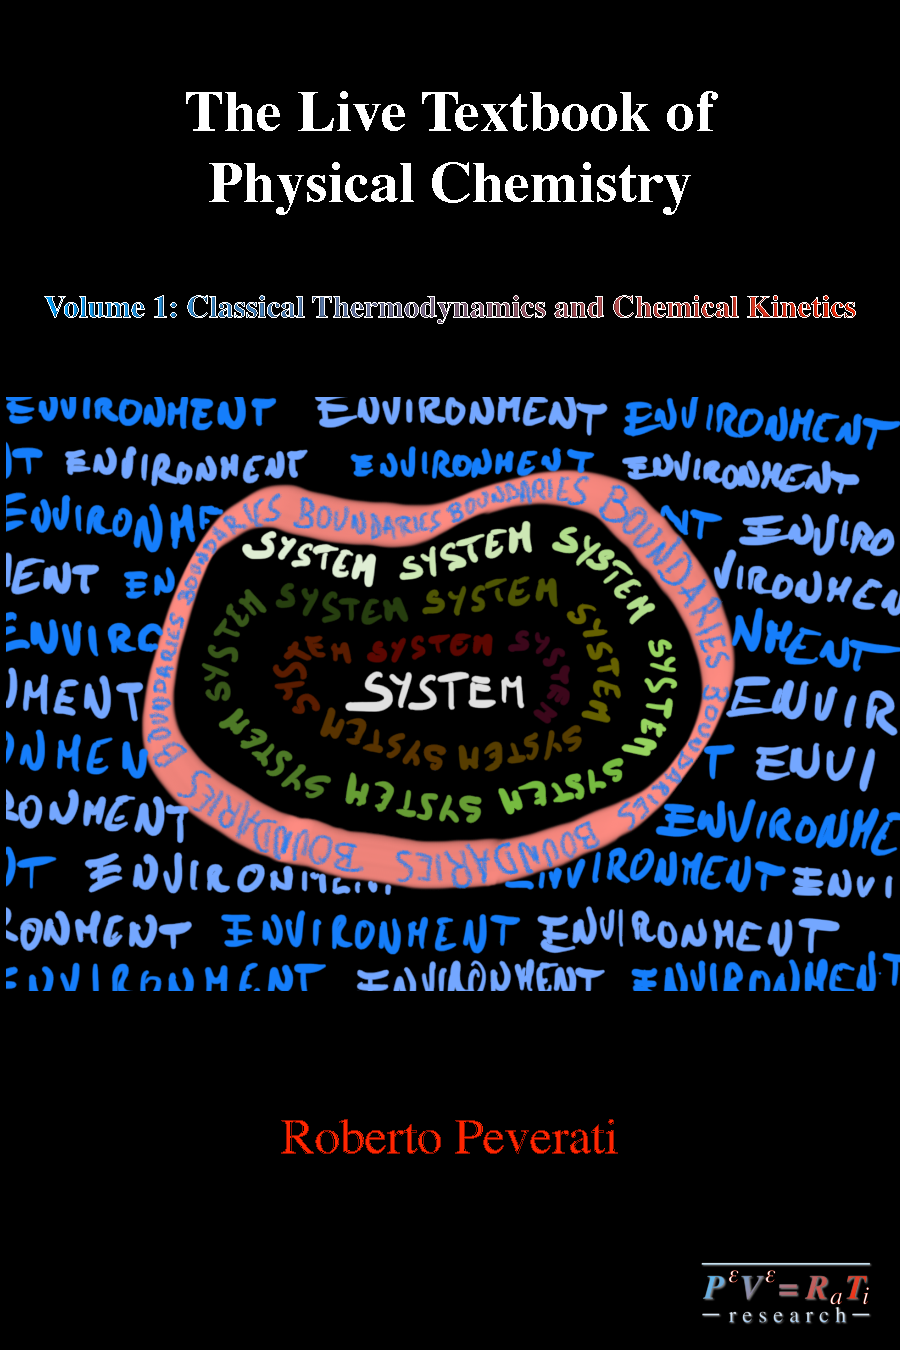
\includepdf[pages={1}, scale=1]{FrontPage_6x9.pdf}
%Frontpage for USLetter:
%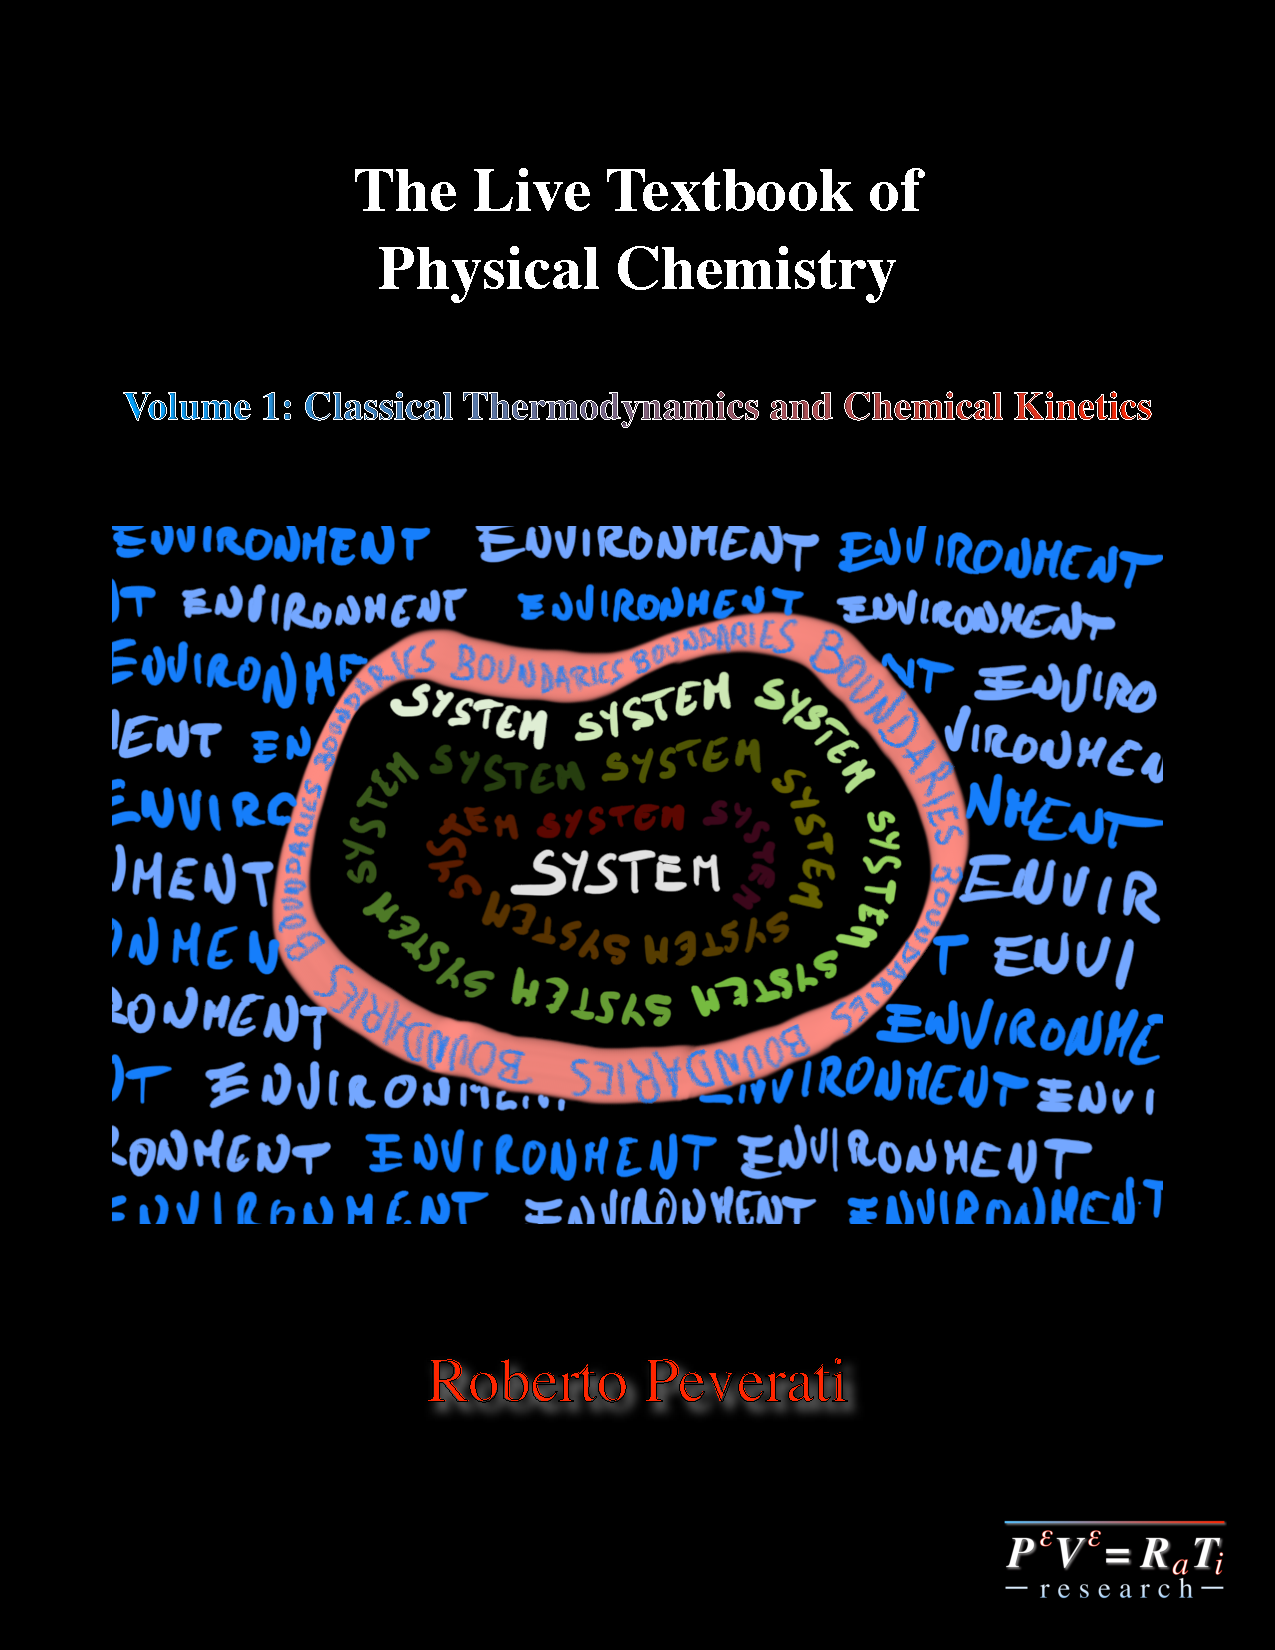
\includepdf[pages={1}, scale=1]{FrontPage.pdf}
\newpage

\let\maketitle\oldmaketitle

% Let's change \thepage so it prints one less than
% the real page number; \pagenumbering{arabic}
% will redefine it to the right meaning afterwards.
\renewcommand\thepage{\romannumeral\numexpr\value{page}-1\relax}


{
\setcounter{tocdepth}{1}
\tableofcontents
}
\renewcommand{\arraystretch}{1.8}

\hypertarget{preface}{%
\chapter*{Preface}\label{preface}}
\addcontentsline{toc}{chapter}{Preface}

\begin{center}
\includegraphics[width=0.8\linewidth]{./img/OEP_Figures.000} \end{center}

This textbook is the official textbook for the Physical Chemistry 1 Course (CHM 3001) at Florida Tech.

The instructor for this course and author of this textbook is Dr.~Roberto Peverati.

\textbf{Contacts}: \href{mailto:rpeverati@fit.edu}{\nolinkurl{rpeverati@fit.edu}}, Office: OPS 333, (321) 674-7735

Chemistry Program, Department of Biomedical and Chemical Engineering and Science
Florida Institute of Technology, Melbourne, FL.

\begin{quote}
This live open textbook is distributed under the \href{https://creativecommons.org/licenses/by-sa/4.0/}{CC-BY-SA 4.0 License} and it was funded by the Florida Tech Open Educational Resources Grant Program: A Collaboration of the Teaching Council, eEducation, and the Evans Library.
\end{quote}

\hypertarget{how-to-use-this-book}{%
\section*{How to use this book}\label{how-to-use-this-book}}
\addcontentsline{toc}{section}{How to use this book}

Please read this book carefully, since everything that will be in your exams is explained here.
Since this book is specifically tailored for the CHM 3001 course at Florida Tech, there are no superfluous parts. In other words, everything in it might be subject to question in the quizzes and the final exam.

\begin{quote}
Definitions and exercises are usually numbered and are highlighted in the text in this format (lighter grey, indented, and following a grey vertical bar). Please study the definitions carefully since they are fundamental concepts that will be used several times in the remainder of the text, and they will be subject to quizzes and exams. Exercises are essential for cementing the concepts, and you should attempt to execute them first without looking at the solution. Even if you were able to solve an exercise on your own, always read the solution after, since it might contain additional explanations expanding the main concepts in the text.
\end{quote}

Navigating the book should be straightforward. On each page, there is a useful sidebar on the left that gives you an overview of all chapters, and a toolbar at the top with important tools. Arrows to shift between chapters might also be present, depending on your browser. If you are old-school and prefer a pdf, you can download a printout by clicking on the toolbar's corresponding icon. If you are \emph{really} old-school and prefer a printed book, the best solution is to download the pdf and print it yourself. It is a LaTeX book, and I can promise you it will look good on paper. However, I cannot provide physical copies to each student. In the toolbar, you will find a useful search box that is capable of searching the entire book. The most adventurous will find in the toolbar a link to the raw GitHub source code. Feel free to head on \href{https://github.com/peverati/PChem1}{over there} and fork the book.

Each chapter of this book represents one week of work in the classroom and at home. The sidebar on the left will reflect your syllabus, as well as the main structure of the class on Canvas. The book is a live document, which means it will be updated throughout the semester with new material. While you are not required to check it every day, you might want to review each week's chapter before the lecture on Friday.

\begin{quote}
If you spot a mistake or a typo, contact Dr.~Peverati via \href{mailto:rpeverati@fit.edu}{email} and you will receive a credit of up to three points towards your final score, once the typo has been verified and corrected.
\end{quote}

\cleardoublepage
\pagenumbering{arabic}

\hypertarget{SystemVariables}{%
\chapter{Systems and Variables}\label{SystemVariables}}

\hypertarget{thermodynamic-systems}{%
\section{Thermodynamic Systems}\label{thermodynamic-systems}}

A thermodynamic system---or just simply a system---is a portion of space with defined boundaries that separate it from its surroundings (see also the title picture of this book). The surroundings may include other thermodynamic systems or physical systems that are not thermodynamic systems. A boundary may be a real physical barrier or a purely notional one. Typical examples of systems are reported in Figure \ref{fig:Fig1c1} below.\footnote{The photos depicted in this figure are taken from \href{https://en.wikipedia.org}{Wikipedia}: the Erlenmeyer flasks photo was taken by user Maytouch L., and distributed under CC-BY-SA license; the cloud photo was taken by user \href{https://commons.wikimedia.org/wiki/User:Matthew_T_Rader}{Mathew T Rader}, and distributed under CC-BY-SA license; the flame picture was taken by user \href{https://commons.wikimedia.org/wiki/User:Oscar}{Oscar}, and distributed under CC-BY-SA license; the balloon photo is in the public domain.}

\begin{figure}

{\centering 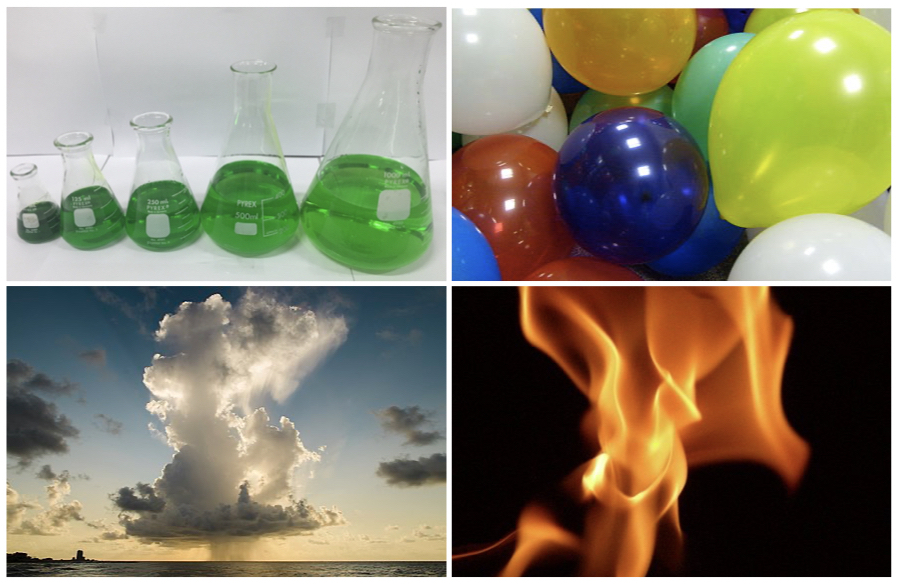
\includegraphics[width=0.7\linewidth]{./img/OEP_Figures.001} 

}

\caption{Examples of Thermodynamic Systems.}\label{fig:Fig1c1}
\end{figure}

In the first case, a liquid is contained in a typical Erlenmeyer flask. The boundaries of the system are the glass walls of the beaker. The second system is represented by the gas contained in a balloon. The boundary is a physical barrier also in this case, being the plastic of the balloon. The third case is that of a thunder cloud. The boundary is not a well-defined physical barrier, but rather some condition of pressure and chemical composition at the interface between the cloud and the atmosphere. Finally, the fourth case is the case of an open flame. In this case, the boundary is again non-physical, and possibly even harder to define than for a cloud. For example, we can choose to define the flame based on some temperature threshold, color criterion, or even some chemical one. Despite the lack of physical boundaries, the cloud and the flame---as portions of space containing matter---can be defined as a thermodynamic system.

A system can exchange exclusively mass, exclusively energy, or both mass and energy with its surroundings. Depending on the boundaries' ability to transfer these quantities, a system is defined as open, closed, or isolated. An open system exchanges both mass and energy. A closed system exchanges only energy, but not mass. Finally, an isolated system does not exchange mass nor energy.

When a system exchanges mass or energy with its surroundings, some of its parameters (variables) change. For example, if a system loses mass to the surroundings, the number of molecules (or moles) in the system will decrease. Similarly, if a system absorbs some energy, one or more of its variables (such as its temperature) increase. Mass and energy can flow into the system or out of the system. Let's consider mass exchange only. If some molecules of a substance leave the system, and then the same amount of molecules flow back into the system, the system will not be modified. We can count, for example, 100 molecules leaving a system and assign them the value of --100 in an outgoing process, and then observe the same 100 molecules going back into the system and assign them a value of +100. Regardless of the number of molecules present in the system in the first place, the overall balance will be --100 (from the outgoing process) +100 (from the ingoing process) = 0, which brings the system to its initial situation (mass has not changed). However, from a mathematical standpoint, we could have equally assigned the label +100 to the outgoing process and --100 to the ingoing one, and the overall total would have stayed the same: +100--100 = 0. Which of the two labels is best? For this case, it seems natural to define a mass going out of the system as negative (the system is losing it), and a mass going into the system as positive (the system is gaining it), but is it as straightforward for energy?

\begin{longtable}[]{@{}lcc@{}}
\toprule
\textbf{Type of System} & \textbf{Mass} & \textbf{Energy} (either heat or work)\tabularnewline
\midrule
\endhead
\textbf{Open} & Y & Y\tabularnewline
\textbf{Closed} & N & Y\tabularnewline
\textbf{Isolated} & N & N\tabularnewline
\bottomrule
\end{longtable}

\begin{quote}
Here is another example. Let's consider a system that is composed of your body. When you exercise, you lose mass in the form of water (sweat) and CO\textsubscript{2} (from respiration). This mass loss can be easily measured by stepping on a scale before and after exercise. The number you observe on the scale will go down. Hence you have lost weight. After exercise, you will reintegrate the lost mass by drinking and eating. If you have reinstated the same amount you have lost, your weight will be the same as before the exercise (no weight loss). Nevertheless, which label do you attach to the amounts that you have lost and gained? Let's say that you are running a 5 km race without drinking nor eating, and you measure your weight dropping 2 kg after the race. After the race, you drink 1.5 kg of water and eat a 500 g energy bar. Overall you did not lose any weight, and it would seem reasonable to label the 2 kg that you've lost as negative (--2) and the 1.5 kg of water that you drank and the 500 g bar that you ate as positive (+1.5 +0.5 = +2). But is it the only way? After all, you didn't gain nor lose any weight, so why not calling the 2 kg due to exercise +2 and the 2 that you've ingested as --2? It might seem silly, but mathematically it would not make any difference, the total would still be zero. Now, let's consider energy instead of mass. To run the 5km race, you have spent 500 kcal, which then you reintegrate precisely by eating the energy bar. Which sign would you put in front of the kilocalories that you ``burned'' during the race? In principle, you've lost them, so if you want to be consistent, you should use a negative sign. But if you think about it, you've put quite an effort to ``lose'' those kilocalories, so it might not feel bad to assign them a positive sign instead. After all, it's perfectly OK to say, ``I've done a 500 kcal run today'', while it might sound quite awkward to say, ``I've done a --500 kcal run today.'' Our previous exercise with mass demonstrates that it doesn't really matter which sign you put in front of the quantities. As long as you are consistent throughout the process, the signs will cancel out. If you've done a +500 kcal run, you've eaten a bar for --500 kcal, resulting in a total zero loss/gain. Alternatively, if you've done a --500 kcal run, you would have eaten a +500 kcal bar, for a total of again zero loss/gain.
\end{quote}

These simple examples demonstrate that the sign that we assign to quantities that flow through a boundary is arbitrary (i.e., we can define it any way we want, as long as we are always consistent with ourselves). There is no best way to assign those signs. If you ask two different people, you might obtain two different answers. But we are scientists, and we must make sure to be rigorous. For this reason, chemists have established a convention for the signs that we will follow throughout this course. If we are consistent in following the convention, we are guaranteed to never make any mistake with the signs.

\begin{quote}
\begin{definition}
\protect\hypertarget{def:chemistryconv}{}{\label{def:chemistryconv} }\emph{The chemistry convention of the sign is system-centric:}\footnote{Notice that physicists use a different sign convention when it comes to thermodynamics. To eliminate confusion, I will not describe the physics convention here, but if you are reading thermodynamics on a physics textbook, or if you are browsing the web and stumble on thermodynamics formula (e.g., on Wikipedia), please be advised that some quantity, such as work, might have a different sign than the one that is used in this textbook. Obviously, the science will not change, but you need to be \emph{always} consistent, so if you decide that you want to use the physics convention, make sure to \emph{always} use the physics convention. In this course, on the other hand, we will \emph{always} use the chemistry one, as introduced above.}

\begin{itemize}
\tightlist
\item
  \emph{If something (energy or mass) goes \textbf{into} the system it has a \textbf{positive} sign (the system is gaining)}
\item
  \emph{If something (energy or mass) goes \textbf{out of} the system it has a \textbf{negative} sign (the system is losing)}
\end{itemize}
\end{definition}
\end{quote}

If you want a trick to remember the convention, use the weight loss/gain during the exercise example above. You are the system, if you lose weight, the kilograms will be negative (--2 kg), while if you gain weight, they will be positive (+2 kg). Similarly, if you eat an energy bar, you are the system, and you will have increased your energy by +500 kcal (positive). In contrast, if you burned energy during exercise, you are the system, and you will have lost energy, hence --500 kcal (negative). If the system is a balloon filled with gas, and the balloon is losing mass, you are the balloon, and you are losing weight; hence the mass will be negative. If the balloon is absorbing heat (likely increasing its temperature and increasing its volume), you are the system, and you are gaining heat; hence heat will be positive.

\hypertarget{thermodynamic-variables}{%
\section{Thermodynamic Variables}\label{thermodynamic-variables}}

The system is defined and studied using parameters that are called variables. These variables are quantities that we can measure, such as pressure and temperature. However, don't be surprised if, on some occasions, you encounter some variable that is a little harder to measure directly, such as entropy. The variables depend only on the current state of the system, and therefore they define it. If I know the values of all the ``relevant variables'' of a system, I know the state of the system. The relationship between the variables is described by mathematical functions called state functions, while the ``relevant variables'' are called natural variables.

What are the ``relevant variables'' of a system? The answer to this question depends on the system, and it is not always straightforward. The simplest case is the case of an ideal gas, for which the natural variables are those that enter the ideal gas law and the corresponding equation:

\begin{equation}
  PV=nRT       
  \label{eq:idealgaslaworiginal}
\end{equation}

Therefore, the natural variables for an ideal gas are the pressure P, the volume V, the number of moles n, and the temperature T, with R being the ideal gas constant. Recalling from the general chemistry courses, R is a universal dimensional constant which has the values of R = 8.31 kJ/mol in SI units.\\
We will use the ideal gas equation and its variables as an example to discuss variables and functions in this chapter. We will analyze more complicated cases in the next chapters.
Variables can be classified according to numerous criteria, each with its advantages and disadvantages. A typical classification is:

\begin{itemize}
\tightlist
\item
  \textbf{Physical variables} (\(P\), \(V\), \(T\) in the ideal gas law): independent of the chemical composition of the system.
\item
  \textbf{Chemical variables} (\(n\) in the ideal gas law): dependent on the chemical composition of the system.
\end{itemize}

Another useful classification is:

\begin{itemize}
\tightlist
\item
  \textbf{Intensive variables} (\(P\), \(T\) in the ideal gas law): independent of the physical size (extension) of the system.
\item
  \textbf{Extensive variables} (\(V\), \(n\) in the ideal gas law): dependent on the physical size (extension) of the system.
\end{itemize}

When we deal with thermodynamic systems, it is more convenient to work with intensive variables. Luckily, it is relatively easy to convert extensive variables into intensive ones by just taking the ratio between the two of them. For an ideal gas, by taking the ratio between V and n, we obtained the intensive variable called molar volume:

\begin{equation}
  \overline{V}=\frac{V}{n}.   
  \label{eq:Vmdef}
\end{equation}

We can then recast eq. \eqref{eq:idealgaslaworiginal} as:

\begin{equation}
  P\overline{V}=RT,
  \label{eq:idealgaslaw}
\end{equation}

which is the preferred equation that we will use for the remainder of this course.
The ideal gas equation connects the 3 variables pressure, molar volume, and temperature, reducing the number of independent variables to just 2. In other words, once 2 of the 3 variables are known, the other one can be easily obtained using these simple relations:

\begin{equation}
  P(T,\overline{V})=\frac{RT}{\overline{V}},
  \label{eq:PTVm}
\end{equation}

\begin{equation}
  \overline{V}(T,P)=\frac{RT}{P},
  \label{eq:VmTP}
 \end{equation}

\begin{equation}
  T(P,\overline{V})=\frac{P\overline{V}}{R}.
  \label{eq:TPVm}
\end{equation}

These equations define three state functions, each one expressed in terms of two independent natural variables. For example, eq. \eqref{eq:PTVm} defines the state function called ``pressure'', expressed as a function of temperature and molar volume. Similarly, eq. \eqref{eq:VmTP} defines the ``molar volume'' as a function of temperature and pressure, and eq. \eqref{eq:TPVm} defines the ``temperature'' as a function of pressure and molar volume. When we know the natural variables that define a state function, we can express the function using its total differential, for example for the pressure \(P(T, \overline{V})\):

\begin{equation}
  dP=\left( \frac{\partial P}{\partial T} \right)dT + \left( \frac{\partial P}{\partial \overline{V}} \right)d\overline{V}
  \label{eq:totaldifferentialP}
\end{equation}

Recalling Schwartz's theorem, the mixed partial second derivatives that can be obtained from eq. 1.2.7 are the same:

\begin{equation}
  \frac{\partial^2 P}{\partial T \partial \overline{V}}=\frac{\partial}{\partial \overline{V}}\frac{\partial P}{\partial T}=\frac{\partial}{\partial T}\frac{\partial P}{\partial \overline{V}}=\frac{\partial^2 P}{\partial \overline{V} \partial T}
  \label{eq:schwartzP}
\end{equation}

Which can be easily verified considering that:

\begin{equation}
  \frac{\partial}{\partial \overline{V}} \frac{\partial P}{\partial T}  = \frac{\partial}{\partial \overline{V}} \left(\frac{R}{\overline{V}}\right) = -\frac{R}{\overline{V}^2} 
  \label{eq:secondderPA}
\end{equation}

and

\begin{equation}
  \frac{\partial}{\partial T} \frac{\partial P}{\partial \overline{V}}  = \frac{\partial}{\partial T} \left(\frac{-RT}{\overline{V}^2}\right) = -\frac{R}{\overline{V}^2} 
  \label{eq:secondderPB}
\end{equation}

While for the ideal gas law, all the variables are ``well-behaved'' and always satisfy Schwartz's theorem, we will encounter some variable for which Schwartz's theorem does not hold. Mathematically, if the Schwartz's theorem is violated (i.e., if the mixed second derivatives are not equal), then the corresponding function cannot be integrated, hence it is not a state function. The differential of a function that cannot be integrated cannot be defined exactly. Thus, these functions are called path functions; that is, they depend on the path rather than the state. The most typical examples of path functions that we will encounter in the next chapters are heat (\(Q\)) and work (\(W\)). For these functions, we cannot define exact differentials \(dQ\) and \(dW\), and we must introduce a new notation to define their ``inexact differentials'' \(đ Q\) and \(đ W\).

\begin{quote}
We will return to exact and inexact differential when we discuss heat and work, but for this chapter, it is crucial to notice the difference between a state function and a path function. A typical example to understand the difference between state and path function is to consider the distance between two geographical locations. Let's, for example, consider the distance between New York City and Los Angeles. If we fly straight from one city to the other, there are roughly 4,000 km between them. This ``air distance'' depends exclusively on the geographical location of the two cities. It stays constant regardless of the method of transportation that I have accessibility to travel between them. Since the cities' positions depend uniquely on their latitudes and longitudes, the ``air distance'' is a state function, i.e., it is uniquely defined from a simple relationship between measurable variables. However, the ``air distance'' is not the distance that I will practically have to drive when I go from NYC to LA. Such ``travel distance'' depends on the method of transportation that I decide to take (airplane vs.~car vs.~train vs.~boat vs.~\ldots). It will depend on a plentiful amount of other factors such as the choice of the road to be traveled (if going by car), the atmospheric conditions (if flying), and so on. A typical ``travel distance'' by car is, for example, about 4,500 km, which is about 12\% more than the ``air distance.'' Indeed, we could even design a very inefficient road trip that avoids all highways and will result in a ``travel distance'' of 8,000 km or even more (200\% of the ``air distance''). The ``travel distance'' is a clear example of a path function because it depends on the specific path that I decide to travel to go from NYC to LA. See Figure \ref{fig:Fig2c1}.
\end{quote}

\begin{figure}

{\centering 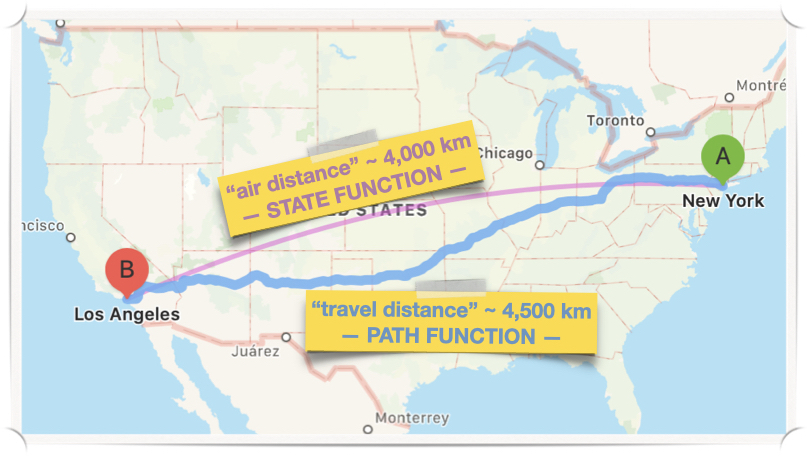
\includegraphics[width=0.6\linewidth]{./img/OEP_Figures.002} 

}

\caption{State Functions vs. Path Functions.}\label{fig:Fig2c1}
\end{figure}

\hypertarget{ZerothLaw}{%
\chapter{Zeroth Law of Thermodynamics}\label{ZerothLaw}}

\hypertarget{what-is-thermodynamics}{%
\section{What is Thermodynamics?}\label{what-is-thermodynamics}}

Thermodynamics is the branch of science that deals with heat and work, and their relation to energy. As the definition suggests, thermodynamics is concerned with two types of energy: heat and work. A formal definition of these forms of energy is as follow:

\begin{itemize}
\tightlist
\item
  Work is exchanged if external parameters are changed during the process.
\item
  Heat is exchanged if only internal parameters are changed during the process.
\end{itemize}

As we saw in chapter \ref{SystemVariables}, heat and work are not ``well-behaved'' quantities because they are path functions. On the one hand, it might be simple to measure the amount of heat and/or work experimentally, these measured quantities cannot be used to define the state of a system. Since heat and work are path functions, their values depend directly on the methods used to transfer them (their paths). Understanding and quantifying these energy transfers is the reason why thermodynamics was developed in the first place. The origin of thermodynamics dates back to the seventeenth century when people began to use heat and work for technological applications. These early scientists needed a mathematical tool to understand how heat and work were related to each other, and how they were related to the other variables that they were able to measure, such as temperature and volume.

Before we even discuss the definition of energy and how it relates to heat and work, it is crucial to introduce the essential concept of temperature. Temperature is an intuitive concept that has a surprisingly complex definition at the microscopic level.\footnote{In fact, we will not even give a rigorous microscopic definition of temperature within this textbook.} However, for all our purposes, it is not essential to have a microscopic definition of temperature, as long as we have the guarantee that this quantity can be measured unambiguously. In other words, we only need a mathematical definition of temperature that agrees with the physical existence of thermometers.

\hypertarget{the-zeroth-law-of-thermodynamics}{%
\section{The Zeroth Law of Thermodynamics}\label{the-zeroth-law-of-thermodynamics}}

The mathematical definition that guarantees that thermal equilibrium is an equivalence relation is called the zeroth law of thermodynamics. The zeroth law of thermodynamics states that if two thermodynamic systems are each in thermal equilibrium with a third one, then they are in thermal equilibrium with each other. The law might appear trivial and possibly redundant, but it is a fundamental requirement for the mathematical formulation of thermodynamics, so it needs to be stated. The zeroth law can be summarized by the following simple mathematical relation:

\begin{quote}
\begin{definition}
\protect\hypertarget{def:zerothlaw}{}{\label{def:zerothlaw} }\emph{Zeroth Law of Thermodynamics:} If \(T_A = T_B\), and \(T_B = T_C\), then \(T_A = T_C\).
\end{definition}
\end{quote}

Notice that when we state the zeroth law, it appears intuitive. However, this is not necessarily the case. Let's, for example, consider a pot of boiling water at \(P=1\;\mathrm{bar}\). Its temperature, \(T_{H_2O}\), is about 373 K. Let's now submerge in this water a coin made of wood and another coin made of metal. After some sufficient time, the wood coin will be in thermal equilibrium with the water, and its temperature \(T_W = T_{H_2O}\). Similarly, the metal coin will also be in thermal equilibrium with the water, hence \(T_M = T_{H_2O}\). According to the zeroth law, the temperature of the wood coin and that of the metal coin are precisely the same \(T_W = T_M = 373\;\mathrm{K}\), even if they are not in direct contact with each other. Now here's the catch: since wood and metal transmit heat in different manners if I take the coins out of the water and put them immediately in your hands, one of them will be very hot, but the other will burn you. If you had to guess the temperature of the two coins without a thermometer, and without knowing that they were immersed in boiling water, would you suppose that they have the same temperature? Probably not.

\hypertarget{workint}{%
\section{Calculation of Work}\label{workint}}

In thermodynamics, work (\(W\)) is the ability of a system to transfer energy by exerting a force on its surroundings. Work can be measured simply by evaluating its effects, such as displacing a massive object by some amount of space. The mathematical treatment of work, however, is complicated because \emph{work is a path function}. In the following sections, we will analyze how work is calculated in some prototypical situations commonly encountered in the thermodynamical treatment of systems.

\hypertarget{free-expansion-at-constant-temperature}{%
\subsection{Free expansion at constant temperature}\label{free-expansion-at-constant-temperature}}

\begin{figure}

{\centering 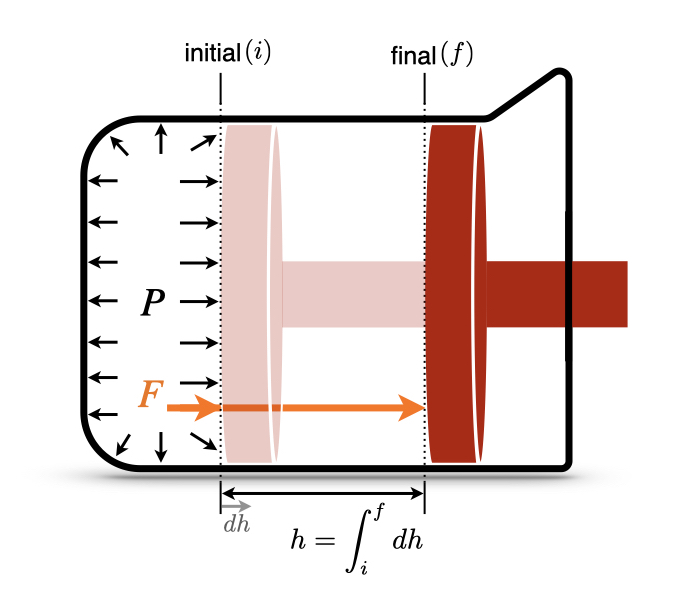
\includegraphics[width=0.5\linewidth]{./img/OEP_Figures.003} 

}

\caption{Free Expansion at Constant Temperature of an Ideal Gas.}\label{fig:Fig1c3}
\end{figure}

Let's consider the situation in Figure \ref{fig:Fig1c3}, where a special beaker with a piston that is free to move is filled with an ideal gas. The beaker sits in a horizontal position on a desk, so the piston is not subject to any external forces\footnote{For this simple thought experiment, we will ignore any external force that is not significant. In other words, we will not consider the friction of the piston on the beaker walls or any other foreign influence.}. The piston is initially compressed to a position that is not in equilibrium \((i)\). After the process, the piston reaches a final equilibrium position \((f)\). We assume that the only force acting on the piston is the pressure of the ideal gas, \(P\). How do we calculate the work (\(W\)) performed by the system?

From basic physics, we recall that the infinitesimal amount of work associated with an object moving in space is given by the force acting on the object (\(F\)) multiplied by the infinitesimal amount it gets displaced (\(d h\)):

\begin{equation}
  đ W = - Fdh,
  \label{eq:Wphysics}
\end{equation}

where the negative sign comes from the chemistry sign convention, Definition \ref{def:chemistryconv}, since the work in Figure \ref{fig:Fig1c3} is \emph{performed} by the system (expansion). What kind of force is moving the piston? It is the force due to the pressure of the gas. Relying upon another definition from physics, the pressure is the ratio between the force (\(F\)) and the area (\(A\)) that such force acts upon:

\begin{equation}
  P = F/A.
  \label{eq:Pphysics}
\end{equation}

Obtaining \(F\) from eq. \eqref{eq:Pphysics} and replacing it in eq. \eqref{eq:Wphysics}, we obtain:

\begin{equation}
  đ W = - P \underbrace{Adh}_{dV},
  \label{eq:Wphysics2}
\end{equation}

and considering that \(Adh\) (area times infinitesimal height) is the definition of an infinitesimal volume \(dV\), we obtain:

\begin{equation}
  đ W = - PdV,
  \label{eq:Wdef}
\end{equation}

If we want to calculate the amount of work performed by a system, \(W\), from eq. \eqref{eq:Wdef}, we need to recall that \(đ W\) is an inexact differential. As such, we cannot integrate it from initial to final as for the (exact) differential of a state function, because:

\begin{equation}
  \int_{i}^{f}đ W \neq W_f - W_i,
  \label{eq:Wdiff}
\end{equation}

but rather:

\begin{equation}
  \int_{\text{path}} đ W = W,
  \label{eq:Wdiff2}
\end{equation}

where the integration is performed along the \emph{path}. Using eq. \eqref{eq:Wdiff2}, we can integrate eq. \eqref{eq:Wdef} as:

\begin{equation}
  \int đ W = W = - \int_{i}^{f} PdV,
  \label{eq:Wint}
\end{equation}

where the integral on the left-hand side is taken along the path,\footnote{from here on we will replace the notation \(\int_{\text{path}}\) with the more convenient \(\int\) and we will keep in mind that the integral of an inexact differential must be taken along the path.} while the integral on the right-hand side can be taken between the initial and final states, since \(dV\) is a state function.
How do we solve the integral in eq. \eqref{eq:Wint}? The pressure in this process is not constant since it decreases throughout the process. Therefore \(P\) cannot be moved outside the integral. However, if our gas is ideal, we can calculate the pressure using the ideal gas law \(P=\frac{nRT}{V}\), and solve the integral because \(n\), \(R\), and \(T\) are constant:

\begin{equation}
  W = - nRT \int_{i}^{f} \frac{dV}{V} = -nRT \ln \frac{V_f}{V_i},
  \label{eq:WintsolvedV}
\end{equation}

which, considering that \(P_iV_i=P_fV_f\), can be also written as:

\begin{equation}
  W = -nRT \ln \frac{P_i}{P_f}.
  \label{eq:WintsolvedP}
\end{equation}

\hypertarget{isothermal-expansion-against-a-constant-external-pressure}{%
\subsection{Isothermal expansion against a constant external pressure}\label{isothermal-expansion-against-a-constant-external-pressure}}

\begin{figure}

{\centering 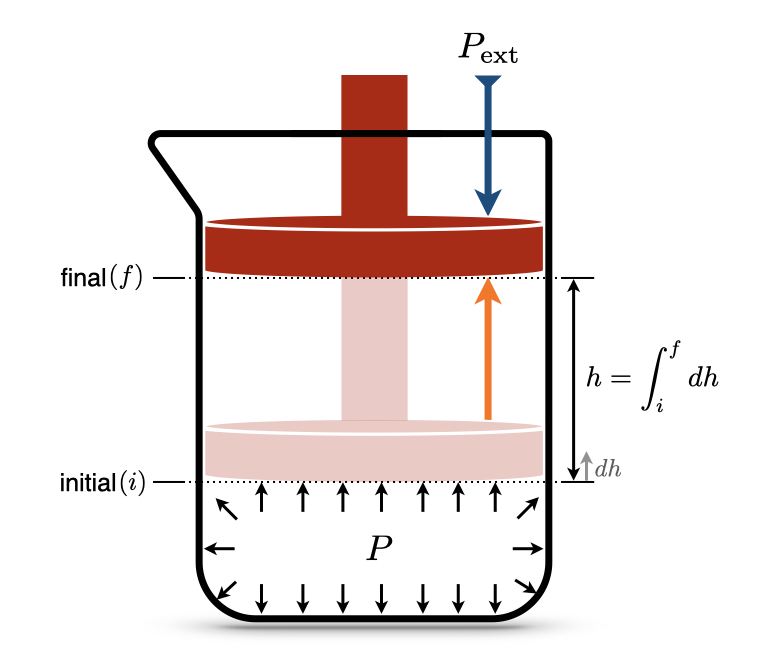
\includegraphics[width=0.5\linewidth]{./img/OEP_Figures.004} 

}

\caption{Isothermal Expansion of an Ideal Gas Against a Constant External Pressure.}\label{fig:Fig2c3}
\end{figure}

The process that we are analyzing here (Figure \ref{fig:Fig2c3}) is apparently similar to the case we have seen in the previous section, with the noticeable difference that the beaker now sits vertically on the workbench. In this case, when the piston moves upwards, it is no longer moving freely, but it moves against the force due to the constant external pressure \(P_{\text{ext}}\).

The integral that describes the work performed by the system in this case involves a transformation at constant external pressure:

\begin{equation}
  \int đ W = W = - \int_{i}^{f} P_{\text{ext}}dV,
  \label{eq:Wint2}
\end{equation}

which can be easily simplified as:

\begin{equation}
  W = - \int_{i}^{f} P_{\text{ext}}dV = -P_{\text{ext}} \int_{i}^{f} dV = -P_{\text{ext}} (V_f-V_i),
  \label{eq:Wint3}
\end{equation}

resulting in the following simple formula to calculate \(W\):

\begin{equation}
  W = -P_{\text{ext}} \Delta V,
  \label{eq:WintF}
\end{equation}

Comparing eq. \eqref{eq:WintF} with eq. \eqref{eq:WintsolvedP} shows how different this case is from the previous one.

\hypertarget{heatint}{%
\section{Calculation of Heat}\label{heatint}}

Heat (\(Q\)) is a property that gets transferred between substances. Similarly to work, the amount of heat that flows through a boundary can be measured, but its mathematical treatment is complicated because \emph{heat is a path function}.
As you probably recall from general chemistry, the ability of a substance to absorb heat is given by a coefficient called the heat capacity, which is measured in SI in \(\frac{\text{J}}{\text{mol K}}\). However, since heat is a path function, these coefficients are not unique, and we have different ones depending on how the heat transfer happens.

\hypertarget{processes-at-constant-volume-isochoric}{%
\subsection{Processes at constant volume (isochoric)}\label{processes-at-constant-volume-isochoric}}

The heat capacity at constant volume measures the ability of a substance to absorb heat at constant volume. Recasting from general chemistry:

\begin{quote}
The molar heat capacity at constant volume is the amount of heat required to increase the temperature of 1 mol of a substance by 1 K at constant volume.
\end{quote}

This simple definition can be written in mathematical terms as:

\begin{equation}
  C_V = \frac{đ Q_V}{n dT} \Rightarrow đ Q_V = n C_V dT.
  \label{eq:Cvdef}
\end{equation}

Given a known value of \(C_V\), the amount of heat that gets transfered can be easily calculated by measuring the changes in temperature, after integration of eq. \eqref{eq:Cvdef}:

\begin{equation}
  đ Q_V = n C_V dT \rightarrow \int đ Q_V = n \int_{T_i}^{T_F}C_V dT \rightarrow Q_V = n C_V \int_{T_i}^{T_F}dT,
  \label{eq:Cvint1}
\end{equation}

which, assuming \(C_V\) independent of temperature, simply becomes:

\begin{equation}
  Q_V \cong n C_V \Delta T.
  \label{eq:Cvint}
\end{equation}

\hypertarget{heatconstp}{%
\subsection{Processes at constant pressure (isobaric)}\label{heatconstp}}

Similarly to the previous case, the heat capacity at constant pressure measures the ability of a substance to absorb heat at constant pressure. Recasting again from general chemistry:

\begin{quote}
The molar heat capacity at constant pressure is the amount of heat required to increase the temperature of 1 mol of a substance by 1 K at constant pressure.
\end{quote}

And once again, this mathematical treatment follows:

\begin{equation}
  C_P = \frac{đ Q_P}{n dT} \Rightarrow đ Q_P = n C_P dT \rightarrow \int đ Q_P = n \int_{T_i}^{T_F}C_P dT,
  \label{eq:Cpdef}
\end{equation}

which result in the simple formula:

\begin{equation}
  Q_P \cong n C_P \Delta T.
  \label{eq:Cpint}
\end{equation}

\hypertarget{FirstLaw}{%
\chapter{First Law of Thermodynamics}\label{FirstLaw}}

\hypertarget{energyint}{%
\section{Calculation of Internal Energy Changes}\label{energyint}}

The internal energy (\(U\)) of a system is a thermodynamic state function defined as:

\begin{quote}
\begin{definition}
\protect\hypertarget{def:energy}{}{\label{def:energy} }\emph{Internal Energy:} Property of a system that can be either transferred or converted.
\end{definition}
\end{quote}

In the absence of chemical transformations, heat and work are the only two forms of energy that thermodynamics is concerned with. Keeping in mind Definition \ref{def:chemistryconv}, which gives the convention for the signs of heat and work, the internal energy of a system can be written as:

\begin{equation}
  U = Q + W,
  \label{eq:U}
\end{equation}

which we can write in differential form by considering that the internal energy is a state function, as:
\begin{equation}
  dU = đ Q + đ W,
  \label{eq:dU}
\end{equation}

which, using eq. \eqref{eq:Wdef} becomes:

\begin{equation}
  dU = đ Q - PdV.
  \label{eq:dUpdv}
\end{equation}

\hypertarget{isothermalE}{%
\subsection{Internal energy in isothermal processes}\label{isothermalE}}

To study the behavior of the internal energy in a process at constant temperature (\(dT=0\)), James Prescott Joule (1818--1889) created the apparatus depicted in Figure \ref{fig:FigJexp}.

\begin{figure}

{\centering 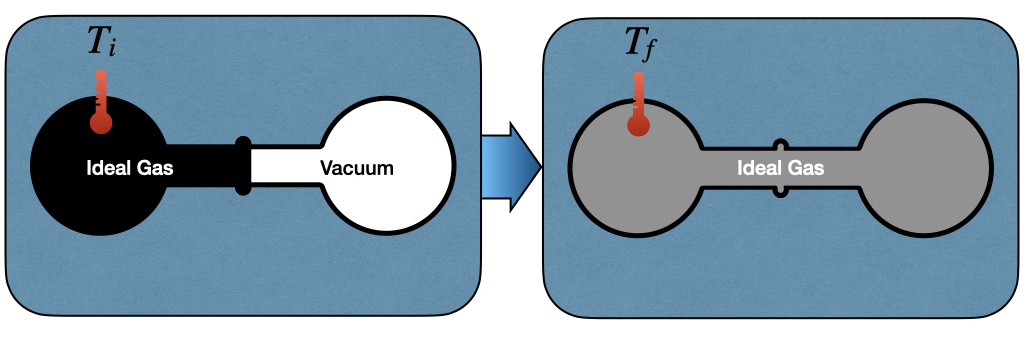
\includegraphics[width=0.8\linewidth]{./img/OEP_Figures.006} 

}

\caption{The Joule Expansion Experiment.}\label{fig:FigJexp}
\end{figure}

The left side of the Joule apparatus's inner chamber is filled with an ideal gas, while a vacuum is created in the right chamber. Both chambers are immersed in a water bath, to guarantee isolation from the environment. When the communication channel between the chambers is open, the gas expands and equilibrates. The work associated with the transformation is:

\begin{equation}
  đ W=P_{\text{ext}}dV = 0,
  \label{eq:JexpW}
\end{equation}

since the chambers are not in communication with the environment, \(P_{\text{ext}}=0\). Thus, changes in internal energy are associated with the heat transfer of the process, which can be measured by monitoring the temperature of the gas at the beginning, \(T_i\), and at the end of the experiment \(T_f\). Joule noticed experimentally that if he used an ideal gas for this experiment, the temperature would not change \(T_i = T_f\). Since the temperature doesn't change, there is no heat transfer, and therefore the internal energy stays constant:

\begin{equation}
  dU = đ Q = 0.
  \label{eq:JexpQU}
\end{equation}

\begin{quote}
Notice that Joule's conclusion is valid only for an ideal gas. If we expand a real gas, we do notice a change in temperature associated with the expansion. A typical example of this behavior is when you use a pressurized spray bottle and release its content for an extended time in the air. The container will typically get colder. We will discuss this behavior in chapter \ref{RealGases} when we will study non-ideal gases.
\end{quote}

From this simple experiment, we can conclude that the internal energy of an ideal gas depends only on its temperature.

\hypertarget{internal-energy-in-adiabatic-processes}{%
\subsection{Internal energy in adiabatic processes}\label{internal-energy-in-adiabatic-processes}}

An adiabatic process is defined as a process that happens without the exchange of heat. As such, \(đ Q=0\), and the work associated with an adiabatic process becomes a state function:

\begin{equation}
  dU=đ W=PdV,
  \label{eq:dUadiabatic}
\end{equation}

which can then be calculated using the formulas that we derived in section \ref{workint}. Notice that isothermal and adiabatic are two very different processes. While an adiabatic process happens without the exchange of heat across the system's boundaries, this does not mean that the system's temperature does not change. Isothermal processes are usually associated with a heat transfer across the boundaries to maintain the temperature of the system constant. For adiabatic processes, it is quite the opposite since they are usually associated with a change in temperature.

\hypertarget{internal-energy-in-isochoric-processes}{%
\subsection{Internal energy in isochoric processes}\label{internal-energy-in-isochoric-processes}}

An isocoric process is a process in which the volume does not change. Therefore, \(đ W=0\), and \(dU = đ Q_V\), which for 1 mol of substance and using eq. \eqref{eq:Cvdef}, becomes:

\begin{equation}
  dU = đ Q_V = n C_V dT.
  \label{eq:dUqv}
\end{equation}

Since no work is performed at these conditions, the heat becomes a state function. Eq. \eqref{eq:dUqv} also gives a mathematical justification of the concept of heat capacity at constant volume. \(C_V\) can now be interpreted as the partial derivative (a coefficient) of a state function (the internal energy):

\begin{equation}
  C_V = \left( \frac{\partial U} {\partial T} \right)_{V,n},
  \label{eq:cvstatefunc}
\end{equation}

where we have replaced the total derivative \(d\) with a partial one \(\partial\), and we have specified that the derivation happens at constant volume and number of moles. Eq. \eqref{eq:cvstatefunc} equation brings a rigorous definition of heat capacity at constant volume for 1 mol of substance:

\begin{quote}
\begin{definition}
\protect\hypertarget{def:newdefcv}{}{\label{def:newdefcv} }\emph{The heat capacity of a substance, \(C_V\), represents its ability to absorb \textbf{energy} at constant \textbf{volume}.}
\end{definition}
\end{quote}

\hypertarget{enthalpy}{%
\subsection{Internal energy in isobaric processes}\label{enthalpy}}

In an isobaric process, the pressure does not change, hence \(dP=0\). Unfortunately, eq. \eqref{eq:dU} for this case does not simplify further, as happened in the two previous cases. However, in section \ref{heatconstp}, we have introduced the useful concept of heat capacity at constant \(P\). \(C_P\) was used in an adiabatic process in the same manner as \(C_V\) was used in the isochoric case. That is, as a coefficient to measure the amount of heat absorbed at constant pressure. Eq. \eqref{eq:cvstatefunc} gave a mathematical definition of \(C_V\) as the partial derivative of a state function (the internal energy). But if heat capacities are coefficients, and coefficients are partial derivatives of state functions, how do we explain \(C_P\)? In order to do so, we can introduce a new state function, called the enthalpy (\(H\)), as:

\begin{equation}
  H = U + PV,
  \label{eq:enthalpydef}
\end{equation}

and its differential, calculated as:

\begin{equation}
  dH = dU + d(PV) = dU + PdV + \overbrace{VdP}^{0},
  \label{eq:enthalpydefdiff}
\end{equation}

which can be rearranged as:

\begin{equation}
  dU = dH -PdV,
  \label{eq:enthalpydefdiffu}
\end{equation}

Replacing eq. \eqref{eq:enthalpydefdiffu} into eq. \eqref{eq:dUpdv}:

\begin{equation}
  dH -PdV = đ Q_P - PdV,
  \label{eq:dh1}
\end{equation}

which simplifies to:

\begin{equation}
  dH = đ Q_P.
  \label{eq:dh2}
\end{equation}

Eq. \eqref{eq:dh2} establishes that the heat exchanged at constant pressure is equal to a new state function called the enthalpy, defined by eq. \eqref{eq:enthalpydef}. It also establishes a mathematical justification of the concept of heat capacity at constant pressure. Similarly to \(C_V\), \(C_P\) can now be interpreted as the partial derivative (a coefficient) of the new state function (the enthalpy):

\begin{equation}
  C_P = \left( \frac{\partial H} {\partial T} \right)_{P,n},
  \label{eq:cpstatefunc}
\end{equation}

Eq. \eqref{eq:cpstatefunc} brings also a rigorous definition of heat capacity at constant pressure for 1 mol of substance:

\begin{quote}
\begin{definition}
\protect\hypertarget{def:newdefcp}{}{\label{def:newdefcp} }\emph{The heat capacity of a substance, \(C_P\), represents its ability to absorb \textbf{enthalpy} at constant \textbf{pressure}.}
\end{definition}
\end{quote}

\hypertarget{the-first-law-of-thermodynamics}{%
\section{The First Law of Thermodynamics}\label{the-first-law-of-thermodynamics}}

We finally come to a working definition of the first law. If we take an isolated system---i.e., a system that does not exchange heat nor mass with its surroundings---its internal energy is conserved. If the internal energy is conserved, \(dU=0\). Therefore, for an isolated system:

\begin{equation}
  đ Q = -đ W,
  \label{eq:heateqwork}
\end{equation}

and heat and work can be easily calculated using any of the appropriate formulas introduced in either section \ref{workint} or \ref{heatint}.

The first law is a conservation law. It is intuitive since it comes directly from Lavoisier's principle of ``nothing is lost, nothing is created, everything is transformed.'' Considering that the only system that is truly isolated is the universe, we can condense the first law in one simple sentence:

\begin{quote}
\begin{definition}
\protect\hypertarget{def:firstlaw}{}{\label{def:firstlaw} }\emph{First Law of Thermodynamics:} The energy of the universe is conserved.
\end{definition}
\end{quote}

\hypertarget{reversible-and-irreversible-processes}{%
\section{Reversible and Irreversible processes}\label{reversible-and-irreversible-processes}}

\hypertarget{calculation-of-w_textmax-and-w_textmin}{%
\subsection{\texorpdfstring{Calculation of \(| W_{\text{max}} |\) and \(| W_{\text{min}} |\)}{Calculation of \textbar{} W\_\{\textbackslash text\{max\}\} \textbar{} and \textbar{} W\_\{\textbackslash text\{min\}\} \textbar{}}}\label{calculation-of-w_textmax-and-w_textmin}}

Let's go back to the calculation of the work in a process at constant temperature. We can use the formulas obtained in section \ref{workint} to understand a little bit better the meaning of a \emph{path function}. Let's consider the following PV diagram, obtained from an ideal gas at constant \(T=298\) K:

\begin{center}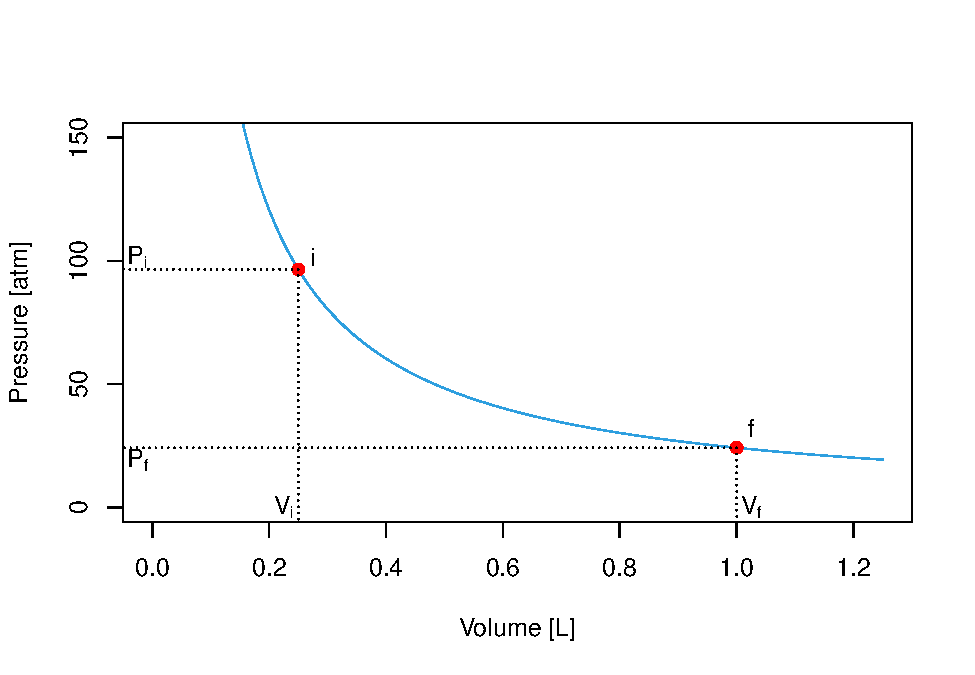
\includegraphics[width=0.7\linewidth]{pchem1_files/figure-latex/unnamed-chunk-2-1} \end{center}

where the isothermal expansion happens between \(P_i\) and \(P_f\). If the expansion happens in a one-step fast process, for example against a constant pressure \(P_f=P_{\text{ext}}\), the work is given by eq. \eqref{eq:WintF}. On the plot, the absolute value of the work\footnote{we use the absolute value to avoid confusions due to the fact that the expansion work is negative according to Definition \ref{def:chemistryconv}.} is represented by the red area:

\begin{center}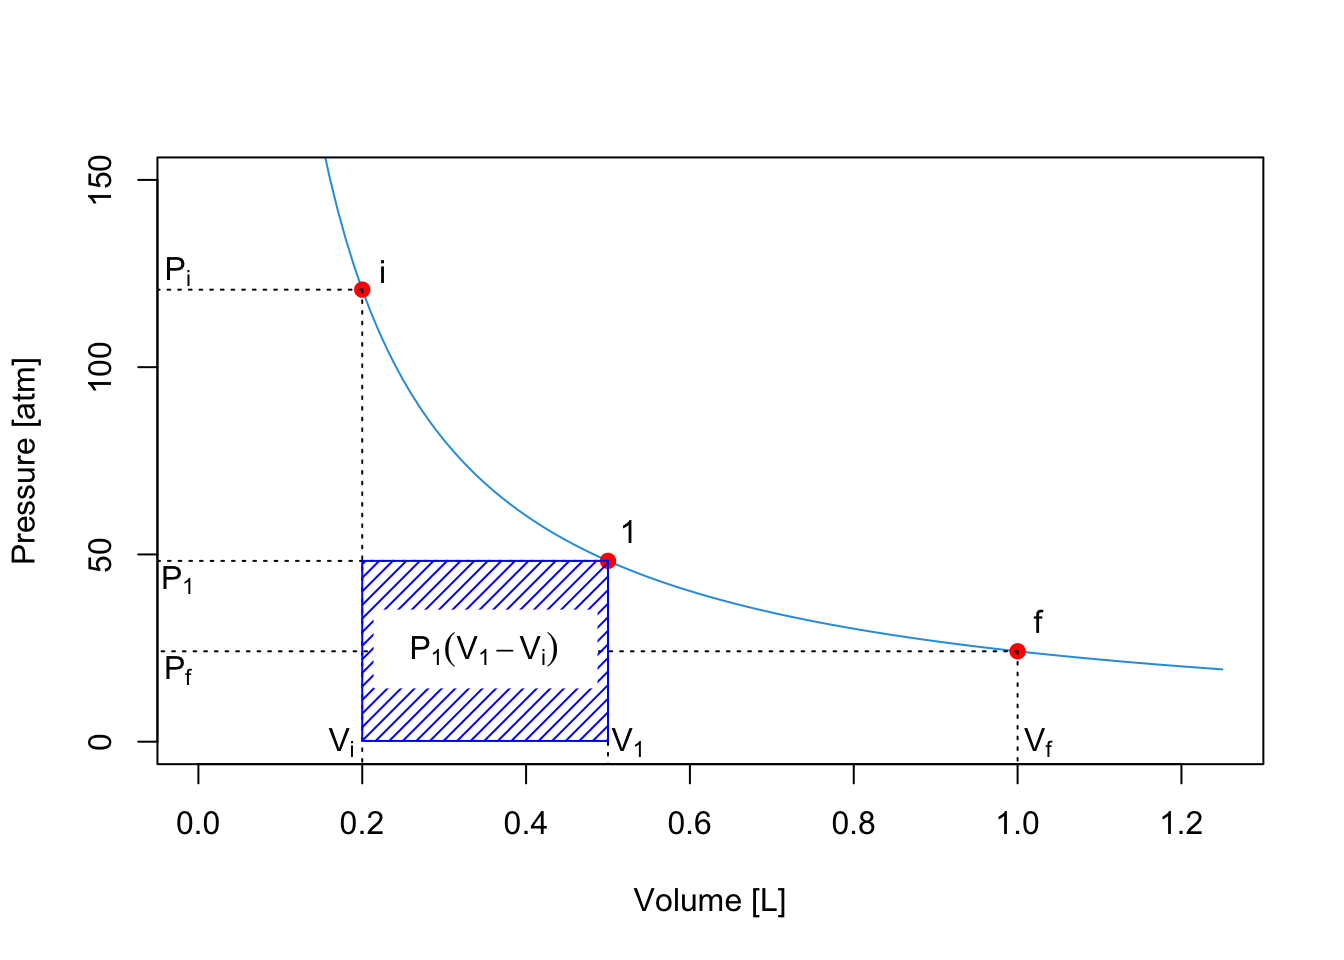
\includegraphics[width=0.7\linewidth]{pchem1_files/figure-latex/unnamed-chunk-3-1} \end{center}

\begin{equation}
\left| W_{\text{1-step}} \right| = P_{\text{ext}} (V_f-V_i)
  \label{eq:Warea1}
\end{equation}

However, if the process happens in two steps, by pausing at position (1) until equilibrium is reached, then we should calculate the work by dividing the process into two. The first process is an expansion between \(P\) and \(P_1\), whose absolute value of the work, \(W_A\), is represented by the blue area:

\begin{center}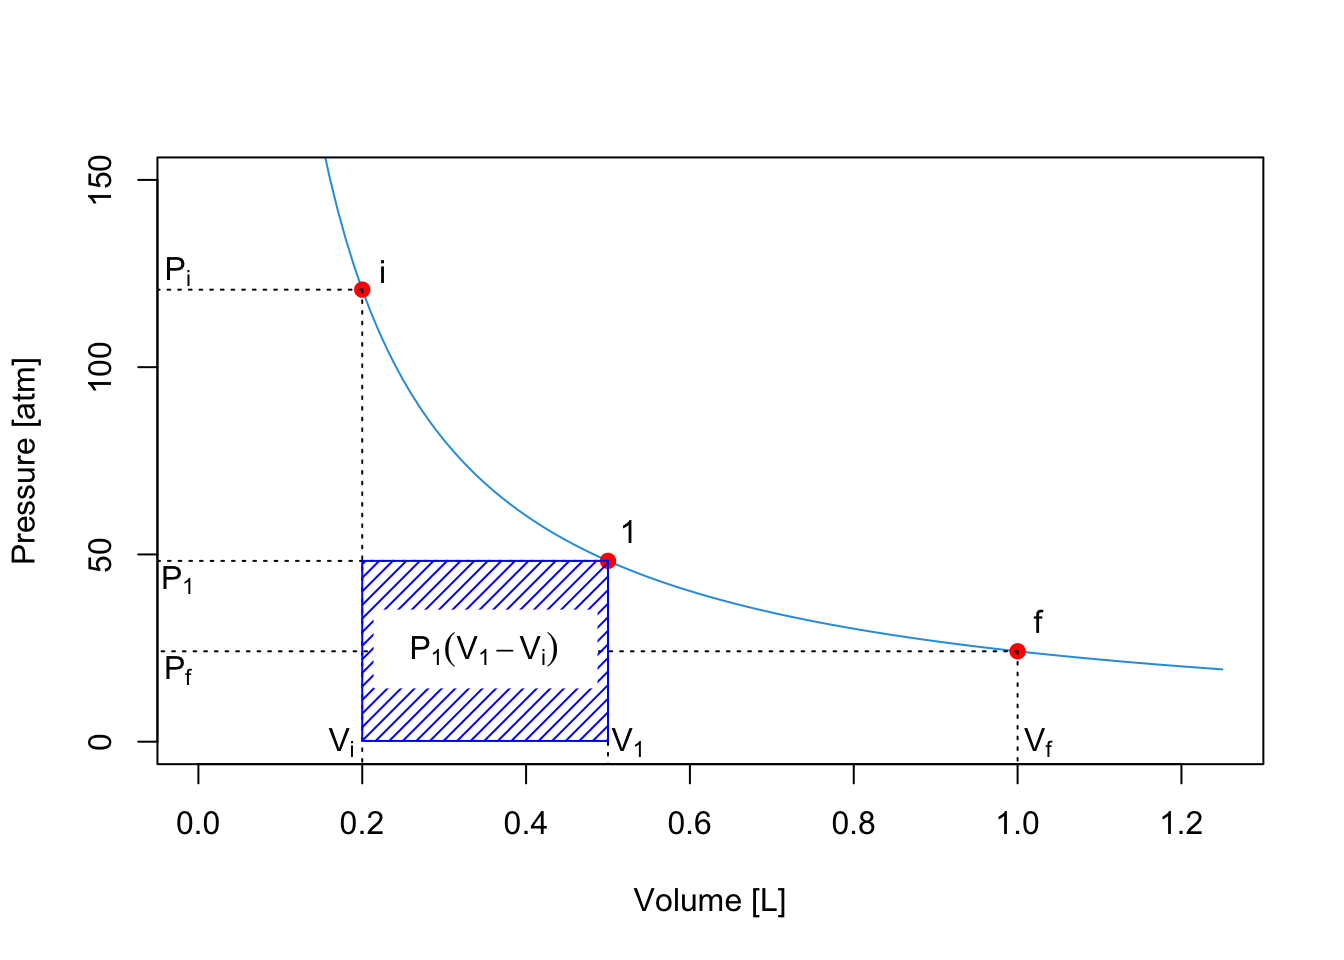
\includegraphics[width=0.7\linewidth]{pchem1_files/figure-latex/unnamed-chunk-4-1} \end{center}

\begin{equation}
\left| W_A \right| = P_1 (V_1-V_i)
  \label{eq:Warea2}
\end{equation}

The second process is an expansion between \(P_1\) and \(P_{\text{ext}}\), whose absolute value of the work is represented by the green area:

\begin{center}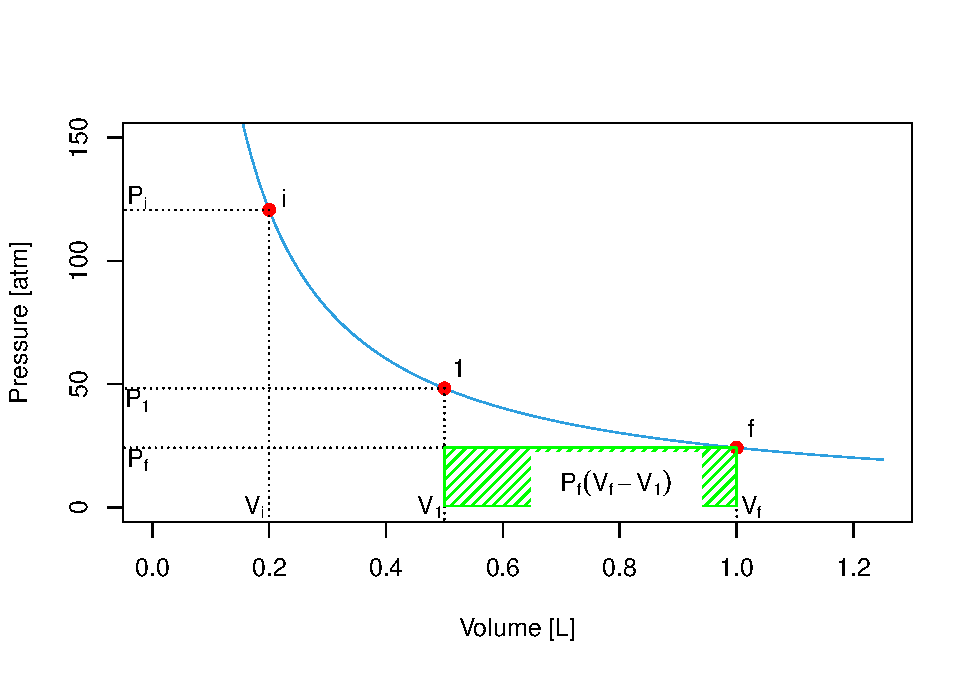
\includegraphics[width=0.7\linewidth]{pchem1_files/figure-latex/unnamed-chunk-5-1} \end{center}

\begin{equation}
\left| W_B \right| = P_f (V_f-V_1)
  \label{eq:Warea3}
\end{equation}

The total absolute value of the work for the 2-step process is given by the sum of the two areas:

\begin{center}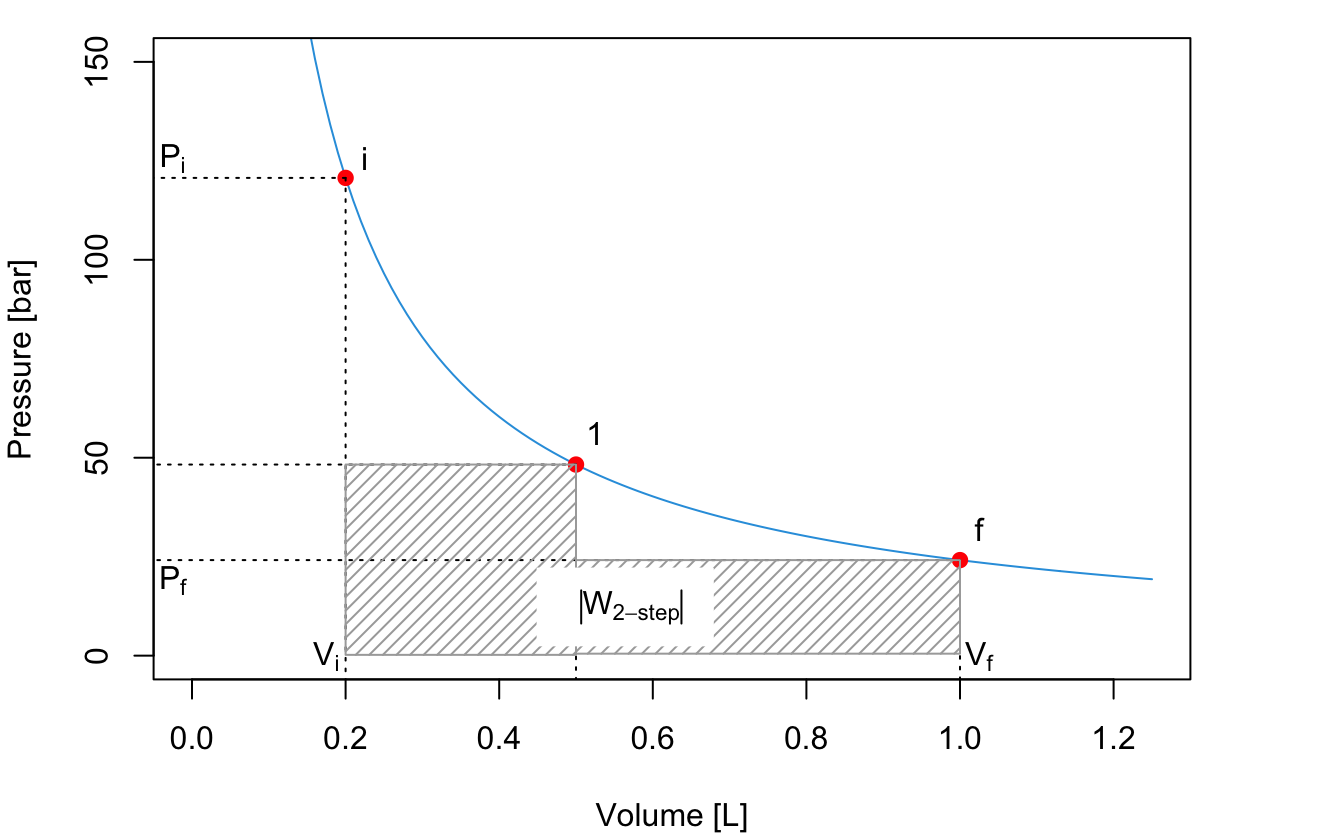
\includegraphics[width=0.7\linewidth]{pchem1_files/figure-latex/unnamed-chunk-6-1} \end{center}

\begin{equation}
  \left| W_{\text{2-step}} \right| = \left| W_A \right| + \left| W_B \right| = P_1 (V_1-V_i)+P_f (V_f-V_1).
  \label{eq:Warea4}
\end{equation}

As can be easily verified by comparing the shaded areas in the plots, \(\left| W_{\text{2-step}} \right| > \left| W_{\text{1-step}} \right|\).

We can easily extend this procedure to consider processes that happens in 3, 4, 5, \ldots, \(n\) steps. What is the limit of this procedure? In other words, what happens when \(n \rightarrow \infty\)? A simple answer is given by the plots in the next Figure, which clearly demonstrates that the maximum value of the area underneath the curve \(\left| W_{\text{max}}\right|\) is achieved in an \(\infty\)-step process, for which the work is calculated as:

\begin{equation}
  \left| W_{\infty \text{-step}} \right| = \left| W_{\text{max}} \right| = \sum_{n}^{\infty} P_n(V_n-V_{n-1}) = \int_{i}^{f} PdV.
  \label{eq:WintsolvedV2}
\end{equation}

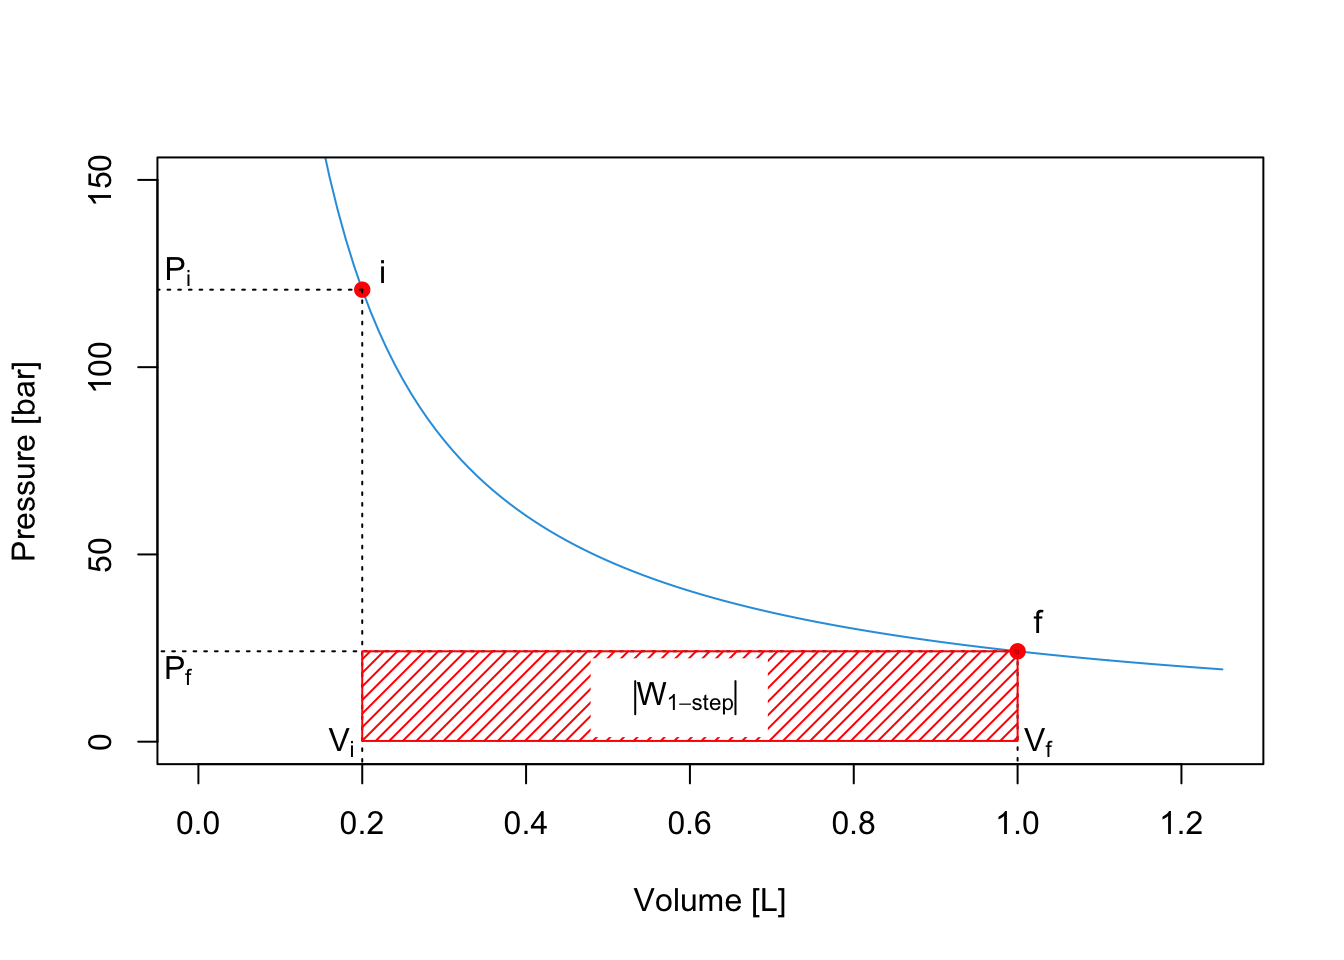
\includegraphics[width=0.5\linewidth,height=1\textheight]{pchem1_files/figure-latex/figures-side-1} 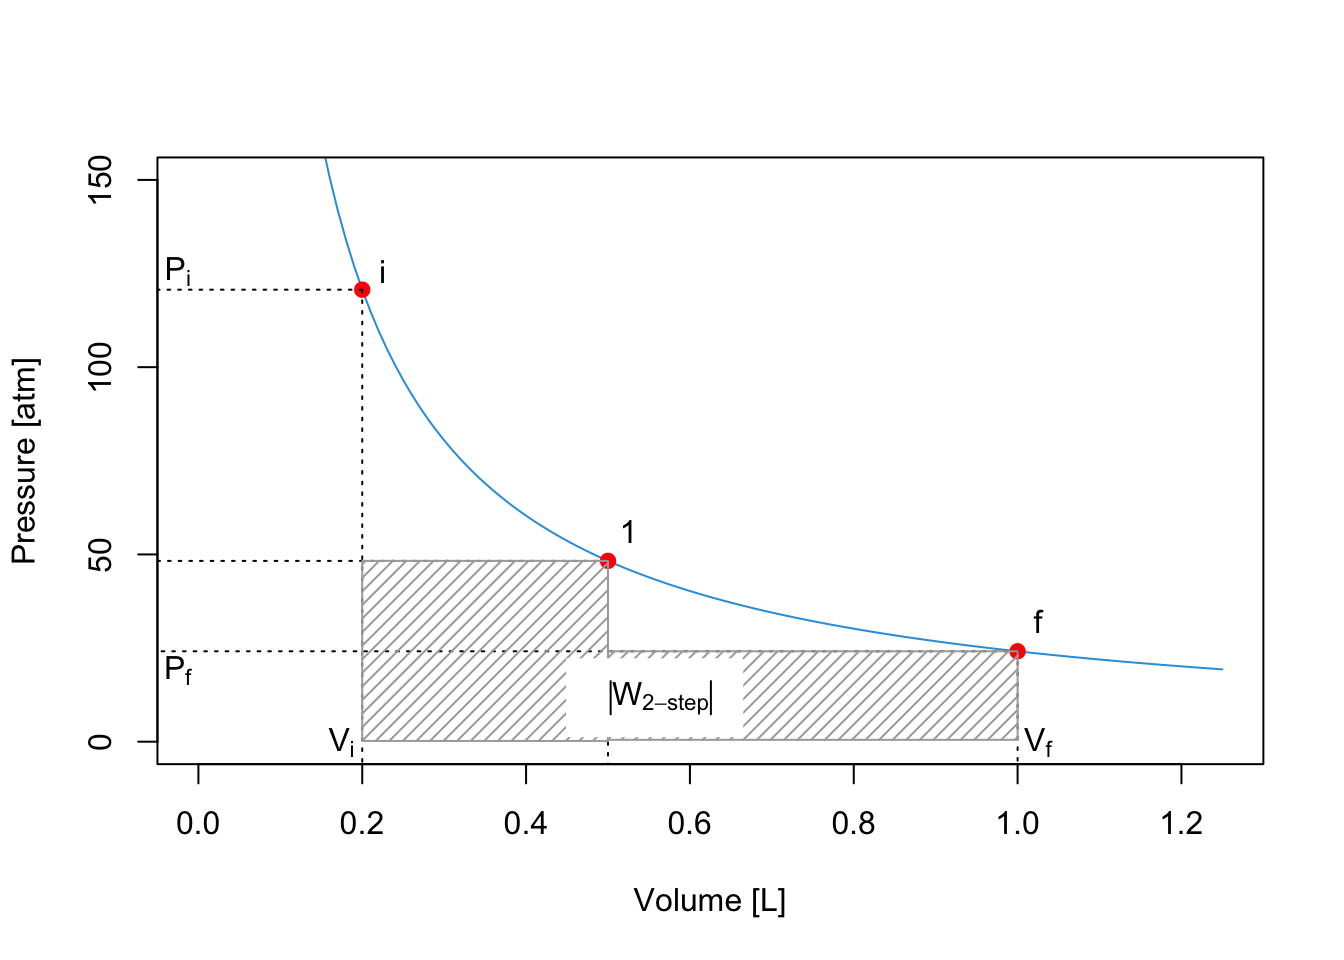
\includegraphics[width=0.5\linewidth,height=1\textheight]{pchem1_files/figure-latex/figures-side-2} 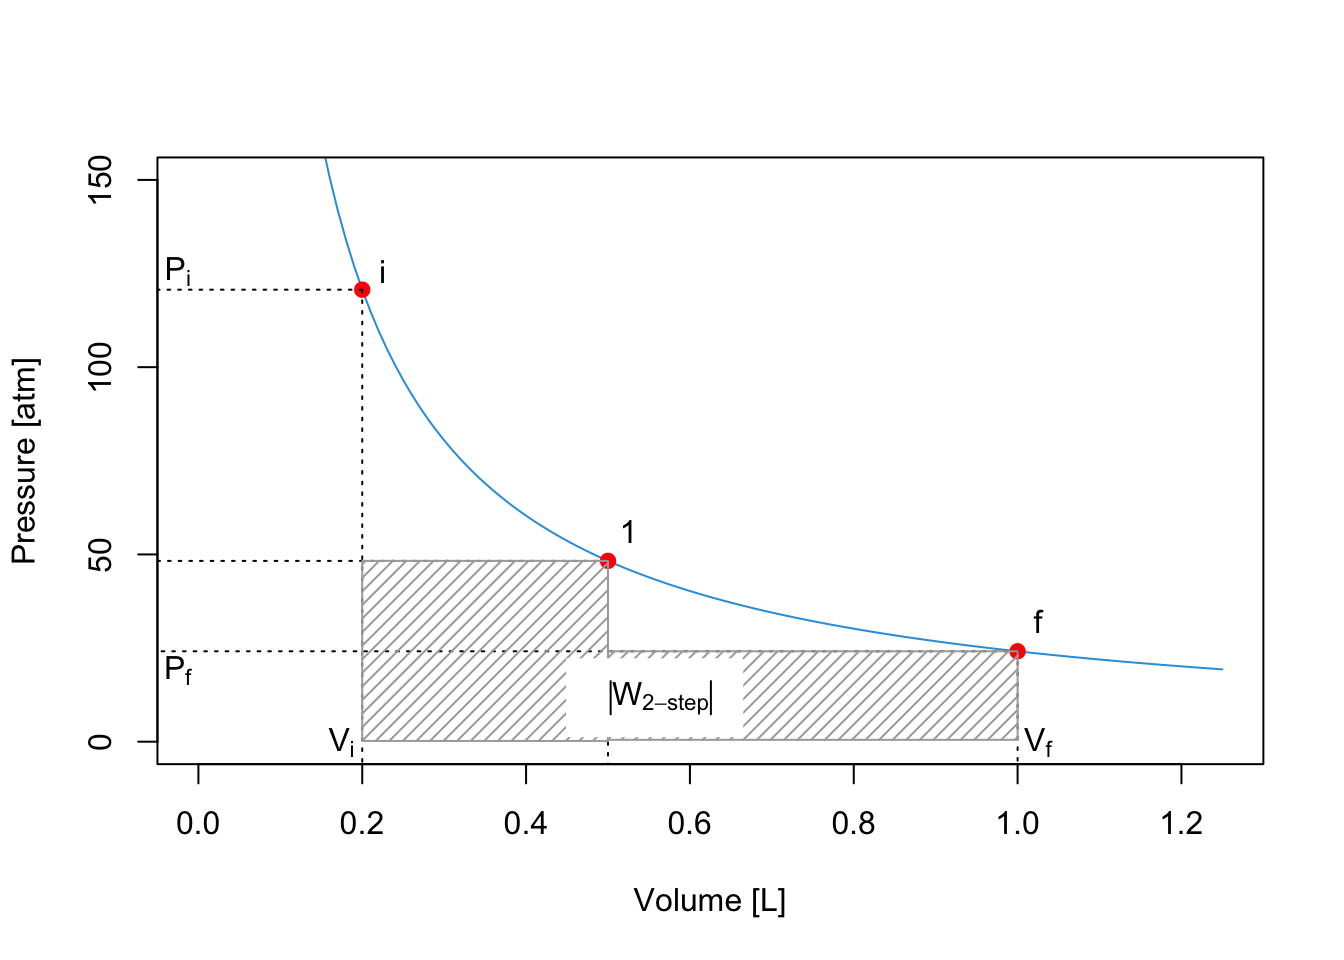
\includegraphics[width=0.5\linewidth,height=1\textheight]{pchem1_files/figure-latex/figures-side-3} 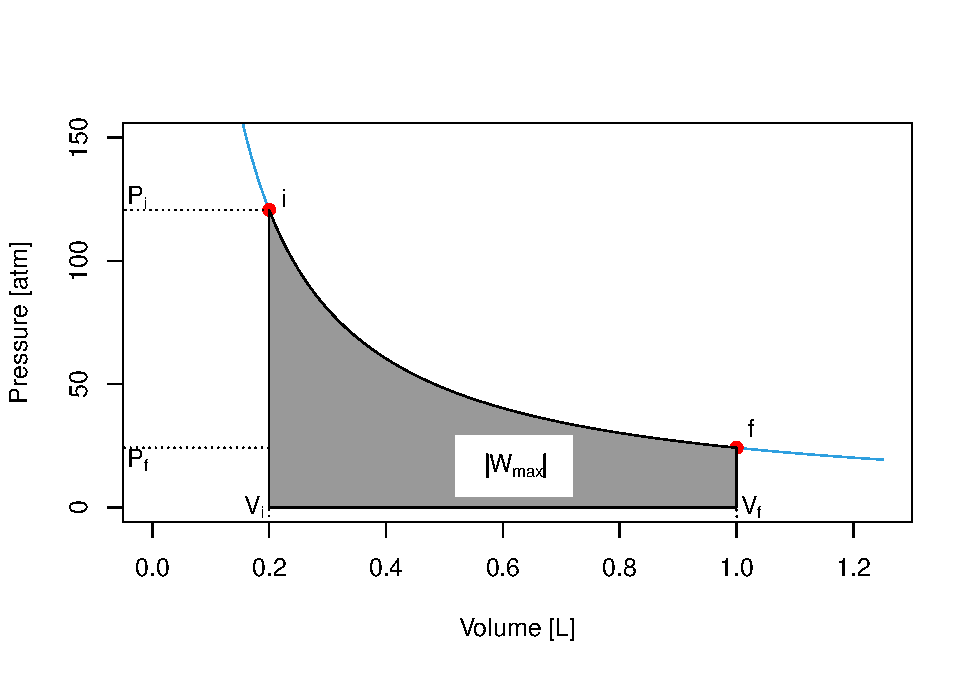
\includegraphics[width=0.5\linewidth,height=1\textheight]{pchem1_files/figure-latex/figures-side-4}

The integral on the right hand side of eq. \eqref{eq:WintsolvedV2} is similar to the integral that we already solved for eq. \eqref{eq:WintsolvedV}. Using the same trick, we can solve eq. \eqref{eq:WintsolvedV2} for an ideal gas as:

\begin{equation}
  \left| W_{\text{max}} \right| = nRT \int_{i}^{f} \frac{dV}{V} = nRT \ln \frac{V_f}{V_i}.
  \label{eq:WmaxV}
\end{equation}

This example demonstrates why work is a path function. If we perform a fast 1-step expansion, the system will perform an amount of work that is much smaller than the amount of work it can perform if the expansion between the same points happens slowly in an \(\infty\)-step process.

The same considerations that we made up to this point for expansion processes hold specularly for compression ones. The only difference is that the work associated with compressions will have a positive sign since it must be performed onto the system. As such, the amount of work for a transformation that happens in a finite amount of steps will be an upper bound to the minimum amount of work required to compress the system.\footnote{In contrast to a lower bound for expansion processes.} \(\left| W_{\text{min}} \right|\) for compressions is calculated as the area underneath the PV curve, exactly as \(\left| W_{\text{min}} \right|\) for expansions in eq. \eqref{eq:WintsolvedV2}.

\hypertarget{cycles-and-reversibility}{%
\subsection{Cycles and reversibility}\label{cycles-and-reversibility}}

Let's now consider the cycle in Figure \ref{fig:FigRevCyc}. The process in this case starts from state 1 (system at \(P_1V_1\)), expands to state 2 (system at \(P_2V_2\)), and compresses back to state 1 (system back to \(P_1V_1\)).

\begin{figure}

{\centering 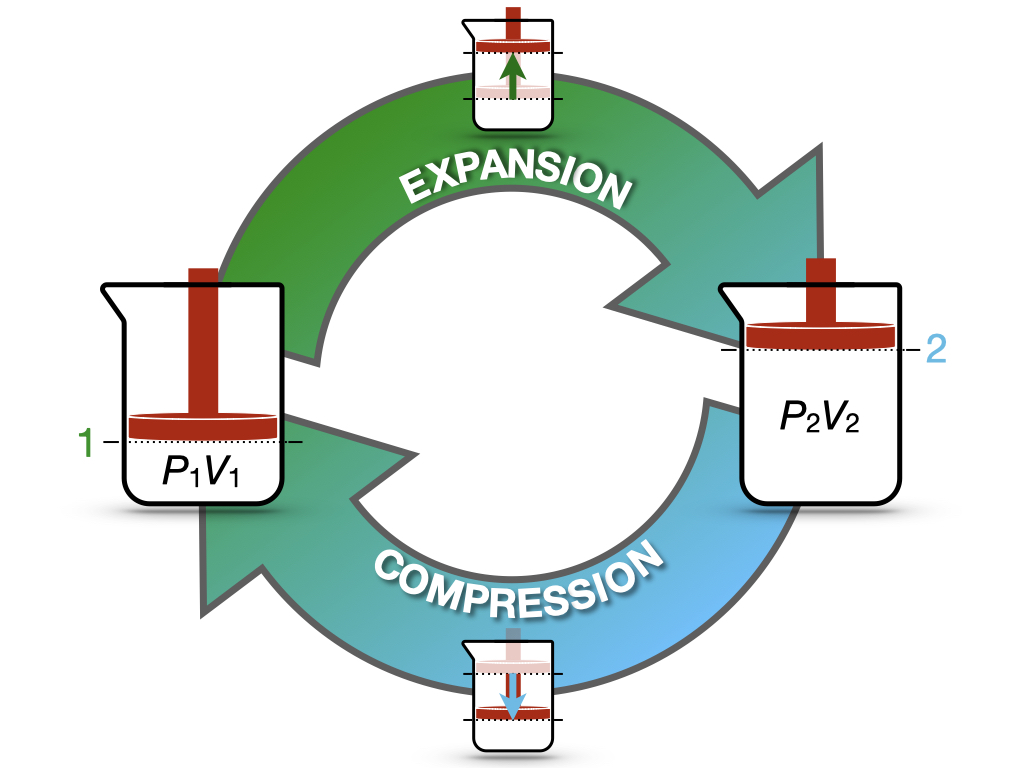
\includegraphics[width=0.8\linewidth]{./img/OEP_Figures.005} 

}

\caption{Expansion/Compression Cycle of an Ideal Gas.}\label{fig:FigRevCyc}
\end{figure}

Since the process starts and finishes at the same state, the value of the internal energy at the end of the process will be the same as its value at the beginning, regardless of the path:\footnote{recall that the internal energy is a state function, so its value depends exclusively from the conditions at the beginning and at the end. In a cycle, we're going back to the same point, so the conditions at the beginning and at the end are equal by definition.}

\begin{equation}
  \oint dU=0,
  \label{eq:de0}
\end{equation}

where the symbol \(\oint\) indicates an integral around a cycle. Considering the work associated with the cycle, however, the situation is radically different because it depends on the path that the system is taking, and in general
\begin{equation}
\oint_{\text{path}} đW \neq 0.
  \label{eq:dw0}
\end{equation}

For instance, if we perform the expansion in one step, the work associated with it will be (using eq. \eqref{eq:WintF}):\footnote{notice that the work for the expansion is negative, as it should be.}

\begin{equation}
  W^{\text{expansion}}_{\text{1-step}}=-P_2(\underbrace{V_2-V_1}_{>0})<0,
  \label{eq:Wexp1}
\end{equation}

and if we also perform the compression in 1-step:\footnote{notice that the work for the compression is positive, as it should be.}

\begin{equation}
  W^{\text{compression}}_{\text{1-step}}=-P_1(\underbrace{V_1-V_2}_{<0})>0.
  \label{eq:Wcomp1}
\end{equation}

With a little bit of math, it is easy to prove that the total work for the entire cycle is:

\begin{equation}
\begin{aligned}
W^{\text{cycle}}_{\text{1-step}} {} & =  W^{\text{expansion}}_{\text{1-step}}+W^{\text{compression}}_{\text{1-step}} \\
 & = -P_2(V_2-V_1)-P_1(V_1-V_2) \\
 & = -P_2(V_2-V_1)+P_1(V_2-V_1) \\
 & = (\underbrace{V_2-V_1}_{>0})(\underbrace{P_1-P_2}_{>0}) > 0,
\end{aligned}
  \label{eq:Wtot1}
\end{equation}

or, in other words, net work is destroyed.

\begin{quote}
In practice, if we want to manually perform this cycle by pushing on the piston by hand, we will notice that it requires more energy to push down than the amount it gives back when we release it, and it moves back up.
\end{quote}

In contrast, if both the expansion and the compression happen in a slow \(\infty\)-step manner, the work associated with them will be \(W_{\text{max}}\) and \(W_{\text{min}}\), respectively, which are calculated using eq. \eqref{eq:WmaxV}. The total work related with the cycle will be in this case:

\begin{equation}
\begin{aligned}
W^{\text{cycle}}_{\infty\text{-step}} {} & = W^{\text{expansion}}_{\text{max}}+W^{\text{compression}}_{\text{min}} \\
 & = -nRT \ln \frac{V_f}{V_i}-nRT \ln \frac{V_i}{V_f} \\
 & = -nRT \underbrace{\left( \ln \frac{V_f}{V_i} - \ln \frac{V_f}{V_i} \right) }_{=0}  = 0,
\end{aligned}
  \label{eq:Wtot2}
\end{equation}

which means that, in this case, work is not destroyed nor created.

\begin{quote}
In practice, if we were able to perform this cycle manually by pushing on the piston down by hand, we will notice that it requires the same amount of energy to push down than the amount it gives back when it moves up.
\end{quote}

This process can happen both ways without losses, and is called \emph{reversible}:

\begin{quote}
\begin{definition}
\protect\hypertarget{def:reversible}{}{\label{def:reversible} }\emph{Reversible process:} a process whose direction can be returned to its original position by inducing infinitesimal changes to some property of the system via its surroundings.\footnote{Definition from: Sears, F.W. and Salinger, G.L. (1986), Thermodynamics, Kinetic Theory, and Statistical Thermodynamics, 3rd edition (Addison-Wesley.)}
\end{definition}
\end{quote}

Reversible processes are ideal processes that are hard to realize in practice since they require transformations that happen in an infinite amount of steps (infinitely slowly).

\newcommand*{\standardstate}{{-\kern-6pt{\ominus}\kern-6pt-}}

\hypertarget{Thermochemistry}{%
\chapter{Thermochemistry}\label{Thermochemistry}}

\hypertarget{rxnenthalpy}{%
\section{Reaction Enthalpies}\label{rxnenthalpy}}

In the previous chapter, we have discussed thermodynamical changes in energy in the absence of chemical reactions. When a chemical reaction takes place, some bonds break and/or some new one form. This process either absorbs or releases the energy contained in these bonds. For a proper thermodynamic treatment of the system, this extra energy must be included in the net balance.

In this chapter, we will consider the heat associated with chemical reactions. Since most chemical reactions happen at constant atmospheric pressure (isobaric conditions) in the lab, we can use eq. \eqref{eq:dh2} to replace the inexact differential of the heat with the exact differential of the state function called enthalpy. The advantage of this transformation is that it allows us to study the heat associated with chemical reactions at constant pressure independently of their path. If we call the molecules at the beginning of the reaction ``reactants'' and the molecules at the end of the reaction ``products,'' the heat associated with the reaction (rxn) is defined as:

\begin{equation}
  \Delta_{\text{rxn}} H = H_{\text{products}}-H_{\text{reactants}} \; .
  \label{eq:DHrxn1}
\end{equation}

For example, if we take a simple reaction of the form:

\[ \mathrm{A} + \mathrm{B} \rightarrow \mathrm{C} + \mathrm{D}, \]

the heat at constant pressure is equal to the enthalpy of reaction, which is calculated as:

\begin{equation}
  Q_P = \Delta_{\text{rxn}} H = \underbrace{ \left (H_{\mathrm{C}}+H_{\mathrm{D}} \right) }_{\text{products}} - \underbrace{\left( H_{\mathrm{A}}+H_{\mathrm{B}}\right)}_{\text{reactants}}.
  \label{eq:DHrxn2}
\end{equation}

Using the chemistry sign convention, Definition \ref{def:chemistryconv}, reactions are classified in terms of the sign of their reaction enthalpies as follows:

\begin{quote}
\begin{definition}
\protect\hypertarget{def:exoendo}{}{\label{def:exoendo} }\(\;\)

\begin{itemize}
\tightlist
\item
  \(\Delta_{\text{rxn}} H > 0 \Rightarrow\) \emph{Endothermic reaction} (heat is gained by the system).
\item
  \(\Delta_{\text{rxn}} H < 0 \Rightarrow\) \emph{Exothermic reaction} (heat is lost by the system).
\end{itemize}
\end{definition}
\end{quote}

If we expand the sample reaction to account for its stoichiometry:

\[ a\mathrm{A} + b\mathrm{B} \rightarrow c\mathrm{C} + d\mathrm{D}\; , \]

where \(a,b,c,d\) are the stoichiometric coefficients of species \(\mathrm{A,B,C,D}\). Eq. \eqref{eq:DHrxn2} can be rewritten as:

\begin{equation}
  Q_P = \Delta_{\text{rxn}} H = \underbrace{\left( cH_{\mathrm{C}}+dH_{\mathrm{D}} \right) }_{\text{products}} - \underbrace{ \left( aH_{\mathrm{A}}+bH_{\mathrm{B}} \right)}_{\text{reactants}},
  \label{eq:DHrxn3}
\end{equation}

while for the most general case we can write it:

\begin{equation}
  \Delta_{\text{rxn}} H = \sum_i \nu_i H_i,
  \label{eq:DHrxn4}
\end{equation}

where \(\nu_i\) is the stoichiometric coefficient of species \(i\) with its own sign. The signs of the stoichiometric are defined according to eq. \eqref{eq:DHrxn3} as:

\begin{quote}
\begin{definition}
\protect\hypertarget{def:nui}{}{\label{def:nui} }\emph{Signs of the stoichiometric coefficients:}

\begin{itemize}
\tightlist
\item
  \(\nu_i\) is \textbf{positive} if \(i\) is a \textbf{product}.
\item
  \(\nu_i\) is \textbf{negative} if \(i\) is a \textbf{reactant}.
\end{itemize}
\end{definition}
\end{quote}

\hypertarget{formenthalpy}{%
\section{Standard Enthalpies of Formation}\label{formenthalpy}}

In principle, we could use eq. \eqref{eq:DHrxn3} to calculate the reaction enthalpy associated with any reaction. However, to do so, the absolute enthalpies \(H_i\) of reactants and products would be required. Unfortunately, absolute enthalpies are not known---and theoretically unknowable, since this would require an absolute zero for the enthalpy scale, which does not exist.\footnote{An example of a known absolute zero for a scale is the zero of the temperature scale, a temperature that can be approached only as a limit from above. No such thing exists for the enthalpy.} To prevent this problem, enthalpies relative to a defined reference state must be used. This reference state is defined at the constituent elements in their standard state, and the enthalpies of 1 mol of substance in this reference state are called \textbf{standard enthalpies of formation}.

\begin{quote}
\begin{definition}
\protect\hypertarget{def:stdenthapies}{}{\label{def:stdenthapies} }
The \emph{standard enthalpy of formation} of compound \(i\), \(\Delta_{\mathrm{f}} H_i^{-\kern-6pt{\ominus}\kern-6pt-}\), is the change of enthalpy during the formation of 1 mol of \(i\) from its constituent elements, with all substances in their standard states.
\end{definition}
\end{quote}

The standard pressure is defined at \(P^{{-\kern-6pt{\ominus}\kern-6pt-}} = 100 \; \mathrm{kPa} = 1 \; \mathrm{bar}\).\footnote{prior to 1982 the value of \(P^{{-\kern-6pt{\ominus}\kern-6pt-}} = 1.0 \mathrm{ atm}\) was used. The two values of \(P^{-\kern-6pt{\ominus}\kern-6pt-}\) are within 1\% of each other, since 1 atm = 101.325 kPa.} There is no standard temperature, but standard enthalpies of formation are usually reported at room temperature, \(T = 298.15 \; \mathrm{K}\). Standard states are indicated with the symbol \({-\kern-6pt{\ominus}\kern-6pt-}\) and they are defined for elements as the form in which such element is most stable at standard pressure (for example, for hydrogen, carbon, and oxygen the standard states are \(\mathrm{H}_{2(g)}, \mathrm{C}_{(s,\text{graphite})}, \text{and }\mathrm{O}_{2(g)}\), respectively).\footnote{There are some exception, such as phosphorus, for which the most stable form at 1 bar is black phosphorus, but white phosphorus is chosen as the standard reference state for zero enthalpy of formation. For the purposes of this course, however, we can safely ignore them.}

For example, the standard enthalpies of formation of some common compounds at \(T = 298.15 \; \mathrm{K}\) are calculated from the following reactions:

\begin{equation}
\begin{aligned}
  \mathrm{C}_{(s,\text{graphite})}+\mathrm{O}_{2(g)} \rightarrow \mathrm{CO}_{2(g)} \qquad & \Delta_{\mathrm{f}} H_{\mathrm{CO}_{2(g)}}^{-\kern-6pt{\ominus}\kern-6pt-}= -394 \; \text{kJ/mol} \\
   \mathrm{C}_{(s,\text{graphite})}+2 \mathrm{H}_{2(g)} \rightarrow \mathrm{CH}_{4(g)} \qquad & \Delta_{\mathrm{f}} H_{\mathrm{CH}_{4(g)}}^{-\kern-6pt{\ominus}\kern-6pt-}= -75 \; \text{kJ/mol} \\ 
   \mathrm{H}_{2(g)}+\frac{1}{2} \mathrm{O}_{2(g)} \rightarrow \mathrm{H}_2 \mathrm{O}_{(l)} \qquad & \Delta_{\mathrm{f}} H_{\mathrm{H}_2 \mathrm{O}_{(l)}}^{-\kern-6pt{\ominus}\kern-6pt-}= -286 \; \text{kJ/mol} 
\end{aligned}
\label{eq:someDfH}
\end{equation}

A comprehensive list of standard enthalpies of formation of inorganic and organic compounds is also reported in appendix \ref{appendix}.

\hypertarget{hessslaw}{%
\section{Hess's Law}\label{hessslaw}}

The calculation of a standard reaction enthalpy can be performed using the following cycle:

\begin{equation}
\begin{aligned}
 \text{reactants} & \quad \xrightarrow{\Delta_{\text{rxn}} H^{-\kern-6pt{\ominus}\kern-6pt-}} \quad \text{products} \\
\scriptstyle{-\Delta_{\text{f}} H_{\text{reactants}}^{-\kern-6pt{\ominus}\kern-6pt-}} \quad \bigg\downarrow \quad & \qquad \qquad \qquad \qquad \scriptstyle{\bigg\uparrow  \; \Delta_{\text{f}} H_{\text{products}}^{-\kern-6pt{\ominus}\kern-6pt-}} \\
 \text{"elements in } & \text{their standard reference state"}
\end{aligned}
\label{eq:Hesscycle}
\end{equation}

This process is summarized by the simple formula:

\begin{equation}
  \Delta_{\text{rxn}} H^{-\kern-6pt{\ominus}\kern-6pt-}= \Delta_{\mathrm{f}} H_{\text{products}}^{-\kern-6pt{\ominus}\kern-6pt-}- \Delta_{\mathrm{f}} H_{\text{reactants}}^{-\kern-6pt{\ominus}\kern-6pt-}.
  \label{eq:Hess1}
\end{equation}

Notice how there is a negative sign in front of the enthalpy of formation of the reactants because they are normally defined for the reactions that go from the elements to the reactants and not vice-versa. To close the cycle in eq. \eqref{eq:Hesscycle}, however, we should go from the reactants to the elements, and therefore we must invert the sign in front of the formation enthalpies of the reactants. Eq. \eqref{eq:Hess1} can be generalized using the same technique used to derive eq. \eqref{eq:DHrxn4}, resulting in:

\begin{equation}
  \Delta_{\text{rxn}} H^{-\kern-6pt{\ominus}\kern-6pt-}= \sum_i \nu_i \Delta_{\mathrm{f}} H_i^{-\kern-6pt{\ominus}\kern-6pt-},
  \label{eq:Hess}
\end{equation}

which is a mathematical expression of the law that is known as \textbf{Hess's Law}. Hess's law is valid at constant pressure because, at those conditions, the heat of reaction---a path function---is equal to the enthalpy of reaction---a state function. Therefore, the enthalpy of a reaction depends exclusively on the initial and final state, and it can be obtained via the pathway that passes through the elements in their standard state (the formation pathway).

\begin{quote}
\begin{exercise}
\protect\hypertarget{exr:HessLawEx}{}{\label{exr:HessLawEx} }Calculate the standard enthalpy of formation at 298 K for the combustion of 1 mol of methane, using the data in eq. \eqref{eq:someDfH}.

\emph{Solution:} The reaction that is under consideration is:
\begin{equation}
  \mathrm{CH}_{4(g)} + 2 \mathrm{O}_{2(g)} \rightarrow \mathrm{CO}_{2(g)} + 2 \mathrm{H}_2 \mathrm{O}_{(l)} \qquad \Delta_{\mathrm{f}} H_{\mathrm{CH}_{4(g)}}^{-\kern-6pt{\ominus}\kern-6pt-}= ?
\end{equation}

Using Hess's Law, \eqref{eq:Hess}, the enthalpy of formation for methane is:

\begin{equation}
 \Delta_{\text{rxn}} H^{-\kern-6pt{\ominus}\kern-6pt-}=  \Delta_{\text{f}} H^{-\kern-6pt{\ominus}\kern-6pt-}_{\mathrm{CO}_{2(g)}} + 2 \Delta_{\text{f}} H^{-\kern-6pt{\ominus}\kern-6pt-}_{\mathrm{H}_{2}O_{(l)}} - \Delta_{\text{f}} H^{-\kern-6pt{\ominus}\kern-6pt-}_{\mathrm{CH}_{4(g)}} - 2 \underbrace{\Delta_{\text{f}} H^{-\kern-6pt{\ominus}\kern-6pt-}_{\mathrm{O}_{2(g)}}}_{=0}
\end{equation}

whose values are reported in eqs. \eqref{eq:someDfH}. Notice that the formation enthalpy of \(O_{2(g)}\) is zero, since it is an element in its standard state. The final result is:

\begin{equation}
 \Delta_{\text{rxn}} H^{-\kern-6pt{\ominus}\kern-6pt-}=  \overbrace{-394}^{\Delta_{\text{f}} H^{-\kern-6pt{\ominus}\kern-6pt-}_{\mathrm{CO}_{2(g)}}} +2 \overbrace{(-286)}^{\Delta_{\text{f}} H^{-\kern-6pt{\ominus}\kern-6pt-}_{\mathrm{H}_{2}O_{(l)}}} - \overbrace{(-75)}^{\Delta_{\text{f}} H^{-\kern-6pt{\ominus}\kern-6pt-}_{\mathrm{CH}_{4(g)}}}  = -891 \mathrm{kJ/mol}.
\end{equation}

where the negative sign indicates that the reaction is exothermic (see \ref{def:exoendo}), as we should expect. The cycle that we used to solve this exercise can be summarized with :

\begin{equation}
\begin{aligned}
\mathrm{CH}_{4(g)} + & 2 \mathrm{O}_{2(g)} \quad \xrightarrow{\Delta_{\text{rxn}} H^{-\kern-6pt{\ominus}\kern-6pt-}} \quad \mathrm{CO}_{2(g)} + 2 \mathrm{H}_2 \mathrm{O}_{(l)} \\
  \scriptstyle{-\Delta_{\text{f}} H_{\mathrm{CH}_{4(g)},\mathrm{O}_{2(g)}}^{-\kern-6pt{\ominus}\kern-6pt-}} & \searrow \qquad \qquad \qquad \qquad \qquad \nearrow \; \scriptstyle{\Delta_{\text{f}} H_{\text{CO}_{2(g)},\mathrm{H}_{2(g)}}^{-\kern-6pt{\ominus}\kern-6pt-}}\\
  & \qquad \mathrm{H}_{2(g)}, \mathrm{C}_{s,\text{graphite}}, \mathrm{O}_{2(g)}
\end{aligned}
\end{equation}

Notice that at standard pressure and \(T = 298 \; \mathrm{K}\) water is in liquid form. However, when we burn methane, the heat associated with the exothermic reaction immediately vaporize the water. Substances in different states of matter have different formation enthalpies, and \(\Delta_{\text{f}} H^{-\kern-6pt{\ominus}\kern-6pt-}_{\mathrm{H}_{2}O_{(l)}} = -242 \  \mathrm{kJ/mol}\). The difference between the formation enthalpies of the same substance in different states represents the latent heat that separates them. For example, for water:

\begin{equation}
\begin{aligned}
\Delta_{\text{vap}} H^{-\kern-6pt{\ominus}\kern-6pt-}_{\mathrm{H}_2O} & = \Delta_{\text{f}} H^{-\kern-6pt{\ominus}\kern-6pt-}_{\mathrm{H}_{2}O_{(g)}} - \Delta_{\text{f}} H^{-\kern-6pt{\ominus}\kern-6pt-}_{\mathrm{H}_{2}O_{(l)}} \\
& = (-242) - (-286) = + 44 \; \text{kJ/mol}
\end{aligned}
\end{equation}

which is the latent heat of vaporization for water, \(\Delta_{\text{vap}} H^{-\kern-6pt{\ominus}\kern-6pt-}_{\mathrm{H}_2O}\). The latent heat is positive to indicate that the system absorbs energy in going from the liquid to the gaseous state (and it will release energy when going the opposite direction from gas to liquid).
\end{exercise}
\end{quote}

\hypertarget{calculations-of-enthalpies-of-reaction-at-t-neq-298-textk}{%
\section{\texorpdfstring{Calculations of Enthalpies of Reaction at \(T \neq 298 \; \text{K}\)}{Calculations of Enthalpies of Reaction at T \textbackslash neq 298 \textbackslash; \textbackslash text\{K\}}}\label{calculations-of-enthalpies-of-reaction-at-t-neq-298-textk}}

Standard enthalpies of formation are usually reported at room temperature (\(T\) = 298 K), but enthalpies of formation at any temperature \(T'\) can be calculated from the values at 298 K using eqs. \eqref{eq:Cpdef} and \eqref{eq:dh2}:

\begin{equation}
\begin{aligned}
dH = C_P dT \rightarrow & \int_{H_{T=298}^{-\kern-6pt{\ominus}\kern-6pt-}}^{H_{T'}} dH =  \int_{T=298}^{T'} C_P dT \\
            & H_{T'}^{-\kern-6pt{\ominus}\kern-6pt-}- H_{T=298}^{-\kern-6pt{\ominus}\kern-6pt-}= \int_{T=298}^{T'} C_P dT \\
            & H_{T'}^{-\kern-6pt{\ominus}\kern-6pt-}= H_{T=298}^{-\kern-6pt{\ominus}\kern-6pt-}+ \int_{T=298}^{T'} C_P dT,
\end{aligned}
  \label{eq:DrxnHneq298}
\end{equation}

which, in conjunction with Hess's Law (eq. \eqref{eq:Hess}), results in:

\begin{equation}
 \Delta_{\text{rxn}} H_{T'}^{-\kern-6pt{\ominus}\kern-6pt-}= \Delta_{\text{rxn}} H_{T=298}^{-\kern-6pt{\ominus}\kern-6pt-}+ \int_{T=298}^{T'} \Delta C_P dT,
  \label{eq:DrxnHneq298f}
\end{equation}

with \(\Delta C_P = \sum_i \nu_i C_{P,i}\).

\begin{quote}
\begin{exercise}
\protect\hypertarget{exr:DHtdiff298}{}{\label{exr:DHtdiff298} }Calculate \(\Delta_{\text{rxn}}H\) of the following reaction at 398 K, knowing that \(\Delta_{\text{rxn}}H^{-\kern-6pt{\ominus}\kern-6pt-}\) at 298 K is -283.0 kJ/mol, and the following \(C_P\) values: \(\mathrm{CO}_{(g)}\) = 29 J/(mol K), \(\mathrm{O}_{2(g)}\) = 30 J/(mol K), \(\mathrm{CO}_{2(g)}\) = 38 J/(mol K):

\[
\mathrm{CO}_{(g)}+\frac{1}{2}\mathrm{O}_{2(g)} \rightarrow \mathrm{CO}_{2(g)},
\]

\emph{Solution:} Using eq. \eqref{eq:DrxnHneq298f} we obtain:

\[
 \Delta_{\text{rxn}} H^{398} = \overbrace{-283.0}^{\Delta_{\text{rxn}}H^{-\kern-6pt{\ominus}\kern-6pt-}} + \int_{298}^{398} ( \overbrace{38}^{C_P^{\mathrm{CO}_2}} -\overbrace{29}^{C_P^{\mathrm{CO}}} -\frac{1}{2}\overbrace{30}^{C_P^{\mathrm{O}_2}} ) \times 10^{3} dT,
\]

which, assuming that the heat capacities does not depend on the temperature, becomes:

\begin{equation}
\begin{aligned}
 \Delta_{\text{rxn}} H^{398} &= -283.0 + \left(38-29-\frac{1}{2}30 \right) \times 10^{-3} (398-298) \\ &= -283.6 \; \text{kJ/mol}.
\end{aligned}
\end{equation}

As we notice from this result, a difference in temperature of 100 K translates into a change in \(\Delta_{\text{rxn}}H^{-\kern-6pt{\ominus}\kern-6pt-}\) of this reaction of only 0.6 kJ/mol. This is a trend that is often observed, and values of \(\Delta_{\text{rxn}}H\) are very weakly dependent on changes in temperature for most chemical reactions. This numerical result can also be compared with the amount that is experimentally measured for \(\Delta_{\text{rxn}}H^{398}\) of this reaction, which is --283.67 kJ/mol. This comparison strongly supports the assumption that we used to solve the integral in eq. \eqref{eq:DrxnHneq298f}, confirming that the heat capacities are mostly independent of temperature.
\end{exercise}
\end{quote}

\hypertarget{ThermodynamicCycles}{%
\chapter{Thermodynamic Cycles}\label{ThermodynamicCycles}}

The first law of thermodynamics places no restrictions on the conversion of energy from one form to another. For example, let's consider once again the Joule experiment (Figure \ref{fig:FigJexp}). If we design a cycle that goes from the gas on the left chamber only to the gas equilibrated in both chambers and backward, as in Figure \ref{fig:FigJexpC}, there are no restrictions imposed on this hypothetical cycle by the first law.

\begin{figure}

{\centering 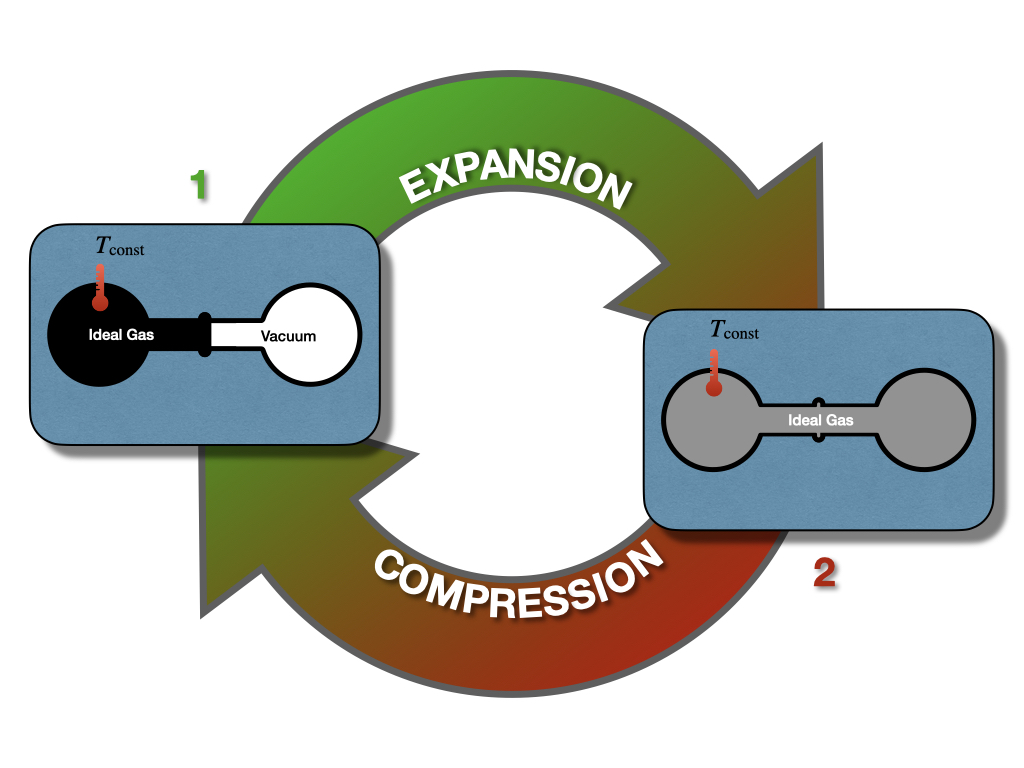
\includegraphics[width=0.8\linewidth]{./img/OEP_Figures.008} 

}

\caption{Closing the Cycle in The Joule Expansion Experiment.}\label{fig:FigJexpC}
\end{figure}

As we saw in section \ref{isothermalE}, states 1 and 2 have exactly the same energy at constant temperature. Restricting the analysis to the information contained in the first law, the ideal gas could hypothetically go from state 1 (all gas in the left chamber) to state 2 (gas in both chambers), as well as spontaneously close the cycle back from state 2 to state 1, without external intervention. While the transformation from 1 \(\rightarrow\) 2 is intuitively spontaneous (it's the same transformation that we considered in section \ref{isothermalE}), the backward transformation from 2 \(\rightarrow\) 1 is clearly not as intuitive. In this case, the gas should spontaneously compress back to the left side, leaving a vacuum on the right chambers, without interventions from the outside. This transformation is clearly never observed. A gas just does not spontaneously concentrate on one side of a room, leaving a vacuum on the other side. In fact, when we need to create a vacuum, a lot of energy must be spent. Suppose we use exclusively information contained in the first law. In this case, there is nothing that might suggest a system's preference to perform the transformation 1 \(\rightarrow\) 2, while restricting the 2 \(\rightarrow\) 1 from happening spontaneously. Both states have the same energy, and

\begin{equation}
  \oint dU=0,
  \label{eq:de0c}
\end{equation}

James Joule himself was indeed convinced that this must be the case and that we don't observe the backward transformation in practice only because we cannot build ideal machines.\footnote{Either because we don't really have ideal gases, or because we are unable to construct mechanical devices without loss, or in general because of other experimental factors} Another scientist of that era was not convinced. William Thomson, the 1\textsuperscript{st} Baron Kelvin (1824--1907), was unsure about this idea, and invested substantial resources to try to prove Joule's wrong.\footnote{Interestingly enough, both Joule and Lord Kelvin are now recognized as key figures in the development of thermodynamics and science in general. So much so, that the energy unit and the temperature unit in the SI system are named after them.}

A few years later, the controversy between Joule and Kelvin was redeemed in favor of the latter, thanks to the experiments of French military engineer Nicolas Léonard Sadi Carnot (1796--1832). The work of Carnot began in France several years before Joule and Kelvin's time.\footnote{Carnot's lone book, the \href{https://en.wikipedia.org/wiki/Reflections_on_the_Motive_Power_of_Fire}{\emph{Réflexions sur la Puissance Motrice du Feu} (``Reflections on the Motive Power of Fire'')} was published in France in 1824, the same year Kelvin was born and just 6 years after Joule's birth.} At that time, the importance of steam engines was growing for industrial applications, but a theoretical perspective was lacking. Carnot was convinced that a scientific understanding of heat engines was necessary to improve their efficiency.

\hypertarget{carnotcyclesect}{%
\section{Carnot Cycle}\label{carnotcyclesect}}

The main contribution of Carnot to thermodynamics is his abstraction of the steam engine's essential features into a more general and idealized heat engine. The definition of Carnot's idealized cycle is as follows:

\begin{quote}
\begin{definition}
\protect\hypertarget{def:carnotcycle}{}{\label{def:carnotcycle} }
A \emph{Carnot cycle} is an idealized process composed of two isothermal and two adiabatic transformations. Each transformation is either an expansion or a compression of an \emph{ideal gas}. All transformations are assumed to be \emph{reversible}, and no energy is lost to mechanical friction.
\end{definition}
\end{quote}

A Carnot cycle connects two ``heat reservoirs'' at temperatures \(T_h\) (hot) and \(T_l\) (low), respectively. The reservoirs have a large thermal capacity so that their temperatures are unaffected by the cycle. The system is composed exclusively by the ideal gas, which is the only substance that changes temperature throughout the cycle. If we report the four transformations of a Carnot cycle on a \(PV\) diagram, we obtain the following plot:

\begin{figure}

{\centering 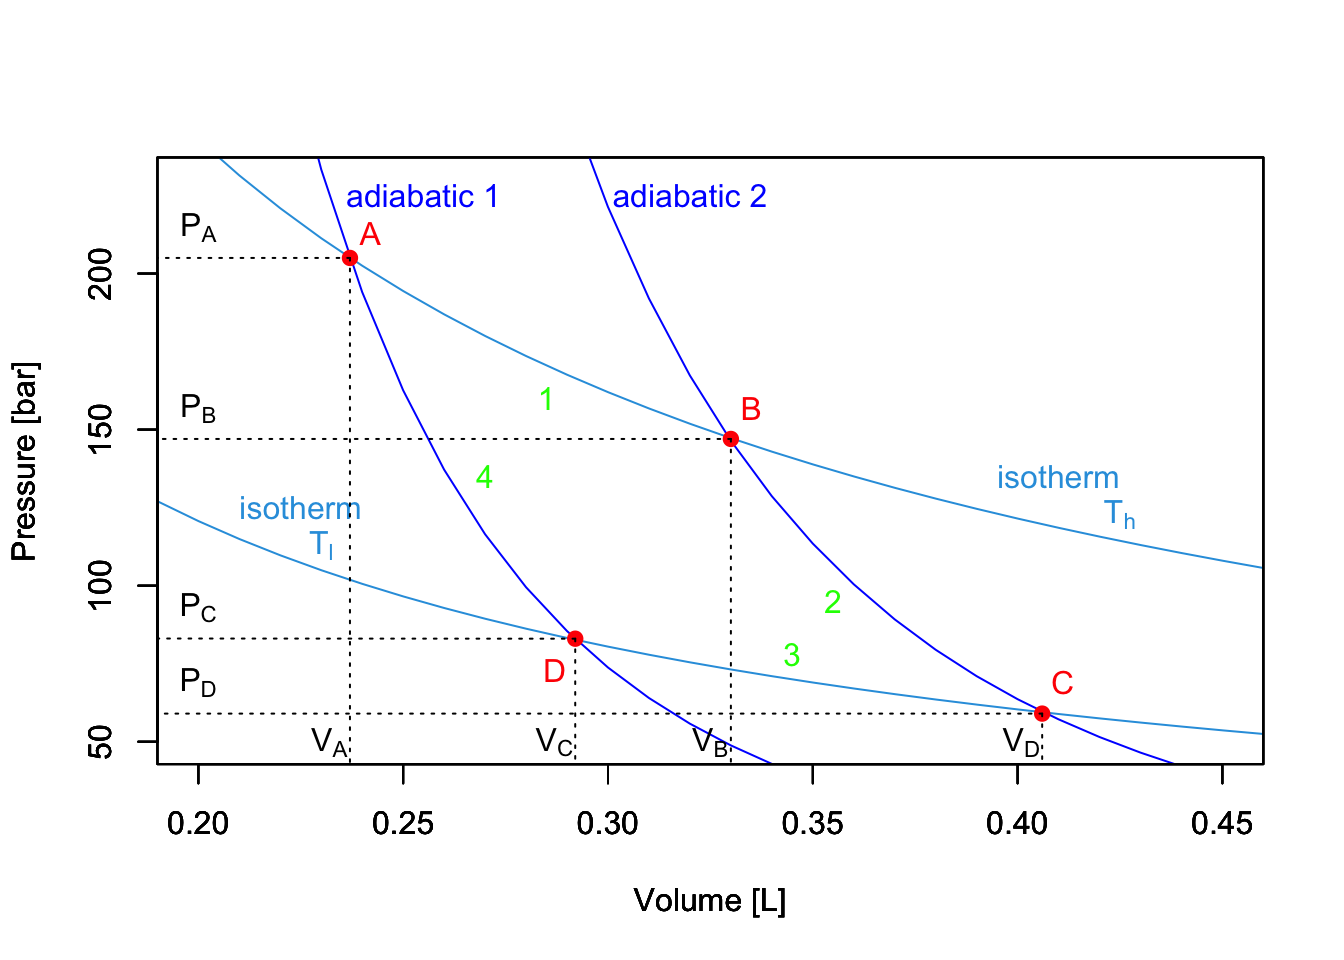
\includegraphics[width=0.7\linewidth]{pchem1_files/figure-latex/FigCarnotPV-1} 

}

\caption{PV-Diagram of a Carnot Cycle.}\label{fig:FigCarnotPV}
\end{figure}

\hypertarget{CCstage1}{%
\subsection{\texorpdfstring{Stage 1: isothermal expansion \(A \rightarrow B\)}{Stage 1: isothermal expansion A \textbackslash rightarrow B}}\label{CCstage1}}

\begin{center}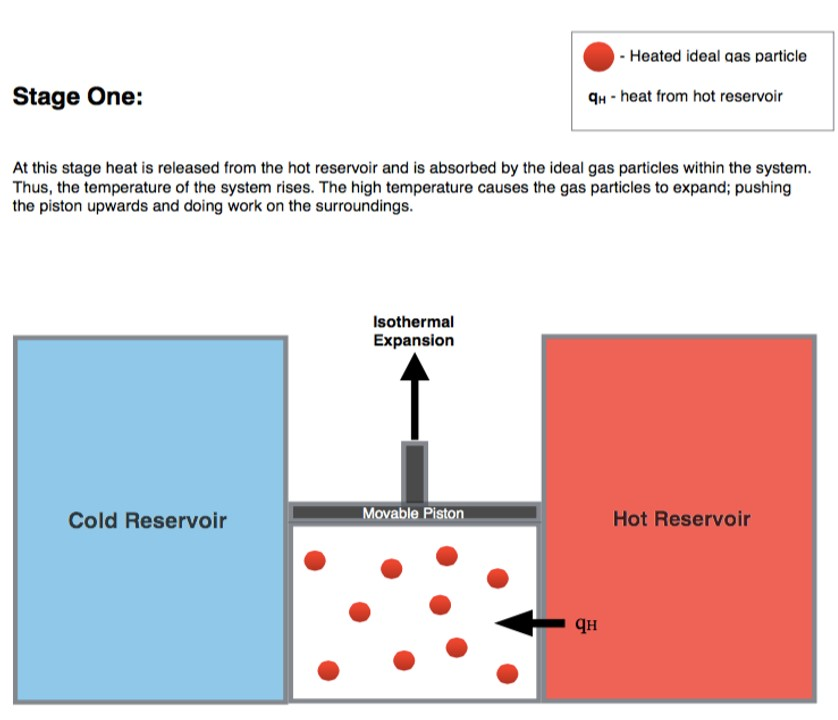
\includegraphics[width=0.7\linewidth]{./img/OEP_Figures.007a} \end{center}

Starting the analysis of the cycle from point \(A\) in Figure \ref{fig:FigCarnotPV},\footnote{The stages of a Carnot depicted at the beginning of each of this section and the following three ones are genetaken from \href{https://en.wikipedia.org/wiki/Carnot_cycle}{Wikipedia}, and have been generated and distributed by Author BlyumJ under CC-BY-SA license.} the first transformation we encounter is an isothermal expansion at \(T_h\). Since the transformation is isothermal:

\begin{equation}
U_1 = \overbrace{W_1}^{<0} + \overbrace{Q_1}^{>0} = 0 \Rightarrow Q_1 = -W_1,
  \label{eq:CCst1}
\end{equation}

and heat and work can be calculated for this stage using either eqs. \eqref{eq:WintsolvedV} or \eqref{eq:WintsolvedP}:

\begin{equation}
\begin{aligned}
 Q_1 & = \left| Q_h \right|  = nRT_h \overbrace{\ln \frac{V_B}{V_A}}^{>0 \text{ since } V_B>V_A} > 0, \\
 W_1 & = -Q_1 = - nRT_h \ln \frac{V_B}{V_A} < 0,
\end{aligned}
  \label{eq:CCst1b}
\end{equation}

where we denoted \(\left| Q_h \right|\) the absolute value of the heat that gets \textbf{into} the system from the hot reservoir.

\hypertarget{CCstage2}{%
\subsection{\texorpdfstring{Stage 2: adiabatic expansion \(B \rightarrow C\)}{Stage 2: adiabatic expansion B \textbackslash rightarrow C}}\label{CCstage2}}

\begin{center}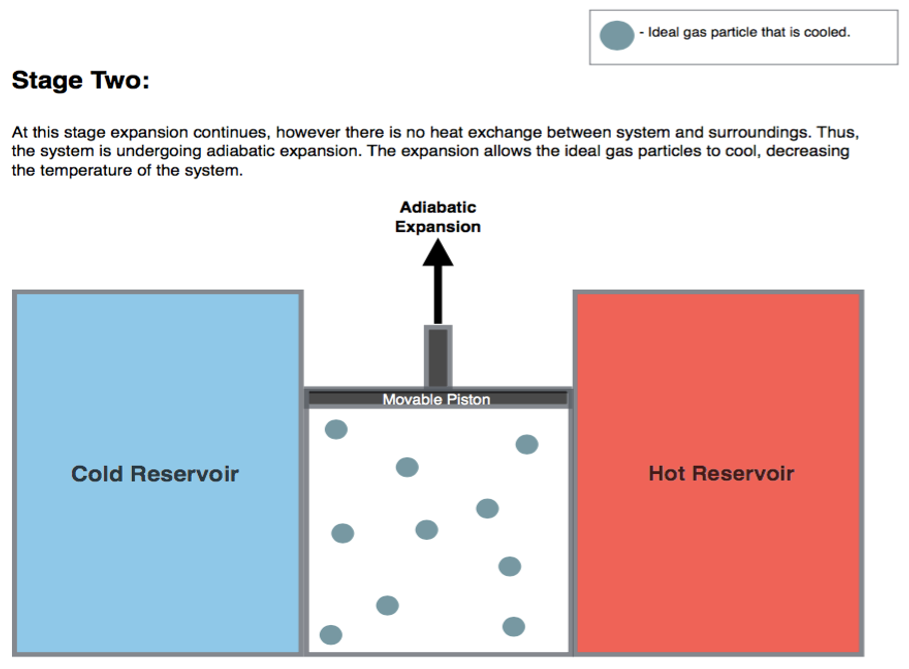
\includegraphics[width=0.7\linewidth]{./img/OEP_Figures.007b} \end{center}

The second transformation is an adiabatic expansion between \(T_h\) and \(T_l\). Since we are at adiabatic conditions:

\begin{equation}
Q_2 = 0 \Rightarrow U_2 = W_2,
  \label{eq:CCst2}
\end{equation}

and the negative energy (expansion work) can be calculated using:

\begin{equation}
U_2 = W_2 = n \underbrace{\int_{T_h}^{T_l} C_V dT}_{<0 \text{ since } T_\mathrm{l}<T_\mathrm{h}} < 0.
  \label{eq:CCst2b}
\end{equation}

\hypertarget{CCstage3}{%
\subsection{\texorpdfstring{Stage 3: isothermal compression \(C \rightarrow D\)}{Stage 3: isothermal compression C \textbackslash rightarrow D}}\label{CCstage3}}

\begin{center}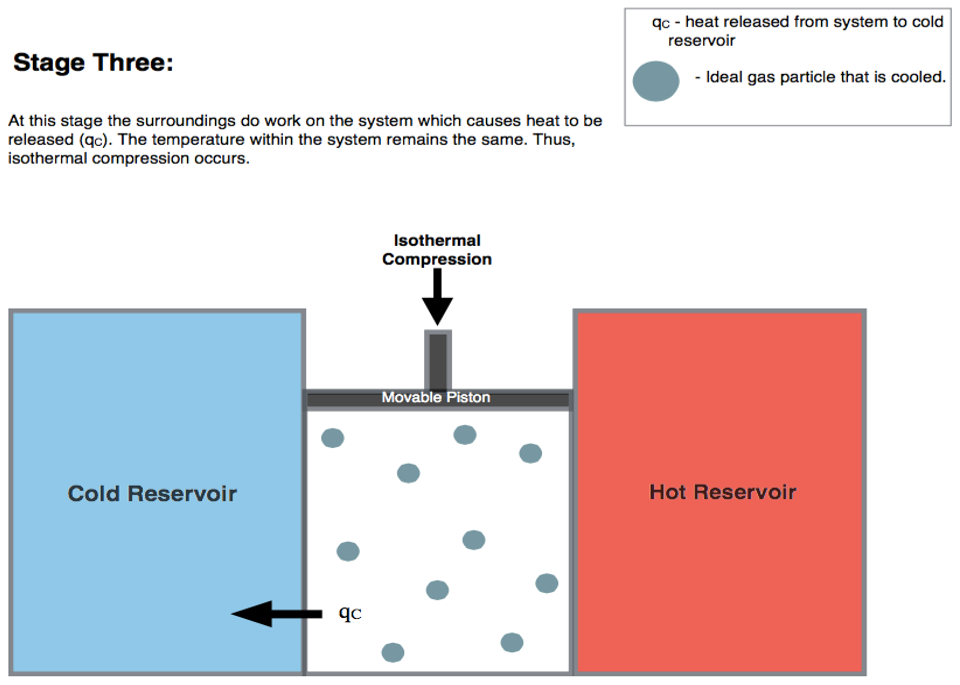
\includegraphics[width=0.7\linewidth]{./img/OEP_Figures.007c} \end{center}

The third transformation is an isothermal compression at \(T_l\). The formulas are the same as those used for stage 1, but they will results in heat and work with reversed signs (since this is a compression):

\begin{equation}
U_3 = \overbrace{W_3}^{>0} + \overbrace{Q_3}^{<0} = 0 \Rightarrow Q_3 = -W_3,
  \label{eq:CCst3}
\end{equation}

and:

\begin{equation}
\begin{aligned}
 Q_3 & = \left| Q_l \right|  = nRT_l \overbrace{\ln \frac{V_D}{V_C}}^{<0 \text{ since } V_D<V_C} < 0 , \\
 W_3 & = -Q_3 = - nRT_l \ln \frac{V_D}{V_C} > 0,
\end{aligned}
  \label{eq:CCst3b}
\end{equation}

where \(\left| Q_l \right|\) is the absolute value of the heat that gets \textbf{out of} the system to the cold reservoir (\(\left| Q_l \right|\) being the heat entering the system).

\hypertarget{CCstage4}{%
\subsection{\texorpdfstring{Stage 4: adiabatic compression \(D \rightarrow A\)}{Stage 4: adiabatic compression D \textbackslash rightarrow A}}\label{CCstage4}}

\begin{center}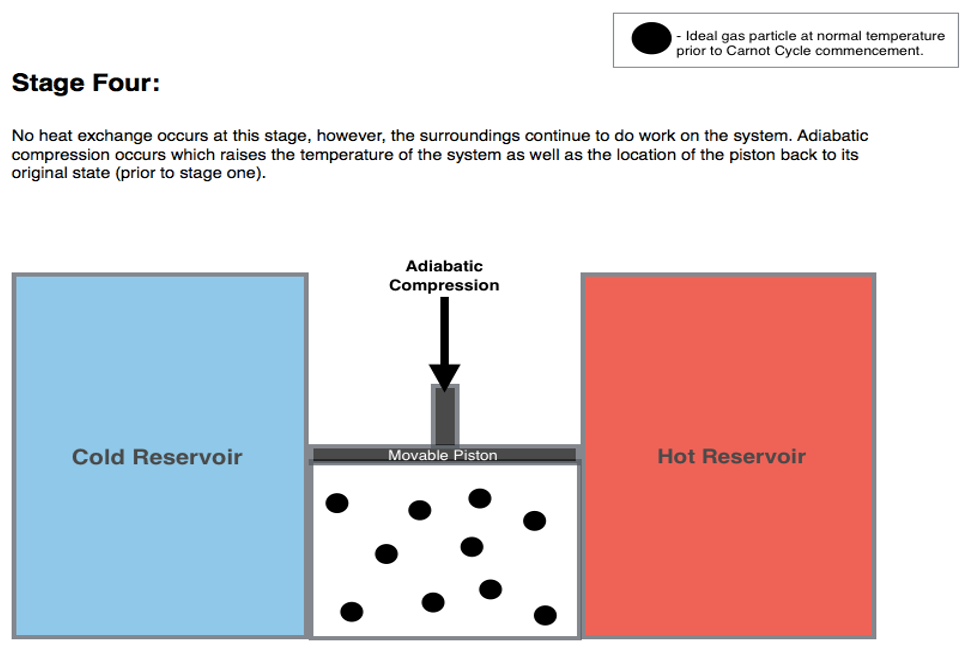
\includegraphics[width=0.7\linewidth]{./img/OEP_Figures.007d} \end{center}

The fourth and final transformation is an adiabatic comprssion that restores the system to point \(A\), bringing it from \(T_l\) to \(T_h\). Similarly to stage 3:

\begin{equation}
Q_4 = 0 \Rightarrow U_4 = W_4,
  \label{eq:CCst4}
\end{equation}

Since we are at adiabatic conditions. The energy associated with this process is now positive (compression work), and can be calculated using:

\begin{equation}
U_4 = W_4 = n \underbrace{\int_{T_l}^{T_h} C_V dT}_{>0 \text{ since } T_\mathrm{h}>T_\mathrm{l}} > 0.
  \label{eq:CCst4b}
\end{equation}

Notice how \(U_4 = -U_2\) because \(\int_x^y=-\int_y^x\).

\hypertarget{UWQCarnot}{%
\section{Energy, Heat, and Work in the Carnot Cycle}\label{UWQCarnot}}

Summarizing the results of the previous sections, the total amount of energy for a Carnot cycle is:

\begin{equation}
\begin{aligned}
  U_{\text{TOT}} & = U_1+U_2+U_3+U_4 \\
                 & = 0 + n \int_{T_h}^{T_l} C_V dT + 0 + n \int_{T_l}^{T_h} C_V dT  \\
                 & = n \int_{T_h}^{T_l} C_V dT - n \int_{T_h}^{T_l} C_V dT = 0 \\
\end{aligned}
  \label{eq:UtotCC}
\end{equation}

which is obviously zero, since \(\oint dU=0\). The amounts of work and heat, however, are not zero, since \(Q\) and \(W\) are path functions. Therefore:

\begin{equation}
\begin{aligned}
  W_{\text{TOT}} & = W_1+W_2+W_3+W_4 \\
                 & = - nRT_h \ln \frac{V_B}{V_A} + n \int_{T_h}^{T_l} C_V dT - nRT_l \ln \frac{V_D}{V_C} + n \int_{T_l}^{T_h} C_V dT \\
                 & = nRT_h \ln \frac{V_B}{V_A} + nRT_l \ln \frac{V_D}{V_C}, \\
\end{aligned}
  \label{eq:WtotCC}
\end{equation}

which, considering that \(V_C/V_D=V_B/V_A\), reduces to:

\begin{equation}
  W_{\text{TOT}} = - nR \left( T_h-T_l \right) \ln \frac{V_B}{V_A} < 0,
  \label{eq:WtotCC2}
\end{equation}

which is negative, because \(T_h>T_l\) and \(V_B>V_A\). Negative work means that the work is done by the system. In other words, the system is performing \(PV\)-work by transferring heat from a hot reservoir to a cold one via a Carnot cycle. On the other hand, for the heat:

\begin{equation}
\begin{aligned}
  Q_{\text{TOT}} & = Q_1+Q_2+Q_3+Q_4 \\
                 & = Q_h + 0 + Q_l + 0    \\
                 & = nRT_h \ln \frac{V_B}{V_A} + nRT_l \ln \frac{V_D}{V_C} \\
                 & = nR \left( T_h-T_l \right) \ln \frac{V_B}{V_A} = -W_{\text{TOT}},
\end{aligned}
  \label{eq:QtotCC}
\end{equation}

which, simplifies to:

\begin{equation}
W_{\text{TOT}}=-(Q_1+Q_3),
  \label{eq:WtotCC3}
\end{equation}

and, replacing \(Q_1\) and \(Q_3\) with the absolute values of the heats drawn from the hot and cold reservoirs, \(\left| Q_h \right|\), and \(\left| Q_l \right|\) respectively:

\begin{equation}
\left| W_{\text{TOT}} \right| = \left| Q_h \right| - \left| Q_l \right|,
  \label{eq:QtotCC2}
\end{equation}

or, in other words, more heat is extracted from the hot reservoir than it is put into the cold one. The difference between the absolute value of these amounts of heat gives the total work of the cycle. This process is depicted in Figure \ref{fig:FigCarnotEff}.

\begin{figure}

{\centering 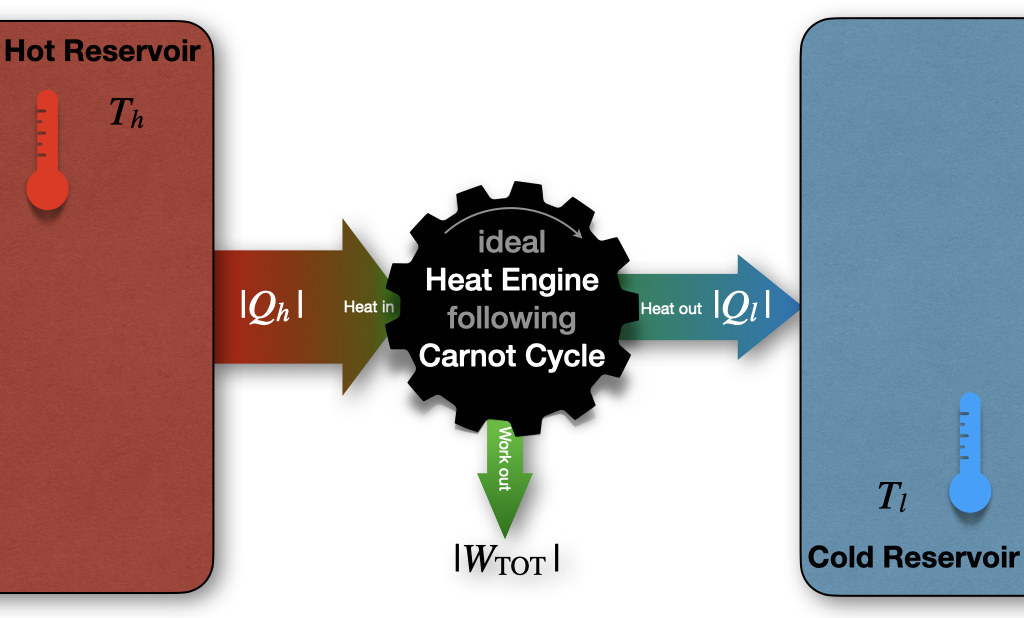
\includegraphics[width=0.8\linewidth]{./img/OEP_Figures.009} 

}

\caption{Carnot Cycle Diagram.}\label{fig:FigCarnotEff}
\end{figure}

\begin{quote}
\begin{exercise}
\protect\hypertarget{exr:CarnotEx}{}{\label{exr:CarnotEx} }Up to this point, we have discussed Carnot cycles working in the hot \(\rightarrow\) cold direction (\(A\) \(\rightarrow\) \(B\) \(\rightarrow\) \(C\) \(\rightarrow\) \(D\) \(\rightarrow\) \(A\)), since this is the primary mode of operation of heat engines that produce work. However, a heat engine could also---in principle---work in the reversed cold \(rightarrow\) hot direction (\(A\) \(\rightarrow\) \(D\) \(\rightarrow\) \(C\) \(\rightarrow\) \(B\) \(\rightarrow\) \(A\)). Write the equations for heat, work, and energy of each stage of a Carnot cycle going the opposite direction than the one discussed in sections \ref{carnotcyclesect} and \ref{UWQCarnot}.

\emph{Solution:} When the heat engine works in reverse order, the formulas remain the same, but all the signs in front of \(Q\), \(W\), and \(U\) will be reversed. In this case, the total work would get \textbf{into} the systems, and heat would be transferred from the cold reservoir to the hot one. Figure \ref{fig:FigCarnotEff} would be modified as:
\end{exercise}
\end{quote}

\begin{flushright}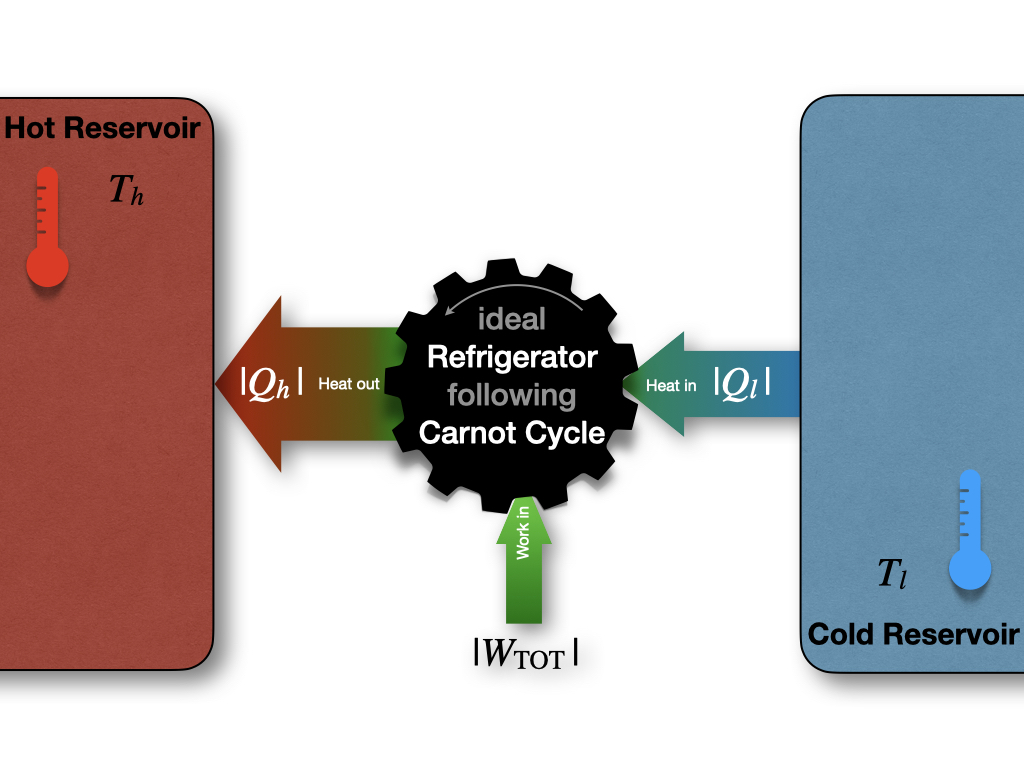
\includegraphics[width=0.6\linewidth]{./img/OEP_Figures.010} \end{flushright}

This reversed mode of operation is the basic principle behind refrigerators and air conditioning.

\hypertarget{efficiency-of-a-carnot-cycle}{%
\section{Efficiency of a Carnot Cycle}\label{efficiency-of-a-carnot-cycle}}

The efficiency (\(\varepsilon\)) of a cycle is defined as the ratio between the absolute value of the work extracted from the cycle (\(\left| W_{\text{TOT}} \right|\)) and the heat that gets into the system (\(\left| Q_h \right|\)):

\begin{equation}
\varepsilon = \frac{\left| W_{\text{TOT}} \right|}{\left| Q_h \right|} =\frac{-W_{\text{TOT}}}{Q_1}
\label{eq:effCC1}
\end{equation}

where the minus sign in front of the work is necessary because the efficiency is defined as a positive number. Replacing eq. \eqref{eq:WtotCC3} into \eqref{eq:effCC1}, we obtain:

\begin{equation}
\varepsilon = \frac{Q_3+Q_1}{Q_1} = 1+\frac{Q_3}{Q_1}.
\label{eq:effCC2}
\end{equation}

If we go back to eq. \eqref{eq:effCC1} and we replace eq. \eqref{eq:WtotCC2} for \(W_{\mathrm{TOT}}\) and eq. \eqref{eq:CCst1b} for \(Q_1\), we obtain:

\begin{equation}
\varepsilon = \frac{nR \left( T_h - T_l \right) \ln V_B/V_A}{nRT_h \ln V_B/V_A} = \frac{T_h-T_l}{T_h}=1-\frac{T_l}{T_h }<1,
\label{eq:effCC3}
\end{equation}

which proves that the efficiency of a Carnot cycle is strictly smaller than 1.\footnote{Eq. \eqref{eq:effCC3} can be equal to 1 only if \(T_l=0 \; \text{K}\) or \(T_h=\infty\), two conditions that are both equally impossible.} In other words, no cycle can convert 100\% of the heat into work it extracts from a hot reservoir. This finding had remarkable consequences on the entire thermodynamics field and set the foundation for the introduction of entropy. We will use eqs. \eqref{eq:effCC1} and \eqref{eq:effCC3} for this purpose in the next chapter, but we conclude the discussion on Carnot cycles by returning back to Lord Kelvin. In 1851 he used this finding to state his statement ``It is impossible for a self-acting machine, unaided by any external agency, to convey heat from one body to another at a higher temperature. It is impossible, by means of inanimate material agency, to derive mechanical effect from any portion of matter by cooling it below the temperature of the coldest of the surrounding objects.''\footnote{Thomson W. \href{https://www.biodiversitylibrary.org/item/126047\#page/295/mode/1up}{Transactions of the Royal Society of Edinburgh. 1851 XX 261--268, 289--298.}.} This statement conclusively disproved Joule's original theories and demonstrated that there is some fundamental principle to govern the flow of heat beyond the first law of thermodynamics.

\hypertarget{SecondLaw}{%
\chapter{Second Law of Thermodynamics}\label{SecondLaw}}

In the previous chapter, we have discussed heat engines as a means of understanding how some processes are spontaneous while others are not. Carnot's findings did not just simply inspire Lord Kelvin on this subject, but they also motivated Rudolf Clausius (1822--1888) to introduce the concept of entropy.

\hypertarget{entropyint}{%
\section{Entropy}\label{entropyint}}

Let's return to the definition of efficiency of a Carnot cycle and bring together eqs. \eqref{eq:effCC2} and \eqref{eq:effCC3}:

\begin{equation}
\varepsilon = 1+\frac{Q_3}{Q_1} = 1-\frac{T_l}{T_h}.
\label{eq:effcQT}
\end{equation}

Simplifying this equality, we obtain:

\begin{equation}
\frac{Q_3}{T_l} = -\frac{Q_1}{T_h},
\label{eq:effcQTrearr}
\end{equation}

or alternatively:

\begin{equation}
\frac{Q_3}{T_l} + \frac{Q_1}{T_h} = 0.
\label{eq:effcQTrearr2}
\end{equation}

The left hand side of eq. \eqref{eq:effcQTrearr2} contains the sum of two quantities around the Carnot cycle, each calculated as \(\frac{Q_{\mathrm{REV}}}{T}\), with \(Q_{\mathrm{REV}}\) being the heat exchanged at reversible conditions (recall that according to Definition \ref{def:carnotcycle} each transformation in a Carnot cycle is reversible). Eq. \eqref{eq:effcQTrearr} can be generalized to a sequence of connected Carnot cycles joining more than two isotherms by taking the summation across different temperatures:

\begin{center}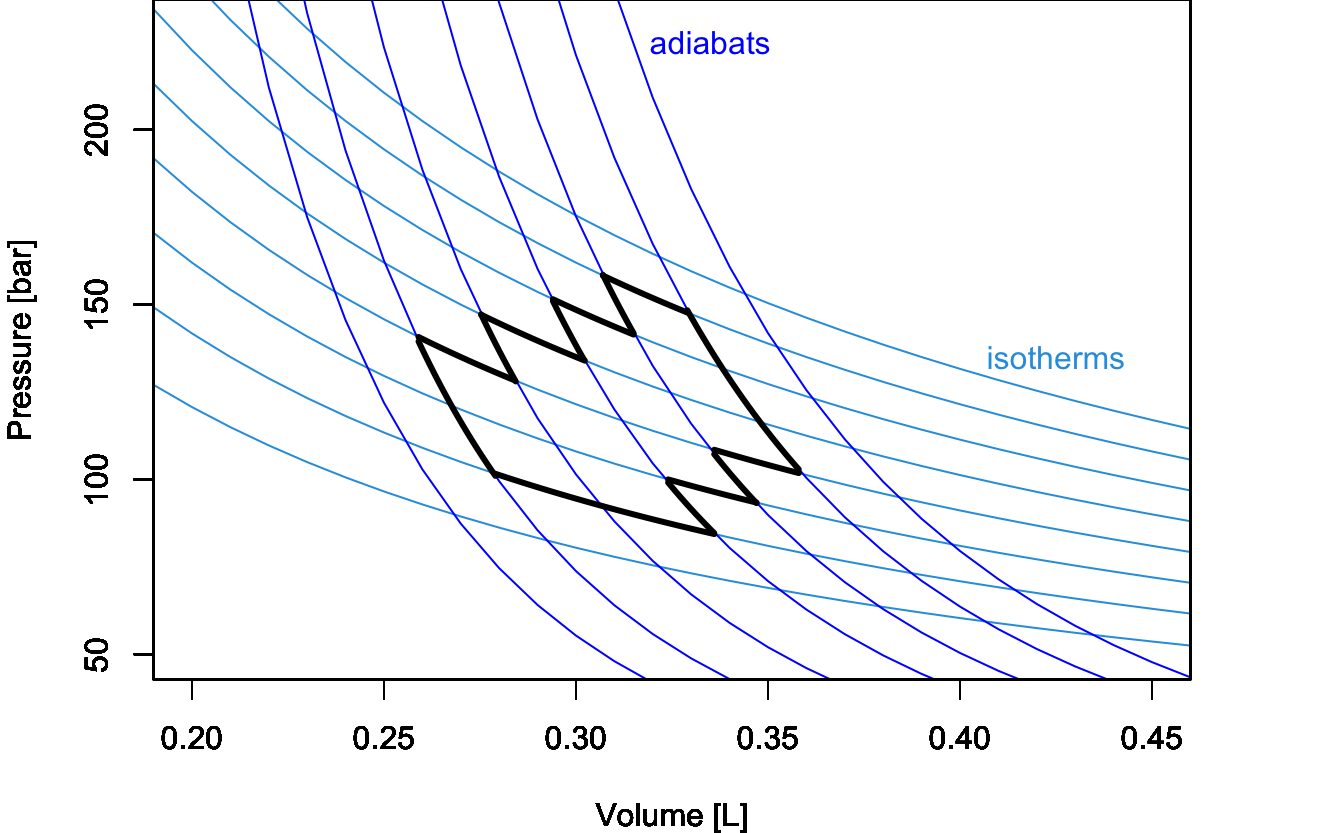
\includegraphics[width=0.7\linewidth]{pchem1_files/figure-latex/unnamed-chunk-12-1} \end{center}

\begin{equation}
\sum_i \frac{Q_{\mathrm{REV}}}{T_i} = 0,
\label{eq:effQrevT}
\end{equation}

where the summation happens across a sequence of Carnot cycles that connects different temperatures. Eqs. \eqref{eq:effcQTrearr2} and \eqref{eq:effQrevT} show that for a Carnot cycle---or a series of connected Carnot cycles---there exists a conserved quantity obtained by dividing the heat associated with each reversible stage and the temperature at which such heat is exchanged. If a quantity is conserved around a cycle, it must be independent on the path, and therefore it is a state function. Looking at similar equations, Clausius introduced in 1865 a new state function in thermodynamics, which he decided to call entropy and indicate with the letter \(S\):

\begin{quote}
\begin{definition}
\protect\hypertarget{def:entropy}{}{\label{def:entropy} }\emph{Entropy:} \begin{equation}
S = \frac{Q_{\mathrm{REV}}}{T}.
\end{equation}
\end{definition}
\end{quote}

We can use the new state function to generalize eq. \eqref{eq:effQrevT} to any reversible cycle in a \(PV\)-diagram by using the rules of calculus. First, we will slice \(S\) into an infinitesimal quantity:

\begin{equation}
dS = \frac{đQ_{\mathrm{REV}}}{T},
\label{eq:dentropy}
\end{equation}

then we can extend the summation across temperatures of eq. \eqref{eq:effQrevT} to a sum over infinitesimal quantities---that is the integral---around the cycle:

\begin{equation}
\oint dS = \oint \frac{đQ_{\mathrm{REV}}}{T} = 0.
\label{eq:ds0}
\end{equation}

\hypertarget{irreversible-cycles}{%
\section{Irreversible Cycles}\label{irreversible-cycles}}

Up to this point, we have discussed \emph{reversible} cycles only. Notice that the heat that enters the definition of entropy (Definition \ref{def:entropy} is the heat exchanged at reversible conditions since it is only at those conditions that the right-hand side of eq. \eqref{eq:dentropy} becomes a state function. What happens when we face an irreversible cycle? The efficiency of a Carnot cycle in eq. \eqref{eq:effCC3} is the maximum efficiency that an idealized thermodynamic cycle can reach. As such, any irreversible cycle will incontrovertibly have an efficiency smaller than the maximum efficiency of the idealized Carnot cycle. Therefore, eq. \eqref{eq:effcQT} for an \emph{irreversible} cycle will not hold anymore and must be rewritten as:

\begin{equation}
\overbrace{1+\frac{Q_3}{Q_1}}^{\varepsilon_{\mathrm{IRR}}} < \overbrace{1-\frac{T_l}{T_h}}^{\varepsilon_{\mathrm{REV}}},
\label{eq:effcIRR}
\end{equation}

and, following the same procedure used in section \ref{entropyint}, we can rewrite eq. \eqref{eq:effcIRR} as:

\begin{equation}
\frac{Q^{\text{IRR}}_3}{Q^{\text{IRR}}_1} < - \frac{T_l}{T_h} \longrightarrow \frac{Q^{\text{IRR}}_3}{T_l} + \frac{Q^{\text{IRR}}_1}{T_h} < 0 \longrightarrow \sum_i \frac{Q_{\text{IRR}}}{T_i} < 0,
\label{eq:effcIRR2}
\end{equation}

which can be generalized using calculus to:

\begin{equation}
\oint \frac{đQ_{\mathrm{IRR}}}{T} < 0.
\label{eq:dqirrineq}
\end{equation}

Putting eqs. \eqref{eq:ds0} and \eqref{eq:dqirrineq} together, we obtain:

\begin{equation}
\oint \frac{đQ}{T} \leq 0,
\label{eq:clausiusineq}
\end{equation}

where the equal sign holds for reversible transformations exclusively, while the inequality sign holds for irreversible ones. Eq. \eqref{eq:clausiusineq} is known as \textbf{Clausius inequality}.

\hypertarget{secondlaw}{%
\section{The Second Law of Thermodynamics}\label{secondlaw}}

Now we can consider an isolated system undergoing a cycle composed of an irreversible forward transformation (1 \(\rightarrow\) 2) and a reversible backward transformation (2 \(\rightarrow\) 1), as in Figure \ref{fig:FigJexpC2}.

\begin{figure}

{\centering 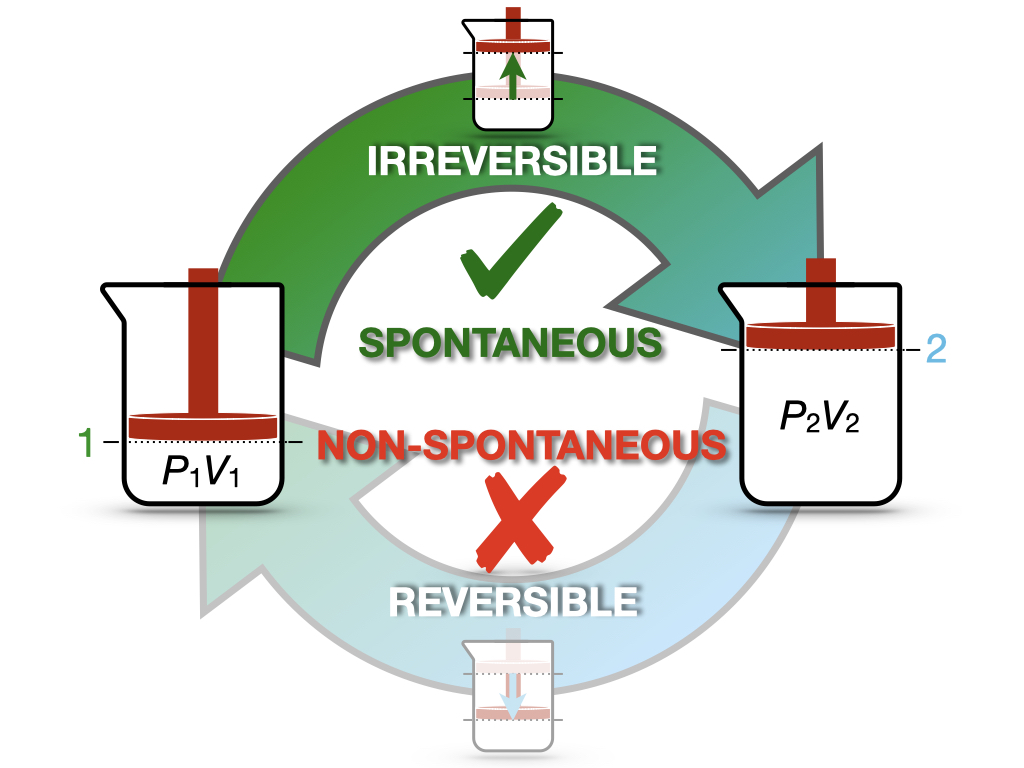
\includegraphics[width=0.8\linewidth]{./img/OEP_Figures.011} 

}

\caption{Spontaneous and Non-Spontaneous Transformations in a Cycle.}\label{fig:FigJexpC2}
\end{figure}

This cycle is similar to the cycle depicted in Figure \ref{fig:FigJexpC} for the Joule's expansion experiment. In this case, we have an intuitive understanding of the spontaneity of the irreversible expansion process, while the non-spontaneity of the backward compression. Since the cycle has at least one irreversible step, it is overall irreversible, and we can calculate:

\begin{equation}
\oint \frac{đQ_{\mathrm{IRR}}}{T} = \int_1^2 \frac{đQ_{\mathrm{IRR}}}{T} + \int_2^1 \frac{đQ_{\mathrm{REV}}}{T}.
\label{eq:qirrcycle}
\end{equation}

We can then use Clausius inequality (eq. \eqref{eq:clausiusineq}) to write:

\begin{equation}
\begin{aligned}
\int_1^2 \frac{đQ_{\mathrm{IRR}}}{T} + \int_2^1 \frac{đQ_{\mathrm{REV}}}{T} < 0,
\end{aligned}
\label{eq:qirrcycle1}
\end{equation}

which can be rearranged as:

\begin{equation}
\underbrace{\int_1^2 \frac{đQ_{\mathrm{REV}}}{T}}_{\int_1^2 dS = \Delta S} > \underbrace{\int_1^2 \frac{đQ_{\mathrm{IRR}}}{T}}_{=0},
\label{eq:qirrcycle2}
\end{equation}

where we have used the fact that, for an isolated system (the universe), \(đQ_{\mathrm{IRR}}=0\). Eq. \eqref{eq:qirrcycle2} can be rewritten as:

\begin{equation}
\Delta S > 0,
\label{eq:secondlaweq}
\end{equation}

which proves that for any irreversible process in an isolated system, the entropy is increasing. Using eq. \eqref{eq:secondlaweq} and considering that the only system that is truly isolated is the universe, we can write a concise statement for a new fundamental law of thermodynamics:

\begin{quote}
\begin{definition}
\protect\hypertarget{def:secondlawdef}{}{\label{def:secondlawdef} }\emph{Second Law of Thermodynamics:} for any spontaneous process, the entropy of the universe is increasing.
\end{definition}
\end{quote}

\renewcommand*{\standardstate}{{-\kern-6pt{\ominus}\kern-6pt-}}

\hypertarget{thirdlaw}{%
\chapter{Third Law of Thermodynamics}\label{thirdlaw}}

The Second Law can be used to infer the spontaneity of a process, as long as the entropy of the universe is considered. To do so, we need to remind ourselves that the universe can be divided into a system and its surroundings (environment). When we calculate the entropy of the universe as an indicator of the spontaneity of a process, we need to \emph{always} consider changes in entropy in \emph{both} the system (sys) and its surroundings (surr):

\begin{equation}
\Delta S^{\mathrm{universe}} = \Delta S^{\mathrm{sys}} + \Delta S^{\mathrm{surr}},
\label{eq:dsuniv}
\end{equation}

or, in differential form:

\begin{equation}
d S^{\mathrm{universe}} = d S^{\mathrm{sys}} + d S^{\mathrm{surr}},
\label{eq:dsunivd}
\end{equation}

\hypertarget{dssys}{%
\section{\texorpdfstring{Calculation of \(\Delta S^{\mathrm{sys}}\)}{Calculation of \textbackslash Delta S\^{}\{\textbackslash mathrm\{sys\}\}}}\label{dssys}}

In general \(\Delta S^{\mathrm{sys}}\) can be calculated using either its Definition \ref{def:entropy}, or its differential formula, eq. \eqref{eq:dentropy}. In practice, it is always convenient to keep in mind that entropy is a state function, and as such it does not depend on the path. For this reason, we can break every transformation into elementary steps, and calculate the entropy on any path that goes from the initial state to the final state, such as, for example:

\begin{equation}
\begin{aligned}
P_i, T_i & \quad \xrightarrow{ \Delta_{\text{TOT}} S_{\text{sys}} } \quad P_f, T_f \\
  \scriptstyle{\Delta_1 S^{\text{sys}}} & \searrow \qquad  \qquad \nearrow \; \scriptstyle{\Delta_2 S^{\text{sys}}} \\
& \qquad P_i, T_f \\
\\
\Delta_{\text{TOT}} S^{\text{sys}} & = \Delta_1 S^{\text{sys}} + \Delta_2 S^{\text{sys}},
\end{aligned}
\label{eq:entropycycle}
\end{equation}

with \(\Delta_1 S^{\text{sys}}\) calculated at constant \(P\), and \(\Delta_2 S^{\text{sys}}\) at constant \(T\). The most important elementary steps from which we can calculate the entropy resemble the prototypical processes for which we calculated the energy in section \ref{energyint}.

\hypertarget{entropy-in-isothermal-processes}{%
\subsection{Entropy in isothermal processes}\label{entropy-in-isothermal-processes}}

\begin{itemize}
\item
  For an ideal gas at constant temperature \(\Delta U =0\), and \(Q_{\mathrm{REV}} = -W_{\mathrm{REV}}\). Using the formula for \(W_{\mathrm{REV}}\) in either eq. \eqref{eq:WintsolvedV} or eq. \eqref{eq:WintsolvedP}, we obtain:
  \begin{equation}
  \Delta S^{\mathrm{sys}} = \int_i^f \frac{đQ_{\mathrm{REV}}}{T} = \frac{-W_{\mathrm{REV}}}{T} = \frac{nRT \ln \frac{V_f}{V_i}}{T} = nR \ln \frac{V_f}{V_i},
  \label{eq:sigconsttV}
  \end{equation}
  or, similarly:
  \begin{equation}
  \Delta S^{\mathrm{sys}} = nR \ln \frac{P_i}{P_f}.
  \label{eq:sigconsttP}
  \end{equation}
\item
  A phase change is a particular case of an isothermal process that does not follow the formulas introduced above since an ideal gas never liquefies. The entropy associated with a phase change at constant pressure can be calculated from its definition, remembering that \(Q_{\mathrm{rev}}= \Delta H\). For example for vaporizations:
\end{itemize}

\begin{equation}
\Delta_{\mathrm{vap}} S = \frac{\Delta_{\mathrm{vap}}H}{T_B},
\label{eq:spc}
\end{equation}

with \(\Delta_{\mathrm{vap}}H\) being the enthalpy of vaporization of a substance, and \(T_B\) its boiling temperature.

It is experimentally observed that the entropies of vaporization of many liquids have almost the same value of:

\begin{equation}
\Delta_{\mathrm{vap}} S \approx 10.5 R,
\label{eq:trouton}
\end{equation}

which corresponds in SI to the range of about 85--88 J/(mol K). This simple rule is named \textbf{Trouton's rule}, after the French scientist that discovered it, Frederick Thomas Trouton (1863-1922).

\begin{quote}
\begin{exercise}
\protect\hypertarget{exr:troutonex}{}{\label{exr:troutonex} }Calculate the standard entropy of vaporization of water knowing \(\Delta_{\mathrm{vap}} H_{\mathrm{H}_2\mathrm{O}}^{-\kern-6pt{\ominus}\kern-6pt-}= 44 \  \text{kJ/mol}\), as calculated in Exercise \ref{exr:HessLawEx}.

\emph{Solution:} Using eq. \eqref{eq:trouton}---and knowing that at standard conditions of \(P^{-\kern-6pt{\ominus}\kern-6pt-}= 1 \  \text{bar}\) the boiling temperature of water is 373 K---we calculate:

\begin{equation}
\Delta_{\mathrm{vap}} S_{\mathrm{H}_2\mathrm{O}}^{-\kern-6pt{\ominus}\kern-6pt-}= \frac{44 \times 10^3 \text{J/mol}}{373 \ \text{K}} = 118 \  \text{J/(mol K)}.
\label{eq:trouton1}
\end{equation}

The entropy of vaporization of water is far from Trouton's rule range of 85--88 J/(mol K) because of the hydrogen bond interactions between its molecules. Other similar exceptions are ethanol, formic acid, and hydrogen fluoride.
\end{exercise}
\end{quote}

\hypertarget{entropy-in-adiabatic-processes}{%
\subsection{Entropy in adiabatic processes}\label{entropy-in-adiabatic-processes}}

Since adiabatic processes happen without the exchange of heat, \(đQ=0\), it would be tempting to think that \(\Delta S^{\mathrm{sys}} = 0\) for every one of them. A transformation at constant entropy (isentropic) is always, in fact, a reversible adiabatic process. However, the opposite case is not always true, and an irreversible adiabatic transformation is usually associated with a change in entropy. To explain this fact, we need to recall that the definition of entropy includes the heat exchanged at reversible conditions only. Therefore, for irreversible adiabatic processes \(\Delta S^{\mathrm{sys}} \neq 0\). The calculation of the entropy change for an irreversible adiabatic transformation requires a substantial effort, and we will not cover it at this stage. The situation for adiabatic processes can be summarized as follows:

\begin{equation}
\begin{aligned}
\text{reversible:} \qquad & \frac{đQ_{\mathrm{REV}}}{T} = 0 \longrightarrow \Delta S^{\mathrm{sys}} = 0 \quad \text{(isentropic),}\\
\text{irreversible:} \qquad & \frac{đQ_{\mathrm{IRR}}}{T}  = 0 \longrightarrow \Delta S^{\mathrm{sys}} \neq 0. \\
\end{aligned}
\label{eq:adiabaticent}
\end{equation}

\hypertarget{entropy-in-isochoric-processes}{%
\subsection{Entropy in isochoric processes}\label{entropy-in-isochoric-processes}}

We can calculate the heat exchanged in a process that happens at constant volume, \(Q_V\), using eq. \eqref{eq:Cvint1}. Since the heat exchanged at those conditions equals the energy (eq. \eqref{eq:dUqv}), and the energy is a state function, we can use \(Q_V\) regardless of the path (reversible or irreversible). The entropy associated with the process will then be:

\begin{equation}
\Delta S^{\mathrm{sys}} = \int_i^f \frac{đQ_{\mathrm{REV}}}{T} = \int_i^f nC_V \frac{dT}{T},
\label{eq:sconstV1}
\end{equation}

which, assuming \(C_V\) independent of temperature and solving the integral on the right-hand side, becomes:

\begin{equation}
\Delta S^{\mathrm{sys}} \approx n C_V \ln \frac{T_f}{T_i}.
\label{eq:sconstV}
\end{equation}

\hypertarget{entropy-in-isobaric-processes}{%
\subsection{Entropy in isobaric processes}\label{entropy-in-isobaric-processes}}

Similarly to the constant volume case, we can calculate the heat exchanged in a process that happens at constant pressure, \(Q_P\), using eq. \eqref{eq:Cpdef}. Again, similarly to the previous case, \(Q_P\) equals a state function (the enthalpy), and we can use it regardless of the path to calculate the entropy as:

\begin{equation}
\Delta S^{\mathrm{sys}} = \int_i^f \frac{đQ_{\mathrm{REV}}}{T} = \int_i^f nC_P \frac{dT}{T},
\label{eq:sconstP1}
\end{equation}

which, assuming \(C_P\) independent of temperature and solving the integral on the right-hand side, becomes:

\begin{equation}
\Delta S^{\mathrm{sys}} \approx n C_P \ln \frac{T_f}{T_i}.
\label{eq:sconstP}
\end{equation}

\hypertarget{dssurr}{%
\section{\texorpdfstring{Calculation of \(\Delta S^{\mathrm{surr}}\)}{Calculation of \textbackslash Delta S\^{}\{\textbackslash mathrm\{surr\}\}}}\label{dssurr}}

While the entropy of the system can be broken down into simple cases and calculated using the formulas introduced above, the entropy of the surroundings does not require such a complicated treatment, and it can always be calculated as:

\begin{equation}
\Delta S^{\mathrm{surr}} = \frac{Q_{\text{surr}}}{T_{\text{surr}}}=\frac{-Q_{\text{sys}}}{T_{\text{surr}}},
\label{eq:dssurr}
\end{equation}

or, in differential form:

\begin{equation}
d S^{\mathrm{surr}} = \frac{đQ_{\text{surr}}}{T_{\text{surr}}}=\frac{-đQ_{\text{sys}}}{T_{\text{surr}}},
\label{eq:dssurrd}
\end{equation}

where the substitution \(Q_{\text{surr}}=-Q_{\text{sys}}\) can be performed regardless of whether the transformation is reversible or not. In other words, the surroundings always absorb heat reversibly. To justify this statement, we need to restrict the analysis of the interaction between the system and the surroundings to just the vicinity of the system itself. Outside of a generally restricted region, the rest of the universe is so vast that it remains untouched by anything happening inside the system.\footnote{Even if we think at the most energetic event that we could imagine happening here on earth---such as the explosion of an atomic bomb or the hit of a meteorite from outer space---such an event will not modify the average temperature of the universe by the slightest degree.} To facilitate our comprehension, we might consider a system composed of a beaker on a workbench. We can then consider the room that the beaker is in as the immediate surroundings. To all effects, the beaker+room combination behaves as a system isolated from the rest of the universe. The room is obviously much larger than the beaker itself, and therefore every energy production that happens in the system will have minimal effect on the parameters of the room. For example, an exothermal chemical reaction occurring in the beaker will not affect the overall temperature of the room substantially. When we study our reaction, \(T_{\text{surr}}\) will be constant, and the transfer of heat from the reaction to the surroundings will happen at reversible conditions.

\begin{quote}
\begin{exercise}
\protect\hypertarget{exr:supercooledEx}{}{\label{exr:supercooledEx} }Calculate the changes in entropy of the universe for the process of 1 mol of supercooled water, freezing at --10°C, knowing the following data: \(\Delta_{\mathrm{fus}}H = 6 \; \text{kJ/mol}\), \(C_P^{\mathrm{H}_2 \mathrm{O}_{(l)}}=76 \; \text{J/(mol K)}\), \(C_P^{\mathrm{H}_2 \mathrm{O}_{(s)}}=38 \; \text{J/(mol K)}\), and assuming both \(C_P\) to be independent on temperature.

\emph{Solution:} \(\Delta S^{\mathrm{sys}}\) for the process under consideration can be calculated using the following cycle:

\begin{equation}
\begin{aligned}
\mathrm{H}_2 \mathrm{O}_{(l)} & \quad \xrightarrow{\quad \Delta S_{\text{sys}} \quad} \quad \mathrm{H}_2 \mathrm{O}_{(s)} \qquad \quad T=263\;K\\
\scriptstyle{\Delta S_1} \; \bigg\downarrow \quad & \qquad \qquad \qquad \qquad \scriptstyle{\bigg\uparrow  \; \Delta S_3} \\
\mathrm{H}_2 \mathrm{O}_{(l)} & \quad \xrightarrow{\quad \Delta S_2 \qquad} \quad \mathrm{H}_2\mathrm{O}_{(s)} \qquad \; T=273\;K\\
\\
\Delta S^{\text{sys}} & = \Delta S_1 + \Delta S_2 + \Delta S_3
\end{aligned}
\label{eq:supercooledsyst}
\end{equation}

\(\Delta S_1\) and \(\Delta S_3\) are the isochoric heating and cooling processes of liquid and solid water, respectively, and can be calculated filling the given data into eq. \eqref{eq:sconstP1}. \(\Delta S_2\) is a phase change (isothermal process) and can be calculated translating eq. \eqref{eq:spc} to the freezing transformation. Overall:

\begin{equation}
\begin{aligned}
\Delta S^{\text{sys}} & = \int_{263}^{273} \frac{C_P^{\mathrm{H}_2 \mathrm{O}_{(l)}}}{T}dT+\frac{-\Delta_{\mathrm{fus}}H}{273}+\int_{273}^{263} \frac{C_P^{\mathrm{H}_2 \mathrm{O}_{(s)}}}{T}dT \\
& = 76 \ln \frac{273}{263} - \frac{6 \times 10^3}{273} + 38 \ln \frac{263}{273}= -20.6 \; \text{J/K}.
\end{aligned}
\label{eq:supercooledsyst2}
\end{equation}

Don't be confused by the fact that \(\Delta S^{\text{sys}}\) is negative. This is \textbf{\emph{not}} the entropy of the universe! Hence it tells \textbf{\emph{nothing}} about spontaneity! We can now calculate \(\Delta S^{\text{surr}}\) from \(Q_{\text{sys}}\), noting that we can calculate the enthalpy around the same cycle in eq. \eqref{eq:supercooledsyst}. To do that, we already have \(\Delta_{\mathrm{fus}}H\) from the given data, and we can calculate \(\Delta H_1\) and \(\Delta H_3\) using eq. \eqref{eq:Cpdef}.

\begin{equation}
\begin{aligned}
Q^{\text{sys}} & = \Delta H = \int_{263}^{273} C_P^{\mathrm{H}_2 \mathrm{O}_{(l)}} dT + (-\Delta_{\mathrm{fus}}H) + \int_{273}^{263} C_P^{\mathrm{H}_2 \mathrm{O}_{(s)}}dT \\
& = 76 \times 10^{-3} (273-263) - 6 + 38  \times 10^{-3} (263-273) \\ &= -5.6 \; \text{kJ}. \\
\\
\Delta S^{\text{surr}} & = \frac{-Q_{\text{sys}}}{T}=\frac{5.6 \times 10^3}{263} = + 21.3 \; \text{J/K}. \\
\end{aligned}
\label{eq:supercooledsurr}
\end{equation}

Bringing \eqref{eq:supercooledsyst} and \eqref{eq:supercooledsurr} results together, we obtain:

\begin{equation}
\Delta S^{\text{universe}}=\Delta S^{\text{sys}} + \Delta S^{\text{surr}} =  -20.6+21.3=+0.7 \; \text{J/K}.
\label{eq:supercooledfinal}
\end{equation}

Since the entropy changes in the universe are positive, the process is spontaneous, as expected.
\end{exercise}
\end{quote}

\hypertarget{spontS}{%
\section{Clausius Theorem}\label{spontS}}

By replacing eq. \eqref{eq:dssurrd} into \eqref{eq:dsunivd} we can write the differential change in the entropy of the system as:

\begin{equation}
d S^{\mathrm{sys}} = d S^{\mathrm{universe}} - d S^{\mathrm{surr}} = d S^{\mathrm{universe}} + \frac{đQ_{\text{sys}}}{T}.
\label{eq:dssysd}
\end{equation}

According to the second law, for any spontaneous process \(d S^{\mathrm{universe}}\geq0\), and therefore, replacing it into eq. \eqref{eq:dssysd}:

\begin{equation}
d S^{\mathrm{sys}} \geq \frac{đQ}{T},
\label{eq:dssyscrit7}
\end{equation}

which is the mathematical expression of the so-called \textbf{Clausius theorem}. Eq. \eqref{eq:dssyscrit7} distinguishes between three conditions:

\begin{equation}
\begin{aligned}
d S^{\mathrm{sys}} > \frac{đQ}{T} \qquad &\text{spontaneous, irreversible transformation} \\
d S^{\mathrm{sys}} = \frac{đQ}{T} \qquad &\text{reversible transformation} \\
d S^{\mathrm{sys}} < \frac{đQ}{T} \qquad &\text{non-spontaneous, irreversible transformation}, 
\end{aligned}
\label{eq:dssyscond}
\end{equation}

Clausius theorem provides a useful criterion to infer the spontaneity of a process, especially in cases where it's hard to calculate \(\Delta S^{\mathrm{universe}}\). Eq. \eqref{eq:dssyscrit7} requires knowledge of quantities that are dependent on the system exclusively, such as the difference in entropy, the amount of heat that crosses the boundaries, and the temperature at which the process happens.\footnote{In cases where the temperature of the system changes throughout the process, \(T\) is just the (constant) temperature of its immediate surroundings, \(T_{\text{surr}}\), as explained in section \ref{dssurr}.} If a process produces more entropy than the amount of heat that crosses the boundaries divided by the absolute temperature, it will be spontaneous. Vice versa, if the entropy produced is smaller than the amount of heat crossing the boundaries divided by the absolute temperature, the process will be non-spontaneous. The equality holds for systems in equilibrium with their surroundings, or for reversible processes since they happen through a series of equilibrium states. Measuring or calculating these quantities might not always be the simplest of calculations. We will return to the Clausius theorem in the next chapter when we seek more convenient indicators of spontaneity.

\hypertarget{thirdlawsect}{%
\section{The Third Law of Thermodynamics}\label{thirdlawsect}}

In chapter \ref{Thermochemistry}, we have discussed how to calculate reaction enthalpies for any reaction, given the formation enthalpies of reactants and products. In this section, we will try to do the same for reaction entropies. In this case, however, our task is simplified by a fundamental law of thermodynamics, introduced by Walther Hermann Nernst (1864--1941) in 1906.\footnote{Walther Nernst was awarded the 1920 Nobel Prize in Chemistry for his work in thermochemistry.} The statement that was initially known as Nernst's Theorem is now officially recognized as the third fundamental law of thermodynamics, and it has the following definition:

\begin{quote}
\begin{definition}
\protect\hypertarget{def:thirdlawdef}{}{\label{def:thirdlawdef} }\emph{Third Law of Thermodynamics:} The entropy of a perfectly ordered, pure, crystalline substance is zero at \(T=0 \; \text{K}\).
\end{definition}
\end{quote}

This law sets an unambiguous zero of the entropy scale, similar to what happens with absolute zero in the temperature scale. The absolute value of the entropy of every substance can then be calculated in reference to this unambiguous zero. As such, absolute entropies are always positive. This is in stark contrast to what happened for the enthalpy. An unambiguous zero of the enthalpy scale is lacking, and standard formation enthalpies (which might be negative) must be agreed upon to calculate relative differences.

In simpler terms, given a substance \(i\), we are not able to measure absolute values of its enthalpy \(H_i\) (and we must resort to known enthalpy differences, such as \(\Delta_{\mathrm{f}} H^{-\kern-6pt{\ominus}\kern-6pt-}\) at standard pressure). At the same time, for entropy, we can measure \(S_i\) thanks to the third law, and we usually report them as \(S_i^{-\kern-6pt{\ominus}\kern-6pt-}\). A comprehensive list of standard entropies of inorganic and organic compounds is reported in appendix \ref{appendix}. Reaction entropies can be calculated from the tabulated standard entropies as differences between products and reactants, using:

\begin{equation}
\Delta_{\text{rxn}} S^{-\kern-6pt{\ominus}\kern-6pt-}= \sum_i \nu_i S_i^{-\kern-6pt{\ominus}\kern-6pt-},
\label{eq:thirdlaweq}
\end{equation}

with \(\nu_i\) being the usual stoichiometric coefficients with their signs given in Definition \ref{def:nui}.

The careful wording in the definition of the third law \ref{def:thirdlawdef} allows for the fact that some crystal might form with defects (i.e., not as a perfectly ordered crystal). In this case, a residual entropy will be present even at \(T=0 \; \text{K}\). However, this residual entropy can be removed, at least in theory, by forcing the substance into a perfectly ordered crystal.\footnote{A procedure that---in practice---might be extremely difficult to achieve.}

An interesting corollary to the third law states that it is impossible to find a procedure that reduces the temperature of a substance to \(T=0 \; \text{K}\) in a finite number of steps.

\hypertarget{Potentials}{%
\chapter{Thermodynamic Potentials}\label{Potentials}}

\hypertarget{fundeq}{%
\section{Fundamental Equation of Thermodynamics}\label{fundeq}}

Let's summarize some of the results from the first and second law of thermodynamics that we have seen so far. For reversible processes in closed systems:

\begin{equation}
\begin{aligned}
\text{From 1}^{\text{st}} \text{ Law:} \qquad \quad & dU = đQ_{\mathrm{REV}}-PdV \\
\text{From The Definition of Entropy:} \qquad \quad & dS = \frac{đQ_{\mathrm{REV}}}{T} \rightarrow đQ_{\mathrm{REV}} = TdS \\
\\
\Rightarrow \quad & dU = TdS - PdV.
\end{aligned}
\label{eq:dunv}
\end{equation}

Eq. \eqref{eq:dunv} is called the \textbf{fundamental equation of thermodynamics} since it combines the first and the second laws. Even though we started the derivation above by restricting to reversible transformations only, if we look carefully at eq. \eqref{eq:dunv}, we notice that it exclusively involves state functions. As such, it applies to both reversible and irreversible processes. The fundamental equation, however, remains constrained to closed systems. This fact restricts its utility for chemistry, since when a chemical reaction happens, the mass in the system will change, and the system is no longer closed.

At the end of the 19\textsuperscript{th} century, Josiah Willard Gibbs (1839--1903) proposed an important addition to the fundamental equation to account for chemical reactions. Gibbs was able to do so by introducing a new quantity that he called the chemical potential:

\begin{quote}
\begin{definition}
\protect\hypertarget{def:chemicalpot}{}{\label{def:chemicalpot} }The \emph{chemical potential} is the amount of energy absorbed or released due to a change of the particle number of a given chemical species.
\end{definition}
\end{quote}

The chemical potential of species \(i\) is usually abbreviated as \(\mu_i\), and it enters the fundamental equation of thermodynamics as:

\begin{equation}
dU = TdS-PdV+\sum_i\mu_i dn_i,
\label{eq:dunv2}
\end{equation}

where \(dn_i\) is the differential change in the number of moles of substance \(i\), and the summation extends over all chemical species in the system.

According to the fundamental equation, the internal energy of a system is a function of the three variables entropy, \(S\), volume, \(V\), and the numbers of moles \(\{n_i\}\).\footnote{In the case of the numbers of moles we include them in curly brackets to indicate that there might be more than one, depending on how many species undergo chemical reactions.} Because of their importance in determining the internal energy, these three variables are crucial in thermodynamics. Under several circumstances, however, they might not be the most convenient variables to use.\footnote{For example, we don't always have a simple way to calculate or to measure the entropy.} To emphasize the important connections given by the fundamental equation, we can use the notation \(U(S,V,\{n_i\})\) and we can term \(S\), \(V\), and \(\{n_i\}\) \textbf{natural variables} of the energy.

\hypertarget{thermpot}{%
\section{Thermodynamic Potentials}\label{thermpot}}

Starting from the fundamental equation, we can define new thermodynamic state functions that are more convenient to use under certain specific conditions. The new functions are determined by using a mathematical procedure called the Legendre transformation. A Legendre transformation is a linear change in variables that brings from an initial mathematical function to a new function obtained by subtracting one or more products of conjugate variables.\footnote{The mathematical condition that is fulfilled when performing a Legendre transformation is that the first derivatives of the original function and its transformation are inverse functions of each other.}

Taking the internal energy as defined in eq. \eqref{eq:dunv}, we can perform such procedure by subtracting products of the following conjugate variables pairs: \(T \text{ and } S\) or \(-P \text{ and } V\). This procedure aims to define new state functions that depend on more convenient natural variables.\footnote{The rigorous mathematical definition of conjugate variables is unimportant at this stage. However, we can relate the variables in a pair with basic physics by noticing how the first variable in a pair is always intensive (\(T\) and \(-P\)), while the second one is always extensive (\(S\) and \(V\)). The intensive variables represent thermodynamic drivinng forces (as compared with mechanical forces in classical mechanics), while the extensive ones are the thermodynamic displacements (as compared with spatial displacements in classical mechanics). Similarly to classical mechanics, the product of two conjugate variables in a pair yields an energy. The minus sign in front of \(P\) is explained by the fact that an increase in the force should always correspond to an increase in the displacement (while \(P\) and \(V\) are inversely related).} The new functions are called ``thermodynamic potential energies,'' or simply \textbf{thermodynamic potentials}.\footnote{Even if we introduced both concepts in the same chapter, it is important to never confuse the \emph{thermodynamic potentials}---which are potential energy functions---with the \emph{chemical potential}---which have been introduced by Gibbs to study heat in chemical reactions.} An example of this procedure is given by the definition of enthalpy that we have already seen in section \ref{enthalpy}. If we take the internal energy and subtract the product of two conjugate variables (\(-P\) and \(V\)), we obtain a new state function called enthalpy, as we did in eq. \eqref{eq:enthalpydef}). Taking the differential of this definition, we obtain:

\begin{equation}
dH = dU +VdP +PdV,
\label{eq:dhdef1}
\end{equation}

and using the fundamental equation, eq. \eqref{eq:dunv2}, to replace \(dU\), we obtain:

\begin{equation}
\begin{aligned}
dH & = TdS -PdV +\sum_i\mu_i dn_i +VdP +PdV  \\
   & = TdS +VdP +\sum_i\mu_i dn_i.
\end{aligned}
\label{eq:dhdef2}
\end{equation}

which is the fundamental equation for enthalpy. The natural variables of the enthalpy are \(S\), \(P\), and \(\{n_i\}\). The Legendre transformation has allowed us to go from \(U(S,V,\{n_i\})\) to \(H(S,P,\{n_i\})\) by replacing the dependence on the extensive variable, \(V\), with an intensive one, \(P\).

Following the same procedure, we can perform another Legendre transformation to replace the entropy with a more convenient intensive variable such as the temperature. This can be done by defining a new function called the Helmholtz free energy, \(A\), as:

\begin{equation}
A = U -TS
\label{eq:dadef1}
\end{equation}

which, taking the differential and using the fundamental equation (eq. \eqref{eq:dunv2}) becomes:

\begin{equation}
\begin{aligned}
dA &= dU -SdT -TdS = TdS - PdV +\sum_i \mu_i dn_i -SdT -TdS  \\
   &= -SdT -PdV +\sum_i \mu_i dn_i.
\end{aligned}
\label{eq:dadef2}
\end{equation}

The Helmholtz free energy is named after Hermann Ludwig Ferdinand von Helmholtz (1821---1894), and its natural variables are temperature, volume, and the number of moles.

Finally, suppose we perform a Legendre transformation on the internal energy to replace both the entropy and the volume with intensive variables. In that case, we can define a new function called the Gibbs free energy, \(G\), as:

\begin{equation}
G = U -TS +PV
\label{eq:dgdef1}
\end{equation}

which, taking again the differential and using eq. \eqref{eq:dunv2} becomes:

\begin{equation}
\begin{aligned}
dG &= dU -SdT -TdS +VdP +PdV \\
   &= TdS - PdV +\sum_i\mu_i dn_i -SdT -TdS +VdP +PdV \\
   &= VdP -SdT +\sum_i\mu_i dn_i.
\end{aligned}
\label{eq:dgdef2}
\end{equation}

The Gibbs free energy is named after Willard Gibbs himself, and its natural variables are temperature, pressure, and number of moles.

A summary of the four thermodynamic potentials is given in the following table.

\tiny

\begin{longtable}[]{@{}cccc@{}}
\toprule
\textbf{Name} & \textbf{Symbol} & \textbf{Fundamental Equation} & \textbf{Natural Variables}\tabularnewline
\midrule
\endhead
\textbf{Energy} & \(U\) & \(dU=TdS-PdV+\sum_i\mu_i dn_i\) & \(S,V,\{n_i\}\)\tabularnewline
\textbf{Enthalpy} & \(H\) & \(dH=TdS+VdP+\sum_i\mu_i dn_i\) & \(S,P,\{n_i\}\)\tabularnewline
\textbf{Helmholtz Free Energy} & \(A\) & \(dA=-SdT-PdV+\sum_i\mu_i dn_i\) & \(T,V,\{n_i\}\)\tabularnewline
\textbf{Gibbs Free Energy} & \(G\) & \(dG=VdP-SdT+\sum_i\mu_i dn_i\) & \(T,P,\{n_i\}\)\tabularnewline
\bottomrule
\end{longtable}

\normalsize

The thermodynamic potentials are the analog of the potential energy in classical mechanics. Since the potential energy is interpreted as the capacity to do work, the thermodynamic potentials assume the following interpretations:

\begin{itemize}
\tightlist
\item
  Internal energy (\(U\)) is the capacity to do work plus the capacity to release heat.
\item
  Enthalpy (\(H\)) is the capacity to do non-mechanical work plus the capacity to release heat.
\item
  Gibbs free energy (\(G\)) is the capacity to do non-mechanical work.
\item
  Helmholtz free energy (\(A\)) is the capacity to do mechanical plus non-mechanical work.\footnote{For the mathematically inclined, an entertaining method to summarize the same thermodynamic potentials is the \href{https://en.wikipedia.org/wiki/Thermodynamic_square}{thermodynamic square}.}
\end{itemize}

Where non-mechanical work is defined as any type of work that is not expansion or compression (\(PV\)--work). A typical example of non-mechanical work is electrical work.

\hypertarget{freeenergies}{%
\section{Free Energies}\label{freeenergies}}

The Legendre transformation procedure translates all information contained in the original function to the new one. Therefore, \(H(S,P,\{n_i\})\), \(A(T,V,\{n_i\})\), and \(G(T,P,\{n_i\})\) all contain the same information that is in \(U(S,V,\{n_i\})\). However, the new functions depend on different natural variables, and they are useful at different conditions. For example, when we want to study chemical changes, we are interested in studying the term \(\sum_i\mu_i dn_i\) that appears in each thermodynamic potential. To do so, we need to isolate the chemical term by keeping all other natural variables constant. For example, changes in the chemical term will correspond to changes in the internal energy at constant \(S\) and constant \(V\):

\begin{equation}
dU(S,V,\{n_i\}) = \sum_i\mu_i dn_i \quad \text{if} \quad dS=dV=0.
\label{eq:duchem}
\end{equation}

Similarly:

\begin{equation}
\begin{aligned}
dH(S,P,\{n_i\}) = \sum_i\mu_i dn_i \quad \text{if} \quad dS=dP=0, \\
dA(T,V,\{n_i\}) = \sum_i\mu_i dn_i \quad \text{if} \quad dT=dV=0, \\
dG(T,P,\{n_i\}) = \sum_i\mu_i dn_i \quad \text{if} \quad dT=dP=0.
\end{aligned}
\label{eq:dhagchem}
\end{equation}

The latter two cases are particularly interesting since most of chemistry happens at either constant volume,\footnote{for example, several industrial processes in chemical plants.} or constant pressure.\footnote{for example, most processes in a chemistry lab.} Since \(dS=0\) is not a requirement for both free energies to describe chemical changes, we can apply either of them to study non-isentropic processes. If a process is not isentropic, it either increases the entropy of the universe, or it decreases it. Therefore---according to the second law---it is either spontaneous or not. Using this concept in conjunction with Clausius theorem, we can devise new criteria for inferring the spontaneity of a process that depends exclusively on the free energies.

Recalling Clausius theorem:

\begin{equation}
d S^{\mathrm{sys}} \geq \frac{đQ}{T_{\text{surr}}} \quad \longrightarrow \quad TdS \geq đQ,
\label{eq:dssyscrit}
\end{equation}

we can consider the two cases: constant \(V\) (\(đQ_V=dU\), left), and constant \(P\) (\(đQ_P=dH\), right):

\begin{equation}
\begin{aligned}
\text{constant} & \; V:           & \qquad \qquad & \qquad \qquad &     \text{constant} & \; P: \\
\\
TdS & \geq dU           & &   &     TdS & \geq dH \\
\\
TdS -dU & \geq 0         & &   &      TdS -dH & \geq 0 \\
\end{aligned}
\label{eq:dadgder1}
\end{equation}

we can then simplify the definition of free energies, eqs. \eqref{eq:dadef2} and \eqref{eq:dgdef2}:

\begin{equation}
\begin{aligned}
\text{constant} & \; T,V:           & \qquad & \qquad &     \text{constant} & \; T,P: \\
\\
d(A)_{T,V} &= dU -TdS     & &   &       d(G)_{T,P} &= dH - TdS \\ 
\\
dU = d(A)_{T,V} &+TdS       & &   &       dH = d(G)_{T,P} &+TdS
\end{aligned}
\label{eq:dadgder3}
\end{equation}

and by merging \(dU\) and \(dH\) from eqs. \eqref{eq:dadgder3} into Clausius theorem expressed using eqs. \eqref{eq:dadgder1}, we obtain:

\begin{equation}
\begin{aligned}
TdS -d(A)_{T,V} &- TdS \geq 0 & \qquad & \qquad & TdS -d(G)_{T,P} &- TdS \geq 0 \\
\\
d(A)_{T,V} & \leq 0 & \qquad & \qquad & d(G)_{T,P} & \leq 0. \\
\end{aligned}
\label{eq:dadgcond}
\end{equation}

These equations represent the conditions on \(dA\) and \(dG\) for inferring the spontaneity of a process, and can be summarized as follows:

\begin{quote}
\begin{definition}
\protect\hypertarget{def:helmgibbsminimum}{}{\label{def:helmgibbsminimum} }\(\;\)

\begin{itemize}
\tightlist
\item
  During a spontaneous process at constant \emph{temperature} and \emph{volume}, the \emph{Helmholtz free energy} will decrease \((dA<0)\), until it reaches a stationary point at which the system will be at equilibrium \((dA=0)\).
\item
  During a spontaneous process at constant \emph{temperature} and \emph{pressure}, the \emph{Gibbs free energy} will decrease \((dG<0)\), until it reaches a stationary point at which the system will be at equilibrium \((dG=0)\).
\end{itemize}
\end{definition}
\end{quote}

\begin{figure}

{\centering 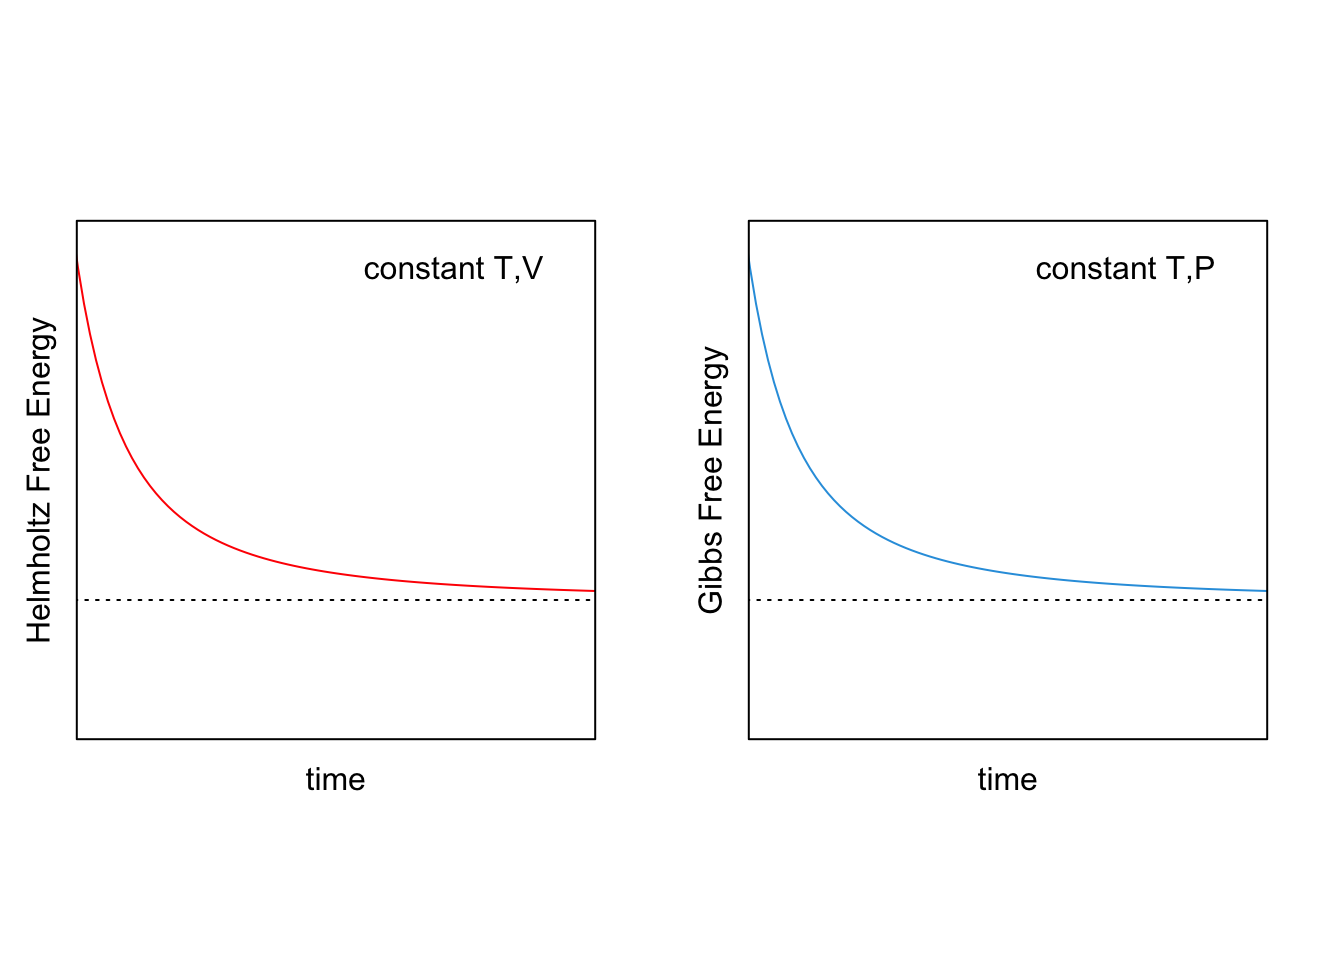
\includegraphics{pchem1_files/figure-latex/agfig-1} 

}

\caption{Behavior of Helmholtz (red) and Gibbs (blue) Free Energies for Spontaneous Processes at Constant $T,V$ (left) and Constant $T,P$ (right).}\label{fig:agfig}
\end{figure}

\hypertarget{maxwell}{%
\section{Maxwell Relations}\label{maxwell}}

Let's consider the fundamental equations for the thermodynamic potentials that we have derived in section \ref{fundeq}:

\begin{equation}
\begin{aligned}
dU(S,V,\{n_i\}) &= \enspace T dS -P dV + \sum_i \mu_i dn_i \\
dH(S,P,\{n_i\}) &= \enspace T dS + V dP + \sum_i \mu_i dn_i \\
dA(T,V,\{n_i\}) &= -S dT -P dV + \sum_i \mu_i dn_i \\
dG(T,P,\{n_i\}) &= -S dT + V dP + \sum_i \mu_i dn_i\;.
\end{aligned}
\label{eq:dhagchem1}
\end{equation}

From the knowledge of the natural variable of each potential, we could reconstruct these formulas by using the total differential formula:

\begin{equation}
\begin{aligned}
dU &= \underbrace{\left(\frac{\partial U}{\partial S} \right)_{V,\{n_i\}}}_{T} dS + \underbrace{\left(\frac{\partial U}{\partial V} \right)_{S,\{n_i\}}}_{-P} dV + \sum_i \underbrace{\left(\frac{\partial U}{\partial n_i} \right)_{S,V,\{n_{j \neq i}\}}}_{\mu_i} dn_i \\
dH &= \underbrace{\left(\frac{\partial H}{\partial S} \right)_{P,\{n_i\}}}_{T} dS + \underbrace{\left(\frac{\partial H}{\partial P} \right)_{S,\{n_i\}}}_{V} dP + \sum_i \underbrace{\left(\frac{\partial H}{\partial n_i} \right)_{S,P,\{n_{j \neq i}\}}}_{\mu_i} dn_i \\
dA &= \underbrace{\left(\frac{\partial A}{\partial T} \right)_{V,\{n_i\}}}_{-S} dT + \underbrace{\left(\frac{\partial A}{\partial V} \right)_{T,\{n_i\}}}_{-P} dV + \sum_i \underbrace{\left(\frac{\partial A}{\partial n_i} \right)_{T,V,\{n_{j \neq i}\}}}_{\mu_i} dn_i \\
dG &= \underbrace{\left(\frac{\partial G}{\partial T} \right)_{V,\{n_i\}}}_{-S} dT + \underbrace{\left(\frac{\partial G}{\partial P} \right)_{T,\{n_i\}}}_{V} dP + \sum_i \underbrace{\left(\frac{\partial G}{\partial n_i} \right)_{T,P,\{n_{j \neq i}\}}}_{\mu_i} dn_i\;,
\end{aligned}
\label{eq:dhagchem2}
\end{equation}

we can derive the following new definitions:

\begin{equation}
\begin{aligned}
 T &= \left(\frac{\partial U}{\partial S} \right)_{V,\{n_i\}} = \left(\frac{\partial H}{\partial S} \right)_{P,\{n_i\}}  \\
-P &= \left(\frac{\partial U}{\partial V} \right)_{S,\{n_i\}} = \left(\frac{\partial A}{\partial V} \right)_{T,\{n_i\}}  \\
 V &= \left(\frac{\partial H}{\partial P} \right)_{S,\{n_i\}} = \left(\frac{\partial G}{\partial P} \right)_{T,\{n_i\}}  \\
-S &= \left(\frac{\partial A}{\partial T} \right)_{V,\{n_i\}} = \left(\frac{\partial G}{\partial T} \right)_{V,\{n_i\}}  \\
\text{and:}
\\
 \mu_i &=  \left(\frac{\partial U}{\partial n_i} \right)_{S,V,\{n_{j \neq i}\}} =  \left(\frac{\partial H}{\partial n_i} \right)_{S,P,\{n_{j \neq i}\}} \\
       &= \left(\frac{\partial A}{\partial n_i} \right)_{T,V,\{n_{j \neq i}\}} = \left(\frac{\partial G}{\partial n_i} \right)_{T,P,\{n_{j \neq i}\}}\;.
\end{aligned}
\label{eq:dhagchem3}
\end{equation}

Since \(T\), \(P\), \(V\), and \(S\) are now defined as partial first derivatives of a thermodynamic potential, we can now take a second partial derivation with respect to a separate variable, and rely on Schwartz's theorem to derive the following relations:

\begin{equation}
\begin{aligned}
\frac{\partial^2 U }{\partial S \partial V} &=& +\left(\frac{\partial T}{\partial V}\right)_{S,\{n_{j \neq i}\}} &=& -\left(\frac{\partial P}{\partial S}\right)_{V,\{n_{j \neq i}\}}   \\
\frac{\partial^2 H }{\partial S \partial P} &=& +\left(\frac{\partial T}{\partial P}\right)_{S,\{n_{j \neq i}\}} &=& +\left(\frac{\partial V}{\partial S}\right)_{P,\{n_{j \neq i}\}}  \\
-\frac{\partial^2 A }{\partial T \partial V} &=& +\left(\frac{\partial S}{\partial V}\right)_{T,\{n_{j \neq i}\}} &=& +\left(\frac{\partial P}{\partial T}\right)_{V,\{n_{j \neq i}\}}  \\
\frac{\partial^2 G }{\partial T \partial P} &=& -\left(\frac{\partial S}{\partial P}\right)_{T,\{n_{j \neq i}\}} &=& +\left(\frac{\partial V}{\partial T}\right)_{P,\{n_{j \neq i}\}}
\end{aligned}
\label{eq:maxrelf}
\end{equation}

The relations in \eqref{eq:maxrelf} are called \textbf{Maxwell relations},\footnote{Maxwell relations should not be confused with the Maxwell equations of electromagnetism.} and are useful in experimental settings to relate quantities that are hard to measure with others that are more intuitive.

\begin{quote}
\begin{exercise}
\protect\hypertarget{exr:maxwellEx}{}{\label{exr:maxwellEx} }Derive the last Maxwell relation in eq. \eqref{eq:maxrelf}.

\emph{Solution:} We can start our derivation from the definition of \(V\) and \(S\) as a partial derivative of \(G\):

\begin{equation}
 V = \left(\frac{\partial G}{\partial P} \right)_{T,\{n_i\}} \qquad \text{and:} \qquad -S = \left(\frac{\partial G}{\partial T} \right)_{V,\{n_i\}},
\end{equation}

and then take a second partial derivative of each quantity with respect to the second variable:

\begin{equation}
\begin{aligned}
 \left(\frac{\partial V}{\partial T} \right)_{P,\{n_i\}} &=\frac{\partial}{\partial T}\left[ \left(\frac{\partial G}{\partial P} \right)_{T,\{n_i\}} \right]_{P,\{n_i\}} \\
\\
-\left(\frac{\partial S}{\partial P} \right)_{T,\{n_i\}} &=\frac{\partial}{\partial P}\left[ \left(\frac{\partial G}{\partial T} \right)_{P,\{n_i\}} \right]_{T,\{n_i\}} \;.
\end{aligned}
\end{equation}

These two derivatives are mixed partial second derivatives of \(G\) with respect to \(T\) and \(P\), and therefore, according to Schwartz's theorem, they are equal to each other:

\begin{equation}
\begin{aligned}
\frac{\partial}{\partial T}\left[ \left(\frac{\partial G}{\partial P} \right)_{T,\{n_i\}} \right]_{P,\{n_i\}} &=
\frac{\partial}{\partial P}\left[ \left(\frac{\partial G}{\partial T} \right)_{P,\{n_i\}} \right]_{T,\{n_i\}}, \\
\\
\text{hence:} \\
\\
 \left(\frac{\partial V}{\partial T} \right)_{P,\{n_i\}} &= -\left(\frac{\partial S}{\partial P} \right)_{T,\{n_i\}},
\end{aligned}
\end{equation}

which is the last of Maxwell relations, as defined in eq. \eqref{eq:maxrelf}. This relation is particularly useful because it connects the quantity \(\left(\frac{\partial S}{\partial P} \right)_{T,\{n_i\}}\)---which is impossible to measure in a lab---with the quantity \(\left(\frac{\partial V}{\partial T} \right)_{P,\{n_i\}}\)---which is easier to measure from an experiment that determines isobaric volumetric thermal expansion coefficients.
\end{exercise}
\end{quote}

\renewcommand*{\standardstate}{{-\kern-6pt{\ominus}\kern-6pt-}}

\hypertarget{GibbsFree}{%
\chapter{Gibbs Free Energy}\label{GibbsFree}}

In this chapter, we will concentrate on chemical processes that happen at constant \(T\) and constant \(P\).\footnote{The majority of chemical reactions in a lab happens at those conditions, and all biological functions happen at those conditions as well.} As such, we will focus our attention on the Gibbs free energy.

\hypertarget{gibbseqsec}{%
\section{Gibbs Equation}\label{gibbseqsec}}

Recalling from the previous chapter, the definition of \(G\) is:

\begin{equation}
G = U -TS +PV = H-TS,
\label{eq:dgdeftot}
\end{equation}

which, taking the differential at constant \(T\) and \(P\), becomes:

\begin{equation}
dG = dH \; \overbrace{-SdT}^{=0} -TdS = dH -TdS.
\label{eq:dgdeftot2}
\end{equation}

Integrating eq. \eqref{eq:dgdeftot2} between the initial and final states of a process results in:

\begin{equation}
\begin{aligned}
\int_i^f dG &= \int_i^f dH -T \int_i^f dS \\
\\
\Delta G &= \Delta H -T \Delta S
\end{aligned}
\label{eq:gibbseq}
\end{equation}

which is the famous \textbf{Gibbs equation} for \(\Delta G\). Using Definition \ref{def:helmgibbsminimum}, we can use \(\Delta G\) to infer the spontaneity of a chemical process that happens at constant \(T\) and \(P\) using \(\Delta G \leq 0\). If we set ourselves at standard conditions, we can calculate the standard Gibbs free energy of formation, \(\Delta_{\text{rxn}} G^{-\kern-6pt{\ominus}\kern-6pt-}\), for any reaction as:

\begin{equation}
\begin{aligned}
\Delta_{\text{rxn}} G^{-\kern-6pt{\ominus}\kern-6pt-}&= \Delta_{\text{rxn}} H^{-\kern-6pt{\ominus}\kern-6pt-}-T \Delta_{\text{rxn}} S^{-\kern-6pt{\ominus}\kern-6pt-}\\
\\
&= \sum_i \nu_i \Delta_{\mathrm{f}} H_i^{-\kern-6pt{\ominus}\kern-6pt-}+ T \sum_i \nu_i S_i^{-\kern-6pt{\ominus}\kern-6pt-},
\end{aligned}
\label{eq:gibbseq2}
\end{equation}

where \(\Delta_{\mathrm{f}} H_i^{-\kern-6pt{\ominus}\kern-6pt-}\) are the standard enthalpies of formation, \(S_i^{-\kern-6pt{\ominus}\kern-6pt-}\) are the standard entropies, and \(\nu_i\) are the stoichiometric coefficients for every species \(i\) involved in the reaction. All these quantities are commonly available, and we have already discussed their usage in chapters \ref{Thermochemistry} and \ref{thirdlaw}, respectively.\footnote{It is not uncommon to see values of \(\Delta_{\text{f}} G^{-\kern-6pt{\ominus}\kern-6pt-}\) tabulated alongside \(\Delta_{\mathrm{f}} H^{-\kern-6pt{\ominus}\kern-6pt-}\) and \(S_i^{-\kern-6pt{\ominus}\kern-6pt-}\), which simplifies even further the calculation. In fact, a comprehensive list of standard Gibbs free energy of formation of inorganic and organic compounds is reported in the appendix of this book \ref{appendix}. For cases where \(\Delta_{\text{f}} G^{-\kern-6pt{\ominus}\kern-6pt-}\) are not reported, they can always be calculated by their constituents.}

The following four options are possible for \(\Delta G^{-\kern-6pt{\ominus}\kern-6pt-}\) of a chemical reaction:

\begin{longtable}[]{@{}clccc@{}}
\toprule
\begin{minipage}[b]{(\columnwidth - 4\tabcolsep) * \real{0.17}}\centering
\(\Delta G^{-\kern-6pt{\ominus}\kern-6pt-}\)\strut
\end{minipage} & \begin{minipage}[b]{(\columnwidth - 4\tabcolsep) * \real{0.04}}\raggedright
\strut
\end{minipage} & \begin{minipage}[b]{(\columnwidth - 4\tabcolsep) * \real{0.17}}\centering
\(\Delta H^{-\kern-6pt{\ominus}\kern-6pt-}\)\strut
\end{minipage} & \begin{minipage}[b]{(\columnwidth - 4\tabcolsep) * \real{0.17}}\centering
\(\Delta S^{-\kern-6pt{\ominus}\kern-6pt-}\)\strut
\end{minipage} & \begin{minipage}[b]{(\columnwidth - 4\tabcolsep) * \real{0.45}}\centering
Spontaneous?\strut
\end{minipage}\tabularnewline
\midrule
\endhead
\begin{minipage}[t]{(\columnwidth - 4\tabcolsep) * \real{0.17}}\centering
--\strut
\end{minipage} & \begin{minipage}[t]{(\columnwidth - 4\tabcolsep) * \real{0.04}}\raggedright
\emph{if}\strut
\end{minipage} & \begin{minipage}[t]{(\columnwidth - 4\tabcolsep) * \real{0.17}}\centering
--\strut
\end{minipage} & \begin{minipage}[t]{(\columnwidth - 4\tabcolsep) * \real{0.17}}\centering
+\strut
\end{minipage} & \begin{minipage}[t]{(\columnwidth - 4\tabcolsep) * \real{0.45}}\centering
\emph{Always}\strut
\end{minipage}\tabularnewline
\begin{minipage}[t]{(\columnwidth - 4\tabcolsep) * \real{0.17}}\centering
+\strut
\end{minipage} & \begin{minipage}[t]{(\columnwidth - 4\tabcolsep) * \real{0.04}}\raggedright
\emph{if}\strut
\end{minipage} & \begin{minipage}[t]{(\columnwidth - 4\tabcolsep) * \real{0.17}}\centering
+\strut
\end{minipage} & \begin{minipage}[t]{(\columnwidth - 4\tabcolsep) * \real{0.17}}\centering
--\strut
\end{minipage} & \begin{minipage}[t]{(\columnwidth - 4\tabcolsep) * \real{0.45}}\centering
\emph{Never}\strut
\end{minipage}\tabularnewline
\begin{minipage}[t]{(\columnwidth - 4\tabcolsep) * \real{0.17}}\centering
--/+\strut
\end{minipage} & \begin{minipage}[t]{(\columnwidth - 4\tabcolsep) * \real{0.04}}\raggedright
\emph{if}\strut
\end{minipage} & \begin{minipage}[t]{(\columnwidth - 4\tabcolsep) * \real{0.17}}\centering
--\strut
\end{minipage} & \begin{minipage}[t]{(\columnwidth - 4\tabcolsep) * \real{0.17}}\centering
--\strut
\end{minipage} & \begin{minipage}[t]{(\columnwidth - 4\tabcolsep) * \real{0.45}}\centering
\emph{Depends on \(T\):} \(\scriptstyle{\text{spontaneous at low } T}\)\strut
\end{minipage}\tabularnewline
\begin{minipage}[t]{(\columnwidth - 4\tabcolsep) * \real{0.17}}\centering
+/--\strut
\end{minipage} & \begin{minipage}[t]{(\columnwidth - 4\tabcolsep) * \real{0.04}}\raggedright
\emph{if}\strut
\end{minipage} & \begin{minipage}[t]{(\columnwidth - 4\tabcolsep) * \real{0.17}}\centering
+\strut
\end{minipage} & \begin{minipage}[t]{(\columnwidth - 4\tabcolsep) * \real{0.17}}\centering
+\strut
\end{minipage} & \begin{minipage}[t]{(\columnwidth - 4\tabcolsep) * \real{0.45}}\centering
\emph{Depends on \(T\):} \(\scriptstyle{\text{spontaneous at high } T}\)\strut
\end{minipage}\tabularnewline
\bottomrule
\end{longtable}

Or, in other words:

\begin{itemize}
\tightlist
\item
  Exothermic reactions that increase the entropy are always spontaneous.
\item
  Endothermic reactions that reduce the entropy are always non-spontaneous.
\item
  For the other two cases, the spontaneity of the reaction depends on the temperature:

  \begin{itemize}
  \tightlist
  \item
    Exothermic reactions that reduce the entropy are spontaneous at low \(T\).
  \item
    Endothermic reactions that increase the entropy are spontaneous at high \(T\).
  \end{itemize}
\end{itemize}

A simple criterion to evaluate the entropic contribution of a reaction is to look at the total number of moles of the reactants and the products (as the sum of the stoichiometric coefficients). If the reaction is producing more molecules than it destroys \(\left( \left| \sum_\text{products} \nu_i \right| > \left| \sum_\text{reactants} \nu_i \right| \right)\), it will increase the entropy. Vice versa, if the total number of moles in a reaction is reducing \(\left( \left| \sum_\text{products} \nu_i \right| < \left| \sum_\text{reactants} \nu_i \right| \right)\), the entropy will also reduce.

As we saw in section \ref{thermpot}, the natural variables of the Gibbs free energy are the temperature, \(T\), the pressure, \(P\), and chemical composition, as the number of moles \(\{n_i\}\). The Gibbs free energy can therefore be expressed using the total differential as (see also, last formula in eq. \eqref{eq:dhagchem2}):

\begin{equation}
dG(T,P,\{n_i\}) = \mkern-18mu \underbrace{\left(\frac{\partial G}{\partial T} \right)_{V,\{n_i\}}}_{\text{temperature dependence}} \mkern-36mu dT + \underbrace{\left(\frac{\partial G}{\partial P} \right)_{T,\{n_i\}}}_{\text{pressure dependence}} \mkern-36mu dP + \sum_i \underbrace{\left(\frac{\partial G}{\partial n_i} \right)_{T,P,\{n_{j \neq i}\}}}_{\text{composition dependence}} \mkern-36mu dn_i.
\label{eq:dgtotdiff}
\end{equation}

If we know the behavior of \(G\) as we vary each of the three natural variables independently of the other two, we can reconstruct the total differential \(dG\). Each of these terms represents a coefficient in eq. \eqref{eq:dgtotdiff}, which are given in eq. \eqref{eq:dhagchem3}.

\hypertarget{temperature-dependence-of-delta-g}{%
\section{\texorpdfstring{Temperature Dependence of \(\Delta G\)}{Temperature Dependence of \textbackslash Delta G}}\label{temperature-dependence-of-delta-g}}

\[
\left(\frac{\partial G}{\partial T} \right)_{P,\{n_i\}}=-S
\]

Let's analyze the first coefficient that gives the dependence of the Gibbs energy on temperature. Since this coefficient is equal to \(-S\) and the entropy is always positive, \(G\) must decrease when \(T\) increases at constant \(P\) and \(\{n_i\}\), and vice versa.

If we replace this coefficient for \(-S\) in the Gibbs equation, eq. \eqref{eq:gibbseq}, we obtain:

\begin{equation}
\Delta G = \Delta H + T \left(\frac{\partial \Delta G}{\partial T} \right)_{P,\{n_i\}},
\label{eq:dgconsttt}
\end{equation}

and since eq. \eqref{eq:dgconsttt} includes both \(\Delta G\) and its partial derivative with respect to temperature \(\left(\frac{\partial \Delta G}{\partial T} \right)_{P,\{n_i\}}\) we need to rearrange it to include the temperature derivative only. To do so, we can start by evaluating the partial derivative of \(\left( \frac{\Delta G}{T} \right)\) using the chain rule:

\begin{equation}
\left[ \frac{\partial\left( \frac{\Delta G}{T} \right)}{\partial T} \right]_{P,\{n_i\}} = \frac{1}{T} \left(\frac{\partial \Delta G}{\partial T}  \right)_{P,\{n_i\}} - \frac{1}{T^2}\Delta G,
\label{eq:dgconsttt1}
\end{equation}

which, replacing \(\Delta G\) from eq. \eqref{eq:dgconsttt} into eq. \eqref{eq:dgconsttt1}, becomes:

\begin{equation}
\begin{aligned}
\left[ \frac{\partial\left( \frac{\Delta G}{T} \right)}{\partial T} \right]_{P,\{n_i\}} &= \frac{1}{T} \left(\frac{\partial \Delta G}{\partial T}  \right)_{P,\{n_i\}} - \frac{1}{T^2} \left[ \Delta H + T \left(\frac{\partial \Delta G}{\partial T} \right)_{P,\{n_i\}} \right] \\
&= \frac{1}{T} \left(\frac{\partial \Delta G}{\partial T}  \right)_{P,\{n_i\}}- \frac{\Delta H}{T^2}-\frac{1}{T} \left(\frac{\partial \Delta G}{\partial T}  \right)_{P,\{n_i\}},
\end{aligned}
\label{eq:dgconsttt2}
\end{equation}

which simplifies to:

\begin{equation}
\begin{aligned}
\left[ \frac{\partial\left( \frac{\Delta G}{T} \right)}{\partial T} \right]_{P,\{n_i\}} &= - \frac{\Delta H}{T^2}.
\end{aligned}
\label{eq:gibbshelm}
\end{equation}

Equation \eqref{eq:gibbshelm} is known as the \textbf{Gibbs--Helmholtz equation}, and is useful in its integrated form to calculate the Gibbs free energy for a chemical reaction at any temperature \(T\) by knowing just the standard Gibbs free energy of formation and the standard enthalpy of formation for the individual species, which are usually reported at \(T=298\;\text{K}\). The integration is performed as follows:

\begin{equation}
\begin{aligned}
\int_{T_i=298 \;\text{K}}^{T_f=T}  \frac{\partial\left( \frac{\Delta_{\text{rxn}} G}{T} \right)}{\partial T} &=  - \int_{T_i=298 \;\text{K}}^{T_f=T}  \frac{\Delta_{\text{rxn}} H}{T^2} \\ \\ \frac{\Delta_{\text{rxn}} G^{-\kern-6pt{\ominus}\kern-6pt-}(T)}{T} &=  \frac{\Delta_{\text{rxn}} G^{-\kern-6pt{\ominus}\kern-6pt-}}{298 \;\text{K}} + \Delta_{\text{rxn}} H^{-\kern-6pt{\ominus}\kern-6pt-}\left( \frac{1}{T^2} -\frac{1}{(298 \;\text{K})^2} \right),
\end{aligned}
\label{eq:gibbshelmIbase}
\end{equation}

giving the integrated Gibbs--Helmholtz equation:

\begin{equation}
\frac{\Delta_{\text{rxn}} G^{-\kern-6pt{\ominus}\kern-6pt-}(T)}{T} =  \frac{\sum_i \nu_i \Delta_{\text{f}} G_i^{-\kern-6pt{\ominus}\kern-6pt-}}{298 \;\text{K}} + \sum_i \nu_i \Delta_{\text{f}} H_i^{-\kern-6pt{\ominus}\kern-6pt-}\left( \frac{1}{T^2} -\frac{1}{(298 \;\text{K})^2} \right)
\label{eq:gibbshelmI}
\end{equation}

\hypertarget{pressure-dependence-of-delta-g}{%
\section{\texorpdfstring{Pressure Dependence of \(\Delta G\)}{Pressure Dependence of \textbackslash Delta G}}\label{pressure-dependence-of-delta-g}}

\[
\left(\frac{\partial G}{\partial P} \right)_{T,\{n_i\}}=V
\]

We can now turn the attention to the second coefficient that gives how the Gibbs free energy changes when the pressure change. To do this, we put the system at constant \(T\) and \(\{n_i\}\), and then we consider infinitesimal variations of \(G\). From eq. \eqref{eq:dgdef2}:

\begin{equation}
dG = VdP -SdT +\sum_i\mu_i dn_i \quad \xrightarrow{\text{constant}\; T,\{n_i\}} \quad dG = VdP,
\label{eq:dgconsttp}
\end{equation}

which is the differential equation that we were looking for. To study changes of \(G\) for macroscopic changes in \(P\), we can integrate eq. \eqref{eq:dgconsttp} between initial and final pressures, and considering an ideal gas, we obtain:

\begin{equation}
\begin{aligned}
\int_i^f dG &= \int_i^f VdP \\
\Delta G &= nRT \int_i^f \frac{dP}{P} = nRT \ln \frac{P_f}{P_i}.
\end{aligned}
\label{eq:dgconsttpintegral1}
\end{equation}

If we take \(P_i = P^{-\kern-6pt{\ominus}\kern-6pt-}= 1 \, \text{bar}\), we can rewrite eq. \eqref{eq:dgconsttpintegral1} as:

\begin{equation}
G = G^{-\kern-6pt{\ominus}\kern-6pt-}+ nRT \ln \frac{P_f}{P^{-\kern-6pt{\ominus}\kern-6pt-}},
\label{eq:dgconsttpintegral2}
\end{equation}

which is useful to convert standard Gibbs free energies of formation at pressures different than standard pressure, using:

\begin{equation}
\Delta_{\text{f}} G = \Delta_{\text{f}} G^{-\kern-6pt{\ominus}\kern-6pt-}+ nRT \ln \frac{P_f}{\underbrace{P^{-\kern-6pt{\ominus}\kern-6pt-}}_{=1 \; \text{bar}}} = \Delta_{\text{f}} G^{-\kern-6pt{\ominus}\kern-6pt-}+ nRT \ln P_f
\label{eq:dgconsttpintegral2b}
\end{equation}

For liquids and solids, \(V\) is essentially independent of \(P\) (liquids and solids are incompressible), and eq. \eqref{eq:dgconsttp} can be integrated as:

\begin{equation}
\Delta G = \int_i^f VdP = V \int_i^f dP = V \Delta P.
\label{eq:dgconsttpintegral3}
\end{equation}

The plots in Figure \ref{fig:gdeppfig} show the remarkable difference in the behaviors of \(\Delta_{\text{f}} G\) for a gas and for a liquid, as obtained from eqs. \eqref{eq:dgconsttpintegral1} and \eqref{eq:dgconsttpintegral3}.

\begin{figure}

{\centering 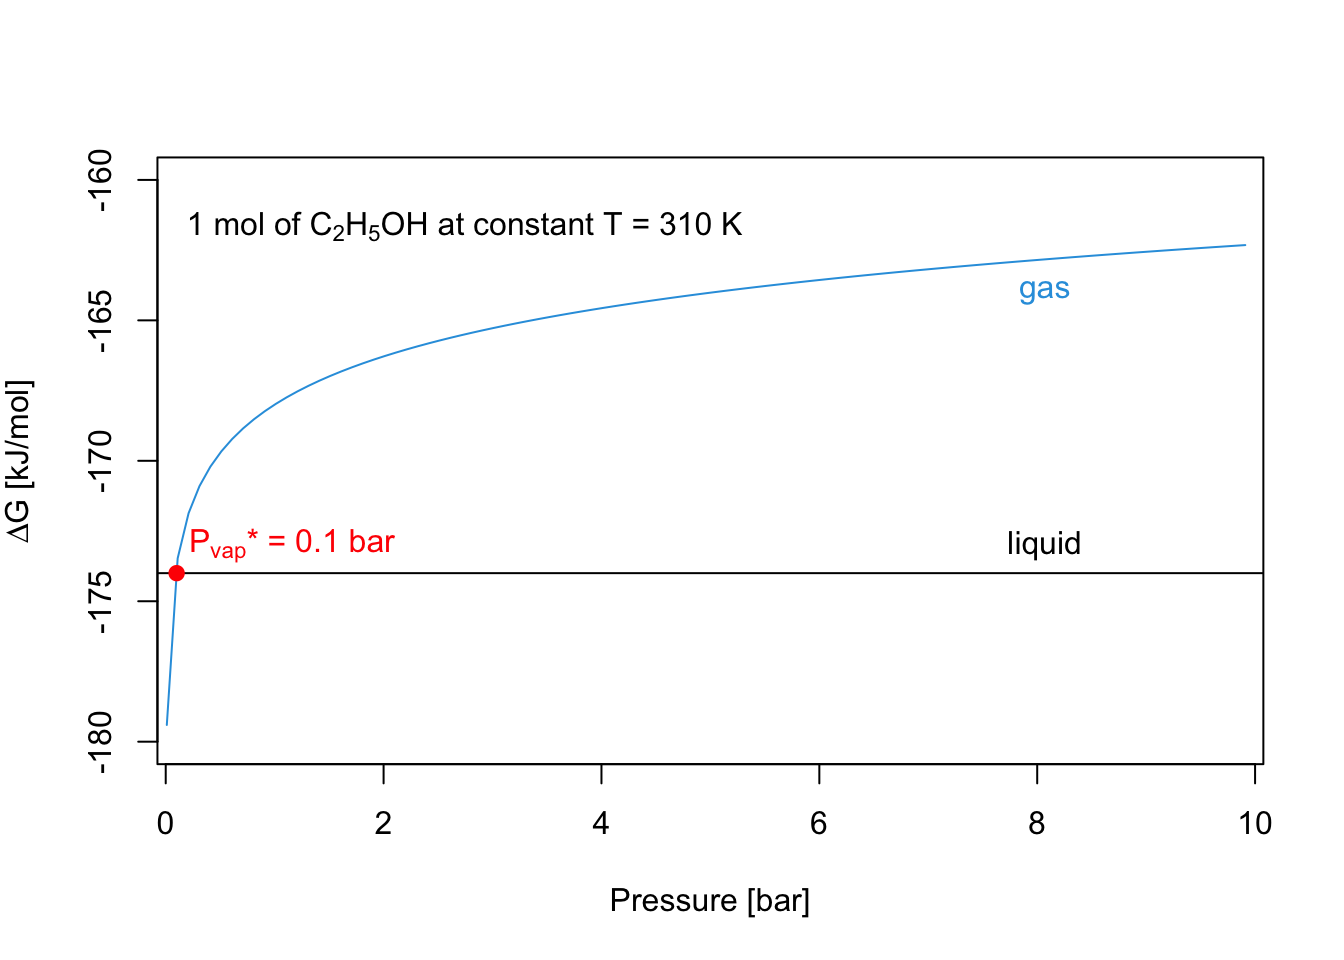
\includegraphics{pchem1_files/figure-latex/gdeppfig-1} 

}

\caption{Dependence of the Gibbs Free Energiy of Formation of Liquid and Gaseous Ethanol at T = 310 K. The Curves Cross at the Vapor Pressure of Liquid Ethanol at this Temperature, which is 0.1 bar.}\label{fig:gdeppfig}
\end{figure}

\hypertarget{composition-dependence-of-delta-g}{%
\section{\texorpdfstring{Composition Dependence of \(\Delta G\)}{Composition Dependence of \textbackslash Delta G}}\label{composition-dependence-of-delta-g}}

\[
\left(\frac{\partial G}{\partial n_i} \right)_{T,P}=\mu_i
\]

The third and final coefficient gives the chemical potential as the dependence of \(G\) on the chemical composition at constant \(T\) and \(P\). Similarly to the previous cases, we can take the definition of the coefficient and integrate it directly between the initial and final stages of a reaction. If we consider a reaction product, pure substance \(i\), at the beginning of the reaction there will be no moles of it \(n_i=0\), and consequently \(G=0\).\footnote{For reactants, the same situation usually applies but in reverse. More complicated cases where the reaction does not consume all reactants are possible, but insignificant for the following treatment.} We can then integrate the left-hand side between zero and the number of moles of product at the end of the reaction, \(n\), and the right-hand side between zero and the Gibbs free energy of the product, \(G\). The integral will become:

\begin{equation}
\int_0^G d G = \int_0^n \mu^* dn,
\label{eq:dgconstn}
\end{equation}

where \(\mu^*\) indicates the chemical potential of a pure substance, which is independent on the number of moles by definition. As such, eq. \eqref{eq:dgconstn} becomes:

\begin{equation}
\int_0^G d G = \mu^* \int_0^n dn \quad \rightarrow \quad G = \mu^* n \quad \rightarrow \quad \mu^* = \frac{G}{n},
\label{eq:dgconstn1}
\end{equation}

which gives a straightforward interpretation of the chemical potential of a pure substance as the molar Gibbs free energy.

We can start from eq. \eqref{eq:dgconsttpintegral2} and write for a pure substance that is brought from \(P_i=P^{-\kern-6pt{\ominus}\kern-6pt-}\) to \(P_f=P\) at constant \(T\):

\begin{equation}
G - G^{-\kern-6pt{\ominus}\kern-6pt-}= nRT \ln \frac{P}{P^{-\kern-6pt{\ominus}\kern-6pt-}},
\label{eq:dgconstn2}
\end{equation}

dividing both sides by \(n\), we obtain:

\begin{equation}
\frac{G}{n} - \frac{G^{-\kern-6pt{\ominus}\kern-6pt-}}{n} = RT \ln \frac{P}{P^{-\kern-6pt{\ominus}\kern-6pt-}},
\label{eq:dgconstn3}
\end{equation}

which, for a pure substance at \(P^{-\kern-6pt{\ominus}\kern-6pt-}= 1 \;\text{bar}\), becomes:

\begin{equation}
\mu^* = \mu^{-\kern-6pt{\ominus}\kern-6pt-}+ RT \ln P.
\label{eq:dgconstn4}
\end{equation}

Notice that, while we use the pressure of the gas inside the logarithm in eq. \eqref{eq:dgconstn4}, the quantity is formally divided by the standard pressure \(P^{-\kern-6pt{\ominus}\kern-6pt-}= 1 \;\text{bar}\), and therefore it is a dimensionless quantity, as it should be. For simplicity of notation, however, we will omit the division by \(P^{-\kern-6pt{\ominus}\kern-6pt-}\) in the remaining of this textbook, especially wherever it does not create confusion.
Let's now consider a mixture of ideal gases, and let's try to find out whether the chemical potential of a pure gas inside the mixture, \(\mu_i^{\text{mixture}}\), is the same as its chemical potential outside the mixture, \(\mu^*\).
To do so, we can use eq. \eqref{eq:dgconstn4} and replace the pressure \(P\) with the partial pressure \(P_i\):

\begin{equation}
\mu_i^{\text{mixture}} = \mu_i^{-\kern-6pt{\ominus}\kern-6pt-}+ RT \ln P_i,
\label{eq:dgconstn5}
\end{equation}

where the partial pressure \(P_i\) can be obtained from the simple relation that is known as \textbf{Dalton's Law}:

\begin{equation}
P_i = y_i P,
\label{eq:daltonlaw}
\end{equation}

with \(y_i\) being the concentration of gas \(i\) measured as a mole fraction in the gas phase \(y_i=\frac{n_i}{n_{\text{TOT}}} < 1\). Replacing eq. \eqref{eq:daltonlaw} into eq. \eqref{eq:dgconstn5}, we obtain:

\begin{equation}
\begin{aligned}
\mu_i^{\text{mixture}} &= \mu_i^{-\kern-6pt{\ominus}\kern-6pt-}+ RT \ln (y_i P) \\
 &= \underbrace{\mu_i^{-\kern-6pt{\ominus}\kern-6pt-}+ RT \ln P}_{\mu_i^*} + RT \ln y_i,
\end{aligned}
\label{eq:dgconstn6}
\end{equation}

which then reduces to the following equation:

\begin{equation}
\mu_i^{\text{mixture}} = \mu_i^* + RT \ln y_i.
\label{eq:dgconstn7}
\end{equation}

Analyzing eq. \eqref{eq:dgconstn7}, we can immediately see that, since \(y_i < 1\):

\begin{equation}
\mu_i^{\text{mixture}} < \mu_i^*,
\label{eq:dgconstn8}
\end{equation}

or, in other words, the chemical potential of a substance in the mixture is always lower than the chemical potential of the pure substance. If we consider a process where we start from two separate pure ideal gases and finish with a mixture of the two, we can calculate the change in Gibbs free energy due to the mixing process with:

\begin{equation}
\Delta_{\text{mixing}} G = \sum n_i \left( \mu_i^{\text{mixture}} - \mu_i^* \right)  < 0,
\label{eq:dgconstn9}
\end{equation}

or, in other words, the process is spontaneous under all circumstances, and pure ideal gases will always mix.

\renewcommand*{\standardstate}{{-\kern-6pt{\ominus}\kern-6pt-}}

\hypertarget{ChemicalEquilibrium}{%
\chapter{Chemical Equilibrium}\label{ChemicalEquilibrium}}

\hypertarget{reaction-quotient-and-equilibrium-constant}{%
\section{Reaction Quotient and Equilibrium Constant}\label{reaction-quotient-and-equilibrium-constant}}

Let's consider a prototypical reaction at constant \(T,P\):

\begin{equation}
 a\mathrm{A} + b\mathrm{B} \rightarrow c\mathrm{C} + d\mathrm{D} 
\label{eq:reaction4}
\end{equation}

The Gibbs free energy of the reaction is defined as:

\begin{equation}
\Delta_{\text{rxn}} G = G_{\text{products}} - G_{\text{reactants}} = G^{\text{C}} + G^{\text{D}} - G^{\text{A}}-G^{\text{B}},
\label{eq:chemeq1}
\end{equation}

and replacing the absolute Gibbs free energies with the chemical potentials \(\mu_i\), we obtain:

\begin{equation}
\Delta_{\text{rxn}} G = c \mu_{\text{C}} + d \mu_{\text{D}} - a \mu_{\text{A}}- b\mu_{\text{B}}.
\label{eq:chemeq2}
\end{equation}

Assuming the reaction is happening in the gas phase, we can then use eq. \eqref{eq:dgconstn5} to replace the chemical potentials with their value in the reaction mixture, as:

\begin{equation}
\begin{aligned}
\mkern-60mu \Delta_{\text{rxn}} G =& \; c (\mu_{\text{C}}^{-\kern-6pt{\ominus}\kern-6pt-}+RT \ln P_{\text{C}}) + d (\mu_{\text{D}}^{-\kern-6pt{\ominus}\kern-6pt-}+RT \ln P_{\text{D}}) +\\ & - a (\mu_{\text{A}}^{-\kern-6pt{\ominus}\kern-6pt-}+RT \ln P_{\text{A}}) - b (\mu_{\text{B}}^{-\kern-6pt{\ominus}\kern-6pt-}+RT \ln P_{\text{B}}) \\
  =& \; \underbrace{c \mu_{\text{C}}^{-\kern-6pt{\ominus}\kern-6pt-}+ d \mu_{\text{D}}^{-\kern-6pt{\ominus}\kern-6pt-}- a \mu_{\text{A}}^{-\kern-6pt{\ominus}\kern-6pt-}- b\mu_{\text{B}}^{-\kern-6pt{\ominus}\kern-6pt-}}_{\Delta_{\text{rxn}} G^{-\kern-6pt{\ominus}\kern-6pt-}}  +RT \ln \frac{P_{\text{C}}^c \cdot P_{\text{D}}^d}{P_{\text{A}}^a \cdot P_{\text{B}}^b}.
\end{aligned}
\label{eq:chemeq3}
\end{equation}

We can define a new quantity called the \emph{reaction quotient} as a function of the partial pressures of each substance:\footnote{Notice that since we used eq. \eqref{eq:dgconstn4} to derive the reaction quotient, the partial pressures inside it are always dimensionless since they are divided by \(P^{-\kern-6pt{\ominus}\kern-6pt-}\).}

\begin{equation}
Q_P = \frac{P_{\text{C}}^c \cdot P_{\text{D}}^d}{P_{\text{A}}^a \cdot P_{\text{B}}^b},
\label{eq:chemeq4}
\end{equation}

and we can then simply rewrite eq. \eqref{eq:chemeq3} using eq. \eqref{eq:chemeq4} as:

\begin{equation}
\Delta_{\text{rxn}} G = \Delta_{\text{rxn}} G^{-\kern-6pt{\ominus}\kern-6pt-}+ RT \ln Q_P.
\label{eq:chemeq5}
\end{equation}

This equation tells us that the sign of \(\Delta_{\text{rxn}} G\) is influenced by the reaction quotient \(Q_P\). For a spontaneous reaction at the beginning, the partial pressures of the reactants are much higher than the partial pressures of the products, therefore \(Q_P \ll 1\) and \(\Delta_{\text{rxn}} G < 0\), as we expect. As the reaction proceeds, the partial pressures of the products will increase, while the partial pressures of the reactants will decrease. Consequently, both \(Q_P\) and \(\Delta_{\text{rxn}} G\) will increase. The reaction will completely stop when \(\Delta_{\text{rxn}} G = 0\), which is the chemical equilibrium point. At the reaction equilibrium:

\begin{equation}
\Delta_{\text{rxn}} G = 0 = \Delta_{\text{rxn}} G^{-\kern-6pt{\ominus}\kern-6pt-}+ RT \ln K_P,
\label{eq:chemeq6}
\end{equation}

where we have defined a new quantity called \textbf{equilibrium constant}, as the value the reaction quotient assumes when the reaction reaches equilibrium, and we have denoted it with the symbol \(K_P\).\footnote{The subscript \(P\) refers to the fact that the equilibrium constant is measured in terms of partial pressures.} From eq. \eqref{eq:chemeq6} we can derive the following fundamental equation on the standard Gibbs free energy of reaction:

\begin{equation}
\Delta_{\text{rxn}} G^{-\kern-6pt{\ominus}\kern-6pt-}= - RT \ln K_P.
\label{eq:chemeqdg0}
\end{equation}

To extend the concept of \(K_P\) beyond the four species in the prototypical reaction \eqref{eq:reaction4}, we can use the product of a series symbol \(\left( \prod_i \right)\), and write:

\begin{equation}
K_P=\prod_i P_{i,\text{eq}}^{\nu_i},
\label{eq:kpdef}
\end{equation}

where \(P_{i,\text{eq}}\) are the partial pressure of each species at equilibrium. Eq. \eqref{eq:kpdef} is in principle valid for ideal gases only. However, reaction involving ideal gases are pretty rare. As such, we can further extend the concept of equilibrium constant and write:

\begin{equation}
K_{\text{eq}} =\prod_i a_{i,\text{eq}}^{\nu_i},
\label{eq:kdef}
\end{equation}

where we have replaced the partial pressure at equilibrium, \(P_{i,\text{eq}}\), with a new concept introduced initially by Gilbert Newton Lewis (1875--1946),\footnote{Gilber Lewis is the same scientist that invented the concept of Lewis Structures.} that he termed \textbf{activiy}, and represented by the letter \(a\). For ideal gases, it is clear that \(a_i=P_i/P^{-\kern-6pt{\ominus}\kern-6pt-}\). For non-ideal gases, the activity is equal to the fugacity \(a_i=f_i/P^{-\kern-6pt{\ominus}\kern-6pt-}\), a concept that we will investigate in the next chapter. For pure liquids and solids, the activity is simply \(a_i=1\). For diluted solutions, the activity is equal to a measured concentration (such as, for example, the mole fraction \(x_i\) in the liquid phase, and \(y_i\) in the gas phase, or the molar concentration \([i]/[i]^{-\kern-6pt{\ominus}\kern-6pt-}\) with \([i]^{-\kern-6pt{\ominus}\kern-6pt-}= 1\;\text[mol/L]\)). Finally for concentrated solutions, the activity is related to the measured concentration via an activity coefficient. We will return to the concept of activity in chapter \ref{Solutions}, when we will specifically deal with solutions. For now, it is interesting to use the activity to write the definition of the following two constants:

\begin{equation}
K_y =\prod_i \left( y_{i,\text{eq}} \right)^{\nu_i} \qquad \qquad \qquad \qquad K_C =\left( \prod_i [i]_{\text{eq}}/[i]^{-\kern-6pt{\ominus}\kern-6pt-}\right)^{\nu_i},
\label{eq:kxkcdef}
\end{equation}

which can then be related with \(K_P\) for a mixture of ideal gases using:

\begin{equation}
P_i = y_i P \qquad \qquad \qquad P_i=\frac{n_i}{V}RT=[i]RT,
\label{eq:kxkcdef2}
\end{equation}

which then results in:

\begin{equation}
K_P = K_y\cdot \left(\frac{P}{P^{-\kern-6pt{\ominus}\kern-6pt-}}\right)^{\Delta \nu} \qquad \qquad K_P = K_C \left( \frac{[i]^{-\kern-6pt{\ominus}\kern-6pt-}RT}{P^{-\kern-6pt{\ominus}\kern-6pt-}} \right)^{\Delta \nu},
\label{eq:kxkcdef3}
\end{equation}

with \(\Delta \nu =\sum_i \nu_i\).

Using the general equilibrium constant, \(K_{\text{eq}}\), we can also rewrite the fundamental equation on \(\Delta_{\text{rxn}} G^{-\kern-6pt{\ominus}\kern-6pt-}\) that we derived in eq. \eqref{eq:chemeqdg0} to be applicable at most conditions, as:

\begin{equation}
\Delta_{\text{rxn}} G^{-\kern-6pt{\ominus}\kern-6pt-}= - RT \ln K_{\text{eq}},
\label{eq:chemeqdgG}
\end{equation}

and since \(\Delta_{\text{rxn}} G^{-\kern-6pt{\ominus}\kern-6pt-}\) depends on \(T,P\) and \(\{n_i\}\), it is useful to explore how \(K_{\text{eq}}\) depends on those variables as well.

\hypertarget{temperature-dependence-of-k_texteq}{%
\section{\texorpdfstring{Temperature Dependence of \(K_{\text{eq}}\)}{Temperature Dependence of K\_\{\textbackslash text\{eq\}\}}}\label{temperature-dependence-of-k_texteq}}

To study the temperature dependence of \(K_{\text{eq}}\) we can use eq. \eqref{eq:chemeqdgG} for the general equilibrium constant and write:

\begin{equation}
\ln K_{\text{eq}} = -\frac{\Delta G^{-\kern-6pt{\ominus}\kern-6pt-}}{RT},
\label{eq:kptemp1}
\end{equation}

which we can then differentiate with respect to temperature at constant \(P,\{n_i\}\) on both sides:

\begin{equation}
\left( \frac{\partial \ln K_{\text{eq}}}{\partial T} \right)_{P,\{n_i\}} = -\frac{1}{R}  \left[ \frac{\partial \left( \frac{\Delta G^{-\kern-6pt{\ominus}\kern-6pt-}}{T} \right)}{\partial T} \right]_{P,\{n_i\}},
\label{eq:kptemp2}
\end{equation}

and, using Gibbs-Helmholtz equation (eq. \eqref{eq:gibbshelm}) to simplify the left hand side, becomes:

\begin{equation}
\left( \frac{\partial \ln K_{\text{eq}}}{\partial T} \right)_{P,\{n_i\}} = -\frac{1}{R} \left( -\frac{\Delta H^{-\kern-6pt{\ominus}\kern-6pt-}}{T^2} \right) = \frac{\Delta H^{-\kern-6pt{\ominus}\kern-6pt-}}{RT^2},
\label{eq:kptemp3}
\end{equation}

which gives the dependence of \(\ln K_{\text{eq}}\) on \(T\) that we were looking for. Eq. \eqref{eq:kptemp3} is also called \textbf{van 't Hoff equation},\footnote{named after Jacobus Henricus ``Henry'' van 't Hoff Jr.~(1852--1911).} and it is the mathematical expression of Le Chatelier's principle. The simplest interpretation is as follows:

\begin{itemize}
\tightlist
\item
  For an exothermic reaction (\(\Delta H^{-\kern-6pt{\ominus}\kern-6pt-}< 0\)): \(K_{\text{eq}}\) will decrease as the temperature increases.
\item
  For an endothermic reaction (\(\Delta H^{-\kern-6pt{\ominus}\kern-6pt-}> 0\)): \(K_{\text{eq}}\) will increase as the temperature increases.
\end{itemize}

If we integrate the van 't Hoff equation between two arbitrary points at constant \(P\), and assuming constant \(\Delta H^{-\kern-6pt{\ominus}\kern-6pt-}\), we obtain the following:

\begin{equation}
\int_1^2 d \ln K_{\text{eq}} = \frac{\Delta H^{-\kern-6pt{\ominus}\kern-6pt-}}{R} \int_1^2 \frac{dT}{T^2},
\label{eq:kptemp4}
\end{equation}

which leads to the linear equation:

\begin{equation}
\ln K_{\text{eq}}(2) = \ln K_{\text{eq}}(1) - \frac{\Delta H^{-\kern-6pt{\ominus}\kern-6pt-}}{R} \left( \frac{1}{T_2}-\frac{1}{T_1} \right).
\label{eq:vthoffeqI}
\end{equation}

which is the equation that produces the so-called \textbf{van 't Hoff plots}, from which \(\Delta H^{-\kern-6pt{\ominus}\kern-6pt-}\) can be experimentally determined:

\begin{figure}

{\centering 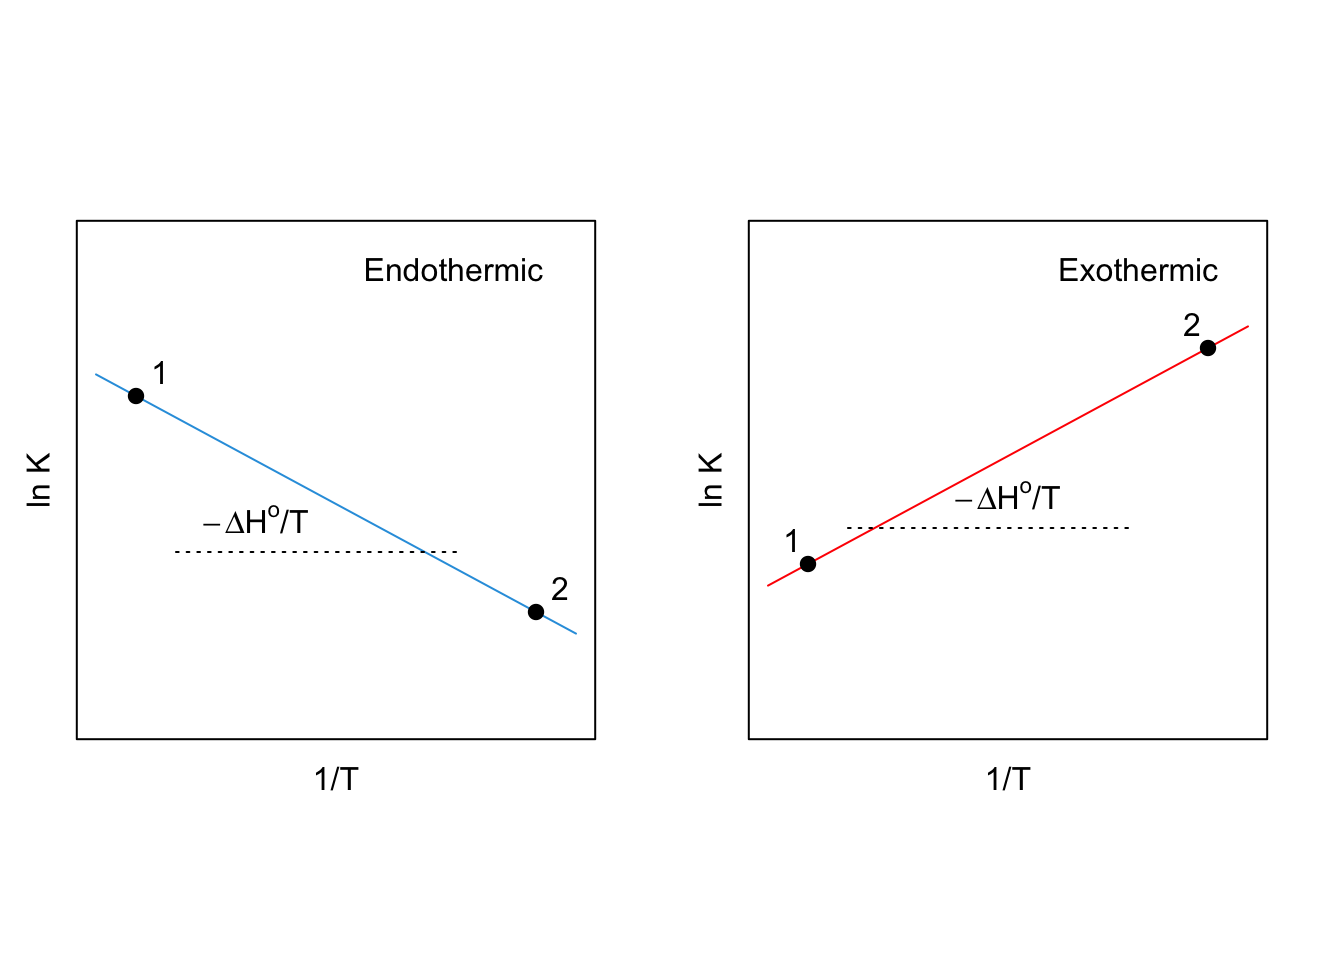
\includegraphics{pchem1_files/figure-latex/vthoffplt-1} 

}

\caption{Van 't Hoff Plots for an Endothermic (Left, Blue) and an Exothermic (Right, Red) Reactions at Constant P.}\label{fig:vthoffplt}
\end{figure}

\hypertarget{pressure-and-composition-dependence-of-k_texteq}{%
\section{\texorpdfstring{Pressure and Composition Dependence of \(K_{\text{eq}}\)}{Pressure and Composition Dependence of K\_\{\textbackslash text\{eq\}\}}}\label{pressure-and-composition-dependence-of-k_texteq}}

While \(K_P\) is independent of both temperature and number of moles for an ideal gas, the same is not necessarily true for the other equilibrium constants.

\begin{equation}
\left( \frac{\partial K_P}{\partial P} \right)_{T,\{n_i\}} = 0 \qquad \qquad \left( \frac{\partial K_P}{\partial n_i}=0 \right)_{T,P}.
\label{eq:kppni}
\end{equation}

For example, it is easy to look at eq. \eqref{eq:kxkcdef3} and determine that \(K_y\) usually depends on \(P\).\footnote{\(K_y\) becomes independent of \(P\) in the particular case where \(\Delta \nu=0\), i.e., for reactions where the total number of moles of reactants is the same as the total number of moles of the products.} Using Dalton's Law, eq. \eqref{eq:daltonlaw}, we can also notice that the equilibrium partial pressures of the reactants and products in a gas-phase reaction can be expressed in terms of their equilibrium mole fractions \(y_i\) and the total pressure \(P\). As such, we can use \(K_y\) to demonstrate that the equilibrium mole fractions will change when \(P\) changes,\footnote{Keep in mind that \(K_P\) will \emph{not} change.} as it is demonstrated by the following exercise.

\begin{quote}
\begin{exercise}
\protect\hypertarget{exr:kpkx}{}{\label{exr:kpkx} }Calculate the mole fraction change for the dissociation of \(\mathrm{Cl}_{2(g)}\) when the pressure is increased from \(P^{-\kern-6pt{\ominus}\kern-6pt-}\) to \(P_f=2.5 \;\text{bar}\) at constant \(T=2\,298\;\mathrm{K}\), knowing that \(\Delta_{\mathrm{f}} G^{-\kern-6pt{\ominus}\kern-6pt-}_{\mathrm{Cl}_{(g)}} = 105.3 \;\text{kJ/mol}\) and \(\Delta_{\mathrm{f}} H^{-\kern-6pt{\ominus}\kern-6pt-}_{\mathrm{Cl}_{(g)}} = 121.3 \;\text{kJ/mol}\), and remembering that both of these values are tabulated at \(T=298\;\text{K}\).

\emph{Solution:} Let's consider the reaction:
\[
\mathrm{Cl}_{2(g)} \rightleftarrows 2 \mathrm{Cl}_{(g)}
\]

We can divide the exercise into two parts. In the first one, we will deal with calculating the equilibrium constant at \(T=2\,298\;\mathrm{K}\) from the data at \(T=298\;\mathrm{K}\). In the second one, we will calculate the change in mole fraction when the pressure is increased from \(P^{-\kern-6pt{\ominus}\kern-6pt-}=1\;\text{bar}\) to \(P_f=2.5 \;\text{bar}\).

\begin{itemize}
\item
  Let's begin the first part by calculating \(\Delta_{\text{rxn}} G^{-\kern-6pt{\ominus}\kern-6pt-}\) and \(\Delta_{\text{rxn}} H^{-\kern-6pt{\ominus}\kern-6pt-}\) from:
  \begin{equation}
  \begin{aligned}
  \Delta_{\text{rxn}} G^{-\kern-6pt{\ominus}\kern-6pt-}&= 2 \Delta_{\text{f}} G^{-\kern-6pt{\ominus}\kern-6pt-}_{\text{Cl}_{(g)}} - \Delta_{\text{f}} G^{-\kern-6pt{\ominus}\kern-6pt-}_{\text{Cl}_{2(g)}} \\
  \Delta_{\text{rxn}} H^{-\kern-6pt{\ominus}\kern-6pt-}&= 2 \Delta_{\text{f}} H^{-\kern-6pt{\ominus}\kern-6pt-}_{\text{Cl}_{(g)}} - \Delta_{\text{f}} H^{-\kern-6pt{\ominus}\kern-6pt-}_{\text{Cl}_{2(g)}},
  \end{aligned}
  \end{equation}
  and since \(\text{Cl}_{2(g)}\) is an element in its most stable form at \(T=298\;\mathrm{K}\), its standard enthalpy and Gibbs free energy of formation are \(\Delta_{\text{f}} H^{-\kern-6pt{\ominus}\kern-6pt-}_{\text{Cl}_{2(g)}} = \Delta_{\text{f}} G^{-\kern-6pt{\ominus}\kern-6pt-}_{\text{Cl}_{2(g)}} = 0\). Therefore:\footnote{Notice how a positive \(\Delta_{\text{rxn}} G^{-\kern-6pt{\ominus}\kern-6pt-}\) indicates that the dissociation of \(\mathrm{CL}_{2(g)}\) is non-spontaneous at \(T=298\;\text{K}\) and \(P=1\;\text{bar}\). As such, we should expect a very small value for \(K_P\).}
  \begin{equation}
  \begin{aligned}
  \Delta_{\text{rxn}} G^{-\kern-6pt{\ominus}\kern-6pt-}&= 2 \cdot 105.3 - 0 = 210.6 \;\text{kJ/mol} \\
  \Delta_{\text{rxn}} H^{-\kern-6pt{\ominus}\kern-6pt-}&= 2 \cdot 121.3 - 0 = 242.6\;\text{kJ/mol}.
  \end{aligned}
  \end{equation}
  Using eq. \eqref{eq:chemeqdg0} to calculate \(K_P (P^{-\kern-6pt{\ominus}\kern-6pt-},298\;\text{K})\), we obtain:\footnote{The results corresponds to \(K_P=1.2\times 10^{-37}\), an incredible miniscule number, as we should expect given the data of \(\Delta_{\text{rxn}} G^{-\kern-6pt{\ominus}\kern-6pt-}\).}
  \begin{equation}
  \ln [ K_P (P^{-\kern-6pt{\ominus}\kern-6pt-},298\;\text{K}) ] =  \frac{ - \Delta_{\text{rxn}} G^{-\kern-6pt{\ominus}\kern-6pt-}}{RT}  =  \frac{-210.6\times10^3}{8.31 \cdot 298} = - 85.0.
  \end{equation}
  We can now use the integrated van 't Hoff equation, eq. \eqref{eq:vthoffeqI}, to calculate \(K_P\) at \(T=2\,298\;\text{K}\):
  \begin{equation}
  \begin{aligned}
  \ln [K_P (P^{-\kern-6pt{\ominus}\kern-6pt-},&2\,298\;\text{K})] = \ln [K_P (P^{-\kern-6pt{\ominus}\kern-6pt-},298\;\text{K})] \;+ \\ &-\frac{\Delta_{\text{rxn}} H^{-\kern-6pt{\ominus}\kern-6pt-}}{R} \left(\frac{1}{2\,298}-\frac{1}{298} \right),
  \end{aligned}
  \end{equation}
  which becomes:
  \begin{equation}
  \begin{aligned}
  \ln [K_P (P^{-\kern-6pt{\ominus}\kern-6pt-},&2\,298\;\text{K})] = - 85.0 \;+\\&-\frac{242.6\times 10^{3}}{8.31} \left(\frac{1}{2\,298}-\frac{1}{298} \right) = 0.262\;,
  \end{aligned}
  \end{equation}
  which corresponds to:
  \begin{equation}
  K_P (P^{-\kern-6pt{\ominus}\kern-6pt-},2\,298\;\text{K}) = \exp (0.262)=1.30.
  \end{equation}
\item
  Let's now move to the second part of the exercise, where we increase the pressure from \(1\;\text{bar}\) to \(2.5\;\text{bar}\) at constant \(T=2\,298\;\text{K}\). We start by writing the definition of \(K_P\) and \(K_y\):
  \begin{equation}
  K_P=\frac{P_\mathrm{Cl_{(g)}}^2}{P_{\mathrm{Cl}_{2(g)}}} \qquad \qquad  K_y=\frac{y_\mathrm{Cl_{(g)}}^2}{y_{\mathrm{Cl}_{2(g)}}},
  \end{equation}
  and using eq. \eqref{eq:kxkcdef3}:
  \begin{equation}
  \begin{aligned}
  \Delta \nu &= 2 - 1 = 1 \\
  K_P &= K_y \cdot \frac{P}{P^{-\kern-6pt{\ominus}\kern-6pt-}} \quad \xrightarrow \qquad K_y=K_P \left( \frac{P}{P^{-\kern-6pt{\ominus}\kern-6pt-}} \right)^{-1},
  \end{aligned}
  \end{equation}
  we can calculate the initial \(K_y\) at \(P_i=P^{-\kern-6pt{\ominus}\kern-6pt-}\), using:
  \begin{equation}
  K_y (P^{-\kern-6pt{\ominus}\kern-6pt-},2\,298\;\text{K}) = 1.30 =\frac{1.30}{1}.
  \end{equation}
  and calculate the initial concentration of \(\mathrm{Cl}_{(g)}\) and \(\mathrm{Cl}_{(g)}\) at \(P^{-\kern-6pt{\ominus}\kern-6pt-}\), recalling that \(y_{\mathrm{Cl}_{2(g)}}=1-y_{\mathrm{Cl}_{(g)}}:\)
  \begin{equation}
  K_y (P_i,2\,298\;\text{K})=\frac{\left(y^i_{\mathrm{Cl}_{(g)}}\right)^2}{y^i_{\mathrm{Cl}_{(g)}}} = 1.30.
  \end{equation}
  Solving the quadratic equation, we obtain one negative answer---which is unphysical---,\footnote{Concentration cannot be negative.} and:
  \begin{equation}
  y_{\mathrm{Cl}_{(g)}}^i= 0.662 \quad \xrightarrow \qquad y_{\mathrm{Cl}_{2(g)}}^i=1-0.662 = 0.338.
  \end{equation}
  At the end of the process, \(P_f=2.5\;\text{bar}\), and we obtain:
  \begin{equation}
  K_y (P_f,2\,298\;\text{K}) = 0.520 = K_P \frac{P^{-\kern-6pt{\ominus}\kern-6pt-}}{P_f} = \frac{1.30}{2.5},
  \end{equation}
  and, using the same technique used before to solve the quadratic equation:
  \begin{equation}
  K_y (P_f,2\,298\;\text{K})=\frac{\left(y^f_{\mathrm{Cl}_{(g)}}\right)^2}{y^f_{\mathrm{Cl}_{(g)}}} = 0.520,
  \end{equation}
  gives:
  \begin{equation}
  y_{\mathrm{Cl}_{(g)}}^f=0.507 \quad \xrightarrow \qquad y_{\mathrm{Cl}_{2(g)}}^i=1-0.507 = 0.493.
  \end{equation}
  To summarize, when we increase the pressure from \(1\;\text{bar}\) to \(2.5\;\text{bar}\) at \(T=2\,298\;\text{K}\), the equilibrium constant in terms of the mole fraction decreases from \(K_y(P^{-\kern-6pt{\ominus}\kern-6pt-},2\,298\;\text{K})=1.30\) to \(K_y(P_f=2.5\;\text{bar},2\,298\;\text{K})=0.520\). This reduction is causing a shift of the equilibrium towards the reactants, with the concentration of \(\text{Cl}_{2(g)}\) increasing from \(y_{\text{Cl}_{2(g)}}^i = 0.338\) to \(y_{\text{Cl}_{2(g)}}^f = 0.493\) and the concentration of \(\text{Cl}_{(g)}\) decreasing from \(y_{\text{Cl}_{2(g)}}^i = 0.662\) to \(y_{\text{Cl}_{(g)}}^f = 0.507\).
\end{itemize}
\end{exercise}
\end{quote}

The dependence of \(K_{\text{eq}}\) on \(P\) highlighted above is another mathematical expression of Le Chatelier's principle, on this occasion, for changes in pressure. The interpretation For a reaction happening in the gas phase is as follows:

\begin{itemize}
\tightlist
\item
  If the total pressure increases, the equilibrium will shift towards the side of the chemical equation that contains the smallest total amount of moles (the equilibrium in exercise \ref{exr:kpkx} shifts toward the reactant).
\end{itemize}

\renewcommand*{\standardstate}{{-\kern-6pt{\ominus}\kern-6pt-}}

\hypertarget{RealGases}{%
\chapter{Ideal and Non-Ideal Gases}\label{RealGases}}

\hypertarget{the-ideal-gas-equation}{%
\section{The Ideal Gas Equation}\label{the-ideal-gas-equation}}

The concept of an ideal gas is a theoretical construct that allows for straightforward treatment and interpretation of gases' behavior. As such, the ideal gas is a simplified \emph{model} that we use to understand nature, and it does not correspond to any real system. The following two assumptions define the ideal gas model:

\begin{quote}
\begin{definition}
\protect\hypertarget{def:iedalgasdef}{}{\label{def:iedalgasdef} }

\begin{itemize}
\tightlist
\item
  The particles that compose an ideal gas do not occupy any volume.
\item
  The particles that compose an ideal gas do not interact with each other.
\end{itemize}
\end{definition}
\end{quote}

Because of its simplicity, the ideal gas model has been the historical foundation of thermodynamics and of science in general. The first studies of the ideal gas behavior date back to the seventeenth century, and the scientists that performed them are among the founders of modern science.

\hypertarget{boyles-law}{%
\subsection{Boyle's Law}\label{boyles-law}}

In 1662 Robert Boyle (1627--1691) found that the pressure and the volume of an ideal gas are inversely related at constant temperature. Boyle's Law has the following mathematical description:

\begin{equation}
P\propto\frac{1}{V}\quad\text{at const.}\;T,
\label{eq:boylelaw1}
\end{equation}

or, in other terms:

\begin{equation}
PV=k_1\quad\text{at const.}\;T,
\label{eq:boylelaw2}
\end{equation}

which results in the familiar \(PV\) plots of Figure \ref{fig:FigPVideal}. As we already discussed in chapter \ref{ZerothLaw}, each of the curves in Figure \ref{fig:FigPVideal} is obtained at constant temperature, and it is therefore called \emph{``isotherm.''}

\begin{figure}

{\centering 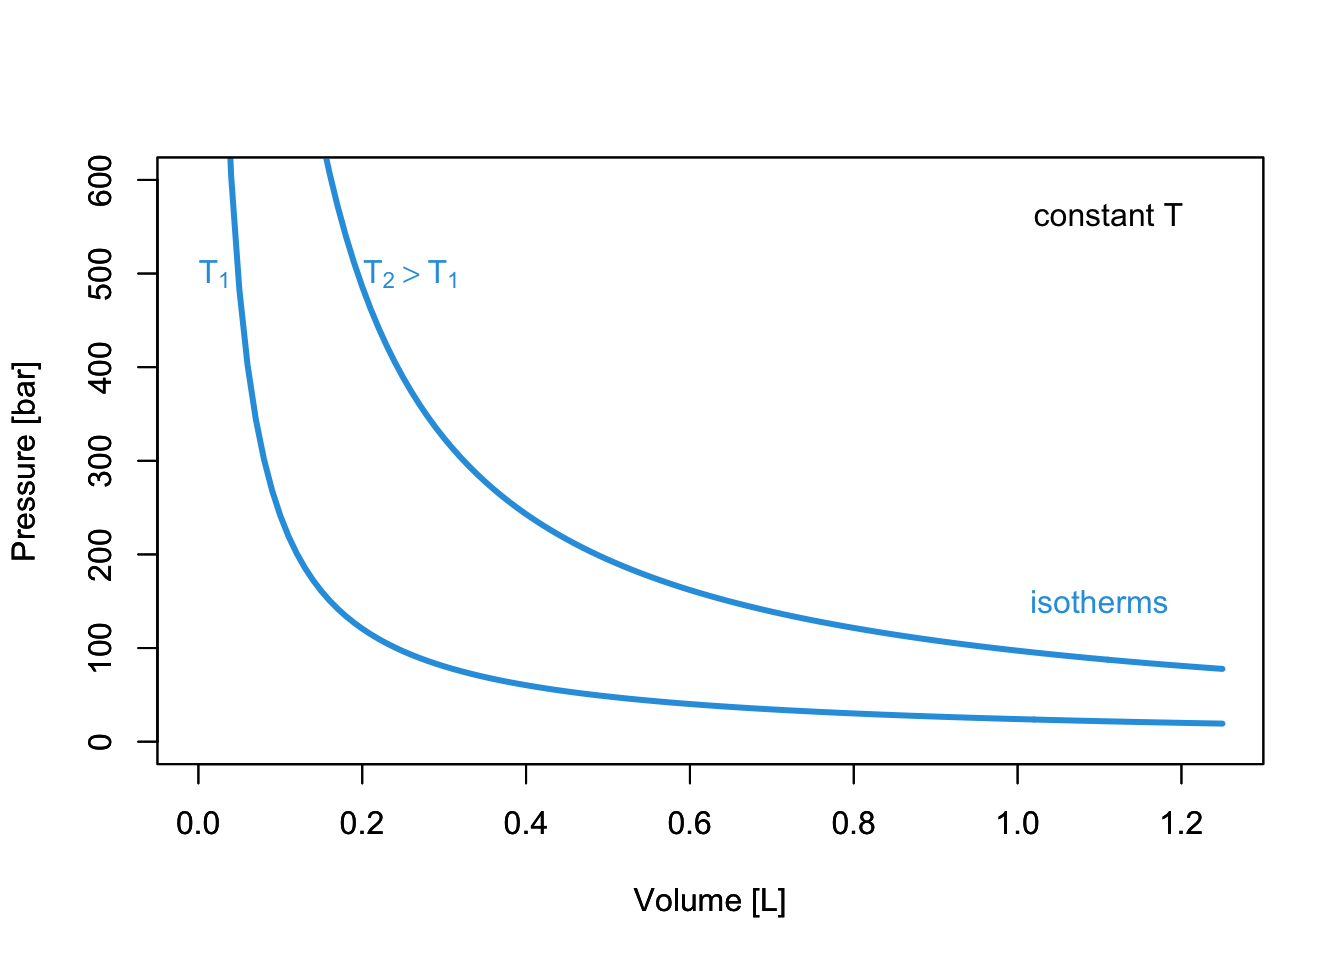
\includegraphics[width=0.7\linewidth]{pchem1_files/figure-latex/FigPVideal-1} 

}

\caption{PV-Diagram of an ideal Gas.}\label{fig:FigPVideal}
\end{figure}

\hypertarget{charless-and-gay-lussacs-laws}{%
\subsection{Charles's and Gay-Lussac's Laws}\label{charless-and-gay-lussacs-laws}}

It took scientists more than a century to expand Boyle's work and study the relationship between volume and temperature. In 1787 Jacques Alexandre César Charles (1746--1823) wrote the relationship known as Charles's Law:

\begin{equation}
V\propto T\quad\text{at const.}\;P,
\label{eq:charleslaw1}
\end{equation}

or, in other terms:

\begin{equation}
V=k_2 T\quad\text{at const.}\;P,
\label{eq:charleslaw2}
\end{equation}

which results in the plots of Figure \ref{fig:FigTVideal}. Each of the curves is obtained at constant pressure, and it is termed \emph{``isobar.''}

\begin{figure}

{\centering 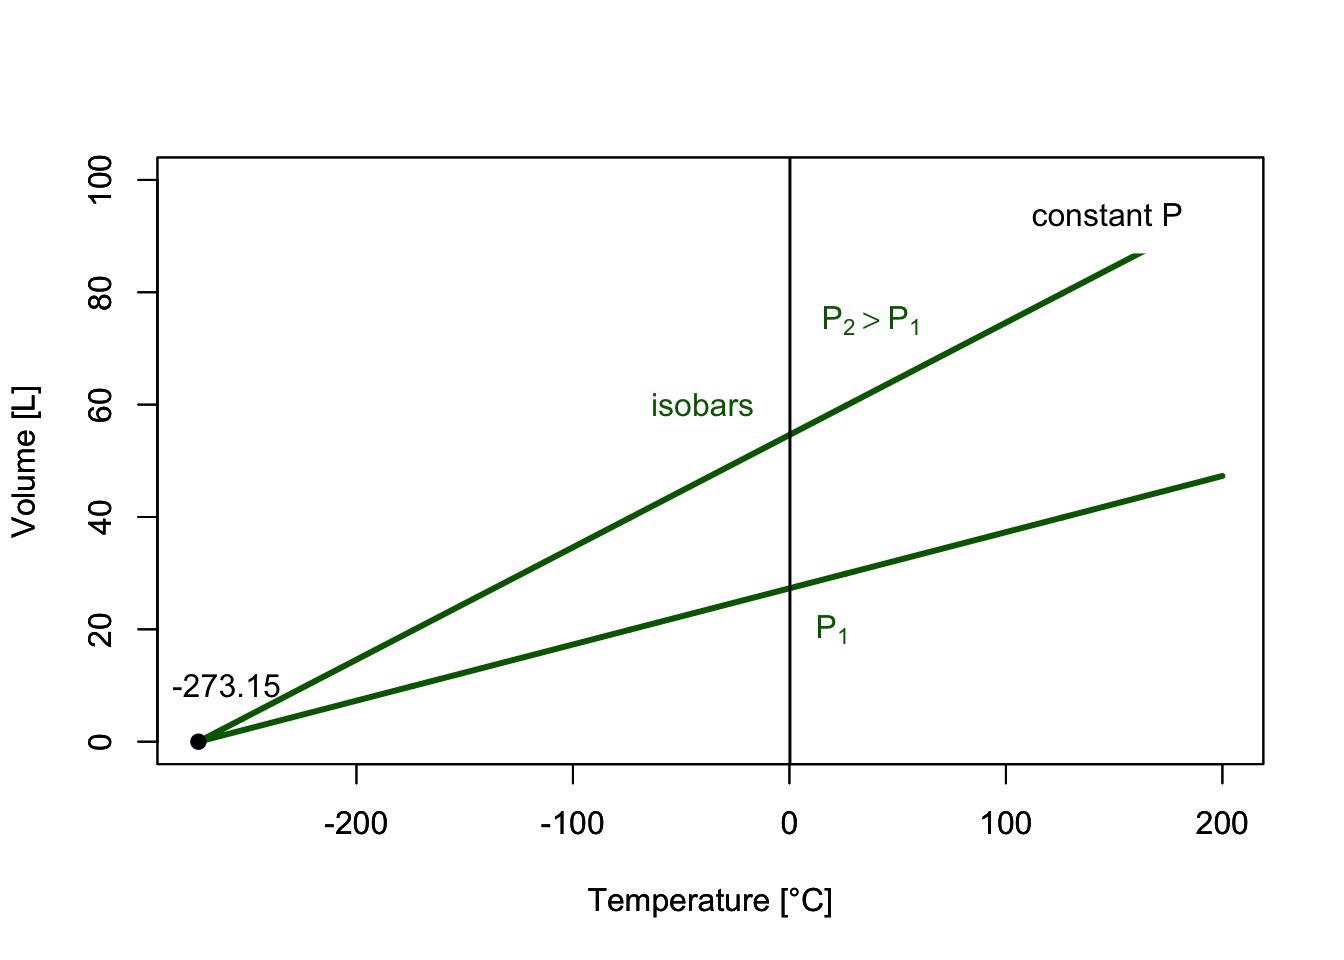
\includegraphics[width=0.7\linewidth]{pchem1_files/figure-latex/FigTVideal-1} 

}

\caption{VT-Diagram of an ideal Gas.}\label{fig:FigTVideal}
\end{figure}

The interesting thing about isobars is that each line seems to converge to a specific point along the temperature line when we extrapolate them to \(V\rightarrow 0\). This led to the introduction of the absolute temperature scale, suggesting that the temperature will never get smaller than \(-273.15^\circ\mathrm{C}\).

It took an additional 21 years to write a formal relationship between pressure and temperature. The following relationships were proposed by Joseph Louis Gay-Lussac (1778--1850) in 1808:

\begin{equation}
P\propto T\quad\text{at const.}\;V,
\label{eq:gaylussac1}
\end{equation}

or, in other terms:

\begin{equation}
P=k_3 T\quad\text{at const.}\;V,
\label{eq:gaylussac2}
\end{equation}

which results in the plots of Figure \ref{fig:FigTPideal}. Each of the curves is obtained at constant volume, and it is termed \emph{``isochor.''}

\begin{figure}

{\centering 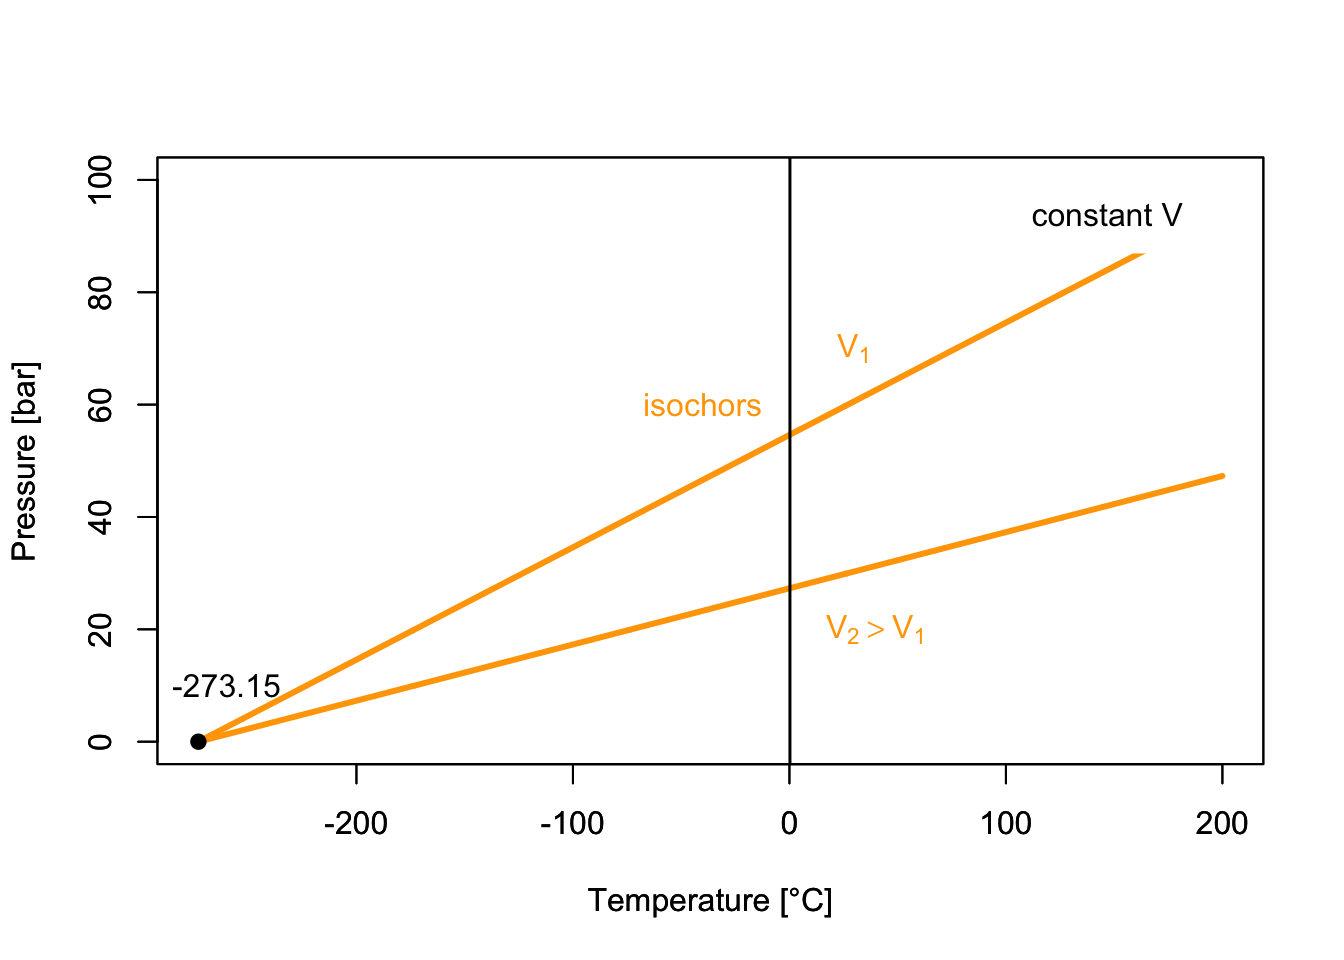
\includegraphics[width=0.7\linewidth]{pchem1_files/figure-latex/FigTPideal-1} 

}

\caption{PT-Diagram of an ideal Gas.}\label{fig:FigTPideal}
\end{figure}

\hypertarget{avogadros-law}{%
\subsection{Avogadro's Law}\label{avogadros-law}}

Ten years later, Amedeo Avogadro (1776--1856) discovered a seemingly unrelated principle by studying the composition of matter. His Avogadro's Law encodes the relationship between the number of moles in an ideal gas and its volume as:

\begin{equation}
V\propto n\quad\text{at const.}\;P,T,
\label{eq:avogadrolaw1}
\end{equation}

or in other terms:

\begin{equation}
V=k_4 n\quad\text{at const.}\;P,T,
\label{eq:avogadrolaw2}
\end{equation}

\hypertarget{the-ideal-gas-law}{%
\subsection{The ideal gas Law}\label{the-ideal-gas-law}}

Despite all of the ingredients being available for more than 20 years, it's only in 1834 that Benoît Paul Émile Clapeyron (1799--1864) was finally able to combine them into what is now known as the \textbf{ideal gas Law}. Using the same formulas obtained above, we can write:

\begin{equation}
PV=\underbrace{k_3 T}_{\text{from Gay-Lussac's}} \cdot \underbrace{k_4 n,}_{\text{from Avogadro's}}
\label{eq:ideallaw1}
\end{equation}

which by renaming the product of the two constants \(k_3\) and \(k_4\) as \(R\), becomes:

\begin{equation}
PV=nRT
\label{eq:ideallaw2}
\end{equation}

The value of the constant \(R\) can be determined experimentally by measuring the volume that 1 mol of an ideal gas occupies at a constant temperature (e.g., at \(T=0^\circ\mathrm{C}\)) and a constant pressure (e.g., atmospheric pressure \(P=1\;\mathrm{atm}\)). At those conditions, the volume is measured at 22.4 L, resulting in the following value of \(R\):

\begin{equation}
R=\frac{VP}{nT}=\frac{22.4 \cdot 1}{1 \cdot 273}=0.082 \;\frac{\text{L atm}}{\text{mol K}},
\label{eq:ideallaw3}
\end{equation}

which a simple conversion to SI units transforms into:

\begin{equation}
R=8.31\;\frac{\text{J}}{\text{mol K}}.
\label{eq:RvalueSI}
\end{equation}

\hypertarget{behaviors-of-non-ideal-gases}{%
\section{Behaviors of Non-Ideal Gases}\label{behaviors-of-non-ideal-gases}}

Non-ideal gases (sometimes also referred to as ``real gases''), do not behave as ideal gases because at least one of the assumptions in definition \ref{def:iedalgasdef} is violated. What characterizes non-ideal gases is that there is no unique equation that we can use to describe their behavior. For this reason, we have a plethora of several experimental models, none of which is superior to the other. The van der Waals (vdW) equation is the only model that we will analyze in detail because of its simple interpretation. However, it is far from universal, and for several non-ideal gases, it is severely inaccurate. Other popular non-ideal gases equations are the Clausius equation, the virial equation, the Redlich--Kwong equation and several others.\footnote{For more information on empirical equations for non-ideal gases see \href{https://en.wikipedia.org/wiki/Real_gas}{this Wikipedia page}.}

\hypertarget{the-van-der-waals-equation}{%
\subsection{The van der Waals equation}\label{the-van-der-waals-equation}}

One of the simplest empirical equation that describes non-ideal gases was obtained in 1873 by Johannes Diderik van der Waals (1837--1923). The vdW equation includes two empirical parameters (\(a\) and \(b\)) with different values for different non-ideal gases. Each of the parameters corresponds to a correction for the breaking of one of the two conditions that define the ideal gas behavior (definition \ref{def:iedalgasdef}). The vdW equation is obtained from the ideal gas equation performing the following simple substitutions:

\begin{equation}
\begin{aligned}
P & \;\rightarrow\;\left( P + \frac{a}{\overline{V}^2} \right)\\
\overline{V} & \;\rightarrow\;\left( \overline{V} - b\right),\\
\end{aligned}
\label{eq:vdWeq1}
\end{equation}

which results in:

\begin{equation}
\begin{aligned}
P\overline{V} &=RT \; \rightarrow \; \left( P + \frac{a}{\overline{V}^2} \right)\left( \overline{V} - b\right)=RT\\
P &=\frac{RT}{\overline{V} - b}-\frac{a}{\overline{V}^2}.
\end{aligned}
\label{eq:vdWeq2}
\end{equation}

The parameter \(a\) accounts for the presence of intermolecular interactions, while the parameter \(b\) accounts for the non-negligible volume of the gas molecules. Despite the parameters having simple interpretations, their values for each gas must be determined experimentally. Values for these parameters for some significant non-ideal gas are reported below:

\scriptsize

\begin{longtable}[]{@{}lcc@{}}
\toprule
\begin{minipage}[b]{(\columnwidth - 2\tabcolsep) * \real{0.12}}\raggedright
\strut
\end{minipage} & \begin{minipage}[b]{(\columnwidth - 2\tabcolsep) * \real{0.50}}\centering
\(a \left[ \frac{\mathrm{L}^2\mathrm{bar}}{\mathrm{mol}^2} \right]\)\strut
\end{minipage} & \begin{minipage}[b]{(\columnwidth - 2\tabcolsep) * \real{0.38}}\centering
\(b \left[ \frac{\mathrm{L}}{\mathrm{mol}} \right]\)\strut
\end{minipage}\tabularnewline
\midrule
\endhead
\begin{minipage}[t]{(\columnwidth - 2\tabcolsep) * \real{0.12}}\raggedright
Ammonia\strut
\end{minipage} & \begin{minipage}[t]{(\columnwidth - 2\tabcolsep) * \real{0.50}}\centering
4.225\strut
\end{minipage} & \begin{minipage}[t]{(\columnwidth - 2\tabcolsep) * \real{0.38}}\centering
0.0371\strut
\end{minipage}\tabularnewline
\begin{minipage}[t]{(\columnwidth - 2\tabcolsep) * \real{0.12}}\raggedright
Argon\strut
\end{minipage} & \begin{minipage}[t]{(\columnwidth - 2\tabcolsep) * \real{0.50}}\centering
1.355\strut
\end{minipage} & \begin{minipage}[t]{(\columnwidth - 2\tabcolsep) * \real{0.38}}\centering
0.03201\strut
\end{minipage}\tabularnewline
\begin{minipage}[t]{(\columnwidth - 2\tabcolsep) * \real{0.12}}\raggedright
Carbon dioxide\strut
\end{minipage} & \begin{minipage}[t]{(\columnwidth - 2\tabcolsep) * \real{0.50}}\centering
3.640\strut
\end{minipage} & \begin{minipage}[t]{(\columnwidth - 2\tabcolsep) * \real{0.38}}\centering
0.04267\strut
\end{minipage}\tabularnewline
\begin{minipage}[t]{(\columnwidth - 2\tabcolsep) * \real{0.12}}\raggedright
Carbon monoxide\strut
\end{minipage} & \begin{minipage}[t]{(\columnwidth - 2\tabcolsep) * \real{0.50}}\centering
1.505\strut
\end{minipage} & \begin{minipage}[t]{(\columnwidth - 2\tabcolsep) * \real{0.38}}\centering
0.03985\strut
\end{minipage}\tabularnewline
\begin{minipage}[t]{(\columnwidth - 2\tabcolsep) * \real{0.12}}\raggedright
Chlorine\strut
\end{minipage} & \begin{minipage}[t]{(\columnwidth - 2\tabcolsep) * \real{0.50}}\centering
6.579\strut
\end{minipage} & \begin{minipage}[t]{(\columnwidth - 2\tabcolsep) * \real{0.38}}\centering
0.05622\strut
\end{minipage}\tabularnewline
\begin{minipage}[t]{(\columnwidth - 2\tabcolsep) * \real{0.12}}\raggedright
Freon\strut
\end{minipage} & \begin{minipage}[t]{(\columnwidth - 2\tabcolsep) * \real{0.50}}\centering
10.78\strut
\end{minipage} & \begin{minipage}[t]{(\columnwidth - 2\tabcolsep) * \real{0.38}}\centering
0.0998\strut
\end{minipage}\tabularnewline
\begin{minipage}[t]{(\columnwidth - 2\tabcolsep) * \real{0.12}}\raggedright
Helium\strut
\end{minipage} & \begin{minipage}[t]{(\columnwidth - 2\tabcolsep) * \real{0.50}}\centering
0.0346\strut
\end{minipage} & \begin{minipage}[t]{(\columnwidth - 2\tabcolsep) * \real{0.38}}\centering
0.0238\strut
\end{minipage}\tabularnewline
\begin{minipage}[t]{(\columnwidth - 2\tabcolsep) * \real{0.12}}\raggedright
Hydrogen\strut
\end{minipage} & \begin{minipage}[t]{(\columnwidth - 2\tabcolsep) * \real{0.50}}\centering
0.2476\strut
\end{minipage} & \begin{minipage}[t]{(\columnwidth - 2\tabcolsep) * \real{0.38}}\centering
0.02661\strut
\end{minipage}\tabularnewline
\begin{minipage}[t]{(\columnwidth - 2\tabcolsep) * \real{0.12}}\raggedright
Mercury\strut
\end{minipage} & \begin{minipage}[t]{(\columnwidth - 2\tabcolsep) * \real{0.50}}\centering
8.200\strut
\end{minipage} & \begin{minipage}[t]{(\columnwidth - 2\tabcolsep) * \real{0.38}}\centering
0.01696\strut
\end{minipage}\tabularnewline
\begin{minipage}[t]{(\columnwidth - 2\tabcolsep) * \real{0.12}}\raggedright
Methane\strut
\end{minipage} & \begin{minipage}[t]{(\columnwidth - 2\tabcolsep) * \real{0.50}}\centering
2.283\strut
\end{minipage} & \begin{minipage}[t]{(\columnwidth - 2\tabcolsep) * \real{0.38}}\centering
0.04278\strut
\end{minipage}\tabularnewline
\begin{minipage}[t]{(\columnwidth - 2\tabcolsep) * \real{0.12}}\raggedright
Neon\strut
\end{minipage} & \begin{minipage}[t]{(\columnwidth - 2\tabcolsep) * \real{0.50}}\centering
0.2135\strut
\end{minipage} & \begin{minipage}[t]{(\columnwidth - 2\tabcolsep) * \real{0.38}}\centering
0.01709\strut
\end{minipage}\tabularnewline
\begin{minipage}[t]{(\columnwidth - 2\tabcolsep) * \real{0.12}}\raggedright
Nitrogen\strut
\end{minipage} & \begin{minipage}[t]{(\columnwidth - 2\tabcolsep) * \real{0.50}}\centering
1.370\strut
\end{minipage} & \begin{minipage}[t]{(\columnwidth - 2\tabcolsep) * \real{0.38}}\centering
0.0387\strut
\end{minipage}\tabularnewline
\begin{minipage}[t]{(\columnwidth - 2\tabcolsep) * \real{0.12}}\raggedright
Oxygen\strut
\end{minipage} & \begin{minipage}[t]{(\columnwidth - 2\tabcolsep) * \real{0.50}}\centering
1.382\strut
\end{minipage} & \begin{minipage}[t]{(\columnwidth - 2\tabcolsep) * \real{0.38}}\centering
0.03186\strut
\end{minipage}\tabularnewline
\begin{minipage}[t]{(\columnwidth - 2\tabcolsep) * \real{0.12}}\raggedright
Radon\strut
\end{minipage} & \begin{minipage}[t]{(\columnwidth - 2\tabcolsep) * \real{0.50}}\centering
6.601\strut
\end{minipage} & \begin{minipage}[t]{(\columnwidth - 2\tabcolsep) * \real{0.38}}\centering
0.06239\strut
\end{minipage}\tabularnewline
\begin{minipage}[t]{(\columnwidth - 2\tabcolsep) * \real{0.12}}\raggedright
Xenon\strut
\end{minipage} & \begin{minipage}[t]{(\columnwidth - 2\tabcolsep) * \real{0.50}}\centering
4.250\strut
\end{minipage} & \begin{minipage}[t]{(\columnwidth - 2\tabcolsep) * \real{0.38}}\centering
0.05105\strut
\end{minipage}\tabularnewline
\bottomrule
\end{longtable}

\normalsize

\hypertarget{joulethomson-effect}{%
\subsection{Joule--Thomson effect}\label{joulethomson-effect}}

\begin{figure}

{\centering 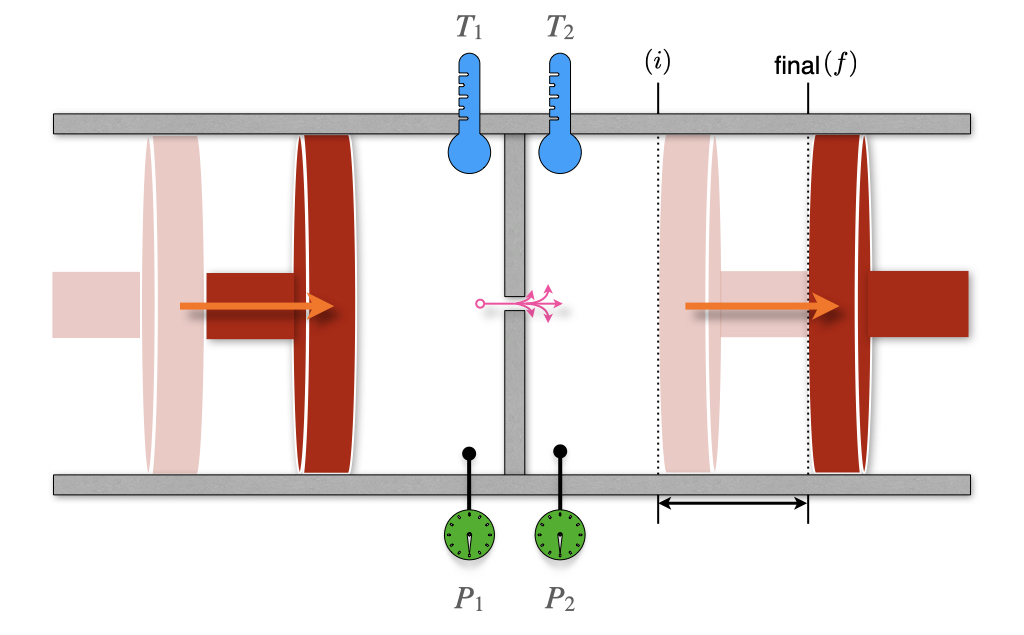
\includegraphics[width=0.8\linewidth]{./img/OEP_Figures.015} 

}

\caption{The Joule–Thomson Experiment.}\label{fig:FigJT}
\end{figure}

We have already met William Thomson, also known as Lord Kelvin, and his seminal work on the second law of thermodynamics. In conjunction with that work, Thomson is famous for developing a sensitive method for measuring the temperature changes related to the expansion of a gas. These experiments improved on the earlier work by James Joule, and Lord Kelvin's improved instrument depicted in Figure \ref{fig:FigJT} is named the Joule--Thomson apparatus. The apparatus is composed of two chambers, each with its own mobile piston. The chambers are connected via a valve or a porous plug. The entire equipment is also thermally isolated from the surroundings. This instrument is a more sensitive version of the Joule expansion apparatus that we already described in section \ref{FirstLaw} (compare with Figure \ref{fig:FigJexp}).

Thomson realized that a gas flowing through an obstruction experience a drop in pressure. If the entire apparatus is insulated, it will not exchange heat with its surroundings (\(Q=0\)), and each transformation will happen at adiabatic conditions. Let's consider an initial condition with 1 mol of gas in the left chamber, occupying a volume \(V_l\), and a completely closed left chamber, for which \(V_r^i=0\). After the process completes, the volume of the right chamber will reduce to \(V_l^f=0\), while the volume of the right chamber will be \(V_r\). Using the first law of thermodynamics, we can write:

\begin{equation}
\Delta U=U_r-U_l=\underbrace{Q}_{=0}+W=W_l+W_r,
\label{eq:JT1}
\end{equation}

with:

\begin{equation}
\begin{aligned}
W_l &=-\int_{V_l}^0 P_l dV = P_l V_l\\
W_r &=-\int_0^{V_r} P_r dV = - P_r V_r.
\end{aligned}
\label{eq:JT2}
\end{equation}

Replacing \eqref{eq:JT2} into eq. \eqref{eq:JT1}, results in:

\begin{equation}
\begin{aligned}
U_r-U_l &=P_l V_l-P_r V_r \\
\underbrace{U_r+P_r V_r}_{H_r} &= \underbrace{U_l + P_l V_l}_{H_l},
\end{aligned}
\label{eq:JT3}
\end{equation}

which, replacing the definition of enthalpy \(H=U+PV\), we obtain:

\begin{equation}
\begin{aligned}
H_r &=H_l \\
\Delta H &=0,
\end{aligned}
\label{eq:JT4}
\end{equation}

or, in other words, the process is \textbf{isenthalpic}. Using the total differential of \(H\):

\begin{equation}
dH=\left(\frac{\partial H}{\partial T} \right)_P dT + \left(\frac{\partial H}{\partial P} \right)_T dP = C_P dT + \left(\frac{\partial H}{\partial P} \right)_T dP,
\label{eq:JT5}
\end{equation}

we obtain:

\begin{equation}
\Delta H=\int dH = \int C_P dT + \int \left(\frac{\partial H}{\partial P} \right)_T dP =0,
\label{eq:JT6b}
\end{equation}

or, in purely differential form:

\begin{equation}
dH = C_P dT + \left(\frac{\partial H}{\partial P} \right)_T dP =0,
\label{eq:JT6}
\end{equation}

From eq. \eqref{eq:JT6} we can define a new coefficient, called the \emph{Joule--Thomson coefficient}, \(\mu_{\mathrm{JT}}\), that measures the rate of change of temperature of a gas with respect to pressure in the Joule--Thomson process:

\begin{equation}
\mu_{\mathrm{JT}}=\left( \frac{\partial T}{\partial P} \right)_H=-\frac{1}{C_P} \left( \frac{\partial H}{\partial T} \right)_P
\label{eq:muJT}
\end{equation}

The value of \(\mu_{\mathrm{JT}}\) depends on the type of gas, the temperature and pressure before expansion, and the heat capacity at constant pressure of the gas. The temperature at which \(\mu_{\mathrm{JT}}\) changes sign is called the ``Joule--Thomson inversion temperature.'' Since the pressure decreases during an expansion, \(\partial P\) is negative by definition, and the following possibilities are available for \(\mu_{\mathrm{JT}}\):

\begin{longtable}[]{@{}lcccc@{}}
\toprule
Gas temperature: & \(\partial P\) & \(\mu_{\mathrm{JT}}\) & \(\partial T\) & The gas will:\tabularnewline
\midrule
\endhead
\emph{Below the inversion temperature} & -- & + & -- & cool\tabularnewline
\emph{Above the inversion temperature} & -- & -- & + & warm\tabularnewline
\bottomrule
\end{longtable}

For example, helium has a very low Joule--Thomson inversion temperatures at standard pressure \((T=45\;\text{K})\), and it warms when expanded at constant enthalpy at typical room temperatures. The only other gases that have standard inversion temperature lower than room temperature are hydrogen and neon. On the other hand, nitrogen and oxygen have high inversion temperatures (\(T=621\;\text{K}\) and \(T=764\;\text{K}\), respectively), and they both cool when expanded at room temperature. Therefore, it is possible to use the Joule--Thomson effect in refrigeration processes such as air conditioning.\footnote{Nitrogen and oxygen are the two most abundant gases in the air. A sequence of Joule--Thomson expansions are also used for the industrial liquefaction of air.} As we already discussed in chapter \ref{FirstLaw}, the temperature of an ideal gases stays constant in an adiabatic expansion, therefore its Joule--Thomson coefficient is always equal to zero.

\hypertarget{critical-phenomena}{%
\section{Critical Phenomena}\label{critical-phenomena}}

\hypertarget{compressibility-factors}{%
\subsection{Compressibility factors}\label{compressibility-factors}}

The compressibility factor is a correction coefficient that describes the deviation of a real gas from ideal gas behaviour. It is usually represented with the symbol \(z\), and is calculated as:

\begin{equation}
z=\frac{\overline{V}}{\overline{V}_{\text{ideal}}} = \frac{P \overline{V}}{RT}.
\label{eq:comprdef}
\end{equation}

It is evident from eq. \eqref{eq:comprdef} that the compressibility factor is dependent on the pressure, and for an ideal gas \(z=1\) always. For a non-ideal gas at any given pressure, \(z\) can be higher or lower than one, separating the behavior of non-ideal gases into two possibilities. The dependence of the compressibility factor against pressure is represented for \(\mathrm{H}_2\) and \(\mathrm{CO}_2\) in Figure \ref{fig:FigZb}.

\begin{figure}

{\centering 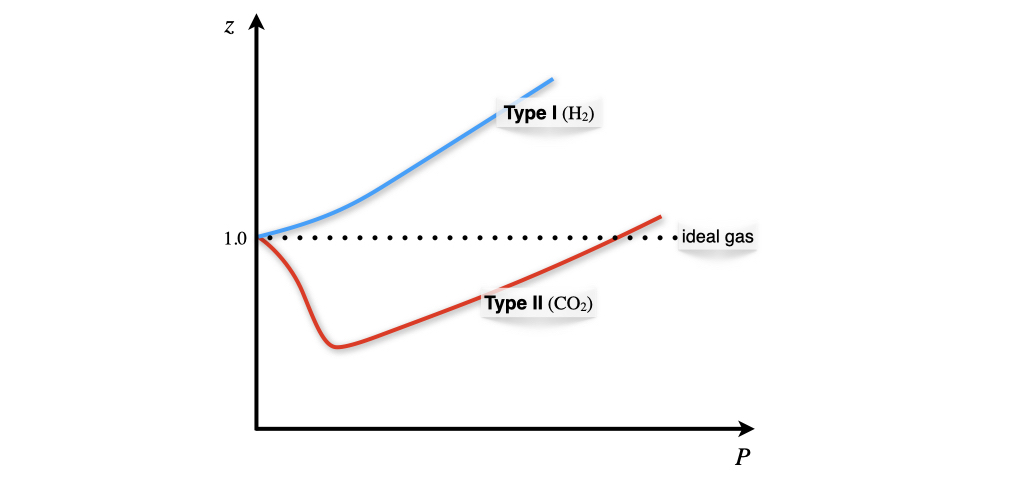
\includegraphics[width=0.8\linewidth]{./img/OEP_Figures.012} 

}

\caption{Non-Ideal Gases Behaviors.}\label{fig:FigZb}
\end{figure}

The two types of possible behaviors are differentiated based on the compressibility factor at \(P\rightarrow 0\). To analyze these situations we can use the vdW equation to calculate the compressibility factor as:

\begin{equation}
z= \frac{\overline{V}}{RT} \left( \frac{RT}{\overline{V}-b} -\frac{a}{\overline{V}^2} \right).
\label{eq:compr1}
\end{equation}

and then we can differentiate this equation at constant temperature with respect to changes in the pressure near \(P=0\), to obtain:

\begin{equation}
\left. \left( \frac{\partial z}{\partial P}\right)_T \right|_{P=0} = \frac{1}{RT} \left( b -\frac{a}{RT} \right).
\label{eq:compr2}
\end{equation}

which is then interpreted as follows:

\begin{itemize}
\tightlist
\item
  \textbf{Type I gases}: \(b>\frac{a}{RT} \; \Rightarrow \; \frac{\partial z}{\partial P} > 0\) \emph{molecular size} dominates (\(\mathrm{H}_2-\)like behavior).
\item
  \textbf{Type II gases}: \(b<\frac{a}{RT} \; \Rightarrow \; \frac{\partial z}{\partial P} < 0\) \emph{attractive forces} dominates (\(\mathrm{CO}_2-\)like behavior).
\end{itemize}

The dependence of the compressibility factor as a function of temperature (Figure \ref{fig:Fig1Zb2}) results in different plots for each of the two types of behavior.

\begin{figure}

{\centering 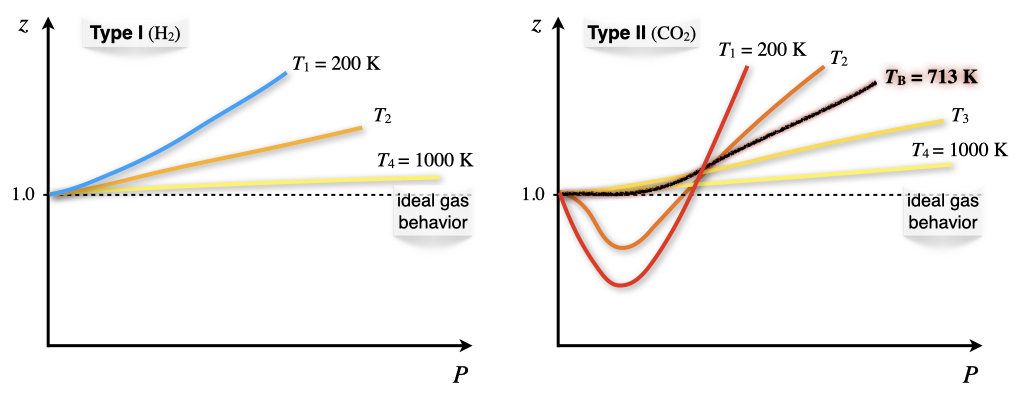
\includegraphics[width=0.9\linewidth]{./img/OEP_Figures.013} 

}

\caption{Temperature Dependence of the Compressibility Factor.}\label{fig:Fig1Zb2}
\end{figure}

Both type I and type II non-ideal gases will approach the ideal gas behavior as \(T\rightarrow \infty\), because \(\frac{1}{RT}\rightarrow 0\) as \(T\rightarrow \infty\). For type II gases, there are three interesting situations:

\begin{itemize}
\tightlist
\item
  At low \(T\): \(b<\frac{a}{RT} \; \Rightarrow \; \frac{\partial z}{\partial P} < 0,\) which is the behavior described above.
\item
  At high \(T\): \(b>\frac{a}{RT} \; \Rightarrow \; \frac{\partial z}{\partial P} > 0,\) which is the same behavior of type I gases.
\item
  At a very specific temperature, inversion will occur (i.e., at \(T=713 \; \mathrm{K}\) for \(\mathrm{CO}_2\)). This temperature is called the \textbf{Boyle temperature}, \(T_{\mathrm{B}}\), and is the temperature at which the attractive and repulsive forces balance out. It can be calculated from the vdW equation, since \(b-\frac{a}{RT_{\mathrm{B}}}=0 \; \Rightarrow \; T_{\mathrm{B}}=\frac{a}{bR}.\) At the Boyle's temperature a type II gas shows ideal gas behavior over a large range of pressure.
\end{itemize}

\hypertarget{phase-diagram-of-a-non-ideal-gas}{%
\subsection{Phase diagram of a non-ideal gas}\label{phase-diagram-of-a-non-ideal-gas}}

\begin{figure}

{\centering 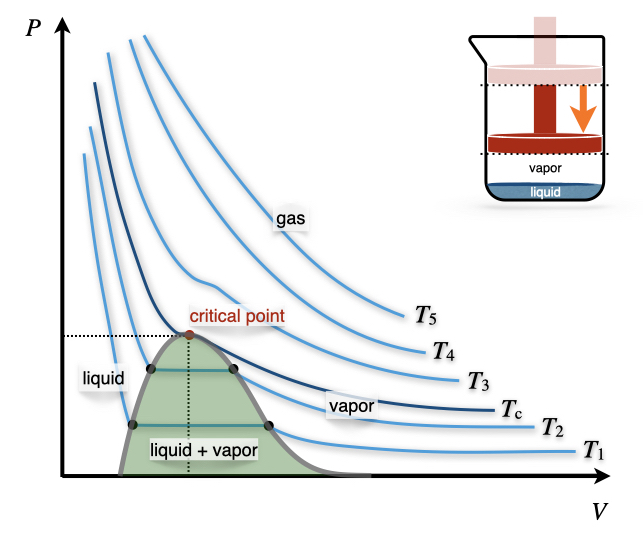
\includegraphics[width=0.6\linewidth]{./img/OEP_Figures.014} 

}

\caption{The Pressure–Volume Diagram of a Non-Ideal Gas.}\label{fig:FigPVni}
\end{figure}

Let's now turn our attention to the \(PV\) phase diagram of a non-ideal gas, reported in Figure \ref{fig:FigPVni}. We can start the analysis from an isotherm at a high temperature. Since every gas will behave as an ideal gas at those conditions, the corresponding isotherms will look similar to those of an ideal gas (\(T_5\) and \(T_4\) in Figure \ref{fig:FigPVni}). Lowering the temperature, we start to see the deviation from ideality getting more prominent (\(T_3\) in Figure \ref{fig:FigPVni}) until we reach a particular temperature called the critical temperature, \(T_c\).

\begin{quote}
\begin{definition}
\protect\hypertarget{def:criticalT}{}{\label{def:criticalT} }\emph{Critical Temperature:} The temperature above which no appearance of a second phase is observed, regardless of how high the pressure becomes.
\end{definition}
\end{quote}

At the critical temperature and below, the gas liquefies when the pressure is increased. For this reason, the liquefaction of a gas is called a \emph{critical phenomenon}.

The critical temperature is the coordinate of a unique point, called the \textbf{critical point}, that can be visualized in the three-dimensional \(T,P,V\) diagram of each gas (Figure \ref{fig:FigTPVd}\footnote{This diagram is taken from \href{https://en.wikipedia.org}{Wikipedia} and distributed under CC-BY-SA license.}).

\begin{figure}

{\centering 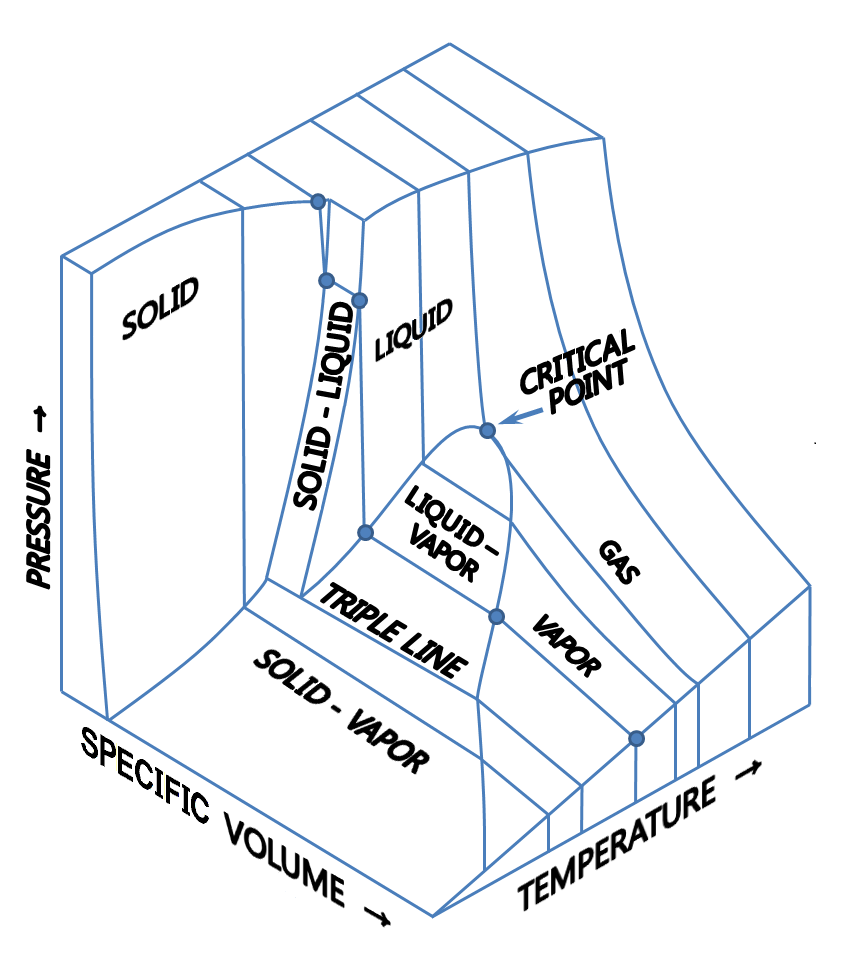
\includegraphics[width=0.5\linewidth]{./img/PVT_3D_diagram} 

}

\caption{The three-dimensional diagram.}\label{fig:FigTPVd}
\end{figure}

The critical point has coordinates \({T_c,P_c, \overline{V}_c}\). These critical coordinates can be determined from the vdW equation at \(T_c\), as:

\begin{equation}
T_c=\frac{8a}{27Rb} \qquad P_c=\frac{a}{27b^2} \qquad \overline{V}_c=3b, 
\label{eq:criticpt}
\end{equation}

These relations are used, in practice, to determine the vdW constants \(a,b\) from the experimentally measured critical isotherms.

The critical compressibility factor, \(z_c\), is predicted from the vdW equation at:

\begin{equation}
z_c=\frac{P_c \overline{V}_c}{R T_c}=\left( \frac{a}{27b^2} \right) \left( \frac{3b}{R} \right) \left( \frac{27Rb}{8a} \right) = \frac{3}{8} = 0.375,
\label{eq:critiz}
\end{equation}

a value that is independent of the gas. Experimentally measured values of \(z_c\) for different non-ideal gases are in the range of 0.2--0.3. These values can be used to infer the accuracy of the vdW equation for each non-ideal gas. Since the experimental \(z_c\) is usually lower than the one calculated from the vdW equation, we can deduce that the vdW equation overestimates the critical molar volume.

Notice how slicing the \(PT\overline{V}\) diagram at constant \(T\) results in the \(PV\) diagram that we reported in Figure \ref{fig:FigTPVd}. On the other hand, slicing the \(PT\overline{V}\) diagram at constant \(P\) results in the \(PT\) diagram that we will examine in detail in the next chapter.

\hypertarget{fugacity}{%
\section{Fugacity}\label{fugacity}}

The chemical potential of a pure ideal gas can be calculated using eq. \eqref{eq:dgconstn4}. Since we are not interested in mixture, we can drop the asterisk in \(\mu^*\), and rewrite eq. \eqref{eq:dgconstn4} as:

\begin{equation}
\mu_{\text{ideal}} = \mu^{-\kern-6pt{\ominus}\kern-6pt-}+ RT \ln \frac{P}{P^{-\kern-6pt{\ominus}\kern-6pt-}}.
\label{eq:dcpig}
\end{equation}

For a non-ideal gas, the pressure cannot be used in eq. \eqref{eq:dcpig} because each gas response to changes in pressure is not universal. We can, however, define a new variable to replace the pressure in eq. \eqref{eq:dcpig} and call it fugacity (\(f\)).

\begin{quote}
\begin{definition}
\protect\hypertarget{def:fugacitydef}{}{\label{def:fugacitydef} }\emph{Fugacity:} The effective pressure of a non-ideal gas that corresponds to the pressure of an ideal gas with the same temperature and chemical potential of the non-ideal one.
\end{definition}

Eq. \eqref{eq:dcpig} then becomes:
\end{quote}

\begin{equation}
\mu_{\text{non-ideal}} = \mu^{-\kern-6pt{\ominus}\kern-6pt-}+ RT \ln \frac{f}{P^{-\kern-6pt{\ominus}\kern-6pt-}}.
\label{eq:dcpnig}
\end{equation}

Since the chemical potential of a gas \(\mu\) is equal to the standard chemical potential \(\mu^{-\kern-6pt{\ominus}\kern-6pt-}\) when \(P=P^{-\kern-6pt{\ominus}\kern-6pt-}\), it is easy to use eq. \eqref{eq:dcpnig} to demonstrate that:

\begin{equation}
\lim_{P\rightarrow 0} \frac{f}{P} = 1,
\label{eq:dcpnigL}
\end{equation}

in other words, any non-ideal gas will approach the ideal gas behavior as \(P\rightarrow 0\). This condition, in conjunction with the \(T\rightarrow \infty\) behavior obtained in the previous section, results in the following statement:

\begin{quote}
The highest chances for any gas to behave ideally happen at high temperature and low pressure.
\end{quote}

We can now return our attention to the definition of fugacity. Remembering that the chemical potential is the molar Gibbs free energy of a substance, we can write:

\begin{equation}
d \mu_{\text{ideal}} = \overline{V}_{\text{ideal}}dP,
\label{eq:dmufug1}
\end{equation}

and:

\begin{equation}
d \mu_{\text{non-ideal}} = \overline{V}_{\text{non-ideal}}dP,
\label{eq:dmufug2}
\end{equation}

Subtracting eq. \eqref{eq:dmufug1} from eq. \eqref{eq:dmufug2}, we obtain:

\begin{equation}
d \mu_{\text{non-ideal}}-d \mu_{\text{ideal}} = \left(\overline{V}_{\text{non-ideal}}-\overline{V}_{\text{ideal}} \right) dP,
\label{eq:dmufug3}
\end{equation}

which we can then integrate between \(0\) and \(P\):

\begin{equation}
\mu_{\text{non-ideal}}-\mu_{\text{ideal}} = \int_0^P \left(\overline{V}_{\text{non-ideal}}-\overline{V}_{\text{ideal}} \right) dP.
\label{eq:dmufug4}
\end{equation}

Using eqs. \eqref{eq:dcpig} and \eqref{eq:dcpnig} we can then replace the definition of chemical potentials, resulting into:

\begin{equation}
\ln f - \ln P = \frac{1}{RT} \int_0^P \left(\overline{V}_{\text{non-ideal}} - \overline{V}_{\text{ideal}} \right) dP,
\label{eq:dmufug5}
\end{equation}

which gives us a mathematical definition of the fugacity, as:

\begin{equation}
f = P \cdot \underbrace{\exp\left[ \frac{1}{RT} \int_0^P \left(\overline{V}_{\text{non-ideal}}-\overline{V}_{\text{ideal}} \right) dP \right]}_{\text{fugacity coefficient, }\phi(T,P)}.
\label{eq:dmufug6}
\end{equation}

The exponential term in eq. \eqref{eq:dmufug6} is complicated to write, but it can be interpreted as a coefficient---unique to each non-ideal gas---that can be measured experimentally. Such coefficients are dependent on pressure and temperature and are called the \emph{fugacity coefficients}. Using letter \(\phi\) to represent the fugacity coefficient, we can rewrite eq. \eqref{eq:dmufug6} as:

\begin{equation}
f = \phi P,
\label{eq:dmufug7}
\end{equation}

which gives us a straightforward interpretation of the fugacity as an effective pressure. As such, the fugacity will have the same unit as the pressure, while the fugacity coefficients will be adimensional.

As we already saw in chapter \ref{ChemicalEquilibrium}, the fugacity can be used to replace the pressure in the definition of the equilibrium constant for reactions that involve non-ideal gases. The new constant is usually called \(K_f\), and is obtained from:

\begin{equation}
K_f=\prod_i f_{i,\text{eq}}^{\nu_i} = K_P \prod_i \phi_{i}^{\nu_i}.
\label{eq:kfdef}
\end{equation}

\renewcommand*{\standardstate}{{-\kern-6pt{\ominus}\kern-6pt-}}

\hypertarget{PhaseEquilibrium}{%
\chapter{Phase Equilibrium}\label{PhaseEquilibrium}}

\hypertarget{phase-stability}{%
\section{Phase Stability}\label{phase-stability}}

We have already encountered the gas, liquid, and solid phases and already discussed some of their properties. These terms are intuitive since these are the three most common states of matter.\footnote{Other states of matter---such as plasma---are possible, but they are not usually observed at the values of temperature and pressure that classical thermodynamics is usually applied to. Discussion of these extreme cases is beyond the scope of this textbook.} For this reason, we have previously used the terms without the necessity of formally defining their meaning. However, a formal definition of ``phase'' is necessary to discuss several concepts in this chapter and the following ones:

\begin{quote}
\begin{definition}
\protect\hypertarget{def:phasedef}{}{\label{def:phasedef} }\emph{Phase:} A region of the system with homogeneous chemical composition and physical state.
\end{definition}
\end{quote}

Let's now use the total differential of the chemical potential and the definition of molar Gibbs free energy for one component:

\begin{equation}
\begin{aligned}
d\mu &= \left( \frac{\partial \mu}{\partial T} \right)_P dT + \left( \frac{\partial \mu}{\partial P} \right)_T dP \\
d\mu &= -SdT+\overline{V}dP,
\end{aligned}
\label{eq:muequal1}
\end{equation}

to write:

\begin{equation}
\left( \frac{\partial \mu}{\partial T} \right)_P=-S \qquad \left( \frac{\partial \mu}{\partial P} \right)_T =\overline{V}.
\label{eq:muequal2}
\end{equation}

We can use these definitions to study the dependence of the chemical potential with respect to changes in pressure and temperature. If we plot \(\mu\) as a function of \(T\) using the first coefficient in eq. \eqref{eq:muequal2}, we obtain the diagram in Figure \ref{fig:FigPhase1}. The diagram presents three curves, each corresponding to one of the three most common states of matter -- solid, liquid, and gas. As we saw in several previous chapters, the entropy of a phase is almost constant with respect to temperature,\footnote{Think, for example, at the integral \(\int SdT\), for which we can assume \(S\) independent of temperature to obtain \(S\Delta T\). In practice, the entropy increases slightly with the temperature. Therefore the curves in Figure \ref{fig:FigPhase1} are slightly concave downwards (remember that they are obtained from values of \(-S\), so if \(S\) increase with \(T\), the curves bend downwards.)} and therefore the three curves are essentially straight, with negative angular coefficients \(-S\). This also explains why the solid phase has a basically flat line since, according to the third law, the entropy of a perfect solid is zero and close to zero if the solid is not perfect. The difference between the three lines' angular coefficients is explained by the fact that each of these states has a different value of entropy:

\begin{equation}
\left( \frac{\partial \mu_{\text{solid}}}{\partial T} \right)_P =-S_{\text{s}} \qquad \left( \frac{\partial \mu_{\text{liquid}}}{\partial T} \right)_P =-S_{\text{l}} \qquad \left( \frac{\partial \mu_{\text{gas}}}{\partial T} \right)_P =-S_{\text{g}},
\label{eq:muequal3}
\end{equation}

and since the entropy of a gas is always bigger than the entropy of a liquid, which in turn, is yet bigger than the entropy of a solid (\(S_{\text{g}} \gg S_{\text{l}}>S_{\text{s}}\)), we obtain three lines with different angular coefficients that intersect each other. At each temperature, the phase with the lowest chemical potential will be the most stable (see red segments in Figure \ref{fig:FigPhase1}). At each intersection between two lines, the two phases have the same chemical potential, representing the temperature at which they coexist. This temperature is the temperature at which the phase change happens. Recalling from general chemistry, at the junction between the solid and the liquid lines, the fusion (fus) process occurs, and the corresponding temperature is called the melting point \(T_{\text{m}}\). At the junction between the liquid and the gas lines, the vaporization (vap) process happens, and the corresponding temperature is called the boiling point \(T_{\text{b}}\). Depending on the substance and the pressure at which the process happens, the solid line might intersect the gas line before the liquid line. When that occurs, the liquid phase is never observed, and only the sublimation (subl) process happens at the sublimation point \(T_{\text{subl}}\).

\begin{figure}

{\centering 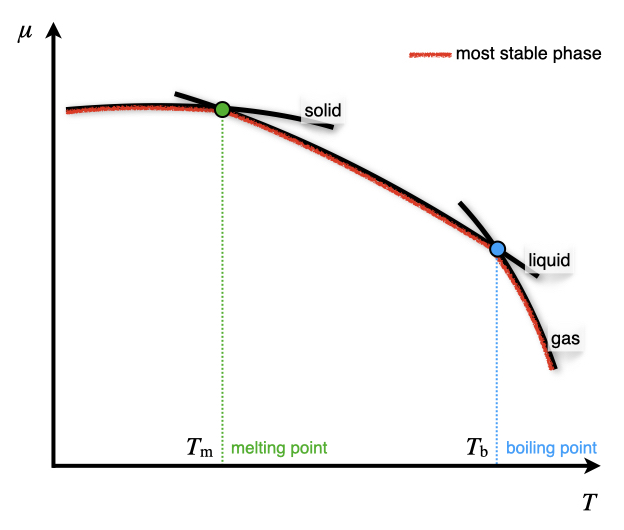
\includegraphics[width=0.6\linewidth]{./img/OEP_Figures.016} 

}

\caption{Dependence of the Chemical Potentials of Solid, Liquid, and Gas Phases on Temperature at Constant Pressure.}\label{fig:FigPhase1}
\end{figure}

The effects of pressure on this diagram can be studied using the second coefficient in eq. \eqref{eq:muequal2}. For the majority of substances, \(\overline{V}_{\text{g}} \gg \overline{V}_{\text{l}} > \overline{V}_{\text{s}}\), hence the curves will shift to lower values when the pressure is reduced, as in Figure \ref{fig:FigPhase2}. Notice also that since \(\overline{V}_{\text{l}} \cong \overline{V}_{\text{s}}\), the shifts for both the solid and liquid lines is much smaller than the shift for the gas line. These shifts also translate to different values of the junctions, which means the phase changes will occur at different temperatures. Therefore both the melting point and the boiling point in general decrease when pressure is increased (and vice versa). Notice how the change for the melting point is always much smaller than the change for the boiling point.
Water is a noticeable exception to these trend because \(\overline{V}_{\mathrm{H}_2\mathrm{O,l}} < \overline{V}_{\text{ice}}\). This explains the experimental observation that increasing the pressure on ice causes the ice to melt\footnote{Despite the effect being minimal, it is one of the contributing causes to the fact that we can skate on ice, but we can't on stone. If we increase our pressure on ice by reducing our footprints' surface area using thin skates, ice will slightly melt under our own weight, creating a thin liquid film on which we can skate because of the reduced friction.}

\begin{figure}

{\centering 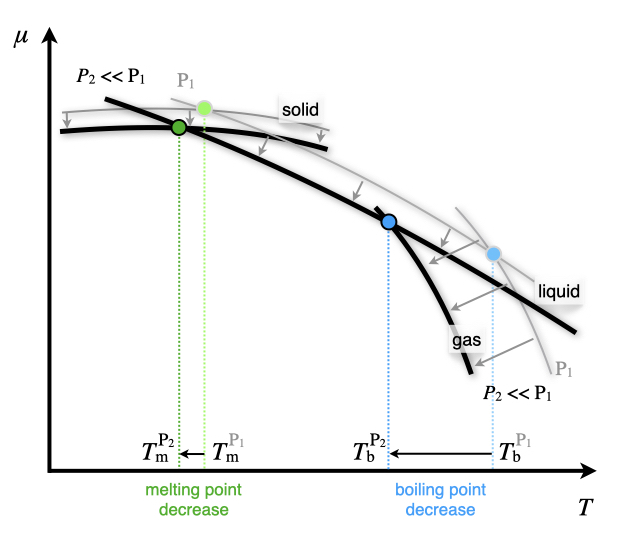
\includegraphics[width=0.6\linewidth]{./img/OEP_Figures.017} 

}

\caption{Effect of Pressure on the Chemical Potential Diagram.}\label{fig:FigPhase2}
\end{figure}

Considering the intersections between two lines, two phases are in equilibrium with each other at each of these points. Therefore their chemical potentials must be equal:

For two or more phases to be in equilibrium, their chemical potential must be equal:

\begin{equation}
\mu_{\alpha} = \mu_{\beta}.
\label{eq:muequal}
\end{equation}

If we now change either the temperature or the pressure, the location of the intersection will be shifted (see again Figure \ref{fig:FigPhase2} and the discussion above). For infinitesimal changes in variables, the new location will be:

\begin{equation}
\mu_{\alpha} + d\mu_{\alpha}= \mu_{\beta}+d\mu_{\beta},
\label{eq:muequalA}
\end{equation}

which using eq. \eqref{eq:muequal}, simply becomes:

\begin{equation}
d\mu_{\alpha}= d\mu_{\beta}.
\label{eq:muequalB}
\end{equation}

Replacing the differential with the definition of chemical potential in eq. \eqref{eq:muequal1}, we obtain:

\begin{equation}
\begin{aligned}
-S_{\alpha}dT+\overline{V}_{\alpha} &= -S_{\beta}dT+\overline{V}_{\beta} \\
\underbrace{\left(S_{\beta}-S_{\alpha}\right)}_{\Delta S} dT &= \underbrace{\left( \overline{V}_{\beta}-\overline{V}_{\alpha}\right)}_{\Delta \overline{V}},
\end{aligned}
\label{eq:muequalC}
\end{equation}

which can be rearranged into:

\begin{equation}
\frac{dP}{dT}=\frac{\Delta S}{\Delta \overline{V}}.
\label{eq:ClapeyronEq}
\end{equation}

This equation is known as the \textbf{Clapeyron equation}, and it is the mathematical relation at the basis of the pressure-temperature phase diagrams. Plotting the results of eq. \eqref{eq:ClapeyronEq} on a \(PT\) phase diagram for common substances results in three lines representing the equilibrium between two different phases. These diagrams are useful to study the relationship between the phases of a substance.

\hypertarget{gibbs-phase-rule}{%
\section{Gibbs Phase Rule}\label{gibbs-phase-rule}}

In chapter \ref{SystemVariables}, we have already seen that the number of independent variables required to describe an ideal gas is two. This number was derived by counting the total number of variables \((3: P,\overline{V},T)\), and reduce it by one because the ideal gas law constrains the value of one of them, once the other two are fixed. For a generic system potentially containing more than one chemical substance in several different phases, however, the number of independent variables can be different than two. For a system composed of \(c\) components (chemical substances) and \(p\) phases, the number of independent variables, \(f\), is given by the Gibbs phase rule:

\begin{equation}
f=c-p+2.
\label{eq:Gibbsrule}
\end{equation}

The Gibbs phase rule derives from the fact that different phases are in equilibrium with each other at some conditions, resulting in the reduction of the number of independent variables at those conditions. More rigorously, when two phases are in thermodynamic equilibrium, their chemical potentials are equal (see eq. \eqref{eq:muequal}). For each equality, the number of independent variables---also called the number of \emph{degrees of freedom}---is reduced by one. For example, the chemical potentials of the liquid and its vapor depend on both \(T\) and \(P\). But when these phases are in equilibrium with each other, their chemical potentials must be equal. If either the pressure or the temperature is fixed, the other variable will be uniquely determined by the equality relation. In other terms, when a liquid is in equilibrium with its vapor at a given pressure, the temperature is determined by the fact that the chemical potentials of the two phases is the same, and is denoted as the boiling temperature \(T_{\text{b}}\). Similarly, at a given temperature, the pressure of the vapor is uniquely determined by the same equality relation and is denoted as the vapor pressure, \(P^*\).

The Gibbs phase rule is obtained considering that the number of independent variables is given by the total number of variables minus the constraints. The total number of variables is given by temperature, pressure, plus all the variables required to describe each of the phases. The composition of each phase is determined by \((c-1)\) variables.\footnote{For a 1-component system \(c-1=1-1=0\), and no additional variable is required to determine the composition of each phase. For a 2-component system, however, each phase will contain both components, hence \(c-1=2-1=1\) additional variable will be required to describe it--the mole fraction.} The number of constraints is determined by the number of possible equilibrium relations, which is \(c(p-1)\) since the chemical potential of each component must be equal in all phases. The number of degrees of freedom \(f\) is then given by \(f=(c-1)p+2-c(p-1)\) \(=c-p+2\), which is the Gibbs phase rule, as in eq. \eqref{eq:Gibbsrule}.

\hypertarget{pt-phase-diagrams}{%
\section{\texorpdfstring{\(PT\) Phase Diagrams}{PT Phase Diagrams}}\label{pt-phase-diagrams}}

\begin{figure}

{\centering 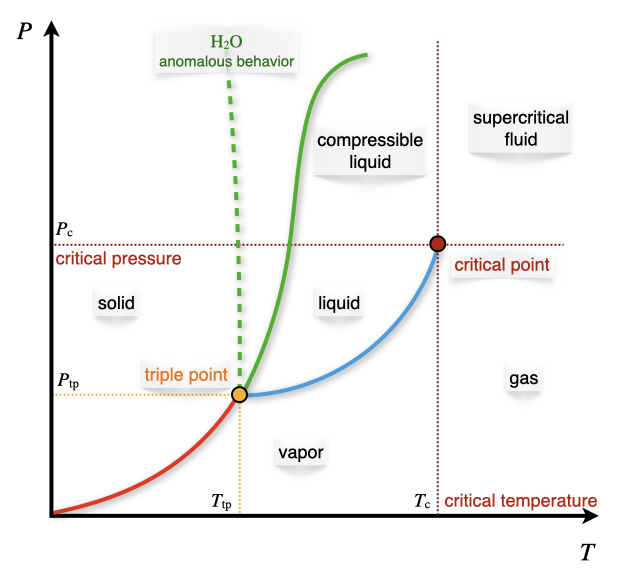
\includegraphics[width=0.6\linewidth]{./img/OEP_Figures.018} 

}

\caption{The Pressure–Temperature Phase Diagram.}\label{fig:FigPhase3}
\end{figure}

Let's now discuss the pressure--temperature diagram of a typical substance, as reported in Figure \ref{fig:FigPhase3}. Each of the lines reported in the diagram represents an equilibrium between two phases, and therefore it represents a condition that reduces the number of degrees of freedom to one. The lines can be determined using the Clapeyron equation, eq. \eqref{eq:ClapeyronEq}. The interpretation of each line is as follows:

\hypertarget{liquid-rightleftarrows-gas-equilibrium}{%
\subsection{\texorpdfstring{Liquid \(\rightleftarrows\) Gas equilibrium}{Liquid \textbackslash rightleftarrows Gas equilibrium}}\label{liquid-rightleftarrows-gas-equilibrium}}

For this equilibrium we can use Trouton's rule, eq. \eqref{eq:trouton}, and write:
\begin{equation}
\Delta_{\text{vap}} S = S_{\text{g}}-S_{\text{l}} \cong 88 \; \frac{\text{kJ}}{\text{mol}} > 0\quad \text{always},
\label{eq:PTdia1}
\end{equation}

where the entropy of vaporization is always positive, even for cases where the Trouton's rule is violated. The difference in molar volumes is easily obtained, since the volume of the gas is always much greater than the volume of the liquid:

\begin{equation}
\overline{V}_{\text{g}} - \overline{V}_{\text{l}} \cong \overline{V}_{\text{g}} = 22.4\; \frac{\text{L}}{\text{mol}} >0\quad \text{always}.
\label{eq:PTdia2}
\end{equation}

Replacing these values in the Clapeyron equation, we obtain:

\begin{equation}
\frac{dP}{dT}=\frac{88}{22.4}\left( \frac{0.0831}{8.31} \right) = 0.004\;\text{bar} > 0 \quad \text{always},
\label{eq:PTdia3}
\end{equation}

which is always positive,regardless of violations to the Trouton's rule. Notice how small this value is, meaning that the liquid--gas equilibrium curve is mostly flat as \(T\rightarrow 0\).

\hypertarget{solid-rightleftarrows-gas-equilibrium}{%
\subsection{\texorpdfstring{Solid \(\rightleftarrows\) Gas equilibrium}{Solid \textbackslash rightleftarrows Gas equilibrium}}\label{solid-rightleftarrows-gas-equilibrium}}

If we look at the signs of each quantity, this case is similar to the previous one:
\begin{equation}
\begin{aligned}
\Delta_{\text{subl}} S &> 0 \quad \text{always} \\
\Delta_{\text{subl}} \overline{V }&> 0 \quad \text{always} \\
\\
\frac{dP}{dT} &> 0 \quad \text{always}.
\end{aligned}
\label{eq:PTdi1}
\end{equation}

However, the Trouton's rule is not valid for the solid--gas equilibrium, and \(\frac{dP}{dT}\) will be larger than for the previous case.

\hypertarget{solid-rightleftarrows-liquid-equilibrium}{%
\subsection{\texorpdfstring{Solid \(\rightleftarrows\) Liquid equilibrium}{Solid \textbackslash rightleftarrows Liquid equilibrium}}\label{solid-rightleftarrows-liquid-equilibrium}}

The final curve is for the solid-liquid equilibrium, for which we have:

\begin{equation}
\Delta_{\text{fus}} S = \frac{\Delta_{\text{fusion}} H}{T_{\text{m}}} > 0 \quad \text{always},
\label{eq:PTd1}
\end{equation}

since fusion is always an exothermic process, \((\Delta_{\text{fus}} H>0)\). On the other side:

\begin{equation}
\Delta_{\text{fusion}} \overline{V} = \overline{V}_{\text{l}} - \overline{V}_{\text{s}} > 0 \quad \text{generally}.
\end{equation}

In other words, the difference of the molar volume of the liquid and that of the solid is positive for most substances, but it might be negative (for example for \(\mathrm{H}_2\mathrm{O}\)). As such:

\begin{equation}
 \frac{dP}{dT} > 0 \quad \text{generally}.
\label{eq:PTd2}
\end{equation}

For \(\mathrm{H}_2\mathrm{O}\) and a few other substances, \(\frac{dP}{dT}<0\), an anomalous behavior that has crucial consequences for the existence of life on earth.\footnote{As is well explained by \href{https://en.wikipedia.org/wiki/Properties_of_water\#Density_of_water_and_ice}{Wikipedia}: ``The unusual density curve and lower density of ice than of water is vital to life---if water were most dense at the freezing point, then in winter the very cold water at the surface of lakes and other water bodies would sink, lakes could freeze from the bottom up, and all life in them would be killed. Furthermore, given that water is a good thermal insulator (due to its heat capacity), some frozen lakes might not completely thaw in summer.{[}34{]} The layer of ice that floats on top insulates the water below. Water at about 4 °C (39 °F) also sinks to the bottom, thus keeping the temperature of the water at the bottom constant.''} For this importance, this behavior is also depicted in Figure \ref{fig:FigPhase3} using a dashed green line.

Since the differences in molar volumes between the solid and the liquid phases are usually small (changes are generally of the order of \(10^{-3}\;\mathrm{L}\)), \(\frac{dP}{dT}\) is always much larger than for the previous two cases. The resulting lines for the solid--liquid equilibria are still almost vertical, regardless of the signs of their angular coefficients.

\hypertarget{the-triple-point-and-the-critical-point}{%
\subsection{The triple point and the critical point}\label{the-triple-point-and-the-critical-point}}

The only point in the \(PT\) diagram where all the three phases coexist is called the triple point. The number of degrees of freedom at the triple point for every 1-component diagram is \(f=1-3+2=0\). The fact that the triple point has zero degrees of freedom means that its coordinates, \({T_{\text{tp}},P_{\text{tp}},\overline{V}_{\text{tp}}}\), are uniquely determined for each chemical substance. For this reason, the value of the triple point of water was fixed by definition---rather than measured---until 2019. This definition was necessary to establish the base unit of the thermodynamic temperature scale in the SI (the Kelvin).\footnote{For more information on the 2019 redefinition of the SI units, see \href{https://en.wikipedia.org/wiki/2019_redefinition_of_the_SI_base_units}{this Wikipedia page}.}

In addition to the triple point where the solid, liquid, and gas phases meet, a triple point may involve more than one condensed phase. Triple points are common for substances with multiple solid phases (polymorphs), involving either two solid phases and a liquid one or three solid phases. Helium is a special case that presents a triple point involving two different fluid phases, called the lambda point. Since the number of degrees of freedom cannot be negative, the Gibbs phase rule for a 1-component diagram sets the limit to how many phases can coexist to just three. Therefore, quadruple points (or higher coexistence points) are not possible for pure substances, even for polymorphs.\footnote{Notice that quadruple points are possible for 2-component diagrams.}

Another point with a fixed position in the \(PT\) diagram is the critical point, \({T_{\text{c}},P_{\text{c}},\overline{V}_{\text{c}}}\). We have already given the definition of the critical temperature in \ref{def:criticalT}. This point represents the end of the liquid--gas equilibrium curve. This point is also semantically important to define different regions of the phase diagram, as in Figure \ref{fig:FigPhase3}. A gas whose pressure and temperature are below the critical point is called a \emph{vapor}. A gas whose temperature and pressure are above the critical point is called a \emph{supercritical fluid}. Finally, a liquid whose pressure is above the critical point is called a \emph{compressible liquid}.\footnote{Notice that the temperature of a liquid must be below the critical point, otherwise it is no longer a liquid but rather a supercritical fluid.}

\hypertarget{the-clausiusclapeyron-equation}{%
\section{The Clausius--Clapeyron Equation}\label{the-clausiusclapeyron-equation}}

Let's now take a closer look at the equilibrium between a condensed phase and the gas phase. For both the vaporization and sublimation processes, Clausius showed that the Clapeyron equation can be simplified by using:

\begin{equation}
 \Delta_{\text{vap}} S = \frac{\Delta_{\text{vap}} H}{T} \qquad \Delta \overline{V}= \overline{V}_{\mathrm{g}} -\overline{V}_{\mathrm{l}} \cong \overline{V}_{\mathrm{g}},
\label{eq:clacla1}
\end{equation}

resulting in:

\begin{equation}
 \frac{dP}{dT} = \frac{ \Delta_{\text{vap}} S}{\Delta \overline{V}} \cong \frac{ \Delta_{\text{vap}} H}{T \overline{V}_{\mathrm{g}}}.
\label{eq:clacla2}
\end{equation}

Using the ideal gas law to replace the molar volume of the gas, we obtain:

\begin{equation}
 \frac{dP}{dT} = \frac{P \Delta_{\text{vap}} H}{RT^2},
\label{eq:clacla3}
\end{equation}

which can be rearranged as:

\begin{equation}
 \frac{dP}{P} = \frac{\Delta_{\text{vap}} H}{R} \frac{dT}{T^2}.
\label{eq:clacla}
\end{equation}

Eq. \eqref{eq:clacla} is known as the \textbf{Clausius--Clapeyron equation}, and it measures the dependence of the vapor pressure of a substance as a function of the temperature. The Clausius--Clapeyron equation can be integrated to obtain:

\begin{equation}
\begin{aligned}
\int_{P_i}^{P_f} \frac{dP}{P} &= \frac{\Delta_{\text{vap}} H}{R} \int_{T_i}^{T_f} \frac{dT}{T^2} \\
\ln \frac{P_f}{P_i} &=-\frac{\Delta_{\text{vap}} H}{R} \left( \frac{1}{T_f}-\frac{1}{T_i} \right).
\end{aligned}
\label{eq:clacla4}
\end{equation}

The integrated Clausius--Clapeyron equation shows that the vapor pressure depends exponentially on the temperature. Thus, even a small change in the temperature will result in a significant change in the vapor pressure. In fact, we daily use the fact that the vapor pressure of water changes drastically when we increase its temperature for cooking most of our food. For example, at an external pressure of 1 bar, it rapidly grows from \(P^*=0.02\;\text{bar}\) to \(P^*=1\;\text{bar}\) when the temperature is increased from \(T=293\;\mathrm{K}\) (around room temperature) to \(T=373\;\mathrm{K}\) (boiling point). The integrated Clausius--Clapeyron equation is also often used to determine the enthalpy of vaporization from measurements of vapor pressure at different temperatures.

\hypertarget{MCPhaseDiagrams}{%
\chapter{Multi-Component Phase Diagrams}\label{MCPhaseDiagrams}}

We now move from studying 1-component systems to multi-component ones. Systems that include two or more chemical species are usually called \emph{solutions}. Solutions are possible for all three states of matter:

\scriptsize

\begin{longtable}[]{@{}lccl@{}}
\toprule
Type: & Solvent & Solute & Examples:\tabularnewline
\midrule
\endhead
Solid solutions & Solid & Solid & Alloys: brass, bronze\tabularnewline
& Solid & Liquid & Dental amalgam\tabularnewline
& Solid & Gas & Hydrogen stored in Palladium\tabularnewline
Liquid solutions & Liquid & Solid & Saltwater, bleach\tabularnewline
& Liquid & Liquid & Alcoholic beverages, vinegar\tabularnewline
& Liquid & Gas & Carbonated drinks\tabularnewline
Gaseous solutions & Gas & Solid & Smoke, smog\tabularnewline
& Gas & Liquid & Aerosols and perfumes\tabularnewline
& Gas & Gas & Air\tabularnewline
\bottomrule
\end{longtable}

\normalsize

The number of degrees of freedom for binary solutions (solutions containing two components) is calculated from the Gibbs phase rules at \(f=2-p+2=4-p\). When one phase is present, binary solutions require \(4-1=3\) variables to be described, usually temperature (\(T\)), pressure (\(P\)), and mole fraction (\(y_i\) in the gas phase and \(x_i\) in the liquid phase). Single-phase, 1-component systems require three-dimensional \(T,P,x_i\) diagram to be described. When two phases are present (e.g., gas and liquid), only two variables are independent: pressure and concentration. Thus, we can study the behavior of the partial pressure of a gas--liquid solution in a 2-dimensional plot. If the gas phase in a solution exhibits properties similar to those of a mixture of ideal gases, it is called an \emph{ideal solution}. The obvious difference between ideal solutions and ideal gases is that the intermolecular interactions in the liquid phase cannot be neglected as for the gas phase. The main advantage of ideal solutions is that the interactions between particles in the liquid phase have similar mean strength throughout the entire phase. We will consider ideal solutions first, and then we'll discuss deviation from ideal behavior and non-ideal solutions.

\hypertarget{raoults-law-and-phase-diagrams-of-ideal-solutions}{%
\section{Raoult's Law and Phase Diagrams of Ideal Solutions}\label{raoults-law-and-phase-diagrams-of-ideal-solutions}}

The behavior of the vapor pressure of an ideal solution can be mathematically described by a simple law established by François-Marie Raoult (1830--1901). \textbf{Raoult's law} states that the partial pressure of each component, \(i\), of an ideal mixture of liquids, \(P_i\), is equal to the vapor pressure of the pure component \(P_i^*\) multiplied by its mole fraction in the mixture \(x_i\):

\begin{equation}
P_i=x_i P_i^*.
\label{eq:mc1}
\end{equation}

\hypertarget{one-volatile-component}{%
\subsection{One volatile component}\label{one-volatile-component}}

Raoult's law applied to a system containing only one volatile component describes a line in the \(Px_{\text{B}}\) plot, as in Figure \ref{fig:FigMC1}.

\begin{figure}

{\centering 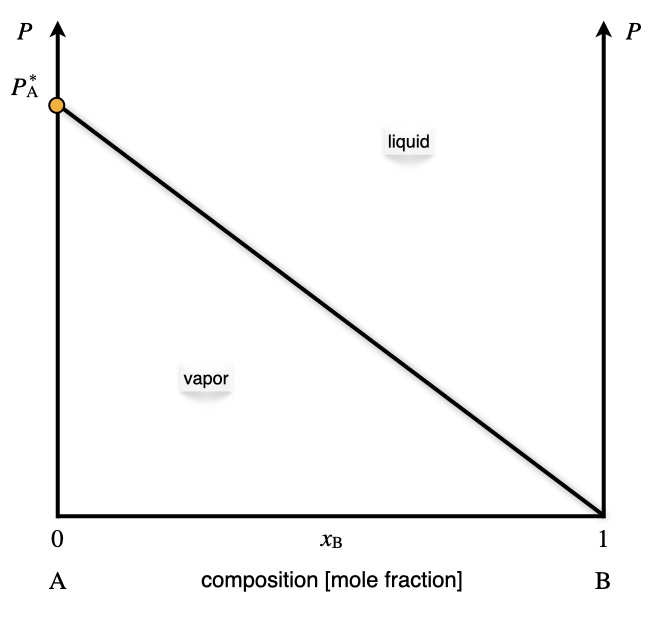
\includegraphics[width=0.6\linewidth]{./img/OEP_Figures.019} 

}

\caption{The Pressure–Composition Phase Diagram of an Ideal Solution Containing a Single Volatile Component at Constant Temperature.}\label{fig:FigMC1}
\end{figure}

As emerges from Figure \ref{fig:FigMC1}, Raoult's law divides the diagram into two distinct areas, each with three degrees of freedom.\footnote{Only two degrees of freedom are visible in the \(Px_{\text{B}}\) diagram. Temperature represents the third independent variable.} Each area contains a phase, with the vapor at the bottom (low pressure), and the liquid at the top (high pressure). Raoult's law acts as an additional constraint for the points sitting on the line. Therefore, the number of independent variables along the line is only two. Once the temperature is fixed, and the vapor pressure is measured, the mole fraction of the volatile component in the liquid phase is determined.

\hypertarget{two-volatile-components}{%
\subsection{Two volatile components}\label{two-volatile-components}}

In an ideal solution, every volatile component follows Raoult's law. Since the vapors in the gas phase behave ideally, the total pressure can be simply calculated using Dalton's law as the sum of the partial pressures of the two components \(P_{\text{TOT}}=P_{\text{A}}+P_{\text{B}}\). The corresponding diagram is reported in Figure \ref{fig:FigMC2}. The total vapor pressure, calculated using Dalton's law, is reported in red. The Raoult's behaviors of each of the two components are also reported using black dashed lines.

\begin{figure}

{\centering 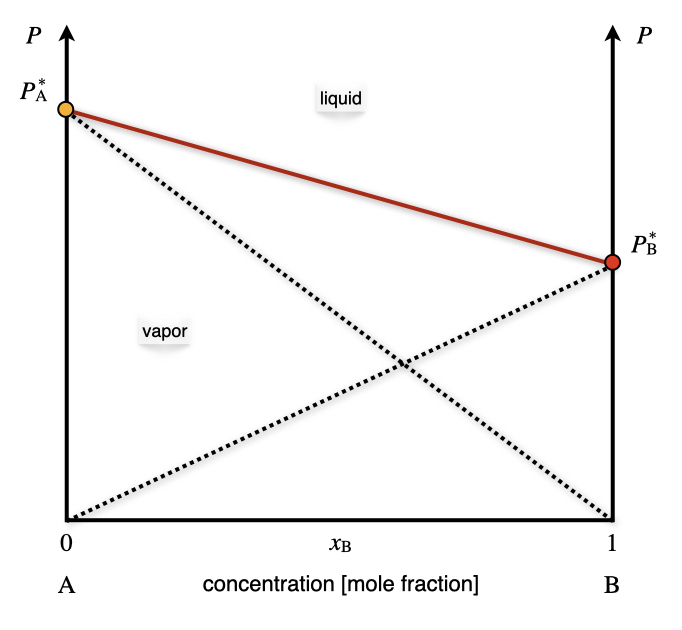
\includegraphics[width=0.6\linewidth]{./img/OEP_Figures.020} 

}

\caption{The Pressure–Composition Phase Diagram of an Ideal Solution Containing Two Volatile Components at Constant Temperature.}\label{fig:FigMC2}
\end{figure}

\begin{quote}
\begin{exercise}
\protect\hypertarget{exr:xaya}{}{\label{exr:xaya} }Calculate the mole fraction in the vapor phase of a liquid solution composed of 67\% of toluene (\(\mathrm{A}\)) and 33\% of benzene (\(\mathrm{B}\)), given the vapor pressures of the pure substances: \(P_{\text{A}}^*=0.03\;\text{bar}\), and \(P_{\text{B}}^*=0.10\;\text{bar}\).
\emph{Solution:} The data available for the systems are summarized as follwos:
\begin{equation}
\begin{aligned}
x_{\text{A}}=0.67  \qquad & \qquad x_{\text{B}}=0.33 \\
P_{\text{A}}^* = 0.03\;\text{bar} \qquad & \qquad P_{\text{B}}^* = 0.10\;\text{bar} \\
& P_{\text{TOT}}^* = ? \\
y_{\text{A}}=? \qquad & \qquad y_{\text{B}}=?
\end{aligned}
\label{eq:mc2}
\end{equation}
The total pressure of the vapors can be calculated combining Dalton's and Roult's laws:
\begin{equation}
\begin{aligned}
P_{\text{TOT}} &= P_{\text{A}}+P_{\text{B}}=x_{\text{A}} P_{\text{A}}^* + x_{\text{B}} P_{\text{B}}^* \\
&= 0.67\cdot 0.03+0.33\cdot 0.10 \\
&= 0.02 + 0.03 = 0.05 \;\text{bar}
\end{aligned}
\label{eq:mc3}
\end{equation}
We can then calculate the mole fraction of the components in the vapor phase as:
\begin{equation}
\begin{aligned}
y_{\text{A}}=\frac{P_{\text{A}}}{P_{\text{TOT}}} & \qquad y_{\text{B}}=\frac{P_{\text{B}}}{P_{\text{TOT}}} \\
y_{\text{A}}=\frac{0.02}{0.05}=0.40 & \qquad y_{\text{B}}=\frac{0.03}{0.05}=0.60
\end{aligned}
\label{eq:mc4}
\end{equation}
Notice how the mole fraction of toluene is m uch higher in the liquid phase, \(x_{\text{A}}=0.67\), than in the vapor phase, \(y_{\text{A}}=0.40\).
\end{exercise}
\end{quote}

As is clear from the results of Exercise \ref{exr:xaya}, the concentration of the components in the gas and vapor phases are different. We can also report the mole fraction in the vapor phase as an additional line in the \(Px_{\text{B}}\) diagram of Figure \ref{fig:FigMC2}. When both concentrations are reported in one diagram---as in Figure \ref{fig:FigMC3}---the line where \(x_{\text{B}}\) is obtained is called the \emph{liquidus line}, while the line where the \(y_{\text{B}}\) is reported is called the \emph{Dew point line}.

\begin{figure}

{\centering 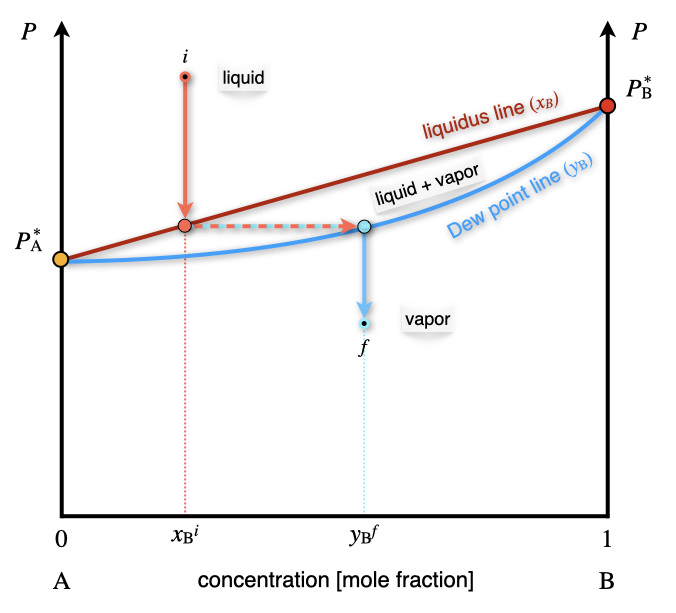
\includegraphics[width=0.6\linewidth]{./img/OEP_Figures.021} 

}

\caption{The Pressure–Composition Phase Diagram of an Ideal Solution Containing Two Volatile Components at Constant Temperature. Both the Liquidus and Dew Point Line are Emphasized in this Plot.}\label{fig:FigMC3}
\end{figure}

The liquidus and Dew point lines determine a new section in the phase diagram where the liquid and vapor phases coexist. Since the degrees of freedom inside the area are only 2, for a system at constant temperature, a point inside the coexistence area has fixed mole fractions for both phases. We can reduce the pressure on top of a liquid solution with concentration \(x^i_{\text{B}}\) (see Figure \ref{fig:FigMC3}) until the solution hits the liquidus line. At this pressure, the solution forms a vapor phase with mole fraction given by the corresponding point on the Dew point line, \(y^f_{\text{B}}\).

\hypertarget{t_textb-phase-diagrams-and-fractional-distillation}{%
\subsection{\texorpdfstring{\(T_{\text{B}}\) phase diagrams and fractional distillation}{T\_\{\textbackslash text\{B\}\} phase diagrams and fractional distillation}}\label{t_textb-phase-diagrams-and-fractional-distillation}}

We can now consider the phase diagram of a 2-component ideal solution as a function of temperature at constant pressure. The \(T_{\text{B}}\) diagram for two volatile components is reported in Figure \ref{fig:FigMC4}.

\begin{figure}

{\centering 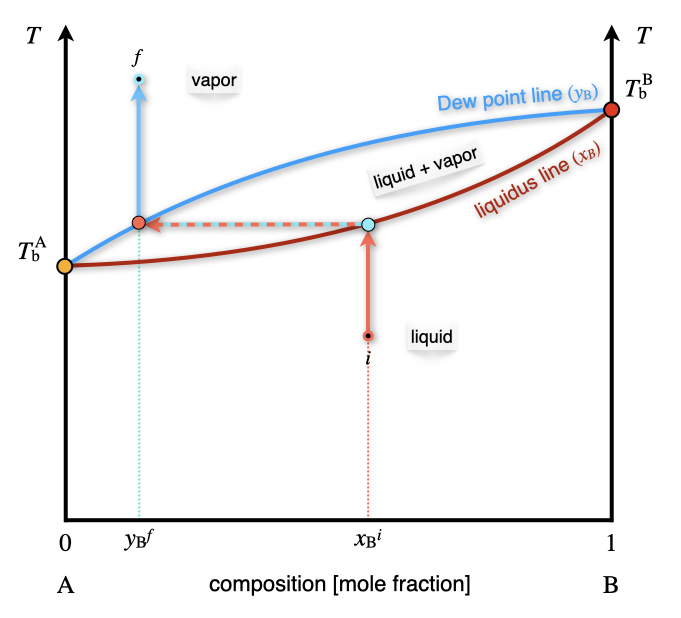
\includegraphics[width=0.6\linewidth]{./img/OEP_Figures.022} 

}

\caption{The Temperature–Composition Phase Diagram of an Ideal Solution Containing Two Volatile Components at Constant Pressure.}\label{fig:FigMC4}
\end{figure}

Compared to the \(Px_{\text{B}}\) diagram of Figure \ref{fig:FigMC3}, the phases are now in reversed order, with the liquid at the bottom (low temperature), and the vapor on top (high Temperature). The liquidus and Dew point lines are curved and form a lens-shaped region where liquid and vapor coexists. Once again, there is only one degree of freedom inside the lens. As such, a liquid solution of initial composition \(x_{\text{B}}^i\) can be heated until it hits the liquidus line. At this temperature the solution boils, producing a vapor with concentration \(y_{\text{B}}^f\). As is clear from Figure \ref{fig:FigMC4}, the mole fraction of the \(\text{B}\) component in the gas phase is lower than the mole fraction in the liquid phase. This fact can be exploited to separate the two components of the solution. In particular, if we set up a series of consecutive evaporation and condensations, we can distill fractions of the solution with an increasingly lower concentration of the less volatile component \(\text{B}\). This is exemplified in the industrial process of fractional distillation, as schematically depicted in Figure \ref{fig:FigMC5}.

\begin{figure}

{\centering 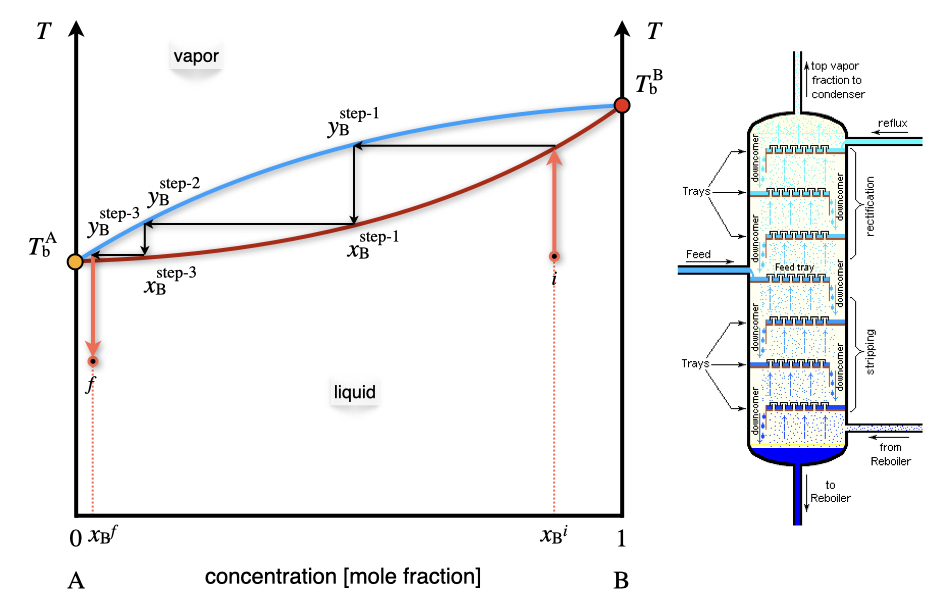
\includegraphics[width=0.6\linewidth]{./img/OEP_Figures.023} 

}

\caption{The Fractional Distillation Process and Theoretical Plates Calculated on a Temperature–Composition Phase Diagram.}\label{fig:FigMC5}
\end{figure}

Each of the horizontal lines in the lens region of the \(Tx_{\text{B}}\) diagram of Figure \ref{fig:FigMC5} corresponds to a condensation/evaporation process and is called a \emph{theoretical plate}. These plates are industrially realized on large columns with several floors equipped with condensation trays. The temperature decreases with the height of the column. A condensation/evaporation process will happen on each level, and a solution concentrated in the most volatile component is collected. The theoretical plates and the \(Tx_{\text{B}}\) are crucial for sizing the industrial fractional distillation columns.

\hypertarget{phase-diagrams-of-non-ideal-solutions}{%
\section{Phase Diagrams of Non-Ideal Solutions}\label{phase-diagrams-of-non-ideal-solutions}}

Non-ideal solutions follow Raoult's law for only a small amount of concentrations. The typical behavior of a non-ideal solution with a single volatile component is reported in the \(Px_{\text{B}}\) plot in Figure \ref{fig:FigMC6}.

\begin{figure}

{\centering 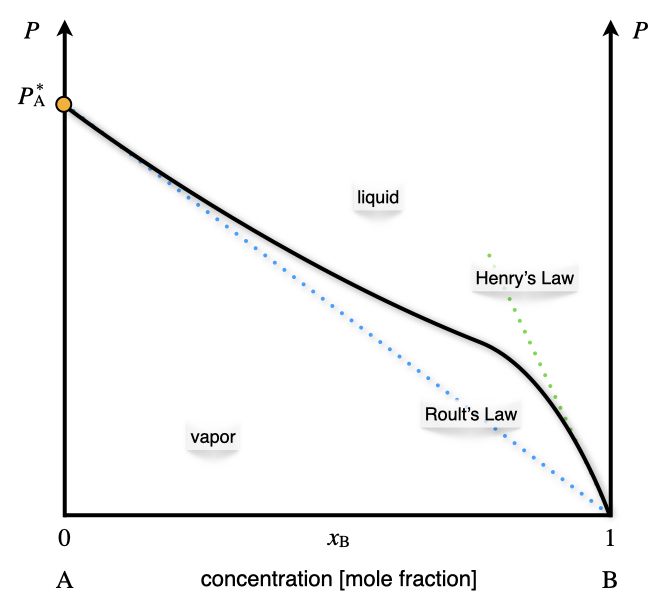
\includegraphics[width=0.6\linewidth]{./img/OEP_Figures.024} 

}

\caption{The Pressure–Composition Phase Diagram of a Non-Ideal Solution Containing a Single Volatile Component at Constant Temperature.}\label{fig:FigMC6}
\end{figure}

Raoult's behavior is observed for high concentrations of the volatile component. This behavior is observed at \(x_{\text{B}} \rightarrow 0\) in Figure \ref{fig:FigMC6}, since the volatile component in this diagram is \(\mathrm{A}\). At low concentrations of the volatile component \(x_{\text{B}} \rightarrow 1\) in Figure \ref{fig:FigMC6}, the solution follows a behavior along a steeper line, which is known as \textbf{Henry's law}. William Henry (1774--1836) has extensively studied the behavior of gases dissolved in liquids. His studies resulted in a simple law that relates the vapor pressure of a solution to a constant, called Henry's law solubility constants:

\begin{equation}
P_{\text{B}}=k_{\text{AB}} x_{\text{B}},
\label{eq:mc1b}
\end{equation}

where \(k_{\text{AB}}\) depends on the chemical nature of \(\mathrm{A}\) and \(\mathrm{B}\). The corresponding diagram for non-ideal solutions with two volatile components is reported on the left panel of Figure \ref{fig:FigMC7}. The total pressure is once again calculated as the sum of the two partial pressures. Positive deviations on Raoult's ideal behavior are not the only possible deviation from ideality, and negative deviation also exits, albeit slightly less common. An example of a negative deviation is reported in the right panel of Figure \ref{fig:FigMC7}.

\begin{figure}

{\centering 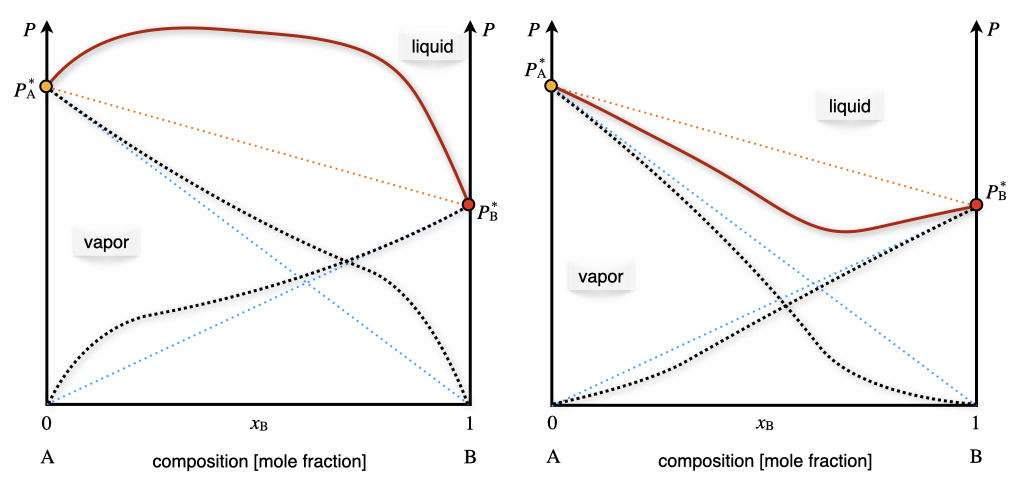
\includegraphics[width=0.8\linewidth]{./img/OEP_Figures.025} 

}

\caption{The Pressure–Composition Phase Diagram of Non-Ideal Solutions Containing Two Volatile Components at Constant Temperature.}\label{fig:FigMC7}
\end{figure}

If we move from the \(Px_{\text{B}}\) diagram to the \(Tx_{\text{B}}\) diagram, the behaviors observed in Figure \ref{fig:FigMC7} will correspond to the diagram in Figure \ref{fig:FigMC8}.

\begin{figure}

{\centering 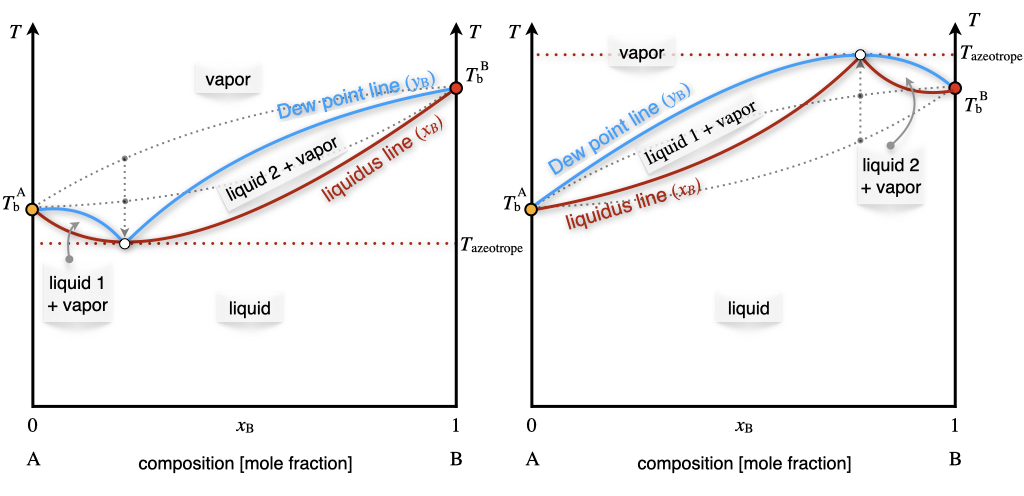
\includegraphics[width=0.8\linewidth]{./img/OEP_Figures.026} 

}

\caption{The Temperature–Composition Phase Diagram of Non-Ideal Solutions Containing Two Volatile Components at Constant Pressure.}\label{fig:FigMC8}
\end{figure}

The minimum (left plot) and maximum (right plot) points in Figure \ref{fig:FigMC8} represent the so-called \emph{azeotrope}.

An azeotrope is a constant boiling point solution whose composition cannot be altered or changed by simple distillation. This happens because the liquidus and Dew point lines coincide at this point. Therefore, the liquid and the vapor phases have the same composition, and distillation cannot occur. Two types of azeotropes exist, representative of the two types of non-ideal behavior of solutions. The first type is the positive azeotrope (left plot in Figure \ref{fig:FigMC8}). A notorious example of this behavior at atmospheric pressure is the ethanol/water mixture, with composition 95.63\% ethanol by mass. This positive azeotrope boils at \(T=78.2\;^\circ \text{C}\), a temperature that is lower than the boiling points of the pure constituents, since ethanol boils at \(T=78.4\;^\circ \text{C}\) and water at \(T=100\;^\circ \text{C}\). The second type is the negative azeotrope (right plot in Figure \ref{fig:FigMC8}). An example of this behavior at atmospheric pressure is the hydrochloric acid/water mixture with composition 20.2\% hydrochloric acid by mass. This negative azeotrope boils at \(T=110\;^\circ \text{C}\), a temperature that is higher than the boiling points of the pure constituents, since hydrochloric acid boils at \(T=-84\;^\circ \text{C}\) and water at \(T=100\;^\circ \text{C}\).

\hypertarget{phase-diagrams-of-2-components2-condensed-phases-systems}{%
\section{Phase Diagrams of 2-Components/2-Condensed Phases Systems}\label{phase-diagrams-of-2-components2-condensed-phases-systems}}

We now consider equilibria between two condensed phases: liquid/liquid, liquid/solid, and solid/solid. These equilibria usually occur in the low-temperature region of a phase diagram (or high pressure). Three situations are possible, depending on the constituents and concentration of the mixture.

\hypertarget{totally-miscible}{%
\subsection{Totally miscible}\label{totally-miscible}}

We have already encountered the situation where the components of a solution mix entirely in the liquid phase. All the diagrams that we've discussed up to this point belong to this category.

\hypertarget{totally-immiscible}{%
\subsection{Totally immiscible}\label{totally-immiscible}}

A more complicated case is that for components that do not mix in the liquid phase. The liquid region of the temperature--composition phase diagram for a solution with components that do not mix in the liquid phase below a specific temperature is reported in Figure \ref{fig:FigMC9}.

\begin{figure}

{\centering \includegraphics[width=0.6\linewidth]{./img/OEP_Figures.027} 

}

\caption{The Liquid Region of the Temperature–Composition Phase Diagram of Solutions Containing Two Components that are Completely Immiscible in the Liquid Phase.}\label{fig:FigMC9}
\end{figure}

While the liquid 1+liquid 2 region (white area in Figure \ref{fig:FigMC9}) might seem similar to the liquid region that sits on top of it (blue area in Figure \ref{fig:FigMC9}), it is substantially different in nature. To prove this, we can calculate the degrees of freedom in each region using the Gibbs phase rule. For the liquid region at the top of the diagram, at constant pressure, we have \(f=2-1+1=2\). In other words, the temperature and the composition are independent, and their values can be changed regardless of each other. In the liquid 1+liquid 2 at the bottom, however, we have \#f=2-2+1=1\$, which means that only one variable is independent of the others. The white region in Figure \ref{fig:FigMC9} is a 2-phase region, and it behaves similarly to the other 2-phases regions that we encountered before, such as the inner portion of the lens in Figure \ref{fig:FigMC4}. In other words, since the two components are entirely immiscible, once we set the temperature at a value below the immiscibility line, the concentration of the two liquid will be determined by tracing a horizontal line and by reading the concentrations on the left and right of the diagram (corresponding to 100\% \(\mathrm{A}\) and 100\% \(\mathrm{B}\), respectively).

\hypertarget{partially-miscible}{%
\subsection{Partially miscible}\label{partially-miscible}}

The third and final case is undoubtedly the most interesting since several behaviors are possible. In fact, there might be components that are partially miscible at low temperatures but totally miscible at higher temperatures, for which the diagram will assume the general shape depicted in Figure \ref{fig:FigMC10}. A typical example of this behavior is the mixture between water and phenol, whose liquids are completely miscible at \(T>66\;^\circ \text{C}\), and only partially miscible below this temperature. The composition of the 2-phases region (white area in Figure \ref{fig:FigMC10}) is determined by tracing a horizontal line and reading the mole fraction on the line that delimits the area, as for the previous case.\footnote{The only noticeable difference, in this case, is that the two concentrations will be different than 0 and 100\% since the component mix partially.}

\begin{figure}

{\centering \includegraphics[width=0.6\linewidth]{./img/OEP_Figures.028} 

}

\caption{The Liquid Region of the Temperature–Composition Phase Diagram of Solutions Containing Two Components that are Partially Immiscible at Low Temperature in the Liquid Phase, but Completely Miscible at High Temperatures}\label{fig:FigMC10}
\end{figure}

On the opposite side of the spectrum, the diagram for a mixture whose components are partially miscible at high temperature, but completely miscible at lower temperatures is depicted in Figure \ref{fig:FigMC11}. A typical example of this behavior is the mixture between water and triethylamine, whose liquids are completely miscible at \(T<18.5\;^\circ \text{C}\), and only partially miscible above this temperature.

\begin{figure}

{\centering \includegraphics[width=0.6\linewidth]{./img/OEP_Figures.029} 

}

\caption{The Liquid Region of the Temperature–Composition Phase Diagram of Solutions Containing Two Components that are Partially Immiscible at High Temperature in the Liquid Phase, but Completely Miscible at Low Temperatures.}\label{fig:FigMC11}
\end{figure}

Finally, both situations described above are possible simultaneously. For some particular solutions, there exists a range of temperature where the two components are only partially miscible. A typical example of this behavior is given by the water/nicotine mixture, whose liquids are completely miscible at \(T>210\;^\circ \text{C}\) and \(T<61\;^\circ \text{C}\), but only partially miscible in between these two temperatures, as in the diagram of Figure \ref{fig:FigMC12}.

\begin{figure}

{\centering \includegraphics[width=0.6\linewidth]{./img/OEP_Figures.030} 

}

\caption{The Liquid Region of the Temperature–Composition Phase Diagram of Solutions Containing Two Components that are Partially Immiscible Only Between Two Temperatures.}\label{fig:FigMC12}
\end{figure}

\hypertarget{eutectic-systems}{%
\subsection{Eutectic systems}\label{eutectic-systems}}

For some particular mixture, the temperature of partial miscibility in the liquid/liquid region might be close to the azeotrope temperature. In some cases, these two regions might even overlap. These characteristic behaviors are reported in Figure \ref{fig:FigMC13}.

\begin{figure}

{\centering \includegraphics[width=0.8\linewidth]{./img/OEP_Figures.031} 

}

\caption{Interaction Between the Liquid/Gas and Liquid/Liquid Equilibria.}\label{fig:FigMC13}
\end{figure}

When the azeotrope and partially miscibility temperature overlap, the system forms what is known as an \emph{eutectic}. Eutectic diagrams are possible at the liquid/gas equilibrium. Still, they are widespread at the liquid/solid equilibrium, where two components are completely miscible in the liquid phase, but only partially miscible in the solid phase. Eutectics with completely immiscible components in the solid phase are also very common, as the diagram reported in Figure \ref{fig:FigMC14}.

\begin{figure}

{\centering \includegraphics[width=0.6\linewidth]{./img/OEP_Figures.032} 

}

\caption{Typical Eutectic System with Components that are Completely Miscible in the Liquid Phase and Completely Immiscible in the Solid Phase.}\label{fig:FigMC14}
\end{figure}

\renewcommand*{\standardstate}{{-\kern-6pt{\ominus}\kern-6pt-}}

\hypertarget{Solutions}{%
\chapter{Solutions}\label{Solutions}}

In the previous chapter, we have qualitatively described the deviation of real solutions from ideal behavior. In this section, we are discussing it quantitatively. We will be able to do so by using a concept that we have already encountered in chapter \ref{ChemicalEquilibrium}: Lewis's activity.

\hypertarget{activity}{%
\section{Activity}\label{activity}}

For non-ideal gases, we introduced in chapter \ref{RealGases} the concept of \emph{fugacity} as an \emph{effective pressure} that accounts for non-ideal behavior. If we extend this concept to non-ideal solution, we can introduce the \emph{activity} of a liquid or a solid, \(a\), as:

\begin{equation}
\mu_{\text{non-ideal}} = \mu^{{-\kern-6pt{\ominus}\kern-6pt-}} + RT \ln a,
\label{eq:act1}
\end{equation}

where \(\mu\) is the chemical potential of the substance or the mixture, and \(\mu^{{-\kern-6pt{\ominus}\kern-6pt-}}\) is the chemical potential at standard state. Comparing this definition to eq. \eqref{eq:dcpnig}, it is clear that the activity is equal to the fugacity for a non-ideal gas (which, in turn, is equal to the pressure for an ideal gas). However, for a liquid and a liquid mixture, it depends on the chemical potential at standard state. This means that the activity is not an absolute quantity, but rather a relative term describing how ``active'' a compound is compared to standard state conditions. The choice of the standard state is, in principle, arbitrary, but conventions are often chosen out of mathematical or experimental convenience. We already discussed the convention that standard state for a gas is at \(P^{{-\kern-6pt{\ominus}\kern-6pt-}}=1\;\text{bar}\), so the activity is equal to the fugacity. The standard state for a component in a solution is the pure component at the temperature and pressure of the solution. This definition is equivalent to setting the activity of a pure component, \(i\), at \(a_i=1\).

For a component in a solution we can use eq. \eqref{eq:dcpnig} to write the chemical potential in the gas phase as:

\begin{equation}
\mu_i^{\text{vapor}} = \mu_i^{{-\kern-6pt{\ominus}\kern-6pt-}} + RT \ln \frac{P_i}{P^{{-\kern-6pt{\ominus}\kern-6pt-}}}.
\label{eq:act2}
\end{equation}

If the gas phase is in equilibrium with the liquid solution, then:

\begin{equation}
\mu_i^{\text{solution}} = \mu_i^{\text{vapor}} = \mu_i^*,
\label{eq:act3}
\end{equation}

where \(\mu_i^*\) is the chemical potential of the pure element. Subtracting eq. \eqref{eq:act3} from eq. \eqref{eq:act2}, we obtain:

\begin{equation}
\mu_i^{\text{solution}} = \mu_i^* + RT \ln \frac{P_i}{P^*_i}.
\label{eq:act4}
\end{equation}

For an ideal solution, we can use Raoult's law, eq. \eqref{eq:mc1}, to rewrite eq. \eqref{eq:act4} as:

\begin{equation}
\mu_i^{\text{solution}} = \mu_i^* + RT \ln x_i,
\label{eq:act5}
\end{equation}

which relates the chemical potential of a component in an ideal solution to the chemical potential of the pure liquid and its mole fraction in the solution. For a non-ideal solution, the partial pressure in eq. \eqref{eq:act4} is either larger (positive deviation) or smaller (negative deviation) than the pressure calculated using Raoult's law. The chemical potential of a component in the mixture is then calculated using:

\begin{equation}
\mu_i^{\text{solution}} = \mu_i^* + RT \ln \left(\gamma_i x_i\right),
\label{eq:act6}
\end{equation}

where \(\gamma_i\) is a positive coefficient that accounts for deviations from ideality. This coefficient is either larger than one (for positive deviations), or smaller than one (for negative deviations). The activity of component \(i\) can be calculated as an \emph{effective mole fraction}, using:

\begin{equation}
a_i = \gamma_i x_i,
\label{eq:act7}
\end{equation}

where \(\gamma_i\) is defined as the \emph{activity coefficient}. The partial pressure of the component can then be related to its vapor pressure, using:

\begin{equation}
P_i = a_i P_i^*.
\label{eq:act8}
\end{equation}

Comparing eq. \eqref{eq:act8} with Raoult's law, we can calculate the activity coefficient as:

\begin{equation}
\gamma_i = \frac{P_i}{x_i P_i^*} = \frac{P_i}{P_i^{\text{R}}},
\label{eq:act9}
\end{equation}

where \(P_i^{\text{R}}\) is the partial pressure calculated using Raoult's law. This result also proves that for an ideal solution, \(\gamma=1\). Eq. \eqref{eq:act9} can also be used experimentally to obtain the activity coefficient from the phase diagram of the non-ideal solution. This is achieved by measuring the value of the partial pressure of the vapor of a non-ideal solution. Examples of this procedure are reported for both positive and negative deviations in Figure \ref{fig:FigSol1}.

\begin{figure}

{\centering \includegraphics[width=0.8\linewidth]{./img/OEP_Figures.033} 

}

\caption{Positive and Negative Deviation from Raoult's Law in the Pressure–Composition Phase Diagram of Non-Ideal Solutions at Constant Temperature.}\label{fig:FigSol1}
\end{figure}

As we already discussed in chapter \ref{ChemicalEquilibrium}, the activity is the most general quantity that we can use to define the equilibrium constant of a reaction (or the reaction quotient). The advantage of using the activity is that it's defined for ideal and non-ideal gases and mixtures of gases, as well as for ideal and non-ideal solutions in both the liquid and the solid phase.\footnote{Notice that, since the activity is a relative measure, the equilibrium constant expressed in terms of the activities is also a relative concept. In other words, it measures equilibrium relative to a standard state. This fact, however, should not surprise us, since the equilibrium constant is also related to \(\Delta_{\text{rxn}} G^{{-\kern-6pt{\ominus}\kern-6pt-}}\) using Gibbs' relation. This is why the definition of a universally agreed-upon \href{https://en.wikipedia.org/wiki/Standard_state}{standard state} is such an essential concept in chemistry, and why it is defined by the \href{https://en.wikipedia.org/wiki/International_Union_of_Pure_and_Applied_Chemistry}{International Union of Pure and Applied Chemistry (IUPAC)} and followed systematically by chemists around the globe.}

\hypertarget{colligative-properties}{%
\section{Colligative Properties}\label{colligative-properties}}

Colligative properties are properties of solutions that depend on the number of particles in the solution and not on the nature of the chemical species. More specifically, a colligative property depends on the ratio between the number of particles of the solute and the number of particles of the solvent. This ratio can be measured using any unit of concentration, such as mole fraction, molarity, and normality. For diluted solutions, however, the most useful concentration for studying colligative properties is the molality, \(m\), which measures the ratio between the number of particles of the solute (in moles) and the mass of the solvent (in kg):

\begin{equation}
m = \frac{n_{\text{solute}}}{m_{\text{solvent}}}.
\label{eq:coll1}
\end{equation}

Colligative properties usually result from the dissolution of a nonvolatile solute in a volatile liquid solvent, and they are properties of the solvent, modified by the presence of the solute. They are physically explained by the fact that the solute particles displace some solvent molecules in the liquid phase, thereby reducing the concentration of the solvent. This explanation shows how colligative properties are independent of the nature of the chemical species in a solution only if the solution is ideal. For non-ideal solutions, the formulas that we will derive below are valid only in an approximate manner. We will discuss the following four colligative properties: relative lowering of the vapor pressure, elevation of the boiling point, depression of the freezing point, and osmotic pressure.

\hypertarget{vapor-pressure-lowering}{%
\subsection{Vapor pressure lowering}\label{vapor-pressure-lowering}}

As we have already discussed in chapter \ref{MCPhaseDiagrams}, the vapor pressure of an ideal solution follows Raoult's law. Its difference with respect to the vapor pressure of the pure solvent can be calculated as:

\begin{equation}
\begin{aligned}
P_{\text{solvent}}^* &- P_{\text{solution}} = P_{\text{solvent}}^* - x_{\text{solvent}} P_{\text{solvent}}^* \\ 
& = \left( 1-x_{\text{solvent}}\right)P_{\text{solvent}}^* =x_{\text{solute}} P_{\text{solvent}}^*,
\end{aligned}
\label{eq:coll2}
\end{equation}

which shows that the vapor pressure lowering depends only on the concentration of the solute. As such, it is a colligative property.

\hypertarget{boiling-point-elevation-and-melting-point-depression}{%
\subsection{Boiling point elevation and melting point depression}\label{boiling-point-elevation-and-melting-point-depression}}

The following two colligative properties are explained by reporting the changes due to the solute molecules in the plot of the chemical potential as a function of temperature (Figure \ref{fig:FigPhase1}).

At the boiling point, the chemical potential of the solution is equal to the chemical potential of the vapor, and the following relation can be obtained:

\begin{equation}
\begin{aligned}
\mu_{\text{solution}} &=\mu_{\text{vap}}=\mu_{\text{solvent}}^{{-\kern-6pt{\ominus}\kern-6pt-}} + RT \ln P_{\text{solvent}} \\
&= \mu_{\text{solvent}}^{{-\kern-6pt{\ominus}\kern-6pt-}} + RT \ln \left(x_{\text{solvent}} P_{\text{solvent}}^* \right)\\
&= \underbrace{\mu_{\text{solvent}}^{{-\kern-6pt{\ominus}\kern-6pt-}} + RT \ln P_{\text{solvent}}^*}_{\mu_{\text{solvent}}^*} + RT \ln x_{\text{solvent}} \\
&= \mu_{\text{solvent}}^* + RT \ln x_{\text{solvent}},
\end{aligned}
\label{eq:collA}
\end{equation}

and since \(x_{\text{solvent}}<1\), the logarithmic term in the last expression is negative, and:

\begin{equation}
\mu_{\text{solution}} < \mu_{\text{solvent}}^*. 
\label{eq:collB}
\end{equation}

Eq. \eqref{eq:collA} proves that the addition of a solute always stabilizes the solvent in the liquid phase, and lowers its chemical potential, as shown in Figure \ref{fig:FigSol2}.

\begin{figure}

{\centering \includegraphics[width=0.6\linewidth]{./img/OEP_Figures.034} 

}

\caption{Reduction of the Chemical Potential of the Liquid Phase Due to the Addition of a Solute.}\label{fig:FigSol2}
\end{figure}

The elevation of the boiling point can be quantified using:

\begin{equation}
\Delta T_{\text{b}}=T_{\text{b}}^{\text{solution}}-T_{\text{b}}^{\text{solvent}}=iK_{\text{b}}m,
\label{eq:coll3}
\end{equation}

where \(i\) is the \emph{van 't Hoff factor}, a coefficient that measures the number of solute particles for each formula unit, \(K_{\text{b}}\) is the ebullioscopic constant of the solvent, and \(m\) is the molality of the solution, as introduced in eq. \eqref{eq:coll1} above. For a solute that does not dissociate in solution, \(i=1\). For a solute that dissociates in solution, the number of particles in solutions depends on how many particles it dissociates into, and \(i>1\). For example, the strong electrolyte \(\mathrm{Ca}\mathrm{Cl}_2\) completely dissociates into three particles in solution, one \(\mathrm{Ca}^{2+}\) and two \(\mathrm{Cl}^-\), and \(i=3\). For cases of partial dissociation, such as weak acids, weak bases, and their salts, \(i\) can assume non-integer values.

If we assume ideal solution behavior,the ebullioscopic constant can be obtained from the thermodynamic condition for liquid-vapor equilibrium. At the boiling point of the solution, the chemical potential of the solvent in the solution phase equals the chemical potential in the pure vapor phase above the solution:

\begin{equation}
\mu_{\text{solution}} (T_{\text{b}})  = \mu_{\text{solvent}}^*(T_b)  + RT\ln x_{\text{solvent}},
\label{eq:coll4}
\end{equation}

from which we can derive, using the Gibbs--Helmholtz equation, eq. \eqref{eq:gibbshelm}:

\begin{equation}
K_{\text{b}}=\frac{RMT_{\text{b}}^{2}}{\Delta_{\mathrm{vap}} H},
\label{eq:coll5}
\end{equation}

where \(R\) is the ideal gas constant, \(M\) is the molar mass of the solvent, and \(\Delta_{\mathrm{vap}} H\) is its molar enthalpy of vaporization.

The reduction of the melting point is similarly obtained by:

\begin{equation}
\Delta T_{\text{m}}=T_{\text{m}}^{\text{solution}}-T_{\text{m}}^{\text{solvent}}=-iK_{\text{m}}m,
\label{eq:coll6}
\end{equation}

where \(i\) is the van 't Hoff factor introduced above, \(K_{\text{m}}\) is the \emph{cryoscopic constant} of the solvent, \(m\) is the molality, and the minus sign accounts for the fact that the melting temperature of the solution is lower than the melting temperature of the pure solvent (\(\Delta T_{\text{f}}\) is defined as a negative quantity, while \(i\), \(K_{\text{f}}\), and \(m\) are all positive). Similarly to the previous case, the cryoscopic constant can be related to the molar enthalpy of fusion of the solvent using the equivalence of the chemical potential of the solid and the liquid phases at the melting point, and employing the Gibbs--Helmholtz equation:

\begin{equation}
K_{\text{m}}=\frac{RMT_{\text{m}}^{2}}{\Delta_{\mathrm{fus}}H}.
\label{eq:coll7}
\end{equation}

Notice from Figure \ref{fig:FigSol2} how the depression of the melting point is always smaller than the elevation of the boiling point. This is because the chemical potential of the solid is essentially flat, while the chemical potential of the gas is steep. Consequently, the value of the cryoscopic constant is always bigger than the value of the ebullioscopic constant. For example, for water \(K_{\text{f}} = 1.86\; \frac{\text{K kg}}{\text{mol}}\), while \(K_{\text{b}} = 0.512\; \frac{\text{K kg}}{\text{mol}}\). This is also proven by the fact that the enthalpy of vaporization is larger than the enthalpy of fusion.

\hypertarget{osmotic-pressure}{%
\subsection{Osmotic pressure}\label{osmotic-pressure}}

The osmotic pressure of a solution is defined as the difference in pressure between the solution and the pure liquid solvent when the two are in equilibrium across a semi-permeable (osmotic) membrane. The osmotic membrane is made of a porous material that allows the flow of solvent molecules but blocks the flow of the solute ones. The osmosis process is depicted in Figure \ref{fig:FigSol3}.

\begin{figure}

{\centering \includegraphics[width=0.8\linewidth]{./img/OEP_Figures.035} 

}

\caption{Osmotic Pressure of a Solution.}\label{fig:FigSol3}
\end{figure}

Starting from a solvent at atmospheric pressure in the apparatus depicted in Figure \ref{fig:FigSol3}, we can add solute particles to the left side of the apparatus. The increase in concentration on the left causes a net transfer of solvent across the membrane. This flow stops when the pressure difference equals the osmotic pressure, \(\pi\). The formula that governs the osmotic pressure was initially proposed by van 't Hoff and later refined by Harmon Northrop Morse (1848--1920). The Morse formula reads:

\begin{equation}
\pi = imRT,
\label{eq:coll8}
\end{equation}

where \(i\) is the van 't Hoff factor introduced above, \(m\) is the molality of the solution, \(R\) is the ideal gas constant, and \(T\) the temperature of the solution. As with the other colligative properties, the Morse equation is a consequence of the equality of the chemical potentials of the solvent and the solution at equilibrium.\footnote{For a derivation, see the osmotic pressure \href{https://en.wikipedia.org/wiki/Osmotic_pressure}{Wikipedia page}.}

\hypertarget{Kinetics}{%
\chapter{Chemical Kinetics}\label{Kinetics}}

\begin{center}\rule{0.5\linewidth}{0.5pt}\end{center}

From thermodynamics, we can determine the spontaneity of a reaction and its extent, using \(\Delta G\) and \(K\), respectively. However, thermodynamics does not provide any information on how \emph{fast} the reaction is going to happen. For example, while the reaction that converts solid carbon from its diamond allotropic form into hexagonal graphite is thermodynamically spontaneous, it is so slow as to be virtually non-existent. Diamond is effectively a meta-stable phase. The speed of a chemical reaction is the subject of a branch of physical chemistry called chemical kinetics.

A chemical kinetics study aims to find the \emph{rate} of a reaction and to find the microscopic steps that compose it, determining its \emph{mechanism}.

\hypertarget{diffintk}{%
\section{Differential and integrated rate laws}\label{diffintk}}

The rate law of a chemical reaction is an equation that links the initial rate with the concentrations (or pressures) of the reactants. Rate laws usually include a constant parameter, \(k\), called the \emph{rate coefficient}, and several parameters found at the exponent of the concentrations of the reactants, and are called \emph{reaction orders}. The rate coefficient depends on several conditions, including the reaction type, the temperature, the surface area of an adsorbent, light irradiation, and others. The reaction rate is usually represented with the lowercase letter \(k\), and it should not be confused with the thermodynamic equilibrium constant that is generally designated with the uppercase letter \(K\). Another useful concept in kinetics is the half-life, usually abbreviated with \(t_{1/2}\). The half-life is defined as the time required to reach half of the initial reactant concentration.

A reaction that happens in one single microscopic step is called elementary. Elementary reactions have reaction orders equal to the (integer) stoichiometric coefficients for each reactant. As such, only a limited number of elementary reactions are possible (four types are commonly observed), and they are classified according to their overall reaction order. The global reaction order of a reaction is calculated as the sum of each reactant's individual orders and is, at most, equal to three. We examine in detail the four most common reaction orders below.

\hypertarget{zeroth-order-reaction}{%
\subsection{Zeroth-order reaction}\label{zeroth-order-reaction}}

For a zeroth-order reaction, the reaction rate is independent of the concentration of a reactant. In other words, if we have a reaction of the type:

\begin{equation}
\text{A}\longrightarrow\text{products}
\end{equation}

the differential rate law can be written:

\begin{equation}
- \frac{d[\mathrm{A}]}{dt}=k_0 [\mathrm{A}]^0 = k_0,
\label{eq:kin2}
\end{equation}

which shows that any change in the concentration of \(\mathrm{A}\) will have no effect on the speed of the reaction. The minus sign at the right-hand-side is required because the rate is always defined as a positive quantity, while the derivative is negative because the concentration of the reactant is diminishing with time.
Separating the variables \([\mathrm{A}]\) and \(t\) of eq. \eqref{eq:kin2} and integrating both sides, we obtain the integrated rate law for a zeroth-order reaction as:

\begin{equation}
\begin{aligned}
\int_{[\mathrm{A}]_0}^{[A]} d[\mathrm{A}] &= -k_0 \int_{t=0}^{t} dt \\
[\mathrm{A}]-[\mathrm{A}]_0 &= -k_0 t \\ \\
[\mathrm{A}]&=[\mathrm{A}]_0 -k_0 t.
\end{aligned}
\label{eq:kin3}
\end{equation}

Using the integrated rate law, we notice that the concentration on the reactant diminishes linearly with respect to time. A plot of \([\mathrm{A}]\) as a function of \(t\), therefore, will result in a straight line with an angular coefficient equal to \(-k_0\), as in the plot of Figure \ref{fig:figk1}.

\begin{figure}

{\centering \includegraphics{pchem1_files/figure-latex/figk1-1} 

}

\caption{Reaction Rate Plot for a Zeroth-Order Reaction.}\label{fig:figk1}
\end{figure}

Eq. \eqref{eq:kin3} also suggests that the units of the rate coefficient for a zeroth-order reaction are of concentration divided by time, typically \(\frac{\mathrm{M}}{\mathrm{s}}\), with \(\mathrm{M}\) being the molar concentration in \(\frac{\mathrm{mol}}{\mathrm{L}}\) and \(s\) the time in seconds.
The half-life of a zero order reaction can be calculated from eq. \eqref{eq:kin3}, by replacing \([\mathrm{A}]\) with \(\frac{1}{2}[\mathrm{A}]_0\):

\begin{equation}
\begin{aligned}
\frac{1}{2}[\mathrm{A}]_0 &=[\mathrm{A}]_0 -k_0 t_{1/2} \\
t_{1/2} &= \frac{[\mathrm{A}]_0}{2k_0}.
\end{aligned}
\label{eq:kin4}
\end{equation}

Zeroth-order reactions are common in several biochemical processes catalyzed by enzymes, such as the oxidation of ethanol to acetaldehyde in the liver by the alcohol dehydrogenase enzyme, which is zero-order in ethanol.

\hypertarget{first-order-reaction}{%
\subsection{First-order reaction}\label{first-order-reaction}}

A first-order reaction depends on the concentration of only one reactant, and is therefore also called a \emph{unimolecular reaction}. As for the previous case, if we consider a reaction of the type:

\begin{equation}
\mathrm{A}\rightarrow \text{products}
\end{equation}

the differential rate law for a first-order reaction is:

\begin{equation}
- \frac{d[\mathrm{A}]}{dt}=k_1 [\mathrm{A}].
\label{eq:kin6}
\end{equation}

Following the usual blueprint of separating the variables, and integrating both sides, we obtain the integrated rate law as:

\begin{equation}
\begin{aligned}
\int_{[\mathrm{A}]_0}^{[A]} \frac{d[\mathrm{A}]}{[\mathrm{A}]} &= -k_1 \int_{t=0}^{t} dt \\
\ln \frac{[\mathrm{A}]}{[\mathrm{A}]_0}&=-k_1 t\\ \\
[\mathrm{A}] &= [\mathrm{A}]_0 \exp(-k_1 t).
\end{aligned}
\label{eq:kin7}
\end{equation}

Using the integrated rate law to plot the concentration of the reactant, \([\mathrm{A}]\), as a function of time, \(t\), we obtain an exponential decay, as in Figure \ref{fig:figk2}.

\begin{figure}

{\centering \includegraphics{pchem1_files/figure-latex/figk2-1} 

}

\caption{Reaction Rate Plot for a First-Order Reaction.}\label{fig:figk2}
\end{figure}

However, if we plot the logarithm of the concentration, \(\ln[\mathrm{A}]\), as a function of time, we obtain a line with angular coefficient \(-k_1\), as in the plot of Figure \ref{fig:figk3}. From eq. \eqref{eq:kin7}, we can also obtain the units for the rate coefficient for a first-order reaction, which typically is \(\frac{1}{\mathrm{s}}\), independent of concentration. Since the rate coefficient for first-order reactions has units of inverse time, it is sometimes called the frequency rate.

\begin{figure}

{\centering \includegraphics{pchem1_files/figure-latex/figk3-1} 

}

\caption{Linear Plot for a First-Order Reaction. Notice that the Quantity on the y Axes is ln[A].}\label{fig:figk3}
\end{figure}

The half-life of a first-order reaction is:

\begin{equation}
\begin{aligned}
\ln \frac{\frac{1}{2}[\mathrm{A}]_0}{[\mathrm{A}]_0}&=-k_1 t_{1/2}\\
t_{1/2} &= \frac{\ln 2}{k_1}.
\end{aligned}
\label{eq:kin8}
\end{equation}

The half-life of a first-order reaction is independent of the initial concentration of the reactant. Therefore, the half-life can be used in place of the rate coefficient to describe the reaction rate. Typical examples of first-order reactions are radioactive decays. For radioactive isotopes, it is common to report their rate of decay in terms of their half-life. For example, the most stable uranium nucleotide, \(^{238}\mathrm{U}\), has a half-life of \(4.468\times 10^9\) years, while the most common fissile isotope of uranium, \(^{235}\mathrm{U}\), has a half-life of \(7.038\times 10^8\) years.\footnote{Notice how large these numbers are for uranium. To put these numbers in perspective, we can compare them with the half-life of the most unstable isotope of plutonium, \(^{241}\mathrm{Pu}\), which is \(t_{1/2}=14.1\) years.} Other examples of first-order reactions in chemistry are the class of S\textsubscript{N}1 nucleophilic substitution reactions in organic chemistry.

\hypertarget{second-order-reaction}{%
\subsection{Second-order reaction}\label{second-order-reaction}}

A reaction is second-order when the sum of the reaction orders is two. Elementary second-order reactions are also called \emph{bimolecular reactions}. There are two possibilities, a simple one, where the reaction order of one reagent is two, or a more complicated one, with two reagents having each a reaction order of one.

\begin{itemize}
\tightlist
\item
  For the simple case, we can write the reaction as:
  \begin{equation}
  2\mathrm{A}\rightarrow \text{products}
  \end{equation}
  the differential rate law for a first-order reaction is:
  \begin{equation}
  -\frac{d[\mathrm{A}]}{dt}=k_2 [\mathrm{A}]^2.
  \label{eq:kin10}
  \end{equation}
  Following the same procedure used for the two previous cases, we can obtain the integrated rate law as:
  \begin{equation}
  \begin{aligned}
  \int_{[\mathrm{A}]_0}^{[A]} \frac{d[\mathrm{A}]}{[\mathrm{A}]^2} &= -k_2 \int_{t=0}^{t} dt \\
  \frac{1}{[\mathrm{A}]}-\frac{1}{[\mathrm{A}]_0} &= k_2 t\\ \\
  \frac{1}{[\mathrm{A}]}&=\frac{1}{[\mathrm{A}]_0} + k_2 t.
  \end{aligned}
  \label{eq:kin11}
  \end{equation}
  As for first-order reactions, the plot of the concentration as a function of time shows a non-linear decay. However, if we plot the inverse of the concentration, \(\frac{1}{[\mathrm{A}]}\), as a function of time, \(t\), we obtain a line with angular coefficient \(+k_2\), as in the plot of Figure \ref{fig:figk4}.
\end{itemize}

\begin{figure}

{\centering \includegraphics{pchem1_files/figure-latex/figk4-1} 

}

\caption{Linear Plot for a Second-Order Reaction. Notice that the Quantity on the y Axes is 1/[A].}\label{fig:figk4}
\end{figure}

Notice that the line has a \emph{positive} angular coefficient, in contrast with the previous two cases, for which the angular coefficients were negative. The units of \(k\) for a simple second order reaction are calculated from eq. \eqref{eq:kin11} and typically are \(\frac{1}{\mathrm{M}\cdot \mathrm{s}}\).
The half-life of a simple second-order reaction is:
\begin{equation}
\begin{aligned}
\frac{1}{\frac{1}{2}[\mathrm{A}]_0}-\frac{1}{[\mathrm{A}]_0} &= k_2 t_{1/2} \\
t_{1/2} &= \frac{1}{k_2 [\mathrm{A}]_0},
\end{aligned}
\label{eq:kin12}
\end{equation}
which, perhaps not surprisingly, depends on the initial concentration of the reactant, \([\mathrm{A}]_0\). Therefore, if we start with a higher concentration of the reactant, the half-life will be shorter, and the reaction will be faster. An example of simple second-order behavior is the reaction \(\mathrm{NO}_2 + \mathrm{CO} \rightarrow \mathrm{NO} + \mathrm{CO}_2\), which is second-order in \(\mathrm{NO}_2\) and zeroth-order in \(\mathrm{CO}\).

\begin{itemize}
\tightlist
\item
  For the complex second-order case, the reaction is:
  \begin{equation}
  \mathrm{A}+\mathrm{B}\rightarrow \text{products}
  \end{equation}
  and the differential rate law is:
  \begin{equation}
  -\frac{d[\mathrm{A}]}{dt}=k'_2 [\mathrm{A}][\mathrm{B}].
  \label{eq:kin14}
  \end{equation}
  The differential equation in eq. \eqref{eq:kin14} has two variables, and cannot be solved exactly unless an additional relationship is specified. If we assume that the initial concentration of the two reactants are equal, then \([\mathrm{A}]=[\mathrm{B}]\) at any time \(t\), and eq. \eqref{eq:kin14} reduces to eq. \eqref{eq:kin10}. If the concentration of the reactants are different, then the integrated rate law will assume the following shape:
  \begin{equation}
  \frac{\mathrm{[A]}}{\mathrm{[B]}} = \frac{\mathrm{[A]_0}}{\mathrm{[B]_0}} \exp \left\{ \left(\mathrm{[A]_0} - \mathrm{[B]_0}\right) k'_2t \right\}.
  \label{eq:kin15}
  \end{equation}
  The units of \(k\) for a complex second order reaction can be calculated from eq. \eqref{eq:kin15}, and are the same as those for the simple case, \(\frac{1}{\mathrm{M}\cdot \mathrm{s}}\).
  The half-life of a complex second-order reaction cannot be easily written since two different half-lives could, in principle, be defined for each of the corresponding reactants.
\end{itemize}

\hypertarget{third-and-higher-orders-reaction}{%
\subsection{Third and higher orders reaction}\label{third-and-higher-orders-reaction}}

Although elementary reactions with order higher than two are possible, they are in practice infrequent, and only very few experimental third-order reactions are observed. Fourth-order or higher have never been observed because the probabilities for a simultaneous interaction between four molecules are essentially zero. Third-order elementary reactions are also called \emph{termolelucar reactions}. While termolelucar reactions with three identical reactants are possible in principle, there is no known experimental example. Some complex third-order reactions are known, such as:

\begin{equation}
2\text{NO}_{(g)}+\text{O}_{2(g)}\longrightarrow 2\text{NO}_{2(g)}
\end{equation}

for which the differential rate law can be written as:

\begin{equation}
-\frac{dP_{\mathrm{O}_2}}{dt}=k_3 P_{\mathrm{NO}}^2 P_{\mathrm{O}_2}.
\label{eq:kin17}
\end{equation}

\hypertarget{complex-rate-laws}{%
\section{Complex Rate Laws}\label{complex-rate-laws}}

It is essential to specify that the order of a reaction and its molecularity are equal only for elementary reactions. Reactions that follow complex laws are composed of several elementary steps, and they usually have non-integer reaction orders, for at least one of the reactants.

\hypertarget{consecutive-reactions}{%
\subsection{Consecutive reactions}\label{consecutive-reactions}}

A reaction that happens following a sequence of two elementary steps can be written as follows:

\begin{equation}
\text{A}\xrightarrow{\;k_1\;}\text{B}\xrightarrow{\;k_2\;}\text{C}
\end{equation}

Assuming that each of the steps follows a first order kinetic law, and that only the reagent \(\mathrm{A}\) is present at the beginning of the reaction, we can write the differential change in concentration of each species with respect to infinitesimal time \(dt\), using the following formulas:

\begin{equation}
\begin{aligned}
-\frac{d[\mathrm{A}]}{dt}&=k_1 [\mathrm{A}] \Rightarrow [\mathrm{A}] = [\mathrm{A}]_0 \exp(-k_1 t) \\
\frac{d[\mathrm{B}]}{dt} &=k_1 [\mathrm{A}]-k_2 [\mathrm{B}] \\
\frac{d[\mathrm{C}]}{dt} &=k_2 [\mathrm{B}].
\end{aligned}
\label{eq:kincomp2}
\end{equation}

These three equations represent a system of differential equations with three unknown variables. Unfortunately, these equations are linearly dependent on each other, and they are not sufficient to solve the system for each variable. To do so, we need to include a fourth equation, coming from the conservation of mass:

\begin{equation}
[\mathrm{A}]_0=[\mathrm{A}]+[\mathrm{B}]+[\mathrm{C}].
\label{eq:kincomp3}
\end{equation}

Using the first equation in eq. \eqref{eq:kincomp2}, we can now replace the concentration \([\mathrm{A}]\) in the second equation and solve for \([\mathrm{B}]\):

\begin{equation}
\frac{d[\mathrm{B}]}{dt}+k_2 [\mathrm{B}]=k_1 [\mathrm{A}]_0 \exp(-k_1 t),
\label{eq:kincomp4}
\end{equation}

which can be simplified by multiplying both sides by \(\exp (k_2t)\):

\begin{equation}
\begin{aligned}
\left( \frac{d[\mathrm{B}]}{dt}+k_2 [\mathrm{B}] \right) \exp (k_2t) &= k_1 [\mathrm{A}]_0 \exp[(k_2-k_1) t] \\
\Rightarrow \frac{d\left\{[\mathrm{B}]\exp (k_2t)\right\}}{dt} &= k_1 [\mathrm{A}]_0 \exp[(k_2-k_1) t],
\end{aligned}
\label{eq:kincomp5}
\end{equation}

which can then be integrated remembering that \([B]_0=0\), and \(\int \exp(kx)=\frac{1}{k}\exp(kx)\):

\begin{equation}
[\mathrm{B}] = \frac{k_1}{k_2-k_1} [\mathrm{A}]_0 [\exp(-k_1t)-\exp(-k_2t)].
\label{eq:kincomp6}
\end{equation}

We can then use both \([\mathrm{A}]\), from eq. \eqref{eq:kincomp2}, and \([\mathrm{B}]\), from eq. \eqref{eq:kincomp6}, in eq. \eqref{eq:kincomp3} to solve for \([\mathrm{C}]\):

\begin{equation}
\begin{aligned}
\left[\mathrm{C}\right] &= [\mathrm{A}]_0-[\mathrm{A}]-[\mathrm{B}] \\
&= [\mathrm{A}]_0-[\mathrm{A}]_0 \exp(-k_1 t)-\frac{k_1}{k_2-k_1} [\mathrm{A}]_0 [\exp(-k_1t)-\exp(-k_2t)] \\
&= [\mathrm{A}]_0\left\{1+\frac{-k_2 \exp(-k_1t)+ k_1 \exp(-k_2t)}{k_2-k_1} \right\}.
\end{aligned}
\label{eq:kincomp7}
\end{equation}

From these results, we can distinguish two extreme behaviors. The first one is observed when \(k_1 \cong k_2\), and it produces a plot of the concentration of species with respect to time reported in Figure \ref{fig:figk5}. This behavior is observed when a process undergoing a series of consecutive reactions present a rate-determining step in the middle of the sequence (the second reaction, in the simple case analyzed above). Once the process is established, its rate will equate the rate of the slowest step.

\begin{figure}

{\centering \includegraphics{pchem1_files/figure-latex/figk5-1} 

}

\caption{Concentration Plot for a Process with Two Consecutive Reactions with the Second One Being the Rate-Determining Step.}\label{fig:figk5}
\end{figure}

The second behavior is observed when \(k_1\ll k_2\), and it produces the plot in Figure \ref{fig:figk6} In this case, the concentration of the intermediate species \(B\) is not relevant throughout the process, and the rate-determining step is the first reaction. As such, the process has the same rate law as an elementary reaction going directly from \(A\) to \(C\).

\begin{figure}

{\centering \includegraphics{pchem1_files/figure-latex/figk6-1} 

}

\caption{Concentration Plot for a Process with Two Consecutive Reactions with the First One Being the Rate-Determining Step..}\label{fig:figk6}
\end{figure}

Since the concentration of \(B\) is small and relatively constant throughout the process, \(\frac{d[\mathrm{B}]}{dT}=0\). We can then simplify the mathematical treatment of these reactions by eliminating it from the process altogether. This simplification is known as the \emph{steady-state approximation}. It is used in chemical kinetics to study processes that undergo a series of reactions producing intermediate species whose concentrations are constants throughout the entire process.

\begin{equation}
\begin{aligned}
\text{A} &\xrightarrow{\;k_1\;} \text{I}_1 \xrightarrow{\;k_2\;} \text{I}_2 \xrightarrow{\quad} \cdots \xrightarrow{\;k_n\;}\text{products} \\
& \text{Steady State Approximation:} \\
\text{A}&\xrightarrow{\qquad\qquad\qquad\qquad\quad\quad\;\;}\text{products}
\end{aligned}
\label{eq:kincomp8}
\end{equation}

\hypertarget{competitive-reactions}{%
\subsection{Competitive reactions}\label{competitive-reactions}}

A process where two elementary reactions happen in parallel, competing with each can be written as follows:

\begin{equation}
\begin{matrix}
 &_{k_1}  & B\\
 &\nearrow & \\
A &   & \\
 &\searrow& \\
  &_{k_2}  & C
\end{matrix}
\end{equation}

Assuming that each step follows first order kinetic, we can write:

\begin{equation}
\begin{aligned}
-\frac{d[\mathrm{A}]}{dt} &=k_1 [\mathrm{A}]+k_2 [\mathrm{A}] \Rightarrow [\mathrm{A}]=[\mathrm{A}]_0\exp \left[ -(k_1+k_2)t \right] \\
\frac{d[\mathrm{B}]}{dt} &=k_1 [\mathrm{A}] \Rightarrow [\mathrm{B}]=\frac{k_1}{k_1+k_2}[\mathrm{A}]_0 \left\{ 1-\exp \left[ -(k_1+k_2)t \right] \right\} \\
\frac{d[\mathrm{C}]}{dt} &=k_2 [\mathrm{A}]\Rightarrow [\mathrm{C}]=\frac{k_2}{k_1+k_2}[\mathrm{A}]_0 \left\{ 1-\exp \left[ -(k_1+k_2)t \right] \right\}.
\end{aligned}
\label{eq:kincomp2}
\end{equation}

The concentration of each of the species can then be plotted against time, obtaining the diagram reported in Figure \ref{fig:figk7}. The final concentrations of the products, \([\mathrm{B}]_f\) and \([\mathrm{C}]_f\), will depend on the values of the two rate coefficients. For example, if \(k_1>k_2\), \([\mathrm{B}]_f>[\mathrm{C}]_f\), as in Figure \ref{fig:figk7}, but if \(k_1<k_2\), \([\mathrm{B}]_f<[\mathrm{C}]_f\).

\begin{figure}

{\centering \includegraphics{pchem1_files/figure-latex/figk7-1} 

}

\caption{Concentration Plot for a Process with Two Competitive Reactions.}\label{fig:figk7}
\end{figure}

An important relationship that can be derived from eq. \eqref{eq:kincomp2} is that:

\begin{equation}
\frac{[\mathrm{B}]}{[\mathrm{C}]} =\frac{k_1}{k_2}.
\label{eq:kincomp3}
\end{equation}

\hypertarget{opposed-reactions}{%
\subsection{Opposed reactions}\label{opposed-reactions}}

Another case of complex kinetic law happens when a pair of forward and reverse reactions occur simultaneously:

\begin{equation}
\mathrm{A}\ce{<=>[k_1][k_{-1}]}\mathrm{B}
\end{equation}

where the rate coefficients for the forward and backwards reaction, \(k_1\) and \(k_{-1}\) respectively, are not necessarily equal to each other, but comparable in magnitude. We can write the rate laws for each of these elementary steps as:

\begin{equation}
\begin{aligned}
-\frac{d[\mathrm{A}]}{dt} &=k_1 [\mathrm{A}]-k_{-1} [\mathrm{B}] = k_1 [\mathrm{A}]-k_{-1}\left([\mathrm{A}]_0-[\mathrm{A}]\right) \\
\frac{d[\mathrm{A}]}{dt} &=-(k_1+k_{-1})[\mathrm{A}] + k_{-1}[\mathrm{A}]_0,
\end{aligned}
\label{eq:kinopp1}
\end{equation}

which can then be integrated to:

\begin{equation}
\begin{aligned}
\left[\mathrm{A}\right] &=[\mathrm{A}]_0\frac{k_{-1}+k_1\exp[-(k_1+k_{-1})t]}{k_1+k_{-1}} \\
\left[\mathrm{B}\right] &=[\mathrm{A}]_0\left\{ 1-\frac{k_{-1}+k_1\exp[-(k_1+k_{-1})t]}{k_1+k_{-1}}\right\}.
\end{aligned}
\label{eq:kinopp2}
\end{equation}

These formulas can then be used to obtain the plots in Figure \ref{fig:figkK}.

\begin{figure}

{\centering \includegraphics{pchem1_files/figure-latex/figkK-1} 

}

\caption{Concentration Plot for a Process with Two Opposed Reactions.}\label{fig:figkK}
\end{figure}

As can be seen from the plots in Figure \ref{fig:figkK}, after a sufficiently long time, the systems reach a dynamic equilibrium, where the concentration of \(\mathrm{A}\) and \(\mathrm{B}\) don't change. These equilibrium concentrations can be calculated replacing \(t=\infty\) in eq. \eqref{eq:kinopp1}:

\begin{equation}
\begin{aligned}
\left[\mathrm{A} \right] _{\mathrm{eq}} &= [\mathrm{A}]_0 \frac{k_{-1}}{k_1+k_{-1}} \\
[\mathrm{B}]_{\mathrm{eq}} &= [\mathrm{A}]_0 \frac{k_{1}}{k_1+k_{-1}}.
\end{aligned}
\label{eq:kinopp3}
\end{equation}

Considering that the concentrations of the species don't change at equilibrium:

\begin{equation}
\begin{aligned}
-\frac{d[\mathrm{A}]_{\mathrm{eq}}}{dt} &= \frac{d[\mathrm{B}]_{\mathrm{eq}}}{dt} = 0\\
& \Rightarrow \; k_1[\mathrm{A}]_{\mathrm{eq}} = k_{-1}[\mathrm{B}]_{\mathrm{eq}} \\
& \Rightarrow \;  \frac{k_1}{k_{-1}} =  \frac{[\mathrm{B}]_{\mathrm{eq}}}{[\mathrm{A}]_{\mathrm{eq}}} = K_C, \\
\end{aligned}
\label{eq:kinopp4}
\end{equation}

where \(K_C\) is the equilibrium constant as defined in chapter \ref{ChemicalEquilibrium}. This is a rare link between kinetics and thermodynamics and appears only for opposed reactions after sufficient time has passed so that the system can reach the dynamic equilibrium.

\hypertarget{experimental-methods-for-determination-of-reaction-orders}{%
\section{Experimental Methods for Determination of Reaction Orders}\label{experimental-methods-for-determination-of-reaction-orders}}

To experimentally measure the reaction rate, we need a method to measure concentration changes with respect to time. The simplest way to determine the reaction rate is to monitor the entire reaction as it proceeds and then plot the resulting data differently until a linear plot is found. A summary of the results obtained in section \ref{diffintk} and that is useful for this task is reported in the following table:

\scriptsize

\begin{longtable}[]{@{}lcccc@{}}
\toprule
\begin{minipage}[b]{(\columnwidth - 4\tabcolsep) * \real{0.09}}\raggedright
\strut
\end{minipage} & \begin{minipage}[b]{(\columnwidth - 4\tabcolsep) * \real{0.17}}\centering
\emph{Zeroth-Order}\strut
\end{minipage} & \begin{minipage}[b]{(\columnwidth - 4\tabcolsep) * \real{0.15}}\centering
\emph{First-Order}\strut
\end{minipage} & \begin{minipage}[b]{(\columnwidth - 4\tabcolsep) * \real{0.19}}\centering
\emph{Simple Second-Order}\strut
\end{minipage} & \begin{minipage}[b]{(\columnwidth - 4\tabcolsep) * \real{0.40}}\centering
\emph{Complex Second-Order}\strut
\end{minipage}\tabularnewline
\midrule
\endhead
\begin{minipage}[t]{(\columnwidth - 4\tabcolsep) * \real{0.09}}\raggedright
\textbf{Differential Rate Law}\strut
\end{minipage} & \begin{minipage}[t]{(\columnwidth - 4\tabcolsep) * \real{0.17}}\centering
\(-\frac{d[\mathrm{A}]}{dt}=k_0 [\mathrm{A}]^0 = k_0\)\strut
\end{minipage} & \begin{minipage}[t]{(\columnwidth - 4\tabcolsep) * \real{0.15}}\centering
\(-\frac{d[\mathrm{A}]}{dt}=k_1 [\mathrm{A}]\)\strut
\end{minipage} & \begin{minipage}[t]{(\columnwidth - 4\tabcolsep) * \real{0.19}}\centering
\(-\frac{d[\mathrm{A}]}{dt}=k_2 [\mathrm{A}]^2\)\strut
\end{minipage} & \begin{minipage}[t]{(\columnwidth - 4\tabcolsep) * \real{0.40}}\centering
\(-\frac{d[\mathrm{A}]}{dt}=k'_2 [\mathrm{A}][\mathrm{B}]\)\strut
\end{minipage}\tabularnewline
\begin{minipage}[t]{(\columnwidth - 4\tabcolsep) * \real{0.09}}\raggedright
\textbf{Integrated Rate Law}\strut
\end{minipage} & \begin{minipage}[t]{(\columnwidth - 4\tabcolsep) * \real{0.17}}\centering
\([\mathrm{A}]=[\mathrm{A}]_0 -k_0 t\)\strut
\end{minipage} & \begin{minipage}[t]{(\columnwidth - 4\tabcolsep) * \real{0.15}}\centering
\([\mathrm{A}]=[\mathrm{A}]_0 e^{-k_1 t}\)\strut
\end{minipage} & \begin{minipage}[t]{(\columnwidth - 4\tabcolsep) * \real{0.19}}\centering
\(\frac{1}{[\mathrm{A}]}=\frac{1}{[\mathrm{A}]_0} + k_2 t\)\strut
\end{minipage} & \begin{minipage}[t]{(\columnwidth - 4\tabcolsep) * \real{0.40}}\centering
\(\frac{\mathrm{[A]}}{\mathrm{[B]}}=\frac{\mathrm{[A]_0}}{\mathrm{[B]_0}}e^{\left(\mathrm{[A]_0}-\mathrm{[B]_0}\right)k'_2t}\)\strut
\end{minipage}\tabularnewline
\begin{minipage}[t]{(\columnwidth - 4\tabcolsep) * \real{0.09}}\raggedright
\textbf{Units of \(k\)}\strut
\end{minipage} & \begin{minipage}[t]{(\columnwidth - 4\tabcolsep) * \real{0.17}}\centering
\(\frac{\mathrm{M}}{\mathrm{s}}\)\strut
\end{minipage} & \begin{minipage}[t]{(\columnwidth - 4\tabcolsep) * \real{0.15}}\centering
\(\frac{1}{\mathrm{s}}\)\strut
\end{minipage} & \begin{minipage}[t]{(\columnwidth - 4\tabcolsep) * \real{0.19}}\centering
\(\frac{1}{\mathrm{M}\cdot \mathrm{s}}\)\strut
\end{minipage} & \begin{minipage}[t]{(\columnwidth - 4\tabcolsep) * \real{0.40}}\centering
\(\frac{1}{\mathrm{M}\cdot \mathrm{s}}\)\strut
\end{minipage}\tabularnewline
\begin{minipage}[t]{(\columnwidth - 4\tabcolsep) * \real{0.09}}\raggedright
\textbf{Linear Plot vs.~\(t\)}\strut
\end{minipage} & \begin{minipage}[t]{(\columnwidth - 4\tabcolsep) * \real{0.17}}\centering
\([\mathrm{A}]\)\strut
\end{minipage} & \begin{minipage}[t]{(\columnwidth - 4\tabcolsep) * \real{0.15}}\centering
\(\ln [\mathrm{A}]\)\strut
\end{minipage} & \begin{minipage}[t]{(\columnwidth - 4\tabcolsep) * \real{0.19}}\centering
\(\frac{1}{[\mathrm{A}]}\)\strut
\end{minipage} & \begin{minipage}[t]{(\columnwidth - 4\tabcolsep) * \real{0.40}}\centering
\(\ln \frac{[\mathrm{A}]_0[\mathrm{B}]}{[\mathrm{B}]_0[\mathrm{A}]}\)\strut
\end{minipage}\tabularnewline
\begin{minipage}[t]{(\columnwidth - 4\tabcolsep) * \real{0.09}}\raggedright
\textbf{Half-life}\strut
\end{minipage} & \begin{minipage}[t]{(\columnwidth - 4\tabcolsep) * \real{0.17}}\centering
\(t_{1/2}=\frac{[\mathrm{A}]_0}{2k_0}\)\strut
\end{minipage} & \begin{minipage}[t]{(\columnwidth - 4\tabcolsep) * \real{0.15}}\centering
\(t_{1/2}=\frac{\ln 2}{k_1}\)\strut
\end{minipage} & \begin{minipage}[t]{(\columnwidth - 4\tabcolsep) * \real{0.19}}\centering
\(t_{1/2}=\frac{1}{k_2 [\mathrm{A}]_0}\)\strut
\end{minipage} & \begin{minipage}[t]{(\columnwidth - 4\tabcolsep) * \real{0.40}}\centering
not easily defined\strut
\end{minipage}\tabularnewline
\bottomrule
\end{longtable}

\normalsize

However, this method works only if the reaction has few reactants, and it requires several measurements, each of which might be complicated to make. More useful methods to determine the reaction rate are the \emph{initial rate} and the \emph{isolation} methods that we describe below.

\hypertarget{initial-rates-method}{%
\subsection{Initial rates method}\label{initial-rates-method}}

The \emph{initial rates method} involves measuring the rate of a reaction as soon as it starts before any significant change in the concentrations of the reactants occurs. The initial rate method is practical only if the reaction is reasonably slow, but it can measure the rate unambiguously when more than one reactant is involved. For example, if we have a reaction with the following stoichiometry:

\begin{equation}
\alpha \mathrm{A} + \beta \mathrm{B} \xrightarrow{k} \text{products}
\end{equation}

the initial rate method can be used to determine the coefficients of the rate law:

\begin{equation}
\text{Rate}=k[\mathrm{A}]^{\alpha}[\mathrm{B}]^{\beta}
\label{eq:kinini1}
\end{equation}

by designing three experiment, where the initial concentrations of \(\mathrm{A}\) and \(\mathrm{B}\) are appropriately changed. For example, let's consider the following experimental data from three different experiments:

\begin{longtable}[]{@{}lccc@{}}
\toprule
\begin{minipage}[b]{(\columnwidth - 3\tabcolsep) * \real{0.17}}\raggedright
\strut
\end{minipage} & \begin{minipage}[b]{(\columnwidth - 3\tabcolsep) * \real{0.23}}\centering
\([\mathrm{A}]_0 \; (\text{M})\)\strut
\end{minipage} & \begin{minipage}[b]{(\columnwidth - 3\tabcolsep) * \real{0.23}}\centering
\([\mathrm{A}]_0 \; (\text{M})\)\strut
\end{minipage} & \begin{minipage}[b]{(\columnwidth - 3\tabcolsep) * \real{0.36}}\centering
\(\text{initial rate}\;\left(\frac{M}{s}\right)\)\strut
\end{minipage}\tabularnewline
\midrule
\endhead
\begin{minipage}[t]{(\columnwidth - 3\tabcolsep) * \real{0.17}}\raggedright
\(\text{Experiment 1:}\)\strut
\end{minipage} & \begin{minipage}[t]{(\columnwidth - 3\tabcolsep) * \real{0.23}}\centering
0.10\strut
\end{minipage} & \begin{minipage}[t]{(\columnwidth - 3\tabcolsep) * \real{0.23}}\centering
0.10\strut
\end{minipage} & \begin{minipage}[t]{(\columnwidth - 3\tabcolsep) * \real{0.36}}\centering
4.32\strut
\end{minipage}\tabularnewline
\begin{minipage}[t]{(\columnwidth - 3\tabcolsep) * \real{0.17}}\raggedright
\(\text{Experiment 2:}\)\strut
\end{minipage} & \begin{minipage}[t]{(\columnwidth - 3\tabcolsep) * \real{0.23}}\centering
0.15\strut
\end{minipage} & \begin{minipage}[t]{(\columnwidth - 3\tabcolsep) * \real{0.23}}\centering
0.10\strut
\end{minipage} & \begin{minipage}[t]{(\columnwidth - 3\tabcolsep) * \real{0.36}}\centering
9.70\strut
\end{minipage}\tabularnewline
\begin{minipage}[t]{(\columnwidth - 3\tabcolsep) * \real{0.17}}\raggedright
\(\text{Experiment 3:}\)\strut
\end{minipage} & \begin{minipage}[t]{(\columnwidth - 3\tabcolsep) * \real{0.23}}\centering
0.10\strut
\end{minipage} & \begin{minipage}[t]{(\columnwidth - 3\tabcolsep) * \real{0.23}}\centering
0.20\strut
\end{minipage} & \begin{minipage}[t]{(\columnwidth - 3\tabcolsep) * \real{0.36}}\centering
4.29\strut
\end{minipage}\tabularnewline
\bottomrule
\end{longtable}

we can calculate \(\alpha\) by taking the ratio of the rates measured in experiment 1 and 2:

\begin{equation}
\begin{aligned}
\frac{\text{Rate}(1)}{\text{Rate}(2)}&=\frac{k(0.10\;\text{M})^\alpha(0.10\;\text{M})^\beta}{k(0.15\;\text{M})^\alpha(0.10\;\text{M})^\beta} \\
\frac{4.32}{9.70}&=\frac{(0.10\;\text{M})^\alpha}{(0.15\;\text{M})^\alpha} \\
0.445&=0.667^\alpha \;\rightarrow\; \ln0.445=\alpha \ln0.667 \\
\alpha &= \frac{-0.81}{-0.405}=2.
\end{aligned}
\label{eq:kiniso1}
\end{equation}

\(\beta\) can be calculated similarly by taking the ratio between experiments 1 and 3. Alternatively, we can also notice that the reaction rate does not change when the initial concentration \([\mathrm{B}]_0\) is doubled, therefore \(\beta=0\).

\hypertarget{isolation-method}{%
\subsection{Isolation method}\label{isolation-method}}

Another method that is widely used to determine reaction orders is the \emph{isolation method}. This method is performed by using large excess concentrations of all reactants but one. For example, if we have the following reaction with three reagents and unknown rate law:

\begin{equation}
\alpha \mathrm{A} + \beta \mathrm{B} + \gamma \mathrm{C} \xrightarrow{k} \text{products}
\end{equation}

we can perform three different experiments, in each of which we use an excessive amount of one of the two reagents, such as:

\begin{itemize}
\item
  Experiment 1: \([\mathrm{A}]_0=1\;\text{M},\quad [\mathrm{B}]_0=1000\;\text{M}, \quad [\mathrm{C}]_0=1000\;\text{M},\) in which the reaction order with respect to \(\mathrm{A}\) is measured.
\item
  Experiment 2: \([\mathrm{A}]_0=1000\;\text{M},\quad [\mathrm{B}]_0=1\;\text{M}, \quad [\mathrm{C}]_0=1000\;\text{M},\) in which the reaction order with respect to \(\mathrm{B}\) is measured.
\item
  Experiment 3: \([\mathrm{A}]_0=1000\;\text{M},\quad [\mathrm{B}]_0=1000\;\text{M}, \quad [\mathrm{C}]_0=1\;\text{M},\) in which the reaction order with respect to \(\mathrm{C}\) is measured.
\end{itemize}

From each experiment we can determine the \emph{pseudo-order} of the reaction with respect to the reagent that is in minority concentration. For example, for the reaction above, we can write the rate law as:

\begin{equation}
\text{Rate}=k[\mathrm{A}]^{\alpha}[\mathrm{B}]^{\beta}[\mathrm{C}]^{\gamma}
\label{eq:kiniso1}
\end{equation}

and we can write the initial concentrations, \([X]_0\), and the final concentrations, \([X]_f\), of each of the species in experiment 1, as:

\begin{equation}
\begin{aligned}
\left[\mathrm{A}\right]_0 =1\;\text{M}\;\longrightarrow &[\mathrm{A}]_f=0\;\text{M} \qquad &\text{(100\% change)} \\
\left[\mathrm{B}\right]_0 =1000\;\text{M}\;\longrightarrow &[\mathrm{B}]_f=1000-1=999\;\text{M}\cong [\mathrm{B}]_0\qquad &\text{(0.1\% change)}\\
\left[\mathrm{C}\right]_0 =1000\;\text{M}\;\longrightarrow &[\mathrm{C}]_f=1000-1=999\;\text{M} \cong \left[\mathrm{C}\right]_0. \qquad &\text{(0.1\% change)}
\end{aligned}
\end{equation}

The coefficient \(\alpha\) can then be determined by incorporating the concentration of the reactants in excess into the rate constant as:

\begin{equation}
\begin{aligned}
\text{rate}&=k[\mathrm{A}]^{\alpha}\underbrace{[\mathrm{B}]^{\beta}[\mathrm{C}]^{\gamma}}_{\text{constant}} \\
&= k'[\mathrm{A}]^{\alpha}
\end{aligned}
\end{equation}

and then determine \(\alpha\) by verifying which order the data collected for \([\mathrm{A}]\) at various time fit. This can be simply achieved by using the zero-, first-, and second-order kinetic plots, as reported in the table above. We can determine \(\beta\) and \(\gamma\) by repeating the same procedure for the data from the other two experiments. For example, if we find for a specific reaction that \(\alpha=\) 1, \(\beta=2\), and \(\gamma=0\), we can then say that the reaction is pseudo-order one in \(\mathrm{A}\), pseudo-order two in \(\mathrm{B}\), and pseudo-order zero in \(\mathrm{C}\), with an overall reaction order of three.

\hypertarget{temperature-dependence-of-the-rate-coefficients}{%
\section{Temperature Dependence of the Rate Coefficients}\label{temperature-dependence-of-the-rate-coefficients}}

The dependence of the rate coefficient, \(k\), on the temperature is given by the \textbf{Arrhenius equation}. This formula was derived by Svante August Arrhenius (1859--1927) in 1889 and is based on the simple experimental observation that every chemical process gets faster when the temperature is increased. Working on data from equilibrium reactions previously reported by van 't Hoff, Arrhenius proposed the following simple exponential formula to explain the increase of \(k\) when \(T\) is increased:

\begin{equation}
k=A\exp\left( \frac{E_a}{RT}\right),
\label{eq:Arr1}
\end{equation}

where \(A\) is the so-called Arrhenius pre-exponential factor, and \(E_a\) is the activation energy. Both of these terms are independent of temperature,\footnote{In theory, both \(A\) and \(E_a\) show a weak temperature dependence. However, they can be considered constants at most experimental conditions, since kinetic studies are usually performed in a small temperature range.} and they represent experimental quantities that are unique to each individual reaction. Since there is no known exception to the fact that a temperature increase speeds up chemical reactions, both \(A\) and \(E_a\) are always positive. The pre-exponential factor units are the same as the rate constant and will vary depending on the order of the reaction. As suggested by its name, the activation energy has units of energy per mole of substance, \(\frac{\mathrm{J}}{\mathrm{mol}}\) in SI.

The Arrhenius equation is experimentally useful in its linearized form, which is obtained from two Arrhenius experiments, taken at different temperatures. Applying eq. \eqref{eq:Arr1} to two different experiments, and taking the ratio between the results, we obtain:

\begin{equation}
\ln \frac{k_{T_2}}{k_{T_1}}=-\frac{E_a}{RT}\left(\frac{1}{T_2}-\frac{1}{T_1}\right),
\label{eq:Arr2}
\end{equation}

which gives the plot of Figure \ref{fig:figk8}, from which \(E_a\) can be determined.

\begin{figure}

{\centering \includegraphics{pchem1_files/figure-latex/figk8-1} 

}

\caption{Arrhenius Plot Obtained Using Experimental Data at Two Different Temperatures.}\label{fig:figk8}
\end{figure}

From empirical arguments, Arrhenius proposed the idea that reactants must acquire a minimum amount of energy before they can form any product. He called this amount of minimum energy the activation energy. We can motivate this assumption by plotting energy of a reaction along the reaction coordinate, as in Figure \ref{fig:figk9}.\footnote{This plot is taken from \href{https://en.wikipedia.org/wiki/Transition_state_theory}{Wikipedia}, and have been generated and distributed by Author \href{https://commons.wikimedia.org/wiki/User:Grimlock}{Grimlock} under CC-BY-SA license.} The reaction coordinate is defined as the minimum energy path that connects the reactants with the products.

\begin{figure}

{\centering \includegraphics[width=0.7\linewidth]{./img/Rxn_coordinate_diagram_5} 

}

\caption{Reaction Coordinate Diagram for a Typical Reaction.}\label{fig:figk9}
\end{figure}

\renewcommand*{\standardstate}{{-\kern-6pt{\ominus}\kern-6pt-}}

\hypertarget{appendix}{%
\chapter{Appendix}\label{appendix}}

\hypertarget{thermodynamic-data-of-inorganic-substances-at-298-k}{%
\section{Thermodynamic Data of Inorganic Substances at 298 K}\label{thermodynamic-data-of-inorganic-substances-at-298-k}}

\tiny

\begin{longtable}[]{@{}lllll@{}}
\toprule
\begin{minipage}[b]{(\columnwidth - 4\tabcolsep) * \real{0.12}}\raggedright
Substance:\strut
\end{minipage} & \begin{minipage}[b]{(\columnwidth - 4\tabcolsep) * \real{0.23}}\raggedright
\(\Delta_{\text{f}} H^{-\kern-6pt{\ominus}\kern-6pt-}\)
\(\scriptstyle{\text{[kJ/mol]}}\)\strut
\end{minipage} & \begin{minipage}[b]{(\columnwidth - 4\tabcolsep) * \real{0.23}}\raggedright
\(\Delta_{\text{f}} G^{-\kern-6pt{\ominus}\kern-6pt-}\)
\(\scriptstyle{\text{[kJ/mol]}}\)\strut
\end{minipage} & \begin{minipage}[b]{(\columnwidth - 4\tabcolsep) * \real{0.21}}\raggedright
\(S^{-\kern-6pt{\ominus}\kern-6pt-}\)
\(\scriptstyle{\text{[J/(mol K)]}}\)\strut
\end{minipage} & \begin{minipage}[b]{(\columnwidth - 4\tabcolsep) * \real{0.21}}\raggedright
\(C_P\)
\(\scriptstyle{\text{[J/(mol K)]}}\)\strut
\end{minipage}\tabularnewline
\midrule
\endhead
\begin{minipage}[t]{(\columnwidth - 4\tabcolsep) * \real{0.12}}\raggedright
Ag(g)\strut
\end{minipage} & \begin{minipage}[t]{(\columnwidth - 4\tabcolsep) * \real{0.23}}\raggedright
284.9\strut
\end{minipage} & \begin{minipage}[t]{(\columnwidth - 4\tabcolsep) * \real{0.23}}\raggedright
246\strut
\end{minipage} & \begin{minipage}[t]{(\columnwidth - 4\tabcolsep) * \real{0.21}}\raggedright
173\strut
\end{minipage} & \begin{minipage}[t]{(\columnwidth - 4\tabcolsep) * \real{0.21}}\raggedright
20.8\strut
\end{minipage}\tabularnewline
\begin{minipage}[t]{(\columnwidth - 4\tabcolsep) * \real{0.12}}\raggedright
Ag(s)\strut
\end{minipage} & \begin{minipage}[t]{(\columnwidth - 4\tabcolsep) * \real{0.23}}\raggedright
0\strut
\end{minipage} & \begin{minipage}[t]{(\columnwidth - 4\tabcolsep) * \real{0.23}}\raggedright
0\strut
\end{minipage} & \begin{minipage}[t]{(\columnwidth - 4\tabcolsep) * \real{0.21}}\raggedright
42.6\strut
\end{minipage} & \begin{minipage}[t]{(\columnwidth - 4\tabcolsep) * \real{0.21}}\raggedright
25.4\strut
\end{minipage}\tabularnewline
\begin{minipage}[t]{(\columnwidth - 4\tabcolsep) * \real{0.12}}\raggedright
Ag\textsuperscript{+}(aq)\strut
\end{minipage} & \begin{minipage}[t]{(\columnwidth - 4\tabcolsep) * \real{0.23}}\raggedright
105.8\strut
\end{minipage} & \begin{minipage}[t]{(\columnwidth - 4\tabcolsep) * \real{0.23}}\raggedright
77.1\strut
\end{minipage} & \begin{minipage}[t]{(\columnwidth - 4\tabcolsep) * \real{0.21}}\raggedright
73.5\strut
\end{minipage} & \begin{minipage}[t]{(\columnwidth - 4\tabcolsep) * \real{0.21}}\raggedright
\strut
\end{minipage}\tabularnewline
\begin{minipage}[t]{(\columnwidth - 4\tabcolsep) * \real{0.12}}\raggedright
AgCN(s)\strut
\end{minipage} & \begin{minipage}[t]{(\columnwidth - 4\tabcolsep) * \real{0.23}}\raggedright
146\strut
\end{minipage} & \begin{minipage}[t]{(\columnwidth - 4\tabcolsep) * \real{0.23}}\raggedright
156.9\strut
\end{minipage} & \begin{minipage}[t]{(\columnwidth - 4\tabcolsep) * \real{0.21}}\raggedright
107.2\strut
\end{minipage} & \begin{minipage}[t]{(\columnwidth - 4\tabcolsep) * \real{0.21}}\raggedright
66.7\strut
\end{minipage}\tabularnewline
\begin{minipage}[t]{(\columnwidth - 4\tabcolsep) * \real{0.12}}\raggedright
Ag\textsubscript{2}CO\textsubscript{3}(s)\strut
\end{minipage} & \begin{minipage}[t]{(\columnwidth - 4\tabcolsep) * \real{0.23}}\raggedright
--505.8\strut
\end{minipage} & \begin{minipage}[t]{(\columnwidth - 4\tabcolsep) * \real{0.23}}\raggedright
--436.8\strut
\end{minipage} & \begin{minipage}[t]{(\columnwidth - 4\tabcolsep) * \real{0.21}}\raggedright
167.4\strut
\end{minipage} & \begin{minipage}[t]{(\columnwidth - 4\tabcolsep) * \real{0.21}}\raggedright
112.3\strut
\end{minipage}\tabularnewline
\begin{minipage}[t]{(\columnwidth - 4\tabcolsep) * \real{0.12}}\raggedright
AgNO\textsubscript{3}(s)\strut
\end{minipage} & \begin{minipage}[t]{(\columnwidth - 4\tabcolsep) * \real{0.23}}\raggedright
--124.4\strut
\end{minipage} & \begin{minipage}[t]{(\columnwidth - 4\tabcolsep) * \real{0.23}}\raggedright
--33.4\strut
\end{minipage} & \begin{minipage}[t]{(\columnwidth - 4\tabcolsep) * \real{0.21}}\raggedright
140.9\strut
\end{minipage} & \begin{minipage}[t]{(\columnwidth - 4\tabcolsep) * \real{0.21}}\raggedright
93.1\strut
\end{minipage}\tabularnewline
\begin{minipage}[t]{(\columnwidth - 4\tabcolsep) * \real{0.12}}\raggedright
Ag\textsubscript{2}O(s)\strut
\end{minipage} & \begin{minipage}[t]{(\columnwidth - 4\tabcolsep) * \real{0.23}}\raggedright
--31.1\strut
\end{minipage} & \begin{minipage}[t]{(\columnwidth - 4\tabcolsep) * \real{0.23}}\raggedright
--11.2\strut
\end{minipage} & \begin{minipage}[t]{(\columnwidth - 4\tabcolsep) * \real{0.21}}\raggedright
121.3\strut
\end{minipage} & \begin{minipage}[t]{(\columnwidth - 4\tabcolsep) * \real{0.21}}\raggedright
65.9\strut
\end{minipage}\tabularnewline
\begin{minipage}[t]{(\columnwidth - 4\tabcolsep) * \real{0.12}}\raggedright
Ag\textsubscript{2}S(s)\strut
\end{minipage} & \begin{minipage}[t]{(\columnwidth - 4\tabcolsep) * \real{0.23}}\raggedright
--32.6\strut
\end{minipage} & \begin{minipage}[t]{(\columnwidth - 4\tabcolsep) * \real{0.23}}\raggedright
--40.7\strut
\end{minipage} & \begin{minipage}[t]{(\columnwidth - 4\tabcolsep) * \real{0.21}}\raggedright
144\strut
\end{minipage} & \begin{minipage}[t]{(\columnwidth - 4\tabcolsep) * \real{0.21}}\raggedright
76.5\strut
\end{minipage}\tabularnewline
\begin{minipage}[t]{(\columnwidth - 4\tabcolsep) * \real{0.12}}\raggedright
AgBr(s)\strut
\end{minipage} & \begin{minipage}[t]{(\columnwidth - 4\tabcolsep) * \real{0.23}}\raggedright
--100.4\strut
\end{minipage} & \begin{minipage}[t]{(\columnwidth - 4\tabcolsep) * \real{0.23}}\raggedright
--96.9\strut
\end{minipage} & \begin{minipage}[t]{(\columnwidth - 4\tabcolsep) * \real{0.21}}\raggedright
107.1\strut
\end{minipage} & \begin{minipage}[t]{(\columnwidth - 4\tabcolsep) * \real{0.21}}\raggedright
52.4\strut
\end{minipage}\tabularnewline
\begin{minipage}[t]{(\columnwidth - 4\tabcolsep) * \real{0.12}}\raggedright
AgCl(s)\strut
\end{minipage} & \begin{minipage}[t]{(\columnwidth - 4\tabcolsep) * \real{0.23}}\raggedright
--127.0\strut
\end{minipage} & \begin{minipage}[t]{(\columnwidth - 4\tabcolsep) * \real{0.23}}\raggedright
--109.8\strut
\end{minipage} & \begin{minipage}[t]{(\columnwidth - 4\tabcolsep) * \real{0.21}}\raggedright
96.3\strut
\end{minipage} & \begin{minipage}[t]{(\columnwidth - 4\tabcolsep) * \real{0.21}}\raggedright
50.8\strut
\end{minipage}\tabularnewline
\begin{minipage}[t]{(\columnwidth - 4\tabcolsep) * \real{0.12}}\raggedright
AgF(s)\strut
\end{minipage} & \begin{minipage}[t]{(\columnwidth - 4\tabcolsep) * \real{0.23}}\raggedright
--204.6\strut
\end{minipage} & \begin{minipage}[t]{(\columnwidth - 4\tabcolsep) * \real{0.23}}\raggedright
--187\strut
\end{minipage} & \begin{minipage}[t]{(\columnwidth - 4\tabcolsep) * \real{0.21}}\raggedright
84\strut
\end{minipage} & \begin{minipage}[t]{(\columnwidth - 4\tabcolsep) * \real{0.21}}\raggedright
\strut
\end{minipage}\tabularnewline
\begin{minipage}[t]{(\columnwidth - 4\tabcolsep) * \real{0.12}}\raggedright
AgI(s)\strut
\end{minipage} & \begin{minipage}[t]{(\columnwidth - 4\tabcolsep) * \real{0.23}}\raggedright
--61.8\strut
\end{minipage} & \begin{minipage}[t]{(\columnwidth - 4\tabcolsep) * \real{0.23}}\raggedright
--66.2\strut
\end{minipage} & \begin{minipage}[t]{(\columnwidth - 4\tabcolsep) * \real{0.21}}\raggedright
115.5\strut
\end{minipage} & \begin{minipage}[t]{(\columnwidth - 4\tabcolsep) * \real{0.21}}\raggedright
56.8\strut
\end{minipage}\tabularnewline
\begin{minipage}[t]{(\columnwidth - 4\tabcolsep) * \real{0.12}}\raggedright
Al(g)\strut
\end{minipage} & \begin{minipage}[t]{(\columnwidth - 4\tabcolsep) * \real{0.23}}\raggedright
330\strut
\end{minipage} & \begin{minipage}[t]{(\columnwidth - 4\tabcolsep) * \real{0.23}}\raggedright
289.4\strut
\end{minipage} & \begin{minipage}[t]{(\columnwidth - 4\tabcolsep) * \real{0.21}}\raggedright
164.6\strut
\end{minipage} & \begin{minipage}[t]{(\columnwidth - 4\tabcolsep) * \real{0.21}}\raggedright
21.4\strut
\end{minipage}\tabularnewline
\begin{minipage}[t]{(\columnwidth - 4\tabcolsep) * \real{0.12}}\raggedright
Al(s)\strut
\end{minipage} & \begin{minipage}[t]{(\columnwidth - 4\tabcolsep) * \real{0.23}}\raggedright
0\strut
\end{minipage} & \begin{minipage}[t]{(\columnwidth - 4\tabcolsep) * \real{0.23}}\raggedright
0\strut
\end{minipage} & \begin{minipage}[t]{(\columnwidth - 4\tabcolsep) * \real{0.21}}\raggedright
28.3\strut
\end{minipage} & \begin{minipage}[t]{(\columnwidth - 4\tabcolsep) * \real{0.21}}\raggedright
24.2\strut
\end{minipage}\tabularnewline
\begin{minipage}[t]{(\columnwidth - 4\tabcolsep) * \real{0.12}}\raggedright
Al\textsubscript{2}O\textsubscript{3}(s)\strut
\end{minipage} & \begin{minipage}[t]{(\columnwidth - 4\tabcolsep) * \real{0.23}}\raggedright
--1675.7\strut
\end{minipage} & \begin{minipage}[t]{(\columnwidth - 4\tabcolsep) * \real{0.23}}\raggedright
--1582.3\strut
\end{minipage} & \begin{minipage}[t]{(\columnwidth - 4\tabcolsep) * \real{0.21}}\raggedright
50.9\strut
\end{minipage} & \begin{minipage}[t]{(\columnwidth - 4\tabcolsep) * \real{0.21}}\raggedright
79.0\strut
\end{minipage}\tabularnewline
\begin{minipage}[t]{(\columnwidth - 4\tabcolsep) * \real{0.12}}\raggedright
AlF\textsubscript{3}(s)\strut
\end{minipage} & \begin{minipage}[t]{(\columnwidth - 4\tabcolsep) * \real{0.23}}\raggedright
--1510.4\strut
\end{minipage} & \begin{minipage}[t]{(\columnwidth - 4\tabcolsep) * \real{0.23}}\raggedright
--1431.1\strut
\end{minipage} & \begin{minipage}[t]{(\columnwidth - 4\tabcolsep) * \real{0.21}}\raggedright
66.5\strut
\end{minipage} & \begin{minipage}[t]{(\columnwidth - 4\tabcolsep) * \real{0.21}}\raggedright
75.1\strut
\end{minipage}\tabularnewline
\begin{minipage}[t]{(\columnwidth - 4\tabcolsep) * \real{0.12}}\raggedright
AlI\textsubscript{3}(s)\strut
\end{minipage} & \begin{minipage}[t]{(\columnwidth - 4\tabcolsep) * \real{0.23}}\raggedright
--302.9\strut
\end{minipage} & \begin{minipage}[t]{(\columnwidth - 4\tabcolsep) * \real{0.23}}\raggedright
\strut
\end{minipage} & \begin{minipage}[t]{(\columnwidth - 4\tabcolsep) * \real{0.21}}\raggedright
195.9\strut
\end{minipage} & \begin{minipage}[t]{(\columnwidth - 4\tabcolsep) * \real{0.21}}\raggedright
\strut
\end{minipage}\tabularnewline
\begin{minipage}[t]{(\columnwidth - 4\tabcolsep) * \real{0.12}}\raggedright
AlBr\textsubscript{3}(s)\strut
\end{minipage} & \begin{minipage}[t]{(\columnwidth - 4\tabcolsep) * \real{0.23}}\raggedright
--527.2\strut
\end{minipage} & \begin{minipage}[t]{(\columnwidth - 4\tabcolsep) * \real{0.23}}\raggedright
\strut
\end{minipage} & \begin{minipage}[t]{(\columnwidth - 4\tabcolsep) * \real{0.21}}\raggedright
180.2\strut
\end{minipage} & \begin{minipage}[t]{(\columnwidth - 4\tabcolsep) * \real{0.21}}\raggedright
100.6\strut
\end{minipage}\tabularnewline
\begin{minipage}[t]{(\columnwidth - 4\tabcolsep) * \real{0.12}}\raggedright
AlCl\textsubscript{3}(s)\strut
\end{minipage} & \begin{minipage}[t]{(\columnwidth - 4\tabcolsep) * \real{0.23}}\raggedright
--704.5\strut
\end{minipage} & \begin{minipage}[t]{(\columnwidth - 4\tabcolsep) * \real{0.23}}\raggedright
--628.11\strut
\end{minipage} & \begin{minipage}[t]{(\columnwidth - 4\tabcolsep) * \real{0.21}}\raggedright
112.3\strut
\end{minipage} & \begin{minipage}[t]{(\columnwidth - 4\tabcolsep) * \real{0.21}}\raggedright
91.1\strut
\end{minipage}\tabularnewline
\begin{minipage}[t]{(\columnwidth - 4\tabcolsep) * \real{0.12}}\raggedright
Al(OH)\textsubscript{3}(s)\strut
\end{minipage} & \begin{minipage}[t]{(\columnwidth - 4\tabcolsep) * \real{0.23}}\raggedright
--1277\strut
\end{minipage} & \begin{minipage}[t]{(\columnwidth - 4\tabcolsep) * \real{0.23}}\raggedright
\strut
\end{minipage} & \begin{minipage}[t]{(\columnwidth - 4\tabcolsep) * \real{0.21}}\raggedright
\strut
\end{minipage} & \begin{minipage}[t]{(\columnwidth - 4\tabcolsep) * \real{0.21}}\raggedright
\strut
\end{minipage}\tabularnewline
\begin{minipage}[t]{(\columnwidth - 4\tabcolsep) * \real{0.12}}\raggedright
Al(OH)\textsubscript{4}\textsuperscript{-}(aq)\strut
\end{minipage} & \begin{minipage}[t]{(\columnwidth - 4\tabcolsep) * \real{0.23}}\raggedright
--1490\strut
\end{minipage} & \begin{minipage}[t]{(\columnwidth - 4\tabcolsep) * \real{0.23}}\raggedright
--1297\strut
\end{minipage} & \begin{minipage}[t]{(\columnwidth - 4\tabcolsep) * \real{0.21}}\raggedright
117\strut
\end{minipage} & \begin{minipage}[t]{(\columnwidth - 4\tabcolsep) * \real{0.21}}\raggedright
\strut
\end{minipage}\tabularnewline
\begin{minipage}[t]{(\columnwidth - 4\tabcolsep) * \real{0.12}}\raggedright
AlPO\textsubscript{4}(s)\strut
\end{minipage} & \begin{minipage}[t]{(\columnwidth - 4\tabcolsep) * \real{0.23}}\raggedright
--1733.8\strut
\end{minipage} & \begin{minipage}[t]{(\columnwidth - 4\tabcolsep) * \real{0.23}}\raggedright
--1617.9\strut
\end{minipage} & \begin{minipage}[t]{(\columnwidth - 4\tabcolsep) * \real{0.21}}\raggedright
90.8\strut
\end{minipage} & \begin{minipage}[t]{(\columnwidth - 4\tabcolsep) * \real{0.21}}\raggedright
93.2\strut
\end{minipage}\tabularnewline
\begin{minipage}[t]{(\columnwidth - 4\tabcolsep) * \real{0.12}}\raggedright
Ar(g)\strut
\end{minipage} & \begin{minipage}[t]{(\columnwidth - 4\tabcolsep) * \real{0.23}}\raggedright
0\strut
\end{minipage} & \begin{minipage}[t]{(\columnwidth - 4\tabcolsep) * \real{0.23}}\raggedright
\strut
\end{minipage} & \begin{minipage}[t]{(\columnwidth - 4\tabcolsep) * \real{0.21}}\raggedright
154.9\strut
\end{minipage} & \begin{minipage}[t]{(\columnwidth - 4\tabcolsep) * \real{0.21}}\raggedright
20.8\strut
\end{minipage}\tabularnewline
\begin{minipage}[t]{(\columnwidth - 4\tabcolsep) * \real{0.12}}\raggedright
B(s)\strut
\end{minipage} & \begin{minipage}[t]{(\columnwidth - 4\tabcolsep) * \real{0.23}}\raggedright
0\strut
\end{minipage} & \begin{minipage}[t]{(\columnwidth - 4\tabcolsep) * \real{0.23}}\raggedright
0\strut
\end{minipage} & \begin{minipage}[t]{(\columnwidth - 4\tabcolsep) * \real{0.21}}\raggedright
5.9\strut
\end{minipage} & \begin{minipage}[t]{(\columnwidth - 4\tabcolsep) * \real{0.21}}\raggedright
11.1\strut
\end{minipage}\tabularnewline
\begin{minipage}[t]{(\columnwidth - 4\tabcolsep) * \real{0.12}}\raggedright
B(g)\strut
\end{minipage} & \begin{minipage}[t]{(\columnwidth - 4\tabcolsep) * \real{0.23}}\raggedright
565\strut
\end{minipage} & \begin{minipage}[t]{(\columnwidth - 4\tabcolsep) * \real{0.23}}\raggedright
521.0\strut
\end{minipage} & \begin{minipage}[t]{(\columnwidth - 4\tabcolsep) * \real{0.21}}\raggedright
153.4\strut
\end{minipage} & \begin{minipage}[t]{(\columnwidth - 4\tabcolsep) * \real{0.21}}\raggedright
20.8\strut
\end{minipage}\tabularnewline
\begin{minipage}[t]{(\columnwidth - 4\tabcolsep) * \real{0.12}}\raggedright
BH(g)\strut
\end{minipage} & \begin{minipage}[t]{(\columnwidth - 4\tabcolsep) * \real{0.23}}\raggedright
442.7\strut
\end{minipage} & \begin{minipage}[t]{(\columnwidth - 4\tabcolsep) * \real{0.23}}\raggedright
412.7\strut
\end{minipage} & \begin{minipage}[t]{(\columnwidth - 4\tabcolsep) * \real{0.21}}\raggedright
171.8\strut
\end{minipage} & \begin{minipage}[t]{(\columnwidth - 4\tabcolsep) * \real{0.21}}\raggedright
29.2\strut
\end{minipage}\tabularnewline
\begin{minipage}[t]{(\columnwidth - 4\tabcolsep) * \real{0.12}}\raggedright
BH\textsubscript{3}(g)\strut
\end{minipage} & \begin{minipage}[t]{(\columnwidth - 4\tabcolsep) * \real{0.23}}\raggedright
89.2\strut
\end{minipage} & \begin{minipage}[t]{(\columnwidth - 4\tabcolsep) * \real{0.23}}\raggedright
93.3\strut
\end{minipage} & \begin{minipage}[t]{(\columnwidth - 4\tabcolsep) * \real{0.21}}\raggedright
188.2\strut
\end{minipage} & \begin{minipage}[t]{(\columnwidth - 4\tabcolsep) * \real{0.21}}\raggedright
36.0\strut
\end{minipage}\tabularnewline
\begin{minipage}[t]{(\columnwidth - 4\tabcolsep) * \real{0.12}}\raggedright
B\textsubscript{2}S\textsubscript{3}(s)\strut
\end{minipage} & \begin{minipage}[t]{(\columnwidth - 4\tabcolsep) * \real{0.23}}\raggedright
--240.6\strut
\end{minipage} & \begin{minipage}[t]{(\columnwidth - 4\tabcolsep) * \real{0.23}}\raggedright
\strut
\end{minipage} & \begin{minipage}[t]{(\columnwidth - 4\tabcolsep) * \real{0.21}}\raggedright
100.0\strut
\end{minipage} & \begin{minipage}[t]{(\columnwidth - 4\tabcolsep) * \real{0.21}}\raggedright
111.7\strut
\end{minipage}\tabularnewline
\begin{minipage}[t]{(\columnwidth - 4\tabcolsep) * \real{0.12}}\raggedright
Ba(g)\strut
\end{minipage} & \begin{minipage}[t]{(\columnwidth - 4\tabcolsep) * \real{0.23}}\raggedright
180\strut
\end{minipage} & \begin{minipage}[t]{(\columnwidth - 4\tabcolsep) * \real{0.23}}\raggedright
146\strut
\end{minipage} & \begin{minipage}[t]{(\columnwidth - 4\tabcolsep) * \real{0.21}}\raggedright
170.2\strut
\end{minipage} & \begin{minipage}[t]{(\columnwidth - 4\tabcolsep) * \real{0.21}}\raggedright
\strut
\end{minipage}\tabularnewline
\begin{minipage}[t]{(\columnwidth - 4\tabcolsep) * \real{0.12}}\raggedright
Ba(s)\strut
\end{minipage} & \begin{minipage}[t]{(\columnwidth - 4\tabcolsep) * \real{0.23}}\raggedright
0\strut
\end{minipage} & \begin{minipage}[t]{(\columnwidth - 4\tabcolsep) * \real{0.23}}\raggedright
0\strut
\end{minipage} & \begin{minipage}[t]{(\columnwidth - 4\tabcolsep) * \real{0.21}}\raggedright
62.5\strut
\end{minipage} & \begin{minipage}[t]{(\columnwidth - 4\tabcolsep) * \real{0.21}}\raggedright
28.1\strut
\end{minipage}\tabularnewline
\begin{minipage}[t]{(\columnwidth - 4\tabcolsep) * \real{0.12}}\raggedright
BaCO\textsubscript{3}(s)\strut
\end{minipage} & \begin{minipage}[t]{(\columnwidth - 4\tabcolsep) * \real{0.23}}\raggedright
--1213.0\strut
\end{minipage} & \begin{minipage}[t]{(\columnwidth - 4\tabcolsep) * \real{0.23}}\raggedright
--1134.4\strut
\end{minipage} & \begin{minipage}[t]{(\columnwidth - 4\tabcolsep) * \real{0.21}}\raggedright
112.1\strut
\end{minipage} & \begin{minipage}[t]{(\columnwidth - 4\tabcolsep) * \real{0.21}}\raggedright
86.0\strut
\end{minipage}\tabularnewline
\begin{minipage}[t]{(\columnwidth - 4\tabcolsep) * \real{0.12}}\raggedright
BaH\textsubscript{2}(s)\strut
\end{minipage} & \begin{minipage}[t]{(\columnwidth - 4\tabcolsep) * \real{0.23}}\raggedright
--177\strut
\end{minipage} & \begin{minipage}[t]{(\columnwidth - 4\tabcolsep) * \real{0.23}}\raggedright
--138.2\strut
\end{minipage} & \begin{minipage}[t]{(\columnwidth - 4\tabcolsep) * \real{0.21}}\raggedright
63.0\strut
\end{minipage} & \begin{minipage}[t]{(\columnwidth - 4\tabcolsep) * \real{0.21}}\raggedright
\strut
\end{minipage}\tabularnewline
\begin{minipage}[t]{(\columnwidth - 4\tabcolsep) * \real{0.12}}\raggedright
BaBr\textsubscript{2}(s)\strut
\end{minipage} & \begin{minipage}[t]{(\columnwidth - 4\tabcolsep) * \real{0.23}}\raggedright
--757.3\strut
\end{minipage} & \begin{minipage}[t]{(\columnwidth - 4\tabcolsep) * \real{0.23}}\raggedright
--736.8\strut
\end{minipage} & \begin{minipage}[t]{(\columnwidth - 4\tabcolsep) * \real{0.21}}\raggedright
146.0\strut
\end{minipage} & \begin{minipage}[t]{(\columnwidth - 4\tabcolsep) * \real{0.21}}\raggedright
\strut
\end{minipage}\tabularnewline
\begin{minipage}[t]{(\columnwidth - 4\tabcolsep) * \real{0.12}}\raggedright
BaCl\textsubscript{2}(s)\strut
\end{minipage} & \begin{minipage}[t]{(\columnwidth - 4\tabcolsep) * \real{0.23}}\raggedright
--855\strut
\end{minipage} & \begin{minipage}[t]{(\columnwidth - 4\tabcolsep) * \real{0.23}}\raggedright
--806.7\strut
\end{minipage} & \begin{minipage}[t]{(\columnwidth - 4\tabcolsep) * \real{0.21}}\raggedright
123.7\strut
\end{minipage} & \begin{minipage}[t]{(\columnwidth - 4\tabcolsep) * \real{0.21}}\raggedright
75.1\strut
\end{minipage}\tabularnewline
\begin{minipage}[t]{(\columnwidth - 4\tabcolsep) * \real{0.12}}\raggedright
BaF\textsubscript{2}(s)\strut
\end{minipage} & \begin{minipage}[t]{(\columnwidth - 4\tabcolsep) * \real{0.23}}\raggedright
--1207.1\strut
\end{minipage} & \begin{minipage}[t]{(\columnwidth - 4\tabcolsep) * \real{0.23}}\raggedright
--1156.8\strut
\end{minipage} & \begin{minipage}[t]{(\columnwidth - 4\tabcolsep) * \real{0.21}}\raggedright
96.4\strut
\end{minipage} & \begin{minipage}[t]{(\columnwidth - 4\tabcolsep) * \real{0.21}}\raggedright
71.2\strut
\end{minipage}\tabularnewline
\begin{minipage}[t]{(\columnwidth - 4\tabcolsep) * \real{0.12}}\raggedright
BaI\textsubscript{2}(s)\strut
\end{minipage} & \begin{minipage}[t]{(\columnwidth - 4\tabcolsep) * \real{0.23}}\raggedright
--602.1\strut
\end{minipage} & \begin{minipage}[t]{(\columnwidth - 4\tabcolsep) * \real{0.23}}\raggedright
--597\strut
\end{minipage} & \begin{minipage}[t]{(\columnwidth - 4\tabcolsep) * \real{0.21}}\raggedright
167.0\strut
\end{minipage} & \begin{minipage}[t]{(\columnwidth - 4\tabcolsep) * \real{0.21}}\raggedright
\strut
\end{minipage}\tabularnewline
\begin{minipage}[t]{(\columnwidth - 4\tabcolsep) * \real{0.12}}\raggedright
BaO(s)\strut
\end{minipage} & \begin{minipage}[t]{(\columnwidth - 4\tabcolsep) * \real{0.23}}\raggedright
--548.0\strut
\end{minipage} & \begin{minipage}[t]{(\columnwidth - 4\tabcolsep) * \real{0.23}}\raggedright
--520.3\strut
\end{minipage} & \begin{minipage}[t]{(\columnwidth - 4\tabcolsep) * \real{0.21}}\raggedright
72.1\strut
\end{minipage} & \begin{minipage}[t]{(\columnwidth - 4\tabcolsep) * \real{0.21}}\raggedright
47.3\strut
\end{minipage}\tabularnewline
\begin{minipage}[t]{(\columnwidth - 4\tabcolsep) * \real{0.12}}\raggedright
BaSO\textsubscript{4}(s)\strut
\end{minipage} & \begin{minipage}[t]{(\columnwidth - 4\tabcolsep) * \real{0.23}}\raggedright
--1473.2\strut
\end{minipage} & \begin{minipage}[t]{(\columnwidth - 4\tabcolsep) * \real{0.23}}\raggedright
--1362.2\strut
\end{minipage} & \begin{minipage}[t]{(\columnwidth - 4\tabcolsep) * \real{0.21}}\raggedright
132.2\strut
\end{minipage} & \begin{minipage}[t]{(\columnwidth - 4\tabcolsep) * \real{0.21}}\raggedright
101.8\strut
\end{minipage}\tabularnewline
\begin{minipage}[t]{(\columnwidth - 4\tabcolsep) * \real{0.12}}\raggedright
Be(g)\strut
\end{minipage} & \begin{minipage}[t]{(\columnwidth - 4\tabcolsep) * \real{0.23}}\raggedright
324\strut
\end{minipage} & \begin{minipage}[t]{(\columnwidth - 4\tabcolsep) * \real{0.23}}\raggedright
286.6\strut
\end{minipage} & \begin{minipage}[t]{(\columnwidth - 4\tabcolsep) * \real{0.21}}\raggedright
136.3\strut
\end{minipage} & \begin{minipage}[t]{(\columnwidth - 4\tabcolsep) * \real{0.21}}\raggedright
20.8\strut
\end{minipage}\tabularnewline
\begin{minipage}[t]{(\columnwidth - 4\tabcolsep) * \real{0.12}}\raggedright
Be(s)\strut
\end{minipage} & \begin{minipage}[t]{(\columnwidth - 4\tabcolsep) * \real{0.23}}\raggedright
0\strut
\end{minipage} & \begin{minipage}[t]{(\columnwidth - 4\tabcolsep) * \real{0.23}}\raggedright
0\strut
\end{minipage} & \begin{minipage}[t]{(\columnwidth - 4\tabcolsep) * \real{0.21}}\raggedright
9.5\strut
\end{minipage} & \begin{minipage}[t]{(\columnwidth - 4\tabcolsep) * \real{0.21}}\raggedright
13.4\strut
\end{minipage}\tabularnewline
\begin{minipage}[t]{(\columnwidth - 4\tabcolsep) * \real{0.12}}\raggedright
BeBr\textsubscript{2}(s)\strut
\end{minipage} & \begin{minipage}[t]{(\columnwidth - 4\tabcolsep) * \real{0.23}}\raggedright
--353.5\strut
\end{minipage} & \begin{minipage}[t]{(\columnwidth - 4\tabcolsep) * \real{0.23}}\raggedright
\strut
\end{minipage} & \begin{minipage}[t]{(\columnwidth - 4\tabcolsep) * \real{0.21}}\raggedright
108\strut
\end{minipage} & \begin{minipage}[t]{(\columnwidth - 4\tabcolsep) * \real{0.21}}\raggedright
69.4\strut
\end{minipage}\tabularnewline
\begin{minipage}[t]{(\columnwidth - 4\tabcolsep) * \real{0.12}}\raggedright
BeCl\textsubscript{2}(s)\strut
\end{minipage} & \begin{minipage}[t]{(\columnwidth - 4\tabcolsep) * \real{0.23}}\raggedright
--490.4\strut
\end{minipage} & \begin{minipage}[t]{(\columnwidth - 4\tabcolsep) * \real{0.23}}\raggedright
--445.6\strut
\end{minipage} & \begin{minipage}[t]{(\columnwidth - 4\tabcolsep) * \real{0.21}}\raggedright
75.8\strut
\end{minipage} & \begin{minipage}[t]{(\columnwidth - 4\tabcolsep) * \real{0.21}}\raggedright
62.4\strut
\end{minipage}\tabularnewline
\begin{minipage}[t]{(\columnwidth - 4\tabcolsep) * \real{0.12}}\raggedright
BeF\textsubscript{2}(s)\strut
\end{minipage} & \begin{minipage}[t]{(\columnwidth - 4\tabcolsep) * \real{0.23}}\raggedright
--1026.8\strut
\end{minipage} & \begin{minipage}[t]{(\columnwidth - 4\tabcolsep) * \real{0.23}}\raggedright
--979.4\strut
\end{minipage} & \begin{minipage}[t]{(\columnwidth - 4\tabcolsep) * \real{0.21}}\raggedright
53.4\strut
\end{minipage} & \begin{minipage}[t]{(\columnwidth - 4\tabcolsep) * \real{0.21}}\raggedright
51.8\strut
\end{minipage}\tabularnewline
\begin{minipage}[t]{(\columnwidth - 4\tabcolsep) * \real{0.12}}\raggedright
BeI\textsubscript{2}(s)\strut
\end{minipage} & \begin{minipage}[t]{(\columnwidth - 4\tabcolsep) * \real{0.23}}\raggedright
--192.5\strut
\end{minipage} & \begin{minipage}[t]{(\columnwidth - 4\tabcolsep) * \real{0.23}}\raggedright
\strut
\end{minipage} & \begin{minipage}[t]{(\columnwidth - 4\tabcolsep) * \real{0.21}}\raggedright
121\strut
\end{minipage} & \begin{minipage}[t]{(\columnwidth - 4\tabcolsep) * \real{0.21}}\raggedright
71.1\strut
\end{minipage}\tabularnewline
\begin{minipage}[t]{(\columnwidth - 4\tabcolsep) * \real{0.12}}\raggedright
BeO(s)\strut
\end{minipage} & \begin{minipage}[t]{(\columnwidth - 4\tabcolsep) * \real{0.23}}\raggedright
--609.4\strut
\end{minipage} & \begin{minipage}[t]{(\columnwidth - 4\tabcolsep) * \real{0.23}}\raggedright
--580.1\strut
\end{minipage} & \begin{minipage}[t]{(\columnwidth - 4\tabcolsep) * \real{0.21}}\raggedright
13.8\strut
\end{minipage} & \begin{minipage}[t]{(\columnwidth - 4\tabcolsep) * \real{0.21}}\raggedright
25.6\strut
\end{minipage}\tabularnewline
\begin{minipage}[t]{(\columnwidth - 4\tabcolsep) * \real{0.12}}\raggedright
Be(OH)\textsubscript{2}(s)\strut
\end{minipage} & \begin{minipage}[t]{(\columnwidth - 4\tabcolsep) * \real{0.23}}\raggedright
--902.5\strut
\end{minipage} & \begin{minipage}[t]{(\columnwidth - 4\tabcolsep) * \real{0.23}}\raggedright
--815.0\strut
\end{minipage} & \begin{minipage}[t]{(\columnwidth - 4\tabcolsep) * \real{0.21}}\raggedright
45.5\strut
\end{minipage} & \begin{minipage}[t]{(\columnwidth - 4\tabcolsep) * \real{0.21}}\raggedright
62.1\strut
\end{minipage}\tabularnewline
\begin{minipage}[t]{(\columnwidth - 4\tabcolsep) * \real{0.12}}\raggedright
BeSO\textsubscript{4}(s)\strut
\end{minipage} & \begin{minipage}[t]{(\columnwidth - 4\tabcolsep) * \real{0.23}}\raggedright
--1205.2\strut
\end{minipage} & \begin{minipage}[t]{(\columnwidth - 4\tabcolsep) * \real{0.23}}\raggedright
--1093.8\strut
\end{minipage} & \begin{minipage}[t]{(\columnwidth - 4\tabcolsep) * \real{0.21}}\raggedright
77.9\strut
\end{minipage} & \begin{minipage}[t]{(\columnwidth - 4\tabcolsep) * \real{0.21}}\raggedright
85.7\strut
\end{minipage}\tabularnewline
\begin{minipage}[t]{(\columnwidth - 4\tabcolsep) * \real{0.12}}\raggedright
Bi(g)\strut
\end{minipage} & \begin{minipage}[t]{(\columnwidth - 4\tabcolsep) * \real{0.23}}\raggedright
207.1\strut
\end{minipage} & \begin{minipage}[t]{(\columnwidth - 4\tabcolsep) * \real{0.23}}\raggedright
168.2\strut
\end{minipage} & \begin{minipage}[t]{(\columnwidth - 4\tabcolsep) * \real{0.21}}\raggedright
187\strut
\end{minipage} & \begin{minipage}[t]{(\columnwidth - 4\tabcolsep) * \real{0.21}}\raggedright
20.8\strut
\end{minipage}\tabularnewline
\begin{minipage}[t]{(\columnwidth - 4\tabcolsep) * \real{0.12}}\raggedright
Bi(s)\strut
\end{minipage} & \begin{minipage}[t]{(\columnwidth - 4\tabcolsep) * \real{0.23}}\raggedright
0\strut
\end{minipage} & \begin{minipage}[t]{(\columnwidth - 4\tabcolsep) * \real{0.23}}\raggedright
0\strut
\end{minipage} & \begin{minipage}[t]{(\columnwidth - 4\tabcolsep) * \real{0.21}}\raggedright
56.7\strut
\end{minipage} & \begin{minipage}[t]{(\columnwidth - 4\tabcolsep) * \real{0.21}}\raggedright
25.5\strut
\end{minipage}\tabularnewline
\begin{minipage}[t]{(\columnwidth - 4\tabcolsep) * \real{0.12}}\raggedright
Bi\textsubscript{2}O\textsubscript{3}(s)\strut
\end{minipage} & \begin{minipage}[t]{(\columnwidth - 4\tabcolsep) * \real{0.23}}\raggedright
--573.9\strut
\end{minipage} & \begin{minipage}[t]{(\columnwidth - 4\tabcolsep) * \real{0.23}}\raggedright
--493.7\strut
\end{minipage} & \begin{minipage}[t]{(\columnwidth - 4\tabcolsep) * \real{0.21}}\raggedright
151.5\strut
\end{minipage} & \begin{minipage}[t]{(\columnwidth - 4\tabcolsep) * \real{0.21}}\raggedright
113.5\strut
\end{minipage}\tabularnewline
\begin{minipage}[t]{(\columnwidth - 4\tabcolsep) * \real{0.12}}\raggedright
BiCl\textsubscript{3}(s)\strut
\end{minipage} & \begin{minipage}[t]{(\columnwidth - 4\tabcolsep) * \real{0.23}}\raggedright
--379.1\strut
\end{minipage} & \begin{minipage}[t]{(\columnwidth - 4\tabcolsep) * \real{0.23}}\raggedright
--315.0\strut
\end{minipage} & \begin{minipage}[t]{(\columnwidth - 4\tabcolsep) * \real{0.21}}\raggedright
177.0\strut
\end{minipage} & \begin{minipage}[t]{(\columnwidth - 4\tabcolsep) * \real{0.21}}\raggedright
105.0\strut
\end{minipage}\tabularnewline
\begin{minipage}[t]{(\columnwidth - 4\tabcolsep) * \real{0.12}}\raggedright
Br\textsuperscript{--}(aq)\strut
\end{minipage} & \begin{minipage}[t]{(\columnwidth - 4\tabcolsep) * \real{0.23}}\raggedright
--121.4\strut
\end{minipage} & \begin{minipage}[t]{(\columnwidth - 4\tabcolsep) * \real{0.23}}\raggedright
--104.0\strut
\end{minipage} & \begin{minipage}[t]{(\columnwidth - 4\tabcolsep) * \real{0.21}}\raggedright
82.6\strut
\end{minipage} & \begin{minipage}[t]{(\columnwidth - 4\tabcolsep) * \real{0.21}}\raggedright
\strut
\end{minipage}\tabularnewline
\begin{minipage}[t]{(\columnwidth - 4\tabcolsep) * \real{0.12}}\raggedright
Br(g)\strut
\end{minipage} & \begin{minipage}[t]{(\columnwidth - 4\tabcolsep) * \real{0.23}}\raggedright
111.9\strut
\end{minipage} & \begin{minipage}[t]{(\columnwidth - 4\tabcolsep) * \real{0.23}}\raggedright
82.4\strut
\end{minipage} & \begin{minipage}[t]{(\columnwidth - 4\tabcolsep) * \real{0.21}}\raggedright
175\strut
\end{minipage} & \begin{minipage}[t]{(\columnwidth - 4\tabcolsep) * \real{0.21}}\raggedright
20.8\strut
\end{minipage}\tabularnewline
\begin{minipage}[t]{(\columnwidth - 4\tabcolsep) * \real{0.12}}\raggedright
Br\textsubscript{2}(g)\strut
\end{minipage} & \begin{minipage}[t]{(\columnwidth - 4\tabcolsep) * \real{0.23}}\raggedright
30.9\strut
\end{minipage} & \begin{minipage}[t]{(\columnwidth - 4\tabcolsep) * \real{0.23}}\raggedright
3.1\strut
\end{minipage} & \begin{minipage}[t]{(\columnwidth - 4\tabcolsep) * \real{0.21}}\raggedright
245.5\strut
\end{minipage} & \begin{minipage}[t]{(\columnwidth - 4\tabcolsep) * \real{0.21}}\raggedright
36.0\strut
\end{minipage}\tabularnewline
\begin{minipage}[t]{(\columnwidth - 4\tabcolsep) * \real{0.12}}\raggedright
Br\textsubscript{2}(l)\strut
\end{minipage} & \begin{minipage}[t]{(\columnwidth - 4\tabcolsep) * \real{0.23}}\raggedright
0\strut
\end{minipage} & \begin{minipage}[t]{(\columnwidth - 4\tabcolsep) * \real{0.23}}\raggedright
0\strut
\end{minipage} & \begin{minipage}[t]{(\columnwidth - 4\tabcolsep) * \real{0.21}}\raggedright
152.2\strut
\end{minipage} & \begin{minipage}[t]{(\columnwidth - 4\tabcolsep) * \real{0.21}}\raggedright
75.7\strut
\end{minipage}\tabularnewline
\begin{minipage}[t]{(\columnwidth - 4\tabcolsep) * \real{0.12}}\raggedright
BrCl(g)\strut
\end{minipage} & \begin{minipage}[t]{(\columnwidth - 4\tabcolsep) * \real{0.23}}\raggedright
14.6\strut
\end{minipage} & \begin{minipage}[t]{(\columnwidth - 4\tabcolsep) * \real{0.23}}\raggedright
--1\strut
\end{minipage} & \begin{minipage}[t]{(\columnwidth - 4\tabcolsep) * \real{0.21}}\raggedright
240.1\strut
\end{minipage} & \begin{minipage}[t]{(\columnwidth - 4\tabcolsep) * \real{0.21}}\raggedright
35.0\strut
\end{minipage}\tabularnewline
\begin{minipage}[t]{(\columnwidth - 4\tabcolsep) * \real{0.12}}\raggedright
BrF(g)\strut
\end{minipage} & \begin{minipage}[t]{(\columnwidth - 4\tabcolsep) * \real{0.23}}\raggedright
--93.8\strut
\end{minipage} & \begin{minipage}[t]{(\columnwidth - 4\tabcolsep) * \real{0.23}}\raggedright
--109.2\strut
\end{minipage} & \begin{minipage}[t]{(\columnwidth - 4\tabcolsep) * \real{0.21}}\raggedright
229\strut
\end{minipage} & \begin{minipage}[t]{(\columnwidth - 4\tabcolsep) * \real{0.21}}\raggedright
33.0\strut
\end{minipage}\tabularnewline
\begin{minipage}[t]{(\columnwidth - 4\tabcolsep) * \real{0.12}}\raggedright
BrF\textsubscript{3}(g)\strut
\end{minipage} & \begin{minipage}[t]{(\columnwidth - 4\tabcolsep) * \real{0.23}}\raggedright
--1136\strut
\end{minipage} & \begin{minipage}[t]{(\columnwidth - 4\tabcolsep) * \real{0.23}}\raggedright
1119.4\strut
\end{minipage} & \begin{minipage}[t]{(\columnwidth - 4\tabcolsep) * \real{0.21}}\raggedright
254.4\strut
\end{minipage} & \begin{minipage}[t]{(\columnwidth - 4\tabcolsep) * \real{0.21}}\raggedright
66.6\strut
\end{minipage}\tabularnewline
\begin{minipage}[t]{(\columnwidth - 4\tabcolsep) * \real{0.12}}\raggedright
C(g)\strut
\end{minipage} & \begin{minipage}[t]{(\columnwidth - 4\tabcolsep) * \real{0.23}}\raggedright
716.7\strut
\end{minipage} & \begin{minipage}[t]{(\columnwidth - 4\tabcolsep) * \real{0.23}}\raggedright
671.3\strut
\end{minipage} & \begin{minipage}[t]{(\columnwidth - 4\tabcolsep) * \real{0.21}}\raggedright
158.1\strut
\end{minipage} & \begin{minipage}[t]{(\columnwidth - 4\tabcolsep) * \real{0.21}}\raggedright
0.8\strut
\end{minipage}\tabularnewline
\begin{minipage}[t]{(\columnwidth - 4\tabcolsep) * \real{0.12}}\raggedright
C(s,diamond)\strut
\end{minipage} & \begin{minipage}[t]{(\columnwidth - 4\tabcolsep) * \real{0.23}}\raggedright
1.9\strut
\end{minipage} & \begin{minipage}[t]{(\columnwidth - 4\tabcolsep) * \real{0.23}}\raggedright
2.9\strut
\end{minipage} & \begin{minipage}[t]{(\columnwidth - 4\tabcolsep) * \real{0.21}}\raggedright
2.4\strut
\end{minipage} & \begin{minipage}[t]{(\columnwidth - 4\tabcolsep) * \real{0.21}}\raggedright
6.1\strut
\end{minipage}\tabularnewline
\begin{minipage}[t]{(\columnwidth - 4\tabcolsep) * \real{0.12}}\raggedright
C(s,graphite)\strut
\end{minipage} & \begin{minipage}[t]{(\columnwidth - 4\tabcolsep) * \real{0.23}}\raggedright
0\strut
\end{minipage} & \begin{minipage}[t]{(\columnwidth - 4\tabcolsep) * \real{0.23}}\raggedright
0\strut
\end{minipage} & \begin{minipage}[t]{(\columnwidth - 4\tabcolsep) * \real{0.21}}\raggedright
5.7\strut
\end{minipage} & \begin{minipage}[t]{(\columnwidth - 4\tabcolsep) * \real{0.21}}\raggedright
8.5\strut
\end{minipage}\tabularnewline
\begin{minipage}[t]{(\columnwidth - 4\tabcolsep) * \real{0.12}}\raggedright
CBr\textsubscript{4}(g)\strut
\end{minipage} & \begin{minipage}[t]{(\columnwidth - 4\tabcolsep) * \real{0.23}}\raggedright
83.9\strut
\end{minipage} & \begin{minipage}[t]{(\columnwidth - 4\tabcolsep) * \real{0.23}}\raggedright
67\strut
\end{minipage} & \begin{minipage}[t]{(\columnwidth - 4\tabcolsep) * \real{0.21}}\raggedright
358.1\strut
\end{minipage} & \begin{minipage}[t]{(\columnwidth - 4\tabcolsep) * \real{0.21}}\raggedright
\strut
\end{minipage}\tabularnewline
\begin{minipage}[t]{(\columnwidth - 4\tabcolsep) * \real{0.12}}\raggedright
CBr\textsubscript{4}(s)\strut
\end{minipage} & \begin{minipage}[t]{(\columnwidth - 4\tabcolsep) * \real{0.23}}\raggedright
29.4\strut
\end{minipage} & \begin{minipage}[t]{(\columnwidth - 4\tabcolsep) * \real{0.23}}\raggedright
47.7\strut
\end{minipage} & \begin{minipage}[t]{(\columnwidth - 4\tabcolsep) * \real{0.21}}\raggedright
212.5\strut
\end{minipage} & \begin{minipage}[t]{(\columnwidth - 4\tabcolsep) * \real{0.21}}\raggedright
\strut
\end{minipage}\tabularnewline
\begin{minipage}[t]{(\columnwidth - 4\tabcolsep) * \real{0.12}}\raggedright
CCl\textsubscript{2}F\textsubscript{2}(g)\strut
\end{minipage} & \begin{minipage}[t]{(\columnwidth - 4\tabcolsep) * \real{0.23}}\raggedright
--477.4\strut
\end{minipage} & \begin{minipage}[t]{(\columnwidth - 4\tabcolsep) * \real{0.23}}\raggedright
--439.4\strut
\end{minipage} & \begin{minipage}[t]{(\columnwidth - 4\tabcolsep) * \real{0.21}}\raggedright
300.8\strut
\end{minipage} & \begin{minipage}[t]{(\columnwidth - 4\tabcolsep) * \real{0.21}}\raggedright
\strut
\end{minipage}\tabularnewline
\begin{minipage}[t]{(\columnwidth - 4\tabcolsep) * \real{0.12}}\raggedright
CCl\textsubscript{2}O(g)\strut
\end{minipage} & \begin{minipage}[t]{(\columnwidth - 4\tabcolsep) * \real{0.23}}\raggedright
--219.1\strut
\end{minipage} & \begin{minipage}[t]{(\columnwidth - 4\tabcolsep) * \real{0.23}}\raggedright
--204.9\strut
\end{minipage} & \begin{minipage}[t]{(\columnwidth - 4\tabcolsep) * \real{0.21}}\raggedright
283.5\strut
\end{minipage} & \begin{minipage}[t]{(\columnwidth - 4\tabcolsep) * \real{0.21}}\raggedright
\strut
\end{minipage}\tabularnewline
\begin{minipage}[t]{(\columnwidth - 4\tabcolsep) * \real{0.12}}\raggedright
CCl\textsubscript{4}(g)\strut
\end{minipage} & \begin{minipage}[t]{(\columnwidth - 4\tabcolsep) * \real{0.23}}\raggedright
--95.7\strut
\end{minipage} & \begin{minipage}[t]{(\columnwidth - 4\tabcolsep) * \real{0.23}}\raggedright
--53.6\strut
\end{minipage} & \begin{minipage}[t]{(\columnwidth - 4\tabcolsep) * \real{0.21}}\raggedright
309.9\strut
\end{minipage} & \begin{minipage}[t]{(\columnwidth - 4\tabcolsep) * \real{0.21}}\raggedright
\strut
\end{minipage}\tabularnewline
\begin{minipage}[t]{(\columnwidth - 4\tabcolsep) * \real{0.12}}\raggedright
CCl\textsubscript{4}(l)\strut
\end{minipage} & \begin{minipage}[t]{(\columnwidth - 4\tabcolsep) * \real{0.23}}\raggedright
--128.2\strut
\end{minipage} & \begin{minipage}[t]{(\columnwidth - 4\tabcolsep) * \real{0.23}}\raggedright
--62.6\strut
\end{minipage} & \begin{minipage}[t]{(\columnwidth - 4\tabcolsep) * \real{0.21}}\raggedright
216.2\strut
\end{minipage} & \begin{minipage}[t]{(\columnwidth - 4\tabcolsep) * \real{0.21}}\raggedright
\strut
\end{minipage}\tabularnewline
\begin{minipage}[t]{(\columnwidth - 4\tabcolsep) * \real{0.12}}\raggedright
CF\textsubscript{4}(g)\strut
\end{minipage} & \begin{minipage}[t]{(\columnwidth - 4\tabcolsep) * \real{0.23}}\raggedright
--933.6\strut
\end{minipage} & \begin{minipage}[t]{(\columnwidth - 4\tabcolsep) * \real{0.23}}\raggedright
--888.3\strut
\end{minipage} & \begin{minipage}[t]{(\columnwidth - 4\tabcolsep) * \real{0.21}}\raggedright
261.6\strut
\end{minipage} & \begin{minipage}[t]{(\columnwidth - 4\tabcolsep) * \real{0.21}}\raggedright
\strut
\end{minipage}\tabularnewline
\begin{minipage}[t]{(\columnwidth - 4\tabcolsep) * \real{0.12}}\raggedright
CS\textsubscript{2}(g)\strut
\end{minipage} & \begin{minipage}[t]{(\columnwidth - 4\tabcolsep) * \real{0.23}}\raggedright
116.7\strut
\end{minipage} & \begin{minipage}[t]{(\columnwidth - 4\tabcolsep) * \real{0.23}}\raggedright
67.1\strut
\end{minipage} & \begin{minipage}[t]{(\columnwidth - 4\tabcolsep) * \real{0.21}}\raggedright
237.8\strut
\end{minipage} & \begin{minipage}[t]{(\columnwidth - 4\tabcolsep) * \real{0.21}}\raggedright
45.4\strut
\end{minipage}\tabularnewline
\begin{minipage}[t]{(\columnwidth - 4\tabcolsep) * \real{0.12}}\raggedright
CS\textsubscript{2}(l)\strut
\end{minipage} & \begin{minipage}[t]{(\columnwidth - 4\tabcolsep) * \real{0.23}}\raggedright
89\strut
\end{minipage} & \begin{minipage}[t]{(\columnwidth - 4\tabcolsep) * \real{0.23}}\raggedright
64.6\strut
\end{minipage} & \begin{minipage}[t]{(\columnwidth - 4\tabcolsep) * \real{0.21}}\raggedright
151.3\strut
\end{minipage} & \begin{minipage}[t]{(\columnwidth - 4\tabcolsep) * \real{0.21}}\raggedright
76.4\strut
\end{minipage}\tabularnewline
\begin{minipage}[t]{(\columnwidth - 4\tabcolsep) * \real{0.12}}\raggedright
CO(g)\strut
\end{minipage} & \begin{minipage}[t]{(\columnwidth - 4\tabcolsep) * \real{0.23}}\raggedright
--110.5\strut
\end{minipage} & \begin{minipage}[t]{(\columnwidth - 4\tabcolsep) * \real{0.23}}\raggedright
--137.2\strut
\end{minipage} & \begin{minipage}[t]{(\columnwidth - 4\tabcolsep) * \real{0.21}}\raggedright
197.7\strut
\end{minipage} & \begin{minipage}[t]{(\columnwidth - 4\tabcolsep) * \real{0.21}}\raggedright
29.1\strut
\end{minipage}\tabularnewline
\begin{minipage}[t]{(\columnwidth - 4\tabcolsep) * \real{0.12}}\raggedright
CO\textsubscript{2}(g)\strut
\end{minipage} & \begin{minipage}[t]{(\columnwidth - 4\tabcolsep) * \real{0.23}}\raggedright
--393.5\strut
\end{minipage} & \begin{minipage}[t]{(\columnwidth - 4\tabcolsep) * \real{0.23}}\raggedright
--394.4\strut
\end{minipage} & \begin{minipage}[t]{(\columnwidth - 4\tabcolsep) * \real{0.21}}\raggedright
213.8\strut
\end{minipage} & \begin{minipage}[t]{(\columnwidth - 4\tabcolsep) * \real{0.21}}\raggedright
37.1\strut
\end{minipage}\tabularnewline
\begin{minipage}[t]{(\columnwidth - 4\tabcolsep) * \real{0.12}}\raggedright
Ca(g)\strut
\end{minipage} & \begin{minipage}[t]{(\columnwidth - 4\tabcolsep) * \real{0.23}}\raggedright
177.8\strut
\end{minipage} & \begin{minipage}[t]{(\columnwidth - 4\tabcolsep) * \real{0.23}}\raggedright
144\strut
\end{minipage} & \begin{minipage}[t]{(\columnwidth - 4\tabcolsep) * \real{0.21}}\raggedright
154.9\strut
\end{minipage} & \begin{minipage}[t]{(\columnwidth - 4\tabcolsep) * \real{0.21}}\raggedright
20.8\strut
\end{minipage}\tabularnewline
\begin{minipage}[t]{(\columnwidth - 4\tabcolsep) * \real{0.12}}\raggedright
Ca(s)\strut
\end{minipage} & \begin{minipage}[t]{(\columnwidth - 4\tabcolsep) * \real{0.23}}\raggedright
0\strut
\end{minipage} & \begin{minipage}[t]{(\columnwidth - 4\tabcolsep) * \real{0.23}}\raggedright
0\strut
\end{minipage} & \begin{minipage}[t]{(\columnwidth - 4\tabcolsep) * \real{0.21}}\raggedright
41.6\strut
\end{minipage} & \begin{minipage}[t]{(\columnwidth - 4\tabcolsep) * \real{0.21}}\raggedright
25.9\strut
\end{minipage}\tabularnewline
\begin{minipage}[t]{(\columnwidth - 4\tabcolsep) * \real{0.12}}\raggedright
Ca(OH)\textsubscript{2}(s)\strut
\end{minipage} & \begin{minipage}[t]{(\columnwidth - 4\tabcolsep) * \real{0.23}}\raggedright
--985.2\strut
\end{minipage} & \begin{minipage}[t]{(\columnwidth - 4\tabcolsep) * \real{0.23}}\raggedright
--897.5\strut
\end{minipage} & \begin{minipage}[t]{(\columnwidth - 4\tabcolsep) * \real{0.21}}\raggedright
83.4\strut
\end{minipage} & \begin{minipage}[t]{(\columnwidth - 4\tabcolsep) * \real{0.21}}\raggedright
87.5\strut
\end{minipage}\tabularnewline
\begin{minipage}[t]{(\columnwidth - 4\tabcolsep) * \real{0.12}}\raggedright
CaBr\textsubscript{2}(s)\strut
\end{minipage} & \begin{minipage}[t]{(\columnwidth - 4\tabcolsep) * \real{0.23}}\raggedright
--682.8\strut
\end{minipage} & \begin{minipage}[t]{(\columnwidth - 4\tabcolsep) * \real{0.23}}\raggedright
--663.6\strut
\end{minipage} & \begin{minipage}[t]{(\columnwidth - 4\tabcolsep) * \real{0.21}}\raggedright
130\strut
\end{minipage} & \begin{minipage}[t]{(\columnwidth - 4\tabcolsep) * \real{0.21}}\raggedright
\strut
\end{minipage}\tabularnewline
\begin{minipage}[t]{(\columnwidth - 4\tabcolsep) * \real{0.12}}\raggedright
CaCl\textsubscript{2}(s)\strut
\end{minipage} & \begin{minipage}[t]{(\columnwidth - 4\tabcolsep) * \real{0.23}}\raggedright
--795.4\strut
\end{minipage} & \begin{minipage}[t]{(\columnwidth - 4\tabcolsep) * \real{0.23}}\raggedright
--748.8\strut
\end{minipage} & \begin{minipage}[t]{(\columnwidth - 4\tabcolsep) * \real{0.21}}\raggedright
108.4\strut
\end{minipage} & \begin{minipage}[t]{(\columnwidth - 4\tabcolsep) * \real{0.21}}\raggedright
72.9\strut
\end{minipage}\tabularnewline
\begin{minipage}[t]{(\columnwidth - 4\tabcolsep) * \real{0.12}}\raggedright
CaCN(s)\strut
\end{minipage} & \begin{minipage}[t]{(\columnwidth - 4\tabcolsep) * \real{0.23}}\raggedright
--184.5\strut
\end{minipage} & \begin{minipage}[t]{(\columnwidth - 4\tabcolsep) * \real{0.23}}\raggedright
\strut
\end{minipage} & \begin{minipage}[t]{(\columnwidth - 4\tabcolsep) * \real{0.21}}\raggedright
\strut
\end{minipage} & \begin{minipage}[t]{(\columnwidth - 4\tabcolsep) * \real{0.21}}\raggedright
\strut
\end{minipage}\tabularnewline
\begin{minipage}[t]{(\columnwidth - 4\tabcolsep) * \real{0.12}}\raggedright
CaCO\textsubscript{3}(s,arag.)\strut
\end{minipage} & \begin{minipage}[t]{(\columnwidth - 4\tabcolsep) * \real{0.23}}\raggedright
--1207.8\strut
\end{minipage} & \begin{minipage}[t]{(\columnwidth - 4\tabcolsep) * \real{0.23}}\raggedright
--1128.2\strut
\end{minipage} & \begin{minipage}[t]{(\columnwidth - 4\tabcolsep) * \real{0.21}}\raggedright
88\strut
\end{minipage} & \begin{minipage}[t]{(\columnwidth - 4\tabcolsep) * \real{0.21}}\raggedright
82.3\strut
\end{minipage}\tabularnewline
\begin{minipage}[t]{(\columnwidth - 4\tabcolsep) * \real{0.12}}\raggedright
CaCO\textsubscript{3}(s,calc.)\strut
\end{minipage} & \begin{minipage}[t]{(\columnwidth - 4\tabcolsep) * \real{0.23}}\raggedright
--1207.6\strut
\end{minipage} & \begin{minipage}[t]{(\columnwidth - 4\tabcolsep) * \real{0.23}}\raggedright
--1129.1\strut
\end{minipage} & \begin{minipage}[t]{(\columnwidth - 4\tabcolsep) * \real{0.21}}\raggedright
91.7\strut
\end{minipage} & \begin{minipage}[t]{(\columnwidth - 4\tabcolsep) * \real{0.21}}\raggedright
83.5\strut
\end{minipage}\tabularnewline
\begin{minipage}[t]{(\columnwidth - 4\tabcolsep) * \real{0.12}}\raggedright
CaF\textsubscript{2}(s)\strut
\end{minipage} & \begin{minipage}[t]{(\columnwidth - 4\tabcolsep) * \real{0.23}}\raggedright
--1228.0\strut
\end{minipage} & \begin{minipage}[t]{(\columnwidth - 4\tabcolsep) * \real{0.23}}\raggedright
--1175.6\strut
\end{minipage} & \begin{minipage}[t]{(\columnwidth - 4\tabcolsep) * \real{0.21}}\raggedright
68.5\strut
\end{minipage} & \begin{minipage}[t]{(\columnwidth - 4\tabcolsep) * \real{0.21}}\raggedright
67.0\strut
\end{minipage}\tabularnewline
\begin{minipage}[t]{(\columnwidth - 4\tabcolsep) * \real{0.12}}\raggedright
CaH\textsubscript{2}(s)\strut
\end{minipage} & \begin{minipage}[t]{(\columnwidth - 4\tabcolsep) * \real{0.23}}\raggedright
--181.5\strut
\end{minipage} & \begin{minipage}[t]{(\columnwidth - 4\tabcolsep) * \real{0.23}}\raggedright
--142.5\strut
\end{minipage} & \begin{minipage}[t]{(\columnwidth - 4\tabcolsep) * \real{0.21}}\raggedright
41.4\strut
\end{minipage} & \begin{minipage}[t]{(\columnwidth - 4\tabcolsep) * \real{0.21}}\raggedright
41.0\strut
\end{minipage}\tabularnewline
\begin{minipage}[t]{(\columnwidth - 4\tabcolsep) * \real{0.12}}\raggedright
CaI\textsubscript{2}(s)\strut
\end{minipage} & \begin{minipage}[t]{(\columnwidth - 4\tabcolsep) * \real{0.23}}\raggedright
--533.5\strut
\end{minipage} & \begin{minipage}[t]{(\columnwidth - 4\tabcolsep) * \real{0.23}}\raggedright
--528.9\strut
\end{minipage} & \begin{minipage}[t]{(\columnwidth - 4\tabcolsep) * \real{0.21}}\raggedright
142\strut
\end{minipage} & \begin{minipage}[t]{(\columnwidth - 4\tabcolsep) * \real{0.21}}\raggedright
\strut
\end{minipage}\tabularnewline
\begin{minipage}[t]{(\columnwidth - 4\tabcolsep) * \real{0.12}}\raggedright
CaO(s)\strut
\end{minipage} & \begin{minipage}[t]{(\columnwidth - 4\tabcolsep) * \real{0.23}}\raggedright
--634.9\strut
\end{minipage} & \begin{minipage}[t]{(\columnwidth - 4\tabcolsep) * \real{0.23}}\raggedright
--603.3\strut
\end{minipage} & \begin{minipage}[t]{(\columnwidth - 4\tabcolsep) * \real{0.21}}\raggedright
38.1\strut
\end{minipage} & \begin{minipage}[t]{(\columnwidth - 4\tabcolsep) * \real{0.21}}\raggedright
42.0\strut
\end{minipage}\tabularnewline
\begin{minipage}[t]{(\columnwidth - 4\tabcolsep) * \real{0.12}}\raggedright
CaSO\textsubscript{4}(s)\strut
\end{minipage} & \begin{minipage}[t]{(\columnwidth - 4\tabcolsep) * \real{0.23}}\raggedright
--1434.5\strut
\end{minipage} & \begin{minipage}[t]{(\columnwidth - 4\tabcolsep) * \real{0.23}}\raggedright
--1322.0\strut
\end{minipage} & \begin{minipage}[t]{(\columnwidth - 4\tabcolsep) * \real{0.21}}\raggedright
106.5\strut
\end{minipage} & \begin{minipage}[t]{(\columnwidth - 4\tabcolsep) * \real{0.21}}\raggedright
99.7\strut
\end{minipage}\tabularnewline
\begin{minipage}[t]{(\columnwidth - 4\tabcolsep) * \real{0.12}}\raggedright
Cd(g)\strut
\end{minipage} & \begin{minipage}[t]{(\columnwidth - 4\tabcolsep) * \real{0.23}}\raggedright
111.8\strut
\end{minipage} & \begin{minipage}[t]{(\columnwidth - 4\tabcolsep) * \real{0.23}}\raggedright
\strut
\end{minipage} & \begin{minipage}[t]{(\columnwidth - 4\tabcolsep) * \real{0.21}}\raggedright
167.7\strut
\end{minipage} & \begin{minipage}[t]{(\columnwidth - 4\tabcolsep) * \real{0.21}}\raggedright
20.8\strut
\end{minipage}\tabularnewline
\begin{minipage}[t]{(\columnwidth - 4\tabcolsep) * \real{0.12}}\raggedright
Cd(s)\strut
\end{minipage} & \begin{minipage}[t]{(\columnwidth - 4\tabcolsep) * \real{0.23}}\raggedright
0\strut
\end{minipage} & \begin{minipage}[t]{(\columnwidth - 4\tabcolsep) * \real{0.23}}\raggedright
0\strut
\end{minipage} & \begin{minipage}[t]{(\columnwidth - 4\tabcolsep) * \real{0.21}}\raggedright
51.8\strut
\end{minipage} & \begin{minipage}[t]{(\columnwidth - 4\tabcolsep) * \real{0.21}}\raggedright
26.0\strut
\end{minipage}\tabularnewline
\begin{minipage}[t]{(\columnwidth - 4\tabcolsep) * \real{0.12}}\raggedright
CdBr\textsubscript{2}(s)\strut
\end{minipage} & \begin{minipage}[t]{(\columnwidth - 4\tabcolsep) * \real{0.23}}\raggedright
--316.2\strut
\end{minipage} & \begin{minipage}[t]{(\columnwidth - 4\tabcolsep) * \real{0.23}}\raggedright
--296.3\strut
\end{minipage} & \begin{minipage}[t]{(\columnwidth - 4\tabcolsep) * \real{0.21}}\raggedright
137.2\strut
\end{minipage} & \begin{minipage}[t]{(\columnwidth - 4\tabcolsep) * \real{0.21}}\raggedright
76.7\strut
\end{minipage}\tabularnewline
\begin{minipage}[t]{(\columnwidth - 4\tabcolsep) * \real{0.12}}\raggedright
CdCl\textsubscript{2}(s)\strut
\end{minipage} & \begin{minipage}[t]{(\columnwidth - 4\tabcolsep) * \real{0.23}}\raggedright
--391.5\strut
\end{minipage} & \begin{minipage}[t]{(\columnwidth - 4\tabcolsep) * \real{0.23}}\raggedright
--343.9\strut
\end{minipage} & \begin{minipage}[t]{(\columnwidth - 4\tabcolsep) * \real{0.21}}\raggedright
115.3\strut
\end{minipage} & \begin{minipage}[t]{(\columnwidth - 4\tabcolsep) * \real{0.21}}\raggedright
74.7\strut
\end{minipage}\tabularnewline
\begin{minipage}[t]{(\columnwidth - 4\tabcolsep) * \real{0.12}}\raggedright
CdCO\textsubscript{3}(s)\strut
\end{minipage} & \begin{minipage}[t]{(\columnwidth - 4\tabcolsep) * \real{0.23}}\raggedright
--750.6\strut
\end{minipage} & \begin{minipage}[t]{(\columnwidth - 4\tabcolsep) * \real{0.23}}\raggedright
--669.4\strut
\end{minipage} & \begin{minipage}[t]{(\columnwidth - 4\tabcolsep) * \real{0.21}}\raggedright
92.5\strut
\end{minipage} & \begin{minipage}[t]{(\columnwidth - 4\tabcolsep) * \real{0.21}}\raggedright
\strut
\end{minipage}\tabularnewline
\begin{minipage}[t]{(\columnwidth - 4\tabcolsep) * \real{0.12}}\raggedright
CdF\textsubscript{2}(s)\strut
\end{minipage} & \begin{minipage}[t]{(\columnwidth - 4\tabcolsep) * \real{0.23}}\raggedright
--700.4\strut
\end{minipage} & \begin{minipage}[t]{(\columnwidth - 4\tabcolsep) * \real{0.23}}\raggedright
--647.7\strut
\end{minipage} & \begin{minipage}[t]{(\columnwidth - 4\tabcolsep) * \real{0.21}}\raggedright
77.4\strut
\end{minipage} & \begin{minipage}[t]{(\columnwidth - 4\tabcolsep) * \real{0.21}}\raggedright
\strut
\end{minipage}\tabularnewline
\begin{minipage}[t]{(\columnwidth - 4\tabcolsep) * \real{0.12}}\raggedright
CdS(s)\strut
\end{minipage} & \begin{minipage}[t]{(\columnwidth - 4\tabcolsep) * \real{0.23}}\raggedright
--161.9\strut
\end{minipage} & \begin{minipage}[t]{(\columnwidth - 4\tabcolsep) * \real{0.23}}\raggedright
--156.5\strut
\end{minipage} & \begin{minipage}[t]{(\columnwidth - 4\tabcolsep) * \real{0.21}}\raggedright
64.9\strut
\end{minipage} & \begin{minipage}[t]{(\columnwidth - 4\tabcolsep) * \real{0.21}}\raggedright
\strut
\end{minipage}\tabularnewline
\begin{minipage}[t]{(\columnwidth - 4\tabcolsep) * \real{0.12}}\raggedright
CdSO\textsubscript{4}(s)\strut
\end{minipage} & \begin{minipage}[t]{(\columnwidth - 4\tabcolsep) * \real{0.23}}\raggedright
--933.3\strut
\end{minipage} & \begin{minipage}[t]{(\columnwidth - 4\tabcolsep) * \real{0.23}}\raggedright
--822.7\strut
\end{minipage} & \begin{minipage}[t]{(\columnwidth - 4\tabcolsep) * \real{0.21}}\raggedright
123.0\strut
\end{minipage} & \begin{minipage}[t]{(\columnwidth - 4\tabcolsep) * \real{0.21}}\raggedright
99.6\strut
\end{minipage}\tabularnewline
\begin{minipage}[t]{(\columnwidth - 4\tabcolsep) * \real{0.12}}\raggedright
Cl\textsuperscript{--}(aq)\strut
\end{minipage} & \begin{minipage}[t]{(\columnwidth - 4\tabcolsep) * \real{0.23}}\raggedright
--167.1\strut
\end{minipage} & \begin{minipage}[t]{(\columnwidth - 4\tabcolsep) * \real{0.23}}\raggedright
--131.2\strut
\end{minipage} & \begin{minipage}[t]{(\columnwidth - 4\tabcolsep) * \real{0.21}}\raggedright
56.6\strut
\end{minipage} & \begin{minipage}[t]{(\columnwidth - 4\tabcolsep) * \real{0.21}}\raggedright
\strut
\end{minipage}\tabularnewline
\begin{minipage}[t]{(\columnwidth - 4\tabcolsep) * \real{0.12}}\raggedright
Cl(g)\strut
\end{minipage} & \begin{minipage}[t]{(\columnwidth - 4\tabcolsep) * \real{0.23}}\raggedright
121.3\strut
\end{minipage} & \begin{minipage}[t]{(\columnwidth - 4\tabcolsep) * \real{0.23}}\raggedright
105.3\strut
\end{minipage} & \begin{minipage}[t]{(\columnwidth - 4\tabcolsep) * \real{0.21}}\raggedright
165.2\strut
\end{minipage} & \begin{minipage}[t]{(\columnwidth - 4\tabcolsep) * \real{0.21}}\raggedright
21.8\strut
\end{minipage}\tabularnewline
\begin{minipage}[t]{(\columnwidth - 4\tabcolsep) * \real{0.12}}\raggedright
Cl\textsubscript{2}(g)\strut
\end{minipage} & \begin{minipage}[t]{(\columnwidth - 4\tabcolsep) * \real{0.23}}\raggedright
0\strut
\end{minipage} & \begin{minipage}[t]{(\columnwidth - 4\tabcolsep) * \real{0.23}}\raggedright
0\strut
\end{minipage} & \begin{minipage}[t]{(\columnwidth - 4\tabcolsep) * \real{0.21}}\raggedright
223.1\strut
\end{minipage} & \begin{minipage}[t]{(\columnwidth - 4\tabcolsep) * \real{0.21}}\raggedright
33.9\strut
\end{minipage}\tabularnewline
\begin{minipage}[t]{(\columnwidth - 4\tabcolsep) * \real{0.12}}\raggedright
ClF(g)\strut
\end{minipage} & \begin{minipage}[t]{(\columnwidth - 4\tabcolsep) * \real{0.23}}\raggedright
--50.3\strut
\end{minipage} & \begin{minipage}[t]{(\columnwidth - 4\tabcolsep) * \real{0.23}}\raggedright
--51.8\strut
\end{minipage} & \begin{minipage}[t]{(\columnwidth - 4\tabcolsep) * \real{0.21}}\raggedright
217.9\strut
\end{minipage} & \begin{minipage}[t]{(\columnwidth - 4\tabcolsep) * \real{0.21}}\raggedright
32.1\strut
\end{minipage}\tabularnewline
\begin{minipage}[t]{(\columnwidth - 4\tabcolsep) * \real{0.12}}\raggedright
ClF\textsubscript{3}(g)\strut
\end{minipage} & \begin{minipage}[t]{(\columnwidth - 4\tabcolsep) * \real{0.23}}\raggedright
--163.2\strut
\end{minipage} & \begin{minipage}[t]{(\columnwidth - 4\tabcolsep) * \real{0.23}}\raggedright
--123.0\strut
\end{minipage} & \begin{minipage}[t]{(\columnwidth - 4\tabcolsep) * \real{0.21}}\raggedright
281.6\strut
\end{minipage} & \begin{minipage}[t]{(\columnwidth - 4\tabcolsep) * \real{0.21}}\raggedright
63.9\strut
\end{minipage}\tabularnewline
\begin{minipage}[t]{(\columnwidth - 4\tabcolsep) * \real{0.12}}\raggedright
ClO\textsubscript{2}(g)\strut
\end{minipage} & \begin{minipage}[t]{(\columnwidth - 4\tabcolsep) * \real{0.23}}\raggedright
89.1\strut
\end{minipage} & \begin{minipage}[t]{(\columnwidth - 4\tabcolsep) * \real{0.23}}\raggedright
105\strut
\end{minipage} & \begin{minipage}[t]{(\columnwidth - 4\tabcolsep) * \real{0.21}}\raggedright
263.7\strut
\end{minipage} & \begin{minipage}[t]{(\columnwidth - 4\tabcolsep) * \real{0.21}}\raggedright
46.0\strut
\end{minipage}\tabularnewline
\begin{minipage}[t]{(\columnwidth - 4\tabcolsep) * \real{0.12}}\raggedright
Cl\textsubscript{2}O(g)\strut
\end{minipage} & \begin{minipage}[t]{(\columnwidth - 4\tabcolsep) * \real{0.23}}\raggedright
80.3\strut
\end{minipage} & \begin{minipage}[t]{(\columnwidth - 4\tabcolsep) * \real{0.23}}\raggedright
97.9\strut
\end{minipage} & \begin{minipage}[t]{(\columnwidth - 4\tabcolsep) * \real{0.21}}\raggedright
266.2\strut
\end{minipage} & \begin{minipage}[t]{(\columnwidth - 4\tabcolsep) * \real{0.21}}\raggedright
45.4\strut
\end{minipage}\tabularnewline
\begin{minipage}[t]{(\columnwidth - 4\tabcolsep) * \real{0.12}}\raggedright
Co(g)\strut
\end{minipage} & \begin{minipage}[t]{(\columnwidth - 4\tabcolsep) * \real{0.23}}\raggedright
424.7\strut
\end{minipage} & \begin{minipage}[t]{(\columnwidth - 4\tabcolsep) * \real{0.23}}\raggedright
380.3\strut
\end{minipage} & \begin{minipage}[t]{(\columnwidth - 4\tabcolsep) * \real{0.21}}\raggedright
179.5\strut
\end{minipage} & \begin{minipage}[t]{(\columnwidth - 4\tabcolsep) * \real{0.21}}\raggedright
23.0\strut
\end{minipage}\tabularnewline
\begin{minipage}[t]{(\columnwidth - 4\tabcolsep) * \real{0.12}}\raggedright
Co(s)\strut
\end{minipage} & \begin{minipage}[t]{(\columnwidth - 4\tabcolsep) * \real{0.23}}\raggedright
0\strut
\end{minipage} & \begin{minipage}[t]{(\columnwidth - 4\tabcolsep) * \real{0.23}}\raggedright
0\strut
\end{minipage} & \begin{minipage}[t]{(\columnwidth - 4\tabcolsep) * \real{0.21}}\raggedright
30\strut
\end{minipage} & \begin{minipage}[t]{(\columnwidth - 4\tabcolsep) * \real{0.21}}\raggedright
24.8\strut
\end{minipage}\tabularnewline
\begin{minipage}[t]{(\columnwidth - 4\tabcolsep) * \real{0.12}}\raggedright
CoCl\textsubscript{2}(s)\strut
\end{minipage} & \begin{minipage}[t]{(\columnwidth - 4\tabcolsep) * \real{0.23}}\raggedright
--312.5\strut
\end{minipage} & \begin{minipage}[t]{(\columnwidth - 4\tabcolsep) * \real{0.23}}\raggedright
--269.8\strut
\end{minipage} & \begin{minipage}[t]{(\columnwidth - 4\tabcolsep) * \real{0.21}}\raggedright
109.2\strut
\end{minipage} & \begin{minipage}[t]{(\columnwidth - 4\tabcolsep) * \real{0.21}}\raggedright
78.5\strut
\end{minipage}\tabularnewline
\begin{minipage}[t]{(\columnwidth - 4\tabcolsep) * \real{0.12}}\raggedright
Cr(g)\strut
\end{minipage} & \begin{minipage}[t]{(\columnwidth - 4\tabcolsep) * \real{0.23}}\raggedright
396.6\strut
\end{minipage} & \begin{minipage}[t]{(\columnwidth - 4\tabcolsep) * \real{0.23}}\raggedright
351.8\strut
\end{minipage} & \begin{minipage}[t]{(\columnwidth - 4\tabcolsep) * \real{0.21}}\raggedright
174.5\strut
\end{minipage} & \begin{minipage}[t]{(\columnwidth - 4\tabcolsep) * \real{0.21}}\raggedright
20.8\strut
\end{minipage}\tabularnewline
\begin{minipage}[t]{(\columnwidth - 4\tabcolsep) * \real{0.12}}\raggedright
Cr(s)\strut
\end{minipage} & \begin{minipage}[t]{(\columnwidth - 4\tabcolsep) * \real{0.23}}\raggedright
0\strut
\end{minipage} & \begin{minipage}[t]{(\columnwidth - 4\tabcolsep) * \real{0.23}}\raggedright
0\strut
\end{minipage} & \begin{minipage}[t]{(\columnwidth - 4\tabcolsep) * \real{0.21}}\raggedright
23.8\strut
\end{minipage} & \begin{minipage}[t]{(\columnwidth - 4\tabcolsep) * \real{0.21}}\raggedright
23.4\strut
\end{minipage}\tabularnewline
\begin{minipage}[t]{(\columnwidth - 4\tabcolsep) * \real{0.12}}\raggedright
Cr\textsubscript{2}O\textsubscript{3}(s)\strut
\end{minipage} & \begin{minipage}[t]{(\columnwidth - 4\tabcolsep) * \real{0.23}}\raggedright
--1139.7\strut
\end{minipage} & \begin{minipage}[t]{(\columnwidth - 4\tabcolsep) * \real{0.23}}\raggedright
--1058.1\strut
\end{minipage} & \begin{minipage}[t]{(\columnwidth - 4\tabcolsep) * \real{0.21}}\raggedright
81.2\strut
\end{minipage} & \begin{minipage}[t]{(\columnwidth - 4\tabcolsep) * \real{0.21}}\raggedright
118.7\strut
\end{minipage}\tabularnewline
\begin{minipage}[t]{(\columnwidth - 4\tabcolsep) * \real{0.12}}\raggedright
CrCl\textsubscript{2}(s)\strut
\end{minipage} & \begin{minipage}[t]{(\columnwidth - 4\tabcolsep) * \real{0.23}}\raggedright
--395.4\strut
\end{minipage} & \begin{minipage}[t]{(\columnwidth - 4\tabcolsep) * \real{0.23}}\raggedright
--356\strut
\end{minipage} & \begin{minipage}[t]{(\columnwidth - 4\tabcolsep) * \real{0.21}}\raggedright
115.3\strut
\end{minipage} & \begin{minipage}[t]{(\columnwidth - 4\tabcolsep) * \real{0.21}}\raggedright
71.2\strut
\end{minipage}\tabularnewline
\begin{minipage}[t]{(\columnwidth - 4\tabcolsep) * \real{0.12}}\raggedright
CrCl\textsubscript{3}(s)\strut
\end{minipage} & \begin{minipage}[t]{(\columnwidth - 4\tabcolsep) * \real{0.23}}\raggedright
--556.5\strut
\end{minipage} & \begin{minipage}[t]{(\columnwidth - 4\tabcolsep) * \real{0.23}}\raggedright
--486.1\strut
\end{minipage} & \begin{minipage}[t]{(\columnwidth - 4\tabcolsep) * \real{0.21}}\raggedright
123\strut
\end{minipage} & \begin{minipage}[t]{(\columnwidth - 4\tabcolsep) * \real{0.21}}\raggedright
91.8\strut
\end{minipage}\tabularnewline
\begin{minipage}[t]{(\columnwidth - 4\tabcolsep) * \real{0.12}}\raggedright
CrO\textsubscript{2}(g)\strut
\end{minipage} & \begin{minipage}[t]{(\columnwidth - 4\tabcolsep) * \real{0.23}}\raggedright
--598\strut
\end{minipage} & \begin{minipage}[t]{(\columnwidth - 4\tabcolsep) * \real{0.23}}\raggedright
\strut
\end{minipage} & \begin{minipage}[t]{(\columnwidth - 4\tabcolsep) * \real{0.21}}\raggedright
\strut
\end{minipage} & \begin{minipage}[t]{(\columnwidth - 4\tabcolsep) * \real{0.21}}\raggedright
\strut
\end{minipage}\tabularnewline
\begin{minipage}[t]{(\columnwidth - 4\tabcolsep) * \real{0.12}}\raggedright
CrO\textsubscript{3}(g)\strut
\end{minipage} & \begin{minipage}[t]{(\columnwidth - 4\tabcolsep) * \real{0.23}}\raggedright
--292.9\strut
\end{minipage} & \begin{minipage}[t]{(\columnwidth - 4\tabcolsep) * \real{0.23}}\raggedright
\strut
\end{minipage} & \begin{minipage}[t]{(\columnwidth - 4\tabcolsep) * \real{0.21}}\raggedright
266.2\strut
\end{minipage} & \begin{minipage}[t]{(\columnwidth - 4\tabcolsep) * \real{0.21}}\raggedright
56.0\strut
\end{minipage}\tabularnewline
\begin{minipage}[t]{(\columnwidth - 4\tabcolsep) * \real{0.12}}\raggedright
Cs(g)\strut
\end{minipage} & \begin{minipage}[t]{(\columnwidth - 4\tabcolsep) * \real{0.23}}\raggedright
76.5\strut
\end{minipage} & \begin{minipage}[t]{(\columnwidth - 4\tabcolsep) * \real{0.23}}\raggedright
49.6\strut
\end{minipage} & \begin{minipage}[t]{(\columnwidth - 4\tabcolsep) * \real{0.21}}\raggedright
175.6\strut
\end{minipage} & \begin{minipage}[t]{(\columnwidth - 4\tabcolsep) * \real{0.21}}\raggedright
20.8\strut
\end{minipage}\tabularnewline
\begin{minipage}[t]{(\columnwidth - 4\tabcolsep) * \real{0.12}}\raggedright
Cs(s)\strut
\end{minipage} & \begin{minipage}[t]{(\columnwidth - 4\tabcolsep) * \real{0.23}}\raggedright
0\strut
\end{minipage} & \begin{minipage}[t]{(\columnwidth - 4\tabcolsep) * \real{0.23}}\raggedright
0\strut
\end{minipage} & \begin{minipage}[t]{(\columnwidth - 4\tabcolsep) * \real{0.21}}\raggedright
85.2\strut
\end{minipage} & \begin{minipage}[t]{(\columnwidth - 4\tabcolsep) * \real{0.21}}\raggedright
32.2\strut
\end{minipage}\tabularnewline
\begin{minipage}[t]{(\columnwidth - 4\tabcolsep) * \real{0.12}}\raggedright
CsCl(s)\strut
\end{minipage} & \begin{minipage}[t]{(\columnwidth - 4\tabcolsep) * \real{0.23}}\raggedright
--443.0\strut
\end{minipage} & \begin{minipage}[t]{(\columnwidth - 4\tabcolsep) * \real{0.23}}\raggedright
--414.5\strut
\end{minipage} & \begin{minipage}[t]{(\columnwidth - 4\tabcolsep) * \real{0.21}}\raggedright
101.2\strut
\end{minipage} & \begin{minipage}[t]{(\columnwidth - 4\tabcolsep) * \real{0.21}}\raggedright
52.5\strut
\end{minipage}\tabularnewline
\begin{minipage}[t]{(\columnwidth - 4\tabcolsep) * \real{0.12}}\raggedright
Cu(g)\strut
\end{minipage} & \begin{minipage}[t]{(\columnwidth - 4\tabcolsep) * \real{0.23}}\raggedright
337.4\strut
\end{minipage} & \begin{minipage}[t]{(\columnwidth - 4\tabcolsep) * \real{0.23}}\raggedright
297.7\strut
\end{minipage} & \begin{minipage}[t]{(\columnwidth - 4\tabcolsep) * \real{0.21}}\raggedright
166.4\strut
\end{minipage} & \begin{minipage}[t]{(\columnwidth - 4\tabcolsep) * \real{0.21}}\raggedright
20.8\strut
\end{minipage}\tabularnewline
\begin{minipage}[t]{(\columnwidth - 4\tabcolsep) * \real{0.12}}\raggedright
Cu(s)\strut
\end{minipage} & \begin{minipage}[t]{(\columnwidth - 4\tabcolsep) * \real{0.23}}\raggedright
0\strut
\end{minipage} & \begin{minipage}[t]{(\columnwidth - 4\tabcolsep) * \real{0.23}}\raggedright
0\strut
\end{minipage} & \begin{minipage}[t]{(\columnwidth - 4\tabcolsep) * \real{0.21}}\raggedright
33.2\strut
\end{minipage} & \begin{minipage}[t]{(\columnwidth - 4\tabcolsep) * \real{0.21}}\raggedright
24.2\strut
\end{minipage}\tabularnewline
\begin{minipage}[t]{(\columnwidth - 4\tabcolsep) * \real{0.12}}\raggedright
Cu\textsubscript{2}O(s)\strut
\end{minipage} & \begin{minipage}[t]{(\columnwidth - 4\tabcolsep) * \real{0.23}}\raggedright
--168.6\strut
\end{minipage} & \begin{minipage}[t]{(\columnwidth - 4\tabcolsep) * \real{0.23}}\raggedright
--146.0\strut
\end{minipage} & \begin{minipage}[t]{(\columnwidth - 4\tabcolsep) * \real{0.21}}\raggedright
93.1\strut
\end{minipage} & \begin{minipage}[t]{(\columnwidth - 4\tabcolsep) * \real{0.21}}\raggedright
63.6\strut
\end{minipage}\tabularnewline
\begin{minipage}[t]{(\columnwidth - 4\tabcolsep) * \real{0.12}}\raggedright
CuO(s)\strut
\end{minipage} & \begin{minipage}[t]{(\columnwidth - 4\tabcolsep) * \real{0.23}}\raggedright
--157.3\strut
\end{minipage} & \begin{minipage}[t]{(\columnwidth - 4\tabcolsep) * \real{0.23}}\raggedright
--129.7\strut
\end{minipage} & \begin{minipage}[t]{(\columnwidth - 4\tabcolsep) * \real{0.21}}\raggedright
42.6\strut
\end{minipage} & \begin{minipage}[t]{(\columnwidth - 4\tabcolsep) * \real{0.21}}\raggedright
\strut
\end{minipage}\tabularnewline
\begin{minipage}[t]{(\columnwidth - 4\tabcolsep) * \real{0.12}}\raggedright
Cu\textsubscript{2}S(s)\strut
\end{minipage} & \begin{minipage}[t]{(\columnwidth - 4\tabcolsep) * \real{0.23}}\raggedright
--79.5\strut
\end{minipage} & \begin{minipage}[t]{(\columnwidth - 4\tabcolsep) * \real{0.23}}\raggedright
--86.2\strut
\end{minipage} & \begin{minipage}[t]{(\columnwidth - 4\tabcolsep) * \real{0.21}}\raggedright
120.9\strut
\end{minipage} & \begin{minipage}[t]{(\columnwidth - 4\tabcolsep) * \real{0.21}}\raggedright
76.3\strut
\end{minipage}\tabularnewline
\begin{minipage}[t]{(\columnwidth - 4\tabcolsep) * \real{0.12}}\raggedright
CuS(s)\strut
\end{minipage} & \begin{minipage}[t]{(\columnwidth - 4\tabcolsep) * \real{0.23}}\raggedright
--53.1\strut
\end{minipage} & \begin{minipage}[t]{(\columnwidth - 4\tabcolsep) * \real{0.23}}\raggedright
--53.6\strut
\end{minipage} & \begin{minipage}[t]{(\columnwidth - 4\tabcolsep) * \real{0.21}}\raggedright
66.5\strut
\end{minipage} & \begin{minipage}[t]{(\columnwidth - 4\tabcolsep) * \real{0.21}}\raggedright
47.8\strut
\end{minipage}\tabularnewline
\begin{minipage}[t]{(\columnwidth - 4\tabcolsep) * \real{0.12}}\raggedright
CuSO\textsubscript{4}(s)\strut
\end{minipage} & \begin{minipage}[t]{(\columnwidth - 4\tabcolsep) * \real{0.23}}\raggedright
--771.4\strut
\end{minipage} & \begin{minipage}[t]{(\columnwidth - 4\tabcolsep) * \real{0.23}}\raggedright
--662.2\strut
\end{minipage} & \begin{minipage}[t]{(\columnwidth - 4\tabcolsep) * \real{0.21}}\raggedright
109.2\strut
\end{minipage} & \begin{minipage}[t]{(\columnwidth - 4\tabcolsep) * \real{0.21}}\raggedright
\strut
\end{minipage}\tabularnewline
\begin{minipage}[t]{(\columnwidth - 4\tabcolsep) * \real{0.12}}\raggedright
CuBr(s)\strut
\end{minipage} & \begin{minipage}[t]{(\columnwidth - 4\tabcolsep) * \real{0.23}}\raggedright
--104.6\strut
\end{minipage} & \begin{minipage}[t]{(\columnwidth - 4\tabcolsep) * \real{0.23}}\raggedright
--100.8\strut
\end{minipage} & \begin{minipage}[t]{(\columnwidth - 4\tabcolsep) * \real{0.21}}\raggedright
96.1\strut
\end{minipage} & \begin{minipage}[t]{(\columnwidth - 4\tabcolsep) * \real{0.21}}\raggedright
54.7\strut
\end{minipage}\tabularnewline
\begin{minipage}[t]{(\columnwidth - 4\tabcolsep) * \real{0.12}}\raggedright
CuBr\textsubscript{2}(s)\strut
\end{minipage} & \begin{minipage}[t]{(\columnwidth - 4\tabcolsep) * \real{0.23}}\raggedright
--141.8\strut
\end{minipage} & \begin{minipage}[t]{(\columnwidth - 4\tabcolsep) * \real{0.23}}\raggedright
\strut
\end{minipage} & \begin{minipage}[t]{(\columnwidth - 4\tabcolsep) * \real{0.21}}\raggedright
\strut
\end{minipage} & \begin{minipage}[t]{(\columnwidth - 4\tabcolsep) * \real{0.21}}\raggedright
\strut
\end{minipage}\tabularnewline
\begin{minipage}[t]{(\columnwidth - 4\tabcolsep) * \real{0.12}}\raggedright
CuCl(s)\strut
\end{minipage} & \begin{minipage}[t]{(\columnwidth - 4\tabcolsep) * \real{0.23}}\raggedright
--137.2\strut
\end{minipage} & \begin{minipage}[t]{(\columnwidth - 4\tabcolsep) * \real{0.23}}\raggedright
--119.9\strut
\end{minipage} & \begin{minipage}[t]{(\columnwidth - 4\tabcolsep) * \real{0.21}}\raggedright
86.2\strut
\end{minipage} & \begin{minipage}[t]{(\columnwidth - 4\tabcolsep) * \real{0.21}}\raggedright
48.5\strut
\end{minipage}\tabularnewline
\begin{minipage}[t]{(\columnwidth - 4\tabcolsep) * \real{0.12}}\raggedright
CuCl\textsubscript{2}(s)\strut
\end{minipage} & \begin{minipage}[t]{(\columnwidth - 4\tabcolsep) * \real{0.23}}\raggedright
--220.1\strut
\end{minipage} & \begin{minipage}[t]{(\columnwidth - 4\tabcolsep) * \real{0.23}}\raggedright
--175.7\strut
\end{minipage} & \begin{minipage}[t]{(\columnwidth - 4\tabcolsep) * \real{0.21}}\raggedright
108.1\strut
\end{minipage} & \begin{minipage}[t]{(\columnwidth - 4\tabcolsep) * \real{0.21}}\raggedright
71.9\strut
\end{minipage}\tabularnewline
\begin{minipage}[t]{(\columnwidth - 4\tabcolsep) * \real{0.12}}\raggedright
CuCN(s)\strut
\end{minipage} & \begin{minipage}[t]{(\columnwidth - 4\tabcolsep) * \real{0.23}}\raggedright
96.2\strut
\end{minipage} & \begin{minipage}[t]{(\columnwidth - 4\tabcolsep) * \real{0.23}}\raggedright
111.3\strut
\end{minipage} & \begin{minipage}[t]{(\columnwidth - 4\tabcolsep) * \real{0.21}}\raggedright
84.5\strut
\end{minipage} & \begin{minipage}[t]{(\columnwidth - 4\tabcolsep) * \real{0.21}}\raggedright
\strut
\end{minipage}\tabularnewline
\begin{minipage}[t]{(\columnwidth - 4\tabcolsep) * \real{0.12}}\raggedright
F\textsuperscript{--}(aq)\strut
\end{minipage} & \begin{minipage}[t]{(\columnwidth - 4\tabcolsep) * \real{0.23}}\raggedright
--335.4\strut
\end{minipage} & \begin{minipage}[t]{(\columnwidth - 4\tabcolsep) * \real{0.23}}\raggedright
--278.8\strut
\end{minipage} & \begin{minipage}[t]{(\columnwidth - 4\tabcolsep) * \real{0.21}}\raggedright
--13.8 \textbar{}\strut
\end{minipage} & \begin{minipage}[t]{(\columnwidth - 4\tabcolsep) * \real{0.21}}\raggedright
\strut
\end{minipage}\tabularnewline
\begin{minipage}[t]{(\columnwidth - 4\tabcolsep) * \real{0.12}}\raggedright
F(g)\strut
\end{minipage} & \begin{minipage}[t]{(\columnwidth - 4\tabcolsep) * \real{0.23}}\raggedright
79.4\strut
\end{minipage} & \begin{minipage}[t]{(\columnwidth - 4\tabcolsep) * \real{0.23}}\raggedright
62.3\strut
\end{minipage} & \begin{minipage}[t]{(\columnwidth - 4\tabcolsep) * \real{0.21}}\raggedright
158.8\strut
\end{minipage} & \begin{minipage}[t]{(\columnwidth - 4\tabcolsep) * \real{0.21}}\raggedright
22.7\strut
\end{minipage}\tabularnewline
\begin{minipage}[t]{(\columnwidth - 4\tabcolsep) * \real{0.12}}\raggedright
F\textsubscript{2}(g)\strut
\end{minipage} & \begin{minipage}[t]{(\columnwidth - 4\tabcolsep) * \real{0.23}}\raggedright
0\strut
\end{minipage} & \begin{minipage}[t]{(\columnwidth - 4\tabcolsep) * \real{0.23}}\raggedright
0\strut
\end{minipage} & \begin{minipage}[t]{(\columnwidth - 4\tabcolsep) * \real{0.21}}\raggedright
202.8\strut
\end{minipage} & \begin{minipage}[t]{(\columnwidth - 4\tabcolsep) * \real{0.21}}\raggedright
32.3\strut
\end{minipage}\tabularnewline
\begin{minipage}[t]{(\columnwidth - 4\tabcolsep) * \real{0.12}}\raggedright
F\textsubscript{2}O(g)\strut
\end{minipage} & \begin{minipage}[t]{(\columnwidth - 4\tabcolsep) * \real{0.23}}\raggedright
24.5\strut
\end{minipage} & \begin{minipage}[t]{(\columnwidth - 4\tabcolsep) * \real{0.23}}\raggedright
41.8\strut
\end{minipage} & \begin{minipage}[t]{(\columnwidth - 4\tabcolsep) * \real{0.21}}\raggedright
247.5\strut
\end{minipage} & \begin{minipage}[t]{(\columnwidth - 4\tabcolsep) * \real{0.21}}\raggedright
43.3\strut
\end{minipage}\tabularnewline
\begin{minipage}[t]{(\columnwidth - 4\tabcolsep) * \real{0.12}}\raggedright
FO(g)\strut
\end{minipage} & \begin{minipage}[t]{(\columnwidth - 4\tabcolsep) * \real{0.23}}\raggedright
109\strut
\end{minipage} & \begin{minipage}[t]{(\columnwidth - 4\tabcolsep) * \real{0.23}}\raggedright
105.3\strut
\end{minipage} & \begin{minipage}[t]{(\columnwidth - 4\tabcolsep) * \real{0.21}}\raggedright
216.4\strut
\end{minipage} & \begin{minipage}[t]{(\columnwidth - 4\tabcolsep) * \real{0.21}}\raggedright
32.0\strut
\end{minipage}\tabularnewline
\begin{minipage}[t]{(\columnwidth - 4\tabcolsep) * \real{0.12}}\raggedright
FB(g)\strut
\end{minipage} & \begin{minipage}[t]{(\columnwidth - 4\tabcolsep) * \real{0.23}}\raggedright
--122.2\strut
\end{minipage} & \begin{minipage}[t]{(\columnwidth - 4\tabcolsep) * \real{0.23}}\raggedright
--149.8\strut
\end{minipage} & \begin{minipage}[t]{(\columnwidth - 4\tabcolsep) * \real{0.21}}\raggedright
200.5\strut
\end{minipage} & \begin{minipage}[t]{(\columnwidth - 4\tabcolsep) * \real{0.21}}\raggedright
58.6\strut
\end{minipage}\tabularnewline
\begin{minipage}[t]{(\columnwidth - 4\tabcolsep) * \real{0.12}}\raggedright
Fe(g)\strut
\end{minipage} & \begin{minipage}[t]{(\columnwidth - 4\tabcolsep) * \real{0.23}}\raggedright
416.3\strut
\end{minipage} & \begin{minipage}[t]{(\columnwidth - 4\tabcolsep) * \real{0.23}}\raggedright
370.7\strut
\end{minipage} & \begin{minipage}[t]{(\columnwidth - 4\tabcolsep) * \real{0.21}}\raggedright
180.5\strut
\end{minipage} & \begin{minipage}[t]{(\columnwidth - 4\tabcolsep) * \real{0.21}}\raggedright
25.7\strut
\end{minipage}\tabularnewline
\begin{minipage}[t]{(\columnwidth - 4\tabcolsep) * \real{0.12}}\raggedright
Fe(s)\strut
\end{minipage} & \begin{minipage}[t]{(\columnwidth - 4\tabcolsep) * \real{0.23}}\raggedright
0\strut
\end{minipage} & \begin{minipage}[t]{(\columnwidth - 4\tabcolsep) * \real{0.23}}\raggedright
0\strut
\end{minipage} & \begin{minipage}[t]{(\columnwidth - 4\tabcolsep) * \real{0.21}}\raggedright
27.3\strut
\end{minipage} & \begin{minipage}[t]{(\columnwidth - 4\tabcolsep) * \real{0.21}}\raggedright
25.1\strut
\end{minipage}\tabularnewline
\begin{minipage}[t]{(\columnwidth - 4\tabcolsep) * \real{0.12}}\raggedright
FeO(s)\strut
\end{minipage} & \begin{minipage}[t]{(\columnwidth - 4\tabcolsep) * \real{0.23}}\raggedright
--272.0\strut
\end{minipage} & \begin{minipage}[t]{(\columnwidth - 4\tabcolsep) * \real{0.23}}\raggedright
--251.4\strut
\end{minipage} & \begin{minipage}[t]{(\columnwidth - 4\tabcolsep) * \real{0.21}}\raggedright
60.7\strut
\end{minipage} & \begin{minipage}[t]{(\columnwidth - 4\tabcolsep) * \real{0.21}}\raggedright
\strut
\end{minipage}\tabularnewline
\begin{minipage}[t]{(\columnwidth - 4\tabcolsep) * \real{0.12}}\raggedright
Fe\textsuperscript{2+}(aq)\strut
\end{minipage} & \begin{minipage}[t]{(\columnwidth - 4\tabcolsep) * \real{0.23}}\raggedright
--89.1\strut
\end{minipage} & \begin{minipage}[t]{(\columnwidth - 4\tabcolsep) * \real{0.23}}\raggedright
--78.9\strut
\end{minipage} & \begin{minipage}[t]{(\columnwidth - 4\tabcolsep) * \real{0.21}}\raggedright
--137.7 \textbar{}\strut
\end{minipage} & \begin{minipage}[t]{(\columnwidth - 4\tabcolsep) * \real{0.21}}\raggedright
\strut
\end{minipage}\tabularnewline
\begin{minipage}[t]{(\columnwidth - 4\tabcolsep) * \real{0.12}}\raggedright
Fe\textsubscript{2}O\textsubscript{3}(s)\strut
\end{minipage} & \begin{minipage}[t]{(\columnwidth - 4\tabcolsep) * \real{0.23}}\raggedright
--824.2\strut
\end{minipage} & \begin{minipage}[t]{(\columnwidth - 4\tabcolsep) * \real{0.23}}\raggedright
--742.2\strut
\end{minipage} & \begin{minipage}[t]{(\columnwidth - 4\tabcolsep) * \real{0.21}}\raggedright
87.4\strut
\end{minipage} & \begin{minipage}[t]{(\columnwidth - 4\tabcolsep) * \real{0.21}}\raggedright
103.9\strut
\end{minipage}\tabularnewline
\begin{minipage}[t]{(\columnwidth - 4\tabcolsep) * \real{0.12}}\raggedright
Fe\textsuperscript{3+}(aq)\strut
\end{minipage} & \begin{minipage}[t]{(\columnwidth - 4\tabcolsep) * \real{0.23}}\raggedright
--48.5\strut
\end{minipage} & \begin{minipage}[t]{(\columnwidth - 4\tabcolsep) * \real{0.23}}\raggedright
--4.7\strut
\end{minipage} & \begin{minipage}[t]{(\columnwidth - 4\tabcolsep) * \real{0.21}}\raggedright
--315.9 \textbar{}\strut
\end{minipage} & \begin{minipage}[t]{(\columnwidth - 4\tabcolsep) * \real{0.21}}\raggedright
\strut
\end{minipage}\tabularnewline
\begin{minipage}[t]{(\columnwidth - 4\tabcolsep) * \real{0.12}}\raggedright
Fe\textsubscript{3}O\textsubscript{4}(s)\strut
\end{minipage} & \begin{minipage}[t]{(\columnwidth - 4\tabcolsep) * \real{0.23}}\raggedright
--1118.4\strut
\end{minipage} & \begin{minipage}[t]{(\columnwidth - 4\tabcolsep) * \real{0.23}}\raggedright
--1015.4\strut
\end{minipage} & \begin{minipage}[t]{(\columnwidth - 4\tabcolsep) * \real{0.21}}\raggedright
146.4\strut
\end{minipage} & \begin{minipage}[t]{(\columnwidth - 4\tabcolsep) * \real{0.21}}\raggedright
143.4\strut
\end{minipage}\tabularnewline
\begin{minipage}[t]{(\columnwidth - 4\tabcolsep) * \real{0.12}}\raggedright
FeCO\textsubscript{3}(s)\strut
\end{minipage} & \begin{minipage}[t]{(\columnwidth - 4\tabcolsep) * \real{0.23}}\raggedright
--740.6\strut
\end{minipage} & \begin{minipage}[t]{(\columnwidth - 4\tabcolsep) * \real{0.23}}\raggedright
--666.7\strut
\end{minipage} & \begin{minipage}[t]{(\columnwidth - 4\tabcolsep) * \real{0.21}}\raggedright
92.9\strut
\end{minipage} & \begin{minipage}[t]{(\columnwidth - 4\tabcolsep) * \real{0.21}}\raggedright
82.1\strut
\end{minipage}\tabularnewline
\begin{minipage}[t]{(\columnwidth - 4\tabcolsep) * \real{0.12}}\raggedright
FeS\textsubscript{2}(s)\strut
\end{minipage} & \begin{minipage}[t]{(\columnwidth - 4\tabcolsep) * \real{0.23}}\raggedright
--178.2\strut
\end{minipage} & \begin{minipage}[t]{(\columnwidth - 4\tabcolsep) * \real{0.23}}\raggedright
--166.9\strut
\end{minipage} & \begin{minipage}[t]{(\columnwidth - 4\tabcolsep) * \real{0.21}}\raggedright
52.9\strut
\end{minipage} & \begin{minipage}[t]{(\columnwidth - 4\tabcolsep) * \real{0.21}}\raggedright
62.2\strut
\end{minipage}\tabularnewline
\begin{minipage}[t]{(\columnwidth - 4\tabcolsep) * \real{0.12}}\raggedright
FeCl\textsubscript{2}(s)\strut
\end{minipage} & \begin{minipage}[t]{(\columnwidth - 4\tabcolsep) * \real{0.23}}\raggedright
--341.8\strut
\end{minipage} & \begin{minipage}[t]{(\columnwidth - 4\tabcolsep) * \real{0.23}}\raggedright
--302.3\strut
\end{minipage} & \begin{minipage}[t]{(\columnwidth - 4\tabcolsep) * \real{0.21}}\raggedright
118\strut
\end{minipage} & \begin{minipage}[t]{(\columnwidth - 4\tabcolsep) * \real{0.21}}\raggedright
75.7\strut
\end{minipage}\tabularnewline
\begin{minipage}[t]{(\columnwidth - 4\tabcolsep) * \real{0.12}}\raggedright
FeCl\textsubscript{3}(s)\strut
\end{minipage} & \begin{minipage}[t]{(\columnwidth - 4\tabcolsep) * \real{0.23}}\raggedright
--399.5\strut
\end{minipage} & \begin{minipage}[t]{(\columnwidth - 4\tabcolsep) * \real{0.23}}\raggedright
--334.0\strut
\end{minipage} & \begin{minipage}[t]{(\columnwidth - 4\tabcolsep) * \real{0.21}}\raggedright
142.3\strut
\end{minipage} & \begin{minipage}[t]{(\columnwidth - 4\tabcolsep) * \real{0.21}}\raggedright
96.7\strut
\end{minipage}\tabularnewline
\begin{minipage}[t]{(\columnwidth - 4\tabcolsep) * \real{0.12}}\raggedright
FeBr\textsubscript{2}(s)\strut
\end{minipage} & \begin{minipage}[t]{(\columnwidth - 4\tabcolsep) * \real{0.23}}\raggedright
--249.8\strut
\end{minipage} & \begin{minipage}[t]{(\columnwidth - 4\tabcolsep) * \real{0.23}}\raggedright
--238.1\strut
\end{minipage} & \begin{minipage}[t]{(\columnwidth - 4\tabcolsep) * \real{0.21}}\raggedright
140.6\strut
\end{minipage} & \begin{minipage}[t]{(\columnwidth - 4\tabcolsep) * \real{0.21}}\raggedright
\strut
\end{minipage}\tabularnewline
\begin{minipage}[t]{(\columnwidth - 4\tabcolsep) * \real{0.12}}\raggedright
FeBr\textsubscript{3}(s)\strut
\end{minipage} & \begin{minipage}[t]{(\columnwidth - 4\tabcolsep) * \real{0.23}}\raggedright
--268.2\strut
\end{minipage} & \begin{minipage}[t]{(\columnwidth - 4\tabcolsep) * \real{0.23}}\raggedright
\strut
\end{minipage} & \begin{minipage}[t]{(\columnwidth - 4\tabcolsep) * \real{0.21}}\raggedright
\strut
\end{minipage} & \begin{minipage}[t]{(\columnwidth - 4\tabcolsep) * \real{0.21}}\raggedright
\strut
\end{minipage}\tabularnewline
\begin{minipage}[t]{(\columnwidth - 4\tabcolsep) * \real{0.12}}\raggedright
Fe\textsubscript{3}C(s)\strut
\end{minipage} & \begin{minipage}[t]{(\columnwidth - 4\tabcolsep) * \real{0.23}}\raggedright
25.1\strut
\end{minipage} & \begin{minipage}[t]{(\columnwidth - 4\tabcolsep) * \real{0.23}}\raggedright
20.1\strut
\end{minipage} & \begin{minipage}[t]{(\columnwidth - 4\tabcolsep) * \real{0.21}}\raggedright
104.6\strut
\end{minipage} & \begin{minipage}[t]{(\columnwidth - 4\tabcolsep) * \real{0.21}}\raggedright
105.9\strut
\end{minipage}\tabularnewline
\begin{minipage}[t]{(\columnwidth - 4\tabcolsep) * \real{0.12}}\raggedright
H(g)\strut
\end{minipage} & \begin{minipage}[t]{(\columnwidth - 4\tabcolsep) * \real{0.23}}\raggedright
218.0\strut
\end{minipage} & \begin{minipage}[t]{(\columnwidth - 4\tabcolsep) * \real{0.23}}\raggedright
203.3\strut
\end{minipage} & \begin{minipage}[t]{(\columnwidth - 4\tabcolsep) * \real{0.21}}\raggedright
114.7\strut
\end{minipage} & \begin{minipage}[t]{(\columnwidth - 4\tabcolsep) * \real{0.21}}\raggedright
20.8\strut
\end{minipage}\tabularnewline
\begin{minipage}[t]{(\columnwidth - 4\tabcolsep) * \real{0.12}}\raggedright
H\textsuperscript{+}(aq)\strut
\end{minipage} & \begin{minipage}[t]{(\columnwidth - 4\tabcolsep) * \real{0.23}}\raggedright
0\strut
\end{minipage} & \begin{minipage}[t]{(\columnwidth - 4\tabcolsep) * \real{0.23}}\raggedright
0\strut
\end{minipage} & \begin{minipage}[t]{(\columnwidth - 4\tabcolsep) * \real{0.21}}\raggedright
0\strut
\end{minipage} & \begin{minipage}[t]{(\columnwidth - 4\tabcolsep) * \real{0.21}}\raggedright
\strut
\end{minipage}\tabularnewline
\begin{minipage}[t]{(\columnwidth - 4\tabcolsep) * \real{0.12}}\raggedright
H\textsubscript{2}(g)\strut
\end{minipage} & \begin{minipage}[t]{(\columnwidth - 4\tabcolsep) * \real{0.23}}\raggedright
0\strut
\end{minipage} & \begin{minipage}[t]{(\columnwidth - 4\tabcolsep) * \real{0.23}}\raggedright
0\strut
\end{minipage} & \begin{minipage}[t]{(\columnwidth - 4\tabcolsep) * \real{0.21}}\raggedright
130.7\strut
\end{minipage} & \begin{minipage}[t]{(\columnwidth - 4\tabcolsep) * \real{0.21}}\raggedright
28.8\strut
\end{minipage}\tabularnewline
\begin{minipage}[t]{(\columnwidth - 4\tabcolsep) * \real{0.12}}\raggedright
H\textsubscript{2}O(g)\strut
\end{minipage} & \begin{minipage}[t]{(\columnwidth - 4\tabcolsep) * \real{0.23}}\raggedright
--241.8\strut
\end{minipage} & \begin{minipage}[t]{(\columnwidth - 4\tabcolsep) * \real{0.23}}\raggedright
--228.6\strut
\end{minipage} & \begin{minipage}[t]{(\columnwidth - 4\tabcolsep) * \real{0.21}}\raggedright
188.8\strut
\end{minipage} & \begin{minipage}[t]{(\columnwidth - 4\tabcolsep) * \real{0.21}}\raggedright
33.6\strut
\end{minipage}\tabularnewline
\begin{minipage}[t]{(\columnwidth - 4\tabcolsep) * \real{0.12}}\raggedright
H\textsubscript{2}O(l)\strut
\end{minipage} & \begin{minipage}[t]{(\columnwidth - 4\tabcolsep) * \real{0.23}}\raggedright
--285.8\strut
\end{minipage} & \begin{minipage}[t]{(\columnwidth - 4\tabcolsep) * \real{0.23}}\raggedright
--237.1\strut
\end{minipage} & \begin{minipage}[t]{(\columnwidth - 4\tabcolsep) * \real{0.21}}\raggedright
70.0\strut
\end{minipage} & \begin{minipage}[t]{(\columnwidth - 4\tabcolsep) * \real{0.21}}\raggedright
75.3\strut
\end{minipage}\tabularnewline
\begin{minipage}[t]{(\columnwidth - 4\tabcolsep) * \real{0.12}}\raggedright
H\textsubscript{2}O\textsubscript{2}(g)\strut
\end{minipage} & \begin{minipage}[t]{(\columnwidth - 4\tabcolsep) * \real{0.23}}\raggedright
--136.3\strut
\end{minipage} & \begin{minipage}[t]{(\columnwidth - 4\tabcolsep) * \real{0.23}}\raggedright
--105.6\strut
\end{minipage} & \begin{minipage}[t]{(\columnwidth - 4\tabcolsep) * \real{0.21}}\raggedright
232.7\strut
\end{minipage} & \begin{minipage}[t]{(\columnwidth - 4\tabcolsep) * \real{0.21}}\raggedright
43.1\strut
\end{minipage}\tabularnewline
\begin{minipage}[t]{(\columnwidth - 4\tabcolsep) * \real{0.12}}\raggedright
H\textsubscript{2}O\textsubscript{2}(l)\strut
\end{minipage} & \begin{minipage}[t]{(\columnwidth - 4\tabcolsep) * \real{0.23}}\raggedright
--187.8\strut
\end{minipage} & \begin{minipage}[t]{(\columnwidth - 4\tabcolsep) * \real{0.23}}\raggedright
--120.4\strut
\end{minipage} & \begin{minipage}[t]{(\columnwidth - 4\tabcolsep) * \real{0.21}}\raggedright
109.6\strut
\end{minipage} & \begin{minipage}[t]{(\columnwidth - 4\tabcolsep) * \real{0.21}}\raggedright
89.1\strut
\end{minipage}\tabularnewline
\begin{minipage}[t]{(\columnwidth - 4\tabcolsep) * \real{0.12}}\raggedright
H\textsubscript{2}S(g)\strut
\end{minipage} & \begin{minipage}[t]{(\columnwidth - 4\tabcolsep) * \real{0.23}}\raggedright
--20.6\strut
\end{minipage} & \begin{minipage}[t]{(\columnwidth - 4\tabcolsep) * \real{0.23}}\raggedright
--33.4\strut
\end{minipage} & \begin{minipage}[t]{(\columnwidth - 4\tabcolsep) * \real{0.21}}\raggedright
205.8\strut
\end{minipage} & \begin{minipage}[t]{(\columnwidth - 4\tabcolsep) * \real{0.21}}\raggedright
34.2\strut
\end{minipage}\tabularnewline
\begin{minipage}[t]{(\columnwidth - 4\tabcolsep) * \real{0.12}}\raggedright
H\textsubscript{2}Se(g)\strut
\end{minipage} & \begin{minipage}[t]{(\columnwidth - 4\tabcolsep) * \real{0.23}}\raggedright
29.7\strut
\end{minipage} & \begin{minipage}[t]{(\columnwidth - 4\tabcolsep) * \real{0.23}}\raggedright
15.9\strut
\end{minipage} & \begin{minipage}[t]{(\columnwidth - 4\tabcolsep) * \real{0.21}}\raggedright
219\strut
\end{minipage} & \begin{minipage}[t]{(\columnwidth - 4\tabcolsep) * \real{0.21}}\raggedright
34.7\strut
\end{minipage}\tabularnewline
\begin{minipage}[t]{(\columnwidth - 4\tabcolsep) * \real{0.12}}\raggedright
H\textsubscript{2}SO\textsubscript{4}(aq)\strut
\end{minipage} & \begin{minipage}[t]{(\columnwidth - 4\tabcolsep) * \real{0.23}}\raggedright
--909.3\strut
\end{minipage} & \begin{minipage}[t]{(\columnwidth - 4\tabcolsep) * \real{0.23}}\raggedright
--744.5\strut
\end{minipage} & \begin{minipage}[t]{(\columnwidth - 4\tabcolsep) * \real{0.21}}\raggedright
20.1\strut
\end{minipage} & \begin{minipage}[t]{(\columnwidth - 4\tabcolsep) * \real{0.21}}\raggedright
\strut
\end{minipage}\tabularnewline
\begin{minipage}[t]{(\columnwidth - 4\tabcolsep) * \real{0.12}}\raggedright
H\textsubscript{2}SO\textsubscript{4}(l)\strut
\end{minipage} & \begin{minipage}[t]{(\columnwidth - 4\tabcolsep) * \real{0.23}}\raggedright
--814.0\strut
\end{minipage} & \begin{minipage}[t]{(\columnwidth - 4\tabcolsep) * \real{0.23}}\raggedright
--690.0\strut
\end{minipage} & \begin{minipage}[t]{(\columnwidth - 4\tabcolsep) * \real{0.21}}\raggedright
156.9\strut
\end{minipage} & \begin{minipage}[t]{(\columnwidth - 4\tabcolsep) * \real{0.21}}\raggedright
138.9\strut
\end{minipage}\tabularnewline
\begin{minipage}[t]{(\columnwidth - 4\tabcolsep) * \real{0.12}}\raggedright
H\textsubscript{3}PO\textsubscript{4}(l)\strut
\end{minipage} & \begin{minipage}[t]{(\columnwidth - 4\tabcolsep) * \real{0.23}}\raggedright
--1271.7\strut
\end{minipage} & \begin{minipage}[t]{(\columnwidth - 4\tabcolsep) * \real{0.23}}\raggedright
--1123.6\strut
\end{minipage} & \begin{minipage}[t]{(\columnwidth - 4\tabcolsep) * \real{0.21}}\raggedright
150.8\strut
\end{minipage} & \begin{minipage}[t]{(\columnwidth - 4\tabcolsep) * \real{0.21}}\raggedright
145.0\strut
\end{minipage}\tabularnewline
\begin{minipage}[t]{(\columnwidth - 4\tabcolsep) * \real{0.12}}\raggedright
H\textsubscript{3}PO\textsubscript{4}(s)\strut
\end{minipage} & \begin{minipage}[t]{(\columnwidth - 4\tabcolsep) * \real{0.23}}\raggedright
--1284.4\strut
\end{minipage} & \begin{minipage}[t]{(\columnwidth - 4\tabcolsep) * \real{0.23}}\raggedright
--1124.3\strut
\end{minipage} & \begin{minipage}[t]{(\columnwidth - 4\tabcolsep) * \real{0.21}}\raggedright
110.5\strut
\end{minipage} & \begin{minipage}[t]{(\columnwidth - 4\tabcolsep) * \real{0.21}}\raggedright
106.1\strut
\end{minipage}\tabularnewline
\begin{minipage}[t]{(\columnwidth - 4\tabcolsep) * \real{0.12}}\raggedright
HBr(aq)\strut
\end{minipage} & \begin{minipage}[t]{(\columnwidth - 4\tabcolsep) * \real{0.23}}\raggedright
--121.6\strut
\end{minipage} & \begin{minipage}[t]{(\columnwidth - 4\tabcolsep) * \real{0.23}}\raggedright
--104.0\strut
\end{minipage} & \begin{minipage}[t]{(\columnwidth - 4\tabcolsep) * \real{0.21}}\raggedright
82.4\strut
\end{minipage} & \begin{minipage}[t]{(\columnwidth - 4\tabcolsep) * \real{0.21}}\raggedright
\strut
\end{minipage}\tabularnewline
\begin{minipage}[t]{(\columnwidth - 4\tabcolsep) * \real{0.12}}\raggedright
HBr(g)\strut
\end{minipage} & \begin{minipage}[t]{(\columnwidth - 4\tabcolsep) * \real{0.23}}\raggedright
--36.3\strut
\end{minipage} & \begin{minipage}[t]{(\columnwidth - 4\tabcolsep) * \real{0.23}}\raggedright
--53.4\strut
\end{minipage} & \begin{minipage}[t]{(\columnwidth - 4\tabcolsep) * \real{0.21}}\raggedright
198.7\strut
\end{minipage} & \begin{minipage}[t]{(\columnwidth - 4\tabcolsep) * \real{0.21}}\raggedright
29.1\strut
\end{minipage}\tabularnewline
\begin{minipage}[t]{(\columnwidth - 4\tabcolsep) * \real{0.12}}\raggedright
HCl(aq)\strut
\end{minipage} & \begin{minipage}[t]{(\columnwidth - 4\tabcolsep) * \real{0.23}}\raggedright
--167.2\strut
\end{minipage} & \begin{minipage}[t]{(\columnwidth - 4\tabcolsep) * \real{0.23}}\raggedright
--131.2\strut
\end{minipage} & \begin{minipage}[t]{(\columnwidth - 4\tabcolsep) * \real{0.21}}\raggedright
56.5\strut
\end{minipage} & \begin{minipage}[t]{(\columnwidth - 4\tabcolsep) * \real{0.21}}\raggedright
\strut
\end{minipage}\tabularnewline
\begin{minipage}[t]{(\columnwidth - 4\tabcolsep) * \real{0.12}}\raggedright
HCl(g)\strut
\end{minipage} & \begin{minipage}[t]{(\columnwidth - 4\tabcolsep) * \real{0.23}}\raggedright
--92.3\strut
\end{minipage} & \begin{minipage}[t]{(\columnwidth - 4\tabcolsep) * \real{0.23}}\raggedright
--95.3\strut
\end{minipage} & \begin{minipage}[t]{(\columnwidth - 4\tabcolsep) * \real{0.21}}\raggedright
186.9\strut
\end{minipage} & \begin{minipage}[t]{(\columnwidth - 4\tabcolsep) * \real{0.21}}\raggedright
29.1\strut
\end{minipage}\tabularnewline
\begin{minipage}[t]{(\columnwidth - 4\tabcolsep) * \real{0.12}}\raggedright
HCN(g)\strut
\end{minipage} & \begin{minipage}[t]{(\columnwidth - 4\tabcolsep) * \real{0.23}}\raggedright
135.1\strut
\end{minipage} & \begin{minipage}[t]{(\columnwidth - 4\tabcolsep) * \real{0.23}}\raggedright
124.7\strut
\end{minipage} & \begin{minipage}[t]{(\columnwidth - 4\tabcolsep) * \real{0.21}}\raggedright
201.8\strut
\end{minipage} & \begin{minipage}[t]{(\columnwidth - 4\tabcolsep) * \real{0.21}}\raggedright
35.9\strut
\end{minipage}\tabularnewline
\begin{minipage}[t]{(\columnwidth - 4\tabcolsep) * \real{0.12}}\raggedright
HCN(l)\strut
\end{minipage} & \begin{minipage}[t]{(\columnwidth - 4\tabcolsep) * \real{0.23}}\raggedright
108.9\strut
\end{minipage} & \begin{minipage}[t]{(\columnwidth - 4\tabcolsep) * \real{0.23}}\raggedright
125\strut
\end{minipage} & \begin{minipage}[t]{(\columnwidth - 4\tabcolsep) * \real{0.21}}\raggedright
112.8\strut
\end{minipage} & \begin{minipage}[t]{(\columnwidth - 4\tabcolsep) * \real{0.21}}\raggedright
70.6\strut
\end{minipage}\tabularnewline
\begin{minipage}[t]{(\columnwidth - 4\tabcolsep) * \real{0.12}}\raggedright
HF(aq)\strut
\end{minipage} & \begin{minipage}[t]{(\columnwidth - 4\tabcolsep) * \real{0.23}}\raggedright
--332.6\strut
\end{minipage} & \begin{minipage}[t]{(\columnwidth - 4\tabcolsep) * \real{0.23}}\raggedright
--278.8\strut
\end{minipage} & \begin{minipage}[t]{(\columnwidth - 4\tabcolsep) * \real{0.21}}\raggedright
--13.8 \textbar{}\strut
\end{minipage} & \begin{minipage}[t]{(\columnwidth - 4\tabcolsep) * \real{0.21}}\raggedright
\strut
\end{minipage}\tabularnewline
\begin{minipage}[t]{(\columnwidth - 4\tabcolsep) * \real{0.12}}\raggedright
HF(g)\strut
\end{minipage} & \begin{minipage}[t]{(\columnwidth - 4\tabcolsep) * \real{0.23}}\raggedright
--273.3\strut
\end{minipage} & \begin{minipage}[t]{(\columnwidth - 4\tabcolsep) * \real{0.23}}\raggedright
--275.4\strut
\end{minipage} & \begin{minipage}[t]{(\columnwidth - 4\tabcolsep) * \real{0.21}}\raggedright
173.8\strut
\end{minipage} & \begin{minipage}[t]{(\columnwidth - 4\tabcolsep) * \real{0.21}}\raggedright
\strut
\end{minipage}\tabularnewline
\begin{minipage}[t]{(\columnwidth - 4\tabcolsep) * \real{0.12}}\raggedright
HI(aq)\strut
\end{minipage} & \begin{minipage}[t]{(\columnwidth - 4\tabcolsep) * \real{0.23}}\raggedright
--55.2\strut
\end{minipage} & \begin{minipage}[t]{(\columnwidth - 4\tabcolsep) * \real{0.23}}\raggedright
--51.6\strut
\end{minipage} & \begin{minipage}[t]{(\columnwidth - 4\tabcolsep) * \real{0.21}}\raggedright
111.3\strut
\end{minipage} & \begin{minipage}[t]{(\columnwidth - 4\tabcolsep) * \real{0.21}}\raggedright
\strut
\end{minipage}\tabularnewline
\begin{minipage}[t]{(\columnwidth - 4\tabcolsep) * \real{0.12}}\raggedright
HI(g)\strut
\end{minipage} & \begin{minipage}[t]{(\columnwidth - 4\tabcolsep) * \real{0.23}}\raggedright
26.5\strut
\end{minipage} & \begin{minipage}[t]{(\columnwidth - 4\tabcolsep) * \real{0.23}}\raggedright
1.7\strut
\end{minipage} & \begin{minipage}[t]{(\columnwidth - 4\tabcolsep) * \real{0.21}}\raggedright
206.6\strut
\end{minipage} & \begin{minipage}[t]{(\columnwidth - 4\tabcolsep) * \real{0.21}}\raggedright
29.2\strut
\end{minipage}\tabularnewline
\begin{minipage}[t]{(\columnwidth - 4\tabcolsep) * \real{0.12}}\raggedright
HNO\textsubscript{2}(g)\strut
\end{minipage} & \begin{minipage}[t]{(\columnwidth - 4\tabcolsep) * \real{0.23}}\raggedright
--79.5\strut
\end{minipage} & \begin{minipage}[t]{(\columnwidth - 4\tabcolsep) * \real{0.23}}\raggedright
--46.0\strut
\end{minipage} & \begin{minipage}[t]{(\columnwidth - 4\tabcolsep) * \real{0.21}}\raggedright
254.1\strut
\end{minipage} & \begin{minipage}[t]{(\columnwidth - 4\tabcolsep) * \real{0.21}}\raggedright
\strut
\end{minipage}\tabularnewline
\begin{minipage}[t]{(\columnwidth - 4\tabcolsep) * \real{0.12}}\raggedright
HNO\textsubscript{3}(aq)\strut
\end{minipage} & \begin{minipage}[t]{(\columnwidth - 4\tabcolsep) * \real{0.23}}\raggedright
--207.4\strut
\end{minipage} & \begin{minipage}[t]{(\columnwidth - 4\tabcolsep) * \real{0.23}}\raggedright
--111.3\strut
\end{minipage} & \begin{minipage}[t]{(\columnwidth - 4\tabcolsep) * \real{0.21}}\raggedright
146.4\strut
\end{minipage} & \begin{minipage}[t]{(\columnwidth - 4\tabcolsep) * \real{0.21}}\raggedright
\strut
\end{minipage}\tabularnewline
\begin{minipage}[t]{(\columnwidth - 4\tabcolsep) * \real{0.12}}\raggedright
HNO\textsubscript{3}(g)\strut
\end{minipage} & \begin{minipage}[t]{(\columnwidth - 4\tabcolsep) * \real{0.23}}\raggedright
--133.9\strut
\end{minipage} & \begin{minipage}[t]{(\columnwidth - 4\tabcolsep) * \real{0.23}}\raggedright
--73.5\strut
\end{minipage} & \begin{minipage}[t]{(\columnwidth - 4\tabcolsep) * \real{0.21}}\raggedright
266.9\strut
\end{minipage} & \begin{minipage}[t]{(\columnwidth - 4\tabcolsep) * \real{0.21}}\raggedright
54.1\strut
\end{minipage}\tabularnewline
\begin{minipage}[t]{(\columnwidth - 4\tabcolsep) * \real{0.12}}\raggedright
HNO\textsubscript{3}(l)\strut
\end{minipage} & \begin{minipage}[t]{(\columnwidth - 4\tabcolsep) * \real{0.23}}\raggedright
--174.1\strut
\end{minipage} & \begin{minipage}[t]{(\columnwidth - 4\tabcolsep) * \real{0.23}}\raggedright
--80.7\strut
\end{minipage} & \begin{minipage}[t]{(\columnwidth - 4\tabcolsep) * \real{0.21}}\raggedright
155.6\strut
\end{minipage} & \begin{minipage}[t]{(\columnwidth - 4\tabcolsep) * \real{0.21}}\raggedright
109.9\strut
\end{minipage}\tabularnewline
\begin{minipage}[t]{(\columnwidth - 4\tabcolsep) * \real{0.12}}\raggedright
He(g)\strut
\end{minipage} & \begin{minipage}[t]{(\columnwidth - 4\tabcolsep) * \real{0.23}}\raggedright
0\strut
\end{minipage} & \begin{minipage}[t]{(\columnwidth - 4\tabcolsep) * \real{0.23}}\raggedright
0\strut
\end{minipage} & \begin{minipage}[t]{(\columnwidth - 4\tabcolsep) * \real{0.21}}\raggedright
126.2\strut
\end{minipage} & \begin{minipage}[t]{(\columnwidth - 4\tabcolsep) * \real{0.21}}\raggedright
20.8\strut
\end{minipage}\tabularnewline
\begin{minipage}[t]{(\columnwidth - 4\tabcolsep) * \real{0.12}}\raggedright
Hg(g)\strut
\end{minipage} & \begin{minipage}[t]{(\columnwidth - 4\tabcolsep) * \real{0.23}}\raggedright
61.4\strut
\end{minipage} & \begin{minipage}[t]{(\columnwidth - 4\tabcolsep) * \real{0.23}}\raggedright
31.8\strut
\end{minipage} & \begin{minipage}[t]{(\columnwidth - 4\tabcolsep) * \real{0.21}}\raggedright
175\strut
\end{minipage} & \begin{minipage}[t]{(\columnwidth - 4\tabcolsep) * \real{0.21}}\raggedright
\strut
\end{minipage}\tabularnewline
\begin{minipage}[t]{(\columnwidth - 4\tabcolsep) * \real{0.12}}\raggedright
Hg(l)\strut
\end{minipage} & \begin{minipage}[t]{(\columnwidth - 4\tabcolsep) * \real{0.23}}\raggedright
0\strut
\end{minipage} & \begin{minipage}[t]{(\columnwidth - 4\tabcolsep) * \real{0.23}}\raggedright
0\strut
\end{minipage} & \begin{minipage}[t]{(\columnwidth - 4\tabcolsep) * \real{0.21}}\raggedright
75.9\strut
\end{minipage} & \begin{minipage}[t]{(\columnwidth - 4\tabcolsep) * \real{0.21}}\raggedright
28.0\strut
\end{minipage}\tabularnewline
\begin{minipage}[t]{(\columnwidth - 4\tabcolsep) * \real{0.12}}\raggedright
Hg\textsubscript{2}(g)\strut
\end{minipage} & \begin{minipage}[t]{(\columnwidth - 4\tabcolsep) * \real{0.23}}\raggedright
108.8\strut
\end{minipage} & \begin{minipage}[t]{(\columnwidth - 4\tabcolsep) * \real{0.23}}\raggedright
68.2\strut
\end{minipage} & \begin{minipage}[t]{(\columnwidth - 4\tabcolsep) * \real{0.21}}\raggedright
288.1\strut
\end{minipage} & \begin{minipage}[t]{(\columnwidth - 4\tabcolsep) * \real{0.21}}\raggedright
\strut
\end{minipage}\tabularnewline
\begin{minipage}[t]{(\columnwidth - 4\tabcolsep) * \real{0.12}}\raggedright
HgO(s)\strut
\end{minipage} & \begin{minipage}[t]{(\columnwidth - 4\tabcolsep) * \real{0.23}}\raggedright
--90.8\strut
\end{minipage} & \begin{minipage}[t]{(\columnwidth - 4\tabcolsep) * \real{0.23}}\raggedright
--58.5\strut
\end{minipage} & \begin{minipage}[t]{(\columnwidth - 4\tabcolsep) * \real{0.21}}\raggedright
70.3\strut
\end{minipage} & \begin{minipage}[t]{(\columnwidth - 4\tabcolsep) * \real{0.21}}\raggedright
44.1\strut
\end{minipage}\tabularnewline
\begin{minipage}[t]{(\columnwidth - 4\tabcolsep) * \real{0.12}}\raggedright
HgS(s,red)\strut
\end{minipage} & \begin{minipage}[t]{(\columnwidth - 4\tabcolsep) * \real{0.23}}\raggedright
--58.2\strut
\end{minipage} & \begin{minipage}[t]{(\columnwidth - 4\tabcolsep) * \real{0.23}}\raggedright
--50.6\strut
\end{minipage} & \begin{minipage}[t]{(\columnwidth - 4\tabcolsep) * \real{0.21}}\raggedright
82.4\strut
\end{minipage} & \begin{minipage}[t]{(\columnwidth - 4\tabcolsep) * \real{0.21}}\raggedright
48.4\strut
\end{minipage}\tabularnewline
\begin{minipage}[t]{(\columnwidth - 4\tabcolsep) * \real{0.12}}\raggedright
Hg\textsubscript{2}SO\textsubscript{4}(s)\strut
\end{minipage} & \begin{minipage}[t]{(\columnwidth - 4\tabcolsep) * \real{0.23}}\raggedright
--743.1\strut
\end{minipage} & \begin{minipage}[t]{(\columnwidth - 4\tabcolsep) * \real{0.23}}\raggedright
--625.8\strut
\end{minipage} & \begin{minipage}[t]{(\columnwidth - 4\tabcolsep) * \real{0.21}}\raggedright
200.7\strut
\end{minipage} & \begin{minipage}[t]{(\columnwidth - 4\tabcolsep) * \real{0.21}}\raggedright
132.0\strut
\end{minipage}\tabularnewline
\begin{minipage}[t]{(\columnwidth - 4\tabcolsep) * \real{0.12}}\raggedright
HgSO\textsubscript{4}(s)\strut
\end{minipage} & \begin{minipage}[t]{(\columnwidth - 4\tabcolsep) * \real{0.23}}\raggedright
--707.5\strut
\end{minipage} & \begin{minipage}[t]{(\columnwidth - 4\tabcolsep) * \real{0.23}}\raggedright
\strut
\end{minipage} & \begin{minipage}[t]{(\columnwidth - 4\tabcolsep) * \real{0.21}}\raggedright
\strut
\end{minipage} & \begin{minipage}[t]{(\columnwidth - 4\tabcolsep) * \real{0.21}}\raggedright
\strut
\end{minipage}\tabularnewline
\begin{minipage}[t]{(\columnwidth - 4\tabcolsep) * \real{0.12}}\raggedright
Hg\textsubscript{2}Cl\textsubscript{2}(s)\strut
\end{minipage} & \begin{minipage}[t]{(\columnwidth - 4\tabcolsep) * \real{0.23}}\raggedright
--265.4\strut
\end{minipage} & \begin{minipage}[t]{(\columnwidth - 4\tabcolsep) * \real{0.23}}\raggedright
--210.7\strut
\end{minipage} & \begin{minipage}[t]{(\columnwidth - 4\tabcolsep) * \real{0.21}}\raggedright
191.6\strut
\end{minipage} & \begin{minipage}[t]{(\columnwidth - 4\tabcolsep) * \real{0.21}}\raggedright
191.6\strut
\end{minipage}\tabularnewline
\begin{minipage}[t]{(\columnwidth - 4\tabcolsep) * \real{0.12}}\raggedright
HgCl\textsubscript{2}(s)\strut
\end{minipage} & \begin{minipage}[t]{(\columnwidth - 4\tabcolsep) * \real{0.23}}\raggedright
--224.3\strut
\end{minipage} & \begin{minipage}[t]{(\columnwidth - 4\tabcolsep) * \real{0.23}}\raggedright
--178.6\strut
\end{minipage} & \begin{minipage}[t]{(\columnwidth - 4\tabcolsep) * \real{0.21}}\raggedright
146.0\strut
\end{minipage} & \begin{minipage}[t]{(\columnwidth - 4\tabcolsep) * \real{0.21}}\raggedright
146.0\strut
\end{minipage}\tabularnewline
\begin{minipage}[t]{(\columnwidth - 4\tabcolsep) * \real{0.12}}\raggedright
Hg\textsubscript{2}Br\textsubscript{2}(s)\strut
\end{minipage} & \begin{minipage}[t]{(\columnwidth - 4\tabcolsep) * \real{0.23}}\raggedright
--206.9\strut
\end{minipage} & \begin{minipage}[t]{(\columnwidth - 4\tabcolsep) * \real{0.23}}\raggedright
--181.1\strut
\end{minipage} & \begin{minipage}[t]{(\columnwidth - 4\tabcolsep) * \real{0.21}}\raggedright
218.0\strut
\end{minipage} & \begin{minipage}[t]{(\columnwidth - 4\tabcolsep) * \real{0.21}}\raggedright
218.0\strut
\end{minipage}\tabularnewline
\begin{minipage}[t]{(\columnwidth - 4\tabcolsep) * \real{0.12}}\raggedright
HgBr\textsubscript{2}(s)\strut
\end{minipage} & \begin{minipage}[t]{(\columnwidth - 4\tabcolsep) * \real{0.23}}\raggedright
--170.7\strut
\end{minipage} & \begin{minipage}[t]{(\columnwidth - 4\tabcolsep) * \real{0.23}}\raggedright
--153.1\strut
\end{minipage} & \begin{minipage}[t]{(\columnwidth - 4\tabcolsep) * \real{0.21}}\raggedright
172.0\strut
\end{minipage} & \begin{minipage}[t]{(\columnwidth - 4\tabcolsep) * \real{0.21}}\raggedright
172.0\strut
\end{minipage}\tabularnewline
\begin{minipage}[t]{(\columnwidth - 4\tabcolsep) * \real{0.12}}\raggedright
Hg\textsubscript{2}I\textsubscript{2}(s)\strut
\end{minipage} & \begin{minipage}[t]{(\columnwidth - 4\tabcolsep) * \real{0.23}}\raggedright
--121.3\strut
\end{minipage} & \begin{minipage}[t]{(\columnwidth - 4\tabcolsep) * \real{0.23}}\raggedright
--111\strut
\end{minipage} & \begin{minipage}[t]{(\columnwidth - 4\tabcolsep) * \real{0.21}}\raggedright
233.5\strut
\end{minipage} & \begin{minipage}[t]{(\columnwidth - 4\tabcolsep) * \real{0.21}}\raggedright
233.5\strut
\end{minipage}\tabularnewline
\begin{minipage}[t]{(\columnwidth - 4\tabcolsep) * \real{0.12}}\raggedright
HgI\textsubscript{2}(s)\strut
\end{minipage} & \begin{minipage}[t]{(\columnwidth - 4\tabcolsep) * \real{0.23}}\raggedright
--105.4\strut
\end{minipage} & \begin{minipage}[t]{(\columnwidth - 4\tabcolsep) * \real{0.23}}\raggedright
--101.7\strut
\end{minipage} & \begin{minipage}[t]{(\columnwidth - 4\tabcolsep) * \real{0.21}}\raggedright
180.0\strut
\end{minipage} & \begin{minipage}[t]{(\columnwidth - 4\tabcolsep) * \real{0.21}}\raggedright
180.0\strut
\end{minipage}\tabularnewline
\begin{minipage}[t]{(\columnwidth - 4\tabcolsep) * \real{0.12}}\raggedright
I\textsuperscript{--}(aq)\strut
\end{minipage} & \begin{minipage}[t]{(\columnwidth - 4\tabcolsep) * \real{0.23}}\raggedright
--56.8\strut
\end{minipage} & \begin{minipage}[t]{(\columnwidth - 4\tabcolsep) * \real{0.23}}\raggedright
--51.6\strut
\end{minipage} & \begin{minipage}[t]{(\columnwidth - 4\tabcolsep) * \real{0.21}}\raggedright
106.5\strut
\end{minipage} & \begin{minipage}[t]{(\columnwidth - 4\tabcolsep) * \real{0.21}}\raggedright
\strut
\end{minipage}\tabularnewline
\begin{minipage}[t]{(\columnwidth - 4\tabcolsep) * \real{0.12}}\raggedright
I(g)\strut
\end{minipage} & \begin{minipage}[t]{(\columnwidth - 4\tabcolsep) * \real{0.23}}\raggedright
106.8\strut
\end{minipage} & \begin{minipage}[t]{(\columnwidth - 4\tabcolsep) * \real{0.23}}\raggedright
70.2\strut
\end{minipage} & \begin{minipage}[t]{(\columnwidth - 4\tabcolsep) * \real{0.21}}\raggedright
180.8\strut
\end{minipage} & \begin{minipage}[t]{(\columnwidth - 4\tabcolsep) * \real{0.21}}\raggedright
20.8\strut
\end{minipage}\tabularnewline
\begin{minipage}[t]{(\columnwidth - 4\tabcolsep) * \real{0.12}}\raggedright
I\textsubscript{2}(g)\strut
\end{minipage} & \begin{minipage}[t]{(\columnwidth - 4\tabcolsep) * \real{0.23}}\raggedright
62.4\strut
\end{minipage} & \begin{minipage}[t]{(\columnwidth - 4\tabcolsep) * \real{0.23}}\raggedright
19.3\strut
\end{minipage} & \begin{minipage}[t]{(\columnwidth - 4\tabcolsep) * \real{0.21}}\raggedright
260.7\strut
\end{minipage} & \begin{minipage}[t]{(\columnwidth - 4\tabcolsep) * \real{0.21}}\raggedright
36.9\strut
\end{minipage}\tabularnewline
\begin{minipage}[t]{(\columnwidth - 4\tabcolsep) * \real{0.12}}\raggedright
I\textsubscript{2}(s)\strut
\end{minipage} & \begin{minipage}[t]{(\columnwidth - 4\tabcolsep) * \real{0.23}}\raggedright
0\strut
\end{minipage} & \begin{minipage}[t]{(\columnwidth - 4\tabcolsep) * \real{0.23}}\raggedright
0\strut
\end{minipage} & \begin{minipage}[t]{(\columnwidth - 4\tabcolsep) * \real{0.21}}\raggedright
116.1\strut
\end{minipage} & \begin{minipage}[t]{(\columnwidth - 4\tabcolsep) * \real{0.21}}\raggedright
54.4\strut
\end{minipage}\tabularnewline
\begin{minipage}[t]{(\columnwidth - 4\tabcolsep) * \real{0.12}}\raggedright
HIO\textsubscript{3}(s)\strut
\end{minipage} & \begin{minipage}[t]{(\columnwidth - 4\tabcolsep) * \real{0.23}}\raggedright
--230.1\strut
\end{minipage} & \begin{minipage}[t]{(\columnwidth - 4\tabcolsep) * \real{0.23}}\raggedright
\strut
\end{minipage} & \begin{minipage}[t]{(\columnwidth - 4\tabcolsep) * \real{0.21}}\raggedright
\strut
\end{minipage} & \begin{minipage}[t]{(\columnwidth - 4\tabcolsep) * \real{0.21}}\raggedright
\strut
\end{minipage}\tabularnewline
\begin{minipage}[t]{(\columnwidth - 4\tabcolsep) * \real{0.12}}\raggedright
IBr(g)\strut
\end{minipage} & \begin{minipage}[t]{(\columnwidth - 4\tabcolsep) * \real{0.23}}\raggedright
40.8\strut
\end{minipage} & \begin{minipage}[t]{(\columnwidth - 4\tabcolsep) * \real{0.23}}\raggedright
3.7\strut
\end{minipage} & \begin{minipage}[t]{(\columnwidth - 4\tabcolsep) * \real{0.21}}\raggedright
258.8\strut
\end{minipage} & \begin{minipage}[t]{(\columnwidth - 4\tabcolsep) * \real{0.21}}\raggedright
36.4\strut
\end{minipage}\tabularnewline
\begin{minipage}[t]{(\columnwidth - 4\tabcolsep) * \real{0.12}}\raggedright
ICl(g)\strut
\end{minipage} & \begin{minipage}[t]{(\columnwidth - 4\tabcolsep) * \real{0.23}}\raggedright
17.8\strut
\end{minipage} & \begin{minipage}[t]{(\columnwidth - 4\tabcolsep) * \real{0.23}}\raggedright
--5.5\strut
\end{minipage} & \begin{minipage}[t]{(\columnwidth - 4\tabcolsep) * \real{0.21}}\raggedright
247.6\strut
\end{minipage} & \begin{minipage}[t]{(\columnwidth - 4\tabcolsep) * \real{0.21}}\raggedright
35.6\strut
\end{minipage}\tabularnewline
\begin{minipage}[t]{(\columnwidth - 4\tabcolsep) * \real{0.12}}\raggedright
IF(g)\strut
\end{minipage} & \begin{minipage}[t]{(\columnwidth - 4\tabcolsep) * \real{0.23}}\raggedright
--95.7\strut
\end{minipage} & \begin{minipage}[t]{(\columnwidth - 4\tabcolsep) * \real{0.23}}\raggedright
--118.5\strut
\end{minipage} & \begin{minipage}[t]{(\columnwidth - 4\tabcolsep) * \real{0.21}}\raggedright
236.2\strut
\end{minipage} & \begin{minipage}[t]{(\columnwidth - 4\tabcolsep) * \real{0.21}}\raggedright
33.4\strut
\end{minipage}\tabularnewline
\begin{minipage}[t]{(\columnwidth - 4\tabcolsep) * \real{0.12}}\raggedright
K(g)\strut
\end{minipage} & \begin{minipage}[t]{(\columnwidth - 4\tabcolsep) * \real{0.23}}\raggedright
89.0\strut
\end{minipage} & \begin{minipage}[t]{(\columnwidth - 4\tabcolsep) * \real{0.23}}\raggedright
60.5\strut
\end{minipage} & \begin{minipage}[t]{(\columnwidth - 4\tabcolsep) * \real{0.21}}\raggedright
160.3\strut
\end{minipage} & \begin{minipage}[t]{(\columnwidth - 4\tabcolsep) * \real{0.21}}\raggedright
20.8\strut
\end{minipage}\tabularnewline
\begin{minipage}[t]{(\columnwidth - 4\tabcolsep) * \real{0.12}}\raggedright
K(s)\strut
\end{minipage} & \begin{minipage}[t]{(\columnwidth - 4\tabcolsep) * \real{0.23}}\raggedright
0\strut
\end{minipage} & \begin{minipage}[t]{(\columnwidth - 4\tabcolsep) * \real{0.23}}\raggedright
0\strut
\end{minipage} & \begin{minipage}[t]{(\columnwidth - 4\tabcolsep) * \real{0.21}}\raggedright
64.7\strut
\end{minipage} & \begin{minipage}[t]{(\columnwidth - 4\tabcolsep) * \real{0.21}}\raggedright
29.6\strut
\end{minipage}\tabularnewline
\begin{minipage}[t]{(\columnwidth - 4\tabcolsep) * \real{0.12}}\raggedright
K\textsubscript{2}CO\textsubscript{3}(s)\strut
\end{minipage} & \begin{minipage}[t]{(\columnwidth - 4\tabcolsep) * \real{0.23}}\raggedright
--1151.0\strut
\end{minipage} & \begin{minipage}[t]{(\columnwidth - 4\tabcolsep) * \real{0.23}}\raggedright
--1063.5\strut
\end{minipage} & \begin{minipage}[t]{(\columnwidth - 4\tabcolsep) * \real{0.21}}\raggedright
155.5\strut
\end{minipage} & \begin{minipage}[t]{(\columnwidth - 4\tabcolsep) * \real{0.21}}\raggedright
114.4\strut
\end{minipage}\tabularnewline
\begin{minipage}[t]{(\columnwidth - 4\tabcolsep) * \real{0.12}}\raggedright
K\textsubscript{2}O(s)\strut
\end{minipage} & \begin{minipage}[t]{(\columnwidth - 4\tabcolsep) * \real{0.23}}\raggedright
--361.5\strut
\end{minipage} & \begin{minipage}[t]{(\columnwidth - 4\tabcolsep) * \real{0.23}}\raggedright
--322.1\strut
\end{minipage} & \begin{minipage}[t]{(\columnwidth - 4\tabcolsep) * \real{0.21}}\raggedright
94.1\strut
\end{minipage} & \begin{minipage}[t]{(\columnwidth - 4\tabcolsep) * \real{0.21}}\raggedright
\strut
\end{minipage}\tabularnewline
\begin{minipage}[t]{(\columnwidth - 4\tabcolsep) * \real{0.12}}\raggedright
K\textsubscript{2}O\textsubscript{2}(s)\strut
\end{minipage} & \begin{minipage}[t]{(\columnwidth - 4\tabcolsep) * \real{0.23}}\raggedright
--494.1\strut
\end{minipage} & \begin{minipage}[t]{(\columnwidth - 4\tabcolsep) * \real{0.23}}\raggedright
--425.1\strut
\end{minipage} & \begin{minipage}[t]{(\columnwidth - 4\tabcolsep) * \real{0.21}}\raggedright
102.1\strut
\end{minipage} & \begin{minipage}[t]{(\columnwidth - 4\tabcolsep) * \real{0.21}}\raggedright
\strut
\end{minipage}\tabularnewline
\begin{minipage}[t]{(\columnwidth - 4\tabcolsep) * \real{0.12}}\raggedright
K\textsubscript{2}SO\textsubscript{4}(s)\strut
\end{minipage} & \begin{minipage}[t]{(\columnwidth - 4\tabcolsep) * \real{0.23}}\raggedright
--1437.8\strut
\end{minipage} & \begin{minipage}[t]{(\columnwidth - 4\tabcolsep) * \real{0.23}}\raggedright
--1321.4\strut
\end{minipage} & \begin{minipage}[t]{(\columnwidth - 4\tabcolsep) * \real{0.21}}\raggedright
175.6\strut
\end{minipage} & \begin{minipage}[t]{(\columnwidth - 4\tabcolsep) * \real{0.21}}\raggedright
131.5\strut
\end{minipage}\tabularnewline
\begin{minipage}[t]{(\columnwidth - 4\tabcolsep) * \real{0.12}}\raggedright
KBr(s)\strut
\end{minipage} & \begin{minipage}[t]{(\columnwidth - 4\tabcolsep) * \real{0.23}}\raggedright
--393.8\strut
\end{minipage} & \begin{minipage}[t]{(\columnwidth - 4\tabcolsep) * \real{0.23}}\raggedright
--380.7\strut
\end{minipage} & \begin{minipage}[t]{(\columnwidth - 4\tabcolsep) * \real{0.21}}\raggedright
95.9\strut
\end{minipage} & \begin{minipage}[t]{(\columnwidth - 4\tabcolsep) * \real{0.21}}\raggedright
52.3\strut
\end{minipage}\tabularnewline
\begin{minipage}[t]{(\columnwidth - 4\tabcolsep) * \real{0.12}}\raggedright
KCl(s)\strut
\end{minipage} & \begin{minipage}[t]{(\columnwidth - 4\tabcolsep) * \real{0.23}}\raggedright
--436.5\strut
\end{minipage} & \begin{minipage}[t]{(\columnwidth - 4\tabcolsep) * \real{0.23}}\raggedright
--408.5\strut
\end{minipage} & \begin{minipage}[t]{(\columnwidth - 4\tabcolsep) * \real{0.21}}\raggedright
82.6\strut
\end{minipage} & \begin{minipage}[t]{(\columnwidth - 4\tabcolsep) * \real{0.21}}\raggedright
51.3\strut
\end{minipage}\tabularnewline
\begin{minipage}[t]{(\columnwidth - 4\tabcolsep) * \real{0.12}}\raggedright
KF(s)\strut
\end{minipage} & \begin{minipage}[t]{(\columnwidth - 4\tabcolsep) * \real{0.23}}\raggedright
--567.3\strut
\end{minipage} & \begin{minipage}[t]{(\columnwidth - 4\tabcolsep) * \real{0.23}}\raggedright
--537.8\strut
\end{minipage} & \begin{minipage}[t]{(\columnwidth - 4\tabcolsep) * \real{0.21}}\raggedright
66.6\strut
\end{minipage} & \begin{minipage}[t]{(\columnwidth - 4\tabcolsep) * \real{0.21}}\raggedright
49.0\strut
\end{minipage}\tabularnewline
\begin{minipage}[t]{(\columnwidth - 4\tabcolsep) * \real{0.12}}\raggedright
KI(s)\strut
\end{minipage} & \begin{minipage}[t]{(\columnwidth - 4\tabcolsep) * \real{0.23}}\raggedright
--327.9\strut
\end{minipage} & \begin{minipage}[t]{(\columnwidth - 4\tabcolsep) * \real{0.23}}\raggedright
--324.9\strut
\end{minipage} & \begin{minipage}[t]{(\columnwidth - 4\tabcolsep) * \real{0.21}}\raggedright
106.3\strut
\end{minipage} & \begin{minipage}[t]{(\columnwidth - 4\tabcolsep) * \real{0.21}}\raggedright
52.9\strut
\end{minipage}\tabularnewline
\begin{minipage}[t]{(\columnwidth - 4\tabcolsep) * \real{0.12}}\raggedright
KClO\textsubscript{3}(s)\strut
\end{minipage} & \begin{minipage}[t]{(\columnwidth - 4\tabcolsep) * \real{0.23}}\raggedright
--397.7\strut
\end{minipage} & \begin{minipage}[t]{(\columnwidth - 4\tabcolsep) * \real{0.23}}\raggedright
--296.3\strut
\end{minipage} & \begin{minipage}[t]{(\columnwidth - 4\tabcolsep) * \real{0.21}}\raggedright
143.1\strut
\end{minipage} & \begin{minipage}[t]{(\columnwidth - 4\tabcolsep) * \real{0.21}}\raggedright
100.3\strut
\end{minipage}\tabularnewline
\begin{minipage}[t]{(\columnwidth - 4\tabcolsep) * \real{0.12}}\raggedright
KMnO\textsubscript{4}(s)\strut
\end{minipage} & \begin{minipage}[t]{(\columnwidth - 4\tabcolsep) * \real{0.23}}\raggedright
--837.2\strut
\end{minipage} & \begin{minipage}[t]{(\columnwidth - 4\tabcolsep) * \real{0.23}}\raggedright
--737.6\strut
\end{minipage} & \begin{minipage}[t]{(\columnwidth - 4\tabcolsep) * \real{0.21}}\raggedright
171.7\strut
\end{minipage} & \begin{minipage}[t]{(\columnwidth - 4\tabcolsep) * \real{0.21}}\raggedright
117.6\strut
\end{minipage}\tabularnewline
\begin{minipage}[t]{(\columnwidth - 4\tabcolsep) * \real{0.12}}\raggedright
KNO\textsubscript{2}(s)\strut
\end{minipage} & \begin{minipage}[t]{(\columnwidth - 4\tabcolsep) * \real{0.23}}\raggedright
--369.8\strut
\end{minipage} & \begin{minipage}[t]{(\columnwidth - 4\tabcolsep) * \real{0.23}}\raggedright
--306.6\strut
\end{minipage} & \begin{minipage}[t]{(\columnwidth - 4\tabcolsep) * \real{0.21}}\raggedright
152.1\strut
\end{minipage} & \begin{minipage}[t]{(\columnwidth - 4\tabcolsep) * \real{0.21}}\raggedright
107.4\strut
\end{minipage}\tabularnewline
\begin{minipage}[t]{(\columnwidth - 4\tabcolsep) * \real{0.12}}\raggedright
KNO\textsubscript{3}(s)\strut
\end{minipage} & \begin{minipage}[t]{(\columnwidth - 4\tabcolsep) * \real{0.23}}\raggedright
--494.6\strut
\end{minipage} & \begin{minipage}[t]{(\columnwidth - 4\tabcolsep) * \real{0.23}}\raggedright
--394.9\strut
\end{minipage} & \begin{minipage}[t]{(\columnwidth - 4\tabcolsep) * \real{0.21}}\raggedright
133.1\strut
\end{minipage} & \begin{minipage}[t]{(\columnwidth - 4\tabcolsep) * \real{0.21}}\raggedright
96.4\strut
\end{minipage}\tabularnewline
\begin{minipage}[t]{(\columnwidth - 4\tabcolsep) * \real{0.12}}\raggedright
KSCN(s)\strut
\end{minipage} & \begin{minipage}[t]{(\columnwidth - 4\tabcolsep) * \real{0.23}}\raggedright
--200.2\strut
\end{minipage} & \begin{minipage}[t]{(\columnwidth - 4\tabcolsep) * \real{0.23}}\raggedright
--178.3\strut
\end{minipage} & \begin{minipage}[t]{(\columnwidth - 4\tabcolsep) * \real{0.21}}\raggedright
124.3\strut
\end{minipage} & \begin{minipage}[t]{(\columnwidth - 4\tabcolsep) * \real{0.21}}\raggedright
88.5\strut
\end{minipage}\tabularnewline
\begin{minipage}[t]{(\columnwidth - 4\tabcolsep) * \real{0.12}}\raggedright
Kr(g)\strut
\end{minipage} & \begin{minipage}[t]{(\columnwidth - 4\tabcolsep) * \real{0.23}}\raggedright
0\strut
\end{minipage} & \begin{minipage}[t]{(\columnwidth - 4\tabcolsep) * \real{0.23}}\raggedright
0\strut
\end{minipage} & \begin{minipage}[t]{(\columnwidth - 4\tabcolsep) * \real{0.21}}\raggedright
164.1\strut
\end{minipage} & \begin{minipage}[t]{(\columnwidth - 4\tabcolsep) * \real{0.21}}\raggedright
20.8\strut
\end{minipage}\tabularnewline
\begin{minipage}[t]{(\columnwidth - 4\tabcolsep) * \real{0.12}}\raggedright
Li(g)\strut
\end{minipage} & \begin{minipage}[t]{(\columnwidth - 4\tabcolsep) * \real{0.23}}\raggedright
159.3\strut
\end{minipage} & \begin{minipage}[t]{(\columnwidth - 4\tabcolsep) * \real{0.23}}\raggedright
126.6\strut
\end{minipage} & \begin{minipage}[t]{(\columnwidth - 4\tabcolsep) * \real{0.21}}\raggedright
138.8\strut
\end{minipage} & \begin{minipage}[t]{(\columnwidth - 4\tabcolsep) * \real{0.21}}\raggedright
20.8\strut
\end{minipage}\tabularnewline
\begin{minipage}[t]{(\columnwidth - 4\tabcolsep) * \real{0.12}}\raggedright
Li(s)\strut
\end{minipage} & \begin{minipage}[t]{(\columnwidth - 4\tabcolsep) * \real{0.23}}\raggedright
0\strut
\end{minipage} & \begin{minipage}[t]{(\columnwidth - 4\tabcolsep) * \real{0.23}}\raggedright
0\strut
\end{minipage} & \begin{minipage}[t]{(\columnwidth - 4\tabcolsep) * \real{0.21}}\raggedright
29.1\strut
\end{minipage} & \begin{minipage}[t]{(\columnwidth - 4\tabcolsep) * \real{0.21}}\raggedright
24.9\strut
\end{minipage}\tabularnewline
\begin{minipage}[t]{(\columnwidth - 4\tabcolsep) * \real{0.12}}\raggedright
Li\textsuperscript{+}(aq)\strut
\end{minipage} & \begin{minipage}[t]{(\columnwidth - 4\tabcolsep) * \real{0.23}}\raggedright
--278.5\strut
\end{minipage} & \begin{minipage}[t]{(\columnwidth - 4\tabcolsep) * \real{0.23}}\raggedright
--293.3\strut
\end{minipage} & \begin{minipage}[t]{(\columnwidth - 4\tabcolsep) * \real{0.21}}\raggedright
12.4\strut
\end{minipage} & \begin{minipage}[t]{(\columnwidth - 4\tabcolsep) * \real{0.21}}\raggedright
\strut
\end{minipage}\tabularnewline
\begin{minipage}[t]{(\columnwidth - 4\tabcolsep) * \real{0.12}}\raggedright
Li\textsubscript{2}O(s)\strut
\end{minipage} & \begin{minipage}[t]{(\columnwidth - 4\tabcolsep) * \real{0.23}}\raggedright
--597.9\strut
\end{minipage} & \begin{minipage}[t]{(\columnwidth - 4\tabcolsep) * \real{0.23}}\raggedright
--561.2\strut
\end{minipage} & \begin{minipage}[t]{(\columnwidth - 4\tabcolsep) * \real{0.21}}\raggedright
37.6\strut
\end{minipage} & \begin{minipage}[t]{(\columnwidth - 4\tabcolsep) * \real{0.21}}\raggedright
54.1\strut
\end{minipage}\tabularnewline
\begin{minipage}[t]{(\columnwidth - 4\tabcolsep) * \real{0.12}}\raggedright
LiOH(s)\strut
\end{minipage} & \begin{minipage}[t]{(\columnwidth - 4\tabcolsep) * \real{0.23}}\raggedright
--487.5\strut
\end{minipage} & \begin{minipage}[t]{(\columnwidth - 4\tabcolsep) * \real{0.23}}\raggedright
--441.5\strut
\end{minipage} & \begin{minipage}[t]{(\columnwidth - 4\tabcolsep) * \real{0.21}}\raggedright
42.8\strut
\end{minipage} & \begin{minipage}[t]{(\columnwidth - 4\tabcolsep) * \real{0.21}}\raggedright
49.6\strut
\end{minipage}\tabularnewline
\begin{minipage}[t]{(\columnwidth - 4\tabcolsep) * \real{0.12}}\raggedright
LiNO\textsubscript{3}(s)\strut
\end{minipage} & \begin{minipage}[t]{(\columnwidth - 4\tabcolsep) * \real{0.23}}\raggedright
--483.1\strut
\end{minipage} & \begin{minipage}[t]{(\columnwidth - 4\tabcolsep) * \real{0.23}}\raggedright
--381.1\strut
\end{minipage} & \begin{minipage}[t]{(\columnwidth - 4\tabcolsep) * \real{0.21}}\raggedright
90.0\strut
\end{minipage} & \begin{minipage}[t]{(\columnwidth - 4\tabcolsep) * \real{0.21}}\raggedright
\strut
\end{minipage}\tabularnewline
\begin{minipage}[t]{(\columnwidth - 4\tabcolsep) * \real{0.12}}\raggedright
LiBr(s)\strut
\end{minipage} & \begin{minipage}[t]{(\columnwidth - 4\tabcolsep) * \real{0.23}}\raggedright
--351.2\strut
\end{minipage} & \begin{minipage}[t]{(\columnwidth - 4\tabcolsep) * \real{0.23}}\raggedright
--342\strut
\end{minipage} & \begin{minipage}[t]{(\columnwidth - 4\tabcolsep) * \real{0.21}}\raggedright
74.3\strut
\end{minipage} & \begin{minipage}[t]{(\columnwidth - 4\tabcolsep) * \real{0.21}}\raggedright
\strut
\end{minipage}\tabularnewline
\begin{minipage}[t]{(\columnwidth - 4\tabcolsep) * \real{0.12}}\raggedright
LiCl(s)\strut
\end{minipage} & \begin{minipage}[t]{(\columnwidth - 4\tabcolsep) * \real{0.23}}\raggedright
--408.6\strut
\end{minipage} & \begin{minipage}[t]{(\columnwidth - 4\tabcolsep) * \real{0.23}}\raggedright
--384.4\strut
\end{minipage} & \begin{minipage}[t]{(\columnwidth - 4\tabcolsep) * \real{0.21}}\raggedright
59.3\strut
\end{minipage} & \begin{minipage}[t]{(\columnwidth - 4\tabcolsep) * \real{0.21}}\raggedright
48.0\strut
\end{minipage}\tabularnewline
\begin{minipage}[t]{(\columnwidth - 4\tabcolsep) * \real{0.12}}\raggedright
LiF(s)\strut
\end{minipage} & \begin{minipage}[t]{(\columnwidth - 4\tabcolsep) * \real{0.23}}\raggedright
--616\strut
\end{minipage} & \begin{minipage}[t]{(\columnwidth - 4\tabcolsep) * \real{0.23}}\raggedright
--587.7\strut
\end{minipage} & \begin{minipage}[t]{(\columnwidth - 4\tabcolsep) * \real{0.21}}\raggedright
35.7\strut
\end{minipage} & \begin{minipage}[t]{(\columnwidth - 4\tabcolsep) * \real{0.21}}\raggedright
41.6\strut
\end{minipage}\tabularnewline
\begin{minipage}[t]{(\columnwidth - 4\tabcolsep) * \real{0.12}}\raggedright
LiI(s)\strut
\end{minipage} & \begin{minipage}[t]{(\columnwidth - 4\tabcolsep) * \real{0.23}}\raggedright
--270.4\strut
\end{minipage} & \begin{minipage}[t]{(\columnwidth - 4\tabcolsep) * \real{0.23}}\raggedright
--270.3\strut
\end{minipage} & \begin{minipage}[t]{(\columnwidth - 4\tabcolsep) * \real{0.21}}\raggedright
86.8\strut
\end{minipage} & \begin{minipage}[t]{(\columnwidth - 4\tabcolsep) * \real{0.21}}\raggedright
51.0\strut
\end{minipage}\tabularnewline
\begin{minipage}[t]{(\columnwidth - 4\tabcolsep) * \real{0.12}}\raggedright
Mg(g)\strut
\end{minipage} & \begin{minipage}[t]{(\columnwidth - 4\tabcolsep) * \real{0.23}}\raggedright
147.1\strut
\end{minipage} & \begin{minipage}[t]{(\columnwidth - 4\tabcolsep) * \real{0.23}}\raggedright
112.5\strut
\end{minipage} & \begin{minipage}[t]{(\columnwidth - 4\tabcolsep) * \real{0.21}}\raggedright
148.6\strut
\end{minipage} & \begin{minipage}[t]{(\columnwidth - 4\tabcolsep) * \real{0.21}}\raggedright
20.8\strut
\end{minipage}\tabularnewline
\begin{minipage}[t]{(\columnwidth - 4\tabcolsep) * \real{0.12}}\raggedright
Mg(s)\strut
\end{minipage} & \begin{minipage}[t]{(\columnwidth - 4\tabcolsep) * \real{0.23}}\raggedright
0\strut
\end{minipage} & \begin{minipage}[t]{(\columnwidth - 4\tabcolsep) * \real{0.23}}\raggedright
0\strut
\end{minipage} & \begin{minipage}[t]{(\columnwidth - 4\tabcolsep) * \real{0.21}}\raggedright
32.7\strut
\end{minipage} & \begin{minipage}[t]{(\columnwidth - 4\tabcolsep) * \real{0.21}}\raggedright
24.9\strut
\end{minipage}\tabularnewline
\begin{minipage}[t]{(\columnwidth - 4\tabcolsep) * \real{0.12}}\raggedright
MgO(s)\strut
\end{minipage} & \begin{minipage}[t]{(\columnwidth - 4\tabcolsep) * \real{0.23}}\raggedright
--601.6\strut
\end{minipage} & \begin{minipage}[t]{(\columnwidth - 4\tabcolsep) * \real{0.23}}\raggedright
--569.3\strut
\end{minipage} & \begin{minipage}[t]{(\columnwidth - 4\tabcolsep) * \real{0.21}}\raggedright
27.0\strut
\end{minipage} & \begin{minipage}[t]{(\columnwidth - 4\tabcolsep) * \real{0.21}}\raggedright
37.2\strut
\end{minipage}\tabularnewline
\begin{minipage}[t]{(\columnwidth - 4\tabcolsep) * \real{0.12}}\raggedright
Mg(OH)\textsubscript{2}(s)\strut
\end{minipage} & \begin{minipage}[t]{(\columnwidth - 4\tabcolsep) * \real{0.23}}\raggedright
--924.5\strut
\end{minipage} & \begin{minipage}[t]{(\columnwidth - 4\tabcolsep) * \real{0.23}}\raggedright
--833.5\strut
\end{minipage} & \begin{minipage}[t]{(\columnwidth - 4\tabcolsep) * \real{0.21}}\raggedright
63.2\strut
\end{minipage} & \begin{minipage}[t]{(\columnwidth - 4\tabcolsep) * \real{0.21}}\raggedright
77.0\strut
\end{minipage}\tabularnewline
\begin{minipage}[t]{(\columnwidth - 4\tabcolsep) * \real{0.12}}\raggedright
MgS(s)\strut
\end{minipage} & \begin{minipage}[t]{(\columnwidth - 4\tabcolsep) * \real{0.23}}\raggedright
--346.0\strut
\end{minipage} & \begin{minipage}[t]{(\columnwidth - 4\tabcolsep) * \real{0.23}}\raggedright
--341.8\strut
\end{minipage} & \begin{minipage}[t]{(\columnwidth - 4\tabcolsep) * \real{0.21}}\raggedright
50.3\strut
\end{minipage} & \begin{minipage}[t]{(\columnwidth - 4\tabcolsep) * \real{0.21}}\raggedright
45.6\strut
\end{minipage}\tabularnewline
\begin{minipage}[t]{(\columnwidth - 4\tabcolsep) * \real{0.12}}\raggedright
MgSO\textsubscript{4}(s)\strut
\end{minipage} & \begin{minipage}[t]{(\columnwidth - 4\tabcolsep) * \real{0.23}}\raggedright
--1284.9\strut
\end{minipage} & \begin{minipage}[t]{(\columnwidth - 4\tabcolsep) * \real{0.23}}\raggedright
--1170.6\strut
\end{minipage} & \begin{minipage}[t]{(\columnwidth - 4\tabcolsep) * \real{0.21}}\raggedright
91.6\strut
\end{minipage} & \begin{minipage}[t]{(\columnwidth - 4\tabcolsep) * \real{0.21}}\raggedright
96.5\strut
\end{minipage}\tabularnewline
\begin{minipage}[t]{(\columnwidth - 4\tabcolsep) * \real{0.12}}\raggedright
MgBr\textsubscript{2}(s)\strut
\end{minipage} & \begin{minipage}[t]{(\columnwidth - 4\tabcolsep) * \real{0.23}}\raggedright
--524.3\strut
\end{minipage} & \begin{minipage}[t]{(\columnwidth - 4\tabcolsep) * \real{0.23}}\raggedright
--503.8\strut
\end{minipage} & \begin{minipage}[t]{(\columnwidth - 4\tabcolsep) * \real{0.21}}\raggedright
117.2\strut
\end{minipage} & \begin{minipage}[t]{(\columnwidth - 4\tabcolsep) * \real{0.21}}\raggedright
\strut
\end{minipage}\tabularnewline
\begin{minipage}[t]{(\columnwidth - 4\tabcolsep) * \real{0.12}}\raggedright
MgCl\textsubscript{2}(s)\strut
\end{minipage} & \begin{minipage}[t]{(\columnwidth - 4\tabcolsep) * \real{0.23}}\raggedright
--641.3\strut
\end{minipage} & \begin{minipage}[t]{(\columnwidth - 4\tabcolsep) * \real{0.23}}\raggedright
--591.8\strut
\end{minipage} & \begin{minipage}[t]{(\columnwidth - 4\tabcolsep) * \real{0.21}}\raggedright
89.6\strut
\end{minipage} & \begin{minipage}[t]{(\columnwidth - 4\tabcolsep) * \real{0.21}}\raggedright
71.4\strut
\end{minipage}\tabularnewline
\begin{minipage}[t]{(\columnwidth - 4\tabcolsep) * \real{0.12}}\raggedright
MgF\textsubscript{2}(s)\strut
\end{minipage} & \begin{minipage}[t]{(\columnwidth - 4\tabcolsep) * \real{0.23}}\raggedright
--1124.2\strut
\end{minipage} & \begin{minipage}[t]{(\columnwidth - 4\tabcolsep) * \real{0.23}}\raggedright
--1071.1\strut
\end{minipage} & \begin{minipage}[t]{(\columnwidth - 4\tabcolsep) * \real{0.21}}\raggedright
57.2\strut
\end{minipage} & \begin{minipage}[t]{(\columnwidth - 4\tabcolsep) * \real{0.21}}\raggedright
61.6\strut
\end{minipage}\tabularnewline
\begin{minipage}[t]{(\columnwidth - 4\tabcolsep) * \real{0.12}}\raggedright
Mn(g)\strut
\end{minipage} & \begin{minipage}[t]{(\columnwidth - 4\tabcolsep) * \real{0.23}}\raggedright
280.7\strut
\end{minipage} & \begin{minipage}[t]{(\columnwidth - 4\tabcolsep) * \real{0.23}}\raggedright
238.5\strut
\end{minipage} & \begin{minipage}[t]{(\columnwidth - 4\tabcolsep) * \real{0.21}}\raggedright
173.7\strut
\end{minipage} & \begin{minipage}[t]{(\columnwidth - 4\tabcolsep) * \real{0.21}}\raggedright
20.8\strut
\end{minipage}\tabularnewline
\begin{minipage}[t]{(\columnwidth - 4\tabcolsep) * \real{0.12}}\raggedright
Mn(s)\strut
\end{minipage} & \begin{minipage}[t]{(\columnwidth - 4\tabcolsep) * \real{0.23}}\raggedright
0\strut
\end{minipage} & \begin{minipage}[t]{(\columnwidth - 4\tabcolsep) * \real{0.23}}\raggedright
0\strut
\end{minipage} & \begin{minipage}[t]{(\columnwidth - 4\tabcolsep) * \real{0.21}}\raggedright
32\strut
\end{minipage} & \begin{minipage}[t]{(\columnwidth - 4\tabcolsep) * \real{0.21}}\raggedright
26.3\strut
\end{minipage}\tabularnewline
\begin{minipage}[t]{(\columnwidth - 4\tabcolsep) * \real{0.12}}\raggedright
MnO(s)\strut
\end{minipage} & \begin{minipage}[t]{(\columnwidth - 4\tabcolsep) * \real{0.23}}\raggedright
--385.2\strut
\end{minipage} & \begin{minipage}[t]{(\columnwidth - 4\tabcolsep) * \real{0.23}}\raggedright
--362.9\strut
\end{minipage} & \begin{minipage}[t]{(\columnwidth - 4\tabcolsep) * \real{0.21}}\raggedright
59.7\strut
\end{minipage} & \begin{minipage}[t]{(\columnwidth - 4\tabcolsep) * \real{0.21}}\raggedright
45.4\strut
\end{minipage}\tabularnewline
\begin{minipage}[t]{(\columnwidth - 4\tabcolsep) * \real{0.12}}\raggedright
MnO\textsubscript{2}(s)\strut
\end{minipage} & \begin{minipage}[t]{(\columnwidth - 4\tabcolsep) * \real{0.23}}\raggedright
--520.0\strut
\end{minipage} & \begin{minipage}[t]{(\columnwidth - 4\tabcolsep) * \real{0.23}}\raggedright
--465.1\strut
\end{minipage} & \begin{minipage}[t]{(\columnwidth - 4\tabcolsep) * \real{0.21}}\raggedright
53.1\strut
\end{minipage} & \begin{minipage}[t]{(\columnwidth - 4\tabcolsep) * \real{0.21}}\raggedright
54.1\strut
\end{minipage}\tabularnewline
\begin{minipage}[t]{(\columnwidth - 4\tabcolsep) * \real{0.12}}\raggedright
MnO\textsubscript{4}\textsuperscript{--}(aq)\strut
\end{minipage} & \begin{minipage}[t]{(\columnwidth - 4\tabcolsep) * \real{0.23}}\raggedright
--541.4\strut
\end{minipage} & \begin{minipage}[t]{(\columnwidth - 4\tabcolsep) * \real{0.23}}\raggedright
--447.2\strut
\end{minipage} & \begin{minipage}[t]{(\columnwidth - 4\tabcolsep) * \real{0.21}}\raggedright
191.2\strut
\end{minipage} & \begin{minipage}[t]{(\columnwidth - 4\tabcolsep) * \real{0.21}}\raggedright
\strut
\end{minipage}\tabularnewline
\begin{minipage}[t]{(\columnwidth - 4\tabcolsep) * \real{0.12}}\raggedright
MnBr\textsubscript{2}(s)\strut
\end{minipage} & \begin{minipage}[t]{(\columnwidth - 4\tabcolsep) * \real{0.23}}\raggedright
--384.9\strut
\end{minipage} & \begin{minipage}[t]{(\columnwidth - 4\tabcolsep) * \real{0.23}}\raggedright
\strut
\end{minipage} & \begin{minipage}[t]{(\columnwidth - 4\tabcolsep) * \real{0.21}}\raggedright
\strut
\end{minipage} & \begin{minipage}[t]{(\columnwidth - 4\tabcolsep) * \real{0.21}}\raggedright
\strut
\end{minipage}\tabularnewline
\begin{minipage}[t]{(\columnwidth - 4\tabcolsep) * \real{0.12}}\raggedright
MnCl\textsubscript{2}(s)\strut
\end{minipage} & \begin{minipage}[t]{(\columnwidth - 4\tabcolsep) * \real{0.23}}\raggedright
--481.3\strut
\end{minipage} & \begin{minipage}[t]{(\columnwidth - 4\tabcolsep) * \real{0.23}}\raggedright
--440.5\strut
\end{minipage} & \begin{minipage}[t]{(\columnwidth - 4\tabcolsep) * \real{0.21}}\raggedright
118.2\strut
\end{minipage} & \begin{minipage}[t]{(\columnwidth - 4\tabcolsep) * \real{0.21}}\raggedright
72.9\strut
\end{minipage}\tabularnewline
\begin{minipage}[t]{(\columnwidth - 4\tabcolsep) * \real{0.12}}\raggedright
Mo(g)\strut
\end{minipage} & \begin{minipage}[t]{(\columnwidth - 4\tabcolsep) * \real{0.23}}\raggedright
658.1\strut
\end{minipage} & \begin{minipage}[t]{(\columnwidth - 4\tabcolsep) * \real{0.23}}\raggedright
612.5\strut
\end{minipage} & \begin{minipage}[t]{(\columnwidth - 4\tabcolsep) * \real{0.21}}\raggedright
182\strut
\end{minipage} & \begin{minipage}[t]{(\columnwidth - 4\tabcolsep) * \real{0.21}}\raggedright
20.8\strut
\end{minipage}\tabularnewline
\begin{minipage}[t]{(\columnwidth - 4\tabcolsep) * \real{0.12}}\raggedright
Mo(s)\strut
\end{minipage} & \begin{minipage}[t]{(\columnwidth - 4\tabcolsep) * \real{0.23}}\raggedright
0\strut
\end{minipage} & \begin{minipage}[t]{(\columnwidth - 4\tabcolsep) * \real{0.23}}\raggedright
0\strut
\end{minipage} & \begin{minipage}[t]{(\columnwidth - 4\tabcolsep) * \real{0.21}}\raggedright
28.7\strut
\end{minipage} & \begin{minipage}[t]{(\columnwidth - 4\tabcolsep) * \real{0.21}}\raggedright
24.1\strut
\end{minipage}\tabularnewline
\begin{minipage}[t]{(\columnwidth - 4\tabcolsep) * \real{0.12}}\raggedright
MoO\textsubscript{2}(s)\strut
\end{minipage} & \begin{minipage}[t]{(\columnwidth - 4\tabcolsep) * \real{0.23}}\raggedright
--588.9\strut
\end{minipage} & \begin{minipage}[t]{(\columnwidth - 4\tabcolsep) * \real{0.23}}\raggedright
--533.0\strut
\end{minipage} & \begin{minipage}[t]{(\columnwidth - 4\tabcolsep) * \real{0.21}}\raggedright
46.3\strut
\end{minipage} & \begin{minipage}[t]{(\columnwidth - 4\tabcolsep) * \real{0.21}}\raggedright
56.0\strut
\end{minipage}\tabularnewline
\begin{minipage}[t]{(\columnwidth - 4\tabcolsep) * \real{0.12}}\raggedright
MoO\textsubscript{3}(s)\strut
\end{minipage} & \begin{minipage}[t]{(\columnwidth - 4\tabcolsep) * \real{0.23}}\raggedright
--745.1\strut
\end{minipage} & \begin{minipage}[t]{(\columnwidth - 4\tabcolsep) * \real{0.23}}\raggedright
--668.0\strut
\end{minipage} & \begin{minipage}[t]{(\columnwidth - 4\tabcolsep) * \real{0.21}}\raggedright
77.7\strut
\end{minipage} & \begin{minipage}[t]{(\columnwidth - 4\tabcolsep) * \real{0.21}}\raggedright
75.0\strut
\end{minipage}\tabularnewline
\begin{minipage}[t]{(\columnwidth - 4\tabcolsep) * \real{0.12}}\raggedright
MoS\textsubscript{2}(s)\strut
\end{minipage} & \begin{minipage}[t]{(\columnwidth - 4\tabcolsep) * \real{0.23}}\raggedright
--235.1\strut
\end{minipage} & \begin{minipage}[t]{(\columnwidth - 4\tabcolsep) * \real{0.23}}\raggedright
--225.9\strut
\end{minipage} & \begin{minipage}[t]{(\columnwidth - 4\tabcolsep) * \real{0.21}}\raggedright
62.6\strut
\end{minipage} & \begin{minipage}[t]{(\columnwidth - 4\tabcolsep) * \real{0.21}}\raggedright
63.6\strut
\end{minipage}\tabularnewline
\begin{minipage}[t]{(\columnwidth - 4\tabcolsep) * \real{0.12}}\raggedright
MoS\textsubscript{3}(s)\strut
\end{minipage} & \begin{minipage}[t]{(\columnwidth - 4\tabcolsep) * \real{0.23}}\raggedright
--364\strut
\end{minipage} & \begin{minipage}[t]{(\columnwidth - 4\tabcolsep) * \real{0.23}}\raggedright
--354\strut
\end{minipage} & \begin{minipage}[t]{(\columnwidth - 4\tabcolsep) * \real{0.21}}\raggedright
119\strut
\end{minipage} & \begin{minipage}[t]{(\columnwidth - 4\tabcolsep) * \real{0.21}}\raggedright
\strut
\end{minipage}\tabularnewline
\begin{minipage}[t]{(\columnwidth - 4\tabcolsep) * \real{0.12}}\raggedright
N(g)\strut
\end{minipage} & \begin{minipage}[t]{(\columnwidth - 4\tabcolsep) * \real{0.23}}\raggedright
472.7\strut
\end{minipage} & \begin{minipage}[t]{(\columnwidth - 4\tabcolsep) * \real{0.23}}\raggedright
455.5\strut
\end{minipage} & \begin{minipage}[t]{(\columnwidth - 4\tabcolsep) * \real{0.21}}\raggedright
153.3\strut
\end{minipage} & \begin{minipage}[t]{(\columnwidth - 4\tabcolsep) * \real{0.21}}\raggedright
20.8\strut
\end{minipage}\tabularnewline
\begin{minipage}[t]{(\columnwidth - 4\tabcolsep) * \real{0.12}}\raggedright
N\textsubscript{2}(g)\strut
\end{minipage} & \begin{minipage}[t]{(\columnwidth - 4\tabcolsep) * \real{0.23}}\raggedright
0\strut
\end{minipage} & \begin{minipage}[t]{(\columnwidth - 4\tabcolsep) * \real{0.23}}\raggedright
0\strut
\end{minipage} & \begin{minipage}[t]{(\columnwidth - 4\tabcolsep) * \real{0.21}}\raggedright
191.6\strut
\end{minipage} & \begin{minipage}[t]{(\columnwidth - 4\tabcolsep) * \real{0.21}}\raggedright
29.1\strut
\end{minipage}\tabularnewline
\begin{minipage}[t]{(\columnwidth - 4\tabcolsep) * \real{0.12}}\raggedright
NF\textsubscript{3}(g)\strut
\end{minipage} & \begin{minipage}[t]{(\columnwidth - 4\tabcolsep) * \real{0.23}}\raggedright
--132.1\strut
\end{minipage} & \begin{minipage}[t]{(\columnwidth - 4\tabcolsep) * \real{0.23}}\raggedright
--90.6\strut
\end{minipage} & \begin{minipage}[t]{(\columnwidth - 4\tabcolsep) * \real{0.21}}\raggedright
260.8\strut
\end{minipage} & \begin{minipage}[t]{(\columnwidth - 4\tabcolsep) * \real{0.21}}\raggedright
53.4\strut
\end{minipage}\tabularnewline
\begin{minipage}[t]{(\columnwidth - 4\tabcolsep) * \real{0.12}}\raggedright
NH\textsubscript{3}(g)\strut
\end{minipage} & \begin{minipage}[t]{(\columnwidth - 4\tabcolsep) * \real{0.23}}\raggedright
--45.9\strut
\end{minipage} & \begin{minipage}[t]{(\columnwidth - 4\tabcolsep) * \real{0.23}}\raggedright
--16.4\strut
\end{minipage} & \begin{minipage}[t]{(\columnwidth - 4\tabcolsep) * \real{0.21}}\raggedright
192.8\strut
\end{minipage} & \begin{minipage}[t]{(\columnwidth - 4\tabcolsep) * \real{0.21}}\raggedright
35.1\strut
\end{minipage}\tabularnewline
\begin{minipage}[t]{(\columnwidth - 4\tabcolsep) * \real{0.12}}\raggedright
NH\textsubscript{4}\textsuperscript{+}(aq)\strut
\end{minipage} & \begin{minipage}[t]{(\columnwidth - 4\tabcolsep) * \real{0.23}}\raggedright
--133.3\strut
\end{minipage} & \begin{minipage}[t]{(\columnwidth - 4\tabcolsep) * \real{0.23}}\raggedright
--79.3\strut
\end{minipage} & \begin{minipage}[t]{(\columnwidth - 4\tabcolsep) * \real{0.21}}\raggedright
111.2\strut
\end{minipage} & \begin{minipage}[t]{(\columnwidth - 4\tabcolsep) * \real{0.21}}\raggedright
\strut
\end{minipage}\tabularnewline
\begin{minipage}[t]{(\columnwidth - 4\tabcolsep) * \real{0.12}}\raggedright
NH\textsubscript{4}Cl(s)\strut
\end{minipage} & \begin{minipage}[t]{(\columnwidth - 4\tabcolsep) * \real{0.23}}\raggedright
--314.4\strut
\end{minipage} & \begin{minipage}[t]{(\columnwidth - 4\tabcolsep) * \real{0.23}}\raggedright
--202.9\strut
\end{minipage} & \begin{minipage}[t]{(\columnwidth - 4\tabcolsep) * \real{0.21}}\raggedright
94.6\strut
\end{minipage} & \begin{minipage}[t]{(\columnwidth - 4\tabcolsep) * \real{0.21}}\raggedright
84.1\strut
\end{minipage}\tabularnewline
\begin{minipage}[t]{(\columnwidth - 4\tabcolsep) * \real{0.12}}\raggedright
NH\textsubscript{4}NO\textsubscript{3}(s)\strut
\end{minipage} & \begin{minipage}[t]{(\columnwidth - 4\tabcolsep) * \real{0.23}}\raggedright
--365.6\strut
\end{minipage} & \begin{minipage}[t]{(\columnwidth - 4\tabcolsep) * \real{0.23}}\raggedright
--183.9\strut
\end{minipage} & \begin{minipage}[t]{(\columnwidth - 4\tabcolsep) * \real{0.21}}\raggedright
151.1\strut
\end{minipage} & \begin{minipage}[t]{(\columnwidth - 4\tabcolsep) * \real{0.21}}\raggedright
139.3\strut
\end{minipage}\tabularnewline
\begin{minipage}[t]{(\columnwidth - 4\tabcolsep) * \real{0.12}}\raggedright
NH\textsubscript{4}OH(l)\strut
\end{minipage} & \begin{minipage}[t]{(\columnwidth - 4\tabcolsep) * \real{0.23}}\raggedright
--361.2\strut
\end{minipage} & \begin{minipage}[t]{(\columnwidth - 4\tabcolsep) * \real{0.23}}\raggedright
--254.0\strut
\end{minipage} & \begin{minipage}[t]{(\columnwidth - 4\tabcolsep) * \real{0.21}}\raggedright
165.6\strut
\end{minipage} & \begin{minipage}[t]{(\columnwidth - 4\tabcolsep) * \real{0.21}}\raggedright
154.9\strut
\end{minipage}\tabularnewline
\begin{minipage}[t]{(\columnwidth - 4\tabcolsep) * \real{0.12}}\raggedright
(NH\textsubscript{4})\textsubscript{2}SO\textsubscript{4}(s)\strut
\end{minipage} & \begin{minipage}[t]{(\columnwidth - 4\tabcolsep) * \real{0.23}}\raggedright
--1180.9\strut
\end{minipage} & \begin{minipage}[t]{(\columnwidth - 4\tabcolsep) * \real{0.23}}\raggedright
--901.7\strut
\end{minipage} & \begin{minipage}[t]{(\columnwidth - 4\tabcolsep) * \real{0.21}}\raggedright
220.1\strut
\end{minipage} & \begin{minipage}[t]{(\columnwidth - 4\tabcolsep) * \real{0.21}}\raggedright
187.5\strut
\end{minipage}\tabularnewline
\begin{minipage}[t]{(\columnwidth - 4\tabcolsep) * \real{0.12}}\raggedright
N\textsubscript{2}H\textsubscript{4}(g)\strut
\end{minipage} & \begin{minipage}[t]{(\columnwidth - 4\tabcolsep) * \real{0.23}}\raggedright
95.4\strut
\end{minipage} & \begin{minipage}[t]{(\columnwidth - 4\tabcolsep) * \real{0.23}}\raggedright
159.4\strut
\end{minipage} & \begin{minipage}[t]{(\columnwidth - 4\tabcolsep) * \real{0.21}}\raggedright
238.5\strut
\end{minipage} & \begin{minipage}[t]{(\columnwidth - 4\tabcolsep) * \real{0.21}}\raggedright
\strut
\end{minipage}\tabularnewline
\begin{minipage}[t]{(\columnwidth - 4\tabcolsep) * \real{0.12}}\raggedright
N\textsubscript{2}H\textsubscript{4}(l)\strut
\end{minipage} & \begin{minipage}[t]{(\columnwidth - 4\tabcolsep) * \real{0.23}}\raggedright
50.6\strut
\end{minipage} & \begin{minipage}[t]{(\columnwidth - 4\tabcolsep) * \real{0.23}}\raggedright
149.3\strut
\end{minipage} & \begin{minipage}[t]{(\columnwidth - 4\tabcolsep) * \real{0.21}}\raggedright
121.2\strut
\end{minipage} & \begin{minipage}[t]{(\columnwidth - 4\tabcolsep) * \real{0.21}}\raggedright
\strut
\end{minipage}\tabularnewline
\begin{minipage}[t]{(\columnwidth - 4\tabcolsep) * \real{0.12}}\raggedright
NO\textsubscript{2}(g)\strut
\end{minipage} & \begin{minipage}[t]{(\columnwidth - 4\tabcolsep) * \real{0.23}}\raggedright
33.2\strut
\end{minipage} & \begin{minipage}[t]{(\columnwidth - 4\tabcolsep) * \real{0.23}}\raggedright
51.3\strut
\end{minipage} & \begin{minipage}[t]{(\columnwidth - 4\tabcolsep) * \real{0.21}}\raggedright
240.1\strut
\end{minipage} & \begin{minipage}[t]{(\columnwidth - 4\tabcolsep) * \real{0.21}}\raggedright
37.2\strut
\end{minipage}\tabularnewline
\begin{minipage}[t]{(\columnwidth - 4\tabcolsep) * \real{0.12}}\raggedright
N\textsubscript{2}O(g)\strut
\end{minipage} & \begin{minipage}[t]{(\columnwidth - 4\tabcolsep) * \real{0.23}}\raggedright
81.6\strut
\end{minipage} & \begin{minipage}[t]{(\columnwidth - 4\tabcolsep) * \real{0.23}}\raggedright
103.7\strut
\end{minipage} & \begin{minipage}[t]{(\columnwidth - 4\tabcolsep) * \real{0.21}}\raggedright
220\strut
\end{minipage} & \begin{minipage}[t]{(\columnwidth - 4\tabcolsep) * \real{0.21}}\raggedright
38.6\strut
\end{minipage}\tabularnewline
\begin{minipage}[t]{(\columnwidth - 4\tabcolsep) * \real{0.12}}\raggedright
NO(g)\strut
\end{minipage} & \begin{minipage}[t]{(\columnwidth - 4\tabcolsep) * \real{0.23}}\raggedright
91.3\strut
\end{minipage} & \begin{minipage}[t]{(\columnwidth - 4\tabcolsep) * \real{0.23}}\raggedright
87.6\strut
\end{minipage} & \begin{minipage}[t]{(\columnwidth - 4\tabcolsep) * \real{0.21}}\raggedright
210.8\strut
\end{minipage} & \begin{minipage}[t]{(\columnwidth - 4\tabcolsep) * \real{0.21}}\raggedright
\strut
\end{minipage}\tabularnewline
\begin{minipage}[t]{(\columnwidth - 4\tabcolsep) * \real{0.12}}\raggedright
N\textsubscript{2}O\textsubscript{4}(g)\strut
\end{minipage} & \begin{minipage}[t]{(\columnwidth - 4\tabcolsep) * \real{0.23}}\raggedright
11.1\strut
\end{minipage} & \begin{minipage}[t]{(\columnwidth - 4\tabcolsep) * \real{0.23}}\raggedright
99.8\strut
\end{minipage} & \begin{minipage}[t]{(\columnwidth - 4\tabcolsep) * \real{0.21}}\raggedright
304.4\strut
\end{minipage} & \begin{minipage}[t]{(\columnwidth - 4\tabcolsep) * \real{0.21}}\raggedright
79.2\strut
\end{minipage}\tabularnewline
\begin{minipage}[t]{(\columnwidth - 4\tabcolsep) * \real{0.12}}\raggedright
N\textsubscript{2}O\textsubscript{4}(l)\strut
\end{minipage} & \begin{minipage}[t]{(\columnwidth - 4\tabcolsep) * \real{0.23}}\raggedright
--19.5\strut
\end{minipage} & \begin{minipage}[t]{(\columnwidth - 4\tabcolsep) * \real{0.23}}\raggedright
97.5\strut
\end{minipage} & \begin{minipage}[t]{(\columnwidth - 4\tabcolsep) * \real{0.21}}\raggedright
209.2\strut
\end{minipage} & \begin{minipage}[t]{(\columnwidth - 4\tabcolsep) * \real{0.21}}\raggedright
142.7\strut
\end{minipage}\tabularnewline
\begin{minipage}[t]{(\columnwidth - 4\tabcolsep) * \real{0.12}}\raggedright
Na(g)\strut
\end{minipage} & \begin{minipage}[t]{(\columnwidth - 4\tabcolsep) * \real{0.23}}\raggedright
107.5\strut
\end{minipage} & \begin{minipage}[t]{(\columnwidth - 4\tabcolsep) * \real{0.23}}\raggedright
77\strut
\end{minipage} & \begin{minipage}[t]{(\columnwidth - 4\tabcolsep) * \real{0.21}}\raggedright
153.7\strut
\end{minipage} & \begin{minipage}[t]{(\columnwidth - 4\tabcolsep) * \real{0.21}}\raggedright
20.8\strut
\end{minipage}\tabularnewline
\begin{minipage}[t]{(\columnwidth - 4\tabcolsep) * \real{0.12}}\raggedright
Na(s)\strut
\end{minipage} & \begin{minipage}[t]{(\columnwidth - 4\tabcolsep) * \real{0.23}}\raggedright
0\strut
\end{minipage} & \begin{minipage}[t]{(\columnwidth - 4\tabcolsep) * \real{0.23}}\raggedright
0\strut
\end{minipage} & \begin{minipage}[t]{(\columnwidth - 4\tabcolsep) * \real{0.21}}\raggedright
51.3\strut
\end{minipage} & \begin{minipage}[t]{(\columnwidth - 4\tabcolsep) * \real{0.21}}\raggedright
28.2\strut
\end{minipage}\tabularnewline
\begin{minipage}[t]{(\columnwidth - 4\tabcolsep) * \real{0.12}}\raggedright
Na\textsuperscript{+}(aq)\strut
\end{minipage} & \begin{minipage}[t]{(\columnwidth - 4\tabcolsep) * \real{0.23}}\raggedright
--240.2\strut
\end{minipage} & \begin{minipage}[t]{(\columnwidth - 4\tabcolsep) * \real{0.23}}\raggedright
--261.9\strut
\end{minipage} & \begin{minipage}[t]{(\columnwidth - 4\tabcolsep) * \real{0.21}}\raggedright
58.5\strut
\end{minipage} & \begin{minipage}[t]{(\columnwidth - 4\tabcolsep) * \real{0.21}}\raggedright
\strut
\end{minipage}\tabularnewline
\begin{minipage}[t]{(\columnwidth - 4\tabcolsep) * \real{0.12}}\raggedright
Na\textsubscript{2}CO\textsubscript{3}(s)\strut
\end{minipage} & \begin{minipage}[t]{(\columnwidth - 4\tabcolsep) * \real{0.23}}\raggedright
--1130.7\strut
\end{minipage} & \begin{minipage}[t]{(\columnwidth - 4\tabcolsep) * \real{0.23}}\raggedright
--1044.4\strut
\end{minipage} & \begin{minipage}[t]{(\columnwidth - 4\tabcolsep) * \real{0.21}}\raggedright
135\strut
\end{minipage} & \begin{minipage}[t]{(\columnwidth - 4\tabcolsep) * \real{0.21}}\raggedright
112.3\strut
\end{minipage}\tabularnewline
\begin{minipage}[t]{(\columnwidth - 4\tabcolsep) * \real{0.12}}\raggedright
Na\textsubscript{2}O(s)\strut
\end{minipage} & \begin{minipage}[t]{(\columnwidth - 4\tabcolsep) * \real{0.23}}\raggedright
--414.2\strut
\end{minipage} & \begin{minipage}[t]{(\columnwidth - 4\tabcolsep) * \real{0.23}}\raggedright
--375.5\strut
\end{minipage} & \begin{minipage}[t]{(\columnwidth - 4\tabcolsep) * \real{0.21}}\raggedright
75.1\strut
\end{minipage} & \begin{minipage}[t]{(\columnwidth - 4\tabcolsep) * \real{0.21}}\raggedright
69.1\strut
\end{minipage}\tabularnewline
\begin{minipage}[t]{(\columnwidth - 4\tabcolsep) * \real{0.12}}\raggedright
Na\textsubscript{2}O\textsubscript{2}(s)\strut
\end{minipage} & \begin{minipage}[t]{(\columnwidth - 4\tabcolsep) * \real{0.23}}\raggedright
--510.9\strut
\end{minipage} & \begin{minipage}[t]{(\columnwidth - 4\tabcolsep) * \real{0.23}}\raggedright
--447.7\strut
\end{minipage} & \begin{minipage}[t]{(\columnwidth - 4\tabcolsep) * \real{0.21}}\raggedright
95\strut
\end{minipage} & \begin{minipage}[t]{(\columnwidth - 4\tabcolsep) * \real{0.21}}\raggedright
89.2\strut
\end{minipage}\tabularnewline
\begin{minipage}[t]{(\columnwidth - 4\tabcolsep) * \real{0.12}}\raggedright
Na\textsubscript{2}SO\textsubscript{4}(s)\strut
\end{minipage} & \begin{minipage}[t]{(\columnwidth - 4\tabcolsep) * \real{0.23}}\raggedright
--1387.1\strut
\end{minipage} & \begin{minipage}[t]{(\columnwidth - 4\tabcolsep) * \real{0.23}}\raggedright
--1270.2\strut
\end{minipage} & \begin{minipage}[t]{(\columnwidth - 4\tabcolsep) * \real{0.21}}\raggedright
149.6\strut
\end{minipage} & \begin{minipage}[t]{(\columnwidth - 4\tabcolsep) * \real{0.21}}\raggedright
128.2\strut
\end{minipage}\tabularnewline
\begin{minipage}[t]{(\columnwidth - 4\tabcolsep) * \real{0.12}}\raggedright
NaBr(aq)\strut
\end{minipage} & \begin{minipage}[t]{(\columnwidth - 4\tabcolsep) * \real{0.23}}\raggedright
--361.7\strut
\end{minipage} & \begin{minipage}[t]{(\columnwidth - 4\tabcolsep) * \real{0.23}}\raggedright
--365.8\strut
\end{minipage} & \begin{minipage}[t]{(\columnwidth - 4\tabcolsep) * \real{0.21}}\raggedright
141.4\strut
\end{minipage} & \begin{minipage}[t]{(\columnwidth - 4\tabcolsep) * \real{0.21}}\raggedright
\strut
\end{minipage}\tabularnewline
\begin{minipage}[t]{(\columnwidth - 4\tabcolsep) * \real{0.12}}\raggedright
NaBr(g)\strut
\end{minipage} & \begin{minipage}[t]{(\columnwidth - 4\tabcolsep) * \real{0.23}}\raggedright
--143.1\strut
\end{minipage} & \begin{minipage}[t]{(\columnwidth - 4\tabcolsep) * \real{0.23}}\raggedright
--177.1\strut
\end{minipage} & \begin{minipage}[t]{(\columnwidth - 4\tabcolsep) * \real{0.21}}\raggedright
241.2\strut
\end{minipage} & \begin{minipage}[t]{(\columnwidth - 4\tabcolsep) * \real{0.21}}\raggedright
36.3\strut
\end{minipage}\tabularnewline
\begin{minipage}[t]{(\columnwidth - 4\tabcolsep) * \real{0.12}}\raggedright
NaBr(s)\strut
\end{minipage} & \begin{minipage}[t]{(\columnwidth - 4\tabcolsep) * \real{0.23}}\raggedright
--361.1\strut
\end{minipage} & \begin{minipage}[t]{(\columnwidth - 4\tabcolsep) * \real{0.23}}\raggedright
--349.0\strut
\end{minipage} & \begin{minipage}[t]{(\columnwidth - 4\tabcolsep) * \real{0.21}}\raggedright
86.8\strut
\end{minipage} & \begin{minipage}[t]{(\columnwidth - 4\tabcolsep) * \real{0.21}}\raggedright
51.4\strut
\end{minipage}\tabularnewline
\begin{minipage}[t]{(\columnwidth - 4\tabcolsep) * \real{0.12}}\raggedright
NaCl(aq)\strut
\end{minipage} & \begin{minipage}[t]{(\columnwidth - 4\tabcolsep) * \real{0.23}}\raggedright
--407.3\strut
\end{minipage} & \begin{minipage}[t]{(\columnwidth - 4\tabcolsep) * \real{0.23}}\raggedright
--393.1\strut
\end{minipage} & \begin{minipage}[t]{(\columnwidth - 4\tabcolsep) * \real{0.21}}\raggedright
115.5\strut
\end{minipage} & \begin{minipage}[t]{(\columnwidth - 4\tabcolsep) * \real{0.21}}\raggedright
\strut
\end{minipage}\tabularnewline
\begin{minipage}[t]{(\columnwidth - 4\tabcolsep) * \real{0.12}}\raggedright
NaCl(s)\strut
\end{minipage} & \begin{minipage}[t]{(\columnwidth - 4\tabcolsep) * \real{0.23}}\raggedright
--411.2\strut
\end{minipage} & \begin{minipage}[t]{(\columnwidth - 4\tabcolsep) * \real{0.23}}\raggedright
--384.1\strut
\end{minipage} & \begin{minipage}[t]{(\columnwidth - 4\tabcolsep) * \real{0.21}}\raggedright
72.1\strut
\end{minipage} & \begin{minipage}[t]{(\columnwidth - 4\tabcolsep) * \real{0.21}}\raggedright
50.5\strut
\end{minipage}\tabularnewline
\begin{minipage}[t]{(\columnwidth - 4\tabcolsep) * \real{0.12}}\raggedright
NaCN(s)\strut
\end{minipage} & \begin{minipage}[t]{(\columnwidth - 4\tabcolsep) * \real{0.23}}\raggedright
--87.5\strut
\end{minipage} & \begin{minipage}[t]{(\columnwidth - 4\tabcolsep) * \real{0.23}}\raggedright
--76.4\strut
\end{minipage} & \begin{minipage}[t]{(\columnwidth - 4\tabcolsep) * \real{0.21}}\raggedright
115.6\strut
\end{minipage} & \begin{minipage}[t]{(\columnwidth - 4\tabcolsep) * \real{0.21}}\raggedright
70.4\strut
\end{minipage}\tabularnewline
\begin{minipage}[t]{(\columnwidth - 4\tabcolsep) * \real{0.12}}\raggedright
NaF(aq)\strut
\end{minipage} & \begin{minipage}[t]{(\columnwidth - 4\tabcolsep) * \real{0.23}}\raggedright
--572.8\strut
\end{minipage} & \begin{minipage}[t]{(\columnwidth - 4\tabcolsep) * \real{0.23}}\raggedright
--540.7\strut
\end{minipage} & \begin{minipage}[t]{(\columnwidth - 4\tabcolsep) * \real{0.21}}\raggedright
45.2\strut
\end{minipage} & \begin{minipage}[t]{(\columnwidth - 4\tabcolsep) * \real{0.21}}\raggedright
\strut
\end{minipage}\tabularnewline
\begin{minipage}[t]{(\columnwidth - 4\tabcolsep) * \real{0.12}}\raggedright
NaF(s)\strut
\end{minipage} & \begin{minipage}[t]{(\columnwidth - 4\tabcolsep) * \real{0.23}}\raggedright
--576.6\strut
\end{minipage} & \begin{minipage}[t]{(\columnwidth - 4\tabcolsep) * \real{0.23}}\raggedright
--546.3\strut
\end{minipage} & \begin{minipage}[t]{(\columnwidth - 4\tabcolsep) * \real{0.21}}\raggedright
51.1\strut
\end{minipage} & \begin{minipage}[t]{(\columnwidth - 4\tabcolsep) * \real{0.21}}\raggedright
46.9\strut
\end{minipage}\tabularnewline
\begin{minipage}[t]{(\columnwidth - 4\tabcolsep) * \real{0.12}}\raggedright
NaN\textsubscript{3}(s)\strut
\end{minipage} & \begin{minipage}[t]{(\columnwidth - 4\tabcolsep) * \real{0.23}}\raggedright
21.7\strut
\end{minipage} & \begin{minipage}[t]{(\columnwidth - 4\tabcolsep) * \real{0.23}}\raggedright
93.8\strut
\end{minipage} & \begin{minipage}[t]{(\columnwidth - 4\tabcolsep) * \real{0.21}}\raggedright
96.9\strut
\end{minipage} & \begin{minipage}[t]{(\columnwidth - 4\tabcolsep) * \real{0.21}}\raggedright
76.6\strut
\end{minipage}\tabularnewline
\begin{minipage}[t]{(\columnwidth - 4\tabcolsep) * \real{0.12}}\raggedright
NaNO\textsubscript{3}(aq)\strut
\end{minipage} & \begin{minipage}[t]{(\columnwidth - 4\tabcolsep) * \real{0.23}}\raggedright
--447.5\strut
\end{minipage} & \begin{minipage}[t]{(\columnwidth - 4\tabcolsep) * \real{0.23}}\raggedright
--373.2\strut
\end{minipage} & \begin{minipage}[t]{(\columnwidth - 4\tabcolsep) * \real{0.21}}\raggedright
205.4\strut
\end{minipage} & \begin{minipage}[t]{(\columnwidth - 4\tabcolsep) * \real{0.21}}\raggedright
\strut
\end{minipage}\tabularnewline
\begin{minipage}[t]{(\columnwidth - 4\tabcolsep) * \real{0.12}}\raggedright
NaNO\textsubscript{3}(s)\strut
\end{minipage} & \begin{minipage}[t]{(\columnwidth - 4\tabcolsep) * \real{0.23}}\raggedright
--467.9\strut
\end{minipage} & \begin{minipage}[t]{(\columnwidth - 4\tabcolsep) * \real{0.23}}\raggedright
--367.0\strut
\end{minipage} & \begin{minipage}[t]{(\columnwidth - 4\tabcolsep) * \real{0.21}}\raggedright
116.5\strut
\end{minipage} & \begin{minipage}[t]{(\columnwidth - 4\tabcolsep) * \real{0.21}}\raggedright
92.9\strut
\end{minipage}\tabularnewline
\begin{minipage}[t]{(\columnwidth - 4\tabcolsep) * \real{0.12}}\raggedright
NaO\textsubscript{2}(s)\strut
\end{minipage} & \begin{minipage}[t]{(\columnwidth - 4\tabcolsep) * \real{0.23}}\raggedright
--260.2\strut
\end{minipage} & \begin{minipage}[t]{(\columnwidth - 4\tabcolsep) * \real{0.23}}\raggedright
--218.4\strut
\end{minipage} & \begin{minipage}[t]{(\columnwidth - 4\tabcolsep) * \real{0.21}}\raggedright
115.9\strut
\end{minipage} & \begin{minipage}[t]{(\columnwidth - 4\tabcolsep) * \real{0.21}}\raggedright
72.1\strut
\end{minipage}\tabularnewline
\begin{minipage}[t]{(\columnwidth - 4\tabcolsep) * \real{0.12}}\raggedright
NaOH(s)\strut
\end{minipage} & \begin{minipage}[t]{(\columnwidth - 4\tabcolsep) * \real{0.23}}\raggedright
--425.8\strut
\end{minipage} & \begin{minipage}[t]{(\columnwidth - 4\tabcolsep) * \real{0.23}}\raggedright
--379.7\strut
\end{minipage} & \begin{minipage}[t]{(\columnwidth - 4\tabcolsep) * \real{0.21}}\raggedright
64.4\strut
\end{minipage} & \begin{minipage}[t]{(\columnwidth - 4\tabcolsep) * \real{0.21}}\raggedright
59.5\strut
\end{minipage}\tabularnewline
\begin{minipage}[t]{(\columnwidth - 4\tabcolsep) * \real{0.12}}\raggedright
NaH(s)\strut
\end{minipage} & \begin{minipage}[t]{(\columnwidth - 4\tabcolsep) * \real{0.23}}\raggedright
--56.3\strut
\end{minipage} & \begin{minipage}[t]{(\columnwidth - 4\tabcolsep) * \real{0.23}}\raggedright
--33.6\strut
\end{minipage} & \begin{minipage}[t]{(\columnwidth - 4\tabcolsep) * \real{0.21}}\raggedright
40\strut
\end{minipage} & \begin{minipage}[t]{(\columnwidth - 4\tabcolsep) * \real{0.21}}\raggedright
36.4\strut
\end{minipage}\tabularnewline
\begin{minipage}[t]{(\columnwidth - 4\tabcolsep) * \real{0.12}}\raggedright
Ne(g)\strut
\end{minipage} & \begin{minipage}[t]{(\columnwidth - 4\tabcolsep) * \real{0.23}}\raggedright
0\strut
\end{minipage} & \begin{minipage}[t]{(\columnwidth - 4\tabcolsep) * \real{0.23}}\raggedright
0\strut
\end{minipage} & \begin{minipage}[t]{(\columnwidth - 4\tabcolsep) * \real{0.21}}\raggedright
146.3\strut
\end{minipage} & \begin{minipage}[t]{(\columnwidth - 4\tabcolsep) * \real{0.21}}\raggedright
20.8\strut
\end{minipage}\tabularnewline
\begin{minipage}[t]{(\columnwidth - 4\tabcolsep) * \real{0.12}}\raggedright
Ni(g)\strut
\end{minipage} & \begin{minipage}[t]{(\columnwidth - 4\tabcolsep) * \real{0.23}}\raggedright
429.7\strut
\end{minipage} & \begin{minipage}[t]{(\columnwidth - 4\tabcolsep) * \real{0.23}}\raggedright
384.5\strut
\end{minipage} & \begin{minipage}[t]{(\columnwidth - 4\tabcolsep) * \real{0.21}}\raggedright
182.2\strut
\end{minipage} & \begin{minipage}[t]{(\columnwidth - 4\tabcolsep) * \real{0.21}}\raggedright
23.4\strut
\end{minipage}\tabularnewline
\begin{minipage}[t]{(\columnwidth - 4\tabcolsep) * \real{0.12}}\raggedright
Ni(s)\strut
\end{minipage} & \begin{minipage}[t]{(\columnwidth - 4\tabcolsep) * \real{0.23}}\raggedright
0\strut
\end{minipage} & \begin{minipage}[t]{(\columnwidth - 4\tabcolsep) * \real{0.23}}\raggedright
0\strut
\end{minipage} & \begin{minipage}[t]{(\columnwidth - 4\tabcolsep) * \real{0.21}}\raggedright
29.9\strut
\end{minipage} & \begin{minipage}[t]{(\columnwidth - 4\tabcolsep) * \real{0.21}}\raggedright
26.1\strut
\end{minipage}\tabularnewline
\begin{minipage}[t]{(\columnwidth - 4\tabcolsep) * \real{0.12}}\raggedright
Ni\textsubscript{2}O\textsubscript{3}(s)\strut
\end{minipage} & \begin{minipage}[t]{(\columnwidth - 4\tabcolsep) * \real{0.23}}\raggedright
--489.5\strut
\end{minipage} & \begin{minipage}[t]{(\columnwidth - 4\tabcolsep) * \real{0.23}}\raggedright
\strut
\end{minipage} & \begin{minipage}[t]{(\columnwidth - 4\tabcolsep) * \real{0.21}}\raggedright
\strut
\end{minipage} & \begin{minipage}[t]{(\columnwidth - 4\tabcolsep) * \real{0.21}}\raggedright
\strut
\end{minipage}\tabularnewline
\begin{minipage}[t]{(\columnwidth - 4\tabcolsep) * \real{0.12}}\raggedright
Ni(OH)\textsubscript{2}(s)\strut
\end{minipage} & \begin{minipage}[t]{(\columnwidth - 4\tabcolsep) * \real{0.23}}\raggedright
--529.7\strut
\end{minipage} & \begin{minipage}[t]{(\columnwidth - 4\tabcolsep) * \real{0.23}}\raggedright
--447.2\strut
\end{minipage} & \begin{minipage}[t]{(\columnwidth - 4\tabcolsep) * \real{0.21}}\raggedright
88\strut
\end{minipage} & \begin{minipage}[t]{(\columnwidth - 4\tabcolsep) * \real{0.21}}\raggedright
\strut
\end{minipage}\tabularnewline
\begin{minipage}[t]{(\columnwidth - 4\tabcolsep) * \real{0.12}}\raggedright
NiBr\textsubscript{2}(s)\strut
\end{minipage} & \begin{minipage}[t]{(\columnwidth - 4\tabcolsep) * \real{0.23}}\raggedright
--212.1\strut
\end{minipage} & \begin{minipage}[t]{(\columnwidth - 4\tabcolsep) * \real{0.23}}\raggedright
\strut
\end{minipage} & \begin{minipage}[t]{(\columnwidth - 4\tabcolsep) * \real{0.21}}\raggedright
\strut
\end{minipage} & \begin{minipage}[t]{(\columnwidth - 4\tabcolsep) * \real{0.21}}\raggedright
\strut
\end{minipage}\tabularnewline
\begin{minipage}[t]{(\columnwidth - 4\tabcolsep) * \real{0.12}}\raggedright
NiCl\textsubscript{2}(s)\strut
\end{minipage} & \begin{minipage}[t]{(\columnwidth - 4\tabcolsep) * \real{0.23}}\raggedright
--305.3\strut
\end{minipage} & \begin{minipage}[t]{(\columnwidth - 4\tabcolsep) * \real{0.23}}\raggedright
--259.0\strut
\end{minipage} & \begin{minipage}[t]{(\columnwidth - 4\tabcolsep) * \real{0.21}}\raggedright
97.7\strut
\end{minipage} & \begin{minipage}[t]{(\columnwidth - 4\tabcolsep) * \real{0.21}}\raggedright
71.7\strut
\end{minipage}\tabularnewline
\begin{minipage}[t]{(\columnwidth - 4\tabcolsep) * \real{0.12}}\raggedright
NiF\textsubscript{2}(s)\strut
\end{minipage} & \begin{minipage}[t]{(\columnwidth - 4\tabcolsep) * \real{0.23}}\raggedright
--651.4\strut
\end{minipage} & \begin{minipage}[t]{(\columnwidth - 4\tabcolsep) * \real{0.23}}\raggedright
--604.1\strut
\end{minipage} & \begin{minipage}[t]{(\columnwidth - 4\tabcolsep) * \real{0.21}}\raggedright
73.6\strut
\end{minipage} & \begin{minipage}[t]{(\columnwidth - 4\tabcolsep) * \real{0.21}}\raggedright
64.1\strut
\end{minipage}\tabularnewline
\begin{minipage}[t]{(\columnwidth - 4\tabcolsep) * \real{0.12}}\raggedright
O(g)\strut
\end{minipage} & \begin{minipage}[t]{(\columnwidth - 4\tabcolsep) * \real{0.23}}\raggedright
249.2\strut
\end{minipage} & \begin{minipage}[t]{(\columnwidth - 4\tabcolsep) * \real{0.23}}\raggedright
231.7\strut
\end{minipage} & \begin{minipage}[t]{(\columnwidth - 4\tabcolsep) * \real{0.21}}\raggedright
161.1\strut
\end{minipage} & \begin{minipage}[t]{(\columnwidth - 4\tabcolsep) * \real{0.21}}\raggedright
21.9\strut
\end{minipage}\tabularnewline
\begin{minipage}[t]{(\columnwidth - 4\tabcolsep) * \real{0.12}}\raggedright
O\textsubscript{2}(g)\strut
\end{minipage} & \begin{minipage}[t]{(\columnwidth - 4\tabcolsep) * \real{0.23}}\raggedright
0\strut
\end{minipage} & \begin{minipage}[t]{(\columnwidth - 4\tabcolsep) * \real{0.23}}\raggedright
0\strut
\end{minipage} & \begin{minipage}[t]{(\columnwidth - 4\tabcolsep) * \real{0.21}}\raggedright
205.2\strut
\end{minipage} & \begin{minipage}[t]{(\columnwidth - 4\tabcolsep) * \real{0.21}}\raggedright
29.4\strut
\end{minipage}\tabularnewline
\begin{minipage}[t]{(\columnwidth - 4\tabcolsep) * \real{0.12}}\raggedright
O\textsubscript{3}(g)\strut
\end{minipage} & \begin{minipage}[t]{(\columnwidth - 4\tabcolsep) * \real{0.23}}\raggedright
142.7\strut
\end{minipage} & \begin{minipage}[t]{(\columnwidth - 4\tabcolsep) * \real{0.23}}\raggedright
163.2\strut
\end{minipage} & \begin{minipage}[t]{(\columnwidth - 4\tabcolsep) * \real{0.21}}\raggedright
238.9\strut
\end{minipage} & \begin{minipage}[t]{(\columnwidth - 4\tabcolsep) * \real{0.21}}\raggedright
39.2\strut
\end{minipage}\tabularnewline
\begin{minipage}[t]{(\columnwidth - 4\tabcolsep) * \real{0.12}}\raggedright
OH\textsuperscript{--}(aq)\strut
\end{minipage} & \begin{minipage}[t]{(\columnwidth - 4\tabcolsep) * \real{0.23}}\raggedright
--230.0\strut
\end{minipage} & \begin{minipage}[t]{(\columnwidth - 4\tabcolsep) * \real{0.23}}\raggedright
--157.2\strut
\end{minipage} & \begin{minipage}[t]{(\columnwidth - 4\tabcolsep) * \real{0.21}}\raggedright
--10.9 \textbar{}\strut
\end{minipage} & \begin{minipage}[t]{(\columnwidth - 4\tabcolsep) * \real{0.21}}\raggedright
\strut
\end{minipage}\tabularnewline
\begin{minipage}[t]{(\columnwidth - 4\tabcolsep) * \real{0.12}}\raggedright
Os(g)\strut
\end{minipage} & \begin{minipage}[t]{(\columnwidth - 4\tabcolsep) * \real{0.23}}\raggedright
791\strut
\end{minipage} & \begin{minipage}[t]{(\columnwidth - 4\tabcolsep) * \real{0.23}}\raggedright
745\strut
\end{minipage} & \begin{minipage}[t]{(\columnwidth - 4\tabcolsep) * \real{0.21}}\raggedright
192.6\strut
\end{minipage} & \begin{minipage}[t]{(\columnwidth - 4\tabcolsep) * \real{0.21}}\raggedright
20.8\strut
\end{minipage}\tabularnewline
\begin{minipage}[t]{(\columnwidth - 4\tabcolsep) * \real{0.12}}\raggedright
Os(s)\strut
\end{minipage} & \begin{minipage}[t]{(\columnwidth - 4\tabcolsep) * \real{0.23}}\raggedright
0\strut
\end{minipage} & \begin{minipage}[t]{(\columnwidth - 4\tabcolsep) * \real{0.23}}\raggedright
0\strut
\end{minipage} & \begin{minipage}[t]{(\columnwidth - 4\tabcolsep) * \real{0.21}}\raggedright
32.6\strut
\end{minipage} & \begin{minipage}[t]{(\columnwidth - 4\tabcolsep) * \real{0.21}}\raggedright
24.7\strut
\end{minipage}\tabularnewline
\begin{minipage}[t]{(\columnwidth - 4\tabcolsep) * \real{0.12}}\raggedright
OsO\textsubscript{4}(g)\strut
\end{minipage} & \begin{minipage}[t]{(\columnwidth - 4\tabcolsep) * \real{0.23}}\raggedright
--337.2\strut
\end{minipage} & \begin{minipage}[t]{(\columnwidth - 4\tabcolsep) * \real{0.23}}\raggedright
--292.8\strut
\end{minipage} & \begin{minipage}[t]{(\columnwidth - 4\tabcolsep) * \real{0.21}}\raggedright
293.8\strut
\end{minipage} & \begin{minipage}[t]{(\columnwidth - 4\tabcolsep) * \real{0.21}}\raggedright
74.1\strut
\end{minipage}\tabularnewline
\begin{minipage}[t]{(\columnwidth - 4\tabcolsep) * \real{0.12}}\raggedright
OsO\textsubscript{4}(s)\strut
\end{minipage} & \begin{minipage}[t]{(\columnwidth - 4\tabcolsep) * \real{0.23}}\raggedright
--394.1\strut
\end{minipage} & \begin{minipage}[t]{(\columnwidth - 4\tabcolsep) * \real{0.23}}\raggedright
--304.9\strut
\end{minipage} & \begin{minipage}[t]{(\columnwidth - 4\tabcolsep) * \real{0.21}}\raggedright
143.9\strut
\end{minipage} & \begin{minipage}[t]{(\columnwidth - 4\tabcolsep) * \real{0.21}}\raggedright
\strut
\end{minipage}\tabularnewline
\begin{minipage}[t]{(\columnwidth - 4\tabcolsep) * \real{0.12}}\raggedright
P(g,white)\strut
\end{minipage} & \begin{minipage}[t]{(\columnwidth - 4\tabcolsep) * \real{0.23}}\raggedright
316.5\strut
\end{minipage} & \begin{minipage}[t]{(\columnwidth - 4\tabcolsep) * \real{0.23}}\raggedright
280.1\strut
\end{minipage} & \begin{minipage}[t]{(\columnwidth - 4\tabcolsep) * \real{0.21}}\raggedright
163.2\strut
\end{minipage} & \begin{minipage}[t]{(\columnwidth - 4\tabcolsep) * \real{0.21}}\raggedright
20.8\strut
\end{minipage}\tabularnewline
\begin{minipage}[t]{(\columnwidth - 4\tabcolsep) * \real{0.12}}\raggedright
P(s,black)\strut
\end{minipage} & \begin{minipage}[t]{(\columnwidth - 4\tabcolsep) * \real{0.23}}\raggedright
--39.3\strut
\end{minipage} & \begin{minipage}[t]{(\columnwidth - 4\tabcolsep) * \real{0.23}}\raggedright
\strut
\end{minipage} & \begin{minipage}[t]{(\columnwidth - 4\tabcolsep) * \real{0.21}}\raggedright
\strut
\end{minipage} & \begin{minipage}[t]{(\columnwidth - 4\tabcolsep) * \real{0.21}}\raggedright
\strut
\end{minipage}\tabularnewline
\begin{minipage}[t]{(\columnwidth - 4\tabcolsep) * \real{0.12}}\raggedright
P(s,red)\strut
\end{minipage} & \begin{minipage}[t]{(\columnwidth - 4\tabcolsep) * \real{0.23}}\raggedright
--17.6\strut
\end{minipage} & \begin{minipage}[t]{(\columnwidth - 4\tabcolsep) * \real{0.23}}\raggedright
--12.5\strut
\end{minipage} & \begin{minipage}[t]{(\columnwidth - 4\tabcolsep) * \real{0.21}}\raggedright
22.8\strut
\end{minipage} & \begin{minipage}[t]{(\columnwidth - 4\tabcolsep) * \real{0.21}}\raggedright
21.2\strut
\end{minipage}\tabularnewline
\begin{minipage}[t]{(\columnwidth - 4\tabcolsep) * \real{0.12}}\raggedright
P(s,white)\strut
\end{minipage} & \begin{minipage}[t]{(\columnwidth - 4\tabcolsep) * \real{0.23}}\raggedright
0\strut
\end{minipage} & \begin{minipage}[t]{(\columnwidth - 4\tabcolsep) * \real{0.23}}\raggedright
0\strut
\end{minipage} & \begin{minipage}[t]{(\columnwidth - 4\tabcolsep) * \real{0.21}}\raggedright
41.1\strut
\end{minipage} & \begin{minipage}[t]{(\columnwidth - 4\tabcolsep) * \real{0.21}}\raggedright
23.8\strut
\end{minipage}\tabularnewline
\begin{minipage}[t]{(\columnwidth - 4\tabcolsep) * \real{0.12}}\raggedright
P\textsubscript{2}(g)\strut
\end{minipage} & \begin{minipage}[t]{(\columnwidth - 4\tabcolsep) * \real{0.23}}\raggedright
144.0\strut
\end{minipage} & \begin{minipage}[t]{(\columnwidth - 4\tabcolsep) * \real{0.23}}\raggedright
103.5\strut
\end{minipage} & \begin{minipage}[t]{(\columnwidth - 4\tabcolsep) * \real{0.21}}\raggedright
218.1\strut
\end{minipage} & \begin{minipage}[t]{(\columnwidth - 4\tabcolsep) * \real{0.21}}\raggedright
\strut
\end{minipage}\tabularnewline
\begin{minipage}[t]{(\columnwidth - 4\tabcolsep) * \real{0.12}}\raggedright
P\textsubscript{4}(g)\strut
\end{minipage} & \begin{minipage}[t]{(\columnwidth - 4\tabcolsep) * \real{0.23}}\raggedright
58.9\strut
\end{minipage} & \begin{minipage}[t]{(\columnwidth - 4\tabcolsep) * \real{0.23}}\raggedright
24.4\strut
\end{minipage} & \begin{minipage}[t]{(\columnwidth - 4\tabcolsep) * \real{0.21}}\raggedright
280.0\strut
\end{minipage} & \begin{minipage}[t]{(\columnwidth - 4\tabcolsep) * \real{0.21}}\raggedright
\strut
\end{minipage}\tabularnewline
\begin{minipage}[t]{(\columnwidth - 4\tabcolsep) * \real{0.12}}\raggedright
PCl\textsubscript{3}(g)\strut
\end{minipage} & \begin{minipage}[t]{(\columnwidth - 4\tabcolsep) * \real{0.23}}\raggedright
--287.0\strut
\end{minipage} & \begin{minipage}[t]{(\columnwidth - 4\tabcolsep) * \real{0.23}}\raggedright
--267.8\strut
\end{minipage} & \begin{minipage}[t]{(\columnwidth - 4\tabcolsep) * \real{0.21}}\raggedright
311.8\strut
\end{minipage} & \begin{minipage}[t]{(\columnwidth - 4\tabcolsep) * \real{0.21}}\raggedright
71.8\strut
\end{minipage}\tabularnewline
\begin{minipage}[t]{(\columnwidth - 4\tabcolsep) * \real{0.12}}\raggedright
PCl\textsubscript{3}(l)\strut
\end{minipage} & \begin{minipage}[t]{(\columnwidth - 4\tabcolsep) * \real{0.23}}\raggedright
--319.7\strut
\end{minipage} & \begin{minipage}[t]{(\columnwidth - 4\tabcolsep) * \real{0.23}}\raggedright
--272.3\strut
\end{minipage} & \begin{minipage}[t]{(\columnwidth - 4\tabcolsep) * \real{0.21}}\raggedright
217.1\strut
\end{minipage} & \begin{minipage}[t]{(\columnwidth - 4\tabcolsep) * \real{0.21}}\raggedright
\strut
\end{minipage}\tabularnewline
\begin{minipage}[t]{(\columnwidth - 4\tabcolsep) * \real{0.12}}\raggedright
PCl\textsubscript{5}(g)\strut
\end{minipage} & \begin{minipage}[t]{(\columnwidth - 4\tabcolsep) * \real{0.23}}\raggedright
--374.9\strut
\end{minipage} & \begin{minipage}[t]{(\columnwidth - 4\tabcolsep) * \real{0.23}}\raggedright
--305.0\strut
\end{minipage} & \begin{minipage}[t]{(\columnwidth - 4\tabcolsep) * \real{0.21}}\raggedright
364.6\strut
\end{minipage} & \begin{minipage}[t]{(\columnwidth - 4\tabcolsep) * \real{0.21}}\raggedright
112.8\strut
\end{minipage}\tabularnewline
\begin{minipage}[t]{(\columnwidth - 4\tabcolsep) * \real{0.12}}\raggedright
PH\textsubscript{3}(g)\strut
\end{minipage} & \begin{minipage}[t]{(\columnwidth - 4\tabcolsep) * \real{0.23}}\raggedright
5.4\strut
\end{minipage} & \begin{minipage}[t]{(\columnwidth - 4\tabcolsep) * \real{0.23}}\raggedright
13.5\strut
\end{minipage} & \begin{minipage}[t]{(\columnwidth - 4\tabcolsep) * \real{0.21}}\raggedright
210.2\strut
\end{minipage} & \begin{minipage}[t]{(\columnwidth - 4\tabcolsep) * \real{0.21}}\raggedright
37.1\strut
\end{minipage}\tabularnewline
\begin{minipage}[t]{(\columnwidth - 4\tabcolsep) * \real{0.12}}\raggedright
POCl\textsubscript{3}(g)\strut
\end{minipage} & \begin{minipage}[t]{(\columnwidth - 4\tabcolsep) * \real{0.23}}\raggedright
--558.5\strut
\end{minipage} & \begin{minipage}[t]{(\columnwidth - 4\tabcolsep) * \real{0.23}}\raggedright
--512.9\strut
\end{minipage} & \begin{minipage}[t]{(\columnwidth - 4\tabcolsep) * \real{0.21}}\raggedright
325.5\strut
\end{minipage} & \begin{minipage}[t]{(\columnwidth - 4\tabcolsep) * \real{0.21}}\raggedright
\strut
\end{minipage}\tabularnewline
\begin{minipage}[t]{(\columnwidth - 4\tabcolsep) * \real{0.12}}\raggedright
POCl\textsubscript{3}(l)\strut
\end{minipage} & \begin{minipage}[t]{(\columnwidth - 4\tabcolsep) * \real{0.23}}\raggedright
--597.1\strut
\end{minipage} & \begin{minipage}[t]{(\columnwidth - 4\tabcolsep) * \real{0.23}}\raggedright
--520.8\strut
\end{minipage} & \begin{minipage}[t]{(\columnwidth - 4\tabcolsep) * \real{0.21}}\raggedright
222.5\strut
\end{minipage} & \begin{minipage}[t]{(\columnwidth - 4\tabcolsep) * \real{0.21}}\raggedright
\strut
\end{minipage}\tabularnewline
\begin{minipage}[t]{(\columnwidth - 4\tabcolsep) * \real{0.12}}\raggedright
Pb(g)\strut
\end{minipage} & \begin{minipage}[t]{(\columnwidth - 4\tabcolsep) * \real{0.23}}\raggedright
195.2\strut
\end{minipage} & \begin{minipage}[t]{(\columnwidth - 4\tabcolsep) * \real{0.23}}\raggedright
162.2\strut
\end{minipage} & \begin{minipage}[t]{(\columnwidth - 4\tabcolsep) * \real{0.21}}\raggedright
175.4\strut
\end{minipage} & \begin{minipage}[t]{(\columnwidth - 4\tabcolsep) * \real{0.21}}\raggedright
20.8\strut
\end{minipage}\tabularnewline
\begin{minipage}[t]{(\columnwidth - 4\tabcolsep) * \real{0.12}}\raggedright
Pb(s)\strut
\end{minipage} & \begin{minipage}[t]{(\columnwidth - 4\tabcolsep) * \real{0.23}}\raggedright
0\strut
\end{minipage} & \begin{minipage}[t]{(\columnwidth - 4\tabcolsep) * \real{0.23}}\raggedright
0\strut
\end{minipage} & \begin{minipage}[t]{(\columnwidth - 4\tabcolsep) * \real{0.21}}\raggedright
64.8\strut
\end{minipage} & \begin{minipage}[t]{(\columnwidth - 4\tabcolsep) * \real{0.21}}\raggedright
26.8\strut
\end{minipage}\tabularnewline
\begin{minipage}[t]{(\columnwidth - 4\tabcolsep) * \real{0.12}}\raggedright
PbCl\textsubscript{2}(s)\strut
\end{minipage} & \begin{minipage}[t]{(\columnwidth - 4\tabcolsep) * \real{0.23}}\raggedright
--359.4\strut
\end{minipage} & \begin{minipage}[t]{(\columnwidth - 4\tabcolsep) * \real{0.23}}\raggedright
--314.1\strut
\end{minipage} & \begin{minipage}[t]{(\columnwidth - 4\tabcolsep) * \real{0.21}}\raggedright
136\strut
\end{minipage} & \begin{minipage}[t]{(\columnwidth - 4\tabcolsep) * \real{0.21}}\raggedright
\strut
\end{minipage}\tabularnewline
\begin{minipage}[t]{(\columnwidth - 4\tabcolsep) * \real{0.12}}\raggedright
PbCO\textsubscript{3}(s)\strut
\end{minipage} & \begin{minipage}[t]{(\columnwidth - 4\tabcolsep) * \real{0.23}}\raggedright
--699.1\strut
\end{minipage} & \begin{minipage}[t]{(\columnwidth - 4\tabcolsep) * \real{0.23}}\raggedright
--625.5\strut
\end{minipage} & \begin{minipage}[t]{(\columnwidth - 4\tabcolsep) * \real{0.21}}\raggedright
131\strut
\end{minipage} & \begin{minipage}[t]{(\columnwidth - 4\tabcolsep) * \real{0.21}}\raggedright
87.4\strut
\end{minipage}\tabularnewline
\begin{minipage}[t]{(\columnwidth - 4\tabcolsep) * \real{0.12}}\raggedright
PbO(s,litharge)\strut
\end{minipage} & \begin{minipage}[t]{(\columnwidth - 4\tabcolsep) * \real{0.23}}\raggedright
--219.0\strut
\end{minipage} & \begin{minipage}[t]{(\columnwidth - 4\tabcolsep) * \real{0.23}}\raggedright
--188.9\strut
\end{minipage} & \begin{minipage}[t]{(\columnwidth - 4\tabcolsep) * \real{0.21}}\raggedright
66.5\strut
\end{minipage} & \begin{minipage}[t]{(\columnwidth - 4\tabcolsep) * \real{0.21}}\raggedright
45.8\strut
\end{minipage}\tabularnewline
\begin{minipage}[t]{(\columnwidth - 4\tabcolsep) * \real{0.12}}\raggedright
PbO(s,massic.)\strut
\end{minipage} & \begin{minipage}[t]{(\columnwidth - 4\tabcolsep) * \real{0.23}}\raggedright
--217.3\strut
\end{minipage} & \begin{minipage}[t]{(\columnwidth - 4\tabcolsep) * \real{0.23}}\raggedright
--187.9\strut
\end{minipage} & \begin{minipage}[t]{(\columnwidth - 4\tabcolsep) * \real{0.21}}\raggedright
68.7\strut
\end{minipage} & \begin{minipage}[t]{(\columnwidth - 4\tabcolsep) * \real{0.21}}\raggedright
45.8\strut
\end{minipage}\tabularnewline
\begin{minipage}[t]{(\columnwidth - 4\tabcolsep) * \real{0.12}}\raggedright
PbO\textsubscript{2}(s)\strut
\end{minipage} & \begin{minipage}[t]{(\columnwidth - 4\tabcolsep) * \real{0.23}}\raggedright
--277.4\strut
\end{minipage} & \begin{minipage}[t]{(\columnwidth - 4\tabcolsep) * \real{0.23}}\raggedright
--217.3\strut
\end{minipage} & \begin{minipage}[t]{(\columnwidth - 4\tabcolsep) * \real{0.21}}\raggedright
68.6\strut
\end{minipage} & \begin{minipage}[t]{(\columnwidth - 4\tabcolsep) * \real{0.21}}\raggedright
64.6\strut
\end{minipage}\tabularnewline
\begin{minipage}[t]{(\columnwidth - 4\tabcolsep) * \real{0.12}}\raggedright
Pb(NO\textsubscript{3})\textsubscript{2}(aq)\strut
\end{minipage} & \begin{minipage}[t]{(\columnwidth - 4\tabcolsep) * \real{0.23}}\raggedright
--416.3\strut
\end{minipage} & \begin{minipage}[t]{(\columnwidth - 4\tabcolsep) * \real{0.23}}\raggedright
--246.9\strut
\end{minipage} & \begin{minipage}[t]{(\columnwidth - 4\tabcolsep) * \real{0.21}}\raggedright
303.3\strut
\end{minipage} & \begin{minipage}[t]{(\columnwidth - 4\tabcolsep) * \real{0.21}}\raggedright
\strut
\end{minipage}\tabularnewline
\begin{minipage}[t]{(\columnwidth - 4\tabcolsep) * \real{0.12}}\raggedright
Pb(NO\textsubscript{3})\textsubscript{2}(s)\strut
\end{minipage} & \begin{minipage}[t]{(\columnwidth - 4\tabcolsep) * \real{0.23}}\raggedright
--451.9\strut
\end{minipage} & \begin{minipage}[t]{(\columnwidth - 4\tabcolsep) * \real{0.23}}\raggedright
\strut
\end{minipage} & \begin{minipage}[t]{(\columnwidth - 4\tabcolsep) * \real{0.21}}\raggedright
\strut
\end{minipage} & \begin{minipage}[t]{(\columnwidth - 4\tabcolsep) * \real{0.21}}\raggedright
\strut
\end{minipage}\tabularnewline
\begin{minipage}[t]{(\columnwidth - 4\tabcolsep) * \real{0.12}}\raggedright
PbS(s)\strut
\end{minipage} & \begin{minipage}[t]{(\columnwidth - 4\tabcolsep) * \real{0.23}}\raggedright
--100.4\strut
\end{minipage} & \begin{minipage}[t]{(\columnwidth - 4\tabcolsep) * \real{0.23}}\raggedright
--98.7\strut
\end{minipage} & \begin{minipage}[t]{(\columnwidth - 4\tabcolsep) * \real{0.21}}\raggedright
91.2\strut
\end{minipage} & \begin{minipage}[t]{(\columnwidth - 4\tabcolsep) * \real{0.21}}\raggedright
49.5\strut
\end{minipage}\tabularnewline
\begin{minipage}[t]{(\columnwidth - 4\tabcolsep) * \real{0.12}}\raggedright
PbSO\textsubscript{4}(s)\strut
\end{minipage} & \begin{minipage}[t]{(\columnwidth - 4\tabcolsep) * \real{0.23}}\raggedright
--920.0\strut
\end{minipage} & \begin{minipage}[t]{(\columnwidth - 4\tabcolsep) * \real{0.23}}\raggedright
--813.0\strut
\end{minipage} & \begin{minipage}[t]{(\columnwidth - 4\tabcolsep) * \real{0.21}}\raggedright
148.5\strut
\end{minipage} & \begin{minipage}[t]{(\columnwidth - 4\tabcolsep) * \real{0.21}}\raggedright
103.2\strut
\end{minipage}\tabularnewline
\begin{minipage}[t]{(\columnwidth - 4\tabcolsep) * \real{0.12}}\raggedright
Rb(g)\strut
\end{minipage} & \begin{minipage}[t]{(\columnwidth - 4\tabcolsep) * \real{0.23}}\raggedright
80.9\strut
\end{minipage} & \begin{minipage}[t]{(\columnwidth - 4\tabcolsep) * \real{0.23}}\raggedright
53.1\strut
\end{minipage} & \begin{minipage}[t]{(\columnwidth - 4\tabcolsep) * \real{0.21}}\raggedright
170.1\strut
\end{minipage} & \begin{minipage}[t]{(\columnwidth - 4\tabcolsep) * \real{0.21}}\raggedright
20.8\strut
\end{minipage}\tabularnewline
\begin{minipage}[t]{(\columnwidth - 4\tabcolsep) * \real{0.12}}\raggedright
Rb(s)\strut
\end{minipage} & \begin{minipage}[t]{(\columnwidth - 4\tabcolsep) * \real{0.23}}\raggedright
0\strut
\end{minipage} & \begin{minipage}[t]{(\columnwidth - 4\tabcolsep) * \real{0.23}}\raggedright
0\strut
\end{minipage} & \begin{minipage}[t]{(\columnwidth - 4\tabcolsep) * \real{0.21}}\raggedright
76.8\strut
\end{minipage} & \begin{minipage}[t]{(\columnwidth - 4\tabcolsep) * \real{0.21}}\raggedright
31.1\strut
\end{minipage}\tabularnewline
\begin{minipage}[t]{(\columnwidth - 4\tabcolsep) * \real{0.12}}\raggedright
RbCl(s)\strut
\end{minipage} & \begin{minipage}[t]{(\columnwidth - 4\tabcolsep) * \real{0.23}}\raggedright
--435.4\strut
\end{minipage} & \begin{minipage}[t]{(\columnwidth - 4\tabcolsep) * \real{0.23}}\raggedright
--407.8\strut
\end{minipage} & \begin{minipage}[t]{(\columnwidth - 4\tabcolsep) * \real{0.21}}\raggedright
95.9\strut
\end{minipage} & \begin{minipage}[t]{(\columnwidth - 4\tabcolsep) * \real{0.21}}\raggedright
52.4\strut
\end{minipage}\tabularnewline
\begin{minipage}[t]{(\columnwidth - 4\tabcolsep) * \real{0.12}}\raggedright
S(g,rhombic)\strut
\end{minipage} & \begin{minipage}[t]{(\columnwidth - 4\tabcolsep) * \real{0.23}}\raggedright
277.2\strut
\end{minipage} & \begin{minipage}[t]{(\columnwidth - 4\tabcolsep) * \real{0.23}}\raggedright
236.7\strut
\end{minipage} & \begin{minipage}[t]{(\columnwidth - 4\tabcolsep) * \real{0.21}}\raggedright
167.8\strut
\end{minipage} & \begin{minipage}[t]{(\columnwidth - 4\tabcolsep) * \real{0.21}}\raggedright
23.7\strut
\end{minipage}\tabularnewline
\begin{minipage}[t]{(\columnwidth - 4\tabcolsep) * \real{0.12}}\raggedright
S(s,rhombic)\strut
\end{minipage} & \begin{minipage}[t]{(\columnwidth - 4\tabcolsep) * \real{0.23}}\raggedright
0\strut
\end{minipage} & \begin{minipage}[t]{(\columnwidth - 4\tabcolsep) * \real{0.23}}\raggedright
0\strut
\end{minipage} & \begin{minipage}[t]{(\columnwidth - 4\tabcolsep) * \real{0.21}}\raggedright
32.1\strut
\end{minipage} & \begin{minipage}[t]{(\columnwidth - 4\tabcolsep) * \real{0.21}}\raggedright
22.6\strut
\end{minipage}\tabularnewline
\begin{minipage}[t]{(\columnwidth - 4\tabcolsep) * \real{0.12}}\raggedright
SO\textsubscript{2}(g)\strut
\end{minipage} & \begin{minipage}[t]{(\columnwidth - 4\tabcolsep) * \real{0.23}}\raggedright
--296.8\strut
\end{minipage} & \begin{minipage}[t]{(\columnwidth - 4\tabcolsep) * \real{0.23}}\raggedright
--300.1\strut
\end{minipage} & \begin{minipage}[t]{(\columnwidth - 4\tabcolsep) * \real{0.21}}\raggedright
248.2\strut
\end{minipage} & \begin{minipage}[t]{(\columnwidth - 4\tabcolsep) * \real{0.21}}\raggedright
39.9\strut
\end{minipage}\tabularnewline
\begin{minipage}[t]{(\columnwidth - 4\tabcolsep) * \real{0.12}}\raggedright
SO\textsubscript{3}(g)\strut
\end{minipage} & \begin{minipage}[t]{(\columnwidth - 4\tabcolsep) * \real{0.23}}\raggedright
--395.7\strut
\end{minipage} & \begin{minipage}[t]{(\columnwidth - 4\tabcolsep) * \real{0.23}}\raggedright
--371.1\strut
\end{minipage} & \begin{minipage}[t]{(\columnwidth - 4\tabcolsep) * \real{0.21}}\raggedright
256.8\strut
\end{minipage} & \begin{minipage}[t]{(\columnwidth - 4\tabcolsep) * \real{0.21}}\raggedright
50.7\strut
\end{minipage}\tabularnewline
\begin{minipage}[t]{(\columnwidth - 4\tabcolsep) * \real{0.12}}\raggedright
SO\textsubscript{4}\textsuperscript{2--}(aq)\strut
\end{minipage} & \begin{minipage}[t]{(\columnwidth - 4\tabcolsep) * \real{0.23}}\raggedright
--909.3\strut
\end{minipage} & \begin{minipage}[t]{(\columnwidth - 4\tabcolsep) * \real{0.23}}\raggedright
--744.5\strut
\end{minipage} & \begin{minipage}[t]{(\columnwidth - 4\tabcolsep) * \real{0.21}}\raggedright
18.5\strut
\end{minipage} & \begin{minipage}[t]{(\columnwidth - 4\tabcolsep) * \real{0.21}}\raggedright
\strut
\end{minipage}\tabularnewline
\begin{minipage}[t]{(\columnwidth - 4\tabcolsep) * \real{0.12}}\raggedright
SOCl\textsubscript{2}(g)\strut
\end{minipage} & \begin{minipage}[t]{(\columnwidth - 4\tabcolsep) * \real{0.23}}\raggedright
--212.5\strut
\end{minipage} & \begin{minipage}[t]{(\columnwidth - 4\tabcolsep) * \real{0.23}}\raggedright
--198.3\strut
\end{minipage} & \begin{minipage}[t]{(\columnwidth - 4\tabcolsep) * \real{0.21}}\raggedright
309.8\strut
\end{minipage} & \begin{minipage}[t]{(\columnwidth - 4\tabcolsep) * \real{0.21}}\raggedright
\strut
\end{minipage}\tabularnewline
\begin{minipage}[t]{(\columnwidth - 4\tabcolsep) * \real{0.12}}\raggedright
Se(g,gray)\strut
\end{minipage} & \begin{minipage}[t]{(\columnwidth - 4\tabcolsep) * \real{0.23}}\raggedright
227.1\strut
\end{minipage} & \begin{minipage}[t]{(\columnwidth - 4\tabcolsep) * \real{0.23}}\raggedright
187\strut
\end{minipage} & \begin{minipage}[t]{(\columnwidth - 4\tabcolsep) * \real{0.21}}\raggedright
176.7\strut
\end{minipage} & \begin{minipage}[t]{(\columnwidth - 4\tabcolsep) * \real{0.21}}\raggedright
\strut
\end{minipage}\tabularnewline
\begin{minipage}[t]{(\columnwidth - 4\tabcolsep) * \real{0.12}}\raggedright
Se(s,gray)\strut
\end{minipage} & \begin{minipage}[t]{(\columnwidth - 4\tabcolsep) * \real{0.23}}\raggedright
0\strut
\end{minipage} & \begin{minipage}[t]{(\columnwidth - 4\tabcolsep) * \real{0.23}}\raggedright
0\strut
\end{minipage} & \begin{minipage}[t]{(\columnwidth - 4\tabcolsep) * \real{0.21}}\raggedright
42.4\strut
\end{minipage} & \begin{minipage}[t]{(\columnwidth - 4\tabcolsep) * \real{0.21}}\raggedright
25.4\strut
\end{minipage}\tabularnewline
\begin{minipage}[t]{(\columnwidth - 4\tabcolsep) * \real{0.12}}\raggedright
Si(g)\strut
\end{minipage} & \begin{minipage}[t]{(\columnwidth - 4\tabcolsep) * \real{0.23}}\raggedright
450\strut
\end{minipage} & \begin{minipage}[t]{(\columnwidth - 4\tabcolsep) * \real{0.23}}\raggedright
405.5\strut
\end{minipage} & \begin{minipage}[t]{(\columnwidth - 4\tabcolsep) * \real{0.21}}\raggedright
168.0\strut
\end{minipage} & \begin{minipage}[t]{(\columnwidth - 4\tabcolsep) * \real{0.21}}\raggedright
22.3\strut
\end{minipage}\tabularnewline
\begin{minipage}[t]{(\columnwidth - 4\tabcolsep) * \real{0.12}}\raggedright
Si(s)\strut
\end{minipage} & \begin{minipage}[t]{(\columnwidth - 4\tabcolsep) * \real{0.23}}\raggedright
0\strut
\end{minipage} & \begin{minipage}[t]{(\columnwidth - 4\tabcolsep) * \real{0.23}}\raggedright
0\strut
\end{minipage} & \begin{minipage}[t]{(\columnwidth - 4\tabcolsep) * \real{0.21}}\raggedright
18.8\strut
\end{minipage} & \begin{minipage}[t]{(\columnwidth - 4\tabcolsep) * \real{0.21}}\raggedright
20.0\strut
\end{minipage}\tabularnewline
\begin{minipage}[t]{(\columnwidth - 4\tabcolsep) * \real{0.12}}\raggedright
SiC(s,cubic)\strut
\end{minipage} & \begin{minipage}[t]{(\columnwidth - 4\tabcolsep) * \real{0.23}}\raggedright
--65.3\strut
\end{minipage} & \begin{minipage}[t]{(\columnwidth - 4\tabcolsep) * \real{0.23}}\raggedright
--62.8\strut
\end{minipage} & \begin{minipage}[t]{(\columnwidth - 4\tabcolsep) * \real{0.21}}\raggedright
16.6\strut
\end{minipage} & \begin{minipage}[t]{(\columnwidth - 4\tabcolsep) * \real{0.21}}\raggedright
26.9\strut
\end{minipage}\tabularnewline
\begin{minipage}[t]{(\columnwidth - 4\tabcolsep) * \real{0.12}}\raggedright
SiC(s,hexag.)\strut
\end{minipage} & \begin{minipage}[t]{(\columnwidth - 4\tabcolsep) * \real{0.23}}\raggedright
--62.8\strut
\end{minipage} & \begin{minipage}[t]{(\columnwidth - 4\tabcolsep) * \real{0.23}}\raggedright
--60.2\strut
\end{minipage} & \begin{minipage}[t]{(\columnwidth - 4\tabcolsep) * \real{0.21}}\raggedright
16.5\strut
\end{minipage} & \begin{minipage}[t]{(\columnwidth - 4\tabcolsep) * \real{0.21}}\raggedright
26.7\strut
\end{minipage}\tabularnewline
\begin{minipage}[t]{(\columnwidth - 4\tabcolsep) * \real{0.12}}\raggedright
SiCl\textsubscript{4}(g)\strut
\end{minipage} & \begin{minipage}[t]{(\columnwidth - 4\tabcolsep) * \real{0.23}}\raggedright
--657.0\strut
\end{minipage} & \begin{minipage}[t]{(\columnwidth - 4\tabcolsep) * \real{0.23}}\raggedright
--617.0\strut
\end{minipage} & \begin{minipage}[t]{(\columnwidth - 4\tabcolsep) * \real{0.21}}\raggedright
330.7\strut
\end{minipage} & \begin{minipage}[t]{(\columnwidth - 4\tabcolsep) * \real{0.21}}\raggedright
\strut
\end{minipage}\tabularnewline
\begin{minipage}[t]{(\columnwidth - 4\tabcolsep) * \real{0.12}}\raggedright
SiCl\textsubscript{4}(l)\strut
\end{minipage} & \begin{minipage}[t]{(\columnwidth - 4\tabcolsep) * \real{0.23}}\raggedright
--687.0\strut
\end{minipage} & \begin{minipage}[t]{(\columnwidth - 4\tabcolsep) * \real{0.23}}\raggedright
--619.8\strut
\end{minipage} & \begin{minipage}[t]{(\columnwidth - 4\tabcolsep) * \real{0.21}}\raggedright
239.7\strut
\end{minipage} & \begin{minipage}[t]{(\columnwidth - 4\tabcolsep) * \real{0.21}}\raggedright
\strut
\end{minipage}\tabularnewline
\begin{minipage}[t]{(\columnwidth - 4\tabcolsep) * \real{0.12}}\raggedright
SiH\textsubscript{4}(g)\strut
\end{minipage} & \begin{minipage}[t]{(\columnwidth - 4\tabcolsep) * \real{0.23}}\raggedright
34.3\strut
\end{minipage} & \begin{minipage}[t]{(\columnwidth - 4\tabcolsep) * \real{0.23}}\raggedright
56.9\strut
\end{minipage} & \begin{minipage}[t]{(\columnwidth - 4\tabcolsep) * \real{0.21}}\raggedright
204.6\strut
\end{minipage} & \begin{minipage}[t]{(\columnwidth - 4\tabcolsep) * \real{0.21}}\raggedright
42.8\strut
\end{minipage}\tabularnewline
\begin{minipage}[t]{(\columnwidth - 4\tabcolsep) * \real{0.12}}\raggedright
Sn(g,white)\strut
\end{minipage} & \begin{minipage}[t]{(\columnwidth - 4\tabcolsep) * \real{0.23}}\raggedright
301\strut
\end{minipage} & \begin{minipage}[t]{(\columnwidth - 4\tabcolsep) * \real{0.23}}\raggedright
266.2\strut
\end{minipage} & \begin{minipage}[t]{(\columnwidth - 4\tabcolsep) * \real{0.21}}\raggedright
168.5\strut
\end{minipage} & \begin{minipage}[t]{(\columnwidth - 4\tabcolsep) * \real{0.21}}\raggedright
21.3\strut
\end{minipage}\tabularnewline
\begin{minipage}[t]{(\columnwidth - 4\tabcolsep) * \real{0.12}}\raggedright
Sn(s,gray)\strut
\end{minipage} & \begin{minipage}[t]{(\columnwidth - 4\tabcolsep) * \real{0.23}}\raggedright
--2.1\strut
\end{minipage} & \begin{minipage}[t]{(\columnwidth - 4\tabcolsep) * \real{0.23}}\raggedright
0.1\strut
\end{minipage} & \begin{minipage}[t]{(\columnwidth - 4\tabcolsep) * \real{0.21}}\raggedright
44.1\strut
\end{minipage} & \begin{minipage}[t]{(\columnwidth - 4\tabcolsep) * \real{0.21}}\raggedright
25.8\strut
\end{minipage}\tabularnewline
\begin{minipage}[t]{(\columnwidth - 4\tabcolsep) * \real{0.12}}\raggedright
Sn(s,white)\strut
\end{minipage} & \begin{minipage}[t]{(\columnwidth - 4\tabcolsep) * \real{0.23}}\raggedright
0\strut
\end{minipage} & \begin{minipage}[t]{(\columnwidth - 4\tabcolsep) * \real{0.23}}\raggedright
0\strut
\end{minipage} & \begin{minipage}[t]{(\columnwidth - 4\tabcolsep) * \real{0.21}}\raggedright
51.2\strut
\end{minipage} & \begin{minipage}[t]{(\columnwidth - 4\tabcolsep) * \real{0.21}}\raggedright
27.0\strut
\end{minipage}\tabularnewline
\begin{minipage}[t]{(\columnwidth - 4\tabcolsep) * \real{0.12}}\raggedright
SnCl\textsubscript{4}(g)\strut
\end{minipage} & \begin{minipage}[t]{(\columnwidth - 4\tabcolsep) * \real{0.23}}\raggedright
--471.5\strut
\end{minipage} & \begin{minipage}[t]{(\columnwidth - 4\tabcolsep) * \real{0.23}}\raggedright
--432.2\strut
\end{minipage} & \begin{minipage}[t]{(\columnwidth - 4\tabcolsep) * \real{0.21}}\raggedright
365.8\strut
\end{minipage} & \begin{minipage}[t]{(\columnwidth - 4\tabcolsep) * \real{0.21}}\raggedright
98.3\strut
\end{minipage}\tabularnewline
\begin{minipage}[t]{(\columnwidth - 4\tabcolsep) * \real{0.12}}\raggedright
SnCl\textsubscript{4}(l)\strut
\end{minipage} & \begin{minipage}[t]{(\columnwidth - 4\tabcolsep) * \real{0.23}}\raggedright
--511.3\strut
\end{minipage} & \begin{minipage}[t]{(\columnwidth - 4\tabcolsep) * \real{0.23}}\raggedright
--440.1\strut
\end{minipage} & \begin{minipage}[t]{(\columnwidth - 4\tabcolsep) * \real{0.21}}\raggedright
258.6\strut
\end{minipage} & \begin{minipage}[t]{(\columnwidth - 4\tabcolsep) * \real{0.21}}\raggedright
165.3\strut
\end{minipage}\tabularnewline
\begin{minipage}[t]{(\columnwidth - 4\tabcolsep) * \real{0.12}}\raggedright
SnO\textsubscript{2}(s)\strut
\end{minipage} & \begin{minipage}[t]{(\columnwidth - 4\tabcolsep) * \real{0.23}}\raggedright
--557.6\strut
\end{minipage} & \begin{minipage}[t]{(\columnwidth - 4\tabcolsep) * \real{0.23}}\raggedright
--515.8\strut
\end{minipage} & \begin{minipage}[t]{(\columnwidth - 4\tabcolsep) * \real{0.21}}\raggedright
49\strut
\end{minipage} & \begin{minipage}[t]{(\columnwidth - 4\tabcolsep) * \real{0.21}}\raggedright
52.6\strut
\end{minipage}\tabularnewline
\begin{minipage}[t]{(\columnwidth - 4\tabcolsep) * \real{0.12}}\raggedright
Ti(g)\strut
\end{minipage} & \begin{minipage}[t]{(\columnwidth - 4\tabcolsep) * \real{0.23}}\raggedright
473\strut
\end{minipage} & \begin{minipage}[t]{(\columnwidth - 4\tabcolsep) * \real{0.23}}\raggedright
428.4\strut
\end{minipage} & \begin{minipage}[t]{(\columnwidth - 4\tabcolsep) * \real{0.21}}\raggedright
180.3\strut
\end{minipage} & \begin{minipage}[t]{(\columnwidth - 4\tabcolsep) * \real{0.21}}\raggedright
24.4\strut
\end{minipage}\tabularnewline
\begin{minipage}[t]{(\columnwidth - 4\tabcolsep) * \real{0.12}}\raggedright
Ti(s)\strut
\end{minipage} & \begin{minipage}[t]{(\columnwidth - 4\tabcolsep) * \real{0.23}}\raggedright
0\strut
\end{minipage} & \begin{minipage}[t]{(\columnwidth - 4\tabcolsep) * \real{0.23}}\raggedright
0\strut
\end{minipage} & \begin{minipage}[t]{(\columnwidth - 4\tabcolsep) * \real{0.21}}\raggedright
30.7\strut
\end{minipage} & \begin{minipage}[t]{(\columnwidth - 4\tabcolsep) * \real{0.21}}\raggedright
25.1\strut
\end{minipage}\tabularnewline
\begin{minipage}[t]{(\columnwidth - 4\tabcolsep) * \real{0.12}}\raggedright
TiCl\textsubscript{2}(s)\strut
\end{minipage} & \begin{minipage}[t]{(\columnwidth - 4\tabcolsep) * \real{0.23}}\raggedright
--513.8\strut
\end{minipage} & \begin{minipage}[t]{(\columnwidth - 4\tabcolsep) * \real{0.23}}\raggedright
--464.4\strut
\end{minipage} & \begin{minipage}[t]{(\columnwidth - 4\tabcolsep) * \real{0.21}}\raggedright
87.4\strut
\end{minipage} & \begin{minipage}[t]{(\columnwidth - 4\tabcolsep) * \real{0.21}}\raggedright
69.8\strut
\end{minipage}\tabularnewline
\begin{minipage}[t]{(\columnwidth - 4\tabcolsep) * \real{0.12}}\raggedright
TiCl\textsubscript{3}(s)\strut
\end{minipage} & \begin{minipage}[t]{(\columnwidth - 4\tabcolsep) * \real{0.23}}\raggedright
--720.9\strut
\end{minipage} & \begin{minipage}[t]{(\columnwidth - 4\tabcolsep) * \real{0.23}}\raggedright
--653.5\strut
\end{minipage} & \begin{minipage}[t]{(\columnwidth - 4\tabcolsep) * \real{0.21}}\raggedright
139.7\strut
\end{minipage} & \begin{minipage}[t]{(\columnwidth - 4\tabcolsep) * \real{0.21}}\raggedright
97.2\strut
\end{minipage}\tabularnewline
\begin{minipage}[t]{(\columnwidth - 4\tabcolsep) * \real{0.12}}\raggedright
TiCl\textsubscript{4}(g)\strut
\end{minipage} & \begin{minipage}[t]{(\columnwidth - 4\tabcolsep) * \real{0.23}}\raggedright
--763\strut
\end{minipage} & \begin{minipage}[t]{(\columnwidth - 4\tabcolsep) * \real{0.23}}\raggedright
--726.3\strut
\end{minipage} & \begin{minipage}[t]{(\columnwidth - 4\tabcolsep) * \real{0.21}}\raggedright
353\strut
\end{minipage} & \begin{minipage}[t]{(\columnwidth - 4\tabcolsep) * \real{0.21}}\raggedright
95.4\strut
\end{minipage}\tabularnewline
\begin{minipage}[t]{(\columnwidth - 4\tabcolsep) * \real{0.12}}\raggedright
TiCl\textsubscript{4}(l)\strut
\end{minipage} & \begin{minipage}[t]{(\columnwidth - 4\tabcolsep) * \real{0.23}}\raggedright
--804.2\strut
\end{minipage} & \begin{minipage}[t]{(\columnwidth - 4\tabcolsep) * \real{0.23}}\raggedright
--737.2\strut
\end{minipage} & \begin{minipage}[t]{(\columnwidth - 4\tabcolsep) * \real{0.21}}\raggedright
252.3\strut
\end{minipage} & \begin{minipage}[t]{(\columnwidth - 4\tabcolsep) * \real{0.21}}\raggedright
145.2\strut
\end{minipage}\tabularnewline
\begin{minipage}[t]{(\columnwidth - 4\tabcolsep) * \real{0.12}}\raggedright
TiO\textsubscript{2}(s)\strut
\end{minipage} & \begin{minipage}[t]{(\columnwidth - 4\tabcolsep) * \real{0.23}}\raggedright
--944.0\strut
\end{minipage} & \begin{minipage}[t]{(\columnwidth - 4\tabcolsep) * \real{0.23}}\raggedright
--888.8\strut
\end{minipage} & \begin{minipage}[t]{(\columnwidth - 4\tabcolsep) * \real{0.21}}\raggedright
50.6\strut
\end{minipage} & \begin{minipage}[t]{(\columnwidth - 4\tabcolsep) * \real{0.21}}\raggedright
55.0\strut
\end{minipage}\tabularnewline
\begin{minipage}[t]{(\columnwidth - 4\tabcolsep) * \real{0.12}}\raggedright
U(g)\strut
\end{minipage} & \begin{minipage}[t]{(\columnwidth - 4\tabcolsep) * \real{0.23}}\raggedright
533\strut
\end{minipage} & \begin{minipage}[t]{(\columnwidth - 4\tabcolsep) * \real{0.23}}\raggedright
488.4\strut
\end{minipage} & \begin{minipage}[t]{(\columnwidth - 4\tabcolsep) * \real{0.21}}\raggedright
199.8\strut
\end{minipage} & \begin{minipage}[t]{(\columnwidth - 4\tabcolsep) * \real{0.21}}\raggedright
23.7\strut
\end{minipage}\tabularnewline
\begin{minipage}[t]{(\columnwidth - 4\tabcolsep) * \real{0.12}}\raggedright
U(s)\strut
\end{minipage} & \begin{minipage}[t]{(\columnwidth - 4\tabcolsep) * \real{0.23}}\raggedright
0\strut
\end{minipage} & \begin{minipage}[t]{(\columnwidth - 4\tabcolsep) * \real{0.23}}\raggedright
0\strut
\end{minipage} & \begin{minipage}[t]{(\columnwidth - 4\tabcolsep) * \real{0.21}}\raggedright
50.2\strut
\end{minipage} & \begin{minipage}[t]{(\columnwidth - 4\tabcolsep) * \real{0.21}}\raggedright
27.7\strut
\end{minipage}\tabularnewline
\begin{minipage}[t]{(\columnwidth - 4\tabcolsep) * \real{0.12}}\raggedright
UF\textsubscript{4}(g)\strut
\end{minipage} & \begin{minipage}[t]{(\columnwidth - 4\tabcolsep) * \real{0.23}}\raggedright
--1598.7\strut
\end{minipage} & \begin{minipage}[t]{(\columnwidth - 4\tabcolsep) * \real{0.23}}\raggedright
--1572.7\strut
\end{minipage} & \begin{minipage}[t]{(\columnwidth - 4\tabcolsep) * \real{0.21}}\raggedright
368\strut
\end{minipage} & \begin{minipage}[t]{(\columnwidth - 4\tabcolsep) * \real{0.21}}\raggedright
91.2\strut
\end{minipage}\tabularnewline
\begin{minipage}[t]{(\columnwidth - 4\tabcolsep) * \real{0.12}}\raggedright
UF\textsubscript{4}(s)\strut
\end{minipage} & \begin{minipage}[t]{(\columnwidth - 4\tabcolsep) * \real{0.23}}\raggedright
--1914.2\strut
\end{minipage} & \begin{minipage}[t]{(\columnwidth - 4\tabcolsep) * \real{0.23}}\raggedright
--1823.3\strut
\end{minipage} & \begin{minipage}[t]{(\columnwidth - 4\tabcolsep) * \real{0.21}}\raggedright
151.7\strut
\end{minipage} & \begin{minipage}[t]{(\columnwidth - 4\tabcolsep) * \real{0.21}}\raggedright
116.0\strut
\end{minipage}\tabularnewline
\begin{minipage}[t]{(\columnwidth - 4\tabcolsep) * \real{0.12}}\raggedright
UF\textsubscript{6}(g)\strut
\end{minipage} & \begin{minipage}[t]{(\columnwidth - 4\tabcolsep) * \real{0.23}}\raggedright
--2147.4\strut
\end{minipage} & \begin{minipage}[t]{(\columnwidth - 4\tabcolsep) * \real{0.23}}\raggedright
--2063.7\strut
\end{minipage} & \begin{minipage}[t]{(\columnwidth - 4\tabcolsep) * \real{0.21}}\raggedright
377.9\strut
\end{minipage} & \begin{minipage}[t]{(\columnwidth - 4\tabcolsep) * \real{0.21}}\raggedright
129.6\strut
\end{minipage}\tabularnewline
\begin{minipage}[t]{(\columnwidth - 4\tabcolsep) * \real{0.12}}\raggedright
UF\textsubscript{6}(s)\strut
\end{minipage} & \begin{minipage}[t]{(\columnwidth - 4\tabcolsep) * \real{0.23}}\raggedright
--2197.0\strut
\end{minipage} & \begin{minipage}[t]{(\columnwidth - 4\tabcolsep) * \real{0.23}}\raggedright
--2068.5\strut
\end{minipage} & \begin{minipage}[t]{(\columnwidth - 4\tabcolsep) * \real{0.21}}\raggedright
227.6\strut
\end{minipage} & \begin{minipage}[t]{(\columnwidth - 4\tabcolsep) * \real{0.21}}\raggedright
166.8\strut
\end{minipage}\tabularnewline
\begin{minipage}[t]{(\columnwidth - 4\tabcolsep) * \real{0.12}}\raggedright
UO\textsubscript{2}(g)\strut
\end{minipage} & \begin{minipage}[t]{(\columnwidth - 4\tabcolsep) * \real{0.23}}\raggedright
--465.7\strut
\end{minipage} & \begin{minipage}[t]{(\columnwidth - 4\tabcolsep) * \real{0.23}}\raggedright
--471.5\strut
\end{minipage} & \begin{minipage}[t]{(\columnwidth - 4\tabcolsep) * \real{0.21}}\raggedright
274.6\strut
\end{minipage} & \begin{minipage}[t]{(\columnwidth - 4\tabcolsep) * \real{0.21}}\raggedright
51.4\strut
\end{minipage}\tabularnewline
\begin{minipage}[t]{(\columnwidth - 4\tabcolsep) * \real{0.12}}\raggedright
UO\textsubscript{2}(s)\strut
\end{minipage} & \begin{minipage}[t]{(\columnwidth - 4\tabcolsep) * \real{0.23}}\raggedright
--1085.0\strut
\end{minipage} & \begin{minipage}[t]{(\columnwidth - 4\tabcolsep) * \real{0.23}}\raggedright
--1031.8\strut
\end{minipage} & \begin{minipage}[t]{(\columnwidth - 4\tabcolsep) * \real{0.21}}\raggedright
77.0\strut
\end{minipage} & \begin{minipage}[t]{(\columnwidth - 4\tabcolsep) * \real{0.21}}\raggedright
63.6\strut
\end{minipage}\tabularnewline
\begin{minipage}[t]{(\columnwidth - 4\tabcolsep) * \real{0.12}}\raggedright
V(g)\strut
\end{minipage} & \begin{minipage}[t]{(\columnwidth - 4\tabcolsep) * \real{0.23}}\raggedright
514.2\strut
\end{minipage} & \begin{minipage}[t]{(\columnwidth - 4\tabcolsep) * \real{0.23}}\raggedright
754.4\strut
\end{minipage} & \begin{minipage}[t]{(\columnwidth - 4\tabcolsep) * \real{0.21}}\raggedright
182.3\strut
\end{minipage} & \begin{minipage}[t]{(\columnwidth - 4\tabcolsep) * \real{0.21}}\raggedright
26.0\strut
\end{minipage}\tabularnewline
\begin{minipage}[t]{(\columnwidth - 4\tabcolsep) * \real{0.12}}\raggedright
V(s)\strut
\end{minipage} & \begin{minipage}[t]{(\columnwidth - 4\tabcolsep) * \real{0.23}}\raggedright
0\strut
\end{minipage} & \begin{minipage}[t]{(\columnwidth - 4\tabcolsep) * \real{0.23}}\raggedright
0\strut
\end{minipage} & \begin{minipage}[t]{(\columnwidth - 4\tabcolsep) * \real{0.21}}\raggedright
28.9\strut
\end{minipage} & \begin{minipage}[t]{(\columnwidth - 4\tabcolsep) * \real{0.21}}\raggedright
24.9\strut
\end{minipage}\tabularnewline
\begin{minipage}[t]{(\columnwidth - 4\tabcolsep) * \real{0.12}}\raggedright
V\textsubscript{2}O\textsubscript{5}(s)\strut
\end{minipage} & \begin{minipage}[t]{(\columnwidth - 4\tabcolsep) * \real{0.23}}\raggedright
--1550.6\strut
\end{minipage} & \begin{minipage}[t]{(\columnwidth - 4\tabcolsep) * \real{0.23}}\raggedright
--1419.5\strut
\end{minipage} & \begin{minipage}[t]{(\columnwidth - 4\tabcolsep) * \real{0.21}}\raggedright
131.0\strut
\end{minipage} & \begin{minipage}[t]{(\columnwidth - 4\tabcolsep) * \real{0.21}}\raggedright
127.7\strut
\end{minipage}\tabularnewline
\begin{minipage}[t]{(\columnwidth - 4\tabcolsep) * \real{0.12}}\raggedright
VCl\textsubscript{3}(s)\strut
\end{minipage} & \begin{minipage}[t]{(\columnwidth - 4\tabcolsep) * \real{0.23}}\raggedright
--580.7\strut
\end{minipage} & \begin{minipage}[t]{(\columnwidth - 4\tabcolsep) * \real{0.23}}\raggedright
--511.2\strut
\end{minipage} & \begin{minipage}[t]{(\columnwidth - 4\tabcolsep) * \real{0.21}}\raggedright
131.0\strut
\end{minipage} & \begin{minipage}[t]{(\columnwidth - 4\tabcolsep) * \real{0.21}}\raggedright
93.2\strut
\end{minipage}\tabularnewline
\begin{minipage}[t]{(\columnwidth - 4\tabcolsep) * \real{0.12}}\raggedright
VCl\textsubscript{4}(g)\strut
\end{minipage} & \begin{minipage}[t]{(\columnwidth - 4\tabcolsep) * \real{0.23}}\raggedright
--525.5\strut
\end{minipage} & \begin{minipage}[t]{(\columnwidth - 4\tabcolsep) * \real{0.23}}\raggedright
--492.0\strut
\end{minipage} & \begin{minipage}[t]{(\columnwidth - 4\tabcolsep) * \real{0.21}}\raggedright
362.4\strut
\end{minipage} & \begin{minipage}[t]{(\columnwidth - 4\tabcolsep) * \real{0.21}}\raggedright
96.2\strut
\end{minipage}\tabularnewline
\begin{minipage}[t]{(\columnwidth - 4\tabcolsep) * \real{0.12}}\raggedright
VCl\textsubscript{4}(l)\strut
\end{minipage} & \begin{minipage}[t]{(\columnwidth - 4\tabcolsep) * \real{0.23}}\raggedright
--569.4\strut
\end{minipage} & \begin{minipage}[t]{(\columnwidth - 4\tabcolsep) * \real{0.23}}\raggedright
--503.7\strut
\end{minipage} & \begin{minipage}[t]{(\columnwidth - 4\tabcolsep) * \real{0.21}}\raggedright
255.0\strut
\end{minipage} & \begin{minipage}[t]{(\columnwidth - 4\tabcolsep) * \real{0.21}}\raggedright
\strut
\end{minipage}\tabularnewline
\begin{minipage}[t]{(\columnwidth - 4\tabcolsep) * \real{0.12}}\raggedright
Xe(g)\strut
\end{minipage} & \begin{minipage}[t]{(\columnwidth - 4\tabcolsep) * \real{0.23}}\raggedright
0\strut
\end{minipage} & \begin{minipage}[t]{(\columnwidth - 4\tabcolsep) * \real{0.23}}\raggedright
0\strut
\end{minipage} & \begin{minipage}[t]{(\columnwidth - 4\tabcolsep) * \real{0.21}}\raggedright
169.7\strut
\end{minipage} & \begin{minipage}[t]{(\columnwidth - 4\tabcolsep) * \real{0.21}}\raggedright
20.8\strut
\end{minipage}\tabularnewline
\begin{minipage}[t]{(\columnwidth - 4\tabcolsep) * \real{0.12}}\raggedright
Zn(g)\strut
\end{minipage} & \begin{minipage}[t]{(\columnwidth - 4\tabcolsep) * \real{0.23}}\raggedright
130.4\strut
\end{minipage} & \begin{minipage}[t]{(\columnwidth - 4\tabcolsep) * \real{0.23}}\raggedright
94.8\strut
\end{minipage} & \begin{minipage}[t]{(\columnwidth - 4\tabcolsep) * \real{0.21}}\raggedright
161.0\strut
\end{minipage} & \begin{minipage}[t]{(\columnwidth - 4\tabcolsep) * \real{0.21}}\raggedright
20.8\strut
\end{minipage}\tabularnewline
\begin{minipage}[t]{(\columnwidth - 4\tabcolsep) * \real{0.12}}\raggedright
Zn(s)\strut
\end{minipage} & \begin{minipage}[t]{(\columnwidth - 4\tabcolsep) * \real{0.23}}\raggedright
0\strut
\end{minipage} & \begin{minipage}[t]{(\columnwidth - 4\tabcolsep) * \real{0.23}}\raggedright
0\strut
\end{minipage} & \begin{minipage}[t]{(\columnwidth - 4\tabcolsep) * \real{0.21}}\raggedright
41.6\strut
\end{minipage} & \begin{minipage}[t]{(\columnwidth - 4\tabcolsep) * \real{0.21}}\raggedright
25.4\strut
\end{minipage}\tabularnewline
\begin{minipage}[t]{(\columnwidth - 4\tabcolsep) * \real{0.12}}\raggedright
ZnBr\textsubscript{2}(s)\strut
\end{minipage} & \begin{minipage}[t]{(\columnwidth - 4\tabcolsep) * \real{0.23}}\raggedright
--328.7\strut
\end{minipage} & \begin{minipage}[t]{(\columnwidth - 4\tabcolsep) * \real{0.23}}\raggedright
--312.1\strut
\end{minipage} & \begin{minipage}[t]{(\columnwidth - 4\tabcolsep) * \real{0.21}}\raggedright
138.5\strut
\end{minipage} & \begin{minipage}[t]{(\columnwidth - 4\tabcolsep) * \real{0.21}}\raggedright
\strut
\end{minipage}\tabularnewline
\begin{minipage}[t]{(\columnwidth - 4\tabcolsep) * \real{0.12}}\raggedright
ZnCl\textsubscript{2}(s)\strut
\end{minipage} & \begin{minipage}[t]{(\columnwidth - 4\tabcolsep) * \real{0.23}}\raggedright
--415.1\strut
\end{minipage} & \begin{minipage}[t]{(\columnwidth - 4\tabcolsep) * \real{0.23}}\raggedright
--369.4\strut
\end{minipage} & \begin{minipage}[t]{(\columnwidth - 4\tabcolsep) * \real{0.21}}\raggedright
111.5\strut
\end{minipage} & \begin{minipage}[t]{(\columnwidth - 4\tabcolsep) * \real{0.21}}\raggedright
71.3\strut
\end{minipage}\tabularnewline
\begin{minipage}[t]{(\columnwidth - 4\tabcolsep) * \real{0.12}}\raggedright
ZnF\textsubscript{2}(s)\strut
\end{minipage} & \begin{minipage}[t]{(\columnwidth - 4\tabcolsep) * \real{0.23}}\raggedright
--764.4\strut
\end{minipage} & \begin{minipage}[t]{(\columnwidth - 4\tabcolsep) * \real{0.23}}\raggedright
--713.3\strut
\end{minipage} & \begin{minipage}[t]{(\columnwidth - 4\tabcolsep) * \real{0.21}}\raggedright
73.7\strut
\end{minipage} & \begin{minipage}[t]{(\columnwidth - 4\tabcolsep) * \real{0.21}}\raggedright
65.7\strut
\end{minipage}\tabularnewline
\begin{minipage}[t]{(\columnwidth - 4\tabcolsep) * \real{0.12}}\raggedright
ZnI\textsubscript{2}(s)\strut
\end{minipage} & \begin{minipage}[t]{(\columnwidth - 4\tabcolsep) * \real{0.23}}\raggedright
--208.0\strut
\end{minipage} & \begin{minipage}[t]{(\columnwidth - 4\tabcolsep) * \real{0.23}}\raggedright
--209.0\strut
\end{minipage} & \begin{minipage}[t]{(\columnwidth - 4\tabcolsep) * \real{0.21}}\raggedright
161.1\strut
\end{minipage} & \begin{minipage}[t]{(\columnwidth - 4\tabcolsep) * \real{0.21}}\raggedright
\strut
\end{minipage}\tabularnewline
\begin{minipage}[t]{(\columnwidth - 4\tabcolsep) * \real{0.12}}\raggedright
Zn(NO\textsubscript{3})\textsubscript{2}(s)\strut
\end{minipage} & \begin{minipage}[t]{(\columnwidth - 4\tabcolsep) * \real{0.23}}\raggedright
--483.7\strut
\end{minipage} & \begin{minipage}[t]{(\columnwidth - 4\tabcolsep) * \real{0.23}}\raggedright
\strut
\end{minipage} & \begin{minipage}[t]{(\columnwidth - 4\tabcolsep) * \real{0.21}}\raggedright
\strut
\end{minipage} & \begin{minipage}[t]{(\columnwidth - 4\tabcolsep) * \real{0.21}}\raggedright
\strut
\end{minipage}\tabularnewline
\begin{minipage}[t]{(\columnwidth - 4\tabcolsep) * \real{0.12}}\raggedright
ZnS(s,sphaler.)\strut
\end{minipage} & \begin{minipage}[t]{(\columnwidth - 4\tabcolsep) * \real{0.23}}\raggedright
--206.0\strut
\end{minipage} & \begin{minipage}[t]{(\columnwidth - 4\tabcolsep) * \real{0.23}}\raggedright
--201.3\strut
\end{minipage} & \begin{minipage}[t]{(\columnwidth - 4\tabcolsep) * \real{0.21}}\raggedright
57.7\strut
\end{minipage} & \begin{minipage}[t]{(\columnwidth - 4\tabcolsep) * \real{0.21}}\raggedright
46.0\strut
\end{minipage}\tabularnewline
\begin{minipage}[t]{(\columnwidth - 4\tabcolsep) * \real{0.12}}\raggedright
ZnSO\textsubscript{4}(s)\strut
\end{minipage} & \begin{minipage}[t]{(\columnwidth - 4\tabcolsep) * \real{0.23}}\raggedright
--982.8\strut
\end{minipage} & \begin{minipage}[t]{(\columnwidth - 4\tabcolsep) * \real{0.23}}\raggedright
--871.5\strut
\end{minipage} & \begin{minipage}[t]{(\columnwidth - 4\tabcolsep) * \real{0.21}}\raggedright
110.5\strut
\end{minipage} & \begin{minipage}[t]{(\columnwidth - 4\tabcolsep) * \real{0.21}}\raggedright
99.2\strut
\end{minipage}\tabularnewline
\begin{minipage}[t]{(\columnwidth - 4\tabcolsep) * \real{0.12}}\raggedright
Zr(g)\strut
\end{minipage} & \begin{minipage}[t]{(\columnwidth - 4\tabcolsep) * \real{0.23}}\raggedright
608.8\strut
\end{minipage} & \begin{minipage}[t]{(\columnwidth - 4\tabcolsep) * \real{0.23}}\raggedright
566.5\strut
\end{minipage} & \begin{minipage}[t]{(\columnwidth - 4\tabcolsep) * \real{0.21}}\raggedright
181.4\strut
\end{minipage} & \begin{minipage}[t]{(\columnwidth - 4\tabcolsep) * \real{0.21}}\raggedright
26.7\strut
\end{minipage}\tabularnewline
\begin{minipage}[t]{(\columnwidth - 4\tabcolsep) * \real{0.12}}\raggedright
Zr(s)\strut
\end{minipage} & \begin{minipage}[t]{(\columnwidth - 4\tabcolsep) * \real{0.23}}\raggedright
0\strut
\end{minipage} & \begin{minipage}[t]{(\columnwidth - 4\tabcolsep) * \real{0.23}}\raggedright
0\strut
\end{minipage} & \begin{minipage}[t]{(\columnwidth - 4\tabcolsep) * \real{0.21}}\raggedright
39\strut
\end{minipage} & \begin{minipage}[t]{(\columnwidth - 4\tabcolsep) * \real{0.21}}\raggedright
25.4\strut
\end{minipage}\tabularnewline
\begin{minipage}[t]{(\columnwidth - 4\tabcolsep) * \real{0.12}}\raggedright
ZrCl\textsubscript{2}(s)\strut
\end{minipage} & \begin{minipage}[t]{(\columnwidth - 4\tabcolsep) * \real{0.23}}\raggedright
--502.0\strut
\end{minipage} & \begin{minipage}[t]{(\columnwidth - 4\tabcolsep) * \real{0.23}}\raggedright
--386\strut
\end{minipage} & \begin{minipage}[t]{(\columnwidth - 4\tabcolsep) * \real{0.21}}\raggedright
110\strut
\end{minipage} & \begin{minipage}[t]{(\columnwidth - 4\tabcolsep) * \real{0.21}}\raggedright
\strut
\end{minipage}\tabularnewline
\begin{minipage}[t]{(\columnwidth - 4\tabcolsep) * \real{0.12}}\raggedright
ZrCl\textsubscript{4}(s)\strut
\end{minipage} & \begin{minipage}[t]{(\columnwidth - 4\tabcolsep) * \real{0.23}}\raggedright
--980.5\strut
\end{minipage} & \begin{minipage}[t]{(\columnwidth - 4\tabcolsep) * \real{0.23}}\raggedright
--889.9\strut
\end{minipage} & \begin{minipage}[t]{(\columnwidth - 4\tabcolsep) * \real{0.21}}\raggedright
181.6\strut
\end{minipage} & \begin{minipage}[t]{(\columnwidth - 4\tabcolsep) * \real{0.21}}\raggedright
119.8\strut
\end{minipage}\tabularnewline
\bottomrule
\end{longtable}

\hypertarget{thermodynamic-data-of-organic-substances-at-298-k}{%
\section{Thermodynamic Data of Organic Substances at 298 K}\label{thermodynamic-data-of-organic-substances-at-298-k}}

\begin{longtable}[]{@{}llllll@{}}
\toprule
\begin{minipage}[b]{(\columnwidth - 5\tabcolsep) * \real{0.08}}\raggedright
Formula:\strut
\end{minipage} & \begin{minipage}[b]{(\columnwidth - 5\tabcolsep) * \real{0.21}}\raggedright
Name:\strut
\end{minipage} & \begin{minipage}[b]{(\columnwidth - 5\tabcolsep) * \real{0.18}}\raggedright
\(\Delta_{\text{f}} H^{-\kern-6pt{\ominus}\kern-6pt-}\)
\(\scriptstyle{\text{[kJ/mol]}}\)\strut
\end{minipage} & \begin{minipage}[b]{(\columnwidth - 5\tabcolsep) * \real{0.18}}\raggedright
\(\Delta_{\text{f}} G^{-\kern-6pt{\ominus}\kern-6pt-}\)
\(\scriptstyle{\text{[kJ/mol]}}\)\strut
\end{minipage} & \begin{minipage}[b]{(\columnwidth - 5\tabcolsep) * \real{0.17}}\raggedright
\(S^{-\kern-6pt{\ominus}\kern-6pt-}\)
\(\scriptstyle{\text{[J/(mol K)]}}\)\strut
\end{minipage} & \begin{minipage}[b]{(\columnwidth - 5\tabcolsep) * \real{0.17}}\raggedright
\(C_P\)
\(\scriptstyle{\text{[J/(mol K)]}}\)\strut
\end{minipage}\tabularnewline
\midrule
\endhead
\begin{minipage}[t]{(\columnwidth - 5\tabcolsep) * \real{0.08}}\raggedright
CHBr\textsubscript{3}\strut
\end{minipage} & \begin{minipage}[t]{(\columnwidth - 5\tabcolsep) * \real{0.21}}\raggedright
Bromoform(g)\strut
\end{minipage} & \begin{minipage}[t]{(\columnwidth - 5\tabcolsep) * \real{0.18}}\raggedright
25\strut
\end{minipage} & \begin{minipage}[t]{(\columnwidth - 5\tabcolsep) * \real{0.18}}\raggedright
16\strut
\end{minipage} & \begin{minipage}[t]{(\columnwidth - 5\tabcolsep) * \real{0.17}}\raggedright
331\strut
\end{minipage} & \begin{minipage}[t]{(\columnwidth - 5\tabcolsep) * \real{0.17}}\raggedright
71\strut
\end{minipage}\tabularnewline
\begin{minipage}[t]{(\columnwidth - 5\tabcolsep) * \real{0.08}}\raggedright
CHCl\textsubscript{3}\strut
\end{minipage} & \begin{minipage}[t]{(\columnwidth - 5\tabcolsep) * \real{0.21}}\raggedright
Chloroform(l)\strut
\end{minipage} & \begin{minipage}[t]{(\columnwidth - 5\tabcolsep) * \real{0.18}}\raggedright
--134.1\strut
\end{minipage} & \begin{minipage}[t]{(\columnwidth - 5\tabcolsep) * \real{0.18}}\raggedright
--73.7\strut
\end{minipage} & \begin{minipage}[t]{(\columnwidth - 5\tabcolsep) * \real{0.17}}\raggedright
201.7\strut
\end{minipage} & \begin{minipage}[t]{(\columnwidth - 5\tabcolsep) * \real{0.17}}\raggedright
114.2\strut
\end{minipage}\tabularnewline
\begin{minipage}[t]{(\columnwidth - 5\tabcolsep) * \real{0.08}}\raggedright
CHCl\textsubscript{3}\strut
\end{minipage} & \begin{minipage}[t]{(\columnwidth - 5\tabcolsep) * \real{0.21}}\raggedright
Chloroform(g)\strut
\end{minipage} & \begin{minipage}[t]{(\columnwidth - 5\tabcolsep) * \real{0.18}}\raggedright
--102.7\strut
\end{minipage} & \begin{minipage}[t]{(\columnwidth - 5\tabcolsep) * \real{0.18}}\raggedright
6.0\strut
\end{minipage} & \begin{minipage}[t]{(\columnwidth - 5\tabcolsep) * \real{0.17}}\raggedright
295.7\strut
\end{minipage} & \begin{minipage}[t]{(\columnwidth - 5\tabcolsep) * \real{0.17}}\raggedright
65.7\strut
\end{minipage}\tabularnewline
\begin{minipage}[t]{(\columnwidth - 5\tabcolsep) * \real{0.08}}\raggedright
CH\textsubscript{2}O\textsubscript{2}\strut
\end{minipage} & \begin{minipage}[t]{(\columnwidth - 5\tabcolsep) * \real{0.21}}\raggedright
Formic acid(l)\strut
\end{minipage} & \begin{minipage}[t]{(\columnwidth - 5\tabcolsep) * \real{0.18}}\raggedright
--425\strut
\end{minipage} & \begin{minipage}[t]{(\columnwidth - 5\tabcolsep) * \real{0.18}}\raggedright
--361.4\strut
\end{minipage} & \begin{minipage}[t]{(\columnwidth - 5\tabcolsep) * \real{0.17}}\raggedright
129\strut
\end{minipage} & \begin{minipage}[t]{(\columnwidth - 5\tabcolsep) * \real{0.17}}\raggedright
99\strut
\end{minipage}\tabularnewline
\begin{minipage}[t]{(\columnwidth - 5\tabcolsep) * \real{0.08}}\raggedright
CH\textsubscript{2}O\textsubscript{2}\strut
\end{minipage} & \begin{minipage}[t]{(\columnwidth - 5\tabcolsep) * \real{0.21}}\raggedright
Formic acid(g)\strut
\end{minipage} & \begin{minipage}[t]{(\columnwidth - 5\tabcolsep) * \real{0.18}}\raggedright
--378.7\strut
\end{minipage} & \begin{minipage}[t]{(\columnwidth - 5\tabcolsep) * \real{0.18}}\raggedright
\strut
\end{minipage} & \begin{minipage}[t]{(\columnwidth - 5\tabcolsep) * \real{0.17}}\raggedright
\strut
\end{minipage} & \begin{minipage}[t]{(\columnwidth - 5\tabcolsep) * \real{0.17}}\raggedright
\strut
\end{minipage}\tabularnewline
\begin{minipage}[t]{(\columnwidth - 5\tabcolsep) * \real{0.08}}\raggedright
CH\textsubscript{3}\strut
\end{minipage} & \begin{minipage}[t]{(\columnwidth - 5\tabcolsep) * \real{0.21}}\raggedright
Methyl(g)\strut
\end{minipage} & \begin{minipage}[t]{(\columnwidth - 5\tabcolsep) * \real{0.18}}\raggedright
145.7\strut
\end{minipage} & \begin{minipage}[t]{(\columnwidth - 5\tabcolsep) * \real{0.18}}\raggedright
47.9\strut
\end{minipage} & \begin{minipage}[t]{(\columnwidth - 5\tabcolsep) * \real{0.17}}\raggedright
194.2\strut
\end{minipage} & \begin{minipage}[t]{(\columnwidth - 5\tabcolsep) * \real{0.17}}\raggedright
38.7\strut
\end{minipage}\tabularnewline
\begin{minipage}[t]{(\columnwidth - 5\tabcolsep) * \real{0.08}}\raggedright
CH\textsubscript{3}Br\strut
\end{minipage} & \begin{minipage}[t]{(\columnwidth - 5\tabcolsep) * \real{0.21}}\raggedright
Bromomethane(l)\strut
\end{minipage} & \begin{minipage}[t]{(\columnwidth - 5\tabcolsep) * \real{0.18}}\raggedright
--59.8\strut
\end{minipage} & \begin{minipage}[t]{(\columnwidth - 5\tabcolsep) * \real{0.18}}\raggedright
\strut
\end{minipage} & \begin{minipage}[t]{(\columnwidth - 5\tabcolsep) * \real{0.17}}\raggedright
\strut
\end{minipage} & \begin{minipage}[t]{(\columnwidth - 5\tabcolsep) * \real{0.17}}\raggedright
\strut
\end{minipage}\tabularnewline
\begin{minipage}[t]{(\columnwidth - 5\tabcolsep) * \real{0.08}}\raggedright
CH\textsubscript{3}Br\strut
\end{minipage} & \begin{minipage}[t]{(\columnwidth - 5\tabcolsep) * \real{0.21}}\raggedright
Bromomethane(g)\strut
\end{minipage} & \begin{minipage}[t]{(\columnwidth - 5\tabcolsep) * \real{0.18}}\raggedright
--35.4\strut
\end{minipage} & \begin{minipage}[t]{(\columnwidth - 5\tabcolsep) * \real{0.18}}\raggedright
--26.3\strut
\end{minipage} & \begin{minipage}[t]{(\columnwidth - 5\tabcolsep) * \real{0.17}}\raggedright
246.4\strut
\end{minipage} & \begin{minipage}[t]{(\columnwidth - 5\tabcolsep) * \real{0.17}}\raggedright
42.4\strut
\end{minipage}\tabularnewline
\begin{minipage}[t]{(\columnwidth - 5\tabcolsep) * \real{0.08}}\raggedright
CH\textsubscript{3}Cl\strut
\end{minipage} & \begin{minipage}[t]{(\columnwidth - 5\tabcolsep) * \real{0.21}}\raggedright
Chloromethane(g)\strut
\end{minipage} & \begin{minipage}[t]{(\columnwidth - 5\tabcolsep) * \real{0.18}}\raggedright
--81.9\strut
\end{minipage} & \begin{minipage}[t]{(\columnwidth - 5\tabcolsep) * \real{0.18}}\raggedright
--63\strut
\end{minipage} & \begin{minipage}[t]{(\columnwidth - 5\tabcolsep) * \real{0.17}}\raggedright
234.6\strut
\end{minipage} & \begin{minipage}[t]{(\columnwidth - 5\tabcolsep) * \real{0.17}}\raggedright
40.8\strut
\end{minipage}\tabularnewline
\begin{minipage}[t]{(\columnwidth - 5\tabcolsep) * \real{0.08}}\raggedright
CH\textsubscript{3}F\strut
\end{minipage} & \begin{minipage}[t]{(\columnwidth - 5\tabcolsep) * \real{0.21}}\raggedright
Fluormethane(g)\strut
\end{minipage} & \begin{minipage}[t]{(\columnwidth - 5\tabcolsep) * \real{0.18}}\raggedright
--234\strut
\end{minipage} & \begin{minipage}[t]{(\columnwidth - 5\tabcolsep) * \real{0.18}}\raggedright
--210\strut
\end{minipage} & \begin{minipage}[t]{(\columnwidth - 5\tabcolsep) * \real{0.17}}\raggedright
222.9\strut
\end{minipage} & \begin{minipage}[t]{(\columnwidth - 5\tabcolsep) * \real{0.17}}\raggedright
37.5\strut
\end{minipage}\tabularnewline
\begin{minipage}[t]{(\columnwidth - 5\tabcolsep) * \real{0.08}}\raggedright
CH\textsubscript{3}I\strut
\end{minipage} & \begin{minipage}[t]{(\columnwidth - 5\tabcolsep) * \real{0.21}}\raggedright
Iodomethane(l)\strut
\end{minipage} & \begin{minipage}[t]{(\columnwidth - 5\tabcolsep) * \real{0.18}}\raggedright
--13.6\strut
\end{minipage} & \begin{minipage}[t]{(\columnwidth - 5\tabcolsep) * \real{0.18}}\raggedright
\strut
\end{minipage} & \begin{minipage}[t]{(\columnwidth - 5\tabcolsep) * \real{0.17}}\raggedright
136.2\strut
\end{minipage} & \begin{minipage}[t]{(\columnwidth - 5\tabcolsep) * \real{0.17}}\raggedright
126\strut
\end{minipage}\tabularnewline
\begin{minipage}[t]{(\columnwidth - 5\tabcolsep) * \real{0.08}}\raggedright
CH\textsubscript{3}I\strut
\end{minipage} & \begin{minipage}[t]{(\columnwidth - 5\tabcolsep) * \real{0.21}}\raggedright
Iodomethane(g)\strut
\end{minipage} & \begin{minipage}[t]{(\columnwidth - 5\tabcolsep) * \real{0.18}}\raggedright
14.4\strut
\end{minipage} & \begin{minipage}[t]{(\columnwidth - 5\tabcolsep) * \real{0.18}}\raggedright
16\strut
\end{minipage} & \begin{minipage}[t]{(\columnwidth - 5\tabcolsep) * \real{0.17}}\raggedright
254.1\strut
\end{minipage} & \begin{minipage}[t]{(\columnwidth - 5\tabcolsep) * \real{0.17}}\raggedright
44.1\strut
\end{minipage}\tabularnewline
\begin{minipage}[t]{(\columnwidth - 5\tabcolsep) * \real{0.08}}\raggedright
CH\textsubscript{3}NO\textsubscript{2}\strut
\end{minipage} & \begin{minipage}[t]{(\columnwidth - 5\tabcolsep) * \real{0.21}}\raggedright
Nitromethane(l)\strut
\end{minipage} & \begin{minipage}[t]{(\columnwidth - 5\tabcolsep) * \real{0.18}}\raggedright
--112.6\strut
\end{minipage} & \begin{minipage}[t]{(\columnwidth - 5\tabcolsep) * \real{0.18}}\raggedright
--14.4\strut
\end{minipage} & \begin{minipage}[t]{(\columnwidth - 5\tabcolsep) * \real{0.17}}\raggedright
171.8\strut
\end{minipage} & \begin{minipage}[t]{(\columnwidth - 5\tabcolsep) * \real{0.17}}\raggedright
106.6\strut
\end{minipage}\tabularnewline
\begin{minipage}[t]{(\columnwidth - 5\tabcolsep) * \real{0.08}}\raggedright
CH\textsubscript{3}NO2\strut
\end{minipage} & \begin{minipage}[t]{(\columnwidth - 5\tabcolsep) * \real{0.21}}\raggedright
Nitromethane(g)\strut
\end{minipage} & \begin{minipage}[t]{(\columnwidth - 5\tabcolsep) * \real{0.18}}\raggedright
--80.8\strut
\end{minipage} & \begin{minipage}[t]{(\columnwidth - 5\tabcolsep) * \real{0.18}}\raggedright
--7\strut
\end{minipage} & \begin{minipage}[t]{(\columnwidth - 5\tabcolsep) * \real{0.17}}\raggedright
282.9\strut
\end{minipage} & \begin{minipage}[t]{(\columnwidth - 5\tabcolsep) * \real{0.17}}\raggedright
55.5\strut
\end{minipage}\tabularnewline
\begin{minipage}[t]{(\columnwidth - 5\tabcolsep) * \real{0.08}}\raggedright
CH\textsubscript{4}\strut
\end{minipage} & \begin{minipage}[t]{(\columnwidth - 5\tabcolsep) * \real{0.21}}\raggedright
Methane(g)\strut
\end{minipage} & \begin{minipage}[t]{(\columnwidth - 5\tabcolsep) * \real{0.18}}\raggedright
--74.6\strut
\end{minipage} & \begin{minipage}[t]{(\columnwidth - 5\tabcolsep) * \real{0.18}}\raggedright
--50.5\strut
\end{minipage} & \begin{minipage}[t]{(\columnwidth - 5\tabcolsep) * \real{0.17}}\raggedright
186.3\strut
\end{minipage} & \begin{minipage}[t]{(\columnwidth - 5\tabcolsep) * \real{0.17}}\raggedright
35.7\strut
\end{minipage}\tabularnewline
\begin{minipage}[t]{(\columnwidth - 5\tabcolsep) * \real{0.08}}\raggedright
CH\textsubscript{4}O\strut
\end{minipage} & \begin{minipage}[t]{(\columnwidth - 5\tabcolsep) * \real{0.21}}\raggedright
Methanol(l)\strut
\end{minipage} & \begin{minipage}[t]{(\columnwidth - 5\tabcolsep) * \real{0.18}}\raggedright
--239.2\strut
\end{minipage} & \begin{minipage}[t]{(\columnwidth - 5\tabcolsep) * \real{0.18}}\raggedright
--166.6\strut
\end{minipage} & \begin{minipage}[t]{(\columnwidth - 5\tabcolsep) * \real{0.17}}\raggedright
126.8\strut
\end{minipage} & \begin{minipage}[t]{(\columnwidth - 5\tabcolsep) * \real{0.17}}\raggedright
81.1\strut
\end{minipage}\tabularnewline
\begin{minipage}[t]{(\columnwidth - 5\tabcolsep) * \real{0.08}}\raggedright
CH\textsubscript{4}O\strut
\end{minipage} & \begin{minipage}[t]{(\columnwidth - 5\tabcolsep) * \real{0.21}}\raggedright
Methanol(g)\strut
\end{minipage} & \begin{minipage}[t]{(\columnwidth - 5\tabcolsep) * \real{0.18}}\raggedright
--201\strut
\end{minipage} & \begin{minipage}[t]{(\columnwidth - 5\tabcolsep) * \real{0.18}}\raggedright
--162.3\strut
\end{minipage} & \begin{minipage}[t]{(\columnwidth - 5\tabcolsep) * \real{0.17}}\raggedright
239.9\strut
\end{minipage} & \begin{minipage}[t]{(\columnwidth - 5\tabcolsep) * \real{0.17}}\raggedright
44.1\strut
\end{minipage}\tabularnewline
\begin{minipage}[t]{(\columnwidth - 5\tabcolsep) * \real{0.08}}\raggedright
CH\textsubscript{5}N\strut
\end{minipage} & \begin{minipage}[t]{(\columnwidth - 5\tabcolsep) * \real{0.21}}\raggedright
Methylamine(l)\strut
\end{minipage} & \begin{minipage}[t]{(\columnwidth - 5\tabcolsep) * \real{0.18}}\raggedright
--47.3\strut
\end{minipage} & \begin{minipage}[t]{(\columnwidth - 5\tabcolsep) * \real{0.18}}\raggedright
35.7\strut
\end{minipage} & \begin{minipage}[t]{(\columnwidth - 5\tabcolsep) * \real{0.17}}\raggedright
150.2\strut
\end{minipage} & \begin{minipage}[t]{(\columnwidth - 5\tabcolsep) * \real{0.17}}\raggedright
102.1\strut
\end{minipage}\tabularnewline
\begin{minipage}[t]{(\columnwidth - 5\tabcolsep) * \real{0.08}}\raggedright
CH\textsubscript{5}N\strut
\end{minipage} & \begin{minipage}[t]{(\columnwidth - 5\tabcolsep) * \real{0.21}}\raggedright
Methylamine(g)\strut
\end{minipage} & \begin{minipage}[t]{(\columnwidth - 5\tabcolsep) * \real{0.18}}\raggedright
--22.5\strut
\end{minipage} & \begin{minipage}[t]{(\columnwidth - 5\tabcolsep) * \real{0.18}}\raggedright
32.7\strut
\end{minipage} & \begin{minipage}[t]{(\columnwidth - 5\tabcolsep) * \real{0.17}}\raggedright
242.9\strut
\end{minipage} & \begin{minipage}[t]{(\columnwidth - 5\tabcolsep) * \real{0.17}}\raggedright
50.1\strut
\end{minipage}\tabularnewline
\begin{minipage}[t]{(\columnwidth - 5\tabcolsep) * \real{0.08}}\raggedright
C\textsubscript{2}H\textsubscript{2}\strut
\end{minipage} & \begin{minipage}[t]{(\columnwidth - 5\tabcolsep) * \real{0.21}}\raggedright
Ethyne (acetylene)(g)\strut
\end{minipage} & \begin{minipage}[t]{(\columnwidth - 5\tabcolsep) * \real{0.18}}\raggedright
226.9\strut
\end{minipage} & \begin{minipage}[t]{(\columnwidth - 5\tabcolsep) * \real{0.18}}\raggedright
209\strut
\end{minipage} & \begin{minipage}[t]{(\columnwidth - 5\tabcolsep) * \real{0.17}}\raggedright
201\strut
\end{minipage} & \begin{minipage}[t]{(\columnwidth - 5\tabcolsep) * \real{0.17}}\raggedright
44\strut
\end{minipage}\tabularnewline
\begin{minipage}[t]{(\columnwidth - 5\tabcolsep) * \real{0.08}}\raggedright
C\textsubscript{2}H\textsubscript{4}\strut
\end{minipage} & \begin{minipage}[t]{(\columnwidth - 5\tabcolsep) * \real{0.21}}\raggedright
Ethene(g)\strut
\end{minipage} & \begin{minipage}[t]{(\columnwidth - 5\tabcolsep) * \real{0.18}}\raggedright
52.5\strut
\end{minipage} & \begin{minipage}[t]{(\columnwidth - 5\tabcolsep) * \real{0.18}}\raggedright
68.4\strut
\end{minipage} & \begin{minipage}[t]{(\columnwidth - 5\tabcolsep) * \real{0.17}}\raggedright
219.3\strut
\end{minipage} & \begin{minipage}[t]{(\columnwidth - 5\tabcolsep) * \real{0.17}}\raggedright
42.9\strut
\end{minipage}\tabularnewline
\begin{minipage}[t]{(\columnwidth - 5\tabcolsep) * \real{0.08}}\raggedright
C\textsubscript{2}H4O\textsubscript{2}\strut
\end{minipage} & \begin{minipage}[t]{(\columnwidth - 5\tabcolsep) * \real{0.21}}\raggedright
Acetic acid(l)\strut
\end{minipage} & \begin{minipage}[t]{(\columnwidth - 5\tabcolsep) * \real{0.18}}\raggedright
--484.3\strut
\end{minipage} & \begin{minipage}[t]{(\columnwidth - 5\tabcolsep) * \real{0.18}}\raggedright
--389.9\strut
\end{minipage} & \begin{minipage}[t]{(\columnwidth - 5\tabcolsep) * \real{0.17}}\raggedright
159.8\strut
\end{minipage} & \begin{minipage}[t]{(\columnwidth - 5\tabcolsep) * \real{0.17}}\raggedright
123.3\strut
\end{minipage}\tabularnewline
\begin{minipage}[t]{(\columnwidth - 5\tabcolsep) * \real{0.08}}\raggedright
C\textsubscript{2}H4O\textsubscript{2}\strut
\end{minipage} & \begin{minipage}[t]{(\columnwidth - 5\tabcolsep) * \real{0.21}}\raggedright
Acetic acid(g)\strut
\end{minipage} & \begin{minipage}[t]{(\columnwidth - 5\tabcolsep) * \real{0.18}}\raggedright
--432.2\strut
\end{minipage} & \begin{minipage}[t]{(\columnwidth - 5\tabcolsep) * \real{0.18}}\raggedright
--374.2\strut
\end{minipage} & \begin{minipage}[t]{(\columnwidth - 5\tabcolsep) * \real{0.17}}\raggedright
283.5\strut
\end{minipage} & \begin{minipage}[t]{(\columnwidth - 5\tabcolsep) * \real{0.17}}\raggedright
63.4\strut
\end{minipage}\tabularnewline
\begin{minipage}[t]{(\columnwidth - 5\tabcolsep) * \real{0.08}}\raggedright
C\textsubscript{2}H\textsubscript{5}Br\strut
\end{minipage} & \begin{minipage}[t]{(\columnwidth - 5\tabcolsep) * \real{0.21}}\raggedright
Bromoethane(l)\strut
\end{minipage} & \begin{minipage}[t]{(\columnwidth - 5\tabcolsep) * \real{0.18}}\raggedright
--90.5\strut
\end{minipage} & \begin{minipage}[t]{(\columnwidth - 5\tabcolsep) * \real{0.18}}\raggedright
--25.8\strut
\end{minipage} & \begin{minipage}[t]{(\columnwidth - 5\tabcolsep) * \real{0.17}}\raggedright
198.7\strut
\end{minipage} & \begin{minipage}[t]{(\columnwidth - 5\tabcolsep) * \real{0.17}}\raggedright
100.8\strut
\end{minipage}\tabularnewline
\begin{minipage}[t]{(\columnwidth - 5\tabcolsep) * \real{0.08}}\raggedright
C\textsubscript{2}H\textsubscript{5}Br\strut
\end{minipage} & \begin{minipage}[t]{(\columnwidth - 5\tabcolsep) * \real{0.21}}\raggedright
Bromoethane(g)\strut
\end{minipage} & \begin{minipage}[t]{(\columnwidth - 5\tabcolsep) * \real{0.18}}\raggedright
--61.9\strut
\end{minipage} & \begin{minipage}[t]{(\columnwidth - 5\tabcolsep) * \real{0.18}}\raggedright
--23.9\strut
\end{minipage} & \begin{minipage}[t]{(\columnwidth - 5\tabcolsep) * \real{0.17}}\raggedright
286.7\strut
\end{minipage} & \begin{minipage}[t]{(\columnwidth - 5\tabcolsep) * \real{0.17}}\raggedright
64.5\strut
\end{minipage}\tabularnewline
\begin{minipage}[t]{(\columnwidth - 5\tabcolsep) * \real{0.08}}\raggedright
C\textsubscript{2}H\textsubscript{5}Cl\strut
\end{minipage} & \begin{minipage}[t]{(\columnwidth - 5\tabcolsep) * \real{0.21}}\raggedright
Chloroethane(l)\strut
\end{minipage} & \begin{minipage}[t]{(\columnwidth - 5\tabcolsep) * \real{0.18}}\raggedright
--136.8\strut
\end{minipage} & \begin{minipage}[t]{(\columnwidth - 5\tabcolsep) * \real{0.18}}\raggedright
--59.3\strut
\end{minipage} & \begin{minipage}[t]{(\columnwidth - 5\tabcolsep) * \real{0.17}}\raggedright
190.8\strut
\end{minipage} & \begin{minipage}[t]{(\columnwidth - 5\tabcolsep) * \real{0.17}}\raggedright
104.3\strut
\end{minipage}\tabularnewline
\begin{minipage}[t]{(\columnwidth - 5\tabcolsep) * \real{0.08}}\raggedright
C\textsubscript{2}H\textsubscript{5}Cl\strut
\end{minipage} & \begin{minipage}[t]{(\columnwidth - 5\tabcolsep) * \real{0.21}}\raggedright
Chloroethane(g)\strut
\end{minipage} & \begin{minipage}[t]{(\columnwidth - 5\tabcolsep) * \real{0.18}}\raggedright
--112.1\strut
\end{minipage} & \begin{minipage}[t]{(\columnwidth - 5\tabcolsep) * \real{0.18}}\raggedright
--60.4\strut
\end{minipage} & \begin{minipage}[t]{(\columnwidth - 5\tabcolsep) * \real{0.17}}\raggedright
276\strut
\end{minipage} & \begin{minipage}[t]{(\columnwidth - 5\tabcolsep) * \real{0.17}}\raggedright
62.8\strut
\end{minipage}\tabularnewline
\begin{minipage}[t]{(\columnwidth - 5\tabcolsep) * \real{0.08}}\raggedright
C2H\textsubscript{5}NO\textsubscript{2}\strut
\end{minipage} & \begin{minipage}[t]{(\columnwidth - 5\tabcolsep) * \real{0.21}}\raggedright
Nitroethane(l)\strut
\end{minipage} & \begin{minipage}[t]{(\columnwidth - 5\tabcolsep) * \real{0.18}}\raggedright
--143.9\strut
\end{minipage} & \begin{minipage}[t]{(\columnwidth - 5\tabcolsep) * \real{0.18}}\raggedright
\strut
\end{minipage} & \begin{minipage}[t]{(\columnwidth - 5\tabcolsep) * \real{0.17}}\raggedright
\strut
\end{minipage} & \begin{minipage}[t]{(\columnwidth - 5\tabcolsep) * \real{0.17}}\raggedright
134.4\strut
\end{minipage}\tabularnewline
\begin{minipage}[t]{(\columnwidth - 5\tabcolsep) * \real{0.08}}\raggedright
C2H\textsubscript{5}NO\textsubscript{2}\strut
\end{minipage} & \begin{minipage}[t]{(\columnwidth - 5\tabcolsep) * \real{0.21}}\raggedright
Nitroethane(g)\strut
\end{minipage} & \begin{minipage}[t]{(\columnwidth - 5\tabcolsep) * \real{0.18}}\raggedright
--103.8\strut
\end{minipage} & \begin{minipage}[t]{(\columnwidth - 5\tabcolsep) * \real{0.18}}\raggedright
--5\strut
\end{minipage} & \begin{minipage}[t]{(\columnwidth - 5\tabcolsep) * \real{0.17}}\raggedright
320.5\strut
\end{minipage} & \begin{minipage}[t]{(\columnwidth - 5\tabcolsep) * \real{0.17}}\raggedright
79\strut
\end{minipage}\tabularnewline
\begin{minipage}[t]{(\columnwidth - 5\tabcolsep) * \real{0.08}}\raggedright
C\textsubscript{2}H\textsubscript{6}\strut
\end{minipage} & \begin{minipage}[t]{(\columnwidth - 5\tabcolsep) * \real{0.21}}\raggedright
Ethane(g)\strut
\end{minipage} & \begin{minipage}[t]{(\columnwidth - 5\tabcolsep) * \real{0.18}}\raggedright
--84\strut
\end{minipage} & \begin{minipage}[t]{(\columnwidth - 5\tabcolsep) * \real{0.18}}\raggedright
--32\strut
\end{minipage} & \begin{minipage}[t]{(\columnwidth - 5\tabcolsep) * \real{0.17}}\raggedright
229.2\strut
\end{minipage} & \begin{minipage}[t]{(\columnwidth - 5\tabcolsep) * \real{0.17}}\raggedright
52.5\strut
\end{minipage}\tabularnewline
\begin{minipage}[t]{(\columnwidth - 5\tabcolsep) * \real{0.08}}\raggedright
C\textsubscript{2}H\textsubscript{6}O\strut
\end{minipage} & \begin{minipage}[t]{(\columnwidth - 5\tabcolsep) * \real{0.21}}\raggedright
Ethanol(l)\strut
\end{minipage} & \begin{minipage}[t]{(\columnwidth - 5\tabcolsep) * \real{0.18}}\raggedright
--277.6\strut
\end{minipage} & \begin{minipage}[t]{(\columnwidth - 5\tabcolsep) * \real{0.18}}\raggedright
--174.8\strut
\end{minipage} & \begin{minipage}[t]{(\columnwidth - 5\tabcolsep) * \real{0.17}}\raggedright
160.7\strut
\end{minipage} & \begin{minipage}[t]{(\columnwidth - 5\tabcolsep) * \real{0.17}}\raggedright
112.3\strut
\end{minipage}\tabularnewline
\begin{minipage}[t]{(\columnwidth - 5\tabcolsep) * \real{0.08}}\raggedright
C\textsubscript{2}H\textsubscript{6}O\strut
\end{minipage} & \begin{minipage}[t]{(\columnwidth - 5\tabcolsep) * \real{0.21}}\raggedright
Ethanol(g)\strut
\end{minipage} & \begin{minipage}[t]{(\columnwidth - 5\tabcolsep) * \real{0.18}}\raggedright
--234.8\strut
\end{minipage} & \begin{minipage}[t]{(\columnwidth - 5\tabcolsep) * \real{0.18}}\raggedright
--167.9\strut
\end{minipage} & \begin{minipage}[t]{(\columnwidth - 5\tabcolsep) * \real{0.17}}\raggedright
281.6\strut
\end{minipage} & \begin{minipage}[t]{(\columnwidth - 5\tabcolsep) * \real{0.17}}\raggedright
65.6\strut
\end{minipage}\tabularnewline
\begin{minipage}[t]{(\columnwidth - 5\tabcolsep) * \real{0.08}}\raggedright
C\textsubscript{2}H\textsubscript{6}O\strut
\end{minipage} & \begin{minipage}[t]{(\columnwidth - 5\tabcolsep) * \real{0.21}}\raggedright
Methoxymethane(l)\strut
\end{minipage} & \begin{minipage}[t]{(\columnwidth - 5\tabcolsep) * \real{0.18}}\raggedright
--203,3\strut
\end{minipage} & \begin{minipage}[t]{(\columnwidth - 5\tabcolsep) * \real{0.18}}\raggedright
\strut
\end{minipage} & \begin{minipage}[t]{(\columnwidth - 5\tabcolsep) * \real{0.17}}\raggedright
\strut
\end{minipage} & \begin{minipage}[t]{(\columnwidth - 5\tabcolsep) * \real{0.17}}\raggedright
\strut
\end{minipage}\tabularnewline
\begin{minipage}[t]{(\columnwidth - 5\tabcolsep) * \real{0.08}}\raggedright
C\textsubscript{2}H\textsubscript{6}O\strut
\end{minipage} & \begin{minipage}[t]{(\columnwidth - 5\tabcolsep) * \real{0.21}}\raggedright
Methoxymethane(g)\strut
\end{minipage} & \begin{minipage}[t]{(\columnwidth - 5\tabcolsep) * \real{0.18}}\raggedright
--184.1\strut
\end{minipage} & \begin{minipage}[t]{(\columnwidth - 5\tabcolsep) * \real{0.18}}\raggedright
--112.6\strut
\end{minipage} & \begin{minipage}[t]{(\columnwidth - 5\tabcolsep) * \real{0.17}}\raggedright
266.4\strut
\end{minipage} & \begin{minipage}[t]{(\columnwidth - 5\tabcolsep) * \real{0.17}}\raggedright
\strut
\end{minipage}\tabularnewline
\begin{minipage}[t]{(\columnwidth - 5\tabcolsep) * \real{0.08}}\raggedright
C\textsubscript{2}H\textsubscript{7}N\strut
\end{minipage} & \begin{minipage}[t]{(\columnwidth - 5\tabcolsep) * \real{0.21}}\raggedright
Ethylamine(l)\strut
\end{minipage} & \begin{minipage}[t]{(\columnwidth - 5\tabcolsep) * \real{0.18}}\raggedright
--74.1\strut
\end{minipage} & \begin{minipage}[t]{(\columnwidth - 5\tabcolsep) * \real{0.18}}\raggedright
\strut
\end{minipage} & \begin{minipage}[t]{(\columnwidth - 5\tabcolsep) * \real{0.17}}\raggedright
\strut
\end{minipage} & \begin{minipage}[t]{(\columnwidth - 5\tabcolsep) * \real{0.17}}\raggedright
130\strut
\end{minipage}\tabularnewline
\begin{minipage}[t]{(\columnwidth - 5\tabcolsep) * \real{0.08}}\raggedright
C\textsubscript{2}H\textsubscript{7}N\strut
\end{minipage} & \begin{minipage}[t]{(\columnwidth - 5\tabcolsep) * \real{0.21}}\raggedright
Ethylamine(g)\strut
\end{minipage} & \begin{minipage}[t]{(\columnwidth - 5\tabcolsep) * \real{0.18}}\raggedright
--47.5\strut
\end{minipage} & \begin{minipage}[t]{(\columnwidth - 5\tabcolsep) * \real{0.18}}\raggedright
36.3\strut
\end{minipage} & \begin{minipage}[t]{(\columnwidth - 5\tabcolsep) * \real{0.17}}\raggedright
283.8\strut
\end{minipage} & \begin{minipage}[t]{(\columnwidth - 5\tabcolsep) * \real{0.17}}\raggedright
71.5\strut
\end{minipage}\tabularnewline
\begin{minipage}[t]{(\columnwidth - 5\tabcolsep) * \real{0.08}}\raggedright
C\textsubscript{3}H\textsubscript{4}\strut
\end{minipage} & \begin{minipage}[t]{(\columnwidth - 5\tabcolsep) * \real{0.21}}\raggedright
Cyclopropene(g)\strut
\end{minipage} & \begin{minipage}[t]{(\columnwidth - 5\tabcolsep) * \real{0.18}}\raggedright
277.1\strut
\end{minipage} & \begin{minipage}[t]{(\columnwidth - 5\tabcolsep) * \real{0.18}}\raggedright
286\strut
\end{minipage} & \begin{minipage}[t]{(\columnwidth - 5\tabcolsep) * \real{0.17}}\raggedright
244\strut
\end{minipage} & \begin{minipage}[t]{(\columnwidth - 5\tabcolsep) * \real{0.17}}\raggedright
53\strut
\end{minipage}\tabularnewline
\begin{minipage}[t]{(\columnwidth - 5\tabcolsep) * \real{0.08}}\raggedright
C\textsubscript{3}H\textsubscript{4}\strut
\end{minipage} & \begin{minipage}[t]{(\columnwidth - 5\tabcolsep) * \real{0.21}}\raggedright
Propyne(g)\strut
\end{minipage} & \begin{minipage}[t]{(\columnwidth - 5\tabcolsep) * \real{0.18}}\raggedright
185\strut
\end{minipage} & \begin{minipage}[t]{(\columnwidth - 5\tabcolsep) * \real{0.18}}\raggedright
194\strut
\end{minipage} & \begin{minipage}[t]{(\columnwidth - 5\tabcolsep) * \real{0.17}}\raggedright
248\strut
\end{minipage} & \begin{minipage}[t]{(\columnwidth - 5\tabcolsep) * \real{0.17}}\raggedright
61\strut
\end{minipage}\tabularnewline
\begin{minipage}[t]{(\columnwidth - 5\tabcolsep) * \real{0.08}}\raggedright
C\textsubscript{3}H\textsubscript{6}\strut
\end{minipage} & \begin{minipage}[t]{(\columnwidth - 5\tabcolsep) * \real{0.21}}\raggedright
Cyclopropane(l)\strut
\end{minipage} & \begin{minipage}[t]{(\columnwidth - 5\tabcolsep) * \real{0.18}}\raggedright
35.2\strut
\end{minipage} & \begin{minipage}[t]{(\columnwidth - 5\tabcolsep) * \real{0.18}}\raggedright
\strut
\end{minipage} & \begin{minipage}[t]{(\columnwidth - 5\tabcolsep) * \real{0.17}}\raggedright
\strut
\end{minipage} & \begin{minipage}[t]{(\columnwidth - 5\tabcolsep) * \real{0.17}}\raggedright
\strut
\end{minipage}\tabularnewline
\begin{minipage}[t]{(\columnwidth - 5\tabcolsep) * \real{0.08}}\raggedright
C\textsubscript{3}H\textsubscript{6}\strut
\end{minipage} & \begin{minipage}[t]{(\columnwidth - 5\tabcolsep) * \real{0.21}}\raggedright
Cyclopropane(g)\strut
\end{minipage} & \begin{minipage}[t]{(\columnwidth - 5\tabcolsep) * \real{0.18}}\raggedright
53.3\strut
\end{minipage} & \begin{minipage}[t]{(\columnwidth - 5\tabcolsep) * \real{0.18}}\raggedright
104.5\strut
\end{minipage} & \begin{minipage}[t]{(\columnwidth - 5\tabcolsep) * \real{0.17}}\raggedright
237.5\strut
\end{minipage} & \begin{minipage}[t]{(\columnwidth - 5\tabcolsep) * \real{0.17}}\raggedright
55.6\strut
\end{minipage}\tabularnewline
\begin{minipage}[t]{(\columnwidth - 5\tabcolsep) * \real{0.08}}\raggedright
C\textsubscript{3}H\textsubscript{6}\strut
\end{minipage} & \begin{minipage}[t]{(\columnwidth - 5\tabcolsep) * \real{0.21}}\raggedright
Propene(g)\strut
\end{minipage} & \begin{minipage}[t]{(\columnwidth - 5\tabcolsep) * \real{0.18}}\raggedright
20\strut
\end{minipage} & \begin{minipage}[t]{(\columnwidth - 5\tabcolsep) * \real{0.18}}\raggedright
62\strut
\end{minipage} & \begin{minipage}[t]{(\columnwidth - 5\tabcolsep) * \real{0.17}}\raggedright
267\strut
\end{minipage} & \begin{minipage}[t]{(\columnwidth - 5\tabcolsep) * \real{0.17}}\raggedright
64\strut
\end{minipage}\tabularnewline
\begin{minipage}[t]{(\columnwidth - 5\tabcolsep) * \real{0.08}}\raggedright
C\textsubscript{3}H\textsubscript{6}O\strut
\end{minipage} & \begin{minipage}[t]{(\columnwidth - 5\tabcolsep) * \real{0.21}}\raggedright
Acetone(l)\strut
\end{minipage} & \begin{minipage}[t]{(\columnwidth - 5\tabcolsep) * \real{0.18}}\raggedright
--248.4\strut
\end{minipage} & \begin{minipage}[t]{(\columnwidth - 5\tabcolsep) * \real{0.18}}\raggedright
\strut
\end{minipage} & \begin{minipage}[t]{(\columnwidth - 5\tabcolsep) * \real{0.17}}\raggedright
199.8\strut
\end{minipage} & \begin{minipage}[t]{(\columnwidth - 5\tabcolsep) * \real{0.17}}\raggedright
126.3\strut
\end{minipage}\tabularnewline
\begin{minipage}[t]{(\columnwidth - 5\tabcolsep) * \real{0.08}}\raggedright
C\textsubscript{3}H\textsubscript{6}O\strut
\end{minipage} & \begin{minipage}[t]{(\columnwidth - 5\tabcolsep) * \real{0.21}}\raggedright
Acetone(g)\strut
\end{minipage} & \begin{minipage}[t]{(\columnwidth - 5\tabcolsep) * \real{0.18}}\raggedright
--217.1\strut
\end{minipage} & \begin{minipage}[t]{(\columnwidth - 5\tabcolsep) * \real{0.18}}\raggedright
--152.7\strut
\end{minipage} & \begin{minipage}[t]{(\columnwidth - 5\tabcolsep) * \real{0.17}}\raggedright
295.3\strut
\end{minipage} & \begin{minipage}[t]{(\columnwidth - 5\tabcolsep) * \real{0.17}}\raggedright
74.5\strut
\end{minipage}\tabularnewline
\begin{minipage}[t]{(\columnwidth - 5\tabcolsep) * \real{0.08}}\raggedright
C\textsubscript{3}H\textsubscript{6}O\textsubscript{2}\strut
\end{minipage} & \begin{minipage}[t]{(\columnwidth - 5\tabcolsep) * \real{0.21}}\raggedright
Propanoic acid(l)\strut
\end{minipage} & \begin{minipage}[t]{(\columnwidth - 5\tabcolsep) * \real{0.18}}\raggedright
--510.7\strut
\end{minipage} & \begin{minipage}[t]{(\columnwidth - 5\tabcolsep) * \real{0.18}}\raggedright
\strut
\end{minipage} & \begin{minipage}[t]{(\columnwidth - 5\tabcolsep) * \real{0.17}}\raggedright
191\strut
\end{minipage} & \begin{minipage}[t]{(\columnwidth - 5\tabcolsep) * \real{0.17}}\raggedright
152.8\strut
\end{minipage}\tabularnewline
\begin{minipage}[t]{(\columnwidth - 5\tabcolsep) * \real{0.08}}\raggedright
C\textsubscript{3}H\textsubscript{6}O\textsubscript{2}\strut
\end{minipage} & \begin{minipage}[t]{(\columnwidth - 5\tabcolsep) * \real{0.21}}\raggedright
Propanoic acid(g)\strut
\end{minipage} & \begin{minipage}[t]{(\columnwidth - 5\tabcolsep) * \real{0.18}}\raggedright
--455.7\strut
\end{minipage} & \begin{minipage}[t]{(\columnwidth - 5\tabcolsep) * \real{0.18}}\raggedright
\strut
\end{minipage} & \begin{minipage}[t]{(\columnwidth - 5\tabcolsep) * \real{0.17}}\raggedright
\strut
\end{minipage} & \begin{minipage}[t]{(\columnwidth - 5\tabcolsep) * \real{0.17}}\raggedright
\strut
\end{minipage}\tabularnewline
\begin{minipage}[t]{(\columnwidth - 5\tabcolsep) * \real{0.08}}\raggedright
C\textsubscript{3}H\textsubscript{8}\strut
\end{minipage} & \begin{minipage}[t]{(\columnwidth - 5\tabcolsep) * \real{0.21}}\raggedright
Propane(l)\strut
\end{minipage} & \begin{minipage}[t]{(\columnwidth - 5\tabcolsep) * \real{0.18}}\raggedright
--120.9\strut
\end{minipage} & \begin{minipage}[t]{(\columnwidth - 5\tabcolsep) * \real{0.18}}\raggedright
\strut
\end{minipage} & \begin{minipage}[t]{(\columnwidth - 5\tabcolsep) * \real{0.17}}\raggedright
\strut
\end{minipage} & \begin{minipage}[t]{(\columnwidth - 5\tabcolsep) * \real{0.17}}\raggedright
\strut
\end{minipage}\tabularnewline
\begin{minipage}[t]{(\columnwidth - 5\tabcolsep) * \real{0.08}}\raggedright
C\textsubscript{3}H\textsubscript{8}\strut
\end{minipage} & \begin{minipage}[t]{(\columnwidth - 5\tabcolsep) * \real{0.21}}\raggedright
Propane(g)\strut
\end{minipage} & \begin{minipage}[t]{(\columnwidth - 5\tabcolsep) * \real{0.18}}\raggedright
--103.8\strut
\end{minipage} & \begin{minipage}[t]{(\columnwidth - 5\tabcolsep) * \real{0.18}}\raggedright
--23.4\strut
\end{minipage} & \begin{minipage}[t]{(\columnwidth - 5\tabcolsep) * \real{0.17}}\raggedright
270.3\strut
\end{minipage} & \begin{minipage}[t]{(\columnwidth - 5\tabcolsep) * \real{0.17}}\raggedright
73.6\strut
\end{minipage}\tabularnewline
\begin{minipage}[t]{(\columnwidth - 5\tabcolsep) * \real{0.08}}\raggedright
C\textsubscript{3}H\textsubscript{8}O\strut
\end{minipage} & \begin{minipage}[t]{(\columnwidth - 5\tabcolsep) * \real{0.21}}\raggedright
1-Propanol(l)\strut
\end{minipage} & \begin{minipage}[t]{(\columnwidth - 5\tabcolsep) * \real{0.18}}\raggedright
--302.6\strut
\end{minipage} & \begin{minipage}[t]{(\columnwidth - 5\tabcolsep) * \real{0.18}}\raggedright
\strut
\end{minipage} & \begin{minipage}[t]{(\columnwidth - 5\tabcolsep) * \real{0.17}}\raggedright
193.6\strut
\end{minipage} & \begin{minipage}[t]{(\columnwidth - 5\tabcolsep) * \real{0.17}}\raggedright
143.9\strut
\end{minipage}\tabularnewline
\begin{minipage}[t]{(\columnwidth - 5\tabcolsep) * \real{0.08}}\raggedright
C\textsubscript{3}H\textsubscript{8}O\strut
\end{minipage} & \begin{minipage}[t]{(\columnwidth - 5\tabcolsep) * \real{0.21}}\raggedright
1-Propanol(g)\strut
\end{minipage} & \begin{minipage}[t]{(\columnwidth - 5\tabcolsep) * \real{0.18}}\raggedright
--255.1\strut
\end{minipage} & \begin{minipage}[t]{(\columnwidth - 5\tabcolsep) * \real{0.18}}\raggedright
\strut
\end{minipage} & \begin{minipage}[t]{(\columnwidth - 5\tabcolsep) * \real{0.17}}\raggedright
322.6\strut
\end{minipage} & \begin{minipage}[t]{(\columnwidth - 5\tabcolsep) * \real{0.17}}\raggedright
85.6\strut
\end{minipage}\tabularnewline
\begin{minipage}[t]{(\columnwidth - 5\tabcolsep) * \real{0.08}}\raggedright
C\textsubscript{3}H\textsubscript{8}O\strut
\end{minipage} & \begin{minipage}[t]{(\columnwidth - 5\tabcolsep) * \real{0.21}}\raggedright
2-Propanol(l)\strut
\end{minipage} & \begin{minipage}[t]{(\columnwidth - 5\tabcolsep) * \real{0.18}}\raggedright
--318.1\strut
\end{minipage} & \begin{minipage}[t]{(\columnwidth - 5\tabcolsep) * \real{0.18}}\raggedright
\strut
\end{minipage} & \begin{minipage}[t]{(\columnwidth - 5\tabcolsep) * \real{0.17}}\raggedright
181.1\strut
\end{minipage} & \begin{minipage}[t]{(\columnwidth - 5\tabcolsep) * \real{0.17}}\raggedright
156.5\strut
\end{minipage}\tabularnewline
\begin{minipage}[t]{(\columnwidth - 5\tabcolsep) * \real{0.08}}\raggedright
C\textsubscript{3}H\textsubscript{8}O\strut
\end{minipage} & \begin{minipage}[t]{(\columnwidth - 5\tabcolsep) * \real{0.21}}\raggedright
2-Propanol(g)\strut
\end{minipage} & \begin{minipage}[t]{(\columnwidth - 5\tabcolsep) * \real{0.18}}\raggedright
--272.6\strut
\end{minipage} & \begin{minipage}[t]{(\columnwidth - 5\tabcolsep) * \real{0.18}}\raggedright
\strut
\end{minipage} & \begin{minipage}[t]{(\columnwidth - 5\tabcolsep) * \real{0.17}}\raggedright
309.2\strut
\end{minipage} & \begin{minipage}[t]{(\columnwidth - 5\tabcolsep) * \real{0.17}}\raggedright
89.3\strut
\end{minipage}\tabularnewline
\begin{minipage}[t]{(\columnwidth - 5\tabcolsep) * \real{0.08}}\raggedright
C\textsubscript{3}H\textsubscript{9}N\strut
\end{minipage} & \begin{minipage}[t]{(\columnwidth - 5\tabcolsep) * \real{0.21}}\raggedright
1-Propanamine(g)\strut
\end{minipage} & \begin{minipage}[t]{(\columnwidth - 5\tabcolsep) * \real{0.18}}\raggedright
--72\strut
\end{minipage} & \begin{minipage}[t]{(\columnwidth - 5\tabcolsep) * \real{0.18}}\raggedright
40\strut
\end{minipage} & \begin{minipage}[t]{(\columnwidth - 5\tabcolsep) * \real{0.17}}\raggedright
324\strut
\end{minipage} & \begin{minipage}[t]{(\columnwidth - 5\tabcolsep) * \real{0.17}}\raggedright
\strut
\end{minipage}\tabularnewline
\begin{minipage}[t]{(\columnwidth - 5\tabcolsep) * \real{0.08}}\raggedright
C\textsubscript{4}H\textsubscript{6}\strut
\end{minipage} & \begin{minipage}[t]{(\columnwidth - 5\tabcolsep) * \real{0.21}}\raggedright
1-Butyne(l)\strut
\end{minipage} & \begin{minipage}[t]{(\columnwidth - 5\tabcolsep) * \real{0.18}}\raggedright
141.4\strut
\end{minipage} & \begin{minipage}[t]{(\columnwidth - 5\tabcolsep) * \real{0.18}}\raggedright
\strut
\end{minipage} & \begin{minipage}[t]{(\columnwidth - 5\tabcolsep) * \real{0.17}}\raggedright
\strut
\end{minipage} & \begin{minipage}[t]{(\columnwidth - 5\tabcolsep) * \real{0.17}}\raggedright
\strut
\end{minipage}\tabularnewline
\begin{minipage}[t]{(\columnwidth - 5\tabcolsep) * \real{0.08}}\raggedright
C\textsubscript{4}H\textsubscript{6}\strut
\end{minipage} & \begin{minipage}[t]{(\columnwidth - 5\tabcolsep) * \real{0.21}}\raggedright
1-Butyne(g)\strut
\end{minipage} & \begin{minipage}[t]{(\columnwidth - 5\tabcolsep) * \real{0.18}}\raggedright
165.2\strut
\end{minipage} & \begin{minipage}[t]{(\columnwidth - 5\tabcolsep) * \real{0.18}}\raggedright
202\strut
\end{minipage} & \begin{minipage}[t]{(\columnwidth - 5\tabcolsep) * \real{0.17}}\raggedright
291\strut
\end{minipage} & \begin{minipage}[t]{(\columnwidth - 5\tabcolsep) * \real{0.17}}\raggedright
81\strut
\end{minipage}\tabularnewline
\begin{minipage}[t]{(\columnwidth - 5\tabcolsep) * \real{0.08}}\raggedright
C\textsubscript{4}H\textsubscript{6}\strut
\end{minipage} & \begin{minipage}[t]{(\columnwidth - 5\tabcolsep) * \real{0.21}}\raggedright
2-Butyne(l)\strut
\end{minipage} & \begin{minipage}[t]{(\columnwidth - 5\tabcolsep) * \real{0.18}}\raggedright
119.1\strut
\end{minipage} & \begin{minipage}[t]{(\columnwidth - 5\tabcolsep) * \real{0.18}}\raggedright
\strut
\end{minipage} & \begin{minipage}[t]{(\columnwidth - 5\tabcolsep) * \real{0.17}}\raggedright
\strut
\end{minipage} & \begin{minipage}[t]{(\columnwidth - 5\tabcolsep) * \real{0.17}}\raggedright
\strut
\end{minipage}\tabularnewline
\begin{minipage}[t]{(\columnwidth - 5\tabcolsep) * \real{0.08}}\raggedright
C\textsubscript{4}H\textsubscript{6}\strut
\end{minipage} & \begin{minipage}[t]{(\columnwidth - 5\tabcolsep) * \real{0.21}}\raggedright
2-Butyne(g)\strut
\end{minipage} & \begin{minipage}[t]{(\columnwidth - 5\tabcolsep) * \real{0.18}}\raggedright
145.7\strut
\end{minipage} & \begin{minipage}[t]{(\columnwidth - 5\tabcolsep) * \real{0.18}}\raggedright
185\strut
\end{minipage} & \begin{minipage}[t]{(\columnwidth - 5\tabcolsep) * \real{0.17}}\raggedright
283\strut
\end{minipage} & \begin{minipage}[t]{(\columnwidth - 5\tabcolsep) * \real{0.17}}\raggedright
78\strut
\end{minipage}\tabularnewline
\begin{minipage}[t]{(\columnwidth - 5\tabcolsep) * \real{0.08}}\raggedright
C\textsubscript{4}H\textsubscript{6}\strut
\end{minipage} & \begin{minipage}[t]{(\columnwidth - 5\tabcolsep) * \real{0.21}}\raggedright
Cyclobutene(g)\strut
\end{minipage} & \begin{minipage}[t]{(\columnwidth - 5\tabcolsep) * \real{0.18}}\raggedright
156.7\strut
\end{minipage} & \begin{minipage}[t]{(\columnwidth - 5\tabcolsep) * \real{0.18}}\raggedright
175\strut
\end{minipage} & \begin{minipage}[t]{(\columnwidth - 5\tabcolsep) * \real{0.17}}\raggedright
64\strut
\end{minipage} & \begin{minipage}[t]{(\columnwidth - 5\tabcolsep) * \real{0.17}}\raggedright
64\strut
\end{minipage}\tabularnewline
\begin{minipage}[t]{(\columnwidth - 5\tabcolsep) * \real{0.08}}\raggedright
C\textsubscript{4}H\textsubscript{8}\strut
\end{minipage} & \begin{minipage}[t]{(\columnwidth - 5\tabcolsep) * \real{0.21}}\raggedright
2-Methyl--1-propene(g)\strut
\end{minipage} & \begin{minipage}[t]{(\columnwidth - 5\tabcolsep) * \real{0.18}}\raggedright
--17\strut
\end{minipage} & \begin{minipage}[t]{(\columnwidth - 5\tabcolsep) * \real{0.18}}\raggedright
58\strut
\end{minipage} & \begin{minipage}[t]{(\columnwidth - 5\tabcolsep) * \real{0.17}}\raggedright
294\strut
\end{minipage} & \begin{minipage}[t]{(\columnwidth - 5\tabcolsep) * \real{0.17}}\raggedright
89\strut
\end{minipage}\tabularnewline
\begin{minipage}[t]{(\columnwidth - 5\tabcolsep) * \real{0.08}}\raggedright
C\textsubscript{4}H\textsubscript{8}\strut
\end{minipage} & \begin{minipage}[t]{(\columnwidth - 5\tabcolsep) * \real{0.21}}\raggedright
1-Butene(l)\strut
\end{minipage} & \begin{minipage}[t]{(\columnwidth - 5\tabcolsep) * \real{0.18}}\raggedright
--20.8\strut
\end{minipage} & \begin{minipage}[t]{(\columnwidth - 5\tabcolsep) * \real{0.18}}\raggedright
\strut
\end{minipage} & \begin{minipage}[t]{(\columnwidth - 5\tabcolsep) * \real{0.17}}\raggedright
227\strut
\end{minipage} & \begin{minipage}[t]{(\columnwidth - 5\tabcolsep) * \real{0.17}}\raggedright
118\strut
\end{minipage}\tabularnewline
\begin{minipage}[t]{(\columnwidth - 5\tabcolsep) * \real{0.08}}\raggedright
C\textsubscript{4}H\textsubscript{8}\strut
\end{minipage} & \begin{minipage}[t]{(\columnwidth - 5\tabcolsep) * \real{0.21}}\raggedright
1-Butene(g)\strut
\end{minipage} & \begin{minipage}[t]{(\columnwidth - 5\tabcolsep) * \real{0.18}}\raggedright
0.1\strut
\end{minipage} & \begin{minipage}[t]{(\columnwidth - 5\tabcolsep) * \real{0.18}}\raggedright
71\strut
\end{minipage} & \begin{minipage}[t]{(\columnwidth - 5\tabcolsep) * \real{0.17}}\raggedright
306\strut
\end{minipage} & \begin{minipage}[t]{(\columnwidth - 5\tabcolsep) * \real{0.17}}\raggedright
86\strut
\end{minipage}\tabularnewline
\begin{minipage}[t]{(\columnwidth - 5\tabcolsep) * \real{0.08}}\raggedright
C\textsubscript{4}H\textsubscript{8}\strut
\end{minipage} & \begin{minipage}[t]{(\columnwidth - 5\tabcolsep) * \real{0.21}}\raggedright
Cyclobutane(l)\strut
\end{minipage} & \begin{minipage}[t]{(\columnwidth - 5\tabcolsep) * \real{0.18}}\raggedright
3.7\strut
\end{minipage} & \begin{minipage}[t]{(\columnwidth - 5\tabcolsep) * \real{0.18}}\raggedright
\strut
\end{minipage} & \begin{minipage}[t]{(\columnwidth - 5\tabcolsep) * \real{0.17}}\raggedright
\strut
\end{minipage} & \begin{minipage}[t]{(\columnwidth - 5\tabcolsep) * \real{0.17}}\raggedright
\strut
\end{minipage}\tabularnewline
\begin{minipage}[t]{(\columnwidth - 5\tabcolsep) * \real{0.08}}\raggedright
C\textsubscript{4}H\textsubscript{8}\strut
\end{minipage} & \begin{minipage}[t]{(\columnwidth - 5\tabcolsep) * \real{0.21}}\raggedright
Cyclobutane(g)\strut
\end{minipage} & \begin{minipage}[t]{(\columnwidth - 5\tabcolsep) * \real{0.18}}\raggedright
27.7\strut
\end{minipage} & \begin{minipage}[t]{(\columnwidth - 5\tabcolsep) * \real{0.18}}\raggedright
110\strut
\end{minipage} & \begin{minipage}[t]{(\columnwidth - 5\tabcolsep) * \real{0.17}}\raggedright
265\strut
\end{minipage} & \begin{minipage}[t]{(\columnwidth - 5\tabcolsep) * \real{0.17}}\raggedright
\strut
\end{minipage}\tabularnewline
\begin{minipage}[t]{(\columnwidth - 5\tabcolsep) * \real{0.08}}\raggedright
C\textsubscript{4}H\textsubscript{8}O\textsubscript{2}\strut
\end{minipage} & \begin{minipage}[t]{(\columnwidth - 5\tabcolsep) * \real{0.21}}\raggedright
Butanoic acid(l)\strut
\end{minipage} & \begin{minipage}[t]{(\columnwidth - 5\tabcolsep) * \real{0.18}}\raggedright
--533.8\strut
\end{minipage} & \begin{minipage}[t]{(\columnwidth - 5\tabcolsep) * \real{0.18}}\raggedright
\strut
\end{minipage} & \begin{minipage}[t]{(\columnwidth - 5\tabcolsep) * \real{0.17}}\raggedright
222.2\strut
\end{minipage} & \begin{minipage}[t]{(\columnwidth - 5\tabcolsep) * \real{0.17}}\raggedright
178.6\strut
\end{minipage}\tabularnewline
\begin{minipage}[t]{(\columnwidth - 5\tabcolsep) * \real{0.08}}\raggedright
C\textsubscript{4}H\textsubscript{8}O\textsubscript{2}\strut
\end{minipage} & \begin{minipage}[t]{(\columnwidth - 5\tabcolsep) * \real{0.21}}\raggedright
Butanoic acid(g)\strut
\end{minipage} & \begin{minipage}[t]{(\columnwidth - 5\tabcolsep) * \real{0.18}}\raggedright
--475.9\strut
\end{minipage} & \begin{minipage}[t]{(\columnwidth - 5\tabcolsep) * \real{0.18}}\raggedright
\strut
\end{minipage} & \begin{minipage}[t]{(\columnwidth - 5\tabcolsep) * \real{0.17}}\raggedright
\strut
\end{minipage} & \begin{minipage}[t]{(\columnwidth - 5\tabcolsep) * \real{0.17}}\raggedright
\strut
\end{minipage}\tabularnewline
\begin{minipage}[t]{(\columnwidth - 5\tabcolsep) * \real{0.08}}\raggedright
C\textsubscript{4}H\textsubscript{10}\strut
\end{minipage} & \begin{minipage}[t]{(\columnwidth - 5\tabcolsep) * \real{0.21}}\raggedright
2-Methylpropane(g)\strut
\end{minipage} & \begin{minipage}[t]{(\columnwidth - 5\tabcolsep) * \real{0.18}}\raggedright
--135\strut
\end{minipage} & \begin{minipage}[t]{(\columnwidth - 5\tabcolsep) * \real{0.18}}\raggedright
--21\strut
\end{minipage} & \begin{minipage}[t]{(\columnwidth - 5\tabcolsep) * \real{0.17}}\raggedright
295\strut
\end{minipage} & \begin{minipage}[t]{(\columnwidth - 5\tabcolsep) * \real{0.17}}\raggedright
97\strut
\end{minipage}\tabularnewline
\begin{minipage}[t]{(\columnwidth - 5\tabcolsep) * \real{0.08}}\raggedright
C\textsubscript{4}H\textsubscript{10}\strut
\end{minipage} & \begin{minipage}[t]{(\columnwidth - 5\tabcolsep) * \real{0.21}}\raggedright
Butane(l)\strut
\end{minipage} & \begin{minipage}[t]{(\columnwidth - 5\tabcolsep) * \real{0.18}}\raggedright
--147.3\strut
\end{minipage} & \begin{minipage}[t]{(\columnwidth - 5\tabcolsep) * \real{0.18}}\raggedright
\strut
\end{minipage} & \begin{minipage}[t]{(\columnwidth - 5\tabcolsep) * \real{0.17}}\raggedright
\strut
\end{minipage} & \begin{minipage}[t]{(\columnwidth - 5\tabcolsep) * \real{0.17}}\raggedright
140.9\strut
\end{minipage}\tabularnewline
\begin{minipage}[t]{(\columnwidth - 5\tabcolsep) * \real{0.08}}\raggedright
C\textsubscript{4}H\textsubscript{10}\strut
\end{minipage} & \begin{minipage}[t]{(\columnwidth - 5\tabcolsep) * \real{0.21}}\raggedright
Butane(g)\strut
\end{minipage} & \begin{minipage}[t]{(\columnwidth - 5\tabcolsep) * \real{0.18}}\raggedright
--125.7\strut
\end{minipage} & \begin{minipage}[t]{(\columnwidth - 5\tabcolsep) * \real{0.18}}\raggedright
--17\strut
\end{minipage} & \begin{minipage}[t]{(\columnwidth - 5\tabcolsep) * \real{0.17}}\raggedright
310\strut
\end{minipage} & \begin{minipage}[t]{(\columnwidth - 5\tabcolsep) * \real{0.17}}\raggedright
98\strut
\end{minipage}\tabularnewline
\begin{minipage}[t]{(\columnwidth - 5\tabcolsep) * \real{0.08}}\raggedright
C\textsubscript{4}H\textsubscript{10}O\strut
\end{minipage} & \begin{minipage}[t]{(\columnwidth - 5\tabcolsep) * \real{0.21}}\raggedright
1-Butanol(l)\strut
\end{minipage} & \begin{minipage}[t]{(\columnwidth - 5\tabcolsep) * \real{0.18}}\raggedright
--327.3\strut
\end{minipage} & \begin{minipage}[t]{(\columnwidth - 5\tabcolsep) * \real{0.18}}\raggedright
\strut
\end{minipage} & \begin{minipage}[t]{(\columnwidth - 5\tabcolsep) * \real{0.17}}\raggedright
225.8\strut
\end{minipage} & \begin{minipage}[t]{(\columnwidth - 5\tabcolsep) * \real{0.17}}\raggedright
177.2\strut
\end{minipage}\tabularnewline
\begin{minipage}[t]{(\columnwidth - 5\tabcolsep) * \real{0.08}}\raggedright
C\textsubscript{4}H\textsubscript{10}O\strut
\end{minipage} & \begin{minipage}[t]{(\columnwidth - 5\tabcolsep) * \real{0.21}}\raggedright
1-Butanol(g)\strut
\end{minipage} & \begin{minipage}[t]{(\columnwidth - 5\tabcolsep) * \real{0.18}}\raggedright
--274.9\strut
\end{minipage} & \begin{minipage}[t]{(\columnwidth - 5\tabcolsep) * \real{0.18}}\raggedright
\strut
\end{minipage} & \begin{minipage}[t]{(\columnwidth - 5\tabcolsep) * \real{0.17}}\raggedright
\strut
\end{minipage} & \begin{minipage}[t]{(\columnwidth - 5\tabcolsep) * \real{0.17}}\raggedright
\strut
\end{minipage}\tabularnewline
\begin{minipage}[t]{(\columnwidth - 5\tabcolsep) * \real{0.08}}\raggedright
C\textsubscript{4}H\textsubscript{10}O\strut
\end{minipage} & \begin{minipage}[t]{(\columnwidth - 5\tabcolsep) * \real{0.21}}\raggedright
2-Butanol(l)\strut
\end{minipage} & \begin{minipage}[t]{(\columnwidth - 5\tabcolsep) * \real{0.18}}\raggedright
--342.6\strut
\end{minipage} & \begin{minipage}[t]{(\columnwidth - 5\tabcolsep) * \real{0.18}}\raggedright
\strut
\end{minipage} & \begin{minipage}[t]{(\columnwidth - 5\tabcolsep) * \real{0.17}}\raggedright
214.9\strut
\end{minipage} & \begin{minipage}[t]{(\columnwidth - 5\tabcolsep) * \real{0.17}}\raggedright
196.9\strut
\end{minipage}\tabularnewline
\begin{minipage}[t]{(\columnwidth - 5\tabcolsep) * \real{0.08}}\raggedright
C\textsubscript{4}H\textsubscript{10}O\strut
\end{minipage} & \begin{minipage}[t]{(\columnwidth - 5\tabcolsep) * \real{0.21}}\raggedright
2-Butanol(g)\strut
\end{minipage} & \begin{minipage}[t]{(\columnwidth - 5\tabcolsep) * \real{0.18}}\raggedright
--292.8\strut
\end{minipage} & \begin{minipage}[t]{(\columnwidth - 5\tabcolsep) * \real{0.18}}\raggedright
\strut
\end{minipage} & \begin{minipage}[t]{(\columnwidth - 5\tabcolsep) * \real{0.17}}\raggedright
359.5\strut
\end{minipage} & \begin{minipage}[t]{(\columnwidth - 5\tabcolsep) * \real{0.17}}\raggedright
112.7\strut
\end{minipage}\tabularnewline
\begin{minipage}[t]{(\columnwidth - 5\tabcolsep) * \real{0.08}}\raggedright
C\textsubscript{5}H\textsubscript{8}\strut
\end{minipage} & \begin{minipage}[t]{(\columnwidth - 5\tabcolsep) * \real{0.21}}\raggedright
1-Pentyne(g)\strut
\end{minipage} & \begin{minipage}[t]{(\columnwidth - 5\tabcolsep) * \real{0.18}}\raggedright
144\strut
\end{minipage} & \begin{minipage}[t]{(\columnwidth - 5\tabcolsep) * \real{0.18}}\raggedright
210\strut
\end{minipage} & \begin{minipage}[t]{(\columnwidth - 5\tabcolsep) * \real{0.17}}\raggedright
330\strut
\end{minipage} & \begin{minipage}[t]{(\columnwidth - 5\tabcolsep) * \real{0.17}}\raggedright
105\strut
\end{minipage}\tabularnewline
\begin{minipage}[t]{(\columnwidth - 5\tabcolsep) * \real{0.08}}\raggedright
C\textsubscript{5}H\textsubscript{8}\strut
\end{minipage} & \begin{minipage}[t]{(\columnwidth - 5\tabcolsep) * \real{0.21}}\raggedright
2-Pentyne(g)\strut
\end{minipage} & \begin{minipage}[t]{(\columnwidth - 5\tabcolsep) * \real{0.18}}\raggedright
129\strut
\end{minipage} & \begin{minipage}[t]{(\columnwidth - 5\tabcolsep) * \real{0.18}}\raggedright
194\strut
\end{minipage} & \begin{minipage}[t]{(\columnwidth - 5\tabcolsep) * \real{0.17}}\raggedright
332\strut
\end{minipage} & \begin{minipage}[t]{(\columnwidth - 5\tabcolsep) * \real{0.17}}\raggedright
99\strut
\end{minipage}\tabularnewline
\begin{minipage}[t]{(\columnwidth - 5\tabcolsep) * \real{0.08}}\raggedright
C\textsubscript{5}H\textsubscript{8}\strut
\end{minipage} & \begin{minipage}[t]{(\columnwidth - 5\tabcolsep) * \real{0.21}}\raggedright
Cyclopentene(l)\strut
\end{minipage} & \begin{minipage}[t]{(\columnwidth - 5\tabcolsep) * \real{0.18}}\raggedright
4.3\strut
\end{minipage} & \begin{minipage}[t]{(\columnwidth - 5\tabcolsep) * \real{0.18}}\raggedright
\strut
\end{minipage} & \begin{minipage}[t]{(\columnwidth - 5\tabcolsep) * \real{0.17}}\raggedright
201.2\strut
\end{minipage} & \begin{minipage}[t]{(\columnwidth - 5\tabcolsep) * \real{0.17}}\raggedright
122.4\strut
\end{minipage}\tabularnewline
\begin{minipage}[t]{(\columnwidth - 5\tabcolsep) * \real{0.08}}\raggedright
C\textsubscript{5}H\textsubscript{8}\strut
\end{minipage} & \begin{minipage}[t]{(\columnwidth - 5\tabcolsep) * \real{0.21}}\raggedright
Cyclopentene(g)\strut
\end{minipage} & \begin{minipage}[t]{(\columnwidth - 5\tabcolsep) * \real{0.18}}\raggedright
34\strut
\end{minipage} & \begin{minipage}[t]{(\columnwidth - 5\tabcolsep) * \real{0.18}}\raggedright
111\strut
\end{minipage} & \begin{minipage}[t]{(\columnwidth - 5\tabcolsep) * \real{0.17}}\raggedright
290\strut
\end{minipage} & \begin{minipage}[t]{(\columnwidth - 5\tabcolsep) * \real{0.17}}\raggedright
75\strut
\end{minipage}\tabularnewline
\begin{minipage}[t]{(\columnwidth - 5\tabcolsep) * \real{0.08}}\raggedright
C\textsubscript{5}H\textsubscript{10}\strut
\end{minipage} & \begin{minipage}[t]{(\columnwidth - 5\tabcolsep) * \real{0.21}}\raggedright
1-Pentene(l)\strut
\end{minipage} & \begin{minipage}[t]{(\columnwidth - 5\tabcolsep) * \real{0.18}}\raggedright
--46.9\strut
\end{minipage} & \begin{minipage}[t]{(\columnwidth - 5\tabcolsep) * \real{0.18}}\raggedright
\strut
\end{minipage} & \begin{minipage}[t]{(\columnwidth - 5\tabcolsep) * \real{0.17}}\raggedright
262.6\strut
\end{minipage} & \begin{minipage}[t]{(\columnwidth - 5\tabcolsep) * \real{0.17}}\raggedright
154\strut
\end{minipage}\tabularnewline
\begin{minipage}[t]{(\columnwidth - 5\tabcolsep) * \real{0.08}}\raggedright
C\textsubscript{5}H\textsubscript{10}\strut
\end{minipage} & \begin{minipage}[t]{(\columnwidth - 5\tabcolsep) * \real{0.21}}\raggedright
1-Pentene(g)\strut
\end{minipage} & \begin{minipage}[t]{(\columnwidth - 5\tabcolsep) * \real{0.18}}\raggedright
--21.1\strut
\end{minipage} & \begin{minipage}[t]{(\columnwidth - 5\tabcolsep) * \real{0.18}}\raggedright
79\strut
\end{minipage} & \begin{minipage}[t]{(\columnwidth - 5\tabcolsep) * \real{0.17}}\raggedright
346\strut
\end{minipage} & \begin{minipage}[t]{(\columnwidth - 5\tabcolsep) * \real{0.17}}\raggedright
110\strut
\end{minipage}\tabularnewline
\begin{minipage}[t]{(\columnwidth - 5\tabcolsep) * \real{0.08}}\raggedright
C\textsubscript{5}H\textsubscript{10}\strut
\end{minipage} & \begin{minipage}[t]{(\columnwidth - 5\tabcolsep) * \real{0.21}}\raggedright
2-Methyl--1-butene(g)\strut
\end{minipage} & \begin{minipage}[t]{(\columnwidth - 5\tabcolsep) * \real{0.18}}\raggedright
--35.2\strut
\end{minipage} & \begin{minipage}[t]{(\columnwidth - 5\tabcolsep) * \real{0.18}}\raggedright
66\strut
\end{minipage} & \begin{minipage}[t]{(\columnwidth - 5\tabcolsep) * \real{0.17}}\raggedright
340\strut
\end{minipage} & \begin{minipage}[t]{(\columnwidth - 5\tabcolsep) * \real{0.17}}\raggedright
112\strut
\end{minipage}\tabularnewline
\begin{minipage}[t]{(\columnwidth - 5\tabcolsep) * \real{0.08}}\raggedright
C\textsubscript{5}H\textsubscript{10}\strut
\end{minipage} & \begin{minipage}[t]{(\columnwidth - 5\tabcolsep) * \real{0.21}}\raggedright
2-Methyl--1-butene(l)\strut
\end{minipage} & \begin{minipage}[t]{(\columnwidth - 5\tabcolsep) * \real{0.18}}\raggedright
--61.1\strut
\end{minipage} & \begin{minipage}[t]{(\columnwidth - 5\tabcolsep) * \real{0.18}}\raggedright
\strut
\end{minipage} & \begin{minipage}[t]{(\columnwidth - 5\tabcolsep) * \real{0.17}}\raggedright
254\strut
\end{minipage} & \begin{minipage}[t]{(\columnwidth - 5\tabcolsep) * \real{0.17}}\raggedright
157.2\strut
\end{minipage}\tabularnewline
\begin{minipage}[t]{(\columnwidth - 5\tabcolsep) * \real{0.08}}\raggedright
C\textsubscript{5}H\textsubscript{10}\strut
\end{minipage} & \begin{minipage}[t]{(\columnwidth - 5\tabcolsep) * \real{0.21}}\raggedright
Cyclopentane(l)\strut
\end{minipage} & \begin{minipage}[t]{(\columnwidth - 5\tabcolsep) * \real{0.18}}\raggedright
--105.1\strut
\end{minipage} & \begin{minipage}[t]{(\columnwidth - 5\tabcolsep) * \real{0.18}}\raggedright
\strut
\end{minipage} & \begin{minipage}[t]{(\columnwidth - 5\tabcolsep) * \real{0.17}}\raggedright
204.5\strut
\end{minipage} & \begin{minipage}[t]{(\columnwidth - 5\tabcolsep) * \real{0.17}}\raggedright
128.8\strut
\end{minipage}\tabularnewline
\begin{minipage}[t]{(\columnwidth - 5\tabcolsep) * \real{0.08}}\raggedright
C\textsubscript{5}H\textsubscript{10}\strut
\end{minipage} & \begin{minipage}[t]{(\columnwidth - 5\tabcolsep) * \real{0.21}}\raggedright
Cyclopentane(g)\strut
\end{minipage} & \begin{minipage}[t]{(\columnwidth - 5\tabcolsep) * \real{0.18}}\raggedright
--76.4\strut
\end{minipage} & \begin{minipage}[t]{(\columnwidth - 5\tabcolsep) * \real{0.18}}\raggedright
39\strut
\end{minipage} & \begin{minipage}[t]{(\columnwidth - 5\tabcolsep) * \real{0.17}}\raggedright
293\strut
\end{minipage} & \begin{minipage}[t]{(\columnwidth - 5\tabcolsep) * \real{0.17}}\raggedright
83\strut
\end{minipage}\tabularnewline
\begin{minipage}[t]{(\columnwidth - 5\tabcolsep) * \real{0.08}}\raggedright
C\textsubscript{5}H\textsubscript{10}O\textsubscript{2}\strut
\end{minipage} & \begin{minipage}[t]{(\columnwidth - 5\tabcolsep) * \real{0.21}}\raggedright
Pentanoic acid(l)\strut
\end{minipage} & \begin{minipage}[t]{(\columnwidth - 5\tabcolsep) * \real{0.18}}\raggedright
--559.4\strut
\end{minipage} & \begin{minipage}[t]{(\columnwidth - 5\tabcolsep) * \real{0.18}}\raggedright
\strut
\end{minipage} & \begin{minipage}[t]{(\columnwidth - 5\tabcolsep) * \real{0.17}}\raggedright
259.8\strut
\end{minipage} & \begin{minipage}[t]{(\columnwidth - 5\tabcolsep) * \real{0.17}}\raggedright
210.3\strut
\end{minipage}\tabularnewline
\begin{minipage}[t]{(\columnwidth - 5\tabcolsep) * \real{0.08}}\raggedright
C\textsubscript{5}H\textsubscript{10}O\textsubscript{2}\strut
\end{minipage} & \begin{minipage}[t]{(\columnwidth - 5\tabcolsep) * \real{0.21}}\raggedright
Pentanoic acid(g)\strut
\end{minipage} & \begin{minipage}[t]{(\columnwidth - 5\tabcolsep) * \real{0.18}}\raggedright
--491.9\strut
\end{minipage} & \begin{minipage}[t]{(\columnwidth - 5\tabcolsep) * \real{0.18}}\raggedright
\strut
\end{minipage} & \begin{minipage}[t]{(\columnwidth - 5\tabcolsep) * \real{0.17}}\raggedright
\strut
\end{minipage} & \begin{minipage}[t]{(\columnwidth - 5\tabcolsep) * \real{0.17}}\raggedright
\strut
\end{minipage}\tabularnewline
\begin{minipage}[t]{(\columnwidth - 5\tabcolsep) * \real{0.08}}\raggedright
C\textsubscript{5}H\textsubscript{12}\strut
\end{minipage} & \begin{minipage}[t]{(\columnwidth - 5\tabcolsep) * \real{0.21}}\raggedright
2,2-Dimethylpropane(g)\strut
\end{minipage} & \begin{minipage}[t]{(\columnwidth - 5\tabcolsep) * \real{0.18}}\raggedright
--166\strut
\end{minipage} & \begin{minipage}[t]{(\columnwidth - 5\tabcolsep) * \real{0.18}}\raggedright
--15\strut
\end{minipage} & \begin{minipage}[t]{(\columnwidth - 5\tabcolsep) * \real{0.17}}\raggedright
306\strut
\end{minipage} & \begin{minipage}[t]{(\columnwidth - 5\tabcolsep) * \real{0.17}}\raggedright
122\strut
\end{minipage}\tabularnewline
\begin{minipage}[t]{(\columnwidth - 5\tabcolsep) * \real{0.08}}\raggedright
C\textsubscript{5}H\textsubscript{12}\strut
\end{minipage} & \begin{minipage}[t]{(\columnwidth - 5\tabcolsep) * \real{0.21}}\raggedright
2-Methylbutane(g)\strut
\end{minipage} & \begin{minipage}[t]{(\columnwidth - 5\tabcolsep) * \real{0.18}}\raggedright
--155\strut
\end{minipage} & \begin{minipage}[t]{(\columnwidth - 5\tabcolsep) * \real{0.18}}\raggedright
--15\strut
\end{minipage} & \begin{minipage}[t]{(\columnwidth - 5\tabcolsep) * \real{0.17}}\raggedright
344\strut
\end{minipage} & \begin{minipage}[t]{(\columnwidth - 5\tabcolsep) * \real{0.17}}\raggedright
119\strut
\end{minipage}\tabularnewline
\begin{minipage}[t]{(\columnwidth - 5\tabcolsep) * \real{0.08}}\raggedright
C\textsubscript{5}H\textsubscript{12}\strut
\end{minipage} & \begin{minipage}[t]{(\columnwidth - 5\tabcolsep) * \real{0.21}}\raggedright
Pentane(l)\strut
\end{minipage} & \begin{minipage}[t]{(\columnwidth - 5\tabcolsep) * \real{0.18}}\raggedright
--173.5\strut
\end{minipage} & \begin{minipage}[t]{(\columnwidth - 5\tabcolsep) * \real{0.18}}\raggedright
\strut
\end{minipage} & \begin{minipage}[t]{(\columnwidth - 5\tabcolsep) * \real{0.17}}\raggedright
\strut
\end{minipage} & \begin{minipage}[t]{(\columnwidth - 5\tabcolsep) * \real{0.17}}\raggedright
167.2\strut
\end{minipage}\tabularnewline
\begin{minipage}[t]{(\columnwidth - 5\tabcolsep) * \real{0.08}}\raggedright
C\textsubscript{5}H\textsubscript{12}\strut
\end{minipage} & \begin{minipage}[t]{(\columnwidth - 5\tabcolsep) * \real{0.21}}\raggedright
Pentane(g)\strut
\end{minipage} & \begin{minipage}[t]{(\columnwidth - 5\tabcolsep) * \real{0.18}}\raggedright
--146.9\strut
\end{minipage} & \begin{minipage}[t]{(\columnwidth - 5\tabcolsep) * \real{0.18}}\raggedright
--8\strut
\end{minipage} & \begin{minipage}[t]{(\columnwidth - 5\tabcolsep) * \real{0.17}}\raggedright
349\strut
\end{minipage} & \begin{minipage}[t]{(\columnwidth - 5\tabcolsep) * \real{0.17}}\raggedright
120\strut
\end{minipage}\tabularnewline
\begin{minipage}[t]{(\columnwidth - 5\tabcolsep) * \real{0.08}}\raggedright
C\textsubscript{5}H\textsubscript{12}O\strut
\end{minipage} & \begin{minipage}[t]{(\columnwidth - 5\tabcolsep) * \real{0.21}}\raggedright
1-Pentanol(l)\strut
\end{minipage} & \begin{minipage}[t]{(\columnwidth - 5\tabcolsep) * \real{0.18}}\raggedright
--351.6\strut
\end{minipage} & \begin{minipage}[t]{(\columnwidth - 5\tabcolsep) * \real{0.18}}\raggedright
\strut
\end{minipage} & \begin{minipage}[t]{(\columnwidth - 5\tabcolsep) * \real{0.17}}\raggedright
\strut
\end{minipage} & \begin{minipage}[t]{(\columnwidth - 5\tabcolsep) * \real{0.17}}\raggedright
208.1\strut
\end{minipage}\tabularnewline
\begin{minipage}[t]{(\columnwidth - 5\tabcolsep) * \real{0.08}}\raggedright
C\textsubscript{5}H\textsubscript{12}O\strut
\end{minipage} & \begin{minipage}[t]{(\columnwidth - 5\tabcolsep) * \real{0.21}}\raggedright
1-Pentanol(g)\strut
\end{minipage} & \begin{minipage}[t]{(\columnwidth - 5\tabcolsep) * \real{0.18}}\raggedright
--294.6\strut
\end{minipage} & \begin{minipage}[t]{(\columnwidth - 5\tabcolsep) * \real{0.18}}\raggedright
\strut
\end{minipage} & \begin{minipage}[t]{(\columnwidth - 5\tabcolsep) * \real{0.17}}\raggedright
\strut
\end{minipage} & \begin{minipage}[t]{(\columnwidth - 5\tabcolsep) * \real{0.17}}\raggedright
\strut
\end{minipage}\tabularnewline
\begin{minipage}[t]{(\columnwidth - 5\tabcolsep) * \real{0.08}}\raggedright
C\textsubscript{5}H\textsubscript{12}O\strut
\end{minipage} & \begin{minipage}[t]{(\columnwidth - 5\tabcolsep) * \real{0.21}}\raggedright
2-Pentanol(l)\strut
\end{minipage} & \begin{minipage}[t]{(\columnwidth - 5\tabcolsep) * \real{0.18}}\raggedright
--365.2\strut
\end{minipage} & \begin{minipage}[t]{(\columnwidth - 5\tabcolsep) * \real{0.18}}\raggedright
\strut
\end{minipage} & \begin{minipage}[t]{(\columnwidth - 5\tabcolsep) * \real{0.17}}\raggedright
\strut
\end{minipage} & \begin{minipage}[t]{(\columnwidth - 5\tabcolsep) * \real{0.17}}\raggedright
\strut
\end{minipage}\tabularnewline
\begin{minipage}[t]{(\columnwidth - 5\tabcolsep) * \real{0.08}}\raggedright
C\textsubscript{5}H\textsubscript{12}O\strut
\end{minipage} & \begin{minipage}[t]{(\columnwidth - 5\tabcolsep) * \real{0.21}}\raggedright
2-Pentanol(g)\strut
\end{minipage} & \begin{minipage}[t]{(\columnwidth - 5\tabcolsep) * \real{0.18}}\raggedright
--311\strut
\end{minipage} & \begin{minipage}[t]{(\columnwidth - 5\tabcolsep) * \real{0.18}}\raggedright
\strut
\end{minipage} & \begin{minipage}[t]{(\columnwidth - 5\tabcolsep) * \real{0.17}}\raggedright
\strut
\end{minipage} & \begin{minipage}[t]{(\columnwidth - 5\tabcolsep) * \real{0.17}}\raggedright
\strut
\end{minipage}\tabularnewline
\begin{minipage}[t]{(\columnwidth - 5\tabcolsep) * \real{0.08}}\raggedright
C\textsubscript{5}H\textsubscript{12}O\strut
\end{minipage} & \begin{minipage}[t]{(\columnwidth - 5\tabcolsep) * \real{0.21}}\raggedright
3-Pentanol(l)\strut
\end{minipage} & \begin{minipage}[t]{(\columnwidth - 5\tabcolsep) * \real{0.18}}\raggedright
--368.9\strut
\end{minipage} & \begin{minipage}[t]{(\columnwidth - 5\tabcolsep) * \real{0.18}}\raggedright
\strut
\end{minipage} & \begin{minipage}[t]{(\columnwidth - 5\tabcolsep) * \real{0.17}}\raggedright
\strut
\end{minipage} & \begin{minipage}[t]{(\columnwidth - 5\tabcolsep) * \real{0.17}}\raggedright
239.7\strut
\end{minipage}\tabularnewline
\begin{minipage}[t]{(\columnwidth - 5\tabcolsep) * \real{0.08}}\raggedright
C\textsubscript{5}H\textsubscript{12}O\strut
\end{minipage} & \begin{minipage}[t]{(\columnwidth - 5\tabcolsep) * \real{0.21}}\raggedright
3-Pentanol(g)\strut
\end{minipage} & \begin{minipage}[t]{(\columnwidth - 5\tabcolsep) * \real{0.18}}\raggedright
--314.9\strut
\end{minipage} & \begin{minipage}[t]{(\columnwidth - 5\tabcolsep) * \real{0.18}}\raggedright
\strut
\end{minipage} & \begin{minipage}[t]{(\columnwidth - 5\tabcolsep) * \real{0.17}}\raggedright
\strut
\end{minipage} & \begin{minipage}[t]{(\columnwidth - 5\tabcolsep) * \real{0.17}}\raggedright
\strut
\end{minipage}\tabularnewline
\begin{minipage}[t]{(\columnwidth - 5\tabcolsep) * \real{0.08}}\raggedright
C\textsubscript{5}H\textsubscript{12}O\strut
\end{minipage} & \begin{minipage}[t]{(\columnwidth - 5\tabcolsep) * \real{0.21}}\raggedright
Methyl tert-butyl
ether(l)\strut
\end{minipage} & \begin{minipage}[t]{(\columnwidth - 5\tabcolsep) * \real{0.18}}\raggedright
--313.6\strut
\end{minipage} & \begin{minipage}[t]{(\columnwidth - 5\tabcolsep) * \real{0.18}}\raggedright
\strut
\end{minipage} & \begin{minipage}[t]{(\columnwidth - 5\tabcolsep) * \real{0.17}}\raggedright
265.3\strut
\end{minipage} & \begin{minipage}[t]{(\columnwidth - 5\tabcolsep) * \real{0.17}}\raggedright
187.5\strut
\end{minipage}\tabularnewline
\begin{minipage}[t]{(\columnwidth - 5\tabcolsep) * \real{0.08}}\raggedright
C\textsubscript{5}H\textsubscript{12}O\strut
\end{minipage} & \begin{minipage}[t]{(\columnwidth - 5\tabcolsep) * \real{0.21}}\raggedright
Methyl tert-butyl
ether(g)\strut
\end{minipage} & \begin{minipage}[t]{(\columnwidth - 5\tabcolsep) * \real{0.18}}\raggedright
--283.7\strut
\end{minipage} & \begin{minipage}[t]{(\columnwidth - 5\tabcolsep) * \real{0.18}}\raggedright
\strut
\end{minipage} & \begin{minipage}[t]{(\columnwidth - 5\tabcolsep) * \real{0.17}}\raggedright
\strut
\end{minipage} & \begin{minipage}[t]{(\columnwidth - 5\tabcolsep) * \real{0.17}}\raggedright
\strut
\end{minipage}\tabularnewline
\begin{minipage}[t]{(\columnwidth - 5\tabcolsep) * \real{0.08}}\raggedright
C\textsubscript{6}H\textsubscript{6}\strut
\end{minipage} & \begin{minipage}[t]{(\columnwidth - 5\tabcolsep) * \real{0.21}}\raggedright
Benzene(l)\strut
\end{minipage} & \begin{minipage}[t]{(\columnwidth - 5\tabcolsep) * \real{0.18}}\raggedright
49.1\strut
\end{minipage} & \begin{minipage}[t]{(\columnwidth - 5\tabcolsep) * \real{0.18}}\raggedright
124.5\strut
\end{minipage} & \begin{minipage}[t]{(\columnwidth - 5\tabcolsep) * \real{0.17}}\raggedright
173.4\strut
\end{minipage} & \begin{minipage}[t]{(\columnwidth - 5\tabcolsep) * \real{0.17}}\raggedright
136\strut
\end{minipage}\tabularnewline
\begin{minipage}[t]{(\columnwidth - 5\tabcolsep) * \real{0.08}}\raggedright
C\textsubscript{6}H\textsubscript{6}\strut
\end{minipage} & \begin{minipage}[t]{(\columnwidth - 5\tabcolsep) * \real{0.21}}\raggedright
Benzene(g)\strut
\end{minipage} & \begin{minipage}[t]{(\columnwidth - 5\tabcolsep) * \real{0.18}}\raggedright
82.9\strut
\end{minipage} & \begin{minipage}[t]{(\columnwidth - 5\tabcolsep) * \real{0.18}}\raggedright
129.7\strut
\end{minipage} & \begin{minipage}[t]{(\columnwidth - 5\tabcolsep) * \real{0.17}}\raggedright
269.2\strut
\end{minipage} & \begin{minipage}[t]{(\columnwidth - 5\tabcolsep) * \real{0.17}}\raggedright
82.4\strut
\end{minipage}\tabularnewline
\begin{minipage}[t]{(\columnwidth - 5\tabcolsep) * \real{0.08}}\raggedright
C\textsubscript{6}H\textsubscript{7}N\strut
\end{minipage} & \begin{minipage}[t]{(\columnwidth - 5\tabcolsep) * \real{0.21}}\raggedright
Aniline(l)\strut
\end{minipage} & \begin{minipage}[t]{(\columnwidth - 5\tabcolsep) * \real{0.18}}\raggedright
\strut
\end{minipage} & \begin{minipage}[t]{(\columnwidth - 5\tabcolsep) * \real{0.18}}\raggedright
\strut
\end{minipage} & \begin{minipage}[t]{(\columnwidth - 5\tabcolsep) * \real{0.17}}\raggedright
\strut
\end{minipage} & \begin{minipage}[t]{(\columnwidth - 5\tabcolsep) * \real{0.17}}\raggedright
191.9\strut
\end{minipage}\tabularnewline
\begin{minipage}[t]{(\columnwidth - 5\tabcolsep) * \real{0.08}}\raggedright
C\textsubscript{6}H\textsubscript{7}N\strut
\end{minipage} & \begin{minipage}[t]{(\columnwidth - 5\tabcolsep) * \real{0.21}}\raggedright
Aniline(g)\strut
\end{minipage} & \begin{minipage}[t]{(\columnwidth - 5\tabcolsep) * \real{0.18}}\raggedright
87.5\strut
\end{minipage} & \begin{minipage}[t]{(\columnwidth - 5\tabcolsep) * \real{0.18}}\raggedright
--7\strut
\end{minipage} & \begin{minipage}[t]{(\columnwidth - 5\tabcolsep) * \real{0.17}}\raggedright
317.9\strut
\end{minipage} & \begin{minipage}[t]{(\columnwidth - 5\tabcolsep) * \real{0.17}}\raggedright
107.9\strut
\end{minipage}\tabularnewline
\begin{minipage}[t]{(\columnwidth - 5\tabcolsep) * \real{0.08}}\raggedright
C\textsubscript{6}H\textsubscript{10}\strut
\end{minipage} & \begin{minipage}[t]{(\columnwidth - 5\tabcolsep) * \real{0.21}}\raggedright
1-Hexyne(g)\strut
\end{minipage} & \begin{minipage}[t]{(\columnwidth - 5\tabcolsep) * \real{0.18}}\raggedright
124\strut
\end{minipage} & \begin{minipage}[t]{(\columnwidth - 5\tabcolsep) * \real{0.18}}\raggedright
219\strut
\end{minipage} & \begin{minipage}[t]{(\columnwidth - 5\tabcolsep) * \real{0.17}}\raggedright
369\strut
\end{minipage} & \begin{minipage}[t]{(\columnwidth - 5\tabcolsep) * \real{0.17}}\raggedright
128\strut
\end{minipage}\tabularnewline
\begin{minipage}[t]{(\columnwidth - 5\tabcolsep) * \real{0.08}}\raggedright
C\textsubscript{6}H\textsubscript{10}\strut
\end{minipage} & \begin{minipage}[t]{(\columnwidth - 5\tabcolsep) * \real{0.21}}\raggedright
Cyclohexene(l)\strut
\end{minipage} & \begin{minipage}[t]{(\columnwidth - 5\tabcolsep) * \real{0.18}}\raggedright
--28.5\strut
\end{minipage} & \begin{minipage}[t]{(\columnwidth - 5\tabcolsep) * \real{0.18}}\raggedright
\strut
\end{minipage} & \begin{minipage}[t]{(\columnwidth - 5\tabcolsep) * \real{0.17}}\raggedright
214.6\strut
\end{minipage} & \begin{minipage}[t]{(\columnwidth - 5\tabcolsep) * \real{0.17}}\raggedright
148.3\strut
\end{minipage}\tabularnewline
\begin{minipage}[t]{(\columnwidth - 5\tabcolsep) * \real{0.08}}\raggedright
C\textsubscript{6}H\textsubscript{10}\strut
\end{minipage} & \begin{minipage}[t]{(\columnwidth - 5\tabcolsep) * \real{0.21}}\raggedright
Cyclohexene(g)\strut
\end{minipage} & \begin{minipage}[t]{(\columnwidth - 5\tabcolsep) * \real{0.18}}\raggedright
--5\strut
\end{minipage} & \begin{minipage}[t]{(\columnwidth - 5\tabcolsep) * \real{0.18}}\raggedright
107\strut
\end{minipage} & \begin{minipage}[t]{(\columnwidth - 5\tabcolsep) * \real{0.17}}\raggedright
311\strut
\end{minipage} & \begin{minipage}[t]{(\columnwidth - 5\tabcolsep) * \real{0.17}}\raggedright
105\strut
\end{minipage}\tabularnewline
\begin{minipage}[t]{(\columnwidth - 5\tabcolsep) * \real{0.08}}\raggedright
C\textsubscript{6}H\textsubscript{12}\strut
\end{minipage} & \begin{minipage}[t]{(\columnwidth - 5\tabcolsep) * \real{0.21}}\raggedright
1-Hexene(l)\strut
\end{minipage} & \begin{minipage}[t]{(\columnwidth - 5\tabcolsep) * \real{0.18}}\raggedright
--74.2\strut
\end{minipage} & \begin{minipage}[t]{(\columnwidth - 5\tabcolsep) * \real{0.18}}\raggedright
\strut
\end{minipage} & \begin{minipage}[t]{(\columnwidth - 5\tabcolsep) * \real{0.17}}\raggedright
295.2\strut
\end{minipage} & \begin{minipage}[t]{(\columnwidth - 5\tabcolsep) * \real{0.17}}\raggedright
183.3\strut
\end{minipage}\tabularnewline
\begin{minipage}[t]{(\columnwidth - 5\tabcolsep) * \real{0.08}}\raggedright
C\textsubscript{6}H\textsubscript{12}\strut
\end{minipage} & \begin{minipage}[t]{(\columnwidth - 5\tabcolsep) * \real{0.21}}\raggedright
1-Hexene(g)\strut
\end{minipage} & \begin{minipage}[t]{(\columnwidth - 5\tabcolsep) * \real{0.18}}\raggedright
--43.5\strut
\end{minipage} & \begin{minipage}[t]{(\columnwidth - 5\tabcolsep) * \real{0.18}}\raggedright
87\strut
\end{minipage} & \begin{minipage}[t]{(\columnwidth - 5\tabcolsep) * \real{0.17}}\raggedright
385\strut
\end{minipage} & \begin{minipage}[t]{(\columnwidth - 5\tabcolsep) * \real{0.17}}\raggedright
132\strut
\end{minipage}\tabularnewline
\begin{minipage}[t]{(\columnwidth - 5\tabcolsep) * \real{0.08}}\raggedright
C\textsubscript{6}H\textsubscript{12}\strut
\end{minipage} & \begin{minipage}[t]{(\columnwidth - 5\tabcolsep) * \real{0.21}}\raggedright
2-Methyl--1-pentene(g)\strut
\end{minipage} & \begin{minipage}[t]{(\columnwidth - 5\tabcolsep) * \real{0.18}}\raggedright
--59.4\strut
\end{minipage} & \begin{minipage}[t]{(\columnwidth - 5\tabcolsep) * \real{0.18}}\raggedright
\strut
\end{minipage} & \begin{minipage}[t]{(\columnwidth - 5\tabcolsep) * \real{0.17}}\raggedright
\strut
\end{minipage} & \begin{minipage}[t]{(\columnwidth - 5\tabcolsep) * \real{0.17}}\raggedright
\strut
\end{minipage}\tabularnewline
\begin{minipage}[t]{(\columnwidth - 5\tabcolsep) * \real{0.08}}\raggedright
C\textsubscript{6}H\textsubscript{12}\strut
\end{minipage} & \begin{minipage}[t]{(\columnwidth - 5\tabcolsep) * \real{0.21}}\raggedright
2-Methyl--1-pentene(l)\strut
\end{minipage} & \begin{minipage}[t]{(\columnwidth - 5\tabcolsep) * \real{0.18}}\raggedright
--90\strut
\end{minipage} & \begin{minipage}[t]{(\columnwidth - 5\tabcolsep) * \real{0.18}}\raggedright
\strut
\end{minipage} & \begin{minipage}[t]{(\columnwidth - 5\tabcolsep) * \real{0.17}}\raggedright
\strut
\end{minipage} & \begin{minipage}[t]{(\columnwidth - 5\tabcolsep) * \real{0.17}}\raggedright
\strut
\end{minipage}\tabularnewline
\begin{minipage}[t]{(\columnwidth - 5\tabcolsep) * \real{0.08}}\raggedright
C\textsubscript{6}H\textsubscript{12}\strut
\end{minipage} & \begin{minipage}[t]{(\columnwidth - 5\tabcolsep) * \real{0.21}}\raggedright
Cyclohexane(l)\strut
\end{minipage} & \begin{minipage}[t]{(\columnwidth - 5\tabcolsep) * \real{0.18}}\raggedright
--156.4\strut
\end{minipage} & \begin{minipage}[t]{(\columnwidth - 5\tabcolsep) * \real{0.18}}\raggedright
\strut
\end{minipage} & \begin{minipage}[t]{(\columnwidth - 5\tabcolsep) * \real{0.17}}\raggedright
\strut
\end{minipage} & \begin{minipage}[t]{(\columnwidth - 5\tabcolsep) * \real{0.17}}\raggedright
154.9\strut
\end{minipage}\tabularnewline
\begin{minipage}[t]{(\columnwidth - 5\tabcolsep) * \real{0.08}}\raggedright
C\textsubscript{6}H\textsubscript{12}\strut
\end{minipage} & \begin{minipage}[t]{(\columnwidth - 5\tabcolsep) * \real{0.21}}\raggedright
Cyclohexane(g)\strut
\end{minipage} & \begin{minipage}[t]{(\columnwidth - 5\tabcolsep) * \real{0.18}}\raggedright
--123.4\strut
\end{minipage} & \begin{minipage}[t]{(\columnwidth - 5\tabcolsep) * \real{0.18}}\raggedright
32\strut
\end{minipage} & \begin{minipage}[t]{(\columnwidth - 5\tabcolsep) * \real{0.17}}\raggedright
298\strut
\end{minipage} & \begin{minipage}[t]{(\columnwidth - 5\tabcolsep) * \real{0.17}}\raggedright
106\strut
\end{minipage}\tabularnewline
\begin{minipage}[t]{(\columnwidth - 5\tabcolsep) * \real{0.08}}\raggedright
C\textsubscript{6}H\textsubscript{12}\strut
\end{minipage} & \begin{minipage}[t]{(\columnwidth - 5\tabcolsep) * \real{0.21}}\raggedright
Methylcyclopentane(g)\strut
\end{minipage} & \begin{minipage}[t]{(\columnwidth - 5\tabcolsep) * \real{0.18}}\raggedright
--106.2\strut
\end{minipage} & \begin{minipage}[t]{(\columnwidth - 5\tabcolsep) * \real{0.18}}\raggedright
\strut
\end{minipage} & \begin{minipage}[t]{(\columnwidth - 5\tabcolsep) * \real{0.17}}\raggedright
\strut
\end{minipage} & \begin{minipage}[t]{(\columnwidth - 5\tabcolsep) * \real{0.17}}\raggedright
\strut
\end{minipage}\tabularnewline
\begin{minipage}[t]{(\columnwidth - 5\tabcolsep) * \real{0.08}}\raggedright
C\textsubscript{6}H\textsubscript{12}\strut
\end{minipage} & \begin{minipage}[t]{(\columnwidth - 5\tabcolsep) * \real{0.21}}\raggedright
Methylcyclopentane(l)\strut
\end{minipage} & \begin{minipage}[t]{(\columnwidth - 5\tabcolsep) * \real{0.18}}\raggedright
--137.9\strut
\end{minipage} & \begin{minipage}[t]{(\columnwidth - 5\tabcolsep) * \real{0.18}}\raggedright
\strut
\end{minipage} & \begin{minipage}[t]{(\columnwidth - 5\tabcolsep) * \real{0.17}}\raggedright
\strut
\end{minipage} & \begin{minipage}[t]{(\columnwidth - 5\tabcolsep) * \real{0.17}}\raggedright
\strut
\end{minipage}\tabularnewline
\begin{minipage}[t]{(\columnwidth - 5\tabcolsep) * \real{0.08}}\raggedright
C\textsubscript{6}H\textsubscript{12}O\textsubscript{2}\strut
\end{minipage} & \begin{minipage}[t]{(\columnwidth - 5\tabcolsep) * \real{0.21}}\raggedright
Hexanoic acid(l)\strut
\end{minipage} & \begin{minipage}[t]{(\columnwidth - 5\tabcolsep) * \real{0.18}}\raggedright
--583.8\strut
\end{minipage} & \begin{minipage}[t]{(\columnwidth - 5\tabcolsep) * \real{0.18}}\raggedright
\strut
\end{minipage} & \begin{minipage}[t]{(\columnwidth - 5\tabcolsep) * \real{0.17}}\raggedright
\strut
\end{minipage} & \begin{minipage}[t]{(\columnwidth - 5\tabcolsep) * \real{0.17}}\raggedright
\strut
\end{minipage}\tabularnewline
\begin{minipage}[t]{(\columnwidth - 5\tabcolsep) * \real{0.08}}\raggedright
C\textsubscript{6}H\textsubscript{12}O\textsubscript{2}\strut
\end{minipage} & \begin{minipage}[t]{(\columnwidth - 5\tabcolsep) * \real{0.21}}\raggedright
Hexanoic acid(g)\strut
\end{minipage} & \begin{minipage}[t]{(\columnwidth - 5\tabcolsep) * \real{0.18}}\raggedright
--511.9\strut
\end{minipage} & \begin{minipage}[t]{(\columnwidth - 5\tabcolsep) * \real{0.18}}\raggedright
\strut
\end{minipage} & \begin{minipage}[t]{(\columnwidth - 5\tabcolsep) * \real{0.17}}\raggedright
\strut
\end{minipage} & \begin{minipage}[t]{(\columnwidth - 5\tabcolsep) * \real{0.17}}\raggedright
\strut
\end{minipage}\tabularnewline
\begin{minipage}[t]{(\columnwidth - 5\tabcolsep) * \real{0.08}}\raggedright
C\textsubscript{6}H\textsubscript{14}\strut
\end{minipage} & \begin{minipage}[t]{(\columnwidth - 5\tabcolsep) * \real{0.21}}\raggedright
2,2-Dimethylbutane(g)\strut
\end{minipage} & \begin{minipage}[t]{(\columnwidth - 5\tabcolsep) * \real{0.18}}\raggedright
--185.9\strut
\end{minipage} & \begin{minipage}[t]{(\columnwidth - 5\tabcolsep) * \real{0.18}}\raggedright
--10\strut
\end{minipage} & \begin{minipage}[t]{(\columnwidth - 5\tabcolsep) * \real{0.17}}\raggedright
358\strut
\end{minipage} & \begin{minipage}[t]{(\columnwidth - 5\tabcolsep) * \real{0.17}}\raggedright
142\strut
\end{minipage}\tabularnewline
\begin{minipage}[t]{(\columnwidth - 5\tabcolsep) * \real{0.08}}\raggedright
C\textsubscript{6}H\textsubscript{14}\strut
\end{minipage} & \begin{minipage}[t]{(\columnwidth - 5\tabcolsep) * \real{0.21}}\raggedright
2,2-Dimethylbutane(l)\strut
\end{minipage} & \begin{minipage}[t]{(\columnwidth - 5\tabcolsep) * \real{0.18}}\raggedright
--213.8\strut
\end{minipage} & \begin{minipage}[t]{(\columnwidth - 5\tabcolsep) * \real{0.18}}\raggedright
\strut
\end{minipage} & \begin{minipage}[t]{(\columnwidth - 5\tabcolsep) * \real{0.17}}\raggedright
272.5\strut
\end{minipage} & \begin{minipage}[t]{(\columnwidth - 5\tabcolsep) * \real{0.17}}\raggedright
191.9\strut
\end{minipage}\tabularnewline
\begin{minipage}[t]{(\columnwidth - 5\tabcolsep) * \real{0.08}}\raggedright
C\textsubscript{6}H\textsubscript{14}\strut
\end{minipage} & \begin{minipage}[t]{(\columnwidth - 5\tabcolsep) * \real{0.21}}\raggedright
2-Methylpentane(g)\strut
\end{minipage} & \begin{minipage}[t]{(\columnwidth - 5\tabcolsep) * \real{0.18}}\raggedright
--174.6\strut
\end{minipage} & \begin{minipage}[t]{(\columnwidth - 5\tabcolsep) * \real{0.18}}\raggedright
--5\strut
\end{minipage} & \begin{minipage}[t]{(\columnwidth - 5\tabcolsep) * \real{0.17}}\raggedright
381\strut
\end{minipage} & \begin{minipage}[t]{(\columnwidth - 5\tabcolsep) * \real{0.17}}\raggedright
144\strut
\end{minipage}\tabularnewline
\begin{minipage}[t]{(\columnwidth - 5\tabcolsep) * \real{0.08}}\raggedright
C\textsubscript{6}H\textsubscript{14}\strut
\end{minipage} & \begin{minipage}[t]{(\columnwidth - 5\tabcolsep) * \real{0.21}}\raggedright
2-Methylpentane(l)\strut
\end{minipage} & \begin{minipage}[t]{(\columnwidth - 5\tabcolsep) * \real{0.18}}\raggedright
--204.6\strut
\end{minipage} & \begin{minipage}[t]{(\columnwidth - 5\tabcolsep) * \real{0.18}}\raggedright
\strut
\end{minipage} & \begin{minipage}[t]{(\columnwidth - 5\tabcolsep) * \real{0.17}}\raggedright
290.6\strut
\end{minipage} & \begin{minipage}[t]{(\columnwidth - 5\tabcolsep) * \real{0.17}}\raggedright
193.7\strut
\end{minipage}\tabularnewline
\begin{minipage}[t]{(\columnwidth - 5\tabcolsep) * \real{0.08}}\raggedright
C\textsubscript{6}H\textsubscript{14}\strut
\end{minipage} & \begin{minipage}[t]{(\columnwidth - 5\tabcolsep) * \real{0.21}}\raggedright
3-Methylpentane(g)\strut
\end{minipage} & \begin{minipage}[t]{(\columnwidth - 5\tabcolsep) * \real{0.18}}\raggedright
--171.9\strut
\end{minipage} & \begin{minipage}[t]{(\columnwidth - 5\tabcolsep) * \real{0.18}}\raggedright
--2\strut
\end{minipage} & \begin{minipage}[t]{(\columnwidth - 5\tabcolsep) * \real{0.17}}\raggedright
380\strut
\end{minipage} & \begin{minipage}[t]{(\columnwidth - 5\tabcolsep) * \real{0.17}}\raggedright
143\strut
\end{minipage}\tabularnewline
\begin{minipage}[t]{(\columnwidth - 5\tabcolsep) * \real{0.08}}\raggedright
C\textsubscript{6}H\textsubscript{14}\strut
\end{minipage} & \begin{minipage}[t]{(\columnwidth - 5\tabcolsep) * \real{0.21}}\raggedright
3-Methylpentane(l)\strut
\end{minipage} & \begin{minipage}[t]{(\columnwidth - 5\tabcolsep) * \real{0.18}}\raggedright
--202.4\strut
\end{minipage} & \begin{minipage}[t]{(\columnwidth - 5\tabcolsep) * \real{0.18}}\raggedright
\strut
\end{minipage} & \begin{minipage}[t]{(\columnwidth - 5\tabcolsep) * \real{0.17}}\raggedright
292.5\strut
\end{minipage} & \begin{minipage}[t]{(\columnwidth - 5\tabcolsep) * \real{0.17}}\raggedright
190.7\strut
\end{minipage}\tabularnewline
\begin{minipage}[t]{(\columnwidth - 5\tabcolsep) * \real{0.08}}\raggedright
C\textsubscript{6}H\textsubscript{14}\strut
\end{minipage} & \begin{minipage}[t]{(\columnwidth - 5\tabcolsep) * \real{0.21}}\raggedright
Hexane(l)\strut
\end{minipage} & \begin{minipage}[t]{(\columnwidth - 5\tabcolsep) * \real{0.18}}\raggedright
--198.7\strut
\end{minipage} & \begin{minipage}[t]{(\columnwidth - 5\tabcolsep) * \real{0.18}}\raggedright
\strut
\end{minipage} & \begin{minipage}[t]{(\columnwidth - 5\tabcolsep) * \real{0.17}}\raggedright
\strut
\end{minipage} & \begin{minipage}[t]{(\columnwidth - 5\tabcolsep) * \real{0.17}}\raggedright
195.6\strut
\end{minipage}\tabularnewline
\begin{minipage}[t]{(\columnwidth - 5\tabcolsep) * \real{0.08}}\raggedright
C\textsubscript{6}H\textsubscript{14}\strut
\end{minipage} & \begin{minipage}[t]{(\columnwidth - 5\tabcolsep) * \real{0.21}}\raggedright
Hexane(g)\strut
\end{minipage} & \begin{minipage}[t]{(\columnwidth - 5\tabcolsep) * \real{0.18}}\raggedright
--166.9\strut
\end{minipage} & \begin{minipage}[t]{(\columnwidth - 5\tabcolsep) * \real{0.18}}\raggedright
--0.3\strut
\end{minipage} & \begin{minipage}[t]{(\columnwidth - 5\tabcolsep) * \real{0.17}}\raggedright
388\strut
\end{minipage} & \begin{minipage}[t]{(\columnwidth - 5\tabcolsep) * \real{0.17}}\raggedright
143\strut
\end{minipage}\tabularnewline
\begin{minipage}[t]{(\columnwidth - 5\tabcolsep) * \real{0.08}}\raggedright
C\textsubscript{6}H\textsubscript{14}O\strut
\end{minipage} & \begin{minipage}[t]{(\columnwidth - 5\tabcolsep) * \real{0.21}}\raggedright
1-Hexanol(l)\strut
\end{minipage} & \begin{minipage}[t]{(\columnwidth - 5\tabcolsep) * \real{0.18}}\raggedright
--377.5\strut
\end{minipage} & \begin{minipage}[t]{(\columnwidth - 5\tabcolsep) * \real{0.18}}\raggedright
\strut
\end{minipage} & \begin{minipage}[t]{(\columnwidth - 5\tabcolsep) * \real{0.17}}\raggedright
287.4\strut
\end{minipage} & \begin{minipage}[t]{(\columnwidth - 5\tabcolsep) * \real{0.17}}\raggedright
240.4\strut
\end{minipage}\tabularnewline
\begin{minipage}[t]{(\columnwidth - 5\tabcolsep) * \real{0.08}}\raggedright
C\textsubscript{6}H\textsubscript{14}O\strut
\end{minipage} & \begin{minipage}[t]{(\columnwidth - 5\tabcolsep) * \real{0.21}}\raggedright
1-Hexanol(g)\strut
\end{minipage} & \begin{minipage}[t]{(\columnwidth - 5\tabcolsep) * \real{0.18}}\raggedright
315.9\strut
\end{minipage} & \begin{minipage}[t]{(\columnwidth - 5\tabcolsep) * \real{0.18}}\raggedright
\strut
\end{minipage} & \begin{minipage}[t]{(\columnwidth - 5\tabcolsep) * \real{0.17}}\raggedright
\strut
\end{minipage} & \begin{minipage}[t]{(\columnwidth - 5\tabcolsep) * \real{0.17}}\raggedright
\strut
\end{minipage}\tabularnewline
\begin{minipage}[t]{(\columnwidth - 5\tabcolsep) * \real{0.08}}\raggedright
C\textsubscript{6}H\textsubscript{14}O\strut
\end{minipage} & \begin{minipage}[t]{(\columnwidth - 5\tabcolsep) * \real{0.21}}\raggedright
2-Hexanol(l)\strut
\end{minipage} & \begin{minipage}[t]{(\columnwidth - 5\tabcolsep) * \real{0.18}}\raggedright
--392\strut
\end{minipage} & \begin{minipage}[t]{(\columnwidth - 5\tabcolsep) * \real{0.18}}\raggedright
\strut
\end{minipage} & \begin{minipage}[t]{(\columnwidth - 5\tabcolsep) * \real{0.17}}\raggedright
\strut
\end{minipage} & \begin{minipage}[t]{(\columnwidth - 5\tabcolsep) * \real{0.17}}\raggedright
\strut
\end{minipage}\tabularnewline
\begin{minipage}[t]{(\columnwidth - 5\tabcolsep) * \real{0.08}}\raggedright
C\textsubscript{6}H\textsubscript{14}O\strut
\end{minipage} & \begin{minipage}[t]{(\columnwidth - 5\tabcolsep) * \real{0.21}}\raggedright
2-Hexanol(g)\strut
\end{minipage} & \begin{minipage}[t]{(\columnwidth - 5\tabcolsep) * \real{0.18}}\raggedright
--333.5\strut
\end{minipage} & \begin{minipage}[t]{(\columnwidth - 5\tabcolsep) * \real{0.18}}\raggedright
\strut
\end{minipage} & \begin{minipage}[t]{(\columnwidth - 5\tabcolsep) * \real{0.17}}\raggedright
\strut
\end{minipage} & \begin{minipage}[t]{(\columnwidth - 5\tabcolsep) * \real{0.17}}\raggedright
\strut
\end{minipage}\tabularnewline
\begin{minipage}[t]{(\columnwidth - 5\tabcolsep) * \real{0.08}}\raggedright
C\textsubscript{7}H\textsubscript{6}O\strut
\end{minipage} & \begin{minipage}[t]{(\columnwidth - 5\tabcolsep) * \real{0.21}}\raggedright
Phenol(s)\strut
\end{minipage} & \begin{minipage}[t]{(\columnwidth - 5\tabcolsep) * \real{0.18}}\raggedright
--165.1\strut
\end{minipage} & \begin{minipage}[t]{(\columnwidth - 5\tabcolsep) * \real{0.18}}\raggedright
\strut
\end{minipage} & \begin{minipage}[t]{(\columnwidth - 5\tabcolsep) * \real{0.17}}\raggedright
144\strut
\end{minipage} & \begin{minipage}[t]{(\columnwidth - 5\tabcolsep) * \real{0.17}}\raggedright
127.4\strut
\end{minipage}\tabularnewline
\begin{minipage}[t]{(\columnwidth - 5\tabcolsep) * \real{0.08}}\raggedright
C\textsubscript{7}H\textsubscript{6}O\strut
\end{minipage} & \begin{minipage}[t]{(\columnwidth - 5\tabcolsep) * \real{0.21}}\raggedright
Phenol(g)\strut
\end{minipage} & \begin{minipage}[t]{(\columnwidth - 5\tabcolsep) * \real{0.18}}\raggedright
--96.4\strut
\end{minipage} & \begin{minipage}[t]{(\columnwidth - 5\tabcolsep) * \real{0.18}}\raggedright
--33\strut
\end{minipage} & \begin{minipage}[t]{(\columnwidth - 5\tabcolsep) * \real{0.17}}\raggedright
316\strut
\end{minipage} & \begin{minipage}[t]{(\columnwidth - 5\tabcolsep) * \real{0.17}}\raggedright
104\strut
\end{minipage}\tabularnewline
\begin{minipage}[t]{(\columnwidth - 5\tabcolsep) * \real{0.08}}\raggedright
C\textsubscript{7}H\textsubscript{8}\strut
\end{minipage} & \begin{minipage}[t]{(\columnwidth - 5\tabcolsep) * \real{0.21}}\raggedright
Methylbenzene(l)\strut
\end{minipage} & \begin{minipage}[t]{(\columnwidth - 5\tabcolsep) * \real{0.18}}\raggedright
12.0\strut
\end{minipage} & \begin{minipage}[t]{(\columnwidth - 5\tabcolsep) * \real{0.18}}\raggedright
\strut
\end{minipage} & \begin{minipage}[t]{(\columnwidth - 5\tabcolsep) * \real{0.17}}\raggedright
220\strut
\end{minipage} & \begin{minipage}[t]{(\columnwidth - 5\tabcolsep) * \real{0.17}}\raggedright
156\strut
\end{minipage}\tabularnewline
\begin{minipage}[t]{(\columnwidth - 5\tabcolsep) * \real{0.08}}\raggedright
C\textsubscript{7}H\textsubscript{8}\strut
\end{minipage} & \begin{minipage}[t]{(\columnwidth - 5\tabcolsep) * \real{0.21}}\raggedright
Methylbenzene(g)\strut
\end{minipage} & \begin{minipage}[t]{(\columnwidth - 5\tabcolsep) * \real{0.18}}\raggedright
50.0\strut
\end{minipage} & \begin{minipage}[t]{(\columnwidth - 5\tabcolsep) * \real{0.18}}\raggedright
122\strut
\end{minipage} & \begin{minipage}[t]{(\columnwidth - 5\tabcolsep) * \real{0.17}}\raggedright
321\strut
\end{minipage} & \begin{minipage}[t]{(\columnwidth - 5\tabcolsep) * \real{0.17}}\raggedright
104\strut
\end{minipage}\tabularnewline
\begin{minipage}[t]{(\columnwidth - 5\tabcolsep) * \real{0.08}}\raggedright
C\textsubscript{7}H\textsubscript{14}\strut
\end{minipage} & \begin{minipage}[t]{(\columnwidth - 5\tabcolsep) * \real{0.21}}\raggedright
1-Heptene(l)\strut
\end{minipage} & \begin{minipage}[t]{(\columnwidth - 5\tabcolsep) * \real{0.18}}\raggedright
--97.9\strut
\end{minipage} & \begin{minipage}[t]{(\columnwidth - 5\tabcolsep) * \real{0.18}}\raggedright
\strut
\end{minipage} & \begin{minipage}[t]{(\columnwidth - 5\tabcolsep) * \real{0.17}}\raggedright
327.6\strut
\end{minipage} & \begin{minipage}[t]{(\columnwidth - 5\tabcolsep) * \real{0.17}}\raggedright
211.8\strut
\end{minipage}\tabularnewline
\begin{minipage}[t]{(\columnwidth - 5\tabcolsep) * \real{0.08}}\raggedright
C\textsubscript{7}H\textsubscript{14}\strut
\end{minipage} & \begin{minipage}[t]{(\columnwidth - 5\tabcolsep) * \real{0.21}}\raggedright
1-Heptene(g)\strut
\end{minipage} & \begin{minipage}[t]{(\columnwidth - 5\tabcolsep) * \real{0.18}}\raggedright
--62.3\strut
\end{minipage} & \begin{minipage}[t]{(\columnwidth - 5\tabcolsep) * \real{0.18}}\raggedright
96\strut
\end{minipage} & \begin{minipage}[t]{(\columnwidth - 5\tabcolsep) * \real{0.17}}\raggedright
424\strut
\end{minipage} & \begin{minipage}[t]{(\columnwidth - 5\tabcolsep) * \real{0.17}}\raggedright
15\strut
\end{minipage}\tabularnewline
\begin{minipage}[t]{(\columnwidth - 5\tabcolsep) * \real{0.08}}\raggedright
C\textsubscript{7}H\textsubscript{14}\strut
\end{minipage} & \begin{minipage}[t]{(\columnwidth - 5\tabcolsep) * \real{0.21}}\raggedright
Cycloheptane(l)\strut
\end{minipage} & \begin{minipage}[t]{(\columnwidth - 5\tabcolsep) * \real{0.18}}\raggedright
--156.6\strut
\end{minipage} & \begin{minipage}[t]{(\columnwidth - 5\tabcolsep) * \real{0.18}}\raggedright
\strut
\end{minipage} & \begin{minipage}[t]{(\columnwidth - 5\tabcolsep) * \real{0.17}}\raggedright
\strut
\end{minipage} & \begin{minipage}[t]{(\columnwidth - 5\tabcolsep) * \real{0.17}}\raggedright
\strut
\end{minipage}\tabularnewline
\begin{minipage}[t]{(\columnwidth - 5\tabcolsep) * \real{0.08}}\raggedright
C\textsubscript{7}H\textsubscript{14}\strut
\end{minipage} & \begin{minipage}[t]{(\columnwidth - 5\tabcolsep) * \real{0.21}}\raggedright
Cycloheptane(g)\strut
\end{minipage} & \begin{minipage}[t]{(\columnwidth - 5\tabcolsep) * \real{0.18}}\raggedright
--118.1\strut
\end{minipage} & \begin{minipage}[t]{(\columnwidth - 5\tabcolsep) * \real{0.18}}\raggedright
\strut
\end{minipage} & \begin{minipage}[t]{(\columnwidth - 5\tabcolsep) * \real{0.17}}\raggedright
\strut
\end{minipage} & \begin{minipage}[t]{(\columnwidth - 5\tabcolsep) * \real{0.17}}\raggedright
\strut
\end{minipage}\tabularnewline
\begin{minipage}[t]{(\columnwidth - 5\tabcolsep) * \real{0.08}}\raggedright
C\textsubscript{7}H\textsubscript{14}\strut
\end{minipage} & \begin{minipage}[t]{(\columnwidth - 5\tabcolsep) * \real{0.21}}\raggedright
Ethylcyclopentane(l)\strut
\end{minipage} & \begin{minipage}[t]{(\columnwidth - 5\tabcolsep) * \real{0.18}}\raggedright
--163.4\strut
\end{minipage} & \begin{minipage}[t]{(\columnwidth - 5\tabcolsep) * \real{0.18}}\raggedright
\strut
\end{minipage} & \begin{minipage}[t]{(\columnwidth - 5\tabcolsep) * \real{0.17}}\raggedright
279.9\strut
\end{minipage} & \begin{minipage}[t]{(\columnwidth - 5\tabcolsep) * \real{0.17}}\raggedright
\strut
\end{minipage}\tabularnewline
\begin{minipage}[t]{(\columnwidth - 5\tabcolsep) * \real{0.08}}\raggedright
C\textsubscript{7}H\textsubscript{14}\strut
\end{minipage} & \begin{minipage}[t]{(\columnwidth - 5\tabcolsep) * \real{0.21}}\raggedright
Ethylcyclopentane(g)\strut
\end{minipage} & \begin{minipage}[t]{(\columnwidth - 5\tabcolsep) * \real{0.18}}\raggedright
--126.9\strut
\end{minipage} & \begin{minipage}[t]{(\columnwidth - 5\tabcolsep) * \real{0.18}}\raggedright
\strut
\end{minipage} & \begin{minipage}[t]{(\columnwidth - 5\tabcolsep) * \real{0.17}}\raggedright
\strut
\end{minipage} & \begin{minipage}[t]{(\columnwidth - 5\tabcolsep) * \real{0.17}}\raggedright
\strut
\end{minipage}\tabularnewline
\begin{minipage}[t]{(\columnwidth - 5\tabcolsep) * \real{0.08}}\raggedright
C\textsubscript{7}H\textsubscript{14}\strut
\end{minipage} & \begin{minipage}[t]{(\columnwidth - 5\tabcolsep) * \real{0.21}}\raggedright
Methylcyclohexane(g)\strut
\end{minipage} & \begin{minipage}[t]{(\columnwidth - 5\tabcolsep) * \real{0.18}}\raggedright
--154.7\strut
\end{minipage} & \begin{minipage}[t]{(\columnwidth - 5\tabcolsep) * \real{0.18}}\raggedright
\strut
\end{minipage} & \begin{minipage}[t]{(\columnwidth - 5\tabcolsep) * \real{0.17}}\raggedright
\strut
\end{minipage} & \begin{minipage}[t]{(\columnwidth - 5\tabcolsep) * \real{0.17}}\raggedright
\strut
\end{minipage}\tabularnewline
\begin{minipage}[t]{(\columnwidth - 5\tabcolsep) * \real{0.08}}\raggedright
C\textsubscript{7}H\textsubscript{14}\strut
\end{minipage} & \begin{minipage}[t]{(\columnwidth - 5\tabcolsep) * \real{0.21}}\raggedright
Methylcyclohexane(l)\strut
\end{minipage} & \begin{minipage}[t]{(\columnwidth - 5\tabcolsep) * \real{0.18}}\raggedright
--190.1\strut
\end{minipage} & \begin{minipage}[t]{(\columnwidth - 5\tabcolsep) * \real{0.18}}\raggedright
\strut
\end{minipage} & \begin{minipage}[t]{(\columnwidth - 5\tabcolsep) * \real{0.17}}\raggedright
\strut
\end{minipage} & \begin{minipage}[t]{(\columnwidth - 5\tabcolsep) * \real{0.17}}\raggedright
184.8\strut
\end{minipage}\tabularnewline
\begin{minipage}[t]{(\columnwidth - 5\tabcolsep) * \real{0.08}}\raggedright
C\textsubscript{7}H\textsubscript{14}O\textsubscript{2}\strut
\end{minipage} & \begin{minipage}[t]{(\columnwidth - 5\tabcolsep) * \real{0.21}}\raggedright
Heptanoic acid(l)\strut
\end{minipage} & \begin{minipage}[t]{(\columnwidth - 5\tabcolsep) * \real{0.18}}\raggedright
--610.2\strut
\end{minipage} & \begin{minipage}[t]{(\columnwidth - 5\tabcolsep) * \real{0.18}}\raggedright
\strut
\end{minipage} & \begin{minipage}[t]{(\columnwidth - 5\tabcolsep) * \real{0.17}}\raggedright
\strut
\end{minipage} & \begin{minipage}[t]{(\columnwidth - 5\tabcolsep) * \real{0.17}}\raggedright
265.4\strut
\end{minipage}\tabularnewline
\begin{minipage}[t]{(\columnwidth - 5\tabcolsep) * \real{0.08}}\raggedright
C\textsubscript{7}H\textsubscript{14}O\textsubscript{2}\strut
\end{minipage} & \begin{minipage}[t]{(\columnwidth - 5\tabcolsep) * \real{0.21}}\raggedright
Heptanoic acid(g)\strut
\end{minipage} & \begin{minipage}[t]{(\columnwidth - 5\tabcolsep) * \real{0.18}}\raggedright
--536.2\strut
\end{minipage} & \begin{minipage}[t]{(\columnwidth - 5\tabcolsep) * \real{0.18}}\raggedright
\strut
\end{minipage} & \begin{minipage}[t]{(\columnwidth - 5\tabcolsep) * \real{0.17}}\raggedright
\strut
\end{minipage} & \begin{minipage}[t]{(\columnwidth - 5\tabcolsep) * \real{0.17}}\raggedright
\strut
\end{minipage}\tabularnewline
\begin{minipage}[t]{(\columnwidth - 5\tabcolsep) * \real{0.08}}\raggedright
C\textsubscript{7}H\textsubscript{16}\strut
\end{minipage} & \begin{minipage}[t]{(\columnwidth - 5\tabcolsep) * \real{0.21}}\raggedright
2,2-Dimethylpentane(g)\strut
\end{minipage} & \begin{minipage}[t]{(\columnwidth - 5\tabcolsep) * \real{0.18}}\raggedright
--205.7\strut
\end{minipage} & \begin{minipage}[t]{(\columnwidth - 5\tabcolsep) * \real{0.18}}\raggedright
\strut
\end{minipage} & \begin{minipage}[t]{(\columnwidth - 5\tabcolsep) * \real{0.17}}\raggedright
\strut
\end{minipage} & \begin{minipage}[t]{(\columnwidth - 5\tabcolsep) * \real{0.17}}\raggedright
\strut
\end{minipage}\tabularnewline
\begin{minipage}[t]{(\columnwidth - 5\tabcolsep) * \real{0.08}}\raggedright
C\textsubscript{7}H\textsubscript{16}\strut
\end{minipage} & \begin{minipage}[t]{(\columnwidth - 5\tabcolsep) * \real{0.21}}\raggedright
2,2-Dimethylpentane(l)\strut
\end{minipage} & \begin{minipage}[t]{(\columnwidth - 5\tabcolsep) * \real{0.18}}\raggedright
--238.3\strut
\end{minipage} & \begin{minipage}[t]{(\columnwidth - 5\tabcolsep) * \real{0.18}}\raggedright
\strut
\end{minipage} & \begin{minipage}[t]{(\columnwidth - 5\tabcolsep) * \real{0.17}}\raggedright
300.3\strut
\end{minipage} & \begin{minipage}[t]{(\columnwidth - 5\tabcolsep) * \real{0.17}}\raggedright
221.1\strut
\end{minipage}\tabularnewline
\begin{minipage}[t]{(\columnwidth - 5\tabcolsep) * \real{0.08}}\raggedright
C\textsubscript{7}H\textsubscript{16}\strut
\end{minipage} & \begin{minipage}[t]{(\columnwidth - 5\tabcolsep) * \real{0.21}}\raggedright
2-Methylhexane(g)\strut
\end{minipage} & \begin{minipage}[t]{(\columnwidth - 5\tabcolsep) * \real{0.18}}\raggedright
--194.5\strut
\end{minipage} & \begin{minipage}[t]{(\columnwidth - 5\tabcolsep) * \real{0.18}}\raggedright
\strut
\end{minipage} & \begin{minipage}[t]{(\columnwidth - 5\tabcolsep) * \real{0.17}}\raggedright
\strut
\end{minipage} & \begin{minipage}[t]{(\columnwidth - 5\tabcolsep) * \real{0.17}}\raggedright
\strut
\end{minipage}\tabularnewline
\begin{minipage}[t]{(\columnwidth - 5\tabcolsep) * \real{0.08}}\raggedright
C\textsubscript{7}H\textsubscript{16}\strut
\end{minipage} & \begin{minipage}[t]{(\columnwidth - 5\tabcolsep) * \real{0.21}}\raggedright
2-Methylhexane(l)\strut
\end{minipage} & \begin{minipage}[t]{(\columnwidth - 5\tabcolsep) * \real{0.18}}\raggedright
--229.5\strut
\end{minipage} & \begin{minipage}[t]{(\columnwidth - 5\tabcolsep) * \real{0.18}}\raggedright
\strut
\end{minipage} & \begin{minipage}[t]{(\columnwidth - 5\tabcolsep) * \real{0.17}}\raggedright
323.3\strut
\end{minipage} & \begin{minipage}[t]{(\columnwidth - 5\tabcolsep) * \real{0.17}}\raggedright
222.9\strut
\end{minipage}\tabularnewline
\begin{minipage}[t]{(\columnwidth - 5\tabcolsep) * \real{0.08}}\raggedright
C\textsubscript{7}H\textsubscript{16}\strut
\end{minipage} & \begin{minipage}[t]{(\columnwidth - 5\tabcolsep) * \real{0.21}}\raggedright
3-Methylhexane(g)\strut
\end{minipage} & \begin{minipage}[t]{(\columnwidth - 5\tabcolsep) * \real{0.18}}\raggedright
--191.3\strut
\end{minipage} & \begin{minipage}[t]{(\columnwidth - 5\tabcolsep) * \real{0.18}}\raggedright
\strut
\end{minipage} & \begin{minipage}[t]{(\columnwidth - 5\tabcolsep) * \real{0.17}}\raggedright
\strut
\end{minipage} & \begin{minipage}[t]{(\columnwidth - 5\tabcolsep) * \real{0.17}}\raggedright
\strut
\end{minipage}\tabularnewline
\begin{minipage}[t]{(\columnwidth - 5\tabcolsep) * \real{0.08}}\raggedright
C\textsubscript{7}H\textsubscript{16}\strut
\end{minipage} & \begin{minipage}[t]{(\columnwidth - 5\tabcolsep) * \real{0.21}}\raggedright
3-Methylhexane(l)\strut
\end{minipage} & \begin{minipage}[t]{(\columnwidth - 5\tabcolsep) * \real{0.18}}\raggedright
--226.4\strut
\end{minipage} & \begin{minipage}[t]{(\columnwidth - 5\tabcolsep) * \real{0.18}}\raggedright
\strut
\end{minipage} & \begin{minipage}[t]{(\columnwidth - 5\tabcolsep) * \real{0.17}}\raggedright
\strut
\end{minipage} & \begin{minipage}[t]{(\columnwidth - 5\tabcolsep) * \real{0.17}}\raggedright
\strut
\end{minipage}\tabularnewline
\begin{minipage}[t]{(\columnwidth - 5\tabcolsep) * \real{0.08}}\raggedright
C\textsubscript{7}H\textsubscript{16}\strut
\end{minipage} & \begin{minipage}[t]{(\columnwidth - 5\tabcolsep) * \real{0.21}}\raggedright
Heptane(l)\strut
\end{minipage} & \begin{minipage}[t]{(\columnwidth - 5\tabcolsep) * \real{0.18}}\raggedright
--224.2\strut
\end{minipage} & \begin{minipage}[t]{(\columnwidth - 5\tabcolsep) * \real{0.18}}\raggedright
\strut
\end{minipage} & \begin{minipage}[t]{(\columnwidth - 5\tabcolsep) * \real{0.17}}\raggedright
\strut
\end{minipage} & \begin{minipage}[t]{(\columnwidth - 5\tabcolsep) * \real{0.17}}\raggedright
224.7\strut
\end{minipage}\tabularnewline
\begin{minipage}[t]{(\columnwidth - 5\tabcolsep) * \real{0.08}}\raggedright
C\textsubscript{7}H\textsubscript{16}\strut
\end{minipage} & \begin{minipage}[t]{(\columnwidth - 5\tabcolsep) * \real{0.21}}\raggedright
Heptane(g)\strut
\end{minipage} & \begin{minipage}[t]{(\columnwidth - 5\tabcolsep) * \real{0.18}}\raggedright
--187.6\strut
\end{minipage} & \begin{minipage}[t]{(\columnwidth - 5\tabcolsep) * \real{0.18}}\raggedright
8\strut
\end{minipage} & \begin{minipage}[t]{(\columnwidth - 5\tabcolsep) * \real{0.17}}\raggedright
428\strut
\end{minipage} & \begin{minipage}[t]{(\columnwidth - 5\tabcolsep) * \real{0.17}}\raggedright
166\strut
\end{minipage}\tabularnewline
\begin{minipage}[t]{(\columnwidth - 5\tabcolsep) * \real{0.08}}\raggedright
C\textsubscript{7}H\textsubscript{16}O\strut
\end{minipage} & \begin{minipage}[t]{(\columnwidth - 5\tabcolsep) * \real{0.21}}\raggedright
1-Heptanol(l)\strut
\end{minipage} & \begin{minipage}[t]{(\columnwidth - 5\tabcolsep) * \real{0.18}}\raggedright
--403.3\strut
\end{minipage} & \begin{minipage}[t]{(\columnwidth - 5\tabcolsep) * \real{0.18}}\raggedright
\strut
\end{minipage} & \begin{minipage}[t]{(\columnwidth - 5\tabcolsep) * \real{0.17}}\raggedright
\strut
\end{minipage} & \begin{minipage}[t]{(\columnwidth - 5\tabcolsep) * \real{0.17}}\raggedright
272.1\strut
\end{minipage}\tabularnewline
\begin{minipage}[t]{(\columnwidth - 5\tabcolsep) * \real{0.08}}\raggedright
C\textsubscript{7}H\textsubscript{16}O\strut
\end{minipage} & \begin{minipage}[t]{(\columnwidth - 5\tabcolsep) * \real{0.21}}\raggedright
1-Heptanol(g)\strut
\end{minipage} & \begin{minipage}[t]{(\columnwidth - 5\tabcolsep) * \real{0.18}}\raggedright
--336.5\strut
\end{minipage} & \begin{minipage}[t]{(\columnwidth - 5\tabcolsep) * \real{0.18}}\raggedright
\strut
\end{minipage} & \begin{minipage}[t]{(\columnwidth - 5\tabcolsep) * \real{0.17}}\raggedright
\strut
\end{minipage} & \begin{minipage}[t]{(\columnwidth - 5\tabcolsep) * \real{0.17}}\raggedright
\strut
\end{minipage}\tabularnewline
\begin{minipage}[t]{(\columnwidth - 5\tabcolsep) * \real{0.08}}\raggedright
C\textsubscript{8}H\textsubscript{10}\strut
\end{minipage} & \begin{minipage}[t]{(\columnwidth - 5\tabcolsep) * \real{0.21}}\raggedright
Ethylbenzene(l)\strut
\end{minipage} & \begin{minipage}[t]{(\columnwidth - 5\tabcolsep) * \real{0.18}}\raggedright
--12.3\strut
\end{minipage} & \begin{minipage}[t]{(\columnwidth - 5\tabcolsep) * \real{0.18}}\raggedright
\strut
\end{minipage} & \begin{minipage}[t]{(\columnwidth - 5\tabcolsep) * \real{0.17}}\raggedright
\strut
\end{minipage} & \begin{minipage}[t]{(\columnwidth - 5\tabcolsep) * \real{0.17}}\raggedright
183.2\strut
\end{minipage}\tabularnewline
\begin{minipage}[t]{(\columnwidth - 5\tabcolsep) * \real{0.08}}\raggedright
C\textsubscript{8}H\textsubscript{10}\strut
\end{minipage} & \begin{minipage}[t]{(\columnwidth - 5\tabcolsep) * \real{0.21}}\raggedright
Ethylbenzene(g)\strut
\end{minipage} & \begin{minipage}[t]{(\columnwidth - 5\tabcolsep) * \real{0.18}}\raggedright
29.9\strut
\end{minipage} & \begin{minipage}[t]{(\columnwidth - 5\tabcolsep) * \real{0.18}}\raggedright
131\strut
\end{minipage} & \begin{minipage}[t]{(\columnwidth - 5\tabcolsep) * \real{0.17}}\raggedright
361\strut
\end{minipage} & \begin{minipage}[t]{(\columnwidth - 5\tabcolsep) * \real{0.17}}\raggedright
128\strut
\end{minipage}\tabularnewline
\begin{minipage}[t]{(\columnwidth - 5\tabcolsep) * \real{0.08}}\raggedright
C\textsubscript{8}H\textsubscript{16}\strut
\end{minipage} & \begin{minipage}[t]{(\columnwidth - 5\tabcolsep) * \real{0.21}}\raggedright
1-Octene(l)\strut
\end{minipage} & \begin{minipage}[t]{(\columnwidth - 5\tabcolsep) * \real{0.18}}\raggedright
--124.5\strut
\end{minipage} & \begin{minipage}[t]{(\columnwidth - 5\tabcolsep) * \real{0.18}}\raggedright
\strut
\end{minipage} & \begin{minipage}[t]{(\columnwidth - 5\tabcolsep) * \real{0.17}}\raggedright
\strut
\end{minipage} & \begin{minipage}[t]{(\columnwidth - 5\tabcolsep) * \real{0.17}}\raggedright
241\strut
\end{minipage}\tabularnewline
\begin{minipage}[t]{(\columnwidth - 5\tabcolsep) * \real{0.08}}\raggedright
C\textsubscript{8}H\textsubscript{16}\strut
\end{minipage} & \begin{minipage}[t]{(\columnwidth - 5\tabcolsep) * \real{0.21}}\raggedright
1-Octene(g)\strut
\end{minipage} & \begin{minipage}[t]{(\columnwidth - 5\tabcolsep) * \real{0.18}}\raggedright
--81.3\strut
\end{minipage} & \begin{minipage}[t]{(\columnwidth - 5\tabcolsep) * \real{0.18}}\raggedright
104\strut
\end{minipage} & \begin{minipage}[t]{(\columnwidth - 5\tabcolsep) * \real{0.17}}\raggedright
463\strut
\end{minipage} & \begin{minipage}[t]{(\columnwidth - 5\tabcolsep) * \real{0.17}}\raggedright
178\strut
\end{minipage}\tabularnewline
\begin{minipage}[t]{(\columnwidth - 5\tabcolsep) * \real{0.08}}\raggedright
C\textsubscript{8}H\textsubscript{16}\strut
\end{minipage} & \begin{minipage}[t]{(\columnwidth - 5\tabcolsep) * \real{0.21}}\raggedright
Cyclooctane(l)\strut
\end{minipage} & \begin{minipage}[t]{(\columnwidth - 5\tabcolsep) * \real{0.18}}\raggedright
--167.7\strut
\end{minipage} & \begin{minipage}[t]{(\columnwidth - 5\tabcolsep) * \real{0.18}}\raggedright
\strut
\end{minipage} & \begin{minipage}[t]{(\columnwidth - 5\tabcolsep) * \real{0.17}}\raggedright
\strut
\end{minipage} & \begin{minipage}[t]{(\columnwidth - 5\tabcolsep) * \real{0.17}}\raggedright
\strut
\end{minipage}\tabularnewline
\begin{minipage}[t]{(\columnwidth - 5\tabcolsep) * \real{0.08}}\raggedright
C\textsubscript{8}H\textsubscript{16}\strut
\end{minipage} & \begin{minipage}[t]{(\columnwidth - 5\tabcolsep) * \real{0.21}}\raggedright
Cyclooctane(g)\strut
\end{minipage} & \begin{minipage}[t]{(\columnwidth - 5\tabcolsep) * \real{0.18}}\raggedright
--124.4\strut
\end{minipage} & \begin{minipage}[t]{(\columnwidth - 5\tabcolsep) * \real{0.18}}\raggedright
\strut
\end{minipage} & \begin{minipage}[t]{(\columnwidth - 5\tabcolsep) * \real{0.17}}\raggedright
\strut
\end{minipage} & \begin{minipage}[t]{(\columnwidth - 5\tabcolsep) * \real{0.17}}\raggedright
\strut
\end{minipage}\tabularnewline
\begin{minipage}[t]{(\columnwidth - 5\tabcolsep) * \real{0.08}}\raggedright
C\textsubscript{8}H\textsubscript{16}\strut
\end{minipage} & \begin{minipage}[t]{(\columnwidth - 5\tabcolsep) * \real{0.21}}\raggedright
Ethylcyclohexane(l)\strut
\end{minipage} & \begin{minipage}[t]{(\columnwidth - 5\tabcolsep) * \real{0.18}}\raggedright
--212.1\strut
\end{minipage} & \begin{minipage}[t]{(\columnwidth - 5\tabcolsep) * \real{0.18}}\raggedright
\strut
\end{minipage} & \begin{minipage}[t]{(\columnwidth - 5\tabcolsep) * \real{0.17}}\raggedright
280.9\strut
\end{minipage} & \begin{minipage}[t]{(\columnwidth - 5\tabcolsep) * \real{0.17}}\raggedright
211.8\strut
\end{minipage}\tabularnewline
\begin{minipage}[t]{(\columnwidth - 5\tabcolsep) * \real{0.08}}\raggedright
C\textsubscript{8}H\textsubscript{16}\strut
\end{minipage} & \begin{minipage}[t]{(\columnwidth - 5\tabcolsep) * \real{0.21}}\raggedright
Ethylcyclohexane(g)\strut
\end{minipage} & \begin{minipage}[t]{(\columnwidth - 5\tabcolsep) * \real{0.18}}\raggedright
--171.5\strut
\end{minipage} & \begin{minipage}[t]{(\columnwidth - 5\tabcolsep) * \real{0.18}}\raggedright
\strut
\end{minipage} & \begin{minipage}[t]{(\columnwidth - 5\tabcolsep) * \real{0.17}}\raggedright
\strut
\end{minipage} & \begin{minipage}[t]{(\columnwidth - 5\tabcolsep) * \real{0.17}}\raggedright
\strut
\end{minipage}\tabularnewline
\begin{minipage}[t]{(\columnwidth - 5\tabcolsep) * \real{0.08}}\raggedright
C\textsubscript{8}H\textsubscript{16}O\textsubscript{2}\strut
\end{minipage} & \begin{minipage}[t]{(\columnwidth - 5\tabcolsep) * \real{0.21}}\raggedright
Octanoic acid(l)\strut
\end{minipage} & \begin{minipage}[t]{(\columnwidth - 5\tabcolsep) * \real{0.18}}\raggedright
--636\strut
\end{minipage} & \begin{minipage}[t]{(\columnwidth - 5\tabcolsep) * \real{0.18}}\raggedright
\strut
\end{minipage} & \begin{minipage}[t]{(\columnwidth - 5\tabcolsep) * \real{0.17}}\raggedright
\strut
\end{minipage} & \begin{minipage}[t]{(\columnwidth - 5\tabcolsep) * \real{0.17}}\raggedright
297.9\strut
\end{minipage}\tabularnewline
\begin{minipage}[t]{(\columnwidth - 5\tabcolsep) * \real{0.08}}\raggedright
C\textsubscript{8}H\textsubscript{16}O\textsubscript{2}\strut
\end{minipage} & \begin{minipage}[t]{(\columnwidth - 5\tabcolsep) * \real{0.21}}\raggedright
Octanoic acid(g)\strut
\end{minipage} & \begin{minipage}[t]{(\columnwidth - 5\tabcolsep) * \real{0.18}}\raggedright
--554.3\strut
\end{minipage} & \begin{minipage}[t]{(\columnwidth - 5\tabcolsep) * \real{0.18}}\raggedright
\strut
\end{minipage} & \begin{minipage}[t]{(\columnwidth - 5\tabcolsep) * \real{0.17}}\raggedright
\strut
\end{minipage} & \begin{minipage}[t]{(\columnwidth - 5\tabcolsep) * \real{0.17}}\raggedright
\strut
\end{minipage}\tabularnewline
\begin{minipage}[t]{(\columnwidth - 5\tabcolsep) * \real{0.08}}\raggedright
C\textsubscript{8}H\textsubscript{18}\strut
\end{minipage} & \begin{minipage}[t]{(\columnwidth - 5\tabcolsep) * \real{0.21}}\raggedright
2-Methylheptane(g)\strut
\end{minipage} & \begin{minipage}[t]{(\columnwidth - 5\tabcolsep) * \real{0.18}}\raggedright
--215.3\strut
\end{minipage} & \begin{minipage}[t]{(\columnwidth - 5\tabcolsep) * \real{0.18}}\raggedright
\strut
\end{minipage} & \begin{minipage}[t]{(\columnwidth - 5\tabcolsep) * \real{0.17}}\raggedright
\strut
\end{minipage} & \begin{minipage}[t]{(\columnwidth - 5\tabcolsep) * \real{0.17}}\raggedright
\strut
\end{minipage}\tabularnewline
\begin{minipage}[t]{(\columnwidth - 5\tabcolsep) * \real{0.08}}\raggedright
C\textsubscript{8}H\textsubscript{18}\strut
\end{minipage} & \begin{minipage}[t]{(\columnwidth - 5\tabcolsep) * \real{0.21}}\raggedright
2-Methylheptane(l)\strut
\end{minipage} & \begin{minipage}[t]{(\columnwidth - 5\tabcolsep) * \real{0.18}}\raggedright
--255\strut
\end{minipage} & \begin{minipage}[t]{(\columnwidth - 5\tabcolsep) * \real{0.18}}\raggedright
\strut
\end{minipage} & \begin{minipage}[t]{(\columnwidth - 5\tabcolsep) * \real{0.17}}\raggedright
356.4\strut
\end{minipage} & \begin{minipage}[t]{(\columnwidth - 5\tabcolsep) * \real{0.17}}\raggedright
252\strut
\end{minipage}\tabularnewline
\begin{minipage}[t]{(\columnwidth - 5\tabcolsep) * \real{0.08}}\raggedright
C\textsubscript{8}H\textsubscript{18}\strut
\end{minipage} & \begin{minipage}[t]{(\columnwidth - 5\tabcolsep) * \real{0.21}}\raggedright
3-Methylheptane(g)\strut
\end{minipage} & \begin{minipage}[t]{(\columnwidth - 5\tabcolsep) * \real{0.18}}\raggedright
--212.5\strut
\end{minipage} & \begin{minipage}[t]{(\columnwidth - 5\tabcolsep) * \real{0.18}}\raggedright
\strut
\end{minipage} & \begin{minipage}[t]{(\columnwidth - 5\tabcolsep) * \real{0.17}}\raggedright
\strut
\end{minipage} & \begin{minipage}[t]{(\columnwidth - 5\tabcolsep) * \real{0.17}}\raggedright
\strut
\end{minipage}\tabularnewline
\begin{minipage}[t]{(\columnwidth - 5\tabcolsep) * \real{0.08}}\raggedright
C\textsubscript{8}H\textsubscript{18}\strut
\end{minipage} & \begin{minipage}[t]{(\columnwidth - 5\tabcolsep) * \real{0.21}}\raggedright
3-Methylheptane(l)\strut
\end{minipage} & \begin{minipage}[t]{(\columnwidth - 5\tabcolsep) * \real{0.18}}\raggedright
--252.3\strut
\end{minipage} & \begin{minipage}[t]{(\columnwidth - 5\tabcolsep) * \real{0.18}}\raggedright
\strut
\end{minipage} & \begin{minipage}[t]{(\columnwidth - 5\tabcolsep) * \real{0.17}}\raggedright
362.6\strut
\end{minipage} & \begin{minipage}[t]{(\columnwidth - 5\tabcolsep) * \real{0.17}}\raggedright
250.2\strut
\end{minipage}\tabularnewline
\begin{minipage}[t]{(\columnwidth - 5\tabcolsep) * \real{0.08}}\raggedright
C\textsubscript{8}H\textsubscript{18}\strut
\end{minipage} & \begin{minipage}[t]{(\columnwidth - 5\tabcolsep) * \real{0.21}}\raggedright
Octane(l)\strut
\end{minipage} & \begin{minipage}[t]{(\columnwidth - 5\tabcolsep) * \real{0.18}}\raggedright
--250.1\strut
\end{minipage} & \begin{minipage}[t]{(\columnwidth - 5\tabcolsep) * \real{0.18}}\raggedright
\strut
\end{minipage} & \begin{minipage}[t]{(\columnwidth - 5\tabcolsep) * \real{0.17}}\raggedright
\strut
\end{minipage} & \begin{minipage}[t]{(\columnwidth - 5\tabcolsep) * \real{0.17}}\raggedright
254.6\strut
\end{minipage}\tabularnewline
\begin{minipage}[t]{(\columnwidth - 5\tabcolsep) * \real{0.08}}\raggedright
C\textsubscript{8}H\textsubscript{18}\strut
\end{minipage} & \begin{minipage}[t]{(\columnwidth - 5\tabcolsep) * \real{0.21}}\raggedright
Octane(g)\strut
\end{minipage} & \begin{minipage}[t]{(\columnwidth - 5\tabcolsep) * \real{0.18}}\raggedright
--208.5\strut
\end{minipage} & \begin{minipage}[t]{(\columnwidth - 5\tabcolsep) * \real{0.18}}\raggedright
16\strut
\end{minipage} & \begin{minipage}[t]{(\columnwidth - 5\tabcolsep) * \real{0.17}}\raggedright
467\strut
\end{minipage} & \begin{minipage}[t]{(\columnwidth - 5\tabcolsep) * \real{0.17}}\raggedright
189\strut
\end{minipage}\tabularnewline
\begin{minipage}[t]{(\columnwidth - 5\tabcolsep) * \real{0.08}}\raggedright
C\textsubscript{8}H\textsubscript{18}O\strut
\end{minipage} & \begin{minipage}[t]{(\columnwidth - 5\tabcolsep) * \real{0.21}}\raggedright
1-Octanol(l)\strut
\end{minipage} & \begin{minipage}[t]{(\columnwidth - 5\tabcolsep) * \real{0.18}}\raggedright
--426.5\strut
\end{minipage} & \begin{minipage}[t]{(\columnwidth - 5\tabcolsep) * \real{0.18}}\raggedright
\strut
\end{minipage} & \begin{minipage}[t]{(\columnwidth - 5\tabcolsep) * \real{0.17}}\raggedright
\strut
\end{minipage} & \begin{minipage}[t]{(\columnwidth - 5\tabcolsep) * \real{0.17}}\raggedright
305.2\strut
\end{minipage}\tabularnewline
\begin{minipage}[t]{(\columnwidth - 5\tabcolsep) * \real{0.08}}\raggedright
C\textsubscript{8}H\textsubscript{18}O\strut
\end{minipage} & \begin{minipage}[t]{(\columnwidth - 5\tabcolsep) * \real{0.21}}\raggedright
1-Octanol(g)\strut
\end{minipage} & \begin{minipage}[t]{(\columnwidth - 5\tabcolsep) * \real{0.18}}\raggedright
--355.6\strut
\end{minipage} & \begin{minipage}[t]{(\columnwidth - 5\tabcolsep) * \real{0.18}}\raggedright
\strut
\end{minipage} & \begin{minipage}[t]{(\columnwidth - 5\tabcolsep) * \real{0.17}}\raggedright
\strut
\end{minipage} & \begin{minipage}[t]{(\columnwidth - 5\tabcolsep) * \real{0.17}}\raggedright
\strut
\end{minipage}\tabularnewline
\begin{minipage}[t]{(\columnwidth - 5\tabcolsep) * \real{0.08}}\raggedright
C\textsubscript{8}H\textsubscript{19}\strut
\end{minipage} & \begin{minipage}[t]{(\columnwidth - 5\tabcolsep) * \real{0.21}}\raggedright
2,2-Dimethylhexane(g)\strut
\end{minipage} & \begin{minipage}[t]{(\columnwidth - 5\tabcolsep) * \real{0.18}}\raggedright
--224.5\strut
\end{minipage} & \begin{minipage}[t]{(\columnwidth - 5\tabcolsep) * \real{0.18}}\raggedright
\strut
\end{minipage} & \begin{minipage}[t]{(\columnwidth - 5\tabcolsep) * \real{0.17}}\raggedright
\strut
\end{minipage} & \begin{minipage}[t]{(\columnwidth - 5\tabcolsep) * \real{0.17}}\raggedright
\strut
\end{minipage}\tabularnewline
\begin{minipage}[t]{(\columnwidth - 5\tabcolsep) * \real{0.08}}\raggedright
C\textsubscript{8}H\textsubscript{19}\strut
\end{minipage} & \begin{minipage}[t]{(\columnwidth - 5\tabcolsep) * \real{0.21}}\raggedright
2,2-Dimethylhexane(l)\strut
\end{minipage} & \begin{minipage}[t]{(\columnwidth - 5\tabcolsep) * \real{0.18}}\raggedright
--261.9\strut
\end{minipage} & \begin{minipage}[t]{(\columnwidth - 5\tabcolsep) * \real{0.18}}\raggedright
\strut
\end{minipage} & \begin{minipage}[t]{(\columnwidth - 5\tabcolsep) * \real{0.17}}\raggedright
\strut
\end{minipage} & \begin{minipage}[t]{(\columnwidth - 5\tabcolsep) * \real{0.17}}\raggedright
\strut
\end{minipage}\tabularnewline
\begin{minipage}[t]{(\columnwidth - 5\tabcolsep) * \real{0.08}}\raggedright
C\textsubscript{9}H\textsubscript{18}\strut
\end{minipage} & \begin{minipage}[t]{(\columnwidth - 5\tabcolsep) * \real{0.21}}\raggedright
Propylcyclohexane(g)\strut
\end{minipage} & \begin{minipage}[t]{(\columnwidth - 5\tabcolsep) * \real{0.18}}\raggedright
--192\strut
\end{minipage} & \begin{minipage}[t]{(\columnwidth - 5\tabcolsep) * \real{0.18}}\raggedright
\strut
\end{minipage} & \begin{minipage}[t]{(\columnwidth - 5\tabcolsep) * \real{0.17}}\raggedright
420\strut
\end{minipage} & \begin{minipage}[t]{(\columnwidth - 5\tabcolsep) * \real{0.17}}\raggedright
242\strut
\end{minipage}\tabularnewline
\begin{minipage}[t]{(\columnwidth - 5\tabcolsep) * \real{0.08}}\raggedright
C\textsubscript{9}H\textsubscript{12}\strut
\end{minipage} & \begin{minipage}[t]{(\columnwidth - 5\tabcolsep) * \real{0.21}}\raggedright
Propylbenzene(g)\strut
\end{minipage} & \begin{minipage}[t]{(\columnwidth - 5\tabcolsep) * \real{0.18}}\raggedright
8\strut
\end{minipage} & \begin{minipage}[t]{(\columnwidth - 5\tabcolsep) * \real{0.18}}\raggedright
137\strut
\end{minipage} & \begin{minipage}[t]{(\columnwidth - 5\tabcolsep) * \real{0.17}}\raggedright
401\strut
\end{minipage} & \begin{minipage}[t]{(\columnwidth - 5\tabcolsep) * \real{0.17}}\raggedright
154\strut
\end{minipage}\tabularnewline
\begin{minipage}[t]{(\columnwidth - 5\tabcolsep) * \real{0.08}}\raggedright
C\textsubscript{9}H\textsubscript{16}\strut
\end{minipage} & \begin{minipage}[t]{(\columnwidth - 5\tabcolsep) * \real{0.21}}\raggedright
1-Nonyne(l)\strut
\end{minipage} & \begin{minipage}[t]{(\columnwidth - 5\tabcolsep) * \real{0.18}}\raggedright
16.3\strut
\end{minipage} & \begin{minipage}[t]{(\columnwidth - 5\tabcolsep) * \real{0.18}}\raggedright
\strut
\end{minipage} & \begin{minipage}[t]{(\columnwidth - 5\tabcolsep) * \real{0.17}}\raggedright
\strut
\end{minipage} & \begin{minipage}[t]{(\columnwidth - 5\tabcolsep) * \real{0.17}}\raggedright
\strut
\end{minipage}\tabularnewline
\begin{minipage}[t]{(\columnwidth - 5\tabcolsep) * \real{0.08}}\raggedright
C\textsubscript{9}H\textsubscript{16}\strut
\end{minipage} & \begin{minipage}[t]{(\columnwidth - 5\tabcolsep) * \real{0.21}}\raggedright
1-Nonyne(g)\strut
\end{minipage} & \begin{minipage}[t]{(\columnwidth - 5\tabcolsep) * \real{0.18}}\raggedright
62.3\strut
\end{minipage} & \begin{minipage}[t]{(\columnwidth - 5\tabcolsep) * \real{0.18}}\raggedright
\strut
\end{minipage} & \begin{minipage}[t]{(\columnwidth - 5\tabcolsep) * \real{0.17}}\raggedright
\strut
\end{minipage} & \begin{minipage}[t]{(\columnwidth - 5\tabcolsep) * \real{0.17}}\raggedright
\strut
\end{minipage}\tabularnewline
\begin{minipage}[t]{(\columnwidth - 5\tabcolsep) * \real{0.08}}\raggedright
C\textsubscript{9}H\textsubscript{18}O\textsubscript{2}\strut
\end{minipage} & \begin{minipage}[t]{(\columnwidth - 5\tabcolsep) * \real{0.21}}\raggedright
Nonanoic acid(l)\strut
\end{minipage} & \begin{minipage}[t]{(\columnwidth - 5\tabcolsep) * \real{0.18}}\raggedright
--659.7\strut
\end{minipage} & \begin{minipage}[t]{(\columnwidth - 5\tabcolsep) * \real{0.18}}\raggedright
\strut
\end{minipage} & \begin{minipage}[t]{(\columnwidth - 5\tabcolsep) * \real{0.17}}\raggedright
\strut
\end{minipage} & \begin{minipage}[t]{(\columnwidth - 5\tabcolsep) * \real{0.17}}\raggedright
362.4\strut
\end{minipage}\tabularnewline
\begin{minipage}[t]{(\columnwidth - 5\tabcolsep) * \real{0.08}}\raggedright
C\textsubscript{9}H\textsubscript{18}O\textsubscript{2}\strut
\end{minipage} & \begin{minipage}[t]{(\columnwidth - 5\tabcolsep) * \real{0.21}}\raggedright
Nonanoic acid(g)\strut
\end{minipage} & \begin{minipage}[t]{(\columnwidth - 5\tabcolsep) * \real{0.18}}\raggedright
--577.3\strut
\end{minipage} & \begin{minipage}[t]{(\columnwidth - 5\tabcolsep) * \real{0.18}}\raggedright
\strut
\end{minipage} & \begin{minipage}[t]{(\columnwidth - 5\tabcolsep) * \real{0.17}}\raggedright
\strut
\end{minipage} & \begin{minipage}[t]{(\columnwidth - 5\tabcolsep) * \real{0.17}}\raggedright
\strut
\end{minipage}\tabularnewline
\begin{minipage}[t]{(\columnwidth - 5\tabcolsep) * \real{0.08}}\raggedright
C\textsubscript{9}H\textsubscript{20}\strut
\end{minipage} & \begin{minipage}[t]{(\columnwidth - 5\tabcolsep) * \real{0.21}}\raggedright
2,2-Dimethylheptane(g)\strut
\end{minipage} & \begin{minipage}[t]{(\columnwidth - 5\tabcolsep) * \real{0.18}}\raggedright
--246\strut
\end{minipage} & \begin{minipage}[t]{(\columnwidth - 5\tabcolsep) * \real{0.18}}\raggedright
\strut
\end{minipage} & \begin{minipage}[t]{(\columnwidth - 5\tabcolsep) * \real{0.17}}\raggedright
\strut
\end{minipage} & \begin{minipage}[t]{(\columnwidth - 5\tabcolsep) * \real{0.17}}\raggedright
\strut
\end{minipage}\tabularnewline
\begin{minipage}[t]{(\columnwidth - 5\tabcolsep) * \real{0.08}}\raggedright
C\textsubscript{9}H\textsubscript{20}\strut
\end{minipage} & \begin{minipage}[t]{(\columnwidth - 5\tabcolsep) * \real{0.21}}\raggedright
2,2-Dimethylheptane(l)\strut
\end{minipage} & \begin{minipage}[t]{(\columnwidth - 5\tabcolsep) * \real{0.18}}\raggedright
--288.1\strut
\end{minipage} & \begin{minipage}[t]{(\columnwidth - 5\tabcolsep) * \real{0.18}}\raggedright
\strut
\end{minipage} & \begin{minipage}[t]{(\columnwidth - 5\tabcolsep) * \real{0.17}}\raggedright
\strut
\end{minipage} & \begin{minipage}[t]{(\columnwidth - 5\tabcolsep) * \real{0.17}}\raggedright
\strut
\end{minipage}\tabularnewline
\begin{minipage}[t]{(\columnwidth - 5\tabcolsep) * \real{0.08}}\raggedright
C\textsubscript{9}H\textsubscript{20}\strut
\end{minipage} & \begin{minipage}[t]{(\columnwidth - 5\tabcolsep) * \real{0.21}}\raggedright
Nonane(l)\strut
\end{minipage} & \begin{minipage}[t]{(\columnwidth - 5\tabcolsep) * \real{0.18}}\raggedright
--274.7\strut
\end{minipage} & \begin{minipage}[t]{(\columnwidth - 5\tabcolsep) * \real{0.18}}\raggedright
\strut
\end{minipage} & \begin{minipage}[t]{(\columnwidth - 5\tabcolsep) * \real{0.17}}\raggedright
\strut
\end{minipage} & \begin{minipage}[t]{(\columnwidth - 5\tabcolsep) * \real{0.17}}\raggedright
284.4\strut
\end{minipage}\tabularnewline
\begin{minipage}[t]{(\columnwidth - 5\tabcolsep) * \real{0.08}}\raggedright
C\textsubscript{9}H\textsubscript{20}\strut
\end{minipage} & \begin{minipage}[t]{(\columnwidth - 5\tabcolsep) * \real{0.21}}\raggedright
Nonane(g)\strut
\end{minipage} & \begin{minipage}[t]{(\columnwidth - 5\tabcolsep) * \real{0.18}}\raggedright
--228.2\strut
\end{minipage} & \begin{minipage}[t]{(\columnwidth - 5\tabcolsep) * \real{0.18}}\raggedright
25\strut
\end{minipage} & \begin{minipage}[t]{(\columnwidth - 5\tabcolsep) * \real{0.17}}\raggedright
506\strut
\end{minipage} & \begin{minipage}[t]{(\columnwidth - 5\tabcolsep) * \real{0.17}}\raggedright
212\strut
\end{minipage}\tabularnewline
\begin{minipage}[t]{(\columnwidth - 5\tabcolsep) * \real{0.08}}\raggedright
C\textsubscript{9}H\textsubscript{20}O\strut
\end{minipage} & \begin{minipage}[t]{(\columnwidth - 5\tabcolsep) * \real{0.21}}\raggedright
1-Nonanol(l)\strut
\end{minipage} & \begin{minipage}[t]{(\columnwidth - 5\tabcolsep) * \real{0.18}}\raggedright
--453.4\strut
\end{minipage} & \begin{minipage}[t]{(\columnwidth - 5\tabcolsep) * \real{0.18}}\raggedright
\strut
\end{minipage} & \begin{minipage}[t]{(\columnwidth - 5\tabcolsep) * \real{0.17}}\raggedright
\strut
\end{minipage} & \begin{minipage}[t]{(\columnwidth - 5\tabcolsep) * \real{0.17}}\raggedright
\strut
\end{minipage}\tabularnewline
\begin{minipage}[t]{(\columnwidth - 5\tabcolsep) * \real{0.08}}\raggedright
C\textsubscript{9}H\textsubscript{20}O\strut
\end{minipage} & \begin{minipage}[t]{(\columnwidth - 5\tabcolsep) * \real{0.21}}\raggedright
1-Nonanol(g)\strut
\end{minipage} & \begin{minipage}[t]{(\columnwidth - 5\tabcolsep) * \real{0.18}}\raggedright
--376.5\strut
\end{minipage} & \begin{minipage}[t]{(\columnwidth - 5\tabcolsep) * \real{0.18}}\raggedright
\strut
\end{minipage} & \begin{minipage}[t]{(\columnwidth - 5\tabcolsep) * \real{0.17}}\raggedright
\strut
\end{minipage} & \begin{minipage}[t]{(\columnwidth - 5\tabcolsep) * \real{0.17}}\raggedright
\strut
\end{minipage}\tabularnewline
\begin{minipage}[t]{(\columnwidth - 5\tabcolsep) * \real{0.08}}\raggedright
C\textsubscript{10}H\textsubscript{8}\strut
\end{minipage} & \begin{minipage}[t]{(\columnwidth - 5\tabcolsep) * \real{0.21}}\raggedright
Naphthalene(g)\strut
\end{minipage} & \begin{minipage}[t]{(\columnwidth - 5\tabcolsep) * \real{0.18}}\raggedright
151\strut
\end{minipage} & \begin{minipage}[t]{(\columnwidth - 5\tabcolsep) * \real{0.18}}\raggedright
224\strut
\end{minipage} & \begin{minipage}[t]{(\columnwidth - 5\tabcolsep) * \real{0.17}}\raggedright
336\strut
\end{minipage} & \begin{minipage}[t]{(\columnwidth - 5\tabcolsep) * \real{0.17}}\raggedright
\strut
\end{minipage}\tabularnewline
\begin{minipage}[t]{(\columnwidth - 5\tabcolsep) * \real{0.08}}\raggedright
C\textsubscript{10}H\textsubscript{14}\strut
\end{minipage} & \begin{minipage}[t]{(\columnwidth - 5\tabcolsep) * \real{0.21}}\raggedright
Butylbenzene(l)\strut
\end{minipage} & \begin{minipage}[t]{(\columnwidth - 5\tabcolsep) * \real{0.18}}\raggedright
--63.2\strut
\end{minipage} & \begin{minipage}[t]{(\columnwidth - 5\tabcolsep) * \real{0.18}}\raggedright
\strut
\end{minipage} & \begin{minipage}[t]{(\columnwidth - 5\tabcolsep) * \real{0.17}}\raggedright
321.2\strut
\end{minipage} & \begin{minipage}[t]{(\columnwidth - 5\tabcolsep) * \real{0.17}}\raggedright
243.4\strut
\end{minipage}\tabularnewline
\begin{minipage}[t]{(\columnwidth - 5\tabcolsep) * \real{0.08}}\raggedright
C\textsubscript{10}H\textsubscript{14}\strut
\end{minipage} & \begin{minipage}[t]{(\columnwidth - 5\tabcolsep) * \real{0.21}}\raggedright
Butylbenzene(g)\strut
\end{minipage} & \begin{minipage}[t]{(\columnwidth - 5\tabcolsep) * \real{0.18}}\raggedright
--11.8\strut
\end{minipage} & \begin{minipage}[t]{(\columnwidth - 5\tabcolsep) * \real{0.18}}\raggedright
\strut
\end{minipage} & \begin{minipage}[t]{(\columnwidth - 5\tabcolsep) * \real{0.17}}\raggedright
\strut
\end{minipage} & \begin{minipage}[t]{(\columnwidth - 5\tabcolsep) * \real{0.17}}\raggedright
\strut
\end{minipage}\tabularnewline
\begin{minipage}[t]{(\columnwidth - 5\tabcolsep) * \real{0.08}}\raggedright
C\textsubscript{10}H\textsubscript{20}\strut
\end{minipage} & \begin{minipage}[t]{(\columnwidth - 5\tabcolsep) * \real{0.21}}\raggedright
1-Decene(l)\strut
\end{minipage} & \begin{minipage}[t]{(\columnwidth - 5\tabcolsep) * \real{0.18}}\raggedright
--173.8\strut
\end{minipage} & \begin{minipage}[t]{(\columnwidth - 5\tabcolsep) * \real{0.18}}\raggedright
\strut
\end{minipage} & \begin{minipage}[t]{(\columnwidth - 5\tabcolsep) * \real{0.17}}\raggedright
425\strut
\end{minipage} & \begin{minipage}[t]{(\columnwidth - 5\tabcolsep) * \real{0.17}}\raggedright
300.8\strut
\end{minipage}\tabularnewline
\begin{minipage}[t]{(\columnwidth - 5\tabcolsep) * \real{0.08}}\raggedright
C\textsubscript{10}H\textsubscript{20}\strut
\end{minipage} & \begin{minipage}[t]{(\columnwidth - 5\tabcolsep) * \real{0.21}}\raggedright
1-Decene(g)\strut
\end{minipage} & \begin{minipage}[t]{(\columnwidth - 5\tabcolsep) * \real{0.18}}\raggedright
--123.3\strut
\end{minipage} & \begin{minipage}[t]{(\columnwidth - 5\tabcolsep) * \real{0.18}}\raggedright
\strut
\end{minipage} & \begin{minipage}[t]{(\columnwidth - 5\tabcolsep) * \real{0.17}}\raggedright
\strut
\end{minipage} & \begin{minipage}[t]{(\columnwidth - 5\tabcolsep) * \real{0.17}}\raggedright
301\strut
\end{minipage}\tabularnewline
\begin{minipage}[t]{(\columnwidth - 5\tabcolsep) * \real{0.08}}\raggedright
C\textsubscript{10}H\textsubscript{20}\strut
\end{minipage} & \begin{minipage}[t]{(\columnwidth - 5\tabcolsep) * \real{0.21}}\raggedright
Butylcyclohexane(l)\strut
\end{minipage} & \begin{minipage}[t]{(\columnwidth - 5\tabcolsep) * \real{0.18}}\raggedright
--263.1\strut
\end{minipage} & \begin{minipage}[t]{(\columnwidth - 5\tabcolsep) * \real{0.18}}\raggedright
\strut
\end{minipage} & \begin{minipage}[t]{(\columnwidth - 5\tabcolsep) * \real{0.17}}\raggedright
345\strut
\end{minipage} & \begin{minipage}[t]{(\columnwidth - 5\tabcolsep) * \real{0.17}}\raggedright
271\strut
\end{minipage}\tabularnewline
\begin{minipage}[t]{(\columnwidth - 5\tabcolsep) * \real{0.08}}\raggedright
C\textsubscript{10}H\textsubscript{20}\strut
\end{minipage} & \begin{minipage}[t]{(\columnwidth - 5\tabcolsep) * \real{0.21}}\raggedright
Butylcyclohexane(g)\strut
\end{minipage} & \begin{minipage}[t]{(\columnwidth - 5\tabcolsep) * \real{0.18}}\raggedright
--213.7\strut
\end{minipage} & \begin{minipage}[t]{(\columnwidth - 5\tabcolsep) * \real{0.18}}\raggedright
\strut
\end{minipage} & \begin{minipage}[t]{(\columnwidth - 5\tabcolsep) * \real{0.17}}\raggedright
\strut
\end{minipage} & \begin{minipage}[t]{(\columnwidth - 5\tabcolsep) * \real{0.17}}\raggedright
\strut
\end{minipage}\tabularnewline
\begin{minipage}[t]{(\columnwidth - 5\tabcolsep) * \real{0.08}}\raggedright
C\textsubscript{10}H\textsubscript{20}O\textsubscript{2}\strut
\end{minipage} & \begin{minipage}[t]{(\columnwidth - 5\tabcolsep) * \real{0.21}}\raggedright
Decanoic acid(s)\strut
\end{minipage} & \begin{minipage}[t]{(\columnwidth - 5\tabcolsep) * \real{0.18}}\raggedright
--713.7\strut
\end{minipage} & \begin{minipage}[t]{(\columnwidth - 5\tabcolsep) * \real{0.18}}\raggedright
\strut
\end{minipage} & \begin{minipage}[t]{(\columnwidth - 5\tabcolsep) * \real{0.17}}\raggedright
\strut
\end{minipage} & \begin{minipage}[t]{(\columnwidth - 5\tabcolsep) * \real{0.17}}\raggedright
\strut
\end{minipage}\tabularnewline
\begin{minipage}[t]{(\columnwidth - 5\tabcolsep) * \real{0.08}}\raggedright
C\textsubscript{10}H\textsubscript{20}O\textsubscript{2}\strut
\end{minipage} & \begin{minipage}[t]{(\columnwidth - 5\tabcolsep) * \real{0.21}}\raggedright
Decanoic acid(l)\strut
\end{minipage} & \begin{minipage}[t]{(\columnwidth - 5\tabcolsep) * \real{0.18}}\raggedright
--684.3\strut
\end{minipage} & \begin{minipage}[t]{(\columnwidth - 5\tabcolsep) * \real{0.18}}\raggedright
\strut
\end{minipage} & \begin{minipage}[t]{(\columnwidth - 5\tabcolsep) * \real{0.17}}\raggedright
\strut
\end{minipage} & \begin{minipage}[t]{(\columnwidth - 5\tabcolsep) * \real{0.17}}\raggedright
\strut
\end{minipage}\tabularnewline
\begin{minipage}[t]{(\columnwidth - 5\tabcolsep) * \real{0.08}}\raggedright
C\textsubscript{10}H\textsubscript{20}O\textsubscript{2}\strut
\end{minipage} & \begin{minipage}[t]{(\columnwidth - 5\tabcolsep) * \real{0.21}}\raggedright
Decanoic acid(g)\strut
\end{minipage} & \begin{minipage}[t]{(\columnwidth - 5\tabcolsep) * \real{0.18}}\raggedright
--594.9\strut
\end{minipage} & \begin{minipage}[t]{(\columnwidth - 5\tabcolsep) * \real{0.18}}\raggedright
\strut
\end{minipage} & \begin{minipage}[t]{(\columnwidth - 5\tabcolsep) * \real{0.17}}\raggedright
\strut
\end{minipage} & \begin{minipage}[t]{(\columnwidth - 5\tabcolsep) * \real{0.17}}\raggedright
\strut
\end{minipage}\tabularnewline
\begin{minipage}[t]{(\columnwidth - 5\tabcolsep) * \real{0.08}}\raggedright
C\textsubscript{10}H\textsubscript{22}\strut
\end{minipage} & \begin{minipage}[t]{(\columnwidth - 5\tabcolsep) * \real{0.21}}\raggedright
2-Methylnonane(g)\strut
\end{minipage} & \begin{minipage}[t]{(\columnwidth - 5\tabcolsep) * \real{0.18}}\raggedright
--260.2\strut
\end{minipage} & \begin{minipage}[t]{(\columnwidth - 5\tabcolsep) * \real{0.18}}\raggedright
\strut
\end{minipage} & \begin{minipage}[t]{(\columnwidth - 5\tabcolsep) * \real{0.17}}\raggedright
\strut
\end{minipage} & \begin{minipage}[t]{(\columnwidth - 5\tabcolsep) * \real{0.17}}\raggedright
\strut
\end{minipage}\tabularnewline
\begin{minipage}[t]{(\columnwidth - 5\tabcolsep) * \real{0.08}}\raggedright
C\textsubscript{10}H\textsubscript{22}\strut
\end{minipage} & \begin{minipage}[t]{(\columnwidth - 5\tabcolsep) * \real{0.21}}\raggedright
2-Methylnonane(l)\strut
\end{minipage} & \begin{minipage}[t]{(\columnwidth - 5\tabcolsep) * \real{0.18}}\raggedright
--309.8\strut
\end{minipage} & \begin{minipage}[t]{(\columnwidth - 5\tabcolsep) * \real{0.18}}\raggedright
\strut
\end{minipage} & \begin{minipage}[t]{(\columnwidth - 5\tabcolsep) * \real{0.17}}\raggedright
420.1\strut
\end{minipage} & \begin{minipage}[t]{(\columnwidth - 5\tabcolsep) * \real{0.17}}\raggedright
313.3\strut
\end{minipage}\tabularnewline
\begin{minipage}[t]{(\columnwidth - 5\tabcolsep) * \real{0.08}}\raggedright
C\textsubscript{10}H\textsubscript{22}\strut
\end{minipage} & \begin{minipage}[t]{(\columnwidth - 5\tabcolsep) * \real{0.21}}\raggedright
Decane(l)\strut
\end{minipage} & \begin{minipage}[t]{(\columnwidth - 5\tabcolsep) * \real{0.18}}\raggedright
--300.9\strut
\end{minipage} & \begin{minipage}[t]{(\columnwidth - 5\tabcolsep) * \real{0.18}}\raggedright
\strut
\end{minipage} & \begin{minipage}[t]{(\columnwidth - 5\tabcolsep) * \real{0.17}}\raggedright
\strut
\end{minipage} & \begin{minipage}[t]{(\columnwidth - 5\tabcolsep) * \real{0.17}}\raggedright
314.4\strut
\end{minipage}\tabularnewline
\begin{minipage}[t]{(\columnwidth - 5\tabcolsep) * \real{0.08}}\raggedright
C\textsubscript{10}H\textsubscript{22}\strut
\end{minipage} & \begin{minipage}[t]{(\columnwidth - 5\tabcolsep) * \real{0.21}}\raggedright
Decane(g)\strut
\end{minipage} & \begin{minipage}[t]{(\columnwidth - 5\tabcolsep) * \real{0.18}}\raggedright
--249.5\strut
\end{minipage} & \begin{minipage}[t]{(\columnwidth - 5\tabcolsep) * \real{0.18}}\raggedright
33\strut
\end{minipage} & \begin{minipage}[t]{(\columnwidth - 5\tabcolsep) * \real{0.17}}\raggedright
545\strut
\end{minipage} & \begin{minipage}[t]{(\columnwidth - 5\tabcolsep) * \real{0.17}}\raggedright
235\strut
\end{minipage}\tabularnewline
\begin{minipage}[t]{(\columnwidth - 5\tabcolsep) * \real{0.08}}\raggedright
C\textsubscript{10}H\textsubscript{22}O\strut
\end{minipage} & \begin{minipage}[t]{(\columnwidth - 5\tabcolsep) * \real{0.21}}\raggedright
1-Decanol(l)\strut
\end{minipage} & \begin{minipage}[t]{(\columnwidth - 5\tabcolsep) * \real{0.18}}\raggedright
--478.1\strut
\end{minipage} & \begin{minipage}[t]{(\columnwidth - 5\tabcolsep) * \real{0.18}}\raggedright
\strut
\end{minipage} & \begin{minipage}[t]{(\columnwidth - 5\tabcolsep) * \real{0.17}}\raggedright
\strut
\end{minipage} & \begin{minipage}[t]{(\columnwidth - 5\tabcolsep) * \real{0.17}}\raggedright
370.6\strut
\end{minipage}\tabularnewline
\begin{minipage}[t]{(\columnwidth - 5\tabcolsep) * \real{0.08}}\raggedright
C\textsubscript{10}H\textsubscript{22}O\strut
\end{minipage} & \begin{minipage}[t]{(\columnwidth - 5\tabcolsep) * \real{0.21}}\raggedright
1-Decanol(g)\strut
\end{minipage} & \begin{minipage}[t]{(\columnwidth - 5\tabcolsep) * \real{0.18}}\raggedright
--396.6\strut
\end{minipage} & \begin{minipage}[t]{(\columnwidth - 5\tabcolsep) * \real{0.18}}\raggedright
\strut
\end{minipage} & \begin{minipage}[t]{(\columnwidth - 5\tabcolsep) * \real{0.17}}\raggedright
\strut
\end{minipage} & \begin{minipage}[t]{(\columnwidth - 5\tabcolsep) * \real{0.17}}\raggedright
\strut
\end{minipage}\tabularnewline
\begin{minipage}[t]{(\columnwidth - 5\tabcolsep) * \real{0.08}}\raggedright
C\textsubscript{11}H\textsubscript{10}\strut
\end{minipage} & \begin{minipage}[t]{(\columnwidth - 5\tabcolsep) * \real{0.21}}\raggedright
1-Methylnaphthalene(l)\strut
\end{minipage} & \begin{minipage}[t]{(\columnwidth - 5\tabcolsep) * \real{0.18}}\raggedright
56.3\strut
\end{minipage} & \begin{minipage}[t]{(\columnwidth - 5\tabcolsep) * \real{0.18}}\raggedright
\strut
\end{minipage} & \begin{minipage}[t]{(\columnwidth - 5\tabcolsep) * \real{0.17}}\raggedright
254.8\strut
\end{minipage} & \begin{minipage}[t]{(\columnwidth - 5\tabcolsep) * \real{0.17}}\raggedright
224.4\strut
\end{minipage}\tabularnewline
\begin{minipage}[t]{(\columnwidth - 5\tabcolsep) * \real{0.08}}\raggedright
C\textsubscript{11}H\textsubscript{10}\strut
\end{minipage} & \begin{minipage}[t]{(\columnwidth - 5\tabcolsep) * \real{0.21}}\raggedright
2-Methylnaphthalene(s)\strut
\end{minipage} & \begin{minipage}[t]{(\columnwidth - 5\tabcolsep) * \real{0.18}}\raggedright
44.9\strut
\end{minipage} & \begin{minipage}[t]{(\columnwidth - 5\tabcolsep) * \real{0.18}}\raggedright
\strut
\end{minipage} & \begin{minipage}[t]{(\columnwidth - 5\tabcolsep) * \real{0.17}}\raggedright
220\strut
\end{minipage} & \begin{minipage}[t]{(\columnwidth - 5\tabcolsep) * \real{0.17}}\raggedright
196\strut
\end{minipage}\tabularnewline
\begin{minipage}[t]{(\columnwidth - 5\tabcolsep) * \real{0.08}}\raggedright
C\textsubscript{11}H\textsubscript{10}\strut
\end{minipage} & \begin{minipage}[t]{(\columnwidth - 5\tabcolsep) * \real{0.21}}\raggedright
2-Methylnaphthalene(g)\strut
\end{minipage} & \begin{minipage}[t]{(\columnwidth - 5\tabcolsep) * \real{0.18}}\raggedright
106.7\strut
\end{minipage} & \begin{minipage}[t]{(\columnwidth - 5\tabcolsep) * \real{0.18}}\raggedright
\strut
\end{minipage} & \begin{minipage}[t]{(\columnwidth - 5\tabcolsep) * \real{0.17}}\raggedright
\strut
\end{minipage} & \begin{minipage}[t]{(\columnwidth - 5\tabcolsep) * \real{0.17}}\raggedright
\strut
\end{minipage}\tabularnewline
\begin{minipage}[t]{(\columnwidth - 5\tabcolsep) * \real{0.08}}\raggedright
C\textsubscript{11}H\textsubscript{22}\strut
\end{minipage} & \begin{minipage}[t]{(\columnwidth - 5\tabcolsep) * \real{0.21}}\raggedright
1-Undecene(g)\strut
\end{minipage} & \begin{minipage}[t]{(\columnwidth - 5\tabcolsep) * \real{0.18}}\raggedright
\strut
\end{minipage} & \begin{minipage}[t]{(\columnwidth - 5\tabcolsep) * \real{0.18}}\raggedright
\strut
\end{minipage} & \begin{minipage}[t]{(\columnwidth - 5\tabcolsep) * \real{0.17}}\raggedright
\strut
\end{minipage} & \begin{minipage}[t]{(\columnwidth - 5\tabcolsep) * \real{0.17}}\raggedright
344.9\strut
\end{minipage}\tabularnewline
\begin{minipage}[t]{(\columnwidth - 5\tabcolsep) * \real{0.08}}\raggedright
C\textsubscript{11}H\textsubscript{24}\strut
\end{minipage} & \begin{minipage}[t]{(\columnwidth - 5\tabcolsep) * \real{0.21}}\raggedright
Undecane(l)\strut
\end{minipage} & \begin{minipage}[t]{(\columnwidth - 5\tabcolsep) * \real{0.18}}\raggedright
--327.2\strut
\end{minipage} & \begin{minipage}[t]{(\columnwidth - 5\tabcolsep) * \real{0.18}}\raggedright
\strut
\end{minipage} & \begin{minipage}[t]{(\columnwidth - 5\tabcolsep) * \real{0.17}}\raggedright
\strut
\end{minipage} & \begin{minipage}[t]{(\columnwidth - 5\tabcolsep) * \real{0.17}}\raggedright
344.9\strut
\end{minipage}\tabularnewline
\begin{minipage}[t]{(\columnwidth - 5\tabcolsep) * \real{0.08}}\raggedright
C\textsubscript{11}H\textsubscript{24}\strut
\end{minipage} & \begin{minipage}[t]{(\columnwidth - 5\tabcolsep) * \real{0.21}}\raggedright
Undecane(g)\strut
\end{minipage} & \begin{minipage}[t]{(\columnwidth - 5\tabcolsep) * \real{0.18}}\raggedright
--270.8\strut
\end{minipage} & \begin{minipage}[t]{(\columnwidth - 5\tabcolsep) * \real{0.18}}\raggedright
42\strut
\end{minipage} & \begin{minipage}[t]{(\columnwidth - 5\tabcolsep) * \real{0.17}}\raggedright
584\strut
\end{minipage} & \begin{minipage}[t]{(\columnwidth - 5\tabcolsep) * \real{0.17}}\raggedright
257\strut
\end{minipage}\tabularnewline
\begin{minipage}[t]{(\columnwidth - 5\tabcolsep) * \real{0.08}}\raggedright
C\textsubscript{11}H\textsubscript{24}O\strut
\end{minipage} & \begin{minipage}[t]{(\columnwidth - 5\tabcolsep) * \real{0.21}}\raggedright
1-Undecanol(l)\strut
\end{minipage} & \begin{minipage}[t]{(\columnwidth - 5\tabcolsep) * \real{0.18}}\raggedright
--504.8\strut
\end{minipage} & \begin{minipage}[t]{(\columnwidth - 5\tabcolsep) * \real{0.18}}\raggedright
\strut
\end{minipage} & \begin{minipage}[t]{(\columnwidth - 5\tabcolsep) * \real{0.17}}\raggedright
\strut
\end{minipage} & \begin{minipage}[t]{(\columnwidth - 5\tabcolsep) * \real{0.17}}\raggedright
\strut
\end{minipage}\tabularnewline
\begin{minipage}[t]{(\columnwidth - 5\tabcolsep) * \real{0.08}}\raggedright
C\textsubscript{12}H\textsubscript{24}\strut
\end{minipage} & \begin{minipage}[t]{(\columnwidth - 5\tabcolsep) * \real{0.21}}\raggedright
1-Dodecene(l)\strut
\end{minipage} & \begin{minipage}[t]{(\columnwidth - 5\tabcolsep) * \real{0.18}}\raggedright
--226.2\strut
\end{minipage} & \begin{minipage}[t]{(\columnwidth - 5\tabcolsep) * \real{0.18}}\raggedright
\strut
\end{minipage} & \begin{minipage}[t]{(\columnwidth - 5\tabcolsep) * \real{0.17}}\raggedright
484.8\strut
\end{minipage} & \begin{minipage}[t]{(\columnwidth - 5\tabcolsep) * \real{0.17}}\raggedright
360.7\strut
\end{minipage}\tabularnewline
\begin{minipage}[t]{(\columnwidth - 5\tabcolsep) * \real{0.08}}\raggedright
C\textsubscript{12}H\textsubscript{24}\strut
\end{minipage} & \begin{minipage}[t]{(\columnwidth - 5\tabcolsep) * \real{0.21}}\raggedright
1-Dodecene(g)\strut
\end{minipage} & \begin{minipage}[t]{(\columnwidth - 5\tabcolsep) * \real{0.18}}\raggedright
--165.4\strut
\end{minipage} & \begin{minipage}[t]{(\columnwidth - 5\tabcolsep) * \real{0.18}}\raggedright
\strut
\end{minipage} & \begin{minipage}[t]{(\columnwidth - 5\tabcolsep) * \real{0.17}}\raggedright
\strut
\end{minipage} & \begin{minipage}[t]{(\columnwidth - 5\tabcolsep) * \real{0.17}}\raggedright
\strut
\end{minipage}\tabularnewline
\begin{minipage}[t]{(\columnwidth - 5\tabcolsep) * \real{0.08}}\raggedright
C\textsubscript{12}H\textsubscript{24}O\textsubscript{2}\strut
\end{minipage} & \begin{minipage}[t]{(\columnwidth - 5\tabcolsep) * \real{0.21}}\raggedright
Dodecanoic acid(s)\strut
\end{minipage} & \begin{minipage}[t]{(\columnwidth - 5\tabcolsep) * \real{0.18}}\raggedright
--774.6\strut
\end{minipage} & \begin{minipage}[t]{(\columnwidth - 5\tabcolsep) * \real{0.18}}\raggedright
\strut
\end{minipage} & \begin{minipage}[t]{(\columnwidth - 5\tabcolsep) * \real{0.17}}\raggedright
\strut
\end{minipage} & \begin{minipage}[t]{(\columnwidth - 5\tabcolsep) * \real{0.17}}\raggedright
404.3\strut
\end{minipage}\tabularnewline
\begin{minipage}[t]{(\columnwidth - 5\tabcolsep) * \real{0.08}}\raggedright
C\textsubscript{12}H\textsubscript{24}O\textsubscript{2}\strut
\end{minipage} & \begin{minipage}[t]{(\columnwidth - 5\tabcolsep) * \real{0.21}}\raggedright
Dodecanoic acid(l)\strut
\end{minipage} & \begin{minipage}[t]{(\columnwidth - 5\tabcolsep) * \real{0.18}}\raggedright
--737.9\strut
\end{minipage} & \begin{minipage}[t]{(\columnwidth - 5\tabcolsep) * \real{0.18}}\raggedright
\strut
\end{minipage} & \begin{minipage}[t]{(\columnwidth - 5\tabcolsep) * \real{0.17}}\raggedright
\strut
\end{minipage} & \begin{minipage}[t]{(\columnwidth - 5\tabcolsep) * \real{0.17}}\raggedright
\strut
\end{minipage}\tabularnewline
\begin{minipage}[t]{(\columnwidth - 5\tabcolsep) * \real{0.08}}\raggedright
C\textsubscript{12}H\textsubscript{24}O\textsubscript{2}\strut
\end{minipage} & \begin{minipage}[t]{(\columnwidth - 5\tabcolsep) * \real{0.21}}\raggedright
Dodecanoic acid(g)\strut
\end{minipage} & \begin{minipage}[t]{(\columnwidth - 5\tabcolsep) * \real{0.18}}\raggedright
642\strut
\end{minipage} & \begin{minipage}[t]{(\columnwidth - 5\tabcolsep) * \real{0.18}}\raggedright
\strut
\end{minipage} & \begin{minipage}[t]{(\columnwidth - 5\tabcolsep) * \real{0.17}}\raggedright
\strut
\end{minipage} & \begin{minipage}[t]{(\columnwidth - 5\tabcolsep) * \real{0.17}}\raggedright
\strut
\end{minipage}\tabularnewline
\begin{minipage}[t]{(\columnwidth - 5\tabcolsep) * \real{0.08}}\raggedright
C\textsubscript{12}H\textsubscript{26}\strut
\end{minipage} & \begin{minipage}[t]{(\columnwidth - 5\tabcolsep) * \real{0.21}}\raggedright
Dodecane(l)\strut
\end{minipage} & \begin{minipage}[t]{(\columnwidth - 5\tabcolsep) * \real{0.18}}\raggedright
--350.9\strut
\end{minipage} & \begin{minipage}[t]{(\columnwidth - 5\tabcolsep) * \real{0.18}}\raggedright
\strut
\end{minipage} & \begin{minipage}[t]{(\columnwidth - 5\tabcolsep) * \real{0.17}}\raggedright
\strut
\end{minipage} & \begin{minipage}[t]{(\columnwidth - 5\tabcolsep) * \real{0.17}}\raggedright
375.8\strut
\end{minipage}\tabularnewline
\begin{minipage}[t]{(\columnwidth - 5\tabcolsep) * \real{0.08}}\raggedright
C\textsubscript{12}H\textsubscript{26}\strut
\end{minipage} & \begin{minipage}[t]{(\columnwidth - 5\tabcolsep) * \real{0.21}}\raggedright
Dodecane(g)\strut
\end{minipage} & \begin{minipage}[t]{(\columnwidth - 5\tabcolsep) * \real{0.18}}\raggedright
--289.4\strut
\end{minipage} & \begin{minipage}[t]{(\columnwidth - 5\tabcolsep) * \real{0.18}}\raggedright
50\strut
\end{minipage} & \begin{minipage}[t]{(\columnwidth - 5\tabcolsep) * \real{0.17}}\raggedright
623\strut
\end{minipage} & \begin{minipage}[t]{(\columnwidth - 5\tabcolsep) * \real{0.17}}\raggedright
280\strut
\end{minipage}\tabularnewline
\begin{minipage}[t]{(\columnwidth - 5\tabcolsep) * \real{0.08}}\raggedright
C\textsubscript{12}H\textsubscript{26}O\strut
\end{minipage} & \begin{minipage}[t]{(\columnwidth - 5\tabcolsep) * \real{0.21}}\raggedright
1-Dodecanol(l)\strut
\end{minipage} & \begin{minipage}[t]{(\columnwidth - 5\tabcolsep) * \real{0.18}}\raggedright
--528.5\strut
\end{minipage} & \begin{minipage}[t]{(\columnwidth - 5\tabcolsep) * \real{0.18}}\raggedright
\strut
\end{minipage} & \begin{minipage}[t]{(\columnwidth - 5\tabcolsep) * \real{0.17}}\raggedright
\strut
\end{minipage} & \begin{minipage}[t]{(\columnwidth - 5\tabcolsep) * \real{0.17}}\raggedright
438.1\strut
\end{minipage}\tabularnewline
\begin{minipage}[t]{(\columnwidth - 5\tabcolsep) * \real{0.08}}\raggedright
C\textsubscript{12}H\textsubscript{26}O\strut
\end{minipage} & \begin{minipage}[t]{(\columnwidth - 5\tabcolsep) * \real{0.21}}\raggedright
1-Dodecanol(g)\strut
\end{minipage} & \begin{minipage}[t]{(\columnwidth - 5\tabcolsep) * \real{0.18}}\raggedright
--436.6\strut
\end{minipage} & \begin{minipage}[t]{(\columnwidth - 5\tabcolsep) * \real{0.18}}\raggedright
\strut
\end{minipage} & \begin{minipage}[t]{(\columnwidth - 5\tabcolsep) * \real{0.17}}\raggedright
\strut
\end{minipage} & \begin{minipage}[t]{(\columnwidth - 5\tabcolsep) * \real{0.17}}\raggedright
\strut
\end{minipage}\tabularnewline
\begin{minipage}[t]{(\columnwidth - 5\tabcolsep) * \real{0.08}}\raggedright
C\textsubscript{14}H\textsubscript{10}\strut
\end{minipage} & \begin{minipage}[t]{(\columnwidth - 5\tabcolsep) * \real{0.21}}\raggedright
Anthracene(g)\strut
\end{minipage} & \begin{minipage}[t]{(\columnwidth - 5\tabcolsep) * \real{0.18}}\raggedright
231\strut
\end{minipage} & \begin{minipage}[t]{(\columnwidth - 5\tabcolsep) * \real{0.18}}\raggedright
\strut
\end{minipage} & \begin{minipage}[t]{(\columnwidth - 5\tabcolsep) * \real{0.17}}\raggedright
\strut
\end{minipage} & \begin{minipage}[t]{(\columnwidth - 5\tabcolsep) * \real{0.17}}\raggedright
\strut
\end{minipage}\tabularnewline
\begin{minipage}[t]{(\columnwidth - 5\tabcolsep) * \real{0.08}}\raggedright
C\textsubscript{14}H\textsubscript{10}\strut
\end{minipage} & \begin{minipage}[t]{(\columnwidth - 5\tabcolsep) * \real{0.21}}\raggedright
Phenantrene(g)\strut
\end{minipage} & \begin{minipage}[t]{(\columnwidth - 5\tabcolsep) * \real{0.18}}\raggedright
207\strut
\end{minipage} & \begin{minipage}[t]{(\columnwidth - 5\tabcolsep) * \real{0.18}}\raggedright
\strut
\end{minipage} & \begin{minipage}[t]{(\columnwidth - 5\tabcolsep) * \real{0.17}}\raggedright
\strut
\end{minipage} & \begin{minipage}[t]{(\columnwidth - 5\tabcolsep) * \real{0.17}}\raggedright
\strut
\end{minipage}\tabularnewline
\begin{minipage}[t]{(\columnwidth - 5\tabcolsep) * \real{0.08}}\raggedright
C\textsubscript{15}H\textsubscript{30}\strut
\end{minipage} & \begin{minipage}[t]{(\columnwidth - 5\tabcolsep) * \real{0.21}}\raggedright
Decylcyclopentane(l)\strut
\end{minipage} & \begin{minipage}[t]{(\columnwidth - 5\tabcolsep) * \real{0.18}}\raggedright
--367.3\strut
\end{minipage} & \begin{minipage}[t]{(\columnwidth - 5\tabcolsep) * \real{0.18}}\raggedright
\strut
\end{minipage} & \begin{minipage}[t]{(\columnwidth - 5\tabcolsep) * \real{0.17}}\raggedright
\strut
\end{minipage} & \begin{minipage}[t]{(\columnwidth - 5\tabcolsep) * \real{0.17}}\raggedright
\strut
\end{minipage}\tabularnewline
\begin{minipage}[t]{(\columnwidth - 5\tabcolsep) * \real{0.08}}\raggedright
C\textsubscript{16}H\textsubscript{26}\strut
\end{minipage} & \begin{minipage}[t]{(\columnwidth - 5\tabcolsep) * \real{0.21}}\raggedright
Decylbenzene(l)\strut
\end{minipage} & \begin{minipage}[t]{(\columnwidth - 5\tabcolsep) * \real{0.18}}\raggedright
--218.3\strut
\end{minipage} & \begin{minipage}[t]{(\columnwidth - 5\tabcolsep) * \real{0.18}}\raggedright
\strut
\end{minipage} & \begin{minipage}[t]{(\columnwidth - 5\tabcolsep) * \real{0.17}}\raggedright
\strut
\end{minipage} & \begin{minipage}[t]{(\columnwidth - 5\tabcolsep) * \real{0.17}}\raggedright
\strut
\end{minipage}\tabularnewline
\begin{minipage}[t]{(\columnwidth - 5\tabcolsep) * \real{0.08}}\raggedright
C\textsubscript{16}H\textsubscript{26}\strut
\end{minipage} & \begin{minipage}[t]{(\columnwidth - 5\tabcolsep) * \real{0.21}}\raggedright
Decylbenzene(g)\strut
\end{minipage} & \begin{minipage}[t]{(\columnwidth - 5\tabcolsep) * \real{0.18}}\raggedright
--138.6\strut
\end{minipage} & \begin{minipage}[t]{(\columnwidth - 5\tabcolsep) * \real{0.18}}\raggedright
\strut
\end{minipage} & \begin{minipage}[t]{(\columnwidth - 5\tabcolsep) * \real{0.17}}\raggedright
\strut
\end{minipage} & \begin{minipage}[t]{(\columnwidth - 5\tabcolsep) * \real{0.17}}\raggedright
\strut
\end{minipage}\tabularnewline
\begin{minipage}[t]{(\columnwidth - 5\tabcolsep) * \real{0.08}}\raggedright
C\textsubscript{16}H\textsubscript{32}\strut
\end{minipage} & \begin{minipage}[t]{(\columnwidth - 5\tabcolsep) * \real{0.21}}\raggedright
1-Hexadecene(l)\strut
\end{minipage} & \begin{minipage}[t]{(\columnwidth - 5\tabcolsep) * \real{0.18}}\raggedright
--328.7\strut
\end{minipage} & \begin{minipage}[t]{(\columnwidth - 5\tabcolsep) * \real{0.18}}\raggedright
\strut
\end{minipage} & \begin{minipage}[t]{(\columnwidth - 5\tabcolsep) * \real{0.17}}\raggedright
587.9\strut
\end{minipage} & \begin{minipage}[t]{(\columnwidth - 5\tabcolsep) * \real{0.17}}\raggedright
488.9\strut
\end{minipage}\tabularnewline
\begin{minipage}[t]{(\columnwidth - 5\tabcolsep) * \real{0.08}}\raggedright
C\textsubscript{16}H\textsubscript{32}\strut
\end{minipage} & \begin{minipage}[t]{(\columnwidth - 5\tabcolsep) * \real{0.21}}\raggedright
1-Hexadecene(g)\strut
\end{minipage} & \begin{minipage}[t]{(\columnwidth - 5\tabcolsep) * \real{0.18}}\raggedright
--248.4\strut
\end{minipage} & \begin{minipage}[t]{(\columnwidth - 5\tabcolsep) * \real{0.18}}\raggedright
\strut
\end{minipage} & \begin{minipage}[t]{(\columnwidth - 5\tabcolsep) * \real{0.17}}\raggedright
\strut
\end{minipage} & \begin{minipage}[t]{(\columnwidth - 5\tabcolsep) * \real{0.17}}\raggedright
\strut
\end{minipage}\tabularnewline
\begin{minipage}[t]{(\columnwidth - 5\tabcolsep) * \real{0.08}}\raggedright
C\textsubscript{16}H\textsubscript{32}O\textsubscript{2}\strut
\end{minipage} & \begin{minipage}[t]{(\columnwidth - 5\tabcolsep) * \real{0.21}}\raggedright
Hexadecanoic acid(s)\strut
\end{minipage} & \begin{minipage}[t]{(\columnwidth - 5\tabcolsep) * \real{0.18}}\raggedright
--891.5\strut
\end{minipage} & \begin{minipage}[t]{(\columnwidth - 5\tabcolsep) * \real{0.18}}\raggedright
\strut
\end{minipage} & \begin{minipage}[t]{(\columnwidth - 5\tabcolsep) * \real{0.17}}\raggedright
452.4\strut
\end{minipage} & \begin{minipage}[t]{(\columnwidth - 5\tabcolsep) * \real{0.17}}\raggedright
460.7\strut
\end{minipage}\tabularnewline
\begin{minipage}[t]{(\columnwidth - 5\tabcolsep) * \real{0.08}}\raggedright
C\textsubscript{16}H\textsubscript{32}O\textsubscript{2}\strut
\end{minipage} & \begin{minipage}[t]{(\columnwidth - 5\tabcolsep) * \real{0.21}}\raggedright
Hexadecanoic acid(l)\strut
\end{minipage} & \begin{minipage}[t]{(\columnwidth - 5\tabcolsep) * \real{0.18}}\raggedright
--838.1\strut
\end{minipage} & \begin{minipage}[t]{(\columnwidth - 5\tabcolsep) * \real{0.18}}\raggedright
\strut
\end{minipage} & \begin{minipage}[t]{(\columnwidth - 5\tabcolsep) * \real{0.17}}\raggedright
\strut
\end{minipage} & \begin{minipage}[t]{(\columnwidth - 5\tabcolsep) * \real{0.17}}\raggedright
\strut
\end{minipage}\tabularnewline
\begin{minipage}[t]{(\columnwidth - 5\tabcolsep) * \real{0.08}}\raggedright
C\textsubscript{16}H\textsubscript{32}O\textsubscript{2}\strut
\end{minipage} & \begin{minipage}[t]{(\columnwidth - 5\tabcolsep) * \real{0.21}}\raggedright
Hexadecanoic acid(g)\strut
\end{minipage} & \begin{minipage}[t]{(\columnwidth - 5\tabcolsep) * \real{0.18}}\raggedright
--737.1\strut
\end{minipage} & \begin{minipage}[t]{(\columnwidth - 5\tabcolsep) * \real{0.18}}\raggedright
\strut
\end{minipage} & \begin{minipage}[t]{(\columnwidth - 5\tabcolsep) * \real{0.17}}\raggedright
\strut
\end{minipage} & \begin{minipage}[t]{(\columnwidth - 5\tabcolsep) * \real{0.17}}\raggedright
\strut
\end{minipage}\tabularnewline
\begin{minipage}[t]{(\columnwidth - 5\tabcolsep) * \real{0.08}}\raggedright
C\textsubscript{16}H\textsubscript{34}\strut
\end{minipage} & \begin{minipage}[t]{(\columnwidth - 5\tabcolsep) * \real{0.21}}\raggedright
N-hexadecane(l)\strut
\end{minipage} & \begin{minipage}[t]{(\columnwidth - 5\tabcolsep) * \real{0.18}}\raggedright
--456.1\strut
\end{minipage} & \begin{minipage}[t]{(\columnwidth - 5\tabcolsep) * \real{0.18}}\raggedright
\strut
\end{minipage} & \begin{minipage}[t]{(\columnwidth - 5\tabcolsep) * \real{0.17}}\raggedright
\strut
\end{minipage} & \begin{minipage}[t]{(\columnwidth - 5\tabcolsep) * \real{0.17}}\raggedright
501.6\strut
\end{minipage}\tabularnewline
\begin{minipage}[t]{(\columnwidth - 5\tabcolsep) * \real{0.08}}\raggedright
C\textsubscript{16}H\textsubscript{34}\strut
\end{minipage} & \begin{minipage}[t]{(\columnwidth - 5\tabcolsep) * \real{0.21}}\raggedright
N-hexadecane(g)\strut
\end{minipage} & \begin{minipage}[t]{(\columnwidth - 5\tabcolsep) * \real{0.18}}\raggedright
--374.8\strut
\end{minipage} & \begin{minipage}[t]{(\columnwidth - 5\tabcolsep) * \real{0.18}}\raggedright
\strut
\end{minipage} & \begin{minipage}[t]{(\columnwidth - 5\tabcolsep) * \real{0.17}}\raggedright
\strut
\end{minipage} & \begin{minipage}[t]{(\columnwidth - 5\tabcolsep) * \real{0.17}}\raggedright
\strut
\end{minipage}\tabularnewline
\begin{minipage}[t]{(\columnwidth - 5\tabcolsep) * \real{0.08}}\raggedright
C\textsubscript{18}H\textsubscript{12}\strut
\end{minipage} & \begin{minipage}[t]{(\columnwidth - 5\tabcolsep) * \real{0.21}}\raggedright
Chrysene(s)\strut
\end{minipage} & \begin{minipage}[t]{(\columnwidth - 5\tabcolsep) * \real{0.18}}\raggedright
145.3\strut
\end{minipage} & \begin{minipage}[t]{(\columnwidth - 5\tabcolsep) * \real{0.18}}\raggedright
\strut
\end{minipage} & \begin{minipage}[t]{(\columnwidth - 5\tabcolsep) * \real{0.17}}\raggedright
\strut
\end{minipage} & \begin{minipage}[t]{(\columnwidth - 5\tabcolsep) * \real{0.17}}\raggedright
\strut
\end{minipage}\tabularnewline
\begin{minipage}[t]{(\columnwidth - 5\tabcolsep) * \real{0.08}}\raggedright
C\textsubscript{18}H\textsubscript{12}\strut
\end{minipage} & \begin{minipage}[t]{(\columnwidth - 5\tabcolsep) * \real{0.21}}\raggedright
Chrysene(g)\strut
\end{minipage} & \begin{minipage}[t]{(\columnwidth - 5\tabcolsep) * \real{0.18}}\raggedright
269.8\strut
\end{minipage} & \begin{minipage}[t]{(\columnwidth - 5\tabcolsep) * \real{0.18}}\raggedright
\strut
\end{minipage} & \begin{minipage}[t]{(\columnwidth - 5\tabcolsep) * \real{0.17}}\raggedright
\strut
\end{minipage} & \begin{minipage}[t]{(\columnwidth - 5\tabcolsep) * \real{0.17}}\raggedright
\strut
\end{minipage}\tabularnewline
\bottomrule
\end{longtable}

\end{document}
